\documentclass[11pt,letterpaper,openright,oneside]{report}
\usepackage{pifont}								% for \ding characters
\usepackage[version=3]{mhchem}					% for formatting chemical formulas with \ce{}
\usepackage{setspace}							% for setting line spacing \doublespace
\usepackage[top=1.5in, bottom=1.0in, left=1.5in, right=1.0in,  includefoot,
letterpaper]{geometry}							% define margins required by the college
\usepackage{fancyhdr}							% for adding chapter/page numbers to the header
\setlength{\headheight}{25pt}
\usepackage{graphicx}
\usepackage[overlay]{textpos}
\usepackage{wrapfig}
\usepackage[hang,flushmargin,bottom]{footmisc}
\usepackage[format=hang,labelfont=bf,font={footnotesize,sf}]{caption}
\usepackage{float}							% for defining new types of floats, ie the scheme
\usepackage[explicit]{titlesec}			% setup for chapter and section headings
\usepackage{ctable}							% for highly customizable tables with footnotes
\usepackage[table]{xcolor}				% for coloring table rows
\usepackage{booktabs}  					% for making really nice tables
\usepackage{rotating}						% to rotate text
\usepackage{supertabular}				% to have tables span multiple pages
\usepackage{array}							% to center data in a table row
\usepackage{caption}
\usepackage{tocloft}			
\usepackage{multirow}						% to span multiplerows 		
\usepackage{textcomp}					% for copyleft symbol
%\usepackage[process=all]{pstool}
\usepackage{epstopdf}						% to convert eps files to pdf
% \usepackage{lineno}							% uncomment to display line numbers in document
% \linenumbers

\usepackage[
  colorlinks,
  linkcolor=black,
  urlcolor=black,
  citecolor=black,
  ]{hyperref}
\usepackage[all]{hypcap}						% fix hyperlinking so it goes to the top
\hypersetup{pdftitle={Development of Lewis Acid Catalyzed Asymmetric Ring Expansion
Reactions and Catalysis of Etherification Reactions with sp3 Electrophiles},pdfauthor={Victor L.
Rendina}, pdfsubject={}, pdfkeywords={}}

\makeatletter
\newcommand*{\toccontents}{\@starttoc{toc}} % prints toc without header
\makeatother

\renewcommand{\cftchapfont}{\small\scshape}

\begin{document}
% Setup a new counter to automatically number compounds
\newcounter{compound}
%\def\thecompound{\textbf{\thechapter.\arabic{compound}}}
\def\thecompound{\textbf{\arabic{chapter}.\arabic{compound}}}
\newcommand{\cmp}[1]{\refstepcounter{compound}\label{cmp:#1}\textsf{\scriptsize{\thecompound}}}

% For hyperlinking compounds correctly
\newcounter{cmpreset}
\makeatletter
\@addtoreset{compound}{cmpreset}
\makeatother


% to print compound letter labels uncomment and comment above
%\newcommand{\cmp}[1]{\refstepcounter{compound}\label{cmp:#1}\textsf{\scriptsize{\thecompound(#1)}}}

% for degrees c symbol
\newcommand{\degc}{$^\circ$C}

% for optical rotation
\newcommand{\rotation}{[$\alpha$]$^{20}_D$ }

% for crossreferencing of footnotes in the text
\newcommand{\crossref}[1]{$^{\ref{#1}}$}

% for crossreferencing compounds in a scheme, sets correct font
\newcommand{\crossrefcmp}[1]{\textsf{\scriptsize{\ref{cmp:#1}}}}

% for referencing schemes
\newcommand{\refscheme}[1]{Scheme \ref{sch:#1}}

% for referencing figures
\newcommand{\reffigure}[1]{Figure \ref{fig:#1}}

% for referencing tables
\newcommand{\reftable}[1]{Table \ref{tbl:#1}}

% for registered trademarks
\newcommand{\regtm}{$\textsuperscript{\textregistered}$}

% don't allow footnotes to span multiple pages
\interfootnotelinepenalty=10000

% Setup spacing for textpos package
\setlength{\TPHorizModule}{0.05\textwidth}
\setlength{\TPVertModule}{\TPHorizModule}

% Create a new float for schemes
\newfloat{Scheme}{htbp}{los}[chapter]

% Setup fancing chapter and section headers
% \titleformat{\section}[block]
%   {\singlespacing\normalfont\sffamily}
%   {\colorbox{black}{\parbox[c][15pt][c]{30pt}{
%       \hfil\color{white}\Large\thesection\hfil}}}
%   {0pt}
%   {\parbox{5.5in}{
%       \hspace*{1em}\color{black}\large\sffamily#1\\[-8pt]\color{black}\titlerule}}
%       \titlespacing*{\section}
%   {0pt}{3.5ex plus 1ex minus .2ex}{2.3ex plus .2ex}
  
  
  \titleformat{\section}[block]
  {\singlespacing\normalfont}
  {\colorbox{black}{\parbox[c][15pt][c]{30pt}{
      \hfil\color{white}\Large\thesection\hfil}}}
  {0pt}
  {\parbox{5.5in}{
      \hspace*{1em}\color{black}\normalsize\textsc{#1}\\[-8pt]\color{black}\titlerule}}
      \titlespacing*{\section}
  {0pt}{3.5ex plus 1ex minus .2ex}{2.3ex plus .2ex}
  

\titleformat{\subsection}[block]
  {\normalfont\sffamily}
  {\thesubsection}
  {0pt}
  {\textit{\hspace*{1em}#1}}
  


% \titleformat{\chapter}[block]
%   {\normalfont\sffamily}
%   {\parbox{\linewidth}{\flushright \colorbox{black}{\parbox[c][60pt][c]{60pt}{
%       \hfil\color{white}Chapter \\
%     \Huge\centering\thechapter\hfil}}}\vspace{4em}\\} {0pt}
%   {\parbox{\linewidth}{\Large #1}}
  
  \titleformat{\chapter}[block]
  {\normalfont}
  {\parbox{\linewidth}{\centering \colorbox{black}{\parbox[c][60pt][c]{60pt}{
      \hfil\color{white}\textsc{Chapter} \\
    \Huge\centering\thechapter\hfil}}}\hrule \vspace{4em}} {0pt}
  {\parbox{\linewidth}{\Large \centering \textsc{#1}} \vspace{4em} \hrule}
\thispagestyle{empty}
\begin{center}
\doublespacing
Boston College \\ 
The Graduate School of Arts and Sciences \\
Department of Chemistry \\
\vspace{35mm}
\textsc{{\Large Development of Lewis Acid
Catalyzed \\ Asymmetric Ring Expansion Reactions}}\\
\textit{and} \\
\textsc{{\Large Catalysis of Etherification Reactions \\with sp$^3$
Electrophiles}}\\
\vspace{25mm}
A dissertation \\
by \\
\textsc{Victor L. Rendina} \\
\vspace{20mm}
submitted in partial fulfillment of the requirements \\
for the degree of \\
Doctor of Philosophy \\
\vspace{5mm}
February 2013

\pagebreak
\thispagestyle{empty}
\null
\vfill
\textcopyleft~Copyleft by Victor L. Rendina \\ 2013 \\
\footnotesize{Permission is granted to copy, distribute and/or modify this document
    under the terms of the GNU Free Documentation License, Version 1.3
    or any later version published by the Free Software Foundation.}

\end{center}

%%%% Dedication
\thispagestyle{empty}
\begin{center}
{\color{white} .}\\
\vspace{60mm}
\textit{For my parents}, who taught me to always be passionate \\
about what you believe in. 
\end{center}
\clearpage
%%%% End Dedication
\thispagestyle{empty}

\begin{center}
\textsc{{\Large Development of Lewis Acid Catalyzed \\  Asymmetric Ring Expansion Reactions}}\\
\vspace{5mm}
\textbf{Victor L. Rendina} \\
\vspace{5mm}
\textbf{Thesis Advisor: Jason S. Kingsbury} \\ 
\vspace{5mm} 
\textbf{Abstract}
\end{center}

\doublespacing
\noindent \ding{110} \textbf{Chapter 1.} Over the past 100 years, ring expansion chemistry with
non-stabilized diazoalkanes has grown slowly. While the intrinsic hazards and
stigma associated with the use of diazoalkanes has been a serious impediment to more widespread
development, a number of groups have made significant advances over the years. This chapter aims to provide a brief historical account of the
most significant developments related to diazoalkane-based ring expansion methods. 
\\
\ding{110} \textbf{Chapter 2.} The construction of stereogenic centers adjacent to ketones remains a
challenging synthetic problem for chemists. Deficiencies with regard to reaction scope, efficiency,
and generality remain. In contrast to the majority of other methods in the literature,
stereoselective insertion of diazoalkanes provides a pathway to directly access enantiomerically
enriched $\alpha$-substituted cycloalkanones.
In this chapter, an account of how we developed the first catalytic asymmetric diazoalkane-based
ring expansion reactions is presented. Ring expansion of unfunctionalized cycloalkanones with
diazoalkanes efficiently affords $\alpha$-aryl substituted cycloalkanones with high
enantiopurity.
Additionally, this work led to the synthesis of new chiral bis(oxazoline) ligands and the discovery
of a rapid method to assay the concentration of diazoalkane solutions.

\begin{center}
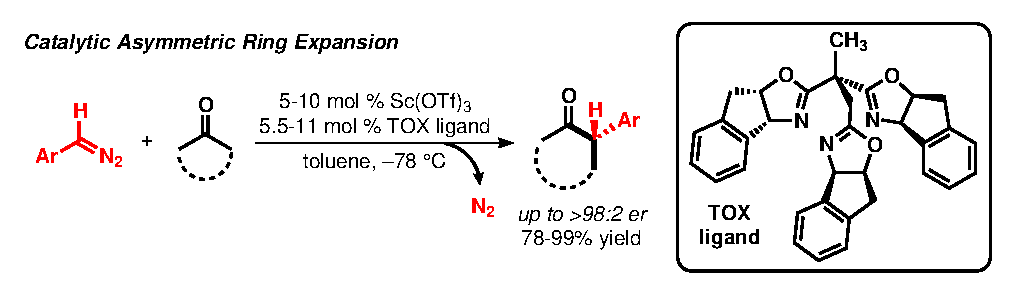
\includegraphics[scale=0.8]{chp_asymmetric_abstract}
\end{center}

\pagebreak
\thispagestyle{empty}
\noindent \ding{110} \textbf{Chapter 3.} Single-carbon ring expansion is a powerful synthetic
disconnection, allowing chemists to construct or purchase the lower homologue of a ring system before expanding to
the target ring size. Starting from a smaller ring size can often allow access to a broader array of
transformations that proceed with greater stereoselection.  In our approach to a class of natural
products bearing a \textit{cis}-decalin core, we successfully implemented a catalytic regioselective
single-carbon ring expansion reaction in the context of an advanced synthetic intermediate. This
chapter describes the experimental details behind the first catalytic single carbon cyclopentanone
homologations and how we extended the method to more complex substrates.

\begin{center}
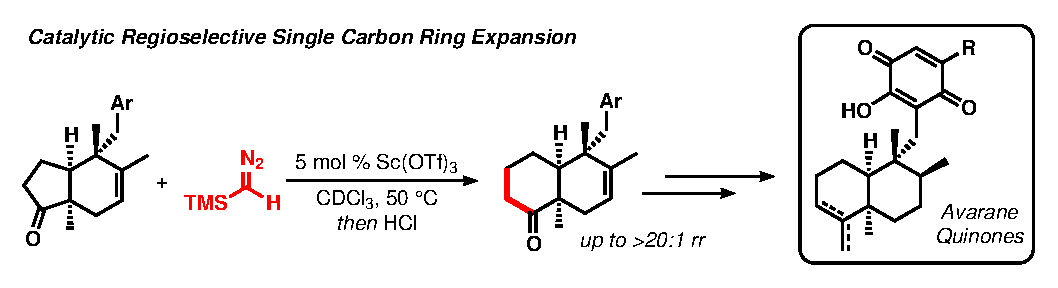
\includegraphics[scale=0.8]{chp_singlecarbon_abstract}
 \end{center}
 
 \singlespacing
 %%%%%%%%%%%%%%%%%%%%%%%%%%%%%%%%%%%%%%
 \pagebreak
\thispagestyle{empty} 
 \begin{center}
 \textsc{{\Large Catalysis of Etherification Reactions \\with sp$^3$
Electrophiles}}\\
\vspace{5mm}
\textbf{Victor L. Rendina} \\
\vspace{5mm}
\textbf{Thesis Advisors: Marc L. Snapper, Amir H. Hoveyda} \\ 
\vspace{5mm} 
\textbf{Abstract}
 \end{center}
 
 \doublespacing
 \noindent \ding{110} \textbf{Chapter 4.} Catalytic activation of \textit{sp$^2$} hybridized
 electrophiles by nucleophilic catalysts has been studied extensively and proceeds through a
 well-defined mechanistic pathway. In constrast, activation of \textit{sp$^3$} hybridized
 electrophiles in a similar fashion with small-molecule organocatalysts remains an elusive endeavor
 for chemists. This chapter describes preliminary studies towards this lofty goal and how we discovered a new class of imidazole-based catalysts. Thorough mechanistic studies with the newly discovered catalysts
 ultimately proved that the reactions proceeded through a pathway that does not involve electrophile
 activation. However, inexpensive and commercially available imidazolium salts were found to
 catalyze Williamson etherification reactions under mild conditions through a mechanism that involves an
 unusual imidazolium alkoxide ion-pair.
 
 \begin{center}
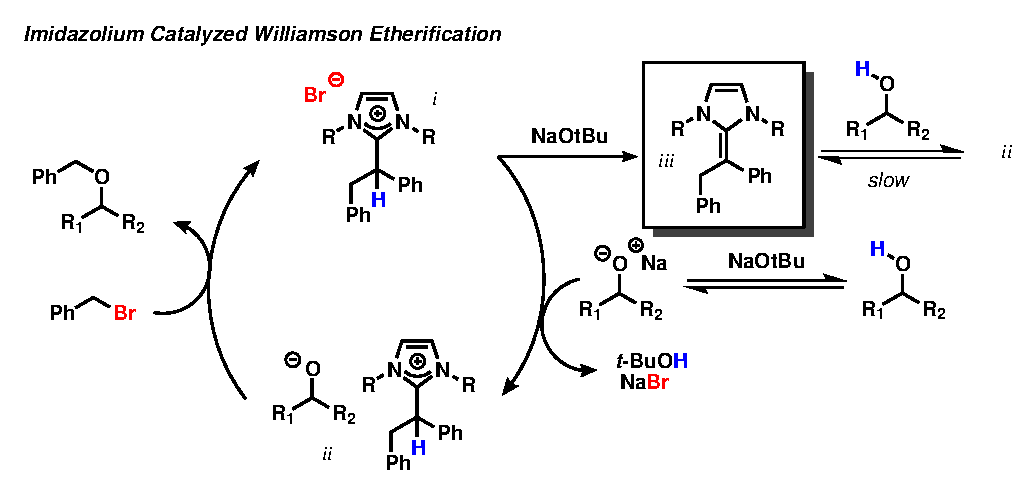
\includegraphics[scale=0.8]{chp_alkylation_abstract}
 \end{center}

 
 \singlespacing
\pagenumbering{roman}
\setcounter{page}{1}
% Print table of contents with consistent header
%\noindent {\Large \sffamily Contents}
\noindent \textsc{\Large Contents} \\
\hrule
\toccontents				%%% this is throwing a weird error
\noindent \textsc{\Large Acknowledgements} \\
\hrule
\vspace{5mm}
\doublespacing

I would like to first acknowledge Professor T. V. RajanBabu of The Ohio State University, for my
development as an organic chemist undoubtedly began in his laboratories as a young undergraduate
student. Professor RajanBabu, through his lectures and our discussions, instilled within me a great
sense of scientific virtue and rigor that I will carry with me for the rest of my life. It was
through his suggestion that I ended up applying for graduate school at Boston College.


At Boston College I have been fortunate to have worked with a number of distinguished faculty
members. Professor Jason Kingsbury has been, and continues to be a strong source of support as I
move forward with my career. As an advisor, Jason gave me a tremendous amount of intellectual
freedom and provided the environment and encouragement for my ideas to grow. He has an incredible
sense of compassion for his students and has always wanted the best for us. Professor Kian Tan,
through his own actions, taught me the importance of determination and hard work. Professor Lawrence
Scott has always been available to assist me with chemistry or publications to no benefit of his
own, and for that I am grateful. Professor Marc Snapper has a brilliant and unique perspective on
chemistry and learning from his approach has been an important part of my development as a
scientist. Professor Amir Hoveyda has a contagious sense of enthusiasm for chemistry and I feel
fortunate to have worked with him.


I would also like to thank all of the graduate and undergraduate students who have made my time at
Boston College more enjoyable. I have been very fortunate to have met several people in particular
through this process who have enriched my life in many ways. Hilan Kaplan is an exceptionally
skilled and passionate scientist who I have learned a great deal from through our discussions and
from working together. Hilan has been an incredible friend and we had a lot of fun together in the
Kingsbury lab. I was also lucky to have the opportunity to work with Bowman Potter, who has become a
great friend as well. My time spent in the Snapper lab was more enjoyable because of Bowman, and his
dedication was inspirational towards the end of my graduate career. In the Kingsbury and Snapper
labs we never had a lot of resources, but with both Hilan and Bowman, we were able to work as a
close team and accomplish far more than what we ever could have done individually.


Finally, I would like to acknowledge a very special relationship with Samantha Goetz that has had a
profound impact on my life over the past few years. Samantha is a highly competent and conscientious
chemist who is always thinking and asking the right questions. Her curiosity has forced me
reevaluate many aspects of chemistry where I had since become complacent. Outside of the lab,
Samantha is one of the most compassionate people I have ever encountered. I am forever indebted to
her love and support, which has helped make this work possible.




\noindent\textsc{{\Large List of Abbreviations}}\\
\hrule
\doublespacing
\vspace{10pt}
{%\small %\singlespacing
\begin{supertabular}{p{1.5in}l}
[$\alpha$] & specific rotation \\
\AA&angstrom \\
$\phi$&diameter\\
Ac&acetyl\\
acac&acetylacetonyl\\
AIBN&2,2'-azobis(2-methylpropionitrile)\\
Ar&aryl (substituted aromatic ring)\\
B(Ar$^\mathrm{F}$)$_4$&tetrakis[(3,5-trifluoromethyl)phenyl]borate\\
BINAP&2,2'-bis(diphenylphosphino)-1,1'-binaphthyl\\
BINOL&1,1'-bi-2-naphthol\\
bm &broad medium (IR)\\
Bn&benzyl\\
Boc&\textit{tert}-butoxycarbonyl\\
BOX&bis(oxazoline)\\
brsm & based on recovered starting material \\
bs&broad strong (IR)\\
Bu&butyl\\
bw&broad weak (IR)\\
calcd & calculated \\
CAN&cerium(IV) ammonium nitrate\\
conv & conversion \\
d&day(s); doublet (NMR)\\
dba&dibenzylideneacetone\\
DCA&dichloroethane\\
DCC&dicyclohexylcarbodiimide\\
dd&doublet of doublets (NMR)\\
ddd&doublet of doublet of doublets (NMR)\\
dddd&doublet of doublet of doublet of doublets (NMR)\\
DIPEA&\textit{N},\textit{N}-diisopropylethylamine\\
DMAP&4-dimethylaminopyridine\\
DME&1,2-dimethoxyethane\\
DMF&\textit{N},\textit{N}-dimethylformamide\\
DMP&Dess-Martin periodinane\\
DMS&dimethylsulfide\\
DMSO&dimethylsulfoxide\\
DPEN&1,2-diphenyl-1,2-diaminoethane\\
dr&diastereomeric ratio\\
EDC&1-ethyl-3-(3-dimethylaminopropyl)carbodiimide\\
equiv&equivalent(s)\\
er&enantiomeric ratio\\
ESI$+$&electrospray ionization (positive ion mode) \\
Et&ethyl\\
g&grams(s)\\
GC&gas chromatography\\
h&hour(s)\\
hfac&hexafluoroacetylacetone \\
HMPA&hexamethylphosphoramide\\
HRMS&high resolution mass spectrometry\\
\textit{i}-Pr&isopropyl\\
IMes&1,3-bis(2,4,6-trimethylphenyl)imidazolium\\
IR&infrared spectroscopy\\
\textit{J}&coupling constant in Hz (NMR)\\
L & liter(s) \\
LAH&lithium aluminum hydride\\
LDA&lithium diisopropylamide\\
LUMO&lowest unoccupied molecular orbital\\
M & molarity (mol / L); molecular formula (HRMS) \\ 
\textit{m}&\textit{meta}\\
m&milli; multiplet (NMR); medium (IR)\\
\textit{m}-CPBA&\textit{meta}-chloroperbenzoic acid\\
MAD&methylaluminum bis(2,6-di-\textit{tert}-butyl-4-methylphenoxide)\\
Me&methyl\\
MHz & megahertz \\
min&minute(s)\\
mol&mole(s)\\
\textit{n}&normal (unbranched alkyl chain)\\
NBS&\textit{N}-bromosuccinimide\\
NCS&\textit{N}-chlorosuccinimide\\
NMR&nuclear magnetic resonanace\\
\textit{o}&\textit{ortho} \\
ORTEP&Oak Ridge thermal ellipsoid plot\\
\textit{p}&\textit{para} \\
p&pentet (NMR)\\
PCC&pyridinium chlorochromate\\
PDMS&phenyldimethylsilyl\\
PDMSD&phenyldimethylsilyldiazomethane\\
Pent&pentyl\\
Ph&phenyl\\
PHOX&phosphinooxazoline\\
PPTS&pyridinium \textit{para}-toluenesulfonate\\
PPY&4-pyrrolidinopyridine\\
Pr&propyl\\
PyBOX&2,6-bis(oxazolinyl)pyridine\\
q&quartet (NMR)\\
qd & quartet of doublets (NMR) \\
Red-Al&sodium bis(2-methoxyethoxy)aluminum hydride\\
rr & regioisomeric ratio \\
s&singlet (NMR); strong (IR)\\
SAMP&(\textit{S})-1-amino-2-(methoxylmethyl)pyrrolidine\\
sept&septet (NMR) \\
SFC&supercritical fluid chromatography\\
\textit{t}&tertiary alkyl chain \\
t & triplet (NMR)\\
TBAF&tetra-\textit{n}-butylammonium fluoride\\
TBAI&tetra-\textit{n}-butylammonium iodide\\
TBDPS&\textit{tert}-butyldiphenylsilyl\\
TBS&\textit{tert}-butyldimethylsilyl\\
td & triplet of doublets (NMR) \\
temp & temperature \\
Tf&trifluoromethanesulfonyl\\
THF&tetrahydrofuran\\
TLC&thin layer chromatography\\
TMG&1,1,3,3-tetramethylguanidine\\
TMHD&2,2,6,6-tetramethylheptane-3,5-dionate\\
TMS&trimethylsilyl\\
TMSD&trimethylsilyldiazomethane\\
TOX&tris(oxazoline)\\
Ts&\textit{para}-toluenesulfonyl\\
tt&triplet of triplets (NMR)\\
v/v&volume / volume\\
w&weak (IR)\\
w/w&weight / weight\\
\end{supertabular}
}
%%% Setup the headers
\pagebreak
\pagestyle{fancy}
\renewcommand{\headrulewidth}{0pt}
\renewcommand{\sectionmark}[1]{\markright{#1}}
\lhead{\footnotesize \textsc{\thesection \hspace{2mm} \rightmark}}
%\rhead{\textit{\footnotesize \sffamily \textbf{Chapter \thechapter}\\ Page
%\thepage}}
\rhead{\footnotesize  \textsc{Chapter \thechapter} \hspace{2mm} {\huge$|$} \hspace{2mm}
\textsc{\textbf{\thepage}}}
\cfoot{}
\pagenumbering{arabic}
%%% Chapter includes
%%% Reset counters for the footnotes and compound numbering
%\setcounter{compound}{0}
\stepcounter{cmpreset}
\captionsetup[figure]{list=no} % hide figures from list in experimental section

\chapter{History of Ring Expansion Reactions with Non-stabilized Diazoalkanes}
\label{chp:diazobkg}
 %\thispagestyle{empty}
 \pagebreak
 
\section{Introduction}
\doublespacing The synthesis of the first
diazoalkanes dates back over 100 years and began with the preparation of ethyl diazoacetate by Curtius,\footnote{{\frenchspacing Curtius, T. Ueber die
Einwirkung von salpetriger S\"{a}ure auf salzsauren Glycocoll\"{a}ther. \textit{Ber. Dtsch. Chem.
Ges.} \textbf{1883}, \textit{16}, 2230-2231.}} followed later with the synthesis of diazomethane by
Pechmann.\footnote{{\frenchspacing Pechmann, H. V. Ueber Diazomethan. \textit{Ber. Dtsch. Chem.
Ges.} \textbf{1891}, \textit{27}, 1888-1891.}} Diazo compounds have since become an exceptionally
versatile and important building block in synthetic organic chemistry. The ambiphilic nature of the
diazo functional group has provided access to a wide array of transformations (e.g.
\ce{C-H}, \ce{N-H}, and \ce{O-H} insertion, ylide formation, cyclopropanation, 1,3-dipolar
cycloadditions) and their use has been extensively reviewed.\footnote{For lead references
refer to: (a) Regitz, M.; Maas, G. \textit{Diazo Compounds$-$Properties and Synthesis}; Academic
Press: Orlando, 1986. (b) Doyle, M. P.; McKervey, M. A.; Ye, T. \textit{Modern Catalytic Methods for
Organic Synthesis with Diazo Compounds}; Wiley: New York, 1998.} Although it is generally accepted
that diazo compounds are toxic and unstable,\footnote{For a very thorough discussion of diazomethane
safety see: {\frenchspacing Proctor, L. D.; Warr, A. J. Development of a Continuous Process for the
Industrial Generation of Diazomethane. \textit{Org. Process Res. Dev.} \textbf{2002}, \textit{6},
884-892.}} their lability is largely correlated with the electronic properties of the flanking
functional groups. Diazoalkanes with neighboring electron-withdrawing groups (carbonyl, phosphoryl,
sulfonyl) are typically more stable and several such diazoalkanes have become commercially
available (\reffigure{commercial}). With the exception of
TMSD (\ref{cmp:aaa}), all of the commercially available diazo compounds are stabilized by an
electron-withdrawing carbonyl moiety. The relatively stable $\alpha$-diazocarbonyl compounds, although less reactive, are still utilized in many of the same
transformations as their more reactive noncarbonyl-stabilized counterparts.\footnote{{\frenchspacing
Ye, T.; McKervey, M. A. Organic Synthesis with $\alpha$-Diazo Carbonyl Compounds. \textit{Chem. Rev.}
\textbf{1994},
\textit{94}, 1091-1160.}}

\begin{figure}[b]
  \centering
  \includegraphics[scale=0.8]{chp_diazobkg/images/commercialdiazos}
  \begin{textblock}{1}(17.2,-0.25) \cmp{aaa} \end{textblock}
  \caption{Commercially available diazoalkanes.}
  \label{fig:commercial}
\end{figure}

 \begin{figure}[t]
  \centering
  \includegraphics[scale=0.8]{chp_diazobkg/images/nucleophilicity}
  \begin{textblock}{1}(3,-1.2) \cmp{aaaa} \end{textblock}
  \caption{Nucleophilicity parameters of several diazoalkanes.}
  \label{fig:nucleophilicity}
\end{figure}
The nucleophilicity, and thus reactivity,
of the diazo functional group is highly dependent upon the adjacent functional groups and has been
found to span a fairly broad range of values. 
Careful kinetics experiments carried out by Mayr and coworkers established a series of relative
diazoalkane nucleophilicity parameters (\reffigure{nucleophilicity}).\footnote{\frenchspacing{Bug,
T.; Hartnagel, M.; Schlierf, C.; Mayr, H. How Nucleophilic Are Diazo Compounds? \textit{Chem. Eur.
J.} \textbf{2003}, \textit{9}, 4068-4076.}} At the most reactive end of the spectrum, the
nucleophilicity of diazomethane was found to be comparable to the enamine functional group. While at
the other end of the reactivity spectrum, diethyl 2-diazomalonate (\ref{cmp:aaaa})
was found to have a nucleophilicity similar to styrene. Using this scale as a
general guideline, diazoalkanes can be classfied into two primary categories. Those referred to as
stabilized diazoalkanes are diazo compounds  adjacent to a carbonyl, phosphoryl, or sulfonyl moeity
(\textit{N}$<$5). The content of this thesis will focus primarily on the utility of the more
reactive non-stabilized diazoalkanes, those typically bearing adjacent alkyl or aryl substituents (\textit{N}$>$5). The relative instability and toxicity
of non-stabilized diazoalkanes has limited their synthetic value, however, the recent
development of mild methods for their preparation has facilitated a renewed interest
in methodologies based on these unique molecules.\footnote{For a recent review see:
\frenchspacing{Maas, G.
New Syntheses of Diazo Compounds.
\textit{Angew. Chem. Int. Ed.} \textbf{2009},
\textit{48}, 8186-8195.}} 

This chapter will present a brief historical
account of the most significant developments in non-stabilized diazoalkane chemistry, with a
specific focus on ring expansion methodology. The discussion opens with some of the first reactions of diazoalkanes, discovered more than a century ago, and ultimately culminates in the discovery of
mild and catalytic methods for ring expansion first disclosed by our research group nearly 125 years
later.


% \pagebreak
% % %%%%%%%%%%%%%%%%%%%%%%%%%%%%%%%%%%%%%%%%%%%%%%%%%%%%%%%%%%%%%%%%%%%%%%%%%%%%%%%%%%%%%%%%%%%%%%%%%
% % %%%%%%%%%%%%%%%%%%%%%%%%%%%%%%%%%%%%%%%%%%%%%%%%%%%%%%%%%%%%%%%%%%%%%%%%%%%%%%%%%%%%%%%%%%%%%%%%%
% % %%%%%%%%%%%%%%%%%%%%%%%%%%%%%%%%%%%%%%%%%%%%%%%%%%%%%%%%%%%%%%%%%%%%%%%%%%%%%%%%%%%%%%%%%%%%%%%%%
% \section{Preparative Methods for Non-Stabilized Diazoalkanes}
% The handling of noncarbonyl-stabilized diazoalkanes as neat compounds is often
% impractical and potentially hazardous. Neat diazomethane is a dangerous and
% highly toxic gas that has been the culprit in a number of violent and
% unpredictable explosions.\footnote{} Although higher molecular weight derivates
% are often oils or solids at room temperature, bimolecular decomposition pathways
% are common and accelerated if the compounds are stored in the absence of
% solvent.\footnote{} For this reason, diazoalkanes have been generated for use in
% situ by elimination of \textit{N}-nitroso compounds,\footnote{} Bamford--Stevens
% decomposition,\footnote{} iodine(III)-mediated oxidation of
% \textit{N}-silylhydrazones,\footnote{} or the decomposition of
% \textit{N}-aziridinylimines.\footnote{} Alternatively, mild methods based on
% free hydrazone oxidation\footnote{} or diazo transfer\footnote{} facilitate
% access to pure solutions that can be stored at low temperatures. Figure xxx
% highlights some of the key methods for diazoalkane synthesis: (A) (B) (C) (D)
% (E) (F). A discussion of several of these preparative methods is provided in the
% sections that follow.
% %\subsection{Elimination of \textit{N}-Nitroso Compounds}
% %\subsection{Bamford-Stevens Decomposition}
% %\subsection{Direct Hydrazone Oxidation}



\pagebreak
%%%%%%%%%%%%%%%%%%%%%%%%%%%%%%%%%%%%%%%%%%%%%%%%%%%%%%%%%%%%%%%%%%%%%%%%%%%%%%%%%%%%%%%%%%%%%%%%%%
%%%%%%%%%%%%%%%%%%%%%%%%%%%%%%%%%%%%%%%%%%%%%%%%%%%%%%%%%%%%%%%%%%%%%%%%%%%%%%%%%%%%%%%%%%%%%%%%%%
%%%%%%%%%%%%%%%%%%%%%%%%%%%%%%%%%%%%%%%%%%%%%%%%%%%%%%%%%%%%%%%%%%%%%%%%%%%%%%%%%%%%%%%%%%%%%%%%%%

\section{History of Diazoalkane Ring Expansion Reactions}
The reaction of diazoalkanes with carbonyl-containing compounds dates back to
observations made by Buchner and Curtius as early as
1885.\footnote{\frenchspacing{Buchner, E.; Curtius, T. Synthese von
Ketons\"{a}ure\"{a}thern aus Aldehyden und Diazoessig\"{a}ther. \textit{Ber.
Dtsch. Chem. Ges.} \textbf{1885}, \textit{18}, 2377-2379.}} Although others
examined this novel reactivity pattern,\footnote{(a) \frenchspacing{Pechmann, H.
V.; Frobenius, L. Nachtr\"{a}gliches \"{U}ber Aromatische Diazoverbindungen.
\textit{Ber. Dtsch. Chem. Ges.} \textbf{1895}, \textit{28}, 170-176}. (b)
\frenchspacing{Meyer, H. \"{U}ber die Einwirkung von Diazomethan auf
Aldehyds\"{a}uren und Aldehyde. \textit{Monatsh. Chem.} \textbf{1905},
\textit{26}, 1295-1301.}} Schlotterbeck is largely credited with discovering the
reaction of aldehydes with diazoalkanes in 1907.\footnote{(a) \frenchspacing{Schlotterbeck, F.
Umwandlung von Aldehyden in Ketone durch Diazomethan. \textit{Ber. Dtsch. Chem. Ges.}
\textbf{1907}, \textit{40}, 479-483}. (b) \frenchspacing{ Schlotterbeck, F.
Umwandlung von Aldehyden in Ketone durch Diazomethan. II.
\textit{Ber. Dtsch. Chem. Ges.} \textbf{1909}, \textit{42}, 2559-2564.}}
Schlotterbeck was able to confirm through careful experimentation that various
aliphatic aldehydes afforded the corresponding methyl ketones when treated with
diazomethane. The reaction of aldehydes with diazomethane to form methyl ketones
later became known as the Buchner-Curtius-Schlotterbeck
reaction (\refscheme{bcs}).\footnote{\frenchspacing{Eistert, B.
In \textit{Newer Methods of Preparative Organic Chemistry,} English ed.; New York, 1948; p
521.}} Application of this method to ketone substrates and eventually cyclic
ketones did not come until several decades later and required a critical new
discovery. 

\begin{Scheme}[ht]
  \centering
  \includegraphics[scale=0.8]{chp_diazobkg/images/bcs}
  \caption{The Buchner-Curtius-Schlotterbeck Reaction}
  \label{sch:bcs}
\end{Scheme}

\subsection{Protic Solvent Promoted Reactions}
In 1928 Meerwein recorded one of the first reactions of
diazomethane with a ketone, promoted by the presence of a protic solvent.\footnote{(a)
\frenchspacing{Meerwein, H.; Burneleit, W. \"{U}ber die Einwirkung von Diazomethan auf Ketone in Gegenwart von
Katalysatoren. \textit{Ber. Dtsch. Chem. Ges.} \textbf{1928}, \textit{61},
1840-1847}. (b) \frenchspacing{Meerwein, H. Verfahren zur Umsetzung Organischer
Verbindungen mit Diazomethan. German Patent 579,309, June 26, 1933}.
\label{ref:meerwein}} When acetone was treated with diazomethane no reaction
occurred, however, in the presence of water or alcohols dimethylethylene oxide
and 2-butanone were readily produced (\refscheme{meerwein}). This important new
discovery could be rationalized by invoking a model based on general acid catalysis. Assuming the
reaction mechanism proceeds through an initial slow addition of diazomethane to the carbonyl, protic
solvents can facilitate this addition by hydrogen bonding to the incipient alkoxide, thereby
enhancing the electrophilicity of the carbonyl acceptor.
\begin{Scheme}[t]
  \centering
  \includegraphics[scale=0.8]{chp_diazobkg/images/meerwein}
  \caption{Discovery of protic solvent catalysis.}
  \label{sch:meerwein}
\end{Scheme}

Following Meerwein's crucial discovery of protic solvent catalysis,
Mosettig\footnote{\frenchspacing{Mosettig, E.; Burger, A. Ring Enlargement With Diazomethane in the Hydroaromatic Series. \textit{J. Am. Chem. Soc.} \textbf{1930}, \textit{52}, 3456-3463.} \label{ref:mosettig}} reported the first carbocyclic ring expansions.\footnote{Heller had observed the production of dihydroxyquinoline
from isatin several years prior to Mosettig's work. (a) \frenchspacing{Heller,
G. Neue \"{U}berg\"{a}nge aus der Indol- in die Chinolin-Reihe. \textit{Ber.
Dtsch. Chem. Ges.} \textbf{1919}, \textit{52}, 741-745}. (b)
\frenchspacing{Heller, G. Neue \"{U}berg\"{a}nge aus der Indol- in die
Chinolin-Reihe II. (Nach Versuchen von Rudolph Fuchs, Paul Jacobsohn, Martin
Raschig und Elsbeth Sch\"{u}tze). \textit{Ber. Dtsch. Chem. Ges.}
\textbf{1926}, \textit{59}, 704-710.}} Cyclohexanone, when combined with excess
diazomethane in ethereal solvents, was completely unreactive.\footnote{A later
report indicated that cyclohexanone would undergo ring expansion with
diazoethane in the absence of protic catalysis to produce 2-methylcycloheptanone
as the primary product. \frenchspacing{Giraitis, A. P.; Bullock, J. L.
Reactions of Cyclohexanone With Diazoethane. \textit{J. Am. Chem. Soc.}
\textbf{1937}, \textit{59}, 951-951.}} Upon the addition of methanol, nitrogen
gas evolved vigorously and the production of cycloheptanone, cyclooctanone, and an epoxide
isomeric with cycloheptanone were observed (\refscheme{mosettig}).
\begin{Scheme}[b]
  \centering
  \includegraphics[scale=0.8]{chp_diazobkg/images/mosettig}
  \caption{First example of carbocyclic ring expansions with diazomethane.}
  \label{sch:mosettig}
\end{Scheme}
When the same reaction was carried out starting with cyclopentanone (n = 0),
cycloheptanone and cyclooctanone were again the primary products. Residual cyclopentanone and cyclohexanone were not detected, thus indicating
complete consumption of the starting material and subsequent homologation of the
intermediate cyclohexanone. Addition of diazomethane to cyclopentanone increases torsional strain by
introducing an additional \textit{sp$^3$} hybridized center within the confined ring system. 
Cyclohexanone is generally regarded as more reactive due to the staggered nature of all bonds upon
addition of diazomethane.\footnote{\frenchspacing{Gutsche, C. D.
The Reaction of Diazomethane and Its Derivatives with Aldehydes and Ketones.
\textit{Org. React.} \textbf{1954}, \textit{8}, 364-403.} \label{ref:gutschereview}} This early
example serves to illustrate three fundamental challenges with the diazoalkane carbonyl homologation reaction: (1)
controlling the ring size is difficult when the products are more reactive than the starting
materials -- the products generated possess an identical functional group ready for further
reaction (2) formation of oxirane byproducts is often unavoidable (3) an excess of diazomethane is typically
used because the reagent decomposes in the reaction timeframe.

 \begin{Scheme}[b]
  \centering
  \includegraphics[scale=0.8]{chp_diazobkg/images/adamsonkenner}
\begin{textblock}{1}(3.2,-1.4) \cmp{aab} \end{textblock}
\begin{textblock}{1}(6.1,-1.4) \cmp{aac} \end{textblock}
\begin{textblock}{1}(11.0,-1.4) \cmp{aad} \end{textblock} 
\begin{textblock}{1}(13.8,-1.4) \cmp{aae} \end{textblock}  
\begin{textblock}{1}(16.7,-1.4) \cmp{aaf} \end{textblock}
  \caption{First ring expansion of a 2-substituted cycloalkanone.}
  \label{sch:adamsonkenner}
\end{Scheme}
Mosettig's first reactions, and subsequent ring expansions,\footnote{Several
medium ring cycloalkanones were prepared on kilogram scale following Meerwein's
procedures (reference \ref{ref:meerwein}b). \frenchspacing{Kohler, E. P.;
Tishler, M.; Potter, H.; Thompson, H. T. The Preparation of Cyclic Ketones by Ring Enlargement. \textit{J. Am. Chem.
Soc.} \textbf{1939}, \textit{61}, 1057-1061.}} were limited to symmetrical
cycloalkanones. It was not until nearly a decade later that Adamson and
Kenner reported the homologation of 2-methylcyclohexanone with
diazomethane (\refscheme{adamsonkenner}).\footnote{\frenchspacing{Adamson, D.
W.; Kenner, J. Reactions of Aliphatic Diazo-compounds with Carbonyl Derivatives.
\textit{J. Chem. Soc.} \textbf{1939}, 181-189.} \label{ref:adamsonkenner}} Generation of
diazomethane
\textit{in situ} from \textit{N}-nitrosomethylurethane\crossref{ref:meerwein}
(\ref{cmp:aac}) in the presence of 2-methylcyclohexanone (\ref{cmp:aab}) produced both possible
regioisomers of the ring expanded products (\ce{->}\ref{cmp:aad} + \ref{cmp:aae}) in a combined 37\%
yield along with an equivalent yield of epoxide \ref{cmp:aaf}. The 2-- and 3-substituted
cycloheptanones were separated and positively identified by selective formation
of a bisulfite adduct, however, the regioisomeric ratio was not clearly
reported.


\begin{Scheme}[b]
  \centering
  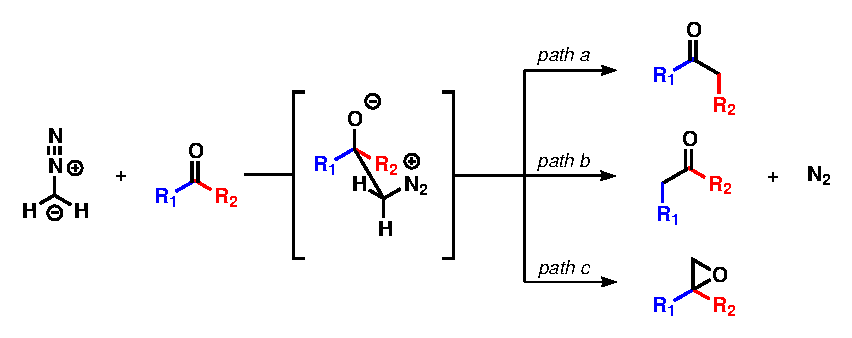
\includegraphics[scale=0.8]{chp_diazobkg/images/mechanism}
  \begin{textblock}{1}(5.5,-1.0) \cmp{aag} \end{textblock}
  \begin{textblock}{1}(8.7,-1.0) \cmp{aah} \end{textblock}
  \caption{Mechanism for the diazoalkane carbonyl homologation
  reaction.}
  \label{sch:mechanism}
\end{Scheme}
In 1949, Gutsche began to carefully examine the regiochemical outcome when
various 2-aryl substituted cyclohexanones were homologated with
diazomethane.\footnote{(a)
\frenchspacing{Gutsche, C. D. Ring Enlargements I. The Ring Enlargement of 2-Chlorocyclohexanone and 2-Phenylcyclohexanone. \textit{J. Am. Chem. Soc.}
\textbf{1949}, \textit{71}, 3513-3517}. (b) \frenchspacing{Gutsche, C. D.;
Strohmayer, H. F.; Chang, J. M. Ring Enlargements VI. The Diazomethane-Carbonyl
Reaction: Product Ratios from the Reactions of Diazomethane with Various
Substituted 2-Phenylcyclohexanons. \textit{J. Org. Chem.} \textbf{1958},
\textit{23}, 1-5.} \label{ref:gutschetwo}} The accepted mechanism at the time,
based primarily on qualitative data,\crossref{ref:gutschereview} is depicted below in
\refscheme{mechanism}. Initial rate limiting addition of the diazoalkane
nucleophile, followed by concerted collapse of betaine intermediate
\ref{cmp:aah},\footnote{Intermediate \ref{cmp:aah} resembles the same
intermdiate believed to exist in the Tiffeneau-Demjanov reaction. For a review see: \frenchspacing{Smith, P. A. S.; Baer, D. R. The Demjanov and Tiffeneau-Demjanov Ring Expansions. \textit{Org. React.} \textbf{1960}, \textit{11}, 157-180.}\\
\includegraphics[scale=0.7]{chp_diazobkg/images/tiffeneaudemjanov}} could lead
to three possible products. Gutsche hypothesized that by modifying
the electronics at R$_1$ and R$_2$ in ketone \ref{cmp:aag}, the more electron
rich group would migrate preferentially. The results of his findings, along
with the corresponding Hammett $\rho$ values\footnote{\frenchspacing{Hammett, L.
P. The Effect of Structure upon the Reactions of Organic Compounds. Benzene
Derivatives. \textit{J. Am. Chem. Soc.} \textbf{1937}, \textit{59}, 96-103.}}
are summarized in \reftable{gutschereg}. 
\begin{table}[ht] \centering
\vspace{10pt}
\includegraphics[scale=0.8]{chp_diazobkg/images/gutsche}
\begin{textblock}{1}(6.35,-1.8) \textsf{\scriptsize{\ref{cmp:aac}}}
\end{textblock}
\begin{textblock}{1}(4.7,0.2) \cmp{aai} \end{textblock}
\begin{textblock}{1}(10.0,0.2) \cmp{aaj} \end{textblock}
\begin{textblock}{1}(13.1,0.2) \cmp{aak} \end{textblock}
\begin{textblock}{1}(15.9,0.2) \cmp{aal} \end{textblock}
\vspace{15pt}
{\footnotesize
\begin{tabular}{ccccccc}
\toprule
entry & G & $\rho$ & \ref{cmp:aaj} (\%) & \ref{cmp:aak} (\%) & \ref{cmp:aal}
(\%) & rr (\ref{cmp:aaj}:\ref{cmp:aak})
\\
\midrule
\rowcolor{gray!15}1&H&0& 59 & 14 & 21 & 4.2:1 \\
2&\textit{p}-\ce{CH3}&$-$0.170& 55 & 20 & 21 & 2.8:1 \\
3&\textit{p}-\ce{OCH3}&$-$0.268& 57 & 21 & 14 & 2.7:1 \\
4&2,3,4-\ce{OCH3}&-& 40  & 28 & 18 & 1.4:1  \\
5&\textit{p}-Cl&$+$0.227& 45 & 20 & 26 & 2.2:1 \\
\bottomrule
\end{tabular}
}
\caption{Early regiochemical investigations by Gutsche and coworkers.}
\label{tbl:gutschereg}
\end{table}

It was anticipated based on this electronic argument that entry 5 (G = \textit{p}-Cl) would show
the highest levels of regioselectivity, with preferential migration of the less substituted carbon.
Entry 4 (G = 2,3,4-OCH$_3$) was expected to show the lowest levels of regiocontrol, or potentially
an inversion of selectivity, favoring migration of the aryl substituted carbon.
Unfortunately, the data were inconclusive and attempts were made to rationalize the results. The
highest level of regioselectivity was observed for entry 1 (G = H), not entry 5 (G =
\textit{p}-Cl). The lowest level of selectivity was observed in entry 4 as
expected, but regardless, there appeared to be little difference between the values in each entry. Gutsche
proposed that three factors were important to determine which bond will migrate from betaine
intermediate \ref{cmp:aah}: (1) the relative electron-releasing ability of R$_1$, R$_2$, and oxygen,
(2) the strain involved in the transition state, (3) and the steric and electronic environment
around the diazonium. Gutsche concluded that the reactions were largely insensitive to electronic
perturbations of the aromatic ring and the observed selectivities must be the result of counterbalancing each of these factors. In general though, there was a strong intrinsic regiochemical preference for migration of the less substituted group, regardless of the electronic perturbations.\footnote{The Baeyer-Villiger oxidation typically displays
the oppposite regiochemical preference for differentially substituted ketones. {\frenchspacing Krow,
G.
R.
The Baeyer-Villiger Oxidation of Ketones and Aldehydes. In \textit{Organic Reactions;} Paquette, L. A., Ed.; Wiley: New York,
1993; Vol. 43; p 251.}}


Gutsche also examined a variety of aryl-substituted diazo compounds and reported
some of the first examples of protic solvent catalyzed reactions with substituted diazoalkanes
(\refscheme{gutorgsyn}).\footnote{(a) \frenchspacing{Gutsche, C. D.; Johnson, H. E. Ring Enlargements. III. Ring Enlargement of Cyclohexanone with Ethyl
\textit{N}-Nitroso-\textit{N}-Benzylcarbamates Carrying Methyl and Methoxyl
Substituents on the Phenyl Nucleus. \textit{J. Am. Chem. Soc.} \textbf{1955}, \textit{77}, 109-112.} (b)
\frenchspacing{Gutsche, C. D.; Johnson, H. E. 2-Phenylcycloheptanone.
\textit{Org. Synth.} \textbf{1955}, \textit{35}, 91.} (c) \frenchspacing{
Gutsche, C. D.; Jason, E. F. Ring Enlargements. V. The Preparation of
2-Arylcycloheptanones and 2-Aryl-2-cycloheptenones. \textit{J. Am. Chem. Soc.}
\textbf{1956},
\textit{78}, 1184-1187.} \label{ref:gutsub}} Although a number of examples were
reported, the most striking example was the large scale preparation of
2-phenylcycloheptanone (\ref{cmp:aan}) by the \textit{in situ} generation of
phenyldiazomethane from ethyl
\textit{N}-nitroso-\textit{N}-benzylcarbamate
(\ref{cmp:aam}).\crossref{ref:gutsub}\textsuperscript{b} The yield was
moderate, however, over 150 grams of product were obtained in a single run. In addition
to the desired product, methyl benzyl ether (\ref{cmp:aao}) was also obtained in
a 25\% yield, highlighting one of the serious complications with protic solvent
based catalysis.
\begin{Scheme}[h]
  \centering
  \includegraphics[scale=0.8]{chp_diazobkg/images/gutorgsyn}
  \begin{textblock}{1}(6.3,-1.5) \cmp{aam} \end{textblock}
  \begin{textblock}{1}(12.6,-1.5) \cmp{aan} \end{textblock}
  \begin{textblock}{1}(16,-1.5) \cmp{aao} \end{textblock}
  \caption{Large scale preparation of 2-phenylcycloheptanone.}
  \label{sch:gutorgsyn}
\end{Scheme}



Expanding upon Gutsche's studies directed at elucidating regiochemical
preferences, Greene later found that $\alpha$,$\alpha$-dichlorocyclobutanones
afforded products resulting from preferential migration of the more electron rich
\ce{C-C} bond (\refscheme{greene},
\ref{cmp:aap}\ce{->}\ref{cmp:aaq}).\footnote{\frenchspacing{Greene, A. E.;
Depres, J. P. A Versatile Three-Carbon Annelation. Synthesis of Cyclopentanones and Cyclopentanone Derivatives from Olefins. \textit{J. Am.
Chem. Soc.} \textbf{1979}, \textit{101}, 4003-4005.} \label{ref:greene}} Common
epoxide byproducts were not observed, presumably due to the ring strain involved in
constructing a [2.3] spirocyclic system.\footnote{Jaz made a similar observation
with the ring expansion of cyclobutanone. \frenchspacing{Jaz, J.;
Davreux, J. P. Reactions Des Diazoalcanes Sur Les Cyclanones I. Action Du
Diazomethane Sur La Cyclobutanone. \textit{Bull. Chim. Soc. Belg.}
\textbf{1965}, \textit{74}, 370-379.}} Greene also noted a significant rate
acceleration for the electron deficient cyclobutanones, consistent with a rate
limiting intial addition step. The rate enhancement could be attributed to carbonyl-$\pi$
electron donation into the adjacent \ce{C-Cl} $\sigma$* orbital and increased
polarization of the \ce{C-O} bond through inductive effects. In this system, the
electronics of the cyclobutanone had a significant impact on the observed
regioselectivity. The des-chloro cyclobutanone \ref{cmp:aas} resulted in a 55:45
mixture of regioisomers, slightly favoring the production of
\ref{cmp:aaq}.\footnote{Unexpectedly, the Tiffeneau-Demjanov rearrangement of
\ref{cmp:aas} produced primarily the $\alpha$-ketone product in an 85:15 ratio
(determined by IR spectroscopy). \frenchspacing{Roberts, J. D.; Gorham, W. F.
Syntheses of Some Bicyclo [3.3.0]octane Derivatives. \textit{J. Am. Chem. Soc.}
\textbf{1952}, \textit{74},
2278-2282.}\\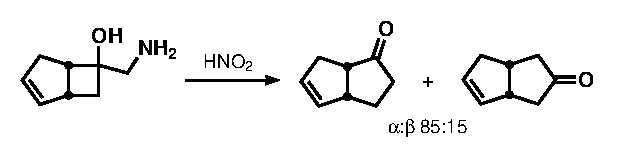
\includegraphics[scale=0.7]{chp_diazobkg/images/roberts}} With a
single chlorine (\ref{cmp:aar}), a 90:10 ratio was observed. The highest
selectivity was observed with \ref{cmp:aap}, affording predominantly the
$\beta$-ketone \ref{cmp:aaq} in a 95:5 regioisomeric ratio after reductive dehalogenation.
\begin{Scheme}[h]
  \centering
  \includegraphics[scale=0.8]{chp_diazobkg/images/greene}
  \begin{textblock}{1}(9.3,-3.6) \cmp{aap} \end{textblock}
  \begin{textblock}{1}(15.3,-3.6) \cmp{aaq} \end{textblock}
  \begin{textblock}{1}(9.5,-1) \cmp{aar} \end{textblock}
  \begin{textblock}{1}(12.7,-1) \cmp{aas} \end{textblock}
  \begin{textblock}{1}(6,-1) \textsf{\scriptsize{\ref{cmp:aap}}} \end{textblock}
  \caption{High levels of regiocontrol with
  $\alpha$,$\alpha$-dichlorocyclobutanones.}
  \label{sch:greene}
\end{Scheme}


\subsection{Lewis-acid Promoted Reactions}
While usage of a protic solvent was the premier means of accelerating diazoalkane ring
expansions for more than half a century, serious deficiencies limited the preparative value of these
transformations. As discussed in the previous section, early reactions suffered from low reaction rates, O\ce{-}H insertion byproducts, multiple homologations, regiochemical issues, and low efficiencies with more sterically demanding or
more substituted diazoalkanes. Early mechanistic data suggested that the initial carbonyl addition
event to form the diazonium betaine intermediate was rate limiting (\ce{->}\ref{cmp:aah},
\refscheme{mechanism}, page \pageref{sch:mechanism}). To increase reaction efficiency, a stronger
protic acid could theoretically serve as a better activator, however, strong Br\o nsted acids have long been known to rapidly decompose diazoalkanes.\crossref{ref:gutschereview} Further development of this reaction would
require the discovery of a new class of promoter.


\singlespacing
\ctable[
	caption = Regiochemical investigations by House and coworkers.,
	label = nowidth,
	pos = t,
	label = tbl:housereg,
	doinside = \footnotesize,
	botcap,
	notespar
]{ccccccc}{
\begin{textblock}{1}(5.7,-6.8) \cmp{aat} \end{textblock}%7.5
\begin{textblock}{1}(8.7,-6.8) \cmp{aau} \end{textblock}
\begin{textblock}{1}(11.6,-6.8) \cmp{aav} \end{textblock}
\begin{textblock}{1}(13.7,-6.8) \cmp{aaw} \end{textblock}
	\tnote{\textit{Conditions:} Run with \ce{CH3OH} as solvent or \ce{Et2O} as solvent with 1.0 equiv
	\ce{BF3.Et2O}.}
	\tnote[b]{Determined by mass of recovered starting material.}
	\tnote[c]{Determined by gas chromatography.}
	} { \multicolumn{7}{c}{
\includegraphics[scale=0.8]{chp_diazobkg/images/house} \vspace{10pt}
} \\
\FL
%%% begin header line
entry\tmark & R$_1$ & R$_2$ & time &  promoter & \% conv.\tmark[b] &
\ref{cmp:aat}:\ref{cmp:aau}:\ref{cmp:aav}:\ref{cmp:aaw}\tmark[c] \ML 
%% end header line, begin data
 1 & Ph & CH$_3$ & 4 d &  CH$_3$OH & 55.8 & 4 : 69 : 27 : 0 \\
2 & Ph & CH$_3$ & 2 min & \ce{BF3.Et2O} & 36.3 & 22 : 78 : 0 : 0 \\ 
3 & Bn & CH$_3$ & 3 d & CH$_3$OH & 65.4 & 32.5 : 20.5 : 47 : 0 \\
4 & Bn & CH$_3$ & 2 min & \ce{BF3.Et2O} & 36.5 & 78.5 : 21.5 : 0 : 0 \\
5 & Pr & CH$_3$ & 3 d & CH$_3$OH & 25.0 & 33 : 34 : 33 : 0 \\
6 & Pr & CH$_3$ & 4 min & \ce{BF3.Et2O} & 19.0 & 50.5 : 49.5 : 0 : 0 \\
7 & \textit{i}-Pr & CH$_3$ & 1 d & CH$_3$OH  & 4.9 & 65.5 : 34.5 : 0 : 0 \\
8 & \textit{i}-Pr & CH$_3$ & 2 min & \ce{BF3.Et2O} & 6.8 & 46 : 22.5 : 0 : 31.5 \\
9 & \textit{t}-Bu & CH$_3$ & -- & CH$_3$OH & 0 & nd \\
10 & \textit{t}-Bu & CH$_3$ & 2 min & \ce{BF3.Et2O} & 0.8 & 44 : 15.5 : 0 : 40.5 
\LL}
\doublespacing

% \begin{table}[thb] \centering
% \vspace{10pt}
% \includegraphics[scale=0.8]{chp_diazobkg/images/house}
% %\begin{textblock}{1}(6.35,-1.8) \textsf{\scriptsize{\ref{cmp:aac}}}
% %\end{textblock}
% \begin{textblock}{1}(7.5,0.1) \cmp{aat} \end{textblock}
% \begin{textblock}{1}(10.5,0.1) \cmp{aau} \end{textblock}
% \begin{textblock}{1}(13.3,0.2) \cmp{aav} \end{textblock}
% \begin{textblock}{1}(15.6,0.2) \cmp{aaw} \end{textblock}
% \vspace{15pt}
% {\small
% \begin{tabular}{cccclcc}
% \toprule
% entry & R$_1$ & R$_2$ & time &  catalyst (equiv.) & \% conv. &
% \ref{cmp:aat}:\ref{cmp:aau}:\ref{cmp:aav}:\ref{cmp:aaw}\\
% \midrule
% 1 & Ph & CH$_3$ & 4 d &  CH$_3$OH (xs.) & 55.8 & 4 : 69 : 27 : 0 \\
% 2 & Ph & CH$_3$ & 2 min & \ce{BF3.Et2O} (1.0) & 36.3 & 22 : 78 : 0 : 0 \\ 
% 3 & Bn & CH$_3$ & 3 d & CH$_3$OH (xs.) & 65.4 & 32.5 : 20.5 : 47 : 0 \\
% 4 & Bn & CH$_3$ & 2 min & \ce{BF3.Et2O} (1.0) & 36.5 & 78.5 : 21.5 : 0 : 0 \\
% 5 & Pr & CH$_3$ & 3 d & CH$_3$OH (xs.) & 25.0 & 33 : 34 : 33 : 0 \\
% 6 & Pr & CH$_3$ & 4 min & \ce{BF3.Et2O} (1.0) & 19.0 & 50.5 : 49.5 : 0 : 0 \\
% 7 & \textit{i}-Pr & CH$_3$ & 1 d & CH$_3$OH (xs.) & 4.9 & 65.5 : 35.5 : 0 : 0 \\
% 8 & \textit{i}-Pr & CH$_3$ & 2 min & \ce{BF3.Et2O} (1.0) & 6.8 & 46 : 22.5 : 0 : 31.5 \\
% 9 & \textit{t}-Bu & CH$_3$ & -- & CH$_3$OH (xs.) & 0 & n.d. \\
% 10 & \textit{t}-Bu & CH$_3$ & 2 min & \ce{BF3.Et2O} (1.0) & 0.8 & 44 : 15.5 : 0 : 40.5 \\
% \bottomrule
% \end{tabular}
% }
% \caption{Regiochemical investigations by House and coworkers.}
% \label{tbl:housereg}
% \end{table}
Recognizing that protic solvents were problematic and cognizant of the mechanistic data, House was
able to develop the first Lewis acid promoted reactions of diazomethane with
ketones.\footnote{{\frenchspacing House, H. O.; Grubbs, E. J.; Gannon, W. F. The Reaction of Ketones
with Diazomethane. \textit{J. Am. Chem. Soc.} \textbf{1960}, \textit{82}, 4099-4106.}
\label{ref:house}} A previous report had indicated that diazomethane would undergo rapid
decomposition to form polymethylene and fluoromethyl boron difluoride when treated with boron trifluoride.\footnote{{\frenchspacing Goubeau,
J.; Rohwedder, K. H. Die Reaktion von Diazomethan mit Bortrifluorid in der Gasphase. \textit{Liebigs Ann. Chem.} \textbf{1957}, \textit{604},
168-178.} \\ \includegraphics[scale=0.7]{chp_diazobkg/images/rohwedder}} In spite of this outcome,
by pre-mixing \ce{BF3.Et2O} and a solution of the appropriate ketone prior to the addition of
diazomethane, House was able to record dramatic increases in reaction efficiency over protic
solvent based reactions (\reftable{housereg}). Products that previously took days to form when
methanol was used as the promoter were now accessible within minutes. Reaction of diazomethane with
pinacolone was completely unsuccessful in methanol (entry 9), but proceeded smoothly with
stoichiometric \ce{BF3.Et2O} in diethyl ether as solvent (entry 10).
Formation of the expected epoxide byproducts was also not detected in any case. However, formation
of aldehydes from the epoxides through a Lewis acid mediated rearrangement pathway was observed in cases of very hindered ketones. House undertook a careful study of the regiochemical
outcome, and compared that directly with data obtained from methanol promoted reactions.
For acyclic ketones, a moderate preference was observed for migration of the less sterically
demanding side. These observations were consistent with Gutsche's regiochemical studies reported
earlier for aryl-substituted cycloalkanones.\crossref{ref:gutschetwo} In House's studies, reactions
were run to low levels of conversion to avoid complications arising from multiple homologation
events. Regardless of that limitation, a significant improvement to the reaction kinetics opened the
door to further investigations and an expanded substrate scope. The use of Lewis acids also paved
the way for ring expansion reactions with the less nucleophilic carbonyl-stabilized diazoalkanes,
allowing facile access to ring-expanded $\beta$-keto ester products.\footnote{{\frenchspacing Tai,
W. T.; Warnhoff, E. W. $\beta$-Keto Esters From Reaction of Ethyl Diazoacetate With Ketones.
\textit{Can. J. Chem.} \textbf{1964}, \textit{42}, 1333-1340.}}


The next major advance in diazoalkane-based ring expansion chemistry came with Shiori's introduction
of trimethylsilyldiazomethane (\ref{cmp:aaa}) in 1980.\footnote{{\frenchspacing Hashimoto, N.;
Aoyama, T.; Shioiri, T. New Methods and Reagents in Organic Synthesis. 10.
Trimethylsilyldiazomethane (TMSCHN$_2$). A New, Stable, and Safe Reagent for the Homologation of
Ketones. \textit{Tetrahedron Lett.} \textbf{1980}, \textit{21}, 4619-4622.} \label{ref:shioiri}}
With early reactions plagued by problems of over homologation, the new reagent served to mitigate these issues by
generating a bulky $\alpha$-silyl ketone after the single homologation, effectively
shielding the carbonyl functionality from further reaction. The $\alpha$-keto trimethylsilyl group was readily cleaved upon aqueous
workup, providing a traceless form of protection \textit{in situ}. The lower nucleophilicity of TMSD
relative to diazomethane necessitated the use of a Lewis acid promoter
(\reffigure{nucleophilicity}, page~\pageref{fig:nucleophilicity}). Shiori found that the highest
efficiencies were obtained when \ce{BF3.Et2O}, previously described by House,\crossref{ref:house}
was used in conjunction with a non-coordinating solvent like dichloromethane. Attempts to use
ethereal solvents resulted in lower chemical yields of the target compounds. 
\begin{Scheme}[h]
  \centering
  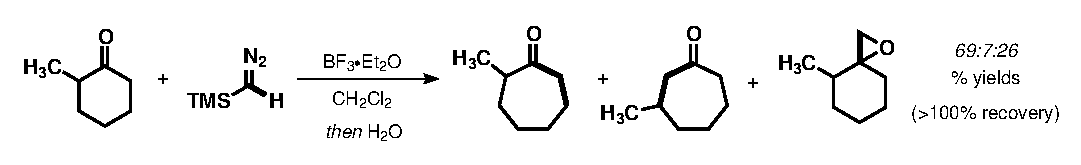
\includegraphics[scale=0.8]{chp_diazobkg/images/shioirione}
   \begin{textblock}{1}(2.2,0) \textsf{\scriptsize{\ref{cmp:aab}}}
 \end{textblock}
 \begin{textblock}{1}(9.9,0) \textsf{\scriptsize{\ref{cmp:aad}}}
 \end{textblock}
 \begin{textblock}{1}(12.7,0) \textsf{\scriptsize{\ref{cmp:aae}}}
 \end{textblock}
  \begin{textblock}{1}(15.8,0) \textsf{\scriptsize{\ref{cmp:aaf}}}
 \end{textblock}
   \begin{textblock}{1}(4.8,0) \textsf{\scriptsize{\ref{cmp:aaa}}}
 \end{textblock}
 \vspace{5pt}
  \caption{Use of trimethylsilyldiazomethane (TMSD) as an alternative to
  diazomethane.}
  \label{sch:shioiri}
\end{Scheme}

\begin{Scheme}[b]
  \centering 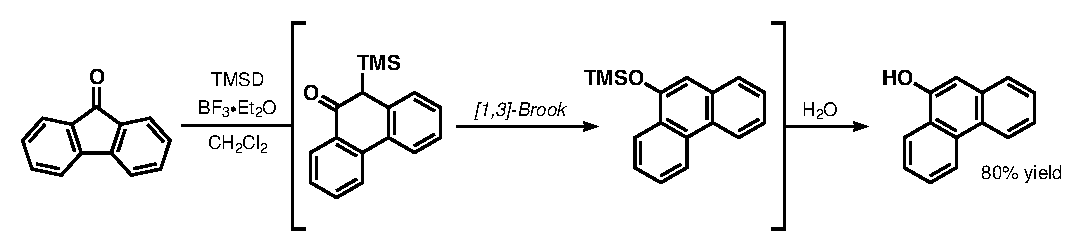
\includegraphics[scale=0.8]{chp_diazobkg/images/shioiritwo}
   \begin{textblock}{1}(1.65,-0.8) \cmp{aax} \end{textblock}
  \begin{textblock}{1}(7,-1) \cmp{aay} \end{textblock}
  \begin{textblock}{1}(13,-1) \cmp{aaz} \end{textblock}
  \begin{textblock}{1}(17.5,-0.5) \cmp{aba} \end{textblock}
  \caption{Facile 1,3-Brook rearrangement of $\alpha$-keto silane intermediate \ref{cmp:aay}.}
  \label{sch:shioiritwo}
\end{Scheme}
When
2-methylcyclohexanone (\ref{cmp:aab}, \refscheme{shioiri}) was treated with 1.5 equivalents of
\ce{BF3.Et2O} and 1.5 equivalents of TMSD (\ref{cmp:aaa}) in dichloromethane for 4 hours at $-$15
\degc, 2-- and 3-methylcycloheptanone (\ce{->}\ref{cmp:aad} + \ref{cmp:aae}) were produced with nearly 10:1
regioselectivity.
The 2-methyl regioisomer \ref{cmp:aad}, resulting from migration of the less substituted carbon, was
recovered in a 69\% yield.
This represents a marked improvement over Adamson and Kenner's previous efforts, which netted a 37\%
combined yield of 2-- and 3-methylcyclohexanone after 5 days with methanol as the
promoter.\footnote{No regioisomeric ratio was clearly reported, see reference
\ref{ref:adamsonkenner} for details.} The regioselectivity also agreed with previous reports in the
literature, showing an intrinsic preference for migration of the less substituted carbon regardless
of the promoter or diazoalkane.
When fluorenone (\ref{cmp:aax}, \refscheme{shioiritwo}) was subjected to the standard conditions,
the initially formed $\alpha$-keto silane \ref{cmp:aay} underwent facile Brook
rearrangement\footnote{Concerted 1,3-migration of silicon from carbon to oxygen. {\frenchspacing
Brook, A.
G.
Some Molecular Rearrangements of Organosilicon Compounds. \textit{Acc. Chem. Res.} \textbf{1974},
\textit{7}, 77-84.} \label{ref:brook}} to the aromatic silyl enol ether \ref{cmp:aaz}.
Refluxing in water afforded the deprotected phenol \ref{cmp:aba} in an overall 80\% yield. At the
time that TMSD was introduced, it was praised for its greater safety profile over diazomethane.
While it is true that TMSD has greater thermal
 stability and has since become commercially available, it should be regarded as highly toxic and
 great care must be exercised in its use.\footnote{For a note on the safety of TMSD see:
 {\frenchspacing Shioiri, T.; Aoyama, T.; Mori, S. Trimethylsilyldiazomethane. \textit{Org. Synth.}
 \textbf{1990}, \textit{68}, 1.}} At least two chemists were recently killed from lung failure after
 exposure to TMSD.\footnote{{\frenchspacing Kemsley, J. N. Firm Fined For Chemist's Death.
 \textit{Chem. Eng. News} \textbf{2011}, \textit{89}, 15.}}

\begin{Scheme}[b]
  \centering \includegraphics[scale=0.8]{chp_diazobkg/images/yamamotoone}
  \caption{Improved product distributions with aluminum-based Lewis acids.}
  %\begin{textblock}{1}(2.5,-7.8) \textsf{\scriptsize{\ref{cmp:aaa}}}
  %\begin{textblock}{1}(14,5.5) \cmp{mad} \end{textblock}
%\end{textblock}
  \label{sch:yamamotoone}
\end{Scheme}
Although the introduction of TMSD offered significant advantages over diazomethane based
homologations, there was still room to improve the product
distributions and discover more efficient promoters.
Yamamoto and
coworkers began to evaluate the efficacy of various aluminum-based Lewis acids.\footnote{(a)
\frenchspacing{Maruoka, K.; Concepcion, A. B.; Yamamoto, H. Selective Homologation of Ketones and Aldehydes with Diazoalkanes Promoted by Organoaluminum Reagents. \textit{Synthesis}. \textbf{1994}, 1283-1290}. (b) \frenchspacing{Maruoka, K.; Concepcion, A. B.; Yamamoto, H. Organoaluminum-Promoted Homologation of Ketones with Diazoalkanes. \textit{J.
Org. Chem.} \textbf{1994}, \textit{59}, 4725-4726.} \label{ref:yamamoto}}$^,$\footnote{An earlier
report by M\"uller and Bauer discussed the use AlCl$_3$. {\frenchspacing M\"uller, E.; Bauer, M.
Untersuchungen an Diazomethanen, XVI. Katalysierte Homologisierung cycloaliphatischer und
aliphatischer Ketone mit Diazoalkanen. \textit{Liebigs Ann. Chem.} \textbf{1962}, \textit{654}, 92-111.}} When cyclopentanone was treated with TMSD (\ref{cmp:aaa}) under Shioiri's standard conditions,\crossref{ref:shioiri} an overall 35\% yield was obtained with a poor product distribution (64\% cyclohexanone, 23\% cycloheptanone, 10\% cyclooctanone, 3\% epoxide).
By switching to trimethylaluminum (\refscheme{yamamotoone}), a substantially higher 68\% overall
yield was obtained with an improved product distribution (96\% cyclohexanone).
In a comparable manner to boron-based Lewis acids, alkylaluminum compounds were previously reported
to afford decomposition products when treated with diazomethane.\footnote{\frenchspacing{Hoberg, H.
Preparation and Rearrangement of Allylalanes.
\textit{Angew. Chem. Int. Ed.} \textbf{1966}, \textit{5}, 513-514.}\\
\includegraphics[scale=0.7]{chp_diazobkg/images/hoberg}} Yamamoto found that it was essential to
pre-mix the ketone and aluminum reagent for productive reactions to
occur.  



\begin{wrapfigure}{r}{1.45in}
  \vspace{-25pt}
  \begin{center}
    \includegraphics[scale=0.8]{chp_diazobkg/images/mad}
  \end{center}
  \begin{textblock}{1}(2.5,-1.5) \cmp{abb} \end{textblock}
  \vspace{-30pt}
\end{wrapfigure}
While trimethylaluminum was highly effective with TMSD (\refscheme{yamamotoone}), reactions with diazomethane afforded less desirable product distributions. To improve reaction efficiency and
broaden scope, Yamamoto began modifying the steric and electronic environment around the aluminum
center. When MAD (\ref{cmp:abb}) was utilized as the promoter,\footnote{Readily prepared \textit{in
situ} by pre-mixing trimethylaluminum and 2 equivalents of BHT. See reference \ref{ref:yamamoto}
for details.} excellent yields with minimal side products derived from overhomologation or
epoxidation were observed (\reftable{yamamoto}). Homologation of 4-\textit{tert}-butylcyclohexanone
(\ref{cmp:abc}) proceeded cleanly with MAD, affording a 95\% combined yield of all products with the desired singly homologated cycloheptanone \ref{cmp:abd} accounting
for 84\% of the recovered material (entry 4).
\begin{table}[h] \centering
\vspace{10pt}
\includegraphics[scale=0.8]{chp_diazobkg/images/yamamototable}
\begin{textblock}{1}(2.8,-2.2) \cmp{abc} \end{textblock}
\begin{textblock}{1}(7,-2.2) \cmp{abd} \end{textblock}
\begin{textblock}{1}(9,-2.2) \cmp{abe} \end{textblock}
\begin{textblock}{1}(11.5,-2.2) \cmp{abf} \end{textblock}
\begin{textblock}{1}(14,-2.2) \cmp{abg} \end{textblock}
\vspace{10pt}
{\footnotesize
\begin{tabular}{cccccc}
\toprule
entry & promoter & solvent & temp. (\degc) & yield (\%) &
\ref{cmp:abd}:\ref{cmp:abe}:\ref{cmp:abf}:\ref{cmp:abg}
\\
\midrule
1 & \ce{CH3OH} & \ce{Et2O} & 0 & 63 & 50 : 25 : 25 : 0 \\
2 & \textit{i}-Bu$_3$Al & \ce{CH2Cl2} & $-78$ & 68 & 54 : 22 : 22 : 2 \\
3 & \ce{(CH3)3Al} & \ce{CH2Cl2} & $-78$ & 70 & 66: 15 : 15 : 4 \\
4 & MAD (\ref{cmp:abb}) & \ce{CH2Cl2} & $-78$ & 95 & 84 : 3 : 3 : 10 \\ 
\bottomrule
\end{tabular}
}
\caption{Highly selective reactions with bulky aluminum Lewis acids.}
\label{tbl:yamamoto}
\end{table}


\begin{Scheme}[t]
  \centering 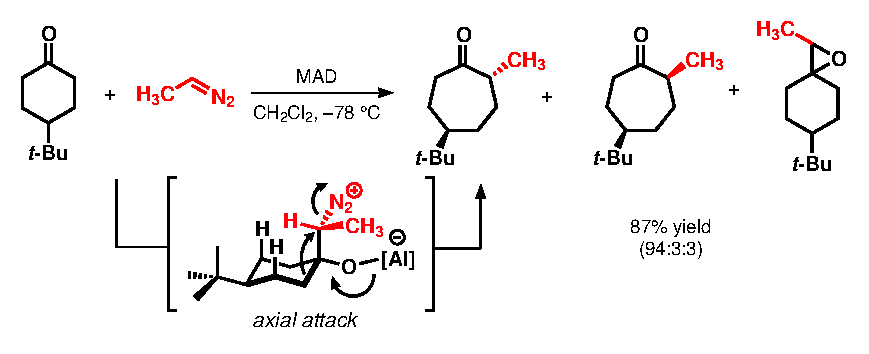
\includegraphics[scale=0.8]{chp_diazobkg/images/yamamotodiastereo}
  \caption{Diastereoselective insertion of diazoethane into 4-\textit{tert}-butylcyclohexanone.}
  \begin{textblock}{1}(1.6,-4) \textsf{\scriptsize{\ref{cmp:abc}}}
\end{textblock}
  \begin{textblock}{1}(5.1,-3.7) \cmp{abh} \end{textblock}
  \begin{textblock}{1}(10.5,-3.4) \cmp{abi} \end{textblock}
  \begin{textblock}{1}(14,-3.4) \cmp{abj} \end{textblock}
  %\begin{textblock}{1}(17.5,-4) \cmp{abk} \end{textblock}
  \begin{textblock}{1}(5.8,-2.6) \cmp{abl} \end{textblock}
  \label{sch:yamamotodiastereo}
\end{Scheme}
In an effort to further expand the reaction scope, Yamamoto and coworkers also explored
insertion reactions with a number of substituted diazoalkanes. With substituted diazoalkanes
and substrates containing an existing prochiral or stereogenic center, Yamamoto reported
some of the first diastereoselective diazo insertion reactions. When 4-\textit{tert}-butylcyclohexanone
(\ref{cmp:abc}) was combined with diazoethane (\ref{cmp:abh}) in the presence of 1.2 equivalents of
MAD (\ref{cmp:abb}), a highly efficient union produced predominantly the \textit{trans}-cycloheptanone
\ref{cmp:abi} in an isolated 82\% yield (87\% combined) with $>$30:1 diastereoselectivity
(\refscheme{yamamotodiastereo}).\footnote{The \textit{cis}/\textit{trans} configuration of 2-methyl-5-\textit{tert}-butylcycloheptanone was established by equilibration in methanolic
\ce{NaOCH3}.} The high diastereoselectivity may be accounted for by a model involving axial approach
of diazoethane in an orientation that places the diazo $\alpha$-proton over the six-membered ring
(\ref{cmp:abl}). A least motion collapse of the anti-periplanar \ce{C-C} bond, assuming no free
rotation once the diazoalkane has added, correctly predicts the major diastereomer. Applying the same analysis with an equatorial approach of the diazo
nucleophile leads to the minor \textit{cis} diastereomer (\ce{->}\ref{cmp:abj}). 


\subsection{Catalysis of Diazoalkane Ring Expansions}
Early work by House\crossref{ref:house} and Shiori\crossref{ref:shioiri} demonstrated that
diazoalkane insertion reactions may be effectively promoted by stoichiometric quantities of
\ce{BF3.Et2O}.
In Yamamoto's later work with aluminum-based Lewis acids, turnover was never
observed, presumably due to the high oxophilicity of aluminum.\crossref{ref:yamamoto} For over a
decade, Yamamoto's work would remain state of the art.\footnote{Johnson and coworkers observed some catalytic turnover with fluoroboric acid or boron trifluoride in the context of $\alpha$,$\beta$-unsatured ketone substrates. {\frenchspacing
Johnson, W. S.; Neeman, M.; Birkeland, S. P.; Fedoruk, N. A. The Acid-catalyzed Reaction of
Diazomethane with Some $\alpha$,$\beta$-Unsaturated Ketones. \textit{J. Am. Chem. Soc.} \textbf{1962}, \textit{84}, 989-992.}} Regardless of the lack of catalytic turnover, Yamamoto's work
illustrated some of the most selective and highest yielding diazoalkane ring expansion reactions recorded to date.


In 2006, work in the Kingsbury research group opened with a search for a broadly applicable and
catalytic non-stabilized diazoalkane ring expansion reaction.\footnote{{\frenchspacing Moebius, D.
C.; Kingsbury, J. S. Catalytic Homologation of Cycloalkanones with Substituted Diazomethanes. Mild
and Efficient Single-Step Access to $\alpha$-Tertiary and $\alpha$-Quaternary Carbonyl Compounds.
\textit{J. Am. Chem. Soc.} \textbf{2009}, \textit{131}, 878-879.} \label{ref:moebius}} A wide array
of potential aluminum-- and boron-based catalysts were evaluated first based on literature
precedents, but catalytic turnover was not observed in all cases
tested.\footnote{{\frenchspacing Moebius, D.
C.
Development of Sc(III)-Catalyzed Homologation of Ketones by Non-Stabilized Diazomethanes. Ph.D.
Dissertation, Boston College, Chestnut Hill, MA, 2011.}} A survey of potential H-bond donors
(alcohols, biphenols, diols, ureas, thioureas, etc\ldots) was also carried out, again with the same
discouraging results. A screen of lanthanide triflates was conducted and led to a highly rewarding
discovery. When cyclobutanone was exposed to phenyldiazomethane in the presence of 5 mol \%
\ce{Sc(OTf)3}, a rapid union occured to deliver the target compound 2-phenylcyclopentanone in a near
quantitative yield (\ce{->}\ref{cmp:abp}, \refscheme{moebius}). The new scandium-catalyzed reaction
also did not produce any of the common epoxide byproducts, but instead proceeded cleanly, producing
the desired product and nitrogen gas as the only stoichiometric byproduct.
At the time, no special precautions were taken to dry the commercial scandium salt, so a control
reaction was conducted to rule out protic catalysis. Exposure of cyclobutanone and
phenyldiazomethane to 1 mol \% triflic acid in toluene at 23 \degc\ did not produce any of the
desired homologation product, but instead lead exclusively to diazoalkane
decomposition.\footnote{The material recovered consisted of an approximately 1:1 \textit{E:Z}
mixture of stilbene.} \begin{Scheme}[p]
  \centering 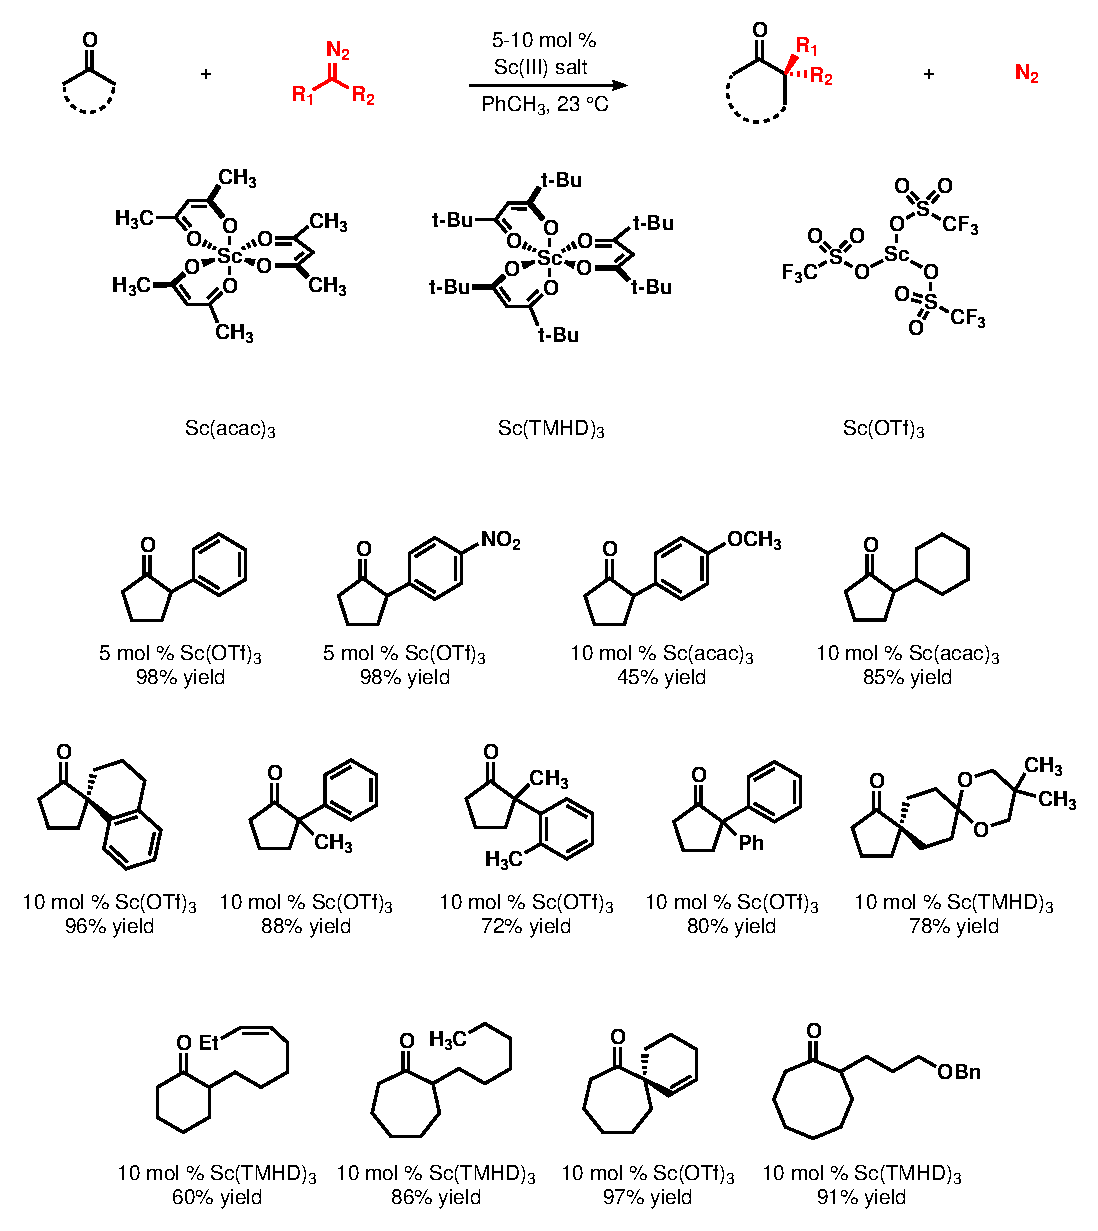
\includegraphics[scale=0.8]{chp_diazobkg/images/moebius}
  \vspace{10pt}
  \caption{Efficient catalysis of diazoalkane insertions with scandium (III) salts.}
 \begin{textblock}{1}(3.65,-15) \cmp{abm} \end{textblock}
 \begin{textblock}{1}(9.5,-15) \cmp{abn} \end{textblock}
 \begin{textblock}{1}(15.3,-15) \cmp{abo} \end{textblock}
 \begin{textblock}{1}(3.2,-11.1) \cmp{abp} \end{textblock}
 \begin{textblock}{1}(7.3,-11.1) \cmp{abq} \end{textblock}
 \begin{textblock}{1}(11.7,-11.1) \cmp{abr} \end{textblock}
  \label{sch:moebius}
\end{Scheme}


Pleased with this new discovery, the substrate scope with aryl-substituted diazoalkanes and
cyclobutanone was examined in greater detail. Steric modification of the diazoalkane was readily
tolerated, as both $\alpha$-tertiary and $\alpha$-quaternary centers were readily produced.
Switching to an electron poor aromatic (\textit{p}-\ce{NO2}) had little effect on the isolated yield
(\ce{->}\ref{cmp:abq}, 98\% yield). The more electron rich \textit{p}-OCH$_3$ susbstituted
diazoalkane required a less Lewis acidic \ce{Sc(acac)3} (\ref{cmp:abm}) catalyst and still afforded a diminished yield of
the product(\ce{->} \ref{cmp:abr}, 45\% yield).\footnote{Milder Lewis acids (\ref{cmp:abm} or
\ref{cmp:abn}) were substituted in reactions with more labile diazoalkanes because of the ability of Lewis acids to promote diazo
decomposition. See reference \ref{ref:yamamoto}a and references within for details.} The
\textit{p}-OCH$_3$ substituted phenyldiazomethane is highly unstable and known to decompose at temperatures as low as $-$80
\degc.\footnote{{\frenchspacing Fulton, J. R.; Aggarwal, V. K.; De Vicente, J. The Use of
Tosylhydrazone Salts as a Safe Alternative for Handling Diazo Compounds and Their Applications in
Organic Synthesis. \textit{Eur. J. Org. Chem.} \textbf{2005}, \textit{2005}, 1479-1492.}
\label{ref:aggarwal}} To further broaden the utility of the newly discovered scandium catalysis, an
examination of more reactive alkyl-substituted diazoalkanes was carried out. The highest yields were obtained with the weaker and
more sterically hindered Lewis acid \ce{Sc(TMHD)3} (\ref{cmp:abn}). Moderate to high yields were
obtained for a number of different ring sizes and diazo substitution patterns.


\begin{Scheme}[b]
  \centering
  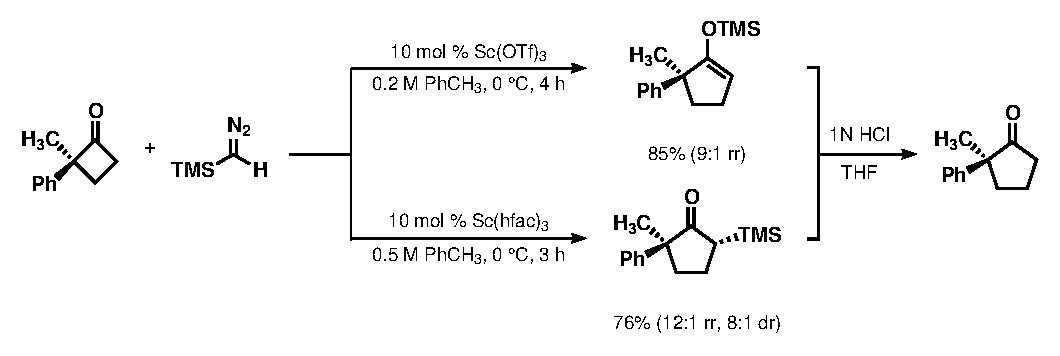
\includegraphics[scale=0.8]{chp_diazobkg/images/kingsburysingle}
  \caption{Regioselective scandium catalyzed single carbon ring expansion.}
  \begin{textblock}{1}(1.8,-2.5) \cmp{abs} \end{textblock}
 \begin{textblock}{1}(12.6,-4) \cmp{abt} \end{textblock}
 \begin{textblock}{1}(12.4,-1) \cmp{abu} \end{textblock}
 \begin{textblock}{1}(18.1,-2.5) \cmp{abv} \end{textblock}
  \begin{textblock}{1}(4.2,-2.5) \textsf{\scriptsize{\ref{cmp:aaa}}}
  \end{textblock}
  \label{sch:kingsburysingle}
\end{Scheme}
The substrates first
tested under catalytic conditions were all symmetrical cycloalkanones. In a subsequent report,
differentially substituted cycloalkanones were examined in the context of regioselective single-carbon homologations (\refscheme{kingsburysingle}).\footnote{{\frenchspacing Dabrowski, J.
A.; Moebius, D.
C.; Wommack, A. J.; Kornahrens, A. F.; Kingsbury, J. S. Catalytic and Regioselective Ring Expansion
of Arylcyclobutanones with Trimethylsilyldiazomethane. Ligand-Dependent Entry to $\beta$-Ketosilane
or Enolsilane Adducts. \textit{Org. Lett.} \textbf{2010}, \textit{12}, 3598-3601.}} When
$\alpha$,$\alpha$-disubstituted cyclobutanone \ref{cmp:abs} was treated with TMSD in the presence of
10 mol \% scandium triflate, silyl enol ether \ref{cmp:abt} was obtained in an 85\% isolated yield as a single compound (9:1
regioselectivity from crude $^1$H NMR spectroscopy). In constrast to previously discussed methods,
the intermediate silyl enol ether could be purified by chromatography and isolated, providing access
to a synthetically useful functional handle. Dilute acid hydrolysis in THF delivered the
cyclopentanone \ref{cmp:abv} in high yield.
 Monitoring of the reaction \textit{in situ} with ReactIR
revealed a dual role for \ce{Sc(OTf)3}, first catalyzing a rapid insertion of TMSD to produce
\ref{cmp:abu}. The initial insertion product was then gradually converted to \ref{cmp:abt} through
a 1,3-Brook\crossref{ref:brook} rearrangement.
By switching the catalyst to the milder \ce{Sc(hfac)3}, the reaction was effectively terminated at
\ref{cmp:abu}, allowing the $\beta$-keto silane to be isolated in a 76\% yield. 
 
The seminal report from the Kingsbury group in 2009\crossref{ref:moebius} disclosed the first
\textit{catalytic} ring expansion reactions with substituted diazoalkanes.\footnote{The Maruoka
group reported substoichiometric carbonyl-stabilized diazoalkane insertion reactions with boron and
aluminum Lewis acids around the same time. (a) {\frenchspacing Hashimoto, T.; Naganawa, Y.; Maruoka,
K.
Stereoselective Construction of Seven-Membered Rings with an All-Carbon Quaternary Center by Direct
Tiffeneau--Demjanov-type Ring Expansion. \textit{J. Am. Chem. Soc.} \textbf{2009}, \textit{131},
6614-6617.} (b) {\frenchspacing Hashimoto, T.; Naganawa, Y.; Maruoka, K. Desymmetrizing Asymmetric
Ring Expansion of Cyclohexanones with $\alpha$-Diazoacetates Catalyzed by Chiral Aluminum Lewis
Acid. \textit{J. Am. Chem. Soc.} \textbf{2011}, \textit{133}, 8834-8837.}} Subsequent studies
showed that the new conditions were amenable to regioselective single-carbon ring expansions, as
well as regioselective aldehyde homologations.\footnote{{\frenchspacing Wommack, A. J.; Moebius, D.
C.; Travis, A. L.; Kingsbury, J. S. Diverse Alkanones by Catalytic Carbon Insertion into the Formyl
C-H Bond. Concise Access to the Natural Precursor of Achyrofuran. \textit{Org. Lett.} \textbf{2009},
\textit{11}, 3202-3205.}} The new scandium-catalyzed reactions offered significant advantages over previous methods.
Not only were the reactions catalytic, the conditions were milder and the product distributions were more favorable. Ring expansion products could be obtained in relatively short reaction
times and in high yields with high levels of regiocontrol. 

\pagebreak
%%%%%%%%%%%%%%%%%%%%%%%%%%%%%%%%%%%%%%%%%%%%%%%%%%%%%%%%%%%%%%%%%%%%%%%%%%%%%%%%%%%%%%%%%%%%%%%%%%
%%%%%%%%%%%%%%%%%%%%%%%%%%%%%%%%%%%%%%%%%%%%%%%%%%%%%%%%%%%%%%%%%%%%%%%%%%%%%%%%%%%%%%%%%%%%%%%%%%
%%%%%%%%%%%%%%%%%%%%%%%%%%%%%%%%%%%%%%%%%%%%%%%%%%%%%%%%%%%%%%%%%%%%%%%%%%%%%%%%%%%%%%%%%%%%%%%%%%

\section{Conclusion and Outlook}

While the hazards of diazoalkanes may deter many chemists from using these powerful reagents, work
is already underway to find creative ways of generating these compounds for use \textit{in
situ}.\footnote{For lead references see reference \ref{ref:aggarwal} and {\frenchspacing Kirmse, W.
Reactive Intermediates from \textit{N}-Aziridinylimines. \textit{Eur. J. Org. Chem.} \textbf{1998},
\textit{1998}, 201-212.}} As methodologies mature and their potential is realized, chemists will no longer be able to ignore diazoalkanes when thinking about strategies to access new molecules. Ring expansion of ketones is only one small area where diazoalkanes find use, and significant advances have been made over the
past 125 years. Someday chemists may be able to insert a fully substituted carbon atom adjacent a
carbonyl with complete regio-- and stereochemical control using exceptionally low catalyst loadings.
In the two chapters that follow, further advances to ring expansion chemistry are presented that begin
to address that ultimate goal. Chapter \ref{chp:asymmetric} will discuss progress made toward the
development of a highly enantioselective homologation reaction with monoarylated diazomethanes.
Chapter \ref{chp:singlecarbon} presents advances made with regioselective single-carbon methylene
insertion that now allow catalytic reactions to be performed on complex targets with
regioselectivities of $>$20:1 in certain cases.
\pagebreak
%%%%%%%%%%%%%%%%%%%%%%%%%%%%%%%%%%%%%%%%%%%%%%%%%%%%%%%%%%%%%%%%%%%%%%%%%%%%%%%%%%%%%%%%%%%%%%%%%%
%%%%%%%%%%%%%%%%%%%%%%%%%%%%%%%%%%%%%%%%%%%%%%%%%%%%%%%%%%%%%%%%%%%%%%%%%%%%%%%%%%%%%%%%%%%%%%%%%%
%%%%%%%%%%%%%%%%%%%%%%%%%%%%%%%%%%%%%%%%%%%%%%%%%%%%%%%%%%%%%%%%%%%%%%%%%%%%%%%%%%%%%%%%%%%%%%%%%%
%%% Reset counters for the footnotes and compound numbering
%\setcounter{compound}{0}
\stepcounter{cmpreset}
\captionsetup[figure]{list=no} % hide figures from list in experimental section

\chapter{Development of Sc(III)-Catalyzed Asymmetric Homologation of\\
 Cycloalkanones with Non-Stabilized Diazoalkanes}
 \label{chp:asymmetric}
 %\thispagestyle{empty}
 \pagebreak
 
 \section{Introduction}
 \doublespacing
 
 In previous work, we had
 demonstrated that scandium (III) salts function as highly effective catalysts for the diazoalkane carbonyl homologation reaction.\footnote{See chapter \ref{chp:diazobkg} for a more thorough discussion. (a) {\frenchspacing Moebius, D. C.; Kingsbury, J. S. Catalytic Homologation of Cycloalkanones with Substituted Diazomethanes. Mild and Efficient
 Single-Step Access to $\alpha$-Tertiary and $\alpha$-Quaternary Carbonyl Compounds. \textit{J. Am. Chem. Soc.} \textbf{2009}, \textit{131}, 878-879.} (b) {\frenchspacing
 Wommack, A. J.; Moebius, D. C.; Travis, A. L.; Kingsbury, J. S. Diverse Alkanones by Catalytic
 Carbon Insertion into the Formyl C-H Bond. Concise Access to the Natural Precursor of Achyrofuran.
 \textit{Org. Lett.} \textbf{2009}, \textit{11}, 3202-3205.} (c) {\frenchspacing Dabrowski, J. A.;
 Moebius, D. C.; Wommack, A. J.; Kornahrens, A. F.; Kingsbury, J. S. Catalytic and Regioselective
 Ring Expansion of Arylcyclobutanones with Trimethylsilyldiazomethane. Ligand-Dependent Entry to
 $\beta$-Ketosilane or Enolsilane Adducts. \textit{Org. Lett.} \textbf{2010}, \textit{12},
 3598-3601.} \label{ref:askingsbury}} Given the success of these early reactions, we were eager to
 begin developing a general catalytic enantioselective version of the reaction. In the ideal transformation, a generic
 ketone, when combined with a chiral scandium catalyst and diazoalkane would undergo a regio-- and
 stereoselective union to deliver a new homologated ketone (\ce{->}\ref{cmp:asaaa}, \refscheme{generalrxn}).
 We believed it would be logical to start by extending the ring expansion of symmetrical
 cycloalkanones to stereoselective insertion reactions.\footnote{{\frenchspacing Rendina, V. L.;
 Moebius, D. C.; Kingsbury, J. S. An Enantioselective Synthesis of 2-Aryl Cycloalkanones by
 Sc-Catalyzed Carbon Insertion. \textit{Org. Lett.} \textbf{2011}, \textit{13}, 2004-2007.}} 
  \begin{Scheme}[h]
  \centering \includegraphics[scale=0.8]{chp_asymmetric/images/generalrxn}
  \begin{textblock}{1}(12.7,-4.1) \cmp{asaaa} \end{textblock}
  \caption{General catalytic regio-- and enantioselective diazoalkane insertion.}
  \label{sch:generalrxn}
\end{Scheme}   
 By starting from symmetrical cycloalkanones of the appropriate ring size,\footnote{The
 order of reactivity for the ring expansion of cycloalkanones with diazomethane based on literature
 precedents and qualitative observations is: cyclobutanone $\approx$ cyclohexanone $>$
 cycloheptanone $>$ cyclopentanone. \frenchspacing{Gutsche, C.
D. The Reaction of Diazomethane and Its Derivatives with Aldehydes and Ketones.
\textit{Org. React.} \textbf{1954}, \textit{8}, 364-403}. \label{ref:asgutscherev}} the classic
problems of regiochemical control could be removed and issues with overhomologation could be
minimized initially.
The ultimate goal of the project was to develop general methods for the construction alkyl, vinyl, and aryl
 bearing stereogenic centers adjacent to the carbonyl functionality.

 
%   \begin{figure}[h]
%   \centering
%   \vspace{2.8in}
%   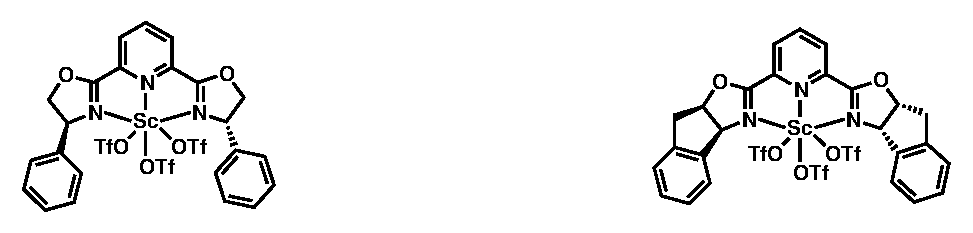
\includegraphics[scale=0.8]{chp_asymmetric/images/evanspybox}
%   \begin{textblock}{5}(-1,-4) \small \textsf{\textit{Evans}
%   \textbf{2001}\crossref{ref:asevans}\textsuperscript{a}}\end{textblock}
%   \begin{textblock}{5}(10,-4) \small \textsf{\textit{Evans}
%   \textbf{2003}\crossref{ref:asevans}\textsuperscript{b}}\end{textblock}  
%   \begin{textblock}{1}(0,-12)
%   \includegraphics[scale=0.35]{chp_asymmetric/images/evanspybox2ortep}\end{textblock}
%   \begin{textblock}{1}(10.5,-13)
%   \includegraphics[scale=0.4]{chp_asymmetric/images/evanspyboxortep}\end{textblock}
%   \caption{Crystal structures of Evan's pybox \ce{Sc(OTf)3} complexes.}
%   \label{fig:evanspybox}
%   \end{figure}  
%  
 We felt confident that by combining scandium (III) salts with the correct chiral ligand, the
 catalyst ligand complex would efficiently direct the stereochemical outcome of the newly forged
 \ce{C-C} bonds. A survey of the Cambridge Structural Database\footnote{{\frenchspacing
 Cambridge Structural Database (WebCSD). http://webcsd.ccdc.cam.ac.uk.proxy.bc.edu (accessed Jan 25, 2013).}} revealed
 four crystal structures containing chiral ligands bound to scandium triflate.
 Among the most well characterized and widely studied are the scandium PyBOX complexes reported by
 the Evans' group (\ref{cmp:asaaaa} and \ref{cmp:asaaab}, \reffigure{xraypage}).\footnote{ (a)
 {\frenchspacing Evans, D.
 A.; Sweeney, Z.
 K.; Rovis, T.; Tedrow, J. S. Highly Enantioselective Syntheses of Homopropargylic Alcohols and Dihydrofurans Catalyzed by a Bis(oxazolinyl)pyridine--Scandium Triflate Complex. \textit{J. Am. Chem. Soc.} \textbf{2001},
 \textit{123}, 12095-12096.} (b) {\frenchspacing Evans, D. A.; Scheidt, K. A.; Fandrick, K. R.; Lam,
 H. W.; Wu, J. Enantioselective Indole Friedel-Crafts Alkylations Catalyzed by
 Bis(oxazolinyl)pyridine--Scandium(III) Triflate Complexes. \textit{J. Am. Chem. Soc.}
 \textbf{2003}, \textit{125}, 10780-10781.} \label{ref:asevans}} Both structures show scandium bound
 with an additional water molecule (omitted from the line drawings for clarity), bringing the
 coordination number to seven.
 Two additional scandium triflate structures, one based on a proline-derived
 \textit{N}-oxide ligand (\ref{cmp:asaaac})\footnote{{\frenchspacing Liu, Y.;
 Shang, D.; Zhou, X.; Liu, X.; Feng, X. Enantioselective Friedel-Crafts Alkylation of Indoles with
 Alkylidene Malonates Catalyzed by \textit{N},\textit{N}-Dioxide-Scandium(III) Complexes:
 Asymmetric Synthesis of $\beta$-Carbolines. \textit{Chem. Eur. J.} \textbf{2009}, \textit{15},
 2055-2058.} \label{ref:asfengstructure}} and one based on a BINOL ligand
 framework\footnote{{\frenchspacing Di Bari, L.; Di Pietro, S.; Pescitelli, G.; Tur, F.; Mansilla,
 J.; Sa\'{a}, J. M. \ce{[Ln(binolam)3].(OTf)3}, a New Class of Propeller-Shaped Lanthanide(III) Salt
 Complexes as Enantioselective Catalysts: Structure, Dynamics and Mechanistic Insight. \textit{Chem.
 Eur. J.} \textbf{2010}, \textit{16}, 14190-14201.}} were reported in 2009 and 2010, respectively. A
 wider search revealed a fifth chiral scandium complex, containing \ce{ScBr3} complexed with a
 bipyridine-based ligand (\ref{cmp:asaaad}).\footnote{{\frenchspacing Ishikawa,
 S.; Hamada, T.; Manabe, K.; Kobayashi, S.
 Catalytic Asymmetric Hydroxymethylation of Silicon Enolates Using an Aqueous Solution of Formaldehyde with a Chiral Scandium Complex. \textit{J. Am. Chem. Soc.}
 \textbf{2004}, \textit{126}, 12236-12237.} \label{ref:askobayashistructure}} 
 
  \begin{figure}[p]
  \centering
  \vspace{1.6in}
  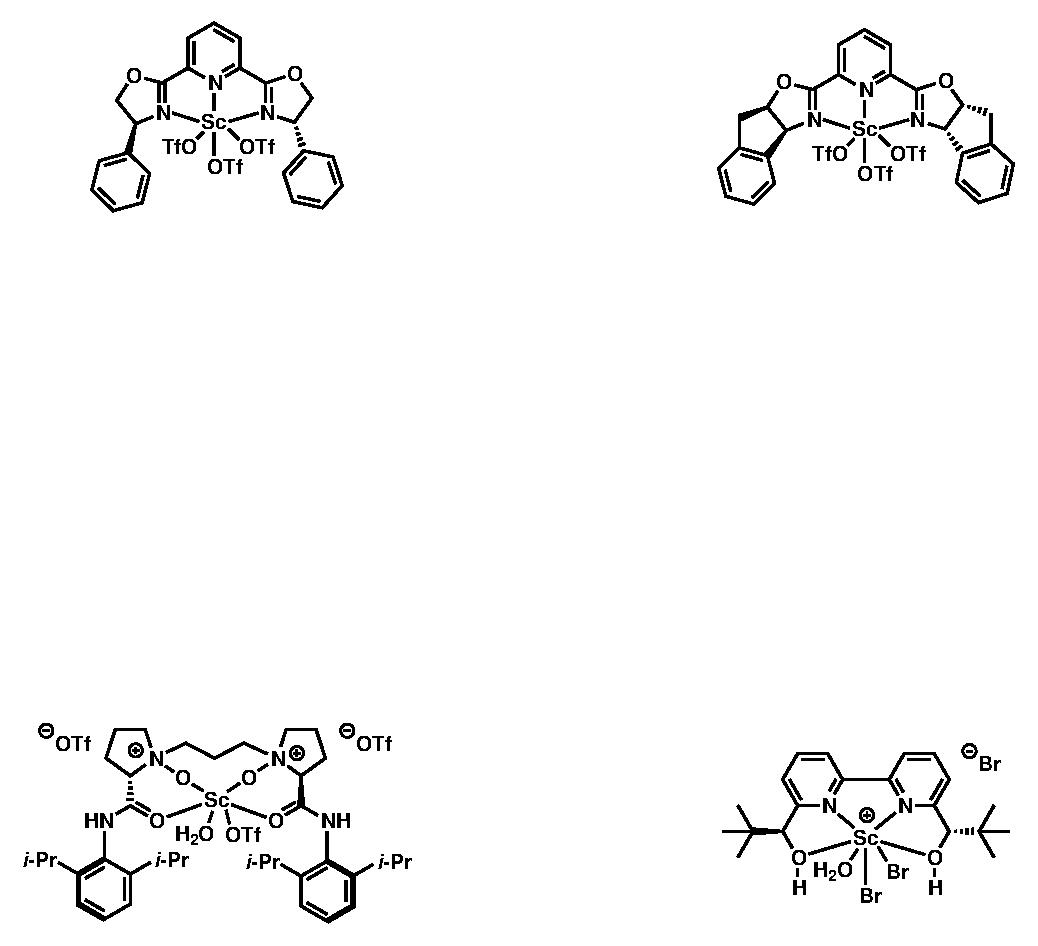
\includegraphics[scale=0.8]{chp_asymmetric/images/xraypage}
  %%%%% references
  \begin{textblock}{5}(2,-12.5) \small \textsf{\textit{Evans}
  \textbf{2001}\crossref{ref:asevans}\textsuperscript{a}}\end{textblock}
  \begin{textblock}{5}(14,-12.5) \small \textsf{\textit{Evans}
  \textbf{2003}\crossref{ref:asevans}\textsuperscript{b}}\end{textblock}
    \begin{textblock}{5}(2.1,0) \small \textsf{\textit{Feng}
   \textbf{2009}\crossref{ref:asfengstructure}}\end{textblock}
   \begin{textblock}{5}(14,0) \small \textsf{\textit{Kobayashi}
   \textbf{2004}\crossref{ref:askobayashistructure}}\end{textblock} 
   %%%% compound numbers
   \begin{textblock}{1}(1.5,-15) \cmp{asaaaa} \end{textblock}
   \begin{textblock}{1}(13.5,-15.5) \cmp{asaaab} \end{textblock}
   \begin{textblock}{1}(0.5, -2.5) \cmp{asaaac} \end{textblock}
   \begin{textblock}{1}(13,-3) \cmp{asaaad} \end{textblock}
   %%%% crystal structures
   \begin{textblock}{1}(0,-24.5)
   \includegraphics[scale=0.35]{chp_asymmetric/images/evanspybox2ortep}\end{textblock}
   \begin{textblock}{1}(10.5,-25.5)
   \includegraphics[scale=0.4]{chp_asymmetric/images/evanspyboxortep}\end{textblock}
   \begin{textblock}{1}(10,-11.5)
   \includegraphics[scale=0.3]{chp_asymmetric/images/kobayashibromideortep}\end{textblock}
    \begin{textblock}{1}(-1,-12.5)
  \includegraphics[scale=0.35]{chp_asymmetric/images/fengoxideortep}\end{textblock}
  \vspace{0.3in}
  \caption{Crystal structures of selected chiral scandium complexes.}
  \label{fig:xraypage}
  \end{figure}
 
 Three of the four
 structures in \reffigure{xraypage} contain a seven
 coordinate pentagonal bipyramidal metal geometry. Scandium (III), because of its filled valence shell
 and lack of \textit{d} electrons, tends to adopt coordination geometries that are based primarily
 on steric constraints rather than traditional orbital overlap based geometries
 observed for the transition metals.\footnote{{\frenchspacing Wu, J. Enantioselective
 Lanthanide-Catalyzed Mukaiyama Aldol, Carbonyl-Ene, Sakurai-Hosomi, and Quinone Diels-Alder Reactions. Ph.D. Dissertation, Harvard University, Cambridge, MA, 2005.} } The
 literature clearly shows precedents for scandium to form well-defined and competent chiral
 catalysts. Chiral scandium complexes have been used to
 catalyze a number of asymmetric \ce{C-C} bond forming reactions.\footnote{For reviews see: (a) {\frenchspacing Kobayashi, S.
 Scandium Triflate in Organic Synthesis. \textit{Eur. J. Org. Chem.} \textbf{1999}, 15-27.} (b)
 {\frenchspacing Mikami, K.; Terada, M.; Matsuzawa, H.
 ``Asymmetric'' Catalysis by Lanthanide Complexes. \textit{Angew. Chem. Int. Ed.} \textbf{2002},
 \textit{41}, 3512-3554.} (c) {\frenchspacing Kobayashi, S.; Sugiura, M.; Kitagawa, H.; Lam, W. W.
 L. Rare-Earth Metal Triflates in Organic Synthesis. \textit{Chem. Rev.} \textbf{2002},
 \textit{102}, 2227-2302.}} 
 


 
%  \begin{figure}[h]
%   \centering
%   \vspace{2.5in}
%   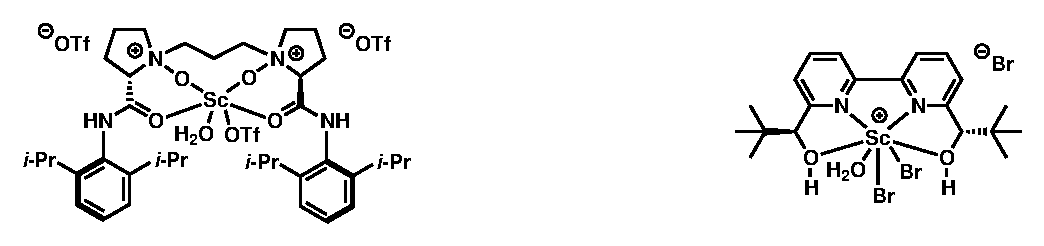
\includegraphics[scale=0.8]{chp_asymmetric/images/fengkobxrays}
%   \begin{textblock}{5}(2.1,0) \small \textsf{\textit{Feng}
%   \textbf{2009}\crossref{ref:asfengstructure}}\end{textblock}
%   \begin{textblock}{5}(14,0) \small \textsf{\textit{Kobayashi}
%   \textbf{2004}\crossref{ref:askobayashistructure}}\end{textblock}  
%   \begin{textblock}{1}(-1,-13)
%   \includegraphics[scale=0.6]{chp_asymmetric/images/fengoxideortep}\end{textblock}
%   \begin{textblock}{1}(10,-11.5)
%   \includegraphics[scale=0.35]{chp_asymmetric/images/kobayashibromideortep}\end{textblock}
%   \vspace{20pt}
%   \caption{Crystal structures of chiral scandium complexes.}
%   \label{fig:fengkobxrays}
%   \end{figure}  
  
  In the sections that follow, an account of how we developed the first catalytic asymmetric
  diazoalkane carbon insertion reactions is presented. The crystallographic data from the literature
  suggests a logical starting point for the development of a new method based on chiral scandium complexes. Ligand constructs
 known to form competent catalysts with Sc(III) salts would be among the first screened for
 asymmetric induction. Before discussing
  experimental details, a brief background on alternative methods for the synthesis of
  $\alpha$-substituted cycloalkanones is given. 
 
 \pagebreak
 \section{Methods for Asymmetric $\alpha$-Functionalization of
 Cycloalkanones}
 
 \subsection{Construction of $\alpha$-Tertiary Centers}
 
 One of the most common methods for \ce{C-C} bond construction involves the
 $\alpha$-functionalization of ketone enolates.
 Some of the first sucessful methods for $\alpha$-functionalized of cycloalkanes in a
 stereocontrolled fashion relied extensively on the pre-formation of chiral imines or hydrazones. In
 1976, Meyers and coworkers reported a highly enantioselective synthesis of 2-alkyl substituted
 cyclohexanones through the formation of a lithio-chelated enamine
 nucleophile (\ref{cmp:asaab}, \refscheme{asmeyers}).\footnote{{\frenchspacing Meyers, A. I.;
 Williams, D.
 R.; Druelinger, M.
 Enantioselective Alkylation of Cyclohexanone via Chiral Lithio-Chelated Enamines. \textit{J. Am.
 Chem. Soc.} \textbf{1976}, \textit{98}, 3032-3033.}} Upon treatment with an alkyl electrophile,
 a stereoselective trap of the electrophile lead to products in up to 97.5:2.5 er
 after careful imine hydrolysis.
 The introduction of a chelating methyl ether moiety rigidified the proposed metalloenamine
 intermediate \ref{cmp:asaab} and led to much higher levels of stereocontrol than previous reports
 with imines that lacked an additional chelating group.\footnote{(a) {\frenchspacing Mea-Jacheet, D.; Horeau, A. Asymmetric Synthesis and Optical purity of 2-Methylcyclohexanone. \textit{Bull. Soc. Chim. Fr.} \textbf{1968}, 4571-4573.} (b) {\frenchspacing Kitamoto, M.; Hiroi, K.; Terashima, S.
 Stereochemical Studies. XXIX. Asymmetric Synthesis of 2-Alkylcyclohexanones via Optically Active
 Lithioenamines. \textit{Chem. Pharm. Bull.} \textbf{1974}, \textit{22}, 459-464.}} 
  \begin{Scheme}[h]
  \centering
  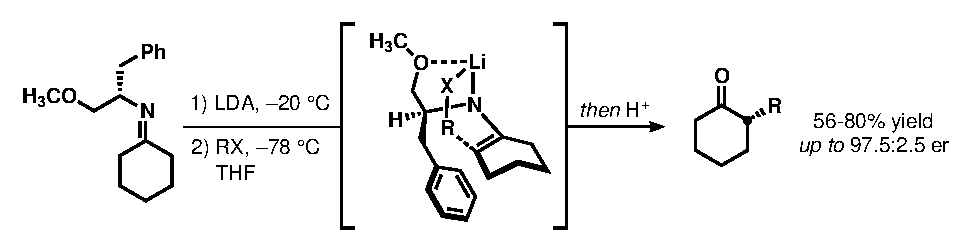
\includegraphics[scale=0.8]{chp_asymmetric/images/meyers}
  \begin{textblock}{1}(7.8,-1) \cmp{asaab} \end{textblock}
  \caption{Meyers auxiliary based approach for $\alpha$-alkylation.}
  \label{sch:asmeyers}
\end{Scheme}   
 
 Around the time of Meyers work, the Enders group introduced the proline derived chiral auxiliary
 (\textit{S})-1-amino-2-methoxymethylpyrrolidine (SAMP, \ref{cmp:asaad}, \refscheme{assamp}), which
 contained a very similar chelating functional group.\footnote{{\frenchspacing Enders, D.; Eichenauer, H.
 Asymmetric Synthesis of $\alpha$-Substituted Ketones by Metalation and Alkylation of Chiral Hydrazones. \textit{Angew.
 Chem. Int. Ed.} \textbf{1976}, \textit{15}, 549-551.}} The SAMP auxiliary and related derivatives
 have been widely utilized for their often very high and predictable levels of stereoinduction and
 for their mild and varied means of cleavage.\footnote{For a recent review see: {\frenchspacing Job, A.; Janeck, C. F.; Bettray, W.;
 Peters, R.; Enders, D. The SAMP-/RAMP-Hydrazone Methodology in Asymmetric Synthesis.
 \textit{Tetrahedron} \textbf{2002}, \textit{58}, 2253-2329.}} In the context of a cycloheptanone
 substrate, the Holmes group sucessfully applied a SAMP hydrazone alkylation strategy to their
 enantioselective synthesis of ($-$)-gloeosporone
 (\ce{->}\ref{cmp:asaac}, \refscheme{assamp}).\footnote{{\frenchspacing Curtis, N.
 R.; Holmes, A. B.; Looney, M. G.; Pearson, N. D.; Slim, G. C. Synthesis of ($-$)-Gloeosporone.
 \textit{Tetrahedron Lett.} \textbf{1991}, \textit{32}, 537-540.}} Cleavage of the auxiliary was
 achieved by treatment with ozone at low temperature, delivering the target cycloheptanone
 \ref{cmp:asaaca} in 97:3 er. 
 \begin{Scheme}[t]
  \centering
  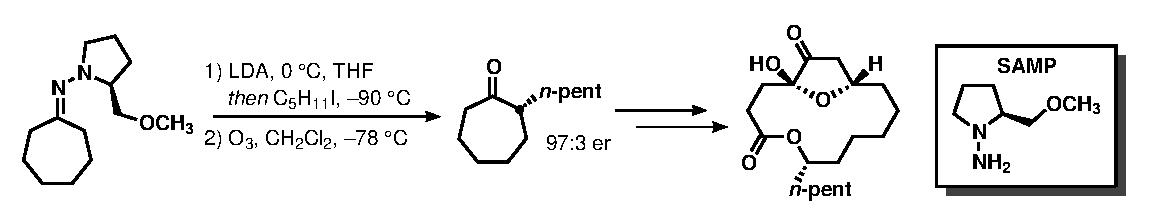
\includegraphics[scale=0.8]{chp_asymmetric/images/samp}
  \begin{textblock}{1}(8.5,-0.5) \cmp{asaaca} \end{textblock}
  \begin{textblock}{1}(15,-1) \cmp{asaac} \end{textblock}
  \begin{textblock}{1}(18,-1) \cmp{asaad} \end{textblock}
  \caption{Application of Ender's SAMP auxiliary in total synthesis.}
  \label{sch:assamp}
\end{Scheme}   
 
More modern strategies have focused on the use of chiral catalysts to control stereochemistry, which
foregoes the need to pre-install a costly chiral auxiliary in the substrate. The formation of an
$\alpha$-tertiary center requires control over either the installation of the $\alpha$-substituent
through an asymmetric alkylation event or control over installation of the $\alpha$-hydrogen. Aside
from stoichiometric auxiliary-based approaches, catalytic methods for enolate alkylation based on
phase transfer catalysts\footnote{{\frenchspacing Dolling, U. H.; Davis, P.; Grabowski, E. J. J.
Efficient Catalytic Asymmetric Alkylations. 1. Enantioselective Synthesis of (+)-Indacrinone
\textit{via} Chiral Phase-Transfer Catalysis. \textit{J. Am. Chem. Soc.} \textbf{1984}, \textit{106}, 446-447.}} and chiral lithium enolates\footnote{{\frenchspacing Imai, M.; Hagihara, A.; Kawasaki, H.; Manabe, K.; Koga, K. Catalytic Asymmetric Benzylation of Achiral Lithium Enolates Using a Chiral Ligand for Lithium in the Presence of an Achiral Ligand. \textit{J. Am. Chem. Soc.}
\textbf{1994}, \textit{116}, 8829-8830.}} have also been demonstrated. Alternative approaches have
examined catalytic methods for the installation of an $\alpha$-hydrogen through an enantioselective
enolate protonation event.\footnote{For a review see:
{\frenchspacing Mohr, J.
T.; Hong, A.
Y.; Stoltz, B.
M.
Enantioselective Protonation. \textit{Nature Chem.} \textbf{2009}, \textit{1}, 359-369.}} Achieving
stereocontrol while delivering a group as small as a proton has been a significant challenge and
the subject of considerable research.
 
In 2005, the Yanagisawa group introduced an asymmetric protonation method utilizing a simple
catalyst system derived from commercially available silver fluoride and (\textit{R})-BINAP.\footnote{{\frenchspacing Yanagisawa, A.; Touge, T.; Arai, T.
Enantioselective Protonation of Silyl Enolates Catalyzed by a
\ce{Binap.AgF} Complex. \textit{Angew. Chem. Int. Ed.} \textbf{2005}, \textit{44}, 1546-1548.}
\label{ref:asyanagisawa}} Starting from a pre-formed silyl enol ether, face selective delivery of
the proton from methanol was proposed to proceed through a silver fluoride BINAP complex that delivered methanol while
concomitantly deprotecting the silyl ether (\ref{cmp:asaae}, \refscheme{asyanagisawaproton}). High
yields and near perfect enantioselectivities were observed across a range of 2-aryl substituted cyclic substrates. The
Yamamoto group also demonstrated a very similar asymmetric protonation reaction with a comparable
substrate scope using a non-commercial chiral phosphoric acid catalyst.\footnote{{\frenchspacing
Cheon, C.
H.; Yamamoto, H.
A Br\o nsted Acid Catalyst for the Enantioselective Protonation Reaction. \textit{J. Am. Chem. Soc.}
 \textbf{2008}, \textit{130}, 9246-9247.}}  
\begin{Scheme}[h]
  \centering
  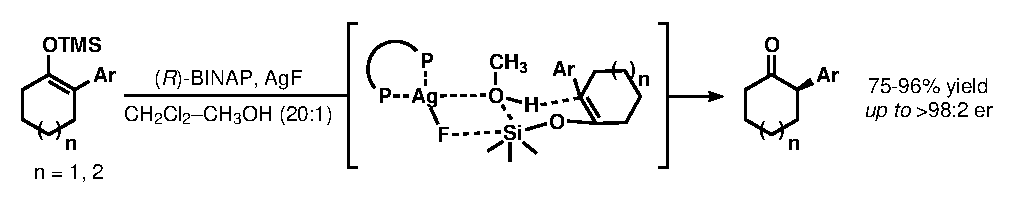
\includegraphics[scale=0.8]{chp_asymmetric/images/yanagisawaproton}
  \begin{textblock}{1}(11,-0.5) \cmp{asaae} \end{textblock}
  \caption{Yanagisawa's asymmetric protonation of silyl enol ethers.}
  \label{sch:asyanagisawaproton}
\end{Scheme}  
 
 
 
 The Stoltz group has also examined enantioselective protonation reactions in the context
 of palladium enolates.\footnote{(a) {\frenchspacing Mohr, J. T.; Nishimata, T.; Behenna, D.
 C.; Stoltz, B.
 M.
 Catalytic Enantioselective Decarboxylative Protonation. \textit{J. Am. Chem. Soc.} \textbf{2006},
 \textit{128}, 11348-11349.} (b) {\frenchspacing Marinescu, S. C.; Nishimata, T.; Mohr, J. T.;
 Stoltz, B. M.
 Homogeneous Pd-Catalyzed Enantioselective Decarboxylative Protonation. \textit{Org. Lett.}
 \textbf{2008}, \textit{10}, 1039-1042.} \label{ref:stoltzprotonation}} When a racemic allyl
 $\beta$-ketoester (\ref{cmp:asaaf}, \refscheme{asstoltzprotonation}) is combined with Pd(0) in the presence of
 PHOX ligand \ref{cmp:asaah}, oxidative addition to the allyl group followed by decarboxylation
 furnishes a chiral palladium enolate intermediate. By adding a superstoichiometric amount of
 Meldrum's acid (\ref{cmp:asaag}, 2.5 equiv), the reaction can be effectively interrupted before
 reductive elimination to deliver $\alpha$-tertiary substituted cycloalkanones in high yields and enantioselectivities. The catalytic cycle is closed by ultimately delivering the allyl fragment to the Meldrum's acid enolate, regenerating the
 Pd(0) catalyst.
  \begin{Scheme}[h]
  \centering
  \includegraphics[scale=0.8]{chp_asymmetric/images/stoltzprotonation}
  \begin{textblock}{1}(1.5,-1.5) \cmp{asaaf} \end{textblock}
  \begin{textblock}{1}(4.9,-1.5) \cmp{asaag} \end{textblock}
  \begin{textblock}{1}(16,-1) \cmp{asaah} \end{textblock}
  \begin{textblock}{1}(8.5,-3.37) \crossrefcmp{asaah} \end{textblock}
  \caption{Stoltz's asymmetric protonation of Pd-enolates.}
  \label{sch:asstoltzprotonation}
\end{Scheme}   
 
 
 Another strategy, not based on enolate alkylation or asymmetric protonation, was developed by the
 Hoveyda group. Enantioselective conjugate addition of alkylzinc reagents to nitroalkenes catalyzed
 by a chiral copper complex, followed by acidic Nef hydrolysis, affords $\alpha$-tertiary
 substituted cycloalkanones (\refscheme{ashoveydaconj}).\footnote{{\frenchspacing Luchaco-Cullis, C.
 A.; Hoveyda, A.
 H.
 Cu-Catalyzed Enantioselective Conjugate Addition of Alkylzincs to Cyclic Nitroalkenes: Catalytic
 Asymmetric Synthesis of Cyclic $\alpha$-Substituted ketones. \textit{J. Am. Chem. Soc.}
 \textbf{2002}, \textit{124}, 8192-8193.}} The hydrolysis, carried out in a subsequent step with
 20\% aqueous sulfuric acid, leads to minimal racemization of the products. Notably, the method
 was amenable to the synthesis of a variety of ring sizes and high levels of enantioselectivity
 were observed from 5 to 12 membered rings.
 
 
 \begin{Scheme}[h]
  \centering \includegraphics[scale=0.8]{chp_asymmetric/images/hoveydaconj}
  \begin{textblock}{1}(13,-1) \cmp{asaai} \end{textblock}
  \begin{textblock}{1}(3.8,-3) \crossrefcmp{asaai} \end{textblock}
  \caption{Hoveyda's conjugate addition to nitroalkenes.}
  \label{sch:ashoveydaconj}
\end{Scheme}   
 
 
 The Shi group introduced a two-step protocol to access optically active
 2-aryl cyclopentanones using an enantioselective epoxidation of
 cyclobutylidene olefins (\refscheme{asshirearrangement}).\footnote{{\frenchspacing Shen, Y.-M.;
 Wang, B.; Shi, Y.
 Enantioselective Synthesis of 2-Aryl Cyclopentanones by Asymmetric Epoxidation and Epoxide Rearrangement. \textit{Angew. Chem.
 Int. Ed.} \textbf{2006}, \textit{45}, 1429-1432.} \label{ref:asshitertiary}} Treatment of
 trisubstituted cyclobutylidene olefins with catalyst \ref{cmp:asaaj} in the presence of Oxone\regtm\  delivered
 the intermediate chiral epoxides in high yields and enantioselectivities. Upon exposure of the
 epoxides to \ce{Et2AlCl}, a facile and highly selective rearrangement to the 2-aryl substituted
 cyclopentanones occurred. Shi also showed that by simply adding lithium iodide during the
 Lewis-acid mediated rearrangement, the opposite enantiomer of the cyclopentanones could be obtained with high
 stereochemical fidelity. This obviates the need to synthesize the opposite enantiomer of catalyst
 \ref{cmp:asaaj}, which can often be challenging if the source of chirality is ultimately derived
 from a chiral pool molecule. This method was extended to the synthesis of $\alpha$-quaternary
 cyclopentanones by starting from tetrasubstituted cyclobutylidene olefins.\footnote{{\frenchspacing Shen, Y.-M.; Wang, B.; Shi, Y. Enantioselective Synthesis of 2-Alkyl-2-Aryl Cyclopentanones by Asymmetric Epoxidation of Tetrasubstituted Cyclobutylidene Olefins and Epoxide Rearrangement. \textit{Tetrahedron Lett.} \textbf{2006}, \textit{47}, 5455-5458.}} 
 \begin{Scheme}[t]
  \centering
  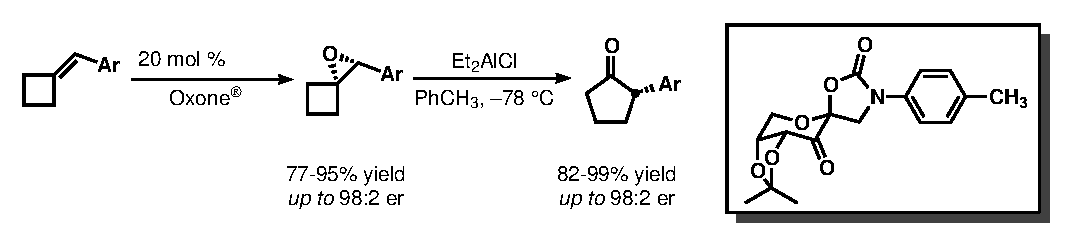
\includegraphics[scale=0.8]{chp_asymmetric/images/shirearrangement}
  \begin{textblock}{1}(16,-1) \cmp{asaaj} \end{textblock}
  \begin{textblock}{1}(4.4,-3.2) \crossrefcmp{asaaj} \end{textblock}
  \caption{Shi's asymmetric epoxidation / rearrangement strategy.}
  \label{sch:asshirearrangement}
\end{Scheme}   
 
  \begin{Scheme}[h]
  \centering
  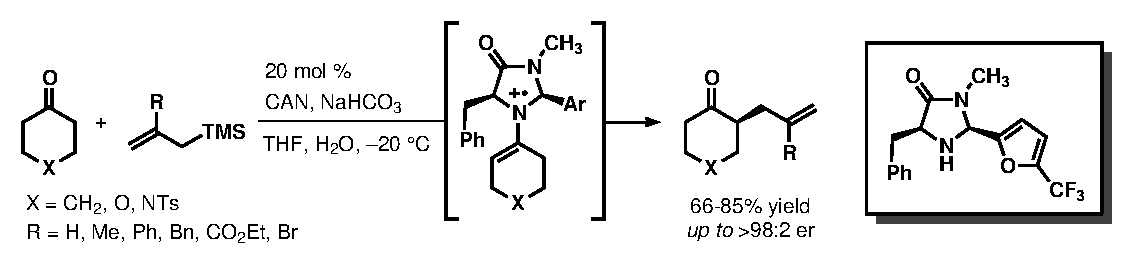
\includegraphics[scale=0.8]{chp_asymmetric/images/macmillansomo}
  \begin{textblock}{1}(9.5,-1) \cmp{asaaja} \end{textblock}
  \begin{textblock}{1}(18.3,-3.2) \cmp{asaajb} \end{textblock}
  \begin{textblock}{1}(6.1,-3.32) \crossrefcmp{asaajb} \end{textblock}
  \caption{Asymmetric allylation with MacMillan's SOMO catalysis.}
  \label{sch:macmillansomo}
\end{Scheme}   
 In 2010 MacMillian reported an intriguing new organocatalytic allylation
 method (\refscheme{macmillansomo}).\footnote{{\frenchspacing Mastracchio, A.; Warkentin, A.
 A.; Walji, A.
 M.; MacMillan, D. W. C. Direct and Enantioselective $\alpha$-Allylation of Ketones \textit{via}
 Singly Occupied Molecular Orbital (SOMO) Catalysis. \textit{Proc. Natl. Acad. Sci. U.S.A.}
 \textbf{2010}, \textit{107}, 20648-20651.} \label{ref:macmillansomo}} Treatment of unfunctionalized
 cycloalkanones with \ref{cmp:asaajb} and CAN facilitates access to a unique three electron
 $\pi$-system (\ref{cmp:asaaja}) through a single electron oxidation event. Face-selective radical
 coupling with substituted allyl trimethylsilanes lead directly to $\alpha$-tertiary substituted
 chiral cycloalkanones with excellent enantioselectivity. 

 
 \subsection{Construction of $\alpha$-Quaternary Centers}
 
 The construction of quaternary centers, especially those possessing all-carbon
 substituents, presents a significant and ongoing challenge for synthetic
 chemists.\footnote{For a reviews on methods for all-carbon quaternary center construction see: (a)
 {\frenchspacing Trost, B. M.; Jiang, C. Catalytic Enantioselective Construction of All-Carbon
 Quaternary Stereocenters. \textit{Synthesis} \textbf{2006}, 369-396.} (b) {\frenchspacing Douglas,
 C.
 J.; Overman, L.
 E.
 Catalytic Asymmetric Synthesis of All-Carbon Quaternary Stereocenters. \textit{Proc. Natl. Acad.
 Sci. U.S.A.} \textbf{2004}, \textit{101}, 5363-5367.}} In their seminal work, Doyle and Jacobsen
 demonstrated a highly enantioselective catalytic asymmetric alkylation of tin enolates to form
 products bearing all-carbon quaternary centers
 (\refscheme{asjacobsentin}).\footnote{{\frenchspacing Doyle, A.
 G.; Jacobsen, E.
 N.
 Enantioselective Alkylations of Tributyltin Enolates Catalyzed by Cr(salen)Cl: Access to Enantiomerically Enriched
 All-Carbon Quaternary Centers. \textit{J. Am. Chem. Soc.} \textbf{2005}, \textit{127}, 62-63.}}
 Tetrasubstituted tin enolates underwent smooth conversion to the $\alpha$-quaternary cycloalkanones
 upon treatment with chromium salen complex \ref{cmp:asaak} and an appropriate alkyl electrophile.
 Cycloalkanones of varying ring sizes were isolated in moderate to high yields with excellent levels of stereocontrol over the newly constructed \ce{C-C} bond. Trisubstituted tin
 enolates that would lead to $\alpha$-tertiary products decomposed under the reaction conditions and
 afforded products in low yields and modest enantioselectivities.
  \begin{Scheme}[h]
  \centering
  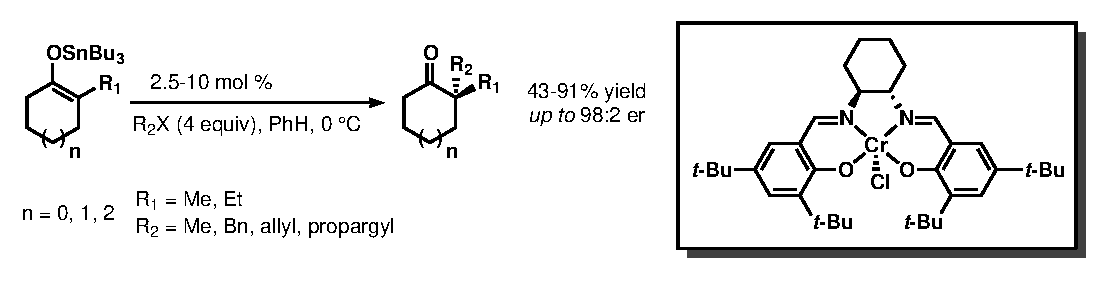
\includegraphics[scale=0.8]{chp_asymmetric/images/jacobsentin}
   \begin{textblock}{1}(12.5,-4) \cmp{asaak} \end{textblock}
  \begin{textblock}{1}(5,-3.35) \crossrefcmp{asaak} \end{textblock}
  \caption{Jacobsen's asymmetric alkylation of tin enolates.}
  \label{sch:asjacobsentin}
\end{Scheme}   
 
The Buchwald\footnote{(a) {\frenchspacing \AA
hman, J.; Wolfe, J.
P.; Troutman, M.
V; Palucki, M.; Buchwald, S. L. Asymmetric Arylation of Ketone Enolates. \textit{J. Am. Chem. Soc.}
 \textbf{1998}, \textit{120}, 1918-1919.} (b) {\frenchspacing Hamada, T.; Chieffi, A.; \AA hman, J.; Buchwald, S. L. An Improved Catalyst for the Asymmetric Arylation of Ketone Enolates. \textit{J. Am. Chem.
 Soc.} \textbf{2002}, \textit{124}, 1261-1268.} \label{ref:asbuchwaldarylation}} and
 Hartwig\footnote{{\frenchspacing Liao, X.; Weng, Z.; Hartwig, J. F. Enantioselective $\alpha$-Arylation of Ketones with Aryl Triflates Catalyzed by Difluorphos Complexes of Palladium
 and Nickel. \textit{J. Am. Chem. Soc.} \textbf{2008}, \textit{130}, 195-200.}} groups introduced similar cross-coupling strategies to access
 all-carbon quaternary centers containing an aromatic substituent. In Buchwald's approach, a two step sequence involving formylation and condensation to prepare an $\alpha$' blocked vinylogous amide
(\ref{cmp:asaal}, \refscheme{asbuchwaldarylation}) was necessary to prevent enolization and coupling
from occuring on the left half of the molecule.
Hartwig focused on indanone and tetralone substrates lacking enolizable $\alpha$' protons
(\refscheme{ashartwigarylation}).
Both methods utilized sodium \textit{tert}-butoxide to generate a sodium enolate that
transmetallated to a chiral Pd(II) or Ni(II) intermediate and ultimately underwent a stereoselective
reductive elimination to forge the new \ce{C-aryl} bond. Buchwald then cleaved the vinylogous amide
protecting group through a dilute acid mediated retro-Claisen condensation. The primary differences
between the two methods were in the choice of chiral ligand and aryl coupling partner. Buchwald
later expanded the substrate scope to include vinyl electrophiles.\footnote{{\frenchspacing Chieffi, A.; Kamikawa, K.; \AA hman, J.; Fox, J. M.; Buchwald, S. L. Catalytic Asymmetric Vinylation of Ketone Enolates. \textit{Org. Lett.}
 \textbf{2001}, \textit{3}, 1897-1900.}}  
   \begin{Scheme}[h]
  \centering
  \includegraphics[scale=0.8]{chp_asymmetric/images/buchwaldarylation}
  \begin{textblock}{1}(2.5,-1.5) \cmp{asaal} \end{textblock}
  \begin{textblock}{1}(17,-0.8) \cmp{asaam} \end{textblock}
  \begin{textblock}{1}(6.1,-3.78) \crossrefcmp{asaam} \end{textblock}
  \caption{Buchwald's asymmetric arylation of $\alpha$'-blocked cycloalkanones.}
  \label{sch:asbuchwaldarylation}
\end{Scheme}   
    \begin{Scheme}[h]
  \centering
  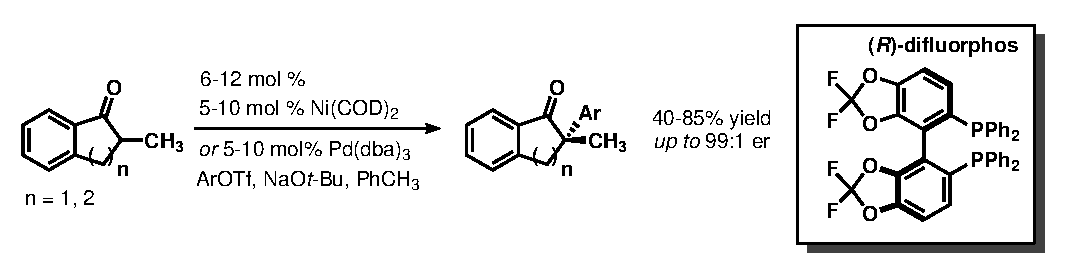
\includegraphics[scale=0.8]{chp_asymmetric/images/hartwigarylation}
  \begin{textblock}{1}(17.5,-0.8) \cmp{asaan} \end{textblock}
  \begin{textblock}{1}(6,-3.35) \crossrefcmp{asaan} \end{textblock}
  \caption{Hartwig's asymmetric arylation of $\alpha$'-blocked cycloalkanones.}
  \label{sch:ashartwigarylation}
\end{Scheme}   
 
 
 The Trost\footnote{{\frenchspacing Trost, B. M.; Schroeder, G. M.
 Palladium-Catalyzed Asymmetric Allylic Alkylation of Ketone Enolates. \textit{J. Am. Chem. Soc.}
 \textbf{2004}, \textit{121}, 6759-6760.}} and Stoltz\footnote{(a) {\frenchspacing Behenna, D.
 C.; Stoltz, B.
 M.
 The Enantioselective Tsuji Allylation. \textit{J. Am. Chem. Soc.} \textbf{2004}, \textit{126}, 15044-15045.} (b)
 {\frenchspacing Mohr, J. T.; Behenna, D. C.; Harned, A. M.; Stoltz, B. M. Deracemization of
 Quaternary Stereocenters by Pd-Catalyzed Enantioconvergent Decarboxylative Allylation of Racemic
 $\beta$-Ketoesters. \textit{Angew. Chem. Int. Ed.} \textbf{2005}, \textit{44}, 6924-6927.}} groups both developed palladium mediated enolate allylation methods that
 generate $\alpha$-keto all-carbon quaternary centers. In Stoltz's work, starting from either the
 $\beta$-keto allyl ester (\ref{cmp:asaao}, \refscheme{stoltzallylation}) or allyl enol carbonate
 (\ref{cmp:asaap}) lead to the same intermediate chiral Pd(II) enolate. Reductive elimination with
 the allyl fragment furnished $\alpha$-quaternary allyl substituted cycloalkanones in high yields
 with excellent levels of enantioselectivity. The mechanistic insight gained through the development of
 this process lead Stoltz to extend this metholodology to allow for the synthesis of
 $\alpha$-tertiary centers through asymmetric protonation as discussed
 previously.\crossref{ref:stoltzprotonation}
  \begin{Scheme}[h]
  \centering
  \includegraphics[scale=0.8]{chp_asymmetric/images/stoltzallylation}
  \begin{textblock}{1}(1.6,-0.9) \cmp{asaao} \end{textblock}
  \begin{textblock}{1}(6.5,-0.9) \cmp{asaap} \end{textblock}
  \caption{Stoltz's asymmetric allylation of Pd-enolates.}
  \label{sch:stoltzallylation}
\end{Scheme}   
 
 With the exception of MacMillan's notable allylation reactions,\crossref{ref:macmillansomo} all of
 the previous examples required a multi-step sequence to install functional group handles that would
 be utilized in the key stereodefining reaction and then ultimately removed to access the target
 cycloalkanone products. We envisioned developing a general strategy to directly access a broad
 range of chiral $\alpha$-substituted cycloalkanones in a single carbon insertion step with aryl--,
 vinyl--, and alkyl-substituted diazoalkanes.
 The versatility and prevalence of the ketone functional group justifies the development of
 methods complementary to those aforementioned.  
 
 \pagebreak
 \section{Discovery of a Catalyst System for Asymmetric $\alpha$-Arylation}
 
 We initially decided to target the enantioselective $\alpha$-arylation of cycloalkanones for two
 primary reasons.
 The Brewer group had recently introduced a mild and operationally simple method for the synthesis of
 aryl-substituted diazoalkanes based on a modified Swern oxidation procedure.\footnote{(a)
 {\frenchspacing Javed, M. I.; Brewer, M. Diazo Preparation \textit{via} Dehydrogenation of
 Hydrazones with Activated DMSO. \textit{Org. Lett.} \textbf{2007}, \textit{9}, 1789-1792.} (b)
 {\frenchspacing Javed, M. I.; Brewer, M. Diphenyldiazomethane. \textit{Org. Synth.} \textbf{2008},
 \textit{85}, 189-195.} \label{ref:asbrewer}}  A simple protocol for preparing the requisite
 diazoalkanes, coupled with the relative stability of aryl-substituted
 diazoalkanes,\footnote{For the relative reactivity of substituted diazoalkanes see \reffigure{nucleophilicity} on page
 \pageref{fig:nucleophilicity}.} made $\alpha$-arylation an ideal proving ground for the first asymmetric insertion
 reactions.

In advance of looking at any catalytic asymmetric reactions, we wanted to run a control experiment
to determine if the products of our reaction would retain their stereochemical information in the
presence of scandium triflate. The Shi group reported earlier that $\alpha$-aryl cyclopentanones
readily racemize on silica gel, presumably through a rather facile enolization
pathway.\crossref{ref:asshitertiary} We began by preparing an optically active sample of
(\textit{R})-2-phenylcycloheptanone according to a three step sequence using the asymmetric
protonation chemistry developed by Yanagisawa
(\refscheme{asracemizationone}).\crossref{ref:asyanagisawa}
  \begin{Scheme}[h]
  \centering
  \includegraphics[scale=0.8]{chp_asymmetric/images/racemizationone}
  \begin{textblock}{1}(0.35,-0.7) \cmp{ascyclohexanone} \end{textblock}
  \begin{textblock}{1}(3.3,-3.3) \cmp{diazoaa} \end{textblock}
  \begin{textblock}{1}(5.8,-0.7) \cmp{xaaa} \end{textblock}
  \begin{textblock}{1}(11.6,-0.7) \cmp{asaaq} \end{textblock}
  \begin{textblock}{1}(18,-0.7) \cmp{asaar} \end{textblock}
  \caption{Preparation of optically active 2-phenylcycloheptanone.}
  \label{sch:asracemizationone}
\end{Scheme}   
Scandium-catalyzed homologation of cyclohexanone with phenyldiazomethane (\ref{cmp:diazoaa})
afforded racemic 2-phenylcycloheptanone (\ref{cmp:xaaa}) in a 65\% distilled yield. Dropwise
addition of 0.95 equivalents of LDA to \ref{cmp:xaaa} followed by trapping with TMSCl selectively
delivered the thermodynamic enol silane \ref{cmp:asaaq} in 85\% yield.
Asymmetric protonation according to the reported conditions provided access
(\textit{R})-2-phenylcycloheptanone (\ref{cmp:asaar}) in 83\% yield and 95:5 er in our
hands.\footnote{The Yanagisawa group reported a 95\% yield and 98.5:1.5 er for the preparation of 
\ref{cmp:asaar}.
See reference \ref{ref:asyanagisawa} for details.} Exposure of \ref{cmp:asaar} to phenyldiazomethane,
\ce{Sc(OTf)3}, or the combination of the two (toluene, 0 \degc, 6 h) resulted in no loss of enantiopurity (95:5 er by chiral SFC analysis). This promising initial result indicated that chiral homologation products should be configurationally
stable under conditions of scandium catalysis. \refscheme{asracemizationone} also
underscores the benefits of eliminating the three step sequence that must precede asymmetric protonation, as products like \ref{cmp:asaar} could
be accessible in a single asymmetric homologation step.


We also wanted to run a simple mechanistic control to determine if the scandium-catalyzed reactions
proceeded through a pathway involving an epoxide intermediate. House had previously shown that
epoxides formed in Lewis acid mediated ring expansion reactions readily underwent rearrangement
to the corresponding aldehydes.\footnote{{\frenchspacing House, H. O.; Grubbs, E. J.; Gannon, W. F.
The Reaction of Ketones with Diazomethane. \textit{J. Am. Chem. Soc.} \textbf{1960}, \textit{82},
4099-4106.}} We had never detected any epoxide or aldehyde byproducts in any scandium catalyzed ring expansion reactions (by $^1$H NMR), but regardless, we carried out the experiment shown in \refscheme{asepoxideexperiment}. Epoxide \ref{cmp:asaara} was obtained
through standard chemistry in an 87\% yield over two steps from cyclohexanone. Subjecting
epoxide \ref{cmp:asaara} to 10 mol \% \ce{Sc(OTf)3} at $-78$ \degc\  for 5 days resulted in $<$2\%
conversion, clearly indicating that it was improbable the scandium catalyzed homologation reactions
involved an epoxide intermediate. The most plausible mechanism was that
previously discussed in the literature, a concerted collapse of a diazonium
betaine to directly deliver the observed ring expanded products
(\refscheme{mechanism}, page \pageref{sch:mechanism}).\crossref{ref:asgutscherev}

 \begin{Scheme}[h]
  \centering
  \includegraphics[scale=0.8]{chp_asymmetric/images/epoxideexperiment}
  \begin{textblock}{1}(3.4,-0.2) \crossrefcmp{ascyclohexanone} \end{textblock}
   \begin{textblock}{1}(9.4,-0.2) \cmp{asaara} \end{textblock}
   \begin{textblock}{1}(14.8,-0.2) \crossrefcmp{xaaa} \end{textblock}
%   \begin{textblock}{1}(11.6,-0.7) \cmp{asaaq} \end{textblock}
%   \begin{textblock}{1}(18,-0.7) \cmp{asaar} \end{textblock}
  \caption{Mechanistic probe of plausible epoxide rearrangement pathway.}
  \label{sch:asepoxideexperiment}
\end{Scheme}   

\subsection{Optimized Conditions for Consistent Reactivity}

\begin{wrapfigure}{r}{2.8in}
  \centering
  \vspace{-40pt}
  \includegraphics[scale=0.3]{chp_asymmetric/images/scandiumhydratedortep}
  %\begin{textblock}{5}(-1,-4) \small \textsf{test}\end{textblock}
  \caption{Crystal structure of \ce{Sc(H2O)9(OTf)3}.}
  \vspace{-25pt}
  \label{fig:asscandiumhydrated}
  \end{wrapfigure}
The newly discovered scandium catalyzed homologation reactions often gave variable and
unpredictable results that appeared to depend on the source of \ce{Sc(OTf)3} and batch of
diazoalkane solution.
In order to obtain meaningful results when optimizing conditions for asymmetric reactions, the reaction
variability would first need to be understood and mitigated. At the time this project began,
no special protocols were in place to purify any of the reaction components. The \ce{Sc(OTf)3} was
often used as received and the aryl-diazoalkanes were prepared by directly following the
reported Brewer procedure.\crossref{ref:asbrewer} In order to mimimize reaction variability, efforts
were undertaken to rigorously purify and dry \textit{all} reaction components: solvents,
\ce{Sc(OTf)3}, ketones, diazoalkanes, and ligands.

Scandium triflate is a deliquescent solid that rapidly absorbs significant quantities of atmospheric
moisture. Crystallographic data from the literature has shown \ce{Sc(OTf)3} to bind up to nine water
molecules (\reffigure{asscandiumhydrated}).\footnote{{\frenchspacing Abbasi, A.; Lindqvist-Reis, P.;
Eriksson, L.; Sandstr\"{o}m, D.; Lidin, S.; Persson, I.; Sandstr\"{o}m, M. Highly Hydrated Cations:
Deficiency, Mobility, and Coordination of Water in Crystalline Nonahydrated Scandium(III),
Yttrium(III), and Lanthanoid(III) Trifluoromethanesulfonates. \textit{Chem. Eur. J.} \textbf{2005},
\textit{11}, 4065-4077.}} Although \ce{Sc(OTf)3} is known to retain catalytic activity even in
aqueous media,\footnote{{\frenchspacing Kobayashi, S.; Hachiya, I. Lanthanide Triflates as
Water-Tolerant Lewis Acids. Activation of Commercial Formaldehyde Solution and Use in the Aldol
Reaction of Silyl Enol Ethers with Aldehydes in Aqueous Media. \textit{J. Org. Chem.} \textbf{1994},
\textit{59}, 3590-3596.}} we had anecdotal evidence that suggested drier conditions lead to higher
reaction efficiencies for diazoalkane insertion reactions.\footnote{Reaction rates can be
approximated visually by the evolution of nitrogen gas and the loss of the characteristic
diazoalkane color.} When Kobayashi first introduced \ce{Sc(OTf)3} in
1993, he reported drying the salt at 200 \degc\ under high vacuum before use.\footnote{{\frenchspacing Kobayashi, S.; Hachiya, I.; Araki, M.; Ishitani, H.
Scandium Trifluoromethanesulfonate (\ce{Sc(OTf)3}). A Novel Reusable Catalyst in the Diels-Alder
Reaction. \textit{Tetrahedron Lett.} \textbf{1993}, \textit{34}, 3755-3758.}} We took this drying
method one step further and dried commercial \ce{Sc(OTf)3} under high vacuum at 200 \degc\  with
inline \ce{P2O5} for 24 hours before taking the salt into an inert atmosphere glove box using
rigorous Schlenk techniques.

Diazoalkane solutions were originally prepared according to the general procedure reported by Brewer.\crossref{ref:asbrewer} In a typical experimental procedure, a
solution of the hydrazone and triethylamine were added dropwise to a cold solution of chlorodimethylsulfonium chloride, formed \textit{in situ} from oxalyl chloride and DMSO (\refscheme{asbrewerswern}).
After stirring for an hour at $-$78 \degc, the reaction mixture was filtered to remove insoluble
triethylammonium chloride and carefully concentrated to remove THF. The neat diazoalkane was then
dissolved in toluene and stored at $-78$ \degc. Following this procedure gave fairly pure
diazoalkane solutions, but we wanted to be sure to remove all traces of Lewis basic impurities. We modified the procedure to include an aqueous workup which
removed any residual triethylamine and DMSO. The oxidation was run for one hour
in a 9:1 \ce{Et2O}:\ce{CH2Cl2} solvent mixture and immediately poured into a separatory funnel
containing an ice cold 50\% solution of aqueous \ce{NH4Cl}. The \ce{NH4Cl} layer was drained and the
organics were washed with \ce{H2O} and saturated \ce{NaHCO3} before drying over solid \ce{K2CO3}. Filtration,
concentration, and finally dissolution in toluene afforded exceptionally pure diazoalkane solutions. 
\begin{Scheme}[h]
  \centering
  \includegraphics[scale=0.8]{chp_asymmetric/images/brewerswern}
  \begin{textblock}{1}(16,-0.7) \crossrefcmp{diazoaa} \end{textblock}
  \caption{Original preparation of aryl-substituted diazoalkanes by Brewer.}
  \label{sch:asbrewerswern}
\end{Scheme}  

Unfortunately, by performing an aqueous workup on the diazoalkanes, we inadvertently introduced an
additional problem. Occasionally we would observe the formation of a white precipitate in some of
the diazoalkane solutions after prolonged storage at $-78$ \degc. After numerous unsuccessful
attempts to isolate and characterize the white precipitate, we realized that it was residual water
from inefficient drying of diazoalkane solution after workup. Although \ce{K2CO3} was not the most
efficient dessicant, the highest yields of diazoalkane were obtained with solutions dried over
\ce{K2CO3}. The residual water was ultimately best removed by carefully gravity filtering the
diazoalkane solution at $-$78 \degc\ in a cold-jacketed dropping funnel, then storing the clear
solution over 3\AA\ molecular sieves.

With rigorously dried \ce{Sc(OTf)3}, pure and dry diazoalkane solutions, distilled ketones, and
solvents passed through an alumina column and stored over 3\AA\ molecular
sieves,\footnote{{\frenchspacing Williams, D.
B.
G.; Lawton, M.
Drying of Organic Solvents: Quantitative Evaluation of the Efficiency of Several Desiccants.
\textit{J. Org. Chem.} \textbf{2010}, \textit{75}, 8351-8354.}} dramatic increases in reaction
efficiency were observed.\footnote{{\frenchspacing Rendina, V. L.; Kaplan, H. Z.; Kingsbury, J. S.
Highly Efficient and Enantioselective $\alpha$-Arylation of Cycloalkanones by Scandium-Catalyzed
Diazoalkane-Carbonyl Homologation. \textit{Synthesis} \textbf{2012}, \textit{44}, 686-693.}
\label{ref:asrendinapsp}} More importantly though, reactions worked in a predictable and
reproducible manner.
When we had prepared racemic 2-phenylcycloheptanone (\ref{cmp:xaaa}) previously,
the reaction was run with 10 mol \% \ce{Sc(OTf)3} and 1.1 equivalents of phenyldiazomethane
(\ref{cmp:diazoaa}) for 16 hours (\refscheme{asracemizationone},
page \pageref{sch:asracemizationone}).
After workup and attempted purification by silica gel chromatography, the desired product was obtained in a quantitative yield but was contaminated with overhomologation byproducts.\footnote{Not isolated, but double insertion was detected by low resolution mass spectrometry. \ce{C20H23O} [M+H]$^+$: 279.1749.} Careful K\"{u}gelrohr distillation delivered analytically pure material in a modest 65\% yield. Under the new drier conditions, running the reaction for 15 minutes with 0.5 mol \% \ce{Sc(OTf)3}, 1.0
equivalents of phenyldiazomethane, and 1.2 equivalents of cyclohexanone, a 92\% isolated yield was
obtained after silica gel chromatography. By modifying the stoichiometry, no further purification
away from overhomologation byproducts was necessary. The reaction rates were so high, an 18 gauge
exit needle was needed to relieve excess pressure generated by the copious amounts of nitrogen gas evolved.
\begin{Scheme}[h]
  \centering
  \includegraphics[scale=0.8]{chp_asymmetric/images/rendinapspsubstrates}
  \begin{textblock}{1}(13.5,-10.3) \cmp{xaac} \end{textblock}
  \begin{textblock}{1}(6.5,-10.2) \crossrefcmp{diazoaa} \end{textblock}
  %row 1
  \begin{textblock}{1}(2,-6.6) \cmp{xaab} \end{textblock}
  \begin{textblock}{1}(5.5,-6.6) \cmp{xaad} \end{textblock}
  \begin{textblock}{1}(9,-6.6) \cmp{xaae} \end{textblock}
  \begin{textblock}{1}(12.8,-6.6) \cmp{xaaf} \end{textblock}
  \begin{textblock}{1}(16.5,-6.6) \cmp{xaag} \end{textblock}
  % row 2
\begin{textblock}{1}(2,-1.5) \cmp{xaah} \end{textblock}
\begin{textblock}{1}(5.5,-1.5) \cmp{xaai} \end{textblock}
\begin{textblock}{1}(9,-1.5) \crossrefcmp{xaaa} \end{textblock}
\begin{textblock}{1}(12.8,-1.5) \cmp{xaaj} \end{textblock}
\begin{textblock}{1}(18.2,-3.3) \cmp{xaak} \end{textblock}
  \caption{Highly efficient insertion reactions with aryl-diazoalkanes.}
  \label{sch:asrendinapspsubstrates}
\end{Scheme}  

The newly optimized conditions were successfully applied to a number of ring expansion reactions
with aryl-substituted diazoalkanes (\refscheme{asrendinapspsubstrates}).\crossref{ref:asrendinapsp}
Good scope with regard to the diazoalkane and ketone ring size were demonstrated. Reactions
catalyzed by low loadings of \ce{Sc(OTf)3} (0.5--7 mol \%) were complete in $<$1 hour and gave high
yields in all cases tested. In addition to being reliable and efficient, the reactions could be
scaled to afford gram quantities of homologation products (\ce{->}\ref{cmp:xaac}). With reliable
protocols in place and an understanding that water was the culprit of previous reproducibility
issues, we were prepared to examine asymmetric insertion reactions. 

\subsection{Early Results with Bis(oxazoline) Ligands}

We began by evaluating the PyBOX\crossref{ref:asevans} and bipyridine
diol\crossref{ref:askobayashistructure} ligand frameworks previously reported to form competent
chiral scandium complexes (\refscheme{asinitialligandscreen}). In an inert atmosphere glove box,
\ce{Sc(OTf)3} was stirred in toluene with a slight excess of the ligand for 1.5 hours to pre-form
the ligand-metal complex. During complexation, 25 mol \% THF was added as a cosolvent to help
solubilize the scandium salt. The catalyst mixture was removed from the glove box, connected to a nitrogen manifold, and stirred with cyclohexanone for 15 minutes. After cooling to $-$78 \degc,
phenyldiazomethane (\ref{cmp:diazoaa}) was added in a single portion and the reactions were stirred
until no further evolution of nitrogen gas was observed. An aliquot of the reaction mixture was purified by
preparative thin-layer chromatography and analyzed for optical purity by chiral SFC analysis in
comparison with authentic racemic material. Commercially available PyBOX ligand \ref{cmp:asaas}
delivered \ref{cmp:xaan} in a measurable 56:44 er. The bipyridine diol ligand \ref{cmp:asaat} afforded racemic product. We also tested a
commercially available Salen\footnote{{\frenchspacing Larrow, J. F.; Jacobsen, E. N. Asymmetric
Processes Catalyzed by Chiral (Salen)Metal Complexes. \textit{Topics Organomet. Chem.} \textbf{2004}, \textit{6},
123-152.}} ligand which produced nearly racemic product. Ligands \ref{cmp:asaat} and \ref{cmp:asaau}
were likely not stable under the reaction conditions, as diazoalkanes are known to undergo \ce{O-H}
insertion reactions.\footnote{See the discussion in Chapter \ref{chp:diazobkg} for examples.}
Etherification of the two \ce{O-H} groups would decrease the binding affinity of the ligand and
metal, leading to background reaction by uncomplexed scandium.
\begin{Scheme}[h]
  \centering
  \begin{textblock}{1}(3.1,2.2) \crossrefcmp{ascyclohexanone} \end{textblock}
  \begin{textblock}{1}(6.2,2.2) \crossrefcmp{diazoaa} \end{textblock}
  \begin{textblock}{1}(13.3,2.6) \cmp{xaan} \end{textblock}
  \begin{textblock}{1}(2.6,5.3) \cmp{asaas} \end{textblock}
  \begin{textblock}{1}(8.2,5.3) \cmp{asaat} \end{textblock}
  \begin{textblock}{1}(17,3.2) \cmp{asaau} \end{textblock}
  \includegraphics[scale=0.8]{chp_asymmetric/images/initialligandscreen}
  \caption{Initial ligand screening.}
  \label{sch:asinitialligandscreen}
\end{Scheme}  



Previous experiments had shown that Lewis basic impurities could dramatically affect reaction
efficiency. Reactions run with PyBOX ligand \ref{cmp:asaas} visually progressed more slowly than
those without the ligand present. We believed that by excising the bridging pyridine ring, we
could decrease the Lewis basicity of the ligand while simultaneously bringing the ligand blocking
groups closer to the metal center. The well known bis(oxazoline) ligand class retains the blocking
group structure of the PyBOX ligands, but contains a methylene bridge between the two oxazoline
units. While scandium PyBOX crystal structures have been reported, there are no examples of scandium
bis(oxazoline) structures. In contrast, a preponderance of bis(oxazoline) copper
complexes have been reported.\footnote{Nineteen Cu(II) bis(oxazoline) crystal
structures were discussed by Desimoni in a 2006 review. {\frenchspacing Desimoni, G.; Faita, G.;
J\o rgensen, K.
A.
C$_2$-Symmetric Chiral Bis(oxazoline) Ligands in Asymmetric Catalysis. \textit{Chem. Rev.}
\textbf{2006}, \textit{106}, 3561-3651.} \label{ref:asboxreview}} \reffigure{ascoppercomplexes}
shows a direct comparison between copper PyBOX\footnote{{\frenchspacing Evans, D. A.; Kozlowski, M. C.; Murry, J. A.; Burgey,
C. S.; Campos, K. R.; Connell, B. T.; Staples, R. J. C$_2$-Symmetric Copper (II) Complexes as Chiral
Lewis Acids. Scope and Mechanism of Catalytic Enantioselective Aldol Additions of Enolsilanes to
(Benzyloxy)acetaldehyde. \textit{J. Am. Chem. Soc.} \textbf{1999}, \textit{121}, 669-685.}} and
copper BOX\footnote{{\frenchspacing Evans, D. A.; Johnson, J. S.; Burgey, C. S.; Campos,
K. R. Reversal in Enantioselectivity of \textit{tert}-Butyl Versus Phenyl-Substituted Bis(oxazoline)
Copper(II) Catalyzed Hetero Diels-Alder and Ene Reactions. Crystallographic and Mechanistic Studies.
\textit{Tetrahedron Lett.} \textbf{1999}, \textit{40}, 2879-2882.}} hexafluoroantimonate salts
containing the same valine-derived oxazoline units. The BOX complex (right,
\ref{cmp:asaaw}) shows a smaller through space N$_{ox}$\ce{-}N$_{ox}$ distance (1.13 \AA\  shorter)
and a significantly compressed N$_{ox}$\ce{-}Cu\ce{-}N$_{ox}$ internal angle relative to the
corresponding PyBOX complex (left, \ref{cmp:asaav}).
\begin{figure}[t]
\vspace{1.65in}
  \centering
     \begin{textblock}{1}(0.7,1.2) \cmp{asaav} \end{textblock}
   \begin{textblock}{1}(11.7,1.2) \cmp{asaaw} \end{textblock}
  \includegraphics[scale=0.8]{chp_asymmetric/images/evanscopper}
  \begin{textblock}{5}(2,0.5) \small \textsf{N$_{ox}$\ce{-}N$_{ox}$ distance 3.95
  \AA \\ $\angle$ N$_{ox}$\ce{-}Cu\ce{-}N$_{ox}$ 158.4$^\circ$}\end{textblock}
  \begin{textblock}{5}(12.5,0.5) \small \textsf{N$_{ox}$\ce{-}N$_{ox}$ distance 2.82
  \AA \\ $\angle$ N$_{ox}$\ce{-}Cu\ce{-}N$_{ox}$ 91.6$^\circ$}\end{textblock} 
  \begin{textblock}{1}(-1.5,-9)
  \includegraphics[scale=0.3]{chp_asymmetric/images/copperpyboxortep}\end{textblock}
  \begin{textblock}{1}(10,-9)
  \includegraphics[scale=0.3]{chp_asymmetric/images/copperboxortep}\end{textblock}
  \vspace{0.6in}
  \caption{Comparison of copper PyBOX and BOX complexes. Counterions omitted for clarity.}
  \label{fig:ascoppercomplexes}
\end{figure}  


We quickly tested several readily available BOX ligands, hoping the different steric
and electronic properties would translate into increased levels of stereoinduction
(\refscheme{asfirstboxscreen}).
We were pleased to see that ligand \ref{cmp:boxasab} provided much higher levels of selectivity. Different blocking
groups (\ref{cmp:boxasaa}, \ref{cmp:boxasac}) and bis(oxazoline) \ref{cmp:boxasad} resulted in
lower selectivity. Excited by this promising lead, we initiated a broader screen of BOX ligands
(\refscheme{asbigboxscreen}). The bis(oxazoline) framework contains three diversity sites for
C$_2$-symmetric ligands, making it a highly tunable and privileged ligand
class.\crossref{ref:asboxreview} We wanted to simultaneously optimize with regard to both backbone substitution and the amino alcohol derived blocking groups.\footnote{For a lead reference on the
benefits of multi-factor optimization see: {\frenchspacing Lendrem, D.; Owen, M.; Godbert,
S. DOE (Design of Experiments) in Development Chemistry: Potential Obstacles. \textit{Org. Process
Res. Dev.} \textbf{2001}, \textit{5}, 324-327.}}
 \begin{Scheme}[t]
  \centering
   \begin{textblock}{1}(3.1,2.3) \crossrefcmp{ascyclohexanone} \end{textblock}
   \begin{textblock}{1}(6.2,2.3) \crossrefcmp{diazoaa} \end{textblock}
   \begin{textblock}{1}(14,2) \crossrefcmp{xaan} \end{textblock}
   \begin{textblock}{1}(1.6,5.3) \cmp{boxasaa} \end{textblock}
    \begin{textblock}{1}(6.4,5.3) \cmp{boxasab} \end{textblock}
     \begin{textblock}{1}(12,5.3) \cmp{boxasac} \end{textblock}
      \begin{textblock}{1}(17,5.3) \cmp{boxasad} \end{textblock}
  \includegraphics[scale=0.8]{chp_asymmetric/images/firstboxscreen}
  \caption{Screen of commercially available bis(oxazoline) ligands.}
  \label{sch:asfirstboxscreen}
\end{Scheme}

Examination of the results in \refscheme{asbigboxscreen} showed that backbone substitution was
integral to obtaining high levels of induction. Ligands lacking geminal substitution on the bridging
methylene are known to tautomerize, which could adversely impact the ligand-metal
binding. We prepared a series of ligands containing cyclic backbone
substitution to probe the effect of bite angle on enantioselectivity. Davies and coworkers had
prepared a similar series of BOX ligands and observed a strong dependence of enantioselectivity on ligand bite
angle in copper catalyzed Diels-Alder reactions.\footnote{(a) {\frenchspacing Davies, I. W. I. W.;
Gerena, L.; Castonguay, L.; Senanayake, C.
H.; Larsen, R. D.; Verhoevena, T. R.; Reidera, P. J.; Verhoeven, T. R.; Reider, P. J. The Influence
of Ligand Bite Angle on the Enantioselectivity of Copper(II)-Catalysed Diels-Alder Reactions.
\textit{Chem. Commun.} \textbf{1996}, 1753-1754.} (b) {\frenchspacing Davies, I. W.; Deeth, R. J.;
Larsen, R. D.; Reider, P. J. A CLFSE/MM Study on the Role of Ligand Bite-Angle in Cu(II)-Catalyzed
Diels-Alder Reactions. \textit{Tetrahedron Lett.} \textbf{1999}, \textit{40}, 1233-1236.}\label{ref:asdaviesdielsalder}} \begin{Scheme}[p]
  \centering
%% header row
  \begin{textblock}{1}(3,2.3) \crossrefcmp{ascyclohexanone} \end{textblock}
  \begin{textblock}{1}(6.2,2.3) \crossrefcmp{diazoaa} \end{textblock}
  \begin{textblock}{1}(13.3,2.6) \crossrefcmp{xaan} \end{textblock}
%% row 1
   \begin{textblock}{1}(7.4,5.9) \crossrefcmp{boxasaa} \end{textblock}
    \begin{textblock}{1}(11.8,5.9) \crossrefcmp{boxasab} \end{textblock}
     \begin{textblock}{1}(16.5,5.9) \crossrefcmp{boxasac} \end{textblock}
 %% row 2
   \begin{textblock}{1}(2,11) \cmp{ligandac} \end{textblock}
    \begin{textblock}{1}(7.2,11) \cmp{ligandad} \end{textblock}
     \begin{textblock}{1}(12,11) \cmp{ligandae} \end{textblock}
     \begin{textblock}{1}(16.8,11) \cmp{ligandaf} \end{textblock}
 %% row 3
    \begin{textblock}{1}(1.8,15.8) \cmp{boxasae} \end{textblock}
    \begin{textblock}{1}(7,15.8) \cmp{boxasaf} \end{textblock}
     \begin{textblock}{1}(12,15.8) \cmp{ligandal} \end{textblock}
     \begin{textblock}{1}(16.8,15.8) \cmp{boxasag} \end{textblock}
%% row 4
    \begin{textblock}{1}(4.2,20) \cmp{boxasah} \end{textblock}
    \begin{textblock}{1}(9.35,20) \cmp{boxasai} \end{textblock} %% dibenzyl gemdimethyl
     \begin{textblock}{1}(14.65,20) \cmp{ligandaa} \end{textblock} %% indabox
  \includegraphics[scale=0.8]{chp_asymmetric/images/bigboxscreen}
  \vspace{10pt}
  \caption{Wider screen of bis(oxazoline) ligands reveals two optimum ligands.}
  \label{sch:asbigboxscreen}
\end{Scheme}
Ligand \ref{cmp:ligandac}, containing a three-membered ring backbone, showed the highest selectivity
(87:13 er) among the series, consistent with the results obtained by Davies. However, no clear trend
emerged from these data. Ligand \ref{cmp:ligandad} showed a significant drop in selectivty (55:45
er), which was regained again with ligand \ref{cmp:ligandae} (85.5:14.5 er). Purity of the ligand
may have been a determining factor, as ligand \ref{cmp:ligandad} was not as easy to crystallize
cleanly as the others in the series. Some of the ligands in \refscheme{asbigboxscreen} have also
been observed to crystallize as a solvate complex with water. Changing the blocking group to a single phenyl ring on each half and placing geminal methyl groups
on the backbone afforded comparable levels of selectivity (ligand \ref{cmp:boxasae}, 85:15 er).
Installing geminal ethyl groups on the backbone increased the selectivity slightly
(\ref{cmp:boxasaf}, 89:11 er), but with geminal benzyl groups the selectivity dropped
(\ref{cmp:ligandal}, 57:43 er). Running with \textit{tert}-leucine derived BOX \ref{cmp:boxasag}
gave completely racemic material. Curiously, phenylalanine derived BOX \ref{cmp:boxasai} and
indanyl BOX \ref{cmp:ligandaa} gave an identical 91:9 er. Material from the reaction with ligand
\ref{cmp:boxasai} was isolated in an excellent 93\% yield.

We hoped at this point that we could spend time further refining and optimizing the reaction
conditions with commercially available BOX ligand \ref{cmp:boxasai} to improve the selectivity beyond 91:9 er.
Significant effort was invested in optimizing the reaction with regard to stoichiometry, solvent, temperature, and even
various additives (\reftable{asoptimization}). Reactions run in \ce{CH2Cl2} afforded lower
selectivities, but the values were consistent regardless of changes with respect to
stoichiometry (entries 1--6). Using coordinating solvents either shut down the reaction in the case of \ce{CH3CN} (entry
7), or gave lower levels of selectivity in the case of \ce{Et2O} (entry 8). Entry 10, run in
toluene at $-$90 \degc, showed the highest selectivity at 92.5:7.5 er. The freezing point of toluene
($-$95 \degc) and the practicality of running reactions at temperatures lower than $-78$ \degc\
prevented us from looking at even lower temperatures. We looked at various additives other than THF
hoping that the appropriate additive could help solubilize or stabilize the chiral catalyst. Adding
25 mol \%  \ce{CH3CN}, \ce{Et2O}, or DME  effectively had no impact on the
selectivity (entries 11--13). Addition of 2,6-lutidine or pyridine had a detrimental effect on both
reaction kinetics and the observed enantioselectivity (entries 14, 15). This may help rationalize
why reactions with PyBOX ligand \ref{cmp:asaas} were sluggish and only moderately selective. We also
found that although THF appeared to help solubilize the catalyst mixture, it was unnecessary to
obtain high levels of selectivity (entry 17). By pre-mixing the catalyst suspension with
cyclohexanone for 15 minutes, the reaction mixture became homogeneous and afforded comparable
levels of enantioselectivity (90:10 er).
Dropping the catalyst loading to 5 mol \% had no effect on the enantioselectivity and increasing the catalyst loading to 20 mol \% gave an identical result (entries 18, 19).

\singlespacing
\ctable[
	caption = Attempts to optimize reaction conditions with bis(oxazoline) ligand \ref{cmp:boxasai}.,
	label = nowidth,
	pos = t,
	label = tbl:asoptimization,
	doinside = \footnotesize,
	botcap,
	notespar
]{ccccccccc}{
	\tnote{\textit{Conditions:} 0.1 M in solvent with 25 mol \% additive, 1.0 equiv
	phenyldiazomethane (\ref{cmp:diazoaa}). Ligand \ref{cmp:boxasai} and \ce{Sc(OTf)3} pre-complexed
	for 1.5 hrs at 23 \degc. Stirred 15 min with cyclohexanone (\ref{cmp:ascyclohexanone}) before cooling.}
	\tnote[b]{Determined by chiral SFC analysis in comparison with authentic racemic material.}
	\tnote[c]{Isolated yield after silica gel chromatography.}
	\tnote[d]{Run with 18 mg of powdered sieves and 25 mol \% THF.}
	\begin{textblock}{1}(3.1,-14) \crossrefcmp{ascyclohexanone} \end{textblock}
	\begin{textblock}{1}(6,-14) \crossrefcmp{diazoaa} \end{textblock}
	\begin{textblock}{1}(10.1,-15.95) \crossrefcmp{boxasai} \end{textblock}
	\begin{textblock}{1}(14.4,-14.2) \crossrefcmp{xaan} \end{textblock}
}{
\multicolumn{9}{c}{
\includegraphics[scale=0.8]{chp_asymmetric/images/conditionscreenhead} \vspace{10pt}
} \\
\FL
%%% begin header line
\multirow{2}{*}{entry\tmark} &  mol \% & mol \% & equiv & \multirow{2}{*}{solvent} & \multirow{2}{*}{additive} & \multirow{2}{*}{temp (\degc)} & \multirow{2}{*}{er (\textit{R}/\textit{S})\tmark[b]} & \multirow{2}{*}{yield (\%)\tmark[c]} \NN
&\ce{Sc(OTf)3} & \ref{cmp:boxasai} & \ref{cmp:ascyclohexanone} & & & & & \ML 
%% end header line, begin data
1 & 10 & 11 & 1.1 & CH$_2$Cl$_2$ & THF & $-$78   & 84.5:15.5 (\textit{S}) & 99 \\
2\tmark[d] & 10 & 11 & 1.2 & CH$_2$Cl$_2$ & 3\AA\ sieves & $-$78   & 84:16 (\textit{S}) & 99 \\
3\tmark[d] & 10 & 11 & 1.2 & CH$_2$Cl$_2$ & 4\AA\ sieves & $-$78   & 84.5:15.5 (\textit{S}) & $>$98 \\
4 & 10 & 11 & 1.5 & CH$_2$Cl$_2$ & THF & $-$78   & 83.5:16.5 (\textit{S}) & $>$98 \\
5 & 10 & 11 & 2.0 & CH$_2$Cl$_2$ & THF & $-$78   & 83.5:16.5 (\textit{S}) & 98 \\
6 & 10 & 11 & 4.0 & CH$_2$Cl$_2$ & THF & $-$78   & 83:17 (\textit{S}) & 95 \\
7 & 10 & 11 & 1.2 & \ce{CH3CN} & $-$ & $-$78   & nd & nr \\
8 & 10 & 11 & 1.2 & Et$_2$O & $-$ & $-$78   & 75:25 (\textit{S}) & nd \\
9 & 10 & 11 & 1.2 & toluene & THF & $-$78   & 91:9 (\textit{S}) & 93 \\
\rowcolor{gray!15} 10 & 10 & 11 & 1.2 & toluene & THF & $-$90   & \textbf{92.5:7.5 (\textit{S})} &
nd \\
11 & 10 & 11 & 1.2 & toluene & CH$_3$CN & $-$78   & 90.5:9.5 (\textit{S}) & nd \\
12 & 10 & 11 & 1.2 & toluene & Et$_2$O & $-$78   & 90.5:9.5 (\textit{S}) & nd \\
13 & 10 & 11 & 1.2 & toluene & DME & $-$78   & 91:9 (\textit{S}) & nd \\
14 & 10 & 11 & 1.2 & toluene & 2,6-lutidine & $-$78   & 72.5:27.5 (\textit{S}) & nd \\
15 & 10 & 11 & 1.2 & toluene & pyridine & $-$78   & 57.5:42.5 (\textit{S}) & nd \\
16 & 10 & 11 & 1.2 & toluene & NaOTf & $-$78   & 90.5:9.5 (\textit{S}) & nd \\
17 & 10 & 11 & 1.2 & toluene & $-$ & $-$78   & 90:10 (\textit{S}) & nd \\
18 & 5 & 5.5 & 1.2 & toluene & THF & $-$78   & 90.5:9.5 (\textit{S}) & nd \\
19 & 20 & 22 & 1.2 & toluene & THF & $-$78   & 90.5:9.5 (\textit{S}) & nd \LL}
\doublespacing

\subsection{Optimal Conditions for Medium Ring Arylation}
  
After struggling to obtain higher selectivities through extensive optimization, we wanted to
glean more information about the catalyst-ligand complex. $^1$H NMR analysis of scandium BOX
mixtures showed significant line broadening and multiple additional signals, consistent with a
poorly defined and fluxional catalyst structure. By constrast, $^1$H NMR analysis of scandium PyBOX
mixtures showed cleanly resolved signals slightly offset from the uncomplexed ligand, consistent with a well
defined monomeric catalyst species in solution. Attempts to obtain a solid state structure of
scandium BOX complexes lead to a number of bis(oxazoline) triflate salt structures
(\ce{->}\ref{cmp:xabf}, \refscheme{boxtriflatesalt}). 
 \begin{Scheme}[h]
 % \centering
  \begin{textblock}{1}(9,1) \includegraphics[scale=0.8]{chp_asymmetric/images/triflatesaltformation}
  \end{textblock}
   \begin{textblock}{1}(10.2,6.5) \crossrefcmp{ligandal} \end{textblock}
   \begin{textblock}{1}(16.6,6.5) \cmp{xabf} \end{textblock}
  \includegraphics[scale=0.35]{chp_asymmetric/images/xray/xabf_nolabels}
  \caption{Formation of a triflate salt with attempts to crystallize scandium bis(oxazoline) complexes.}
  \label{sch:boxtriflatesalt}
\end{Scheme}
It is plausible that residual water on the
\ce{Sc(OTf)3}, ligand, or in the solvents, caused water to exchange for one of the triflate ligands,
producing a Br{\o}nsted acid.\footnote{{\frenchspacing Kobayashi, S.; Nagayama, S.; Busujima, T.
Lewis Acid Catalysts Stable in Water. Correlation between Catalytic Activity in Water and Hydrolysis Constants and Exchange Rate
Constants for Substitution of Inner-Sphere Water Ligands. \textit{J. Am. Chem. Soc.} \textbf{1998},
\textit{120}, 8287-8288.}} The crystal structures of scandium PyBOX complexes contain a bound
inner-sphere water which could indicate a higher Br\o nsted basicity of the BOX ligand framework.
The increased basicity serves to funnel the Br{\o}nsted acid equilibrium to \ref{cmp:xabf}. It is
also plausible the the BOX triflate salt was simply less soluble than the corresponding PyBOX triflate salt. A control
experiment with 10 mol \% \ref{cmp:xabf} indicated that it was not a competent catalyst. These data are also consistent with experiments that showed undried \ce{Sc(OTf)3} gave variable and significantly lower levels of
enantioselectivity.


\begin{figure}[b]
\centering
\includegraphics[scale=0.8]{chp_asymmetric/images/coordinationsitehypothesis}
  \caption{Several possibilities for the installation of a third coordinating group.}
  \label{fig:coordinationsitehypothesis}
\end{figure}
As discussed in the introduction, the PyBOX\crossref{ref:asevans} and bipyridine diol
structures\crossref{ref:askobayashistructure} from the literature revealed a 7-coordinate scandium
metal center.
Evans' well-studied scandium PyBOX catalyzed reactions all relied on a model that invoked a
two-point binding interaction between the substrate and metal, thus filling the available
coordination sites.\footnote{For a lead reference see:
{\frenchspacing Evans, D. A.; Fandrick, K. R.; Song, H. J.; Scheidt, K. A.; Xu, R. Enantioselective
Friedel-Crafts Alkylations Catalyzed by Bis(oxazolinyl)pyridine-Scandium(III) Triflate Complexes. \textit{J. Am. Chem. Soc.} \textbf{2007},
\textit{129}, 10029-10041.}} We were concerned that the BOX ligand left too much open space around
the metal center and multiple equivalents of ketone could be bound during turnover. The NMR
experiments also seemed to suggest there was a relatively weak interaction between the ligand and
scandium.  By installing another coordinating functional group in the ligand, we hypothesized that we could increase the
binding affinity for the ligand and fill more space in the coordination sphere. Our hope was that
this would force the substrate into a single binding site around the metal center and ultimately
lead to a more selective reaction. The most simple way to accomplish this would be to append the
third coordinating group to the backbone of the BOX ligand, breaking the $C_2$ symmetry.
\reffigure{coordinationsitehypothesis} illustrates several early ideas we considered. 


The first ligand we were able to access was the methyl ether substituted bis(oxazoline)
\ref{cmp:ligandam} (\refscheme{asmethyletherligand}).
Ligand \ref{cmp:ligandam} was prepared through an iterative alkylation strategy, first adding methyl
iodide and then bromoethyl methyl ether to the unsubstituted BOX framework. We were disappointed to
see a significant drop in enantioselectivity (59:41 er), but regardless, we were still motivated to
pursue alternative ligands to thoroughly test our hypothesis. The Lewis basicity of cyclohexanone and diethyl ether, as
measured by the \ce{BF3} affinity scale, are 76.36 $\pm$ 0.82 and 78.77 $\pm$ 0.38
$\frac{\mathrm{kJ}}{\mathrm{mol}}$ respectively.\footnote{Calculated from the enthalpy of
interaction between \ce{BF3}$_{\mathrm{(g)}}$ and the Lewis base. Laurence, C.; Gal, J. F.
\textit{Lewis Basicity and Affinity Scales: Data and Measurement}; John Wiley \& Sons: West Sussex,
2010; pp 85-109.} The relatively close Lewis basicities of the pendant ether functionality and
cyclohexanone could allow the cyclohexanone (present in 12 catalyst equivalents) to effectively compete for the additional coordination site.
 \begin{Scheme}[h]
  \centering
  \includegraphics[scale=0.8]{chp_asymmetric/images/methyletherligand}
 \begin{textblock}{1}(17.1,-1) \cmp{ligandam} \end{textblock}
 \begin{textblock}{1}(3.2,-1) \crossrefcmp{diazoaa} \end{textblock}
  \begin{textblock}{1}(0.2,-1) \crossrefcmp{ascyclohexanone} \end{textblock}
  \begin{textblock}{1}(11.5,-1.5) \crossrefcmp{xaan} \end{textblock}
  \begin{textblock}{1}(8.0,-2.87) \crossrefcmp{ligandam} \end{textblock}
  \caption{First attempt to use a BOX ligand with third coordinating group.}
  \label{sch:asmethyletherligand}
\end{Scheme}


\begin{Scheme}[t]
 \centering
  \includegraphics[scale=0.8]{chp_asymmetric/images/bigtrisoxscreen}
  \begin{textblock}{1}(3.1,-14.7) \crossrefcmp{ascyclohexanone} \end{textblock}
   \begin{textblock}{1}(6,-14.9) \crossrefcmp{diazoaa} \end{textblock}
  \begin{textblock}{1}(14,-15) \crossrefcmp{xaan} \end{textblock}
%%% row 1
\begin{textblock}{1}(4.5,-11.5) \cmp{asaax} \end{textblock}
\begin{textblock}{1}(11.7,-11.5) \cmp{asaay} \end{textblock}
%%% row 2
\begin{textblock}{1}(2,-6.5) \cmp{asaaz} \end{textblock}
\begin{textblock}{1}(6.5,-6.5) \cmp{ligandab} \end{textblock}
\begin{textblock}{1}(12.8,-6) \cmp{ligandah} \end{textblock}
%% row 3
\begin{textblock}{1}(6.5,-1) \cmp{ligandai} \end{textblock}
\begin{textblock}{1}(11.7,-1) \cmp{ligandaj} \end{textblock}
  \caption{Screen of C$_3$-symmetric and pseudo C$_3$-symmetric tris(oxazoline) ligands.}
  \label{sch:bigtrisoxscreen}
\end{Scheme}
To increase the binding ability of the third coordinating group we were drawn to the $C_3$-symmetric
tris(oxazoline) ligands reported by Bellemin-Laponnaz and Gade in 2002.\footnote{(a) {\frenchspacing
Bellemin-Laponnaz, S.; Gade, L.
H.
Three 2-Oxazolinyl Rings on One Quaternary Carbon Atom: Preparation of a Novel Tripodal Tris(oxazolinyl)
Ligand and the Tetrameric Molecular Structure of its CuI Complex. \textit{Chem. Commun.}
\textbf{2002}, 1286-1287.} (b) {\frenchspacing Gade, L. H.; Bellemin-Laponnaz, S. S. Exploiting
Threefold Symmetry in Asymmetric Catalysis: The Case of Tris(oxazolinyl)ethanes (``trisox'').
\textit{Chem. Eur. J.} \textbf{2008}, \textit{14}, 4142-4152.}} The $C_3$-symmetric TOX ligands
\ref{cmp:asaax} and \ref{cmp:asaay} were synthesized according to the reported procedures and tested
under our standard reaction conditions (\refscheme{bigtrisoxscreen}). The
indanyl TOX ligand \ref{cmp:asaax} afforded the same selectivity observed with the parent BOX
ligand \ref{cmp:ligandaa} (91:9 er). We were excited to see a
slight increase in selectivity with phenylglycine-derived TOX ligand \ref{cmp:asaay} (93:7 er).  We
also prepared several pseudo $C_3$-symmetric TOX ligands first introduced by Tang in
2002.\footnote{(a) {\frenchspacing Zhou, J.; Tang, Y. Sidearm Effect:
improvement of the Enantiomeric Excess in the Asymmetric Michael Addition of Indoles to Alkylidene Malonates. \textit{J. Am. Chem.
Soc.} \textbf{2002}, \textit{124}, 9030-9031.} (b) {\frenchspacing Zhou, J.; Tang, Y. The
Development and Application of Chiral Trisoxazolines in Asymmetric Catalysis and Molecular
Recognition. \textit{Chem. Soc. Rev.} \textbf{2005}, \textit{34}, 664-676.}} The phenyl blocking
group (ligand \ref{cmp:asaaz}) delivered a 91:9 er, while the indanyl ligand \ref{cmp:ligandab}
finally gave a synthetically viable 95:5 er. We wanted to probe the effect of changing the backbone
substitution and nature of the third coordinating group within the context of the pseudo
C$_3$-symmetric ligand framework. Adding an isobutyl group to the backbone (ligand
\ref{cmp:ligandah}) afforded nearly identical selectivity (94.5:5.5 er) as ligand
\ref{cmp:ligandab}, suggesting the ligand likely binds in a tripodal fashion, placing the alkyl chain away from the site of
reaction.\footnote{For a tripodal structure of TOX bound \ce{ScCl3} (not found in the CSD search)
see:
{\frenchspacing Gade, L.
H.; Marconi, G.; Dro, C.; Ward, B.
D.; Poyatos, M.; Bellemin-Laponnaz, S.; Wadepohl, H.; Sorace, L.; Poneti, G. Shaping and Enforcing Coordination
Spheres: The Implications of $C_3$ and $C_1$ Chirality in the Coordination Chemistry of 1,1,1-Tris(oxazolinyl)ethane (``Trisox''). \textit{Chem. Eur. J.} \textbf{2007}, \textit{13}, 3058-3075.}} The nature of the third coordinating group was important to obtaining high selectivity.
Without the indanyl blocking group  (ligands \ref{cmp:ligandai} and \ref{cmp:ligandaj}) selectivity
dropped.
\vspace{-8pt}
\begin{singlespace}
\ctable[
	caption = Scope of asymmetric $\alpha$-arylation by diazoalkane ring expansion.,
	label = nowidth,
	pos = p,
	label = tbl:assubstrates,
	doinside = \footnotesize,
	botcap,
	notespar
]{>{\centering}m{.6cm}>{\centering}m{1.4cm}>{\centering}m{2cm}>{\centering}m{1cm}>{\centering}m{1.5cm}>{\centering}m{2.4cm}>{\centering}m{1.2cm}>{\centering}m{1.0cm}}{
%	\begin{textblock}{1}(18.2,-23.5) \crossrefcmp{ligandaa} \end{textblock}
	\begin{textblock}{1}(14,-23.5) \crossrefcmp{ligandab} \end{textblock}
\tnote{Yield over two steps from the aldehyde based on $^{19}$F NMR titration with
\textit{o}-\ce{FC6H4CO2H}.}
\tnote[b]{Isolated yield after silica gel chromatography.}
\tnote[c]{By chiral SFC analysis in comparison with authentic racemic material.}
\tnote[d]{Purified by extraction into hexanes.}
\tnote[e]{Run at $-$45 \degc.}
}{
\multicolumn{8}{c}{
\includegraphics[scale=0.8]{chp_asymmetric/images/substratetablehead} \vspace{0pt}
} \\
\FL
%%% begin header line
\multirow{2}{*}{entry} & \multirow{2}{*}{electrophile} & \multirow{2}{*}{nucleophile} &
\multirow{2}{*}{ligand} & diazoalkane & insertion & \multirow{2}{*}{yield (\%)\tmark[b]} &
\multirow{2}{*}{er\tmark[c]} \NN &&&&yield (\%)\tmark &product&& \ML
%% end header line, begin data
1\tnote[d] & \includegraphics[scale=0.8]{chp_asymmetric/images/cyclobutanone} &
\includegraphics[scale=0.8]{chp_asymmetric/images/phenyldiazomethane} \crossrefcmp{diazoaa} &
\ref{cmp:ligandab} & 75 & \includegraphics[scale=0.8]{chp_asymmetric/images/xaamnobox} \cmp{xaam} & $>$98 & 85.5:14.5 \NN
2 & \includegraphics[scale=0.8]{chp_asymmetric/images/cyclopentanone} &
\includegraphics[scale=0.8]{chp_asymmetric/images/phenyldiazomethane} \crossrefcmp{diazoaa} &
\ref{cmp:ligandab} & 75 & \includegraphics[scale=0.8]{chp_asymmetric/images/phenylhexanone} \cmp{asphenylcyclohex} & $<$2 & nd
\NN & \includegraphics[scale=0.8]{chp_asymmetric/images/cyclohexanone} &
\includegraphics[scale=0.8]{chp_asymmetric/images/diazolabelg} &  &  &
\includegraphics[scale=0.8]{chp_asymmetric/images/heptanonegeneric} &  &  \NN
3 & & \multicolumn{1}{l}{\crossrefcmp{diazoaa} G = H} & \ref{cmp:ligandab} & 75 &
\multicolumn{1}{l}{\crossrefcmp{xaan} G = H} & 94 & 95:5\NN 4 & & \multicolumn{1}{l}{\cmp{diazoah} G
= \textit{p}-CH$_3$} & \ref{cmp:ligandab} & 80 & \multicolumn{1}{l}{\cmp{xaao} G =
\textit{p}-CH$_3$} & 96 & 94:6 \NN 5 & & \multicolumn{1}{l}{\cmp{diazoai} G = \textit{m}-Br} &
\ref{cmp:ligandab} & 68 & \multicolumn{1}{l}{\cmp{xaap} G = \textit{m}-Br} & $>$98 & 94.5:5.5 \NN
 & \includegraphics[scale=0.8]{chp_asymmetric/images/cycloheptanone} &
\includegraphics[scale=0.8]{chp_asymmetric/images/diazolabelg} &  &  &
\includegraphics[scale=0.8]{chp_asymmetric/images/octanonegeneric} &  &  \NN
6 & & \multicolumn{1}{l}{\crossrefcmp{diazoaa} G = H} & \ref{cmp:ligandab} & 75 &
\multicolumn{1}{l}{\cmp{xaal} G = H} & 99 & 98:2 \NN
7 & & \multicolumn{1}{l}{\crossrefcmp{diazoah} G = \textit{p}-CH$_3$} & \ref{cmp:ligandab} & 80 &
\multicolumn{1}{l}{\cmp{xaau} G = \textit{p}-CH$_3$} & $>$98 & 98.5:1.5 \NN
8 & & \multicolumn{1}{l}{\cmp{diazoae} G = \textit{m}-OCH$_3$} & \ref{cmp:ligandab} & 64 &
\multicolumn{1}{l}{\cmp{xaas} G = \textit{m}-OCH$_3$} & $>$98 & 97:3 \NN
9 & & \multicolumn{1}{l}{\cmp{diazoad} G = \textit{p}-CF$_3$} & \ref{cmp:ligandab} & 73 &
\multicolumn{1}{l}{\cmp{xaar} G = \textit{p}-CF$_3$} & 78 & 98:2 \NN
10 & & \multicolumn{1}{l}{\cmp{diazoac} G = \textit{o}-Br} & \ref{cmp:ligandaa} & 74 &
\multicolumn{1}{l}{\cmp{xaaq} G = \textit{o}-Br} & 85 & 92.5:7.5 \NN
11 & & \multicolumn{1}{l}{\cmp{diazoaf} G = \textit{o}-CH$_3$} & \ref{cmp:ligandaa} & 63 &
\multicolumn{1}{l}{\cmp{xaat} G = \textit{o}-CH$_3$} & 97 & 93.5:6.5 \NN
12 &  &
\includegraphics[scale=0.8]{chp_asymmetric/images/onenapdiazo} \cmp{diazoag} & \ref{cmp:ligandaa}  &
63 & \includegraphics[scale=0.8]{chp_asymmetric/images/xaavnobox} \cmp{xaav} & 94  & 93:7  \NN
 13\tnote[e] & \includegraphics[scale=0.8]{chp_asymmetric/images/cyclooctanone} &
\includegraphics[scale=0.8]{chp_asymmetric/images/phenyldiazomethane} \crossrefcmp{diazoaa} &
\ref{cmp:ligandab} & 75 &
\includegraphics[scale=0.8]{chp_asymmetric/images/xaawnobox} \cmp{xaaw} & $>$98 & 93:7    \LL}
\end{singlespace}
With high levels of enantioselectivity for the model substrate now attainable using ligand
\ref{cmp:ligandab}, we started to evaluate the reaction scope with regard to cycloalkanone and
diazoalkane (\reftable{assubstrates}). Homologation of cyclobutanone with
phenyldiazomethane delivered \ref{cmp:xaam} in a lower 85.5:14.5 er (entry 1). The
product was purified through an aqueous workup and hexane extraction because of the tendency for $\alpha$-aryl cyclopentanones
to racemize on silica.\crossref{ref:asshitertiary} As anticipated, the reaction with cyclopentanone
gave a complex mixture of products derived from overhomologation (entry 2). The desired insertion product \ref{cmp:asphenylcyclohex} was
significantly more reactive than the starting
cyclopentanone.\crossref{ref:asgutscherev}$^,$\footnote{{\frenchspacing Maruoka, K.; Concepcion, A.
B.; Yamamoto, H. Selective Homologation of Ketones and Aldehydes with Diazoalkanes Promoted by
Organoaluminum Reagents. \textit{Synthesis} \textbf{1994}, 1283-1290.} \label{ref:asyamamotohomo}}
Alkyl and halogen groups on the diazoalkane were well tolerated, providing \ref{cmp:xaao} and \ref{cmp:xaap} in nearly identical
selectivity to \ref{cmp:xaan} (entries 4 and 5). We were very pleased to see that homologation of
cycloheptanone delivered products with even higher selectivity than that observed with cyclohexanone (entries
6--9). The yield in entry 9 was slightly depressed due to the lower nucleophilicity of diazoalkane
\ref{cmp:diazoad}, which caused the reaction to progress slowly and not reach full conversion even
after 14 hours.
Use of more hindered \textit{ortho}-substituted nucleophiles \ref{cmp:diazoac} and \ref{cmp:diazoaf}
resulted in diminished reactivity with TOX ligand \ref{cmp:ligandab} at the cold temperatures needed
to ensure high enantiocontrol. In these cases, however, the parent BOX ligand \ref{cmp:ligandaa} 
restored a rapid and smooth merger of the reactants presumably due to a less crowded Sc coordination
sphere (\ref{cmp:xaaq} and \ref{cmp:xaat}, 93:7 er, entries 10 and 11). The same trend was observed
when 1-naphthyldiazomethane (\ref{cmp:diazoag}) was used to prepare aryloctanone \ref{cmp:xaav}
(93:7 er, entry 12). Reaction of cyclooctanone proceeded slowly, but full conversion and a 93:7 er was
obtained after 14 hours at $-$45 \degc\  (entry 13). Depending on the ring size, the stoichiometry
was modified to maximize conversion and minimize overhomologation. For entries 3--5,
overhomologation of the cycloheptanone products had been observed in previous studies, therefore
the diazoalkane was used as the limiting reagent. A slight excess (1.2 equivalents) of
cyclohexanone was added to ensure the diazoalkane was completely consumed before having an
opportunity to react with the products. In entries 6--13, overhomologation was not a concern and an
excess of the diazoalkane was used (1.2--1.4 equivalents) to ensure high conversion. Reactions with
larger cycloalkanones and \textit{ortho}-substituted diazoalkanes proceeded slower than 6--
and 4-membered ring expansions, which lead to slight decomposition of the diazoalkane in the
reaction time frame.

\begin{Scheme}[b]
  \centering
  \begin{textblock}{1}(3.5,3.2) \crossrefcmp{diazoaa} \end{textblock}
   \begin{textblock}{1}(8.4,1.75) \crossrefcmp{ligandab} \end{textblock}
   \begin{textblock}{1}(11.8,2.4) \crossrefcmp{xaal} \end{textblock}
  \includegraphics[scale=0.8]{chp_asymmetric/images/heptscaleup}
   \begin{textblock}{1}(13.8,-1.5) \crossrefcmp{ligandab} \end{textblock}
  \caption{Scale-up of cycloheptanone homologation with lower catalyst loading.}
  \label{sch:asscaleup}
\end{Scheme}
The asymmetric homologation reactions could be scaled to provide preparative quantities of
enantioenriched products. We could also drop the catalyst loading to 5 mol \% and still obtain high
yields and selectivies in a reasonable timeframe by increasing the reaction concentration. After
6 hours, aryl octanone \ref{cmp:xaal} was isolated in 94\% yield (235 mg) and 97:3 er with 5 mol \%
\ce{Sc(OTf3)} and 5.5 mol \% ligand \ref{cmp:ligandab} (\refscheme{asscaleup}). Attempts to drop the
catalyst loading further resulted in incomplete conversion even after prolonged reaction times. With
2.5 mol \% \ce{Sc(OTf)3}, \ref{cmp:xaal} was recovered in a 50\% distilled yield (5 mmol scale) and
95:5 er after 22 hours.
 
 \begin{Scheme}[t]
  \centering
   \begin{textblock}{1}(2.5,4.5) \crossrefcmp{xaal} \end{textblock}
   \begin{textblock}{1}(10,3.7) \cmp{xabc} \end{textblock}
      \begin{textblock}{1}(18,1.2) \cmp{xabe} \end{textblock}
   \begin{textblock}{1}(18,5.8) \cmp{xabd} \end{textblock}
  \includegraphics[scale=0.8]{chp_asymmetric/images/absolutestereochem}
  \caption{NMR-based proof of absolute stereochemistry for \ref{cmp:xaal}.}
  \label{sch:asabsolutestereochem}
\end{Scheme}
The absolute stereochemistry of \ref{cmp:xaan} (entry 3,
\reftable{assubstrates}) was assumed to be (\textit{S}) by comparing optical rotation data with that
reported in the asymmetric protonation literature.\footnote{The absolute stereochemistry given in
reference \ref{ref:asyanagisawa} was determined by ``analogy''.}
In order to develop a stereochemical model we needed to confirm the absolute stereochemistry of our medium ring cycloalkanones.
While \ref{cmp:xaal} was obtained as a solid, attempts to crystallize it directly
or various derivatives was largely unsuccessful. We decided to reduce \ref{cmp:xaal} and attempt an
NMR based stereoproof using $\alpha$-acetylmandelate esters
(\refscheme{asabsolutestereochem}).\footnote{{\frenchspacing Trost, B.
M.; Belletire, J. L.; Godleski, S.; McDougal, P. G.; Balkovec, J. M.; Baldwin, J. J.; Christy, M. E.; Ponticello, G. S.; Varga, S. L.; Springer, J. P. On the Use of the \textit{O}-Methylmandelate Ester for Establishment of Absolute Configuration of Secondary Alcohols. \textit{J. Org. Chem.} \textbf{1986}, \textit{51}, 2370-2374.}} A sample of
optically enriched \ref{cmp:xaal} ($>$95:5 er) was reduced with Red-Al in toluene at $-78$ \degc\ to
deliver the \textit{cis}-cyclooctanol \ref{cmp:xabc} in 2.5:1 dr and a 66\% isolated yield of
the major diastereomer.\footnote{Racemic material was converted to the \textit{p}-\ce{NO2} benzoate
ester and crystallized to confirm the relative stereochemistry. See the experimental section and
appendix for details.} Initial attempts to use K-selectride resulted in a more diastereoselective
reduction, but the recovered cyclooctanol was completely racemic. Coupling with (\textit{R})-- and
(\textit{S})-$\alpha$-acetylmandelic acid provided sufficient quantities of $\alpha$-acetylmandelate esters \ref{cmp:xabe} and \ref{cmp:xabd} for NMR analysis. The chemical shifts of the protons in
both diastereomers were assigned through the COSY and HSQC 2D spectra because of overlapping
resonances. The protons indicated as H$_\mathrm{a}$ are diastereotopic and careful analysis of the
spectra was required to ensure the correct signals in \ref{cmp:xabe} and \ref{cmp:xabd} were being compared.
Regardless of how the data are analyzed, the proton signals associated with the carbon bearing
H$_\mathrm{a}$ and H$_\mathrm{a'}$ show a significant upfield shift in the \textit{R} ester,
consistent with an anisotropic shielding effect from the ester conformation shown in structure \ref{cmp:xabe}. Likewise, the
proton labelled H$_\mathrm{b}$ was shielded in the \textit{S} ester \ref{cmp:xabd}. The data used to
make the determination are given in \reftable{asmandelatestereoproof}. From these data, absolute
stereochemistry for the secondary alcohol was assigned as \textit{S}, confirming that the $\alpha$-aryl stereochemistry was also \textit{S}.
\begin{table}[h]
{\small
\begin{tabular}{cccccc}
\toprule
proton & $\delta_S$ (ppm) & $\delta_R$ (ppm) & $\delta_{S-R} (ppm)$ & Hz & group \\
\midrule
H$_\mathrm{a}$ & 1.87 & 1.62 & $+$0.25 & $+$125 & \textbf{\color{red}{A}} \\
H$_\mathrm{c'}$ & 1.78 & 1.58 & $+$0.20 & $+$100 & \textbf{\color{red}{A}} \\
H$_\mathrm{a'}$ & 1.94 & 1.74 & $+$0.20 & $+$100 & \textbf{\color{red}{A}} \\
H$_\mathrm{c}$ & 1.64 & 1.52 & $+$0.12 & $+$60 & \textbf{\color{red}{A}} \\
H$_\mathrm{d'}$ & 2.06 & 2.11 & $-$0.05 & $-$25 & \textbf{\color{blue}{B}} \\
H$_\mathrm{b}$ & 2.96 & 3.10 & $-$0.14 & $-$70 & \textbf{\color{blue}{B}} \\
H$_\mathrm{d}$ & 1.69 & 1.83 & $-$0.14 & $-$70 & \textbf{\color{blue}{B}} \\
\bottomrule
\end{tabular}
}
 \begin{textblock}{1}(13.5,-3.2)  \includegraphics[scale=0.8]{chp_asymmetric/images/prooflabels}
 \end{textblock}
\caption{Data used to determine the absolute stereochemistry of \ref{cmp:xaal}.}
\label{tbl:asmandelatestereoproof}
\end{table}


Before proposing a stereochemical model, we also wanted to gather information about
the approach trajectory of the diazoalkane nucleophile. We designed a diastereoselective
homologation reaction similar to the experiment performed by Yamamoto in 1994
(\refscheme{yamamotodiastereo}, page \pageref{sch:yamamotodiastereo}).\crossref{ref:asyamamotohomo}
Treatment of 4-\textit{tert}-butylcyclohexanone with diazo \ref{cmp:diazoah} in the presence of 10
mol \% \ce{Sc(OTf)3} lead to the highly diastereoselective formation of \textit{trans} insertion
product ($\pm$)-\ref{cmp:xaay} (96.5:3.5 dr, by achiral GC analysis,
\refscheme{asdiastereoselective}).
Crystallization of the major diastereomer confirmed the \textit{trans} relative stereochemistry.
Consistent with the reported data in the literature, the observed diastereoselectivity with
stoichiometric trimethylaluminum was lower (82:18 dr).\crossref{ref:asyamamotohomo} With 10 mol \%
\ce{Sc(OTf)3} and ligand \ref{cmp:ligandab}, an enantio-- and diastereoselective reaction delivered
\ref{cmp:xaay} in 93:7 dr with 92.5:7.5 er for the major diastereomer. The diastereoselectivity can
be rationalized by invoking a model with an axial approach of the diazoalkane. The diazoalkane
likely approaches in an orientation that places the proton over the 6-membered ring to minimize
penalizing steric interactions between the aryl group and ring. The principle of least motion
states that \textit{``those elementary reactions will be favored that involve the least change in
atomic position and electronic configuration''}.\footnote{{\frenchspacing Tee, O. S. Application of
the Principle of Least Motion to Organic Reactions. A Generalized Approach. \textit{J. Am. Chem.
Soc.} \textbf{1969}, \textit{91}, 7144-7149.}} Assuming that the betaine intermediate
undergoes a least motion collapse directly from the drawn conformation and without \ce{C-C} bond
rotation, the observed diastereomer can be correctly predicted. A 120$^{\circ}$ rotation
after the diazoalkane has added would lead to the other diastereomer. However, it would introduce
significant torsional strain. Adding the other enantioface of the diazoalkane in the same orientation (Ar and N$_2$ swapped, H over ring) still predicts to the same relative stereochemistry. \begin{Scheme}[t]
 % \centering
 \begin{textblock}{1}(5,4.5) \crossrefcmp{diazoah} \end{textblock}
 \begin{textblock}{1}(11.5,1.9) \cmp{xaaz} \end{textblock}
  \begin{textblock}{1}(11.5,6.5) \cmp{xaay} \end{textblock}
   \begin{textblock}{1}(12.2,0.2)
   \includegraphics[scale=0.35]{chp_asymmetric/images/xray/xaax_nolabels} \end{textblock}
  \includegraphics[scale=0.8]{chp_asymmetric/images/diastereoselective}
  \caption{Diastereo-- and enantioselective insertion reactions with
  4-\textit{tert}-butylcyclohexanone.}
  \label{sch:asdiastereoselective}
\end{Scheme}

A stereochemical model to predict the absolute stereochemistry was designed based on the
aforementioned principles (\refscheme{stereochemicalmodel}). The enantioselectivity of the reaction
is most likely derived from control over the orientation with which the diazoalkane adds to
the symmetric cycloalkanone substrate. The counterions (omitted for clarity) and ligand
\ref{cmp:ligandab} establish a chiral pocket that forces the diazoalkane to enter over the open side of the ligand (from left).
The diazoalkane adds in an orientation such that the aryl group is directed away out the back of
the chiral pocket and the proton is positioned over the cycloalkanone ring. The newly formed
\ce{C-C} bond resides initially in an axial position, and then concerted collapse with expulsion of nitrogen gas delivers the \textit{S} product. This prediction was in agreement with the observed selectivity.
 \begin{Scheme}[h]
  \centering
   \begin{textblock}{1}(18,3.2) \crossrefcmp{xaaa} \end{textblock}
  \includegraphics[scale=0.8]{chp_asymmetric/images/stereochemicalmodel}
  \caption{Stereochemical model correctly predicts the (\textit{S}) enantiomer of product.}
  \label{sch:stereochemicalmodel}
\end{Scheme}
 
\pagebreak
\section{Additional Developments}
\subsection{Synthesis of a Novel $\pi$-Extended Bis(oxazoline) Ligand}

\begin{figure}[b]
  \centering
   \begin{textblock}{1}(10.2,2.7) \crossrefcmp{ligandaa} \end{textblock}
   \begin{textblock}{1}(1.1,1.3) \cmp{asaba} \end{textblock}
   \begin{textblock}{1}(3.2,2.6) \cmp{asabb} \end{textblock}
   \begin{textblock}{1}(15,2.7) \cmp{xlaai} \end{textblock}
  \includegraphics[scale=0.8]{chp_asymmetric/images/indanylchart}
  \caption{\textit{cis}-Amino indanol \ref{cmp:asaba} and derivatives.}
  \label{fig:asindanylchart}
\end{figure}
Chiral vicinal amino alcohols, both natural and fully synthetic, represent an exceptionally
important class of small molecules. Amino alcohols have long been utilized in asymmetric catalysis
as ligands themselves\footnote{(a) {\frenchspacing Oguni, N.; Omi, T. Enantioselective Addition of Diethylzinc to
Benzaldehyde Catalyzed by a Small Amount of Chiral 2-Amino-1-Alcohols. \textit{Tetrahedron Lett.}
\textbf{1984}, \textit{25}, 2823-2824.} (b) {\frenchspacing Kitamura, M.; Suga, S.; Kawai, K.;
Noyori, R. Catalytic Asymmetric Induction. Highly Enantioselective Addition of Dialkylzincs to
Aldehydes. \textit{J. Am. Chem. Soc.} \textbf{1986}, \textit{108}, 6071-6072.} (c) {\frenchspacing
Kitamura, M.; Okada, S.; Suga, S.; Noyori, R. Enantioselective Addition of Dialkylzincs to Aldehydes
Promoted by Chiral Amino Alcohols. Mechanism and Nonlinear Effect. \textit{J. Am. Chem. Soc.}
\textbf{1989}, \textit{111}, 4028-4036.}} or as precursors to various ligand
classes.\footnote{{\frenchspacing Yoon, T. P.; Jacobsen, E. N. Privileged Chiral Catalysts.
\textit{Science} \textbf{2003}, \textit{299}, 1691-1693.}} As chemists continue to expand the scope
of available catalytic enantioselective transformations, the need for new and rationally designed
synthetic amino alcohols is justified. The \textit{cis}-substituted amino indanol \ref{cmp:asaba}
(\reffigure{asindanylchart}), for instance, was first developed as a subunit of the orally active
HIV protease inhibitor indinavir\footnote{{\frenchspacing Senanayake, C. H. Applications of \textit{cis}-1-Amino-2-indanol
in Asymmetric Synthesis. \textit{Aldrichimica Acta} \textbf{1998}, \textit{31(1)}, 3-15.}}
(Crixivan\regtm). Davies, Senanayake, and others in process research at Merck went on to establish
the derived oxazolidinone \ref{cmp:asabb} and bis(oxazoline) ligands\footnote{For pioneering
studies with BOX ligands see: (a) {\frenchspacing Lowenthal, R. E.; Abiko, A.; Masamune, S.
Asymmetric Catalytic Cyclopropanation of Olefins: Bis-Oxazoline Copper Complexes. \textit{Tetrahedron Lett.}
\textbf{1990}, \textit{31}, 6005-6008.} (b) {\frenchspacing M\"{u}ller, D.; Umbricht, G.; Weber, B.;
Pfaltz, A. C$_2$-Symmetric 4,4�,5,5'-Tetrahydrobi(oxazoles) and
4,4',5,5'-Tetrahydro-2,2'-methylenebis[oxazoles] as Chiral Ligands for Enantioselective Catalysis.
\textit{Helv. Chim. Acta.} \textbf{1991}, \textit{74}, 232-240.} (c) {\frenchspacing Evans, D. A.;
Woerpel, K. A.; Hinman, M. M.; Faul, M. M. Bis(oxazolines) as Chiral Ligands in Metal-Catalyzed
Asymmetric Reactions. Catalytic, Asymmetric Cyclopropanation of Olefins. \textit{J. Am. Chem. Soc.}
\textbf{1991}, \textit{113}, 726-728.} (d) {\frenchspacing Corey, E. J.; Imai, N.; Zhang, H. Y.
Designed Catalyst for Enantioselective Diels-Alder Addition from a C$_2$-Symmetric Chiral
Bis(oxazoline)-Fe(III) Complex. \textit{J. Am. Chem. Soc.} \textbf{1991}, \textit{113}, 728-729.}}
such as \ref{cmp:ligandaa} as highly effective and tunable chiral controllers for catalytic
Diels-Alder reactions.\crossref{ref:asdaviesdielsalder}$^,$\footnote{(a) {\frenchspacing Davies, I.
W.; Senanayake, C. H.; Castonguay, L.; Larsen, R. D.; Verhoeven, T. R.; Reider, P. J. Highly
Diastereoselective Diels-Alder Reaction Mediated by a Chiral Auxiliary Derived from Amino Indanol:
The Role of Conformation on Diastereoselectivity. \textit{Tetrahedron Lett.} \textbf{1995},
\textit{36}, 7619-7622.} (b) {\frenchspacing Davies, I. W.; Senanayake, C. H.; Larsen, R. D.;
Verhoeven, T. R.; Reider, P. J. Application of Indane-derived C$_2$-Symmetric Bis(oxazolines) in
Two-point Binding Asymmetric Diels-Alder Reactions. \textit{Tetrahedron Letters} \textbf{1996},
\textit{37}, 1725-1726.} (c) {\frenchspacing Davies, I. W.; Gerena, L.; Cai, D.; Larsen, R. D.;
Verhoeven, T. R.; Reider, P. J. A Conformational Toolbox of Oxazoline Ligands. \textit{Tetrahedron
Lett.} \textbf{1997}, \textit{38}, 1145-1148.} \label{ref:asdaviesbiglist}} The superiority of these
systems relative to those based on phenylglycinol draws from the fact that the indane ring prevents free rotation about the
\ce{C-Ph} bond, enforcing conformational rigidity.\footnote{{\frenchspacing Sibi, M. P.; Ji, J.
Practical and Efficient Enantioselective Conjugate Radical Additions. \textit{J. Org. Chem.}
\textbf{1997}, \textit{62}, 3800-3801.} See references \ref{ref:asdaviesdielsalder} and
\ref{ref:asdaviesbiglist} also.} Our success with BOX and TOX ligands derived from amino indanol
\ref{cmp:asaba} inspired us to develop a new $\pi$-extended amino alcohol (\ref{cmp:xlaai}) to
address some of the enantioselectivity issues with smaller ring homologations (entry 1,
\reftable{assubstrates}, page \pageref{tbl:assubstrates}).\footnote{{\frenchspacing Rendina, V. L.; Goetz, S. A.;
Neitzel, A. E.; Kaplan, H. Z.; Kingsbury, J. S. Scalable Synthesis of a New Enantiomerically Pure $\pi$-Extended Rigid Amino
Indanol.
\textit{Tetrahedron Lett.} \textbf{2012}, \textit{53}, 15-18.}} We hypothesized that the lower
selectivity observed for  4\ce{->}5 ring expansions was the result of more conformational
freedom of the smaller cycloalkanone within the chiral pocket. By extending the ligand blocking
groups, we hoped to minimize this flexibility and increase enantioselectivity in the arguably more
synthetically useful cyclobutanone homologations.\crossref{ref:asbuchwaldarylation} 
\begin{Scheme}[h]
  \centering
   \begin{textblock}{1}(1.9,2) \cmp{xlaak} \end{textblock}
  \begin{textblock}{1}(6,3) \crossrefcmp{xlaai} \end{textblock}
   \begin{textblock}{1}(9.5,3) \cmp{xlaae} \end{textblock}
    \begin{textblock}{1}(13.5,3) \cmp{xlaad} \end{textblock}
    \begin{textblock}{1}(17,3) \cmp{asabc} \end{textblock}
  \includegraphics[scale=0.8]{chp_asymmetric/images/ligandretro}
  \caption{Retrosynthetic analysis for new $\pi$-extended bis(oxazoline) ligand.}
  \label{sch:asligandretro}
\end{Scheme}



\refscheme{asligandretro} shows a retrosynthesis for the new $\pi$-extended BOX ligand
\ref{cmp:xlaak}. The required 3\textit{H}-benz[\textit{e}]indene (\ref{cmp:xlaae}) was a known
material, but it forms in low yield as a byproduct of the pyrolysis of 2'-methyl-biphenyl-2,3-dicarboxylic anhydride.\footnote{{\frenchspacing Brown, R.; Eastwood, F.; Smith, C.
Pyrolytic Generation of Aryne and Exocyclic Carbene Species: Trapping by an Adjacent
\textit{o}-Tolyl Group. \textit{Aust. J. Chem.} \textbf{1992}, \textit{45}, 1315-1320.}} As such, it
seemed appropriate to target \ref{cmp:xlaae} more efficiently by a simple reduction-elimination
sequence on the known ketone \ref{cmp:xlaad}. In opening attempts to prepare \ref{cmp:xlaad} in one
flask from acryloyl chloride and naphthalene by tandem AlCl$_3$-mediated Friedel-Crafts acylation
and Nazarov cyclization,\footnote{{\frenchspacing Dietrich, U.; Hackmann, M.; Rieger, B.; Klinga,
M.; Leskel\"{a}, M. Control of Stereoerror Formation with High-Activity ``Dual-Side'' Zirconocene
Catalysts: A Novel Strategy To Design the Properties of Thermoplastic Elastic Polypropenes. \textit{J. Am. Chem. Soc.} \textbf{1999}, \textit{121}, 4348-4355.}} tedious column chromatography was needed and the yield was only modest.
Other literature procedures called for expensive starting materials and did not scale well in our
hands.\footnote{(a) {\frenchspacing Hulin, B.; Koreeda, M. A Convenient, Mild Method for the
Cyclization of 3-- and 4-Arylalkanoic Acids \textit{via} Their Trifluoromethanesulfonic Anhydride
Derivatives. \textit{J. Org. Chem.} \textbf{1984}, \textit{49}, 207-209.} (b) {\frenchspacing Kita,
Y.; Higuchi, K.; Yoshida, Y.; Iio, K.; Kitagaki, S.; Ueda, K.; Akai, S.; Fujioka, H.
Enantioselective Total Synthesis of a Potent Antitumor Antibiotic, Fredericamycin A. \textit{J. Am.
Chem. Soc.} \textbf{2001}, \textit{123}, 3214-3222.} (c) {\frenchspacing Wu, X.; Nilsson, P.;
Larhed, M. Microwave-Ehanced Carbonylative Generation of Indanones and 3-Acylaminoindanones.
\textit{J. Org. Chem.} \textbf{2005}, \textit{70}, 346-349.} \label{ref:astlalternatives}}
Therefore, an alternative route was developed from inexpensive 2-methylnaphthalene
(\ref{cmp:asabc}, \refscheme{astlligandone}).

\begin{Scheme}[t]
  \centering
  \begin{textblock}{1}(0.4,3.8) \crossrefcmp{asabc} \end{textblock}
  \begin{textblock}{1}(8,4) \cmp{xlaab} \end{textblock}
  \begin{textblock}{1}(13.1,3.8) \crossrefcmp{xlaad} \end{textblock}
  \begin{textblock}{3}(17.5,3.3) \textsf{\scriptsize{($\pm$)-}}\cmp{xlaaf} \end{textblock}
  \begin{textblock}{3}(17,9.4) \textsf{\scriptsize{(--)-}}\cmp{xlaag} \end{textblock}
  \begin{textblock}{3}(10.5,9.4) \textsf{\scriptsize{(\textit{R},\textit{R})-}}\cmp{xlaal}
  \end{textblock}
  \begin{textblock}{3}(4,9.4) \textsf{\scriptsize{(\textit{R},\textit{S})-}}\crossrefcmp{xlaai}
  \end{textblock}
  \begin{textblock}{1}(1.1,9.45) \cmp{xlaah} \end{textblock}
  \includegraphics[scale=0.8]{chp_asymmetric/images/tlligandone}
  \vspace{5pt}
  \caption{Forward synthetic path for $\pi$-extended amino alcohol \ref{cmp:xlaai}.}
  \label{sch:astlligandone}
\end{Scheme}
The path of synthesis begins from \ref{cmp:asabc} with radical monobromination, displacement of the
crude bromide with the sodium salt of dimethyl malonate, and basic hydrolysis to afford the
homobenzylic diacid \ref{cmp:xlaab} in a 49\% yield over three steps.\footnote{{\frenchspacing An,
Q.; Li, G.; Tao, C.; Li, Y.; Wu, Y.; Zhang, W. A General and Efficient Method to Form Self-Assembled
Cucurbit[\textit{n}]uril Monolayers on Gold Surfaces. \textit{Chem. Commun.} \textbf{2008}, 1989-1991.}} Cationic cyclization\crossref{ref:astlalternatives}$^\mathrm{c}$ to give \ref{cmp:xlaad} was possible in one step using molten \ce{H3PO4}/\ce{P2O5}, but the yield was variable (30--76\%) due to competitive
oligomerization.
 In
practice, we found it preferable to accomplish the transformation by the sequence:
(1) thermal decarboxylation, (2) chlorination, and (3) Friedel-Crafts ring closure
(\ref{cmp:xlaab}\ce{->}\ref{cmp:xlaad}, 78\% yield, three steps).
In just six steps requiring no purification of intermediates, ketone \ref{cmp:xlaad} can be obtained
on decagram scale in an overall 37\% yield and $>$95\% purity as judged by $^1$H NMR analysis.
Reduction and acid-mediated elimination in the same vessel provides the target hydrocarbon
3\textit{H}-benz[\textit{e}]indene (\ref{cmp:xlaae})  in an 85\% yield
as a white crystalline solid after simple filtration through a pad of silica gel. An initial plan to
use the Jacobsen epoxidation\footnote{{\frenchspacing Palucki, M.; Finney, N. S.; Pospisil, P. J.;
G\"uler, M. L.; Ishida, T.; Jacobsen, E. N. The Mechanistic Basis for Electronic Effects on
Enantioselectivity in the (salen)Mn(III)-Catalyzed Epoxidation Reaction. \textit{J. Am. Chem. Soc.}
\textbf{1998}, \textit{120}, 948-954.}} for the control of absolute stereochemistry was complicated
by the propensity for the racemic epoxide (from \textit{m}-CPBA/\ce{NaHCO3} or DMDO) to undergo
spontaneous ring opening/1,2-rearrangement to the homobenzylic
cyclopentanone.\footnote{Rearrangement of the epoxide readily occurred under a variety of
reaction conditions.\\
\includegraphics[scale=0.7]{chp_asymmetric/images/naprearrangement} \label{ref:asepoxiderar}}
Alternative strategies based on catalytic enantioselective dihydroxylation\footnote{(a)
{\frenchspacing Hanessian, S.; Meffre, P.; Girard, M.; Beaudoin, S.; Sanceau, J. Y.; Bennani, Y.
Asymmetric Dihydroxylation of Olefins with a Simple Chiral Ligand. \textit{J. Org. Chem.}
\textbf{1993}, \textit{58}, 1991-1993.} (b) {\frenchspacing Malla Reddy, S.; Srinivasulu, M.; Venkat
Reddy, Y.; Narasimhulu, M.; Venkateswarlu, Y. Catalytic Asymmetric Dihydroxylation of Olefins using
Polysulfone-based Novel Microencapsulated Osmium Tetroxide. \textit{Tetrahedron Lett.} \textbf{2006}, \textit{47}, 5285-5288.}} or diboration\footnote{{\frenchspacing Trudeau, S.; Morgan, J. B.; Shrestha, M.; Morken, J. P.
Rh-Catalyzed Enantioselective Diboration of Simple Alkenes: Reaction Development and Substrate
Scope. \textit{J. Org. Chem.} \textbf{2005}, \textit{70}, 9538-9544.}} could be applicable, but
experimentation with racemic material quickly established chiral esters of bromohydrin
\ref{cmp:xlaaf} as highly crystalline. Thus, indene oxidation with NBS in THF-water (99\% yield)
and coupling with (\textit{S})-naproxen under standard conditions gave a mixture of diasteromeric
esters from which (--)-\ref{cmp:xlaag} crystallized in a 34\% yield as a single diastereomer.
Naproxen was selected as a resolving agent because of the trivial means by which multigram quantities of
 enantiopure material can be obtained from over-the-counter pain relief tablets. The absolute
 configuration of (--)-\ref{cmp:xlaag} was unequivocally assigned by X-ray diffraction (\reffigure{asnaproxenxray}).
 \begin{figure}[t]
  \centering
  \includegraphics[scale=0.35]{chp_asymmetric/images/xray/xlaag_nolabels}
  \caption{X-ray structure of (--)-\ref{cmp:xlaag} confirms the absolute stereochemistry.}
  \label{fig:asnaproxenxray}
\end{figure}
 
 Among several different hydrolytic conditions tested, cleavage
of the resolving agent was best achieved by borane reduction to give the desired
(\textit{R},\textit{R}) bromohydrin \ref{cmp:xlaal} in a 91\% yield with $>$98:2 er by chiral SFC
analysis. The choice of reductive cleavage necessitated the only chromatographic
purification in the entire sequence. While hydrolytic cleavage would have been preferrable,
competitive bromide elimination was prohibitive. Attempts to move unpurified \ref{cmp:xlaal} forward
were not successful. The purified bromohydrin was then subjected to a Ritter
reaction\footnote{{\frenchspacing Davies, I.
W.; Senanayake, C. H.; Larsen, R. D.; Verhoeven, T. R.; Reider, P. J. Application of a Ritter-type Reaction to the Synthesis of Chiral Indane-derived C$_2$-Symmetric Bis(oxazolines). \textit{Tetrahedron Lett.} \textbf{1996}, \textit{37}, 813-814.}} to afford (\textit{R},\textit{S})-\ref{cmp:xlaai} cleanly in a 68\% yield after an acid/base extraction procedure.
The modest yield was accounted for by the recovery of \textit{cis}-acetamide \ref{cmp:xlaah} (in a
$>$2:1 ratio in favor of amino alcohol \ref{cmp:xlaai}).  The byproduct likely forms as a result of
non-stereospecific trapping of the benzylic cation by acetonitrile and subsequent failure to undergo
intramolecular closure to the intermediate oxazoline (\refscheme{asrittermechanism}). The added
stability gained by transient bromonium ion formation, a key feature for stereocontrol in this
reaction, was offset by enhanced delocalization of the cation within the naphthalene ring.
Co-production of acetamide \ref{cmp:xlaah}, together with the aforementioned facile rearrangement of
epoxy-\ref{cmp:xlaae},\crossref{ref:asepoxiderar} lends support to this hypothesis. Noteworthy is
that acetamide hydrolysis does not occur in the absence of the vicinal hydroxyl functionality.\footnote{{\frenchspacing Bruice, T. C.; Marquardt, F. H. Hydroxyl Group Catalysis.
IV. The Mechanism of Intramolecular Participation of the Aliphatic Hydroxyl Group in Amide
Hydrolysis. \textit{J. Am. Chem. Soc.} \textbf{1962}, \textit{84}, 365-370.}}
\begin{Scheme}[t]
  \centering
   \begin{textblock}{3}(14.8,3.3) \textsf{\scriptsize{(\textit{R},\textit{S})-}}\crossrefcmp{xlaai}
   \end{textblock}
   \begin{textblock}{1}(11.7,3.3) \crossrefcmp{xlaah} \end{textblock}
\begin{textblock}{3}(1.1,5.4) \textsf{\scriptsize{(\textit{R},\textit{R})-}}\crossrefcmp{xlaal}
  \end{textblock}
  \includegraphics[scale=0.8]{chp_asymmetric/images/rittermechanism}
  \caption{Mechanistic rationale for formation of acetamide \ref{cmp:xlaal}.}
  \label{sch:asrittermechanism}
\end{Scheme}
\begin{Scheme}[b]
  \centering
  \begin{textblock}{3}(0,3.5) \textsf{\scriptsize{(\textit{R},\textit{S})-}}\crossrefcmp{xlaai}
  \end{textblock}
  \begin{textblock}{1}(8.9,1.9) \cmp{xlaaj} \end{textblock}
  \begin{textblock}{1}(17,2) \crossrefcmp{xlaak} \end{textblock}
  \includegraphics[scale=0.8]{chp_asymmetric/images/tlligandtwo}
  \caption{Transformation of amino alcohol \ref{cmp:xlaai} to corresponding BOX ligand.}
  \label{sch:astlligandtwo}
\end{Scheme}

Our experience with the synthesis of bis(oxazolinyl)methanes had shown that the diethoxyimidate
method of Davies \textit{et al.}\crossref{ref:asdaviesdielsalder}$^\mathrm{a}$ allows expedient
access to the unsubstituted BOX framework.
Coupling of amino alcohol \ref{cmp:xlaai} with commercially available diethyl malonimidate
dihydrochloride furnishes BOX ligand \ref{cmp:xlaaj} in 63\% yield as a white flocculent solid
after washing with hexanes and
methanol (\refscheme{astlligandtwo}). Deprotonation with sodium hydride and subsequent trapping with
methyl iodide lead to the target \textit{gem}-dimethylated ligand \ref{cmp:xlaak} in a 92\% yield
after a hexanes wash.

 \begin{figure}[ht]
  \centering
  \vspace{-15pt}
  \includegraphics[scale=0.55]{chp_asymmetric/images/xray/boxcomplex_nolabels}
  \vspace{-10pt}
  \caption{X-ray structure of \ce{CuCl2.}\ref{cmp:xlaak} complex.}
  \label{fig:astlcopperbox}
\end{figure}
We were eager to test the newly prepared BOX ligand \ref{cmp:xlaak} in our asymmetric homologation
chemistry. The new ligand was sparingly soluble in toluene and in all homologation cases tested,
racemic products were obtained. The ligand was likely unable to complex with scandium because of the
poor solubility in toluene, however, when we tested the same reactions in \ce{CH2Cl2}, racemic
products were again obtained. For further proof of structure and to confirm that \ref{cmp:xlaak}
could act as a viable chiral ligand, we turned to copper(II) salts. Suitable single crystals of
\ce{CuCl2.}\ref{cmp:xlaak} were obtained by vapor diffusion of pentane into a saturated
dichloromethane solution. X-ray diffraction revealed a four-coordinate
distorted square planar 17-electron complex flanked by sizeable naphthalene units
(\reffigure{astlcopperbox}).
Importantly, there was considerable homology between this structure and the analogous
\ce{CuCl2.}(indanyl-box) catalyst with regard to the disposition of groups around the
copper(II) center.\footnote{{\frenchspacing Thorhauge, J.; Roberson, M.; Hazell, R. G.; J\o rgensen,
K. A. On the Intermediates in Chiral Bis(oxazoline)copper(II)-Catalyzed Enantioselective
Reactions--Experimental and Theoretical Investigations. \textit{Chem. Eur. J.} \textbf{2002},
\textit{8}, 1888-1898.}} While \ref{cmp:xlaak} appears to form a competent complex with
copper(II), whether or not the extended blocking groups translate into higher levels of selectivity
in asymmetric reactions remains to be seen.


\subsection{Development of a Fluorine NMR Titration Protocol}
During the course of our studies, we required a rapid and accurate
method to assay the active diazoalkane concentration in toluene stock solutions.
Although a number of methods have been reported in the literature, none offered
a simple procedure that could be executed quickly and with small quantities of
the diazoalkane reagent. Those based on acid-mediated decomposition and collection
of evolved nitrogen gas require large quantities of the diazoalkane and
elaborate experimental setups.\crossref{ref:asbrewer} Spectrophotometric methods require
preparation of calibration standards and calculation of extinction coefficients
for compounds that can readily decompose at room temperature or by light-induced
pathways.\footnote{{\frenchspacing Gassman, P. G.; Greenlee, W. J. Dideuteriodiazomethane.
\textit{Org. Synth.} \textbf{1973}, \textit{53}, 38.}} Esterification with excess benzoic acid and titration of the unreacted carboxylic acid is time-consuming, requiring preparation and
calibration of stock base solutions in order to obtain accurate
results.\footnote{{\frenchspacing Arndt, F. Diazomethane. \textit{Org. Synth.} \textbf{1935},
\textit{15}, 3.}} Esterification with benzoic acid and calculation of concentration on the basis of the unpurified yield of the benzoate ester is also
possible, but at times will provide concentration results of questionable
accuracy due to common diazoalkane impurities.\footnote{Bimolecular decomposition pathways to
produce azine or olefin impurities are common for noncarbonylstabilized diazoalkanes. (a)
{\frenchspacing Overberger, C. G.; Anselme, J. The Thermal and the Photolytic Decomposition of
1-Phenyldiazoethane. \textit{J. Org. Chem.} \textbf{1964}, \textit{29}, 1188-1190.} (b)
{\frenchspacing Abelt, C. J.; Pleier, J. M. Stereoselective Azine Formation in the Decomposition of
Phenyldiazomethanes. \textit{J. Am. Chem. Soc.} \textbf{1989}, \textit{111}, 1795-1799.} (c)
{\frenchspacing Smith, L. I.; Howard, K. L. Diphenyldiazomethane. \textit{Org. Synth.}
\textbf{1944}, \textit{24}, 53.} \label{ref:asdiazodecomp}}

Previously, our preferred method involved quenching a known volume of the
diazoalkane solution with excess benzoic acid and isolating the corresponding
benzoate ester by chromatography. The isolated yield of the
benzoate ester could then be used to calculate the amount of active diazoalkane
in the aliquot. This method was not only time intensive, but inherently flawed.
Assuming the diazoalkane quantitatively converted to the benzoate ester, the
method was still subject to mechanical losses during purification and transfer
steps.\footnote{{\frenchspacing Wernerova, M.; Hudlicky, T. On the Practical Limits of Determining
Isolated Product Yields and Ratios of Stereoisomers: Reflections, Analysis, and Redemption.
\textit{Synlett} \textbf{2010}, 2701-2707.}} A new method, using commercially available 2-fluorobenzoic acid and quantitative $^{19}$F NMR spectroscopy was developed to address some of these shortcomings.\footnote{\frenchspacing{Rendina, V. L.; Kingsbury, J. S. Titration of Nonstabilized Diazoalkane
Solutions by Fluorine NMR. \textit{J. Org. Chem.} \textbf{2012}, \textit{77},
1181-1185.}} The new protocol required minimal experimental time and could be performed safely at
low temperature with only micromolar quantities of the diazoalkane.

In a typical experimental procedure, an accurately weighed quantity of excess
2-fluoro\-benzoic acid was dissolved in 700 $\mu$L of \ce{CDCl3},\footnote{It was found that
2-fluorobenzoic acid dissolved slowly in \ce{CDCl3}, and preparation of a stock solution was
generally more convenient. See the experimental section for details.} enough solvent to prepare a
single NMR sample.
After cooling to $-$78 \degc, which causes the solution to freeze, a 100 $\mu$L aliquot of the
diazoalkane solution was added rapidly in a single portion.\footnote{A 1.00 mL syringe with calibration marks every 0.01 mL used.
The procedure was sufficiently reproducible with this size syringe; howevery, if more accurate
results were desired a 250 $\mu$L syringe was substituted.} Upon warming of the mixture to room
temperature, the reaction was complete as indicated by the absence of the characteristic diazoalkane
color and lack of further nitrogen gas evolution. The reaction mixture was swirled gently to ensure
homogeneity and then transferred without rinsing to a standard NMR tube for analysis. The $^{19}$F
NMR data were recorded with an extended relaxation delay of 10 seconds (d1 = 10). The fluorine $T_1$
values for 2-fluorobenzoic acid and benzyl 2-fluorobenzoate were determined to be 1.14 $\pm$ 0.03
and 1.73 $\pm$ 0.06 seconds respectively. Relaxation delays of 10 seconds were sufficiently long
($>$5 x $T_1$) to ensure integral accuracies of $\pm$1\%.\footnote{{\frenchspacing Saito, T.;
Nakaie, S.; Kinoshita, M.; Ihara, T.; Kinugasa, S.; Nomura, A.; Maeda, T. Practical Guide for Accurate
Quantitative Solution State NMR Analysis. \textit{Metrologia} \textbf{2004}, \textit{41}, 213-218.}} The difference in $^{19}$F NMR chemical shift between the unreacted 2-fluorobenzoic acid and 2-fluorobenzoate esters was approximately 1.0 ppm. The spectra were referenced relative to hexafluorobenzene ($\delta$ $-$164.9 ppm) as an internal standard; however, the use
of a reference standard was not necessary due to the uniform upfield shift of the esters.
Conversion, and ultimately concentration, was calculated on the basis of integration of the two
fluorine signals (Equation \ref{eq:diazoconc}).
\begin{eqnarray}
I_{\mathrm{ester}} &=& \mathrm{integration\  of\  ester} \\
I_{\mathrm{acid}} &=& \mathrm{integration\  of\  acid} \\
m_{\mathrm{acid}} &=& \mathrm{amount\ of\  acid\ (mmol)} \\
V_{\mathrm{aliquot}} &=& \mathrm{volume\ of\ aliquot\ (mL)} \\
concentration\  \mathrm{(M)} &=& \frac{\left(\frac{I_{\mathrm{ester}}}{I_{\mathrm{ester}} +
I_{\mathrm{acid}}} \right) \times m_{\mathrm{acid}}}{V_{\mathrm{aliquot}}} \label{eq:diazoconc}
\end{eqnarray}
\vspace{-25pt}

\reftable{astitration} summarizes our findings for titration of various alkyl, aryl, and vinyl
diazoalkane solutions. In every case, the reaction quickly and cleanly produced the corresponding
2-fluorobenzoate esters.  Noteworthy of the assay is its high reproducibility. Data in
\reftable{astitration} are reported as the average of three trials $\pm$ standard deviations. Prior to the discovery of 2-fluorobenzoic acid, attempts were made to use $^1$H NMR spectroscopy with several substituted benzoic acid derivatives. Although the use of 2,6-dimethoxybenzoic acid was successful in certain cases, it did not
prove to be a general solution because of problems with overlapping resonances.
Recourse to $^{19}$F NMR spectroscopy has avoided this complication in all cases
tested thus far. 
\begin{table}[ht]
\begin{textblock}{1}(1.6,3.13) \textsf{\scriptsize{(\cmp{xtabe})}}\end{textblock}
\begin{textblock}{1}(11,1)
\includegraphics[scale=0.8]{chp_asymmetric/images/titrationchart}\end{textblock}
% row 1
\begin{textblock}{1}(12.8,2.5) \cmp{diazoak} \end{textblock}
\begin{textblock}{1}(16.5,2.5) \crossrefcmp{diazoaa} \end{textblock}
% row 2
\begin{textblock}{1}(13,4.5) \cmp{diazoal} \end{textblock}
\begin{textblock}{1}(17,4.5) \cmp{diazoam} \end{textblock}
% row 3
\begin{textblock}{1}(11.6,6.6) \crossrefcmp{diazoaf} \end{textblock}
\begin{textblock}{1}(14.5,6.6) \crossrefcmp{diazoac} \end{textblock}
\begin{textblock}{1}(17.5,6.6) \crossrefcmp{diazoah} \end{textblock}
% row 4
 \begin{textblock}{1}(12.3,9.3) \crossrefcmp{diazoad} \end{textblock}
 \begin{textblock}{1}(14.8,9.5) \crossrefcmp{diazoae} \end{textblock}
 \begin{textblock}{1}(17.5,9.5) \crossrefcmp{diazoai} \end{textblock}
% row 5
 \begin{textblock}{1}(12.2,12) \crossrefcmp{diazoag} \end{textblock}
 \begin{textblock}{1}(15.5,12) \cmp{diazoab} \end{textblock}
 \begin{textblock}{1}(18,12) \cmp{diazoaj} \end{textblock}
%\vspace{10pt}
\includegraphics[scale=0.8]{chp_asymmetric/images/astitrationhead} \\
{\small
\begin{tabular}{cccc}
\toprule
\multirow{2}{*}{entry} & \multirow{2}{*}{diazoalkane} & 2-fluorobenzoic & benzoic  \\
&&acid (M) & acid (M) \\
\midrule
1 & \ref{cmp:diazoak} & 0.49 $\pm$ 0.05& 0.34 \\
2 & \ref{cmp:diazoal} & 0.133 $\pm$ 0.003& 0.40 \\
3 & \ref{cmp:diazoam} & 0.43 $\pm$ 0.01& 1.26 \\
4 & \ref{cmp:diazoaa} & 1.16 $\pm$ 0.03& 1.23 \\
5 & \ref{cmp:diazoaf} & 1.19 $\pm$ 0.01& 1.33 \\
6 & \ref{cmp:diazoac} & 0.62 $\pm$ 0.01& 0.68 \\
7 & \ref{cmp:diazoah} & 0.60 $\pm$ 0.01& 0.64 \\
8 & \ref{cmp:diazoad} & 0.56 $\pm$ 0.02& 0.69 \\
9 & \ref{cmp:diazoae} & 0.227 $\pm$ 0.002& 0.29 \\
10 & \ref{cmp:diazoai} & 0.826 $\pm$ 0.006& 1.05 \\
11 & \ref{cmp:diazoag} & 0.57 $\pm$ 0.02& 0.64 \\
12 & \ref{cmp:diazoab} & 0.53 $\pm$ 0.02& 0.55 \\
13 & \ref{cmp:diazoaj} & 0.310 $\pm$ 0.009& 0.38 \\
\bottomrule
\end{tabular}
}
%\vspace{-5pt}
\caption{Scope of titration with 2-fluorobenzoic acid and comparison to the gravimetric benzoate
ester method.}
\label{tbl:astitration}
\end{table}

Results for esterification with benzoic acid and weighing of the unpurified benzoate ester after a
basic aqueous workup are also provided in \reftable{astitration} for comparison. With the exception of
methyl benzoate (entry 1), isolation of the benzoate esters leads to concentration values that
exceed those obtained with the new procedure. The volatility of methyl benzoate was likely responsible for
the lower value obtained in entry 1. Certain diazoalkanes can undergo decomposition upon prolonged
storage or warming, and nonvolatile impurities can be introduced during preparative
procedures.\crossref{ref:asdiazodecomp} Either of these complications can account for the higher
concentration values observed with the gravimetric benzoylation method. The new titration procedure
does not require isolation of the esters and was not affected by the presence of typical impurities.

The accuracy of this method, and all methods based on esterification, rely on
quantitative conversion of the diazoalkanes to their corresponding
esters. The concentration of unreacted phenyldiazomethane (\ref{cmp:diazoaa}) was quickly analyzed
in triplicate by $^1$H NMR spectroscopy with 1,3,5-trimethoxybenzene as an internal standard. The
concentration was determined to be 1.25 $\pm$ 0.02 M by this method, in reasonable agreement with
the value in \reftable{astitration} (entry 4). In certain cases, diazonium ions formed after the initial protonation event can undergo spontaneous rearrangement or elimination, ultimately leading to byproducts that would not be observed by $^{19}$F NMR spectroscopy.\footnote{{\frenchspacing Curtin, D. Y.; Gerber, S. M. The Reaction of Aliphatic Diazo Compounds with Acids. \textit{J. Am. Chem. Soc.} \textbf{1952}, \textit{74},
4052-4056.}} When 1-diazo-2,2-dimethylpropane (\ref{cmp:diazoan}) was subjected to 2-fluorobenzoic
acid, rapid rearrangement to the tertiary carbocation occured affording predominantly ester
\ref{cmp:xtabg} and two elimination byproducts (\refscheme{astitrationpiv}). The expected ester
\ref{cmp:xtabf}, resulting from direct substitution, only accounted for 10\% of the product
distribution.
For diazoalkanes that undergo elimination, the use of $^{19}$F NMR spectroscopy alone does not provide accurate concentration values.
The concentration of \ref{cmp:diazoan} could still be determined from the combined $^1$H and
$^{19}$F NMR data, although likely not with the same level of accuracy and
precision as diazoalkanes which cleanly afford a single ester product. 
\begin{Scheme}[t]
  \centering
  \includegraphics[scale=0.8]{chp_asymmetric/images/titrationpiv}
  \begin{textblock}{1}(2,-2.5) \crossrefcmp{xtabe} \end{textblock}
  \begin{textblock}{1}(5.5,-2.8) \cmp{diazoan} \end{textblock}
  \begin{textblock}{1}(16,-2.8) \cmp{xtabf} \end{textblock}
  \begin{textblock}{1}(16,0) \cmp{xtabg} \end{textblock}
  \vspace{5pt}
  \caption{Production of elimination byproducts not observable by $^{19}$F NMR.}
  \label{sch:astitrationpiv}
\end{Scheme}  


\pagebreak
\section{Conclusion}

In conclusion, this chapter has described a number of projects, not solely limited to
diazoalkane ring expansion chemistry. Advances were first made in the procedures for racemic
\ce{Sc(OTf)3}-catalyzed homologation reactions. By carefully purifying and drying all reaction
components, catalyst loadings as low as 0.5 mol \% were readily tolerated and reactions
consistently afforded high chemical yields. With a conscientious and rigorous approach to reaction
development, the first examples of catalytic asymmetric diazoalkane ring expansions were
demonstrated. High enantioselectivities in the context of $\alpha$-aryl medium-ring cycloalkanones
were observed. The lower selectivities with smaller cycloalkanones prompted the development of a
new $\pi$-extended amino alcohol and the corresponding bis(oxazoline) ligands. A scalable and
inexpensive route was designed and provided the new amino alcohol in 4 steps from known compounds
with one chromatography step.
Finally, the need for a safe and convenient means to assay diazoalkane solution concentrations lead to the development of a quantitative $^{19}$F NMR titration protocol.

Future work in this area will certainly focus on extending the substrate scope of asymmetric
homologation reactions. We have taken the first steps towards developing a unified method for the
construction of $\alpha$-keto stereogenic centers. By modifying the diazoalkane nucleophile, access
to $\alpha$-aryl, --vinyl, and --alkyl all-carbon quaternary stereogenic centers could be within
reach. The stigma and hazards of handling diazoalkane reagents may hamper future efforts, and
research should concentrate on finding suitable methods to generate the diazoalkanes \textit{in situ}. Without the
need to prepare or store the hazardous diazoalkane reagents, this chemistry could find much broader
appeal among the chemical community. The fact that the reaction rapidly builds significant molecular
complexity in a single convergent step justifies its further development. 

\pagebreak
\section{Experimental Data}
%%% Compound naming %%%

%%% Asymmetric Homologation Compounds
\def \CMPxaaa{2-phenylcycloheptanone}
\def \CMPxaab{2-methyl-2-phenylcyclopentanone}
\def \CMPxaac{2-phenylcyclopentanone}
\def \CMPxaad{2-(2-bromophenyl)cyclopentanone}
\def \CMPxaae{2-(4-trifluoromethylphenyl)cyclopentanone}
\def \CMPxaaf{2-(3-methoxyphenyl)cyclopentanone}
\def \CMPxaag{2-(2-methylphenyl)cyclopentanone}
\def \CMPxaah{2-(napthalen-1-yl)cyclopentanone}
\def \CMPxaai{2-methyl-2-phenylcycloheptanone}
\def \CMPxaaj{2-phenylcyclooctanone}
\def \CMPxaak{2-methyl-2-phenylcyclotridecanone}
\def \CMPxaal{(\textit{S})-2-phenylcyclooctanone}
\def \CMPxaam{(\textit{S})-2-phenylcyclopentanone}
\def \CMPxaan{(\textit{S})-2-phenylcycloheptanone}
\def \CMPxaao{(\textit{S})-2-(4-methylphenyl)cycloheptanone}
\def \CMPxaap{(\textit{S})-2-(3-bromophenyl)cycloheptanone}
\def \CMPxaaq{(\textit{S})-2-(2-bromophenyl)cyclooctanone}
\def \CMPxaar{(\textit{S})-2-(4-trifluromethylphenyl)cyclooctanone}
\def \CMPxaas{(\textit{S})-2-(3-methoxyphenyl)cyclooctanone}
\def \CMPxaat{(\textit{S})-2-(2-methylphenyl)cyclooctanone}
\def \CMPxaau{(\textit{S})-2-(4-methylphenyl)cyclooctanone}
\def \CMPxaav{(\textit{S})-2-(napthalen-1-yl)cyclooctanone}
\def \CMPxaaw{(\textit{S})-2-(4-phenyl)cyclononanone}
\def
\CMPxaax{($\pm$)-\textit{trans}-5-\textit{tert}-butyl-2-\textit{p}-tolylcycloheptanone} 
\def
\CMPxaay{(2\textit{S},5\textit{R})-5-(\textit{tert}-butyl)-2-\textit{p}-tolylcycloheptanone}
\def
\CMPxaaz{($\pm$)-\textit{cis}-5-\textit{tert}-butyl-2-\textit{p}-tolylcycloheptanone}
\def \CMPxaba{($\pm$)-\textit{cis}-2-phenylcyclooctanol}
\def \CMPxabb{($\pm$)-\textit{cis}-2-phenylcyclooctyl 4-nitrobenzoate}
\def \CMPxabc{(1\textit{S},2\textit{S})-2-phenylcyclooctanol}
\def \CMPxabd{(\textit{S})-((1\textit{S},2\textit{S})-2-phenylcyclooctyl)-$\alpha$-acetyl
 mandelate}
\def
\CMPxabe{(\textit{R})-((1\textit{S},2\textit{S})-2-phenylcyclooctyl)-$\alpha$-acetyl mandelate}

\def \CMPxabf{bis(oxazoline) triflate salt}

%%% Titration Compounds 
\def \CMPxtaaa{benzyl 2-fluorobenzoate}
\def \CMPxtaab{methyl 2-fluorobenzoate}
\def \CMPxtaac{3-phenylpropyl 2-fluorobenzoate}
\def \CMPxtaad{cinnamyl 2-fluorobenzoate}
\def \CMPxtaae{2-methylbenzyl 2-fluorobenzoate}
\def \CMPxtaaf{2-bromobenzyl 2-fluorobenzoate}
\def \CMPxtaag{4-methylbenzyl 2-fluorobenzoate}
\def \CMPxtaah{4-(trifluoromethyl)benzyl 2-fluorobenzoate}
\def \CMPxtaai{3-methoxybenzyl 2-fluorobenzoate}
\def \CMPxtaaj{3-bromobenzyl 2-fluorobenzoate}
\def \CMPxtaak{naphthalen-1-ylmethyl 2-fluorobenzoate}
\def \CMPxtaal{1-phenylethyl 2-fluorobenzoate}
\def \CMPxtaam{furan-2-ylmethyl 2-fluorobenzoate}
\def \CMPxtaan{benzyl benzoate}
\def \CMPxtaao{2-bromobenzyl benzoate}
\def \CMPxtaap{4-(trifluoromethyl)benzyl benzoate}
\def \CMPxtaaq{3-bromobenzyl benzoate}
\def \CMPxtabe{2-fluorobenzoic acid}
\def \CMPxtabf{neopentyl 2-fluorobenzoate}
\def \CMPxtabg{\textit{tert}-amyl 2-fluorobenzoate}

%%% Diazoalkanes

\def \CMPdiazoaa{phenyldiazomethane}
\def \CMPdiazoab{(1-diazoethyl)benzene}
\def \CMPdiazoac{1-bromo-2-(diazomethyl)benzene}
\def \CMPdiazoad{1-(diazomethyl)-4-(trifluoromethyl)benzene}
\def \CMPdiazoae{1-(diazomethyl)-3-methoxybenzene}
\def \CMPdiazoaf{1-(diazomethyl)-2-methylbenzene}
\def \CMPdiazoag{1-(diazomethyl)naphthalene}
\def \CMPdiazoah{1-(diazomethyl)-4-methylbenzene}
\def \CMPdiazoai{1-bromo-3-(diazomethyl)benzene}
\def \CMPdiazoaj{2-(diazomethyl)furan}
\def \CMPdiazoak{diazomethane}
\def \CMPdiazoal{(3-diazopropyl)benzene}
\def \CMPdiazoam{(\textit{E})-(3-diazoprop-1-en-1-yl)benzene}
\def \CMPdiazoan{1-diazo-2,2-dimethylpropane} % pivaldehyde derived

%%% TL Ligand Synthesis Compounds
\def \CMPxlaaa{(\textit{S})-naproxen}
\def \CMPxlaab{2-(naphthalen-2-ylmethyl)malonic acid}
\def \CMPxlaac{3-(naphthalen-2-yl)propanoic acid}
\def \CMPxlaad{2,3-dihydro-1\textit{H}-cyclopenta[\textit{a}]naphthalen-1-one}
\def \CMPxlaae{3\textit{H}-benz[\textit{e}]indene}
\def
\CMPxlaaf{($\pm$)-2-bromo-2,3-dihydro-1\textit{H}-cyclopenta[\textit{a}]naphthalen-1-ol} 
\def \CMPxlaag{($-$)-naproxen ester}
\def
\CMPxlaah{bromo acetamide}
\def
\CMPxlaai{(1\textit{R},2\textit{S})-1-amino-2,3-dihydro-1\textit{H}-cyclopenta[\textit{a}]naphthalen-2-ol}
\def \CMPxlaaj{unsubstituted bis(oxazoline)}
\def \CMPxlaak{bis(oxazoline) ligand}
\def
\CMPxlaal{(1\textit{R},2\textit{R})-2-bromo-2,3-dihydro-1\textit{H}-cyclopenta[\textit{a}]naphthalen-1-ol}

%%% Additional Ligands
\def \CMPligandaa{indabox}			% indanyl bis(oxazoline) gem-dimethyl
\def \CMPligandab{tris(oxazoline) ligand}		% indanyl pseudo tris(oxazoline) methyl
\def \CMPligandac{bis(oxazoline) ligand}		% cyclopropyl tetraphenyl
\def \CMPligandad{bis(oxazoline) ligand}		% cyclobutyl tetraphenyl
\def \CMPligandae{bis(oxazoline) ligand}		% cyclopentyl tetraphenyl
\def \CMPligandaf{bis(oxazoline) ligand}		% cyclohexyl tetraphenyl
\def \CMPligandag{tetra(oxazoline) ligand}		% tetra(oxazoline) byproduct
\def \CMPligandah{tris(oxazoline) ligand}		% indanyl pseudo tris(oxazoline) isobutyl
\def \CMPligandai{tris(oxazoline) ligand}		% indanyl pseudo tris(oxazoline) methyl back phenyl
\def \CMPligandaj{tris(oxazoline) ligand}		% indanyl pseudo tris(oxazoline) methyl back diphenyl
\def \CMPligandak{amido alcohol}				% amido alcohol precursor to dibenzyl bis(oxazoline)
\def \CMPligandal{bis(oxazoline) ligand}		% dibenzyl backbone bis(oxazoline) ligand
\def \CMPligandam{bis(oxazoline) ligand}	%  indanyl bis(oxazoline) ligand methyl methyl ether tether
\def \CMPligandan{bis(oxazoline) ligand}				% indanyl single methyl on back      % For compound systematic names

% Introduction This is the experimental section.
% 
% Temporary compounds:
% \cmp{diazoaa}
% \cmp{diazoab}
% \cmp{diazoac}
% \cmp{diazoad}
% \cmp{diazoae}
% \cmp{diazoaf}
% \cmp{diazoag}
% \cmp{diazoah}
% \cmp{diazoai}
% \cmp{diazoaj}
% \cmp{diazoak}
% \cmp{diazoal}
% \cmp{diazoam}
% 
% 
% \cmp{ligandaa}
% \cmp{ligandab}
% \cmp{ligandac}
% \cmp{ligandad}
% \cmp{ligandae}
% \cmp{ligandaf}
% \cmp{ligandag}
% \cmp{ligandah}
% \cmp{ligandai}
% \cmp{ligandaj}
% \cmp{ligandak}
% \cmp{ligandal}
% \cmp{ligandam}
% \cmp{ligandan}
% 
% 
% 
% \cmp{xaaa}
% \cmp{xaab}
% \cmp{xaac}
% \cmp{xaad}
% \cmp{xaae}
% \cmp{xaaf}
% \cmp{xaag}
% \cmp{xaah}
% \cmp{xaai}
% \cmp{xaaj}
% \cmp{xaak}
% \cmp{xaal}
% \cmp{xaam}
% \cmp{xaan}
% \cmp{xaao}
% \cmp{xaap}
% \cmp{xaaq}
% \cmp{xaar}
% \cmp{xaas}
% \cmp{xaat}
% \cmp{xaau}
% \cmp{xaav}
% \cmp{xaaw}
% \cmp{xaax}
% \cmp{xaay}
% \cmp{xaaz}
% \cmp{xaba}
% \cmp{xabb}
% \cmp{xabc}
% \cmp{xabd}
% \cmp{xabe}
% \cmp{xabf}
% 
% \cmp{xtaaa}
% \cmp{xtaab}
% \cmp{xtaac}
% \cmp{xtaad}
% \cmp{xtaae}
% \cmp{xtaaf}
% \cmp{xtaag}
% \cmp{xtaah}
% \cmp{xtaai}
% \cmp{xtaaj}
% \cmp{xtaak}
% \cmp{xtaal}
% \cmp{xtaam}
% \cmp{xtaan}
% \cmp{xtaao}
% \cmp{xtaap}
% \cmp{xtaaq}
% \cmp{xtabe}
% \cmp{xtabf}
% \cmp{xtabg}
% 
% %% TL ligand temp compounds
% \cmp{xlaaa}
% \cmp{xlaab}
% \cmp{xlaac}
% \cmp{xlaad}
% \cmp{xlaae}
% \cmp{xlaaf}
% \cmp{xlaag}
% \cmp{xlaah}
% \cmp{xlaai}
% \cmp{xlaaj}
% \cmp{xlaak}
% \cmp{xlaal}

\subsection{General Information}
Any practitioner seeking to repeat or adapt experiments reported herein must exercise caution and be
cognizant that all diazoalkanes are likely \textit{toxic} and
\textit{shock-sensitive}.\footnote{{\frenchspacing Lewinn, E. B. Diazomethane Poisoning: Report of A
Fatal Case With Autopsy. \textit{Am. J. Med. Sci.} \textbf{1949}, \textit{218}, 543-548.}} Diazomethane, a lethal yellow gas at ambient temperature, has been the culprit of several unpredictable and violent explosions.\footnote{{\frenchspacing De Boer, T. J.; Backer, H. J. Diazomethane. \textit{Org.
Synth.} \textbf{1956}, \textit{36}, 16.}} Most diazomethane explosions have taken place during
solvent free distillation, and the danger is largely a function of the reagent's
volatility.\footnote{{\frenchspacing Proctor, L. D.; Warr, A. J. Development of a Continuous Process
for the Industrial Generation of Diazomethane. \textit{Org. Process Res. Dev.} \textbf{2002},
\textit{6}, 884-892.}} All of higher molecular weight aryldiazoalkanes prepared in this study exist
as either viscous oils or solids at room temperature, significantly reducing the risk of explosion.
However, the diazoalkanes are best handled in a well-ventilated fume hood as toluene stock
solutions, and care must be taken to store and use stock solutions at $-$78 \degc\  under inert
atmosphere. Only one diazoalkane explosion has ever occured in our laboratories, and it was during
an attempted vacuum distillation of phenyldiazomethane behind a blast shield.\footnote{{\frenchspacing Fulton, J. R.;
Aggarwal, V. K.; De Vicente, J. The Use of Tosylhydrazone Salts as a Safe Alternative for Handling
Diazo Compounds and Their Applications in Organic Synthesis. \textit{Eur. J. Org. Chem.}
\textbf{2005}, 1479-1492.}} In no situation should distillation be used, nor will be necessary, to
purify any of the aryldiazoalkanes mentioned below.
\subsubsection{General Procedures}
Unless stated otherwise, all reactions were carried out in flame-dried glassware under an atmosphere
of nitrogen passed through a tower of finely powdered Drierite\regtm in dry, degassed solvent with
standard Schlenk or vacuum-line techniques. Particularly air-sensitive manipulations were performed
in an MBraun Unilab nitrogen atmosphere glove box. Flash column chromatography was performed
according to the procedure of Still  \textit{et al.}\footnote{{\frenchspacing Still, W. C.; Kahn,
M.; Mitra, A. Rapid Chromatographic Technique for Preparative Separations with Moderate Resolution. \textit{J.
Org. Chem.} \textbf{1978}, \textit{43}, 2923-2925.}} with ZEOPrep 60 Eco 40-63 $\mu$m silica gel.
Analytical thin-layer chromatography (TLC) was performed using 0.25 mm silica gel 60 F254 plates purchased from
EMD Chemicals. TLC plates were visualized by exposure to ultraviolet light and/or ceric ammonium
molybdate, \textit{p}-anisaldehyde, or potassium permanganate stains.
 Preparative thin-layer chromatography was performed on 500 micron (20 x 20 cm) Analtech silica gel
GF plates.
\subsubsection{Materials}
Benzene, toluene, tetrahydrofuran (THF), acetonitrile (\ce{CH3CN}), dichloromethane (\ce{CH2Cl2}),
and diethyl ether (\ce{Et2O}) were dispensed under UHP argon from a Glass Contour solvent
purification system custom manufactured by SG Waters, LLC (Nashua, NH). Deuterated chloroform
(\ce{CDCl3}), deuterated acetonitrile (\ce{CD3CN}), deuterated DMSO (DMSO-\textit{d}$_6$), and
deuterated 1,1,2,2-tetrachloroethane (TCE-\textit{d}$_2$) were purchased from Cambridge Isotope
Labs and used as received. 
Toluene and \ce{CH2Cl2} used for homologation reactions was stored over 3\AA\  sieves in an inert
atmosphere glove box after thoroughly degassing. Scandium triflate (99\%) was purchased from Aldrich
and then finely powdered and dried at 200 \degc\  over \ce{P2O5} for 24 hours under high vacuum
(approximately 0.1 mm Hg) before taking in an inert atmosphere glove box with rigorous Schlenk
techniques.
All ligands used in this study were either purchased from Aldrich, prepared according to literature procedures, or synthesized
 according to the procedures below then dried over \ce{P2O5} under high vacuum just below their
 melting points for at least 24 hours before taking in a glove box. Molecular sieves (3\AA, 4-8
 mesh) were purchased from Aldrich and activated by drying under vacuum (approx.~30 mmHg) at 250
 \degc\ for at least 6 hours prior to use.
2-Fluorobenzoic acid was purchased from Aldrich, sublimed at 100 \degc\  under high vacuum
(approximately 1 mm Hg), and dried \textit{in vacuo} over \ce{P2O5} at room temperature for 24 h
before use. 2,2'-Azobis(isobutyronitrile) (AIBN) was purchased from Aldrich and recrystallized from
methanol. Oxalyl chloride ((COCl)$_2$) was purchased from Alfa Aesar and fractionally distilled
under nitrogen. Dimethylsulfoxide (DMSO) was purchased from Aldrich and vacuum distilled from calcium
hydride. Triethylamine (\ce{Et3N}) was purchased from Aldrich and freshly distilled from calcium
hydride before use. \textit{N}-Bromosuccinimide (NBS) was purchased from Acros Organics,
recrystallized from H$_2$O, dried over \ce{P2O5}, and stored cold away from light. Cyclobutanone was prepared according to the literature procedure\footnote{{\frenchspacing Krumpolc,
M.; Rocek, J. Cyclobutanone. \textit{Org. Synth.} \textbf{1981}, \textit{60}, 20.}} then fractionally distilled and stored over 3\AA\  sieves. Cyclohexanone and cycloheptanone (Aldrich) were distilled
from calcium chloride and stored over 3\AA\ sieves.
Cyclooctanone, 4-\textit{tert}-butylcyclohexanone, and cyclododecanone (Aldrich) were sublimed under
high vacuum then stored as a 1M stock solution in toluene over 3\AA\  sieves in an inert atmosphere
glove box. All aldehydes and ketones used for the synthesis of diazoalkanes were purified by
distillation or recrystallization according to the reported
procedures.\footnote{{\frenchspacing Armarego, W. L. F.; Chai, C. L. \textit{Purification of
Laboratory Chemicals}, 5th ed.; Butterworth-Heinemann: Oxford, 2003.}} Naproxen sodium (CVS generic
brand) was purchased CVS pharmacy (Allston, MA) and used as received. Hydrazine hydrate,
4-nitrobenzoyl chloride, 1-ethyl-3-(3-dimethylaminopropyl)carbodiimide hydrochloride (\ce{EDC.HCl}), (\textit{R})-- and (\textit{S})-$\alpha$-acetylmandelic acid,
Red-Al, and K-selectride, dimethyl malonate, 2-methylnaphthalene, phosphorous pentoxide (\ce{P2O5}),
lithium aluminum hydride (LiAlH$_4$), thionyl chloride (SOCl$_2$), aluminum chloride (AlCl$_3$),
4-(dimethylamino)pyridine (DMAP), \textit{N},\textit{N'}-dicyclohexylcarbodiimide (DCC), anhydrous
1,2-dichloroethane (1,2-DCA), diethyl malonimidate dihydrochloride, and copper (II) chloride
(CuCl$_2$)  were purchased from Aldrich and used as received. Borane-dimethyl sulfide (\ce{BH3.DMS})
was purchased from Alfa Aesar and used without further purification. Methyl iodide (CH$_3$I) was
purchased from Acros Organics and used without further purification. Concentrated hydrochloric acid
(HCl), concentrated sulfuric acid (\ce{H2SO4}), potassium hydroxide (KOH), sodium hydroxide (NaOH),
ammonium chloride (NH$_4$Cl), anhydrous sodium sulfate (\ce{Na2SO4}), magnesium sulfate
(\ce{MgSO4}), Celite\regtm\ 545, methanol (CH$_3$OH), ethyl acetate (EtOAc), and hexanes were purchased from Fisher Scientific and used as received.

\subsubsection{Instrumentation}
Infrared spectra were recorded on a Bruker Alpha-p spectrometer. Bands are reported as strong (s),
medium (m), weak (w), broad strong (bs), broad medium (bm), and broad weak (bw). Optical rotation
data were recorded on a Rudolph research Autopol IV automatic polarimeter and has been reported as
the average of five readings. Melting points were recorded on a Digimelt MPA160 SRS and are uncorrected.
Sonication was performed with a Misonix\regtm\  Sonicator 3000 equipped with a Laude external
circulator.
$^1$H NMR spectra were recorded on a Varian VNMRS (500 MHz), VNMRS (400 MHz), or INOVA (500 MHz)
spectrometer.
Chemical shifts are reported in ppm from tetramethylsilane with the solvent resonance as the internal
standard (CHCl$_3$: $\delta$ 7.26, DMSO-\textit{d}$_{6}$: $\delta$ 2.50). Data are reported as
follows:
chemical shift, multiplicity (s = singlet, d = doublet, t = triplet, q = quartet, dd = doublet of
doublets, ddd = doublet of doublet of doublets, dddd = doublet of doublet of
doublets of doublets, m = multiplet), coupling constants (Hz), and integration. $^{13}$C NMR spectra
were recorded on a Varian VNMRS (125 MHz), VNMRS (100 MHz), or INOVA (125 MHz) spectrometer with complete proton
decoupling.
Chemical shifts are reported in ppm from tetramethylsilane with the solvent as the internal
reference (CDCl$_3$: $\delta$ 77.16, CD$_3$CN: $\delta$ 118.26, DMSO-\textit{d}$_6$: $\delta$ 39.52,
TCE-\textit{d}$_2$: $\delta$ 73.78).
$^{19}$F NMR spectra were recorded on a Varian VNMRS 470 MHz spectrometer with complete carbon
decoupling and are referenced with hexafluorobenzene as an internal standard (\ce{C6F6} in CDCl$_3$: $\delta$ $-$164.9). Supercritical fluid chromatography
(SFC) data were obtained on a Berger Instruments system using Daicel CHIRALPAK\regtm\ 	AS-H or AD-H
columns ($\phi$ 4.6 mm, 25 cm length). Gas chromatography (GC) analysis was performed on an Agilent
Technologies 7890A system equipped with a flame ionization detector and HP-5 column (30 m x 0.320 mm
x 0.25 $\mu$m). High-resolution mass spectra were obtained at the Boston College Mass Spectrometry
Facility.


\pagebreak
%%%%%%%%%%%%%%%%%%%%%%%%%%%%%%%%%%%%%%%%%%%%%%%%%%%%%%%%%%%%%%%%%%%%%%%%%%%%%%%%%%%%%%%%
% Begin experimental procedures for asymmetric homologation chapter.
%%%%%%%%%%%%%%%%%%%%%%%%%%%%%%%%%%%%%%%%%%%%%%%%%%%%%%%%%%%%%%%%%%%%%%%%%%%%%%%%%%%%%%%%
\subsection{Experimental Procedures and Characterization Data}
\begin{wrapfigure}{l}{1.2in}
  \vspace{-25pt}
  \begin{center}
    \includegraphics[scale=0.8]{chp_asymmetric/images/xaaa}
  \end{center}
  \vspace{-30pt}
\end{wrapfigure}
\textit{Representative procedure for racemic homologations:} \\ 
\textbf{\CMPxaaa}\ (\ref{cmp:xaaa}). In an inert atmosphere glovebox scandium triflate (6.2 mg,
0.012 mmol, 0.48 mol \%) was suspended in 0.4 mL of toluene. The suspension was moved to a nitrogen
manifold, and cyclohexanone (311 $\mu$L, 3.00 mmol, 1.19 equiv) was added in a single portion. The solution was stirred for 5 minutes at room temperature then cooled
to $-$78 \degc. Phenyldiazomethane \ref{cmp:diazoaa} (2.10 mL, 2.52 mmol, 1.20 M
in toluene, 1.00 equiv) was added, and the reaction mixture was warmed to 0 \degc. An 18
gauge exit needle was used to relieve excess pressure generated by the copious amounts of
nitrogen gas evolved. After 15 minutes, the pale yellow solution was diluted
with 30 mL of ether, washed with \ce{H2O} (20 mL), brine (20 mL), dried over
\ce{Na2SO4}, filtered, and concentrated. Purification by column chromatography
(8\% ethyl acetate in hexanes v/v) afforded the desired compound \ref{cmp:xaaa} as a
colorless oil (436 mg, 91.9\%) that solidified just below room temperature.\\
R$_f$ = 0.20 (10\% ethyl acetate in hexanes); 
$^1$H NMR (\ce{CDCl3}, 400 MHz) $\delta$ 7.35-7.29 (m, 2H), 7.27-7.21 (m, 3H),
3.73 (dd, \textit{J} =  11.3, 4.1 Hz, 1H), 2.70 (ddd, \textit{J} =  13.3, 13.3, 3.1 Hz, 1H), 2.57-2.49 (m, 1H), 2.20-2.11 (m, 1H), 2.10-1.91 (m, 4H), 1.72-1.58 (m, 1H), 1.54-1.40 (m, 2H); 
$^{13}$C NMR (CDCl$_3$, 100 MHz) $\delta$ 213.6, 140.5, 128.6, 128.0, 127.0,
58.9, 42.8, 32.1, 30.1, 28.7, 25.4; IR (neat) 3028 (w), 2929 (m), 2855 (w), 1702 (s),
1495 (w), 1452 (m), 719 (w), 698 (m) cm$^{-1}$; HRMS (ESI+) Calcd. for
\ce{C13H17O} [M+H]$^+$: 189.1279; Found 189.1277.

\vspace{10pt}
%***************[xaab]%***************%
\begin{wrapfigure}{l}{1.1in}
  \vspace{-25pt}
  \begin{center}
    \includegraphics[scale=0.8]{chp_asymmetric/images/xaab}
  \end{center}
  \vspace{-30pt}
\end{wrapfigure}\noindent \textbf{\CMPxaab}\ (\ref{cmp:xaab}). Prepared according to the
representative procedure above using \ce{Sc(OTf)3} (24.6 mg, 0.0500 mmol, 1.00 mol \%)
suspended in 16.1 mL of \ce{CH2Cl2}, cyclobutanone (411 $\mu$L, 5.50 mmol, 1.10
equiv), and \ref{cmp:diazoab} (11.4 mL, 5.0 mmol, 0.44 M in toluene,
1.00 equiv).
Purification by column chromatography afforded \ref{cmp:xaab} as a colorless oil
(857 mg, 98.3\%). \\
R$_f$ = 0.33 (10\% ethyl acetate in hexanes); $^1$H NMR (500 MHz, \ce{CDCl3})
$\delta$ 7.37-7.30 (m, 4H), 7.25-7.21 (m, 1H), 2.58-2.53 (m, 1H), 2.37-2.33 (m, 2H), 2.05-1.84
 (m, 3H), 1.39 (s, 3H); $^{13}$C NMR (\ce{CDCl3}, 125 MHz) $\delta$ 220.77,
 142.75, 128.69, 126.78, 126.41, 53.23, 38.22, 37.76, 25.16, 18.86; IR (neat)
 2965 (bm), 2870 (bw), 1735 (s), 1496 (m), 1445 (m), 1156 (m), 1056 (m), 760 (m), 670 (m), 545
 (bm) cm$^{-1}$; HRMS (ESI+) Calcd. for \ce{C12H15O} [M+H]$^+$: 175.1123; Found
 175.1128.
%***************[xaab]%***************%

\vspace{10pt}
%***************[xaac]%***************%
\begin{wrapfigure}{l}{1.1in}
  \vspace{-25pt}
  \begin{center}
    \includegraphics[scale=0.8]{chp_asymmetric/images/xaac}
  \end{center}
  \vspace{-30pt}
\end{wrapfigure}\noindent \textbf{\CMPxaac}\ (\ref{cmp:xaac}). Prepared
according to the representative procedure above using \ce{Sc(OTf)3} (24.6 mg,
0.0500 mmol, 1.00 mol
\%) suspended in 6.2 mL of \ce{CH2Cl2}, cyclobutanone (392 $\mu$L, 5.25 mmol,
1.05 equiv), and \ref{cmp:diazoaa} (3.76 mL, 5.00 mmol, 1.33 M in toluene, 1.00
equiv). Purification by column chromatography afforded \ref{cmp:xaac} as a
white solid (794 mg, 99.2\%), mp 37-39 \degc. \\
R$_f$ = 0.33 (20\% ethyl acetate in hexanes); $^1$H NMR (500 MHz, \ce{CDCl3})
$\delta$ 7.36-7.31 (m, 2H), 7.27-7.23 (m, 1H), 7.21-7.18 (m, 2H), 3.33 (dd, \textit{J} =
11.7, 8.8 Hz, 1H), 2.55-2.44 (m, 2H), 2.30 (ddd, \textit{J} = 19.5, 10.7, 8.8
Hz, 1H), 2.21-2.08 (m, 2H), 1.99-1.89 (m, 1H); $^{13}$C NMR (\ce{CDCl3}, 125
MHz) $\delta$ 218.20, 138.57, 128.73, 128.27, 127.03, 55.45, 38.58, 31.89,
21.00; IR (neat) 2961 (bw), 1737 (s), 1495 (m), 1452 (m), 1269 (bw), 1141 (m),
756 (m), 698 (s), 535 (m) cm$^{-1}$; HRMS (ESI+) Calcd.	for	\ce{C11H13O}
[M+H]$^+$: 161.0966; Found 161.0960.
%***************[xaac]%***************%

\vspace{10pt}
%***************[xaad]%***************%
\begin{wrapfigure}{l}{1.1in}
  \vspace{-25pt}
  \begin{center}
    \includegraphics[scale=0.8]{chp_asymmetric/images/xaad}
  \end{center}
  \vspace{-30pt}
\end{wrapfigure}\noindent \textbf{\CMPxaad}\ (\ref{cmp:xaad}). Prepared
according to the representative procedure above using \ce{Sc(OTf)3} (4.9 mg,
0.010 mmol, 1.0 mol \%) suspended in 0.4 mL of \ce{CH2Cl2}, cyclobutanone (82
$\mu$L, 1.1 mmol, 1.1 equiv), and \ref{cmp:diazoac} (1.6 mL, 1.0 mmol, 0.64 M in
toluene, 1.0 equiv). Purification by column chromatography afforded
\ref{cmp:xaad} as a white solid (228 mg, 95.4\%), mp 50-53 \degc. \\
R$_f$ = 0.35 (20\% ethyl acetate in hexanes); $^1$H NMR (500 MHz, \ce{CDCl3})
$\delta$ 7.57 (dd, \textit{J} =  8.0, 1.5 Hz, 1H), 7.27 (ddd, \textit{J} =  7.6, 7.6, 1.5 Hz, 1H),
7.11 (ddd, \textit{J} =  7.6, 7.6, 1.7 Hz, 1H), 7.07 (dd, \textit{J} =  7.6, 1.7
Hz, 1H), 3.80-3.74 (m, 1H), 2.60-2.49 (m, 2H), 2.41-2.32 (m, 1H), 2.22-2.15 (m,
1H), 2.08-1.92 (m, 2H); $^{13}$C NMR (\ce{CDCl3}, 125 MHz) $\delta$ 217.54,
138.90, 133.20, 129.80, 128.67, 127.89, 125.23, 56.32, 38.74, 31.92, 21.03; IR
(neat) 2964 (bm), 2879 (bw), 1740 (s), 1474 (m), 1438 (m), 1163 (m), 1146
(m),1022 (m), 825 (w), 754 (m) cm$^{-1}$; HRMS (ESI+) Calcd. for \ce{C11H12BrO}
[M+H]$^+$: 239.0072; Found 239.0079. 

%***************[xaad]%***************%

\vspace{10pt}
%***************[xaae]%***************%
\begin{wrapfigure}{l}{1.15in}
  \vspace{-25pt}
  \begin{center}
    \includegraphics[scale=0.8]{chp_asymmetric/images/xaae}
  \end{center}
  \vspace{-30pt}
\end{wrapfigure}\noindent \textbf{\CMPxaae}\ (\ref{cmp:xaae}). Prepared
according to the representative procedure above using \ce{Sc(OTf)3} (4.9 mg,
0.010 mmol, 1.0 mol \%) suspended in 1.1 mL of \ce{CH2Cl2}, cyclobutanone (82
$\mu$L, 1.1 mmol, 1.1 equiv), and \ref{cmp:diazoad} (943 $\mu$L, 1.00 mmol, 1.06
M in toluene, 1.00 equiv). Purification by column chromatography afforded
\ref{cmp:xaae} as a white solid (209 mg, 91.6\%), mp 33-35 \degc. \\
R$_f$ = 0.30
(20\% ethyl acetate hexanes); $^1$H NMR (500
MHz, \ce{CDCl3}) $\delta$ 7.59 (d, \textit{J} = 8.3 Hz, 1H), 7.32 (d,
\textit{J} = 8.1 Hz, 1H), 3.39 (dd, \textit{J} = 12.0, 8.8 Hz, 1H), 2.58-2.47 (m, 2H),
2.31 (ddd, \textit{J} = 19.3, 10.5, 8.5 Hz, 1H), 2.24-2.08 (m, 2H), 2.02-1.92
(m, 1H); $^{13}$C NMR (\ce{CDCl3}, 125 MHz) $\delta$ 216.98, 142.41, 129.35 (q,
\textit{J}$_{C\mbox{-}F}$ = 32.2 Hz), 128.64, 125.63 (q,
\textit{J}$_{C\mbox{-}F}$ = 4.1 Hz), 124.31 (q, \textit{J}$_{C\mbox{-}F}$ =
272.0 Hz), 55.19, 38.44, 31.57, 20.94; IR (neat) 2967 (bw), 2883 (bw), 1743 (m),
1619 (w), 1326 (s), 1163 (m), 1120 (bs), 1069 (m), 840 (w) cm$^{-1}$; HRMS
(ESI+) Calcd. for \ce{C12H12F3O} [M+H]$^+$: 229.0840; Found 229.0848.
%***************[xaae]%***************%

\vspace{10pt}
% ***************[xaaf]%***************%
\begin{wrapfigure}{l}{1.25in}
  \vspace{-25pt}
  \begin{center}
    \includegraphics[scale=0.8]{chp_asymmetric/images/xaaf}
  \end{center}
  \vspace{-30pt}
\end{wrapfigure}\noindent \textbf{\CMPxaaf}\ (\ref{cmp:xaaf}). Prepared
according to the representative procedure above using \ce{Sc(OTf)3} (4.9 mg,
0.010 mmol, 1.0 mol \%) suspended in 1.1 mL of \ce{CH2Cl2}, cyclobutanone (82
$\mu$L, 1.1 mmol, 1.1 equiv), and \ref{cmp:diazoae} (943 $\mu$L, 1.00 mmol, 1.06
M in toluene, 1.00 equiv). Purification by column chromatography afforded
\ref{cmp:xaaf} as a colorless oil (167 mg, 87.8\%). \\
R$_f$ = 0.24 (20\% ethyl acetate in hexanes); $^1$H NMR (500 MHz, \ce{CDCl3})
$\delta$ 7.25 (dd, \textit{J} = 7.8, 7.8 Hz, 1H), 6.81-6.77 (m, 2H), 6.75 (dd,
\textit{J} = 2.2, 2.2 Hz, 1H), 3.80 (s, 3H), 3.30 (dd, \textit{J} = 11.7, 9.0
Hz, 1H), 2.54-2.43 (m, 2H), 2.30 (ddd, \textit{J} = 19.5, 11.0, 9.0 Hz, 1H),
2.20-2.07 (m, 2H), 1.98-1.87 (m, 1H); $^{13}$C NMR (\ce{CDCl3}, 125 MHz)
$\delta$ 217.95, 159.85, 140.10, 129.68, 120.58, 114.30, 112.26, 55.39, 55.32,
38.57, 31.85, 20.98; IR (neat) 2961 (bm), 2875 (bw), 1739 (s), 1601 (m), 1583
(m), 1490 (m), 1245 (bm), 1159 (m), 1041 (bm), 779 (bm), 695 (m) cm$^{-1}$; HRMS
(ESI+) Calcd. for \ce{C12H15O2} [M+H]$^+$: 191.1072; Found 191.1081.
%***************[xaaf]%***************%

\vspace{10pt}
%***************[xaag]%***************%
\begin{wrapfigure}{l}{1.1in}
  \vspace{-25pt}
  \begin{center}
    \includegraphics[scale=0.8]{chp_asymmetric/images/xaag}
  \end{center}
  \vspace{-30pt}
\end{wrapfigure}\noindent \textbf{\CMPxaag}\ (\ref{cmp:xaag}). Prepared
according to the representative procedure above using \ce{Sc(OTf)3} (4.9 mg,
0.010 mmol, 1.0 mol \%) suspended in 1.2 mL of \ce{CH2Cl2}, cyclobutanone (82
$\mu$L, 1.1 mmol, 1.1 equiv), and \ref{cmp:diazoaf} (769 $\mu$L, 1.00 mmol,
1.30 M in toluene, 1.00 equiv). Purification by column chromatography afforded
\ref{cmp:xaag} as a colorless oil (162 mg, 93.0\%).\\
R$_f$ = 0.36 (20\% ethyl acetate in hexanes); $^1$H NMR (500 MHz, \ce{CDCl3})
$\delta$ 7.20-7.13 (m, 3H), 7.01-6.99 (m, 1H), 3.53 (dd, \textit{J} = 11.7, 8.0
Hz, 1H), 2.54-2.45 (m, 2H), 2.33 (ddd, \textit{J} = 19.5, 10.8, 8.9 Hz, 1H),
2.32 (s, 3H), 2.22-2.15 (m, 1H), 2.09-1.91 (m, 2H); $^{13}$C NMR (\ce{CDCl3},
125 MHz) $\delta$ 218.81, 137.68, 136.90, 130.67, 127.46, 127.01, 126.40, 53.12,
38.82, 31.82, 21.17, 20.04; IR (neat) 2963 (bm), 2879 (bw), 1740 (s), 1493 (w),
1461 (bw), 1146 (m), 756 (m), 727 (m) cm$^{-1}$; HRMS (ESI+) Calcd. for
\ce{C12H15O} [M+H]$^+$: 175.1123; Found 175.1122. 
%***************[xaag]%***************%

\vspace{10pt}
%***************[xaah]%***************%
\begin{wrapfigure}{l}{1.1in}
  \vspace{-25pt}
  \begin{center}
    \includegraphics[scale=0.8]{chp_asymmetric/images/xaah}
  \end{center}
  \vspace{-30pt}
\end{wrapfigure}\noindent \textbf{\CMPxaah}\ (\ref{cmp:xaah}). Prepared
according to the representative procedure above using \ce{Sc(OTf)3} (4.9 mg,
0.010 mmol, 1.0 mol \%) suspended in 0.3 mL of \ce{CH2Cl2}, cyclobutanone (82
$\mu$L, 1.1 mmol, 1.1 equiv), and \ref{cmp:diazoag} (1.7 mL, 1.0 mmol, 0.58 M in
toluene, 1.0 equiv). Purification by column chromatography afforded
\ref{cmp:xaah} as a white solid (200 mg, 95.1\%), mp 93-95 \degc.\\
R$_f$ = 0.27 (20\% ethyl acetate in hexanes); $^1$H NMR (500 MHz, \ce{CDCl3})
$\delta$ 7.91-7.85 (m, 2H), 7.77 (d, \textit{J} =  8.3 Hz, 1H), 7.53-7.47 (m, 2H), 7.43
(dd, \textit{J} =  8.3, 7.3 Hz, 1H), 7.25 (dd, \textit{J} =  7.3, 1.0 Hz, 1H),
4.08 (dd, \textit{J} =  8.8, 8.8 Hz), 2.68-2.56 (m, 2H), 2.52-2.43 (m, 1H),
2.28-2.17 (m, 2H), 2.13-2.02 (m, 1H); $^{13}$C NMR (\ce{CDCl3}, 125 MHz)
$\delta$ 218.73, 135.58, 134.23, 132.20, 129.10, 127.78, 126.20, 125.78, 125.62,
125.18, 123.75, 52.44, 39.13, 32.56, 21.30; IR (neat) 2964 (bw), 1738 (s), 1510
(w), 1400 (m), 1142 (m), 1114 (m), 798 (m), 778 (s) cm$^{-1}$; HRMS (ESI+)
Calcd. for \ce{C15H15O} [M+H]$^+$: 211.1123; Found 211.1129.
%***************[xaah]%***************%

\vspace{10pt}
%***************[xaai]%***************%
\begin{wrapfigure}{l}{1.1in}
  \vspace{-15pt}
  \begin{center}
    \includegraphics[scale=0.8]{chp_asymmetric/images/xaai}
  \end{center}
  \vspace{-30pt}
\end{wrapfigure}\noindent \textbf{\CMPxaai}\ (\ref{cmp:xaai}). Prepared
according to the representative procedure above using \ce{Sc(OTf)3} (4.9 mg,
0.010 mmol, 1.0 mol \%), cyclohexanone (114 $\mu$L, 1.10 mmol, 1.10 equiv), and
\ref{cmp:diazoab} (2.3 mL, 1.0 mmol, 0.44 M in toluene, 1.0 equiv). Purification
by column chromatography afforded \ref{cmp:xaai} as a colorless oil (206 mg,
quantitative). \\
R$_f$ = 0.43 (10\% ethyl acetate in hexanes); $^1$H NMR (500 MHz, \ce{CDCl3})
$\delta$ 7.34- 7.30 (m, 2H), 7.25-7.20 (m, 3H), 2.55 (ddd, \textit{J} = 13.7,
11.2, 2.7 Hz, 1H), 2.34-2.28 (m, 1H), 2.22-2.17 (m, 2H), 1.99-1.91 (m, 1H),
1.88-1.80 (m, 2H), 1.57-1.39 (m, 2H), 1.35 (s, 3H), 1.33-1.24 (m, 1H); $^{13}$C
NMR (\ce{CDCl3}, 125 MHz) $\delta$ 215.16, 145.09, 128.83, 126.74, 126.09,
55.97, 41.05, 36.77, 30.78, 27.10, 26.68, 24.49; IR (neat) 2930 (bm), 2858 (bw),
1702 (s), 1495 (w), 1458 (m), 764 (m), 700 (m) cm$^{-1}$; HRMS (ESI+) Calcd. for
\ce{C14H19O} [M+H]$^+$: 203.1436; Found 203.1443.
%***************[xaai]%***************%

\vspace{10pt}
%***************[xaaj]%***************%
\begin{wrapfigure}{l}{1.1in}
  \vspace{-30pt}
  \begin{center}
    \includegraphics[scale=0.8]{chp_asymmetric/images/xaaj}
  \end{center}
  \vspace{-35pt}
\end{wrapfigure}\noindent \textbf{\CMPxaaj}\ (\ref{cmp:xaaj}). Prepared
according to the representative procedure above using \ce{Sc(OTf)3} (24.6 mg,
0.0500 mmol, 1.00 mol \%) suspended in 5.8 mL of toluene, cycloheptanone (710
$\mu$L, 6.00 mmol, 1.20 equiv), and \ref{cmp:diazoaa} (4.17 mL, 5.00 mmol, 1.20
M in toluene, 1.00 equiv). Purification by column chromatography afforded
\ref{cmp:xaaj} as a white solid (903 mg, 89.2\%), mp 36-38 \degc. \\
R$_f$ = 0.33 (10\% ethyl acetate in hexanes); $^1$H NMR (\ce{CDCl3}, 400 MHz)
$\delta$ 7.36-7.28 (m, 4H), 7.26-7.20 (m, 1H), 3.79 (dd, \textit{J} = 12.3, 2.7
Hz, 1H), 2.61 (ddd, \textit{J} = 12.5, 12.5, 4.3 Hz, 1H), 2.42- 2.30 (m, 1H),
2.29-2.22 (m, 1H), 2.04-1.86 (m, 3H), 1.83-1.70 (m, 2H), 1.65-1.55 (m, 2H),
1.53-1.37 (m, 2H); $^{13}$C NMR (\ce{CDCl3}, 100 MHz) $\delta$ 216.57, 139.49,
128.64, 127.91, 127.12, 57.53, 40.40, 31.67, 26.98, 26.88, 26.85, 24.76; IR (neat) 2927
(s), 2855 (w), 1698 (s), 1494 (w), 1449 (m), 700 (m) cm$^{-1}$; HRMS (ESI+)
Calcd. for \ce{C14H19O} [M+H]$^+$: 203.1436; Found: 203.1439.
%***************[xaaj]%***************%

\vspace{10pt}
%***************[xaak]%***************%
\begin{wrapfigure}{l}{1.1in}
  \vspace{-23pt}
  \begin{center}
    \includegraphics[scale=0.8]{chp_asymmetric/images/xaak}
  \end{center}
  \vspace{-30pt}
\end{wrapfigure}\noindent \textbf{\CMPxaak}\ (\ref{cmp:xaak}). Prepared
according to to the representative procedure above using \ce{Sc(OTf)3} (24.6 mg,
0.0500 mmol, 7.00 mol \%), however, rather then suspending the \ce{Sc(OTf)3} in
solvent, cyclododecanone (145 mg, 0.715 mmol, 1.00 equiv) was introduced to the
\ce{Sc(OTf)3} as a solution in 1.8 mL of \ce{CH2Cl2}. The rest of the procedure
was carried out as usual with \ref{cmp:diazoab} (1.8 mL, 0.79 mmol, 0.44 M in
toluene, 1.1 equiv). Purification by column chromatography afforded
\ref{cmp:xaak} as a colorless semi-solid (191 mg, 83.8\%). \\
R$_f$ = 0.43 (10\% ethyl acetate in hexanes); $^1$H NMR (500 MHz, \ce{CDCl3})
$\delta$ 7.34-7.29 (m, 2H), 7.27-7.20 (m, 3H), 2.37 (ddd, \textit{J} =  18.3, 9.0, 4.2 Hz,
1H), 2.24 (ddd, \textit{J} =  12.9, 12.9, 3.2 Hz, 1H), 1.98 (dddd, \textit{J} = 
18.3, 4.6, 4.6, 4.6 Hz, 1H), 1.90 (ddd, \textit{J} =  13.2, 13.2, 5.6 Hz, 1H),
1.84-1.76 (m, 1H), 1.61-1.54 (m, 1H), 1.51-1.39 (m, 2H), 1.38-1.22 (m, 11H),
1.36 (s, 3H), 1.21-1.14 (m, 1H), 1.14-1.03 (m, 2H); $^{13}$C NMR (\ce{CDCl3},
125 MHz) $\delta$ 213.65, 145.55, 128.73, 126.79, 126.50, 56.04, 36.86, 36.13,
27.56, 26.92, 26.64, 25.84, 25.72, 25.22, 24.75, 24.24, 22.26, 22.13; IR (neat)
2930 (bs), 2860 (bm), 1706 (s), 1495 (m), 1463 (m), 1445 (m), 763 (m), 700 (m)
cm$^{-1}$; HRMS (ESI+)	Calcd.	for	\ce{C20H31O} [M+H]$^+$:	287.2375;	Found
287.2376.
%***************[xaak]%***************%

\vspace{10pt}
% ***************[xaax]%***************%
%%%%% numbered  as racemic xaay 
\begin{wrapfigure}{l}{1.40in}
  \vspace{-32pt}
  \begin{center}
    \includegraphics[scale=0.8]{chp_asymmetric/images/xaax}
  \end{center}
  \vspace{-35pt}
\end{wrapfigure}\noindent \textbf{\CMPxaax}\ (\ref{cmp:xaay}). Scandium triflate
(49.2 mg, 0.10 mmol, 10 mol \%) was suspended in 8 mL of toluene. To the stirred
suspension, 4-\textit{tert}-butylcyclohexanone (185 mg, 1.20 mmol, 1.20 equiv)
was transferred \textit{via} cannula in 2 mL of toluene without rinsing. After
stirring for 10 minutes at room temperature, the clear solution was cooled to
$-$78 \degc\ and \textit{p}-tolylphenyldiazomethane (1.5 mL, 1.0 mmol, 0.66 M in
toluene, 1.0 equiv) was added \textit{via} syringe. After 1 hour the pale yellow
reaction mixture was diluted with 25 mL of Et$_2$O then washed with 25 mL of
water and 25 mL of brine. The organics were dried over anhydrous Na$_2$SO$_4$
and concentrated to a faint yellow crude solid. Purification by flash column
chromatography (10\% ethyl acetate in hexanes) afforded the \textit{trans}
diastereomer ($\pm$)-\ref{cmp:xaay} as a white solid (227 mg, 87.8\%), mp 90-92 \degc.
Suitable crystals for X-ray analysis were grown by slow evaporation of a supersaturated hexanes solution. GC analysis of the crude reaction mixture showed a 96.5:3.5 dr (HP-5, 150 \degc\ hold 5 min, ramp 5 \degc/min to 200 \degc; t$_R$ = 16.9 min (minor), 17.4 min (major)). \\
R$_f$ = 0.30 (10\% ethyl acetate in hexanes); $^1$H NMR (CDCl$_3$, 400 MHz)
$\delta$ 7.16-7.09 (m, 4H), 3.67 (dd, \textit{J} = 11.9, 3.5 Hz, 1H), 2.68 (ddd,
\textit{J} =  16.2, 13.1, 3.3 Hz, 1H), 2.49 (ddd, \textit{J} = 9.2, 6.3, 2.7 Hz,
1H), 2.32 (s, 3H), 2.23-2.13 (m, 2H), 2.12-2.04 (m, 1H), 2.01-1.90 (m, 1H), 1.49-1.38 (m, 1H), 1.26-1.12 (m, 2H), 0.91 (s, 9H); $^{13}$C NMR (CDCl$_3$, 100 MHz) $\delta$ 214.10, 137.14, 136.66, 129.36, 127.74, 58.60, 52.16, 41.73, 33.67, 32.00, 29.76, 27.80, 26.94, 21.15; IR (neat) 2953 (bm), 2864 (bw), 1695 (s), 1513 (w), 1366 (w), 1235 (w), 828 (w), 797 (w) cm$^{-1}$; HRMS (ESI+) Calcd. for C$_{18}$H$_{27}$O [M+H]$^+$: 259.2062; Found: 259.2062.
%***************[xaax]%***************%

\pagebreak
%***************[xaal]%***************%
\begin{wrapfigure}{l}{1.1in}
  \vspace{-22pt}
  \begin{center}
    \includegraphics[scale=0.8]{chp_asymmetric/images/xaal}
  \end{center}
  \vspace{-30pt}
\end{wrapfigure}\noindent \textit{Representative procedure for asymmetric
homologations:} \\ \textbf{\CMPxaal}\ (\ref{cmp:xaal}). In an inert atmosphere
glove box scandium triflate (30.4 mg, 0.0618 mmol, 5.00 mol \%) was weighed into
a 25 mL scintillation vial. Ligand \ref{cmp:ligandab} (35.0 mg, 0.0679 mmol,
5.50 mol \%) was transferred to the vial containing scandium triflate with 6.2
mL of toluene. The suspension was sealed with a rubber septum and stirred for
1.5 hours then removed from the glove box and to a nitrogen manifold.
Cycloheptanone (146 $\mu$L, 1.24 mmol, 1.00 equiv) was added to the cloudy gray
suspension and stirred for 15 minutes at which point the reaction mixture became
clear and homogeneous. The reaction was cooled to $-$78~\degc\  and
phenyldiazomethane \ref{cmp:diazoaa} (1.20 mL, 1.48 mmol, 1.20 M in
toluene, 1.20 equiv) was added in a single portion. After 6 hours the cold
reaction mixture was quickly poured into 20 mL of water and diluted with 30 mL
of Et$_2$O. The organic layer was washed with 20 mL water, 20 mL of brine,
dried over anhydrous \ce{Na2SO4}, and concentrated to a crude yellow oil.
Purification by column chromatography (10\% ethyl acetate in hexanes) yielded \ref{cmp:xaal} as a white solid (235 mg, 94.0\%) with 97:3 er (AS-H,
50~\degc, 150 psi, 3.0 mL/min, 4\% MeOH, $\lambda$ = 220 nm; t$_R$ = 1.85 min
(minor), 2.07 min (major)). Characterization data were in agreement with those
tabulated above for the racemic compound. \rotation = $-$138.8 (c 1.26,
\ce{CHCl3}). \\
\begin{figure}[h]
\centering
\includegraphics[width=2.75in]{chp_asymmetric/images/sfc/xaal-rac.png}
\includegraphics[width=2.75in]{chp_asymmetric/images/sfc/xaal.png}
\caption{SFC trace for \CMPxaal~(\ref{cmp:xaal})}
\vspace{-10pt}
\end{figure}
%***************[xaal]%***************%

\pagebreak
%***************[xaam]%***************%
\begin{wrapfigure}{l}{1.0in}
  \vspace{-15pt}
  \begin{center}
    \includegraphics[scale=0.8]{chp_asymmetric/images/xaam}
  \end{center}
  \vspace{-25pt}
\end{wrapfigure}\noindent \textbf{\CMPxaam}\ (\ref{cmp:xaam}). Run for 1.5 hours
at $-$78 \degc\  according to the representative procedure with scandium
triflate (7.4 mg, 0.015 mmol, 10 mol \%), ligand \ref{cmp:ligandab} (8.5 mg, 0.016 mmol,
11 mol \%), toluene (1.5 mL), cyclobutanone (16 $\mu$L, 0.18 mmol, 1.2 equiv),
and \ref{cmp:diazoaa} (203 $\mu$L, 0.15 mmol, 0.74 M in toluene, 1.0 equiv). The
crude reaction mixture was not purified by column
chromatography,\footnote{Tertiary $\alpha$-aryl
cyclopentanones are known to racemize on silica gel. See
reference \ref{ref:asshitertiary} for details.} but instead poured into 15 mL of
pentane and filtered through a cotton plug. The organics were washed with 10 mL of water, 10 mL of brine, and dried over \ce{Na2SO4}.
Concentration under high vacuum afforded a crude yellow oil that was taken up in
1.5 mL of hexanes and again filtered through a cotton plug. Concentration
afforded \ref{cmp:xaam} as a pale yellow oil (26.2 mg, quantitative) with
85.5:14.5 er (AS-H, 50 \degc, 150 psi, 1.5 mL/min, 2\% MeOH, $\lambda$ = 220 nm;
t$_R$ = 4.02 min (minor), 4.67 min (major)). Characterization data were in agreement with those tabulated above for the racemic compound. \\
\begin{figure}[h]
\centering
\includegraphics[width=2.75in]{chp_asymmetric/images/sfc/xaam-rac.png}
\includegraphics[width=2.75in]{chp_asymmetric/images/sfc/xaam.png}
\caption{SFC trace for \CMPxaam~(\ref{cmp:xaam})}
\vspace{-10pt}
\end{figure}
%***************[xaam]%***************%

\pagebreak
%***************[xaan]%***************%
\begin{wrapfigure}{l}{1.05in}
  \vspace{-22pt}
  \begin{center}
    \includegraphics[scale=0.8]{chp_asymmetric/images/xaan}
  \end{center}
  \vspace{-30pt}
\end{wrapfigure}\noindent \textbf{\CMPxaan}\ (\ref{cmp:xaan}). Run for 1.5 hours
at $-$78 \degc\  according to the representative procedure with scandium triflate (7.4
mg, 0.015 mmol, 10 mol \%), ligand \ref{cmp:ligandab} (8.5 mg, 0.016 mmol, 11
mol \%), toluene (1.5 mL), cyclohexanone (19 $\mu$L, 0.18 mmol, 1.2 equiv), and
\ref{cmp:diazoaa} (203 $\mu$L, 0.15 mmol, 0.74 M in toluene, 1.0 equiv). The
crude reaction mixture was directly purified by column chromatography to afford
\ref{cmp:xaan} as a colorless oil (26.5 mg, 94.0\%) with 95:5 er (AS-H, 50
\degc, 150 psi, 3.0 mL/min, 2\% MeOH, $\lambda$ = 220 nm; t$_R$ = 2.35 min
(minor), 2.70 min (major)). Characterization data were in agreement with those
tabulated above for the racemic compound. \rotation = $-$138.2 (c 0.80,
CHCl$_3$).
\\
\begin{figure}[h]
\centering
\includegraphics[width=2.75in]{chp_asymmetric/images/sfc/xaan-rac.png}
\includegraphics[width=2.75in]{chp_asymmetric/images/sfc/xaan.png}
\caption{SFC trace for \CMPxaan~(\ref{cmp:xaan})}
\vspace{-10pt}
\end{figure}
%***************[xaan]%***************%

\pagebreak
%***************[xaao]%***************%
\begin{wrapfigure}{l}{1.35in}
  \vspace{-22pt}
  \begin{center}
    \includegraphics[scale=0.8]{chp_asymmetric/images/xaao}
  \end{center}
  \vspace{-30pt}
\end{wrapfigure}\noindent \textbf{\CMPxaao}\ (\ref{cmp:xaao}). Run for 1.5 hours
at $-$78 \degc\  according to the representative procedure with scandium triflate (7.4
mg, 0.015 mmol, 10 mol \%), ligand \ref{cmp:ligandab} (8.5 mg, 0.016 mmol, 11
mol \%), toluene (1.5 mL), cyclohexanone (19 $\mu$L, 0.18 mmol, 1.2 equiv), and
\ref{cmp:diazoah} (227 $\mu$L, 0.15 mmol, 0.66 M in toluene, 1.0 equiv). The
crude reaction mixture was directly purified by column chromatography to afford
\ref{cmp:xaao} as a colorless oil (29.2 mg, 96.4\%) with 94:6 er (AS-H, 50
\degc, 150 psi, 3.0 mL/min, 2\% MeOH, $\lambda$ = 220 nm; t$_R$ = 2.49 min
(minor), 2.90 min (major)).\\
\noindent  \rotation = $-$154.5 ($c$ 0.47, CHCl$_3$); R$_f$ = 0.18 (10\% ethyl
acetate in hexanes); $^1$H NMR (CDCl$_3$, 400 MHz) $\delta$ 7.16-7.10 (m, 4H), 3.69 (dd, \textit{J} = 11.3, 4.1 Hz, 1H), 2.73-2.64 (m, 1H), 2.55-2.47 (m, 1H), 2.32 (s,
3H), 2.18-2.08 (m, 1H), 2.08-1.89 (m, 4H), 1.70-1.56 (m, 1H), 1.52-1.40 (m, 2H); $^{13}$C NMR (CDCl$_3$, 100 MHz) $\delta$ 213.77, 137.46, 136.61, 129.35, 127.80, 58.56, 42.71, 32.04, 30.18, 28.63, 25.51; IR (neat) 3022 (bw), 2927 (bm), 2856 (w), 1702 (s), 1513 (m), 1454 (bm), 1163 (w), 1129 (w), 825 (w), 789 (w) cm$^{-1}$; HRMS (ESI+) Calcd. for C$_{14}$H$_{19}$O [M+H]$^+$: 203.1436; Found 203.1445.
\begin{figure}[h]
\centering
\includegraphics[width=2.75in]{chp_asymmetric/images/sfc/xaao-rac.png}
\includegraphics[width=2.75in]{chp_asymmetric/images/sfc/xaao.png}
\caption{SFC trace for \CMPxaao~(\ref{cmp:xaao})}
\vspace{-10pt}
\end{figure}
%***************[xaao]%***************%

\pagebreak
%***************[xaap]%***************%
\begin{wrapfigure}{l}{1.25in}
  \vspace{-22pt}
  \begin{center}
    \includegraphics[scale=0.8]{chp_asymmetric/images/xaap}
  \end{center}
  \vspace{-30pt}
\end{wrapfigure}\noindent \textbf{\CMPxaap}\ (\ref{cmp:xaap}). Run for 3 hours
at $-$78 \degc\  according to the representative procedure with scandium triflate (7.4
mg, 0.015 mmol, 10 mol \%), ligand \ref{cmp:ligandab} (8.5 mg, 0.016 mmol, 11
mol \%), toluene (1.5 mL), cyclohexanone (19 $\mu$L, 0.18 mmol, 1.2 equiv), and
\ref{cmp:diazoai} (125 $\mu$L, 0.15 mmol, 1.20 M in toluene, 1.0 equiv). The
crude reaction mixture was directly purified by column chromatography to afford
\ref{cmp:xaap} as a colorless oil (41.1 mg, quantitative) with 94.5:5.5 er
(AS-H, 50 \degc, 150 psi, 3.0 mL/min, 3\% MeOH, $\lambda$ = 220 nm; t$_R$ = 3.02
min (minor), 3.58 min (major)).\\
\noindent  \rotation = $-$102.7 ($c$ 1.05, CHCl$_3$); R$_f$ = 0.27 (10\% ethyl
acetate in hexanes); $^1$H NMR (CDCl$_3$, 400 MHz) $\delta$ 7.38-7.34 (m, 2H),
7.20-7.12 (m, 2H), 3.70 (dd, \textit{J} = 11.2, 3.7 Hz, 1H), 2.69-2.60 (m, 1H),
2.59-2.51 (m, 1H), 2.14-1.86 (m, 5H), 1.72-1.59 (m, 1H), 1.54-1.38 (m, 2H);
$^{13}$C NMR (CDCl$_3$, 100 MHz) $\delta$ 212.67, 142.80, 131.11, 130.10,
130.07, 126.83, 122.63, 58.57, 43.06, 32.19, 29.87, 28.82, 25.10; IR (neat) 2928
(m), 2855 (w), 1702 (s), 1593 (w), 1566 (w), 1475 (w), 1454 (w), 1129 (w), 1074
(w), 937 (w), 779 (w), 690 (w) cm$^{-1}$; HRMS (ESI+) Calcd. for
C$_{13}$H$_{16}$BrO [M+H]$^+$: 269.0364; Found: 269.0401. \\
\begin{figure}[h]
\centering
\includegraphics[width=2.75in]{chp_asymmetric/images/sfc/xaap-rac.png}
\includegraphics[width=2.75in]{chp_asymmetric/images/sfc/xaap.png}
\caption{SFC trace for \CMPxaap~(\ref{cmp:xaap})}
\vspace{-10pt}
\end{figure}
%***************[xaap]%***************%

\pagebreak
%***************[xaaq]%***************%
\begin{wrapfigure}{l}{1.2in}
  \vspace{-23pt}
  \begin{center}
    \includegraphics[scale=0.8]{chp_asymmetric/images/xaaq}
  \end{center}
  \vspace{-30pt}
\end{wrapfigure}\noindent \textbf{\CMPxaaq}\ (\ref{cmp:xaaq}). Run for 14 hours
at $-$78 \degc\  according to the representative procedure with scandium triflate (7.4
mg, 0.015 mmol, 10 mol \%), ligand \ref{cmp:ligandaa} (5.9 mg, 0.016 mmol, 11
mol \%), toluene (1.5 mL), cycloheptanone (18 $\mu$L, 0.15 mmol, 1.0 equiv), and
\ref{cmp:diazoac} (370 $\mu$L, 0.21 mmol, 0.57 M in toluene, 1.4 equiv). The
crude reaction mixture was directly purified by column chromatography to afford
\ref{cmp:xaaq} as a colorless oil (35.9 mg, 85.0\%) with 92.5:7.5 er
(AS-H, 50 \degc, 150 psi, 2.0 mL/min, 2\% MeOH, $\lambda$ = 220 nm; t$_R$ = 4.65
min (major), 5.09 min (minor)). \\ 
\rotation = $-$1.9 (c 0.99, CHCl$_3$); R$_f$ = 0.21 (10\% ethyl acetate in
hexanes); $^1$H NMR (CDCl$_3$, 400 MHz) $\delta$ 7.54-7.48 (m, 2H), 7.34-7.28
(m, 1H), 7.12-7.05 (m, 1H), 4.67 (dd, \textit{J} = 11.5, 3.3 Hz, 1H), 2.74 (ddd,
\textit{J} = 14.9, 7.4, 3.1 Hz, 1H), 2.49-2.40 (m, 1H), 2.39-2.25 (m, 1H),
2.15-2.04 (m, 1H), 2.03-1.88 (m, 2H), 1.86-1.66 (m, 3H), 1.65-1.52 (m, 2H),
1.37-1.24 (m, 1H); $^{13}$C NMR (CDCl$_3$, 100 MHz) $\delta$ 215.99, 139.78,
132.55, 130.04, 128.33, 127.68, 124.54, 52.89, 44.67, 35.56, 28.61, 25.74,
25.08, 23.87; IR (neat) 3063 (bw), 2927 (bm), 2856 (bw), 1705 (s), 1467 (m),
1440 (m), 1326 (w), 1157 (w), 1021 (m), 743 (m) cm$^{-1}$; HRMS (ESI+) Calcd.
for \ce{C14H18BrO} [M+H]$^+$: 281.0541; Found: 281.0571. \\
\begin{figure}[h]
\centering
\includegraphics[width=2.75in]{chp_asymmetric/images/sfc/xaaq-rac.png}
\includegraphics[width=2.75in]{chp_asymmetric/images/sfc/xaaq.png}
\caption{SFC trace for \CMPxaaq~(\ref{cmp:xaaq})}
\vspace{-10pt}
\end{figure}
%***************[xaaq]%***************%

\pagebreak
%***************[xaar]%***************%
\begin{wrapfigure}{l}{1.4in}
  \vspace{-12pt}
  \begin{center}
    \includegraphics[scale=0.8]{chp_asymmetric/images/xaar}
  \end{center}
  \vspace{-25pt}
\end{wrapfigure}\noindent \textbf{\CMPxaar}\ (\ref{cmp:xaar}). Run for 14 hours
at $-$78 \degc\  according to the representative procedure with scandium
triflate (7.4 mg, 0.015 mmol, 10 mol \%), ligand \ref{cmp:ligandab} (8.5 mg,
0.016 mmol, 11 mol \%), toluene (1.5 mL), cycloheptanone (18 $\mu$L, 0.15 mmol,
1.0 equiv), and \ref{cmp:diazoad} (320 $\mu$L, 0.21 mmol, 0.66 M in toluene, 1.4
equiv).
The crude reaction mixture was directly purified by column chromatography to
afford \ref{cmp:xaar} as a colorless oil (31.7 mg, 78.3\%) with 98:2 er (AD-H,
50 \degc, 150 psi, 1.0 mL/min, 3\% MeOH, $\lambda$ = 220 nm; t$_R$ = 8.69 min
(minor), 9.44 min (major)). \\
\rotation = $-$93.52 (c 0.88, CHCl$_3$); R$_f$ = 0.18 (10\% ethyl acetate in
hexanes); $^1$H NMR (CDCl$_3$, 400 MHz) $\delta$ 7.56 (d, \textit{J} = 8.0 Hz, 1H), 7.46
(d, \textit{J} = 8.0 Hz, 1H), 3.92 (dd, \textit{J} = 12.1, 2.9 Hz, 1H), 2.55
(ddd, \textit{J} = 12.5, 12.5, 3.7 Hz, 1H), 2.38- 2.22 (m, 2H), 2.10-1.97 (m,
2H), 1.96-1.86 (m, 1H), 1.84-1.69 (m, 2H), 1.64-1.46 (m, 4H); $^{13}$C NMR
(CDCl$_3$, 100 MHz) $\delta$ 215.72, 143.67 (q, \textit{J}$_{C\mbox{-}F}$ = 1.5 Hz), 129.40 (q, \textit{J}$_{C\mbox{-}F}$
= 32.2 Hz), 128.44, 125.50 (q, \textit{J}$_{C\mbox{-}F}$ = 3.7 Hz), 124.30 (q, \textit{J}$_{C\mbox{-}F}$ = 271.5 Hz),
56.73, 41.40, 32.97, 27.22, 26.44, 26.18, 24.75; IR (neat) 2935 (bw), 2860 (bw),
1703 (m), 1617 (w), 1466 (w), 1447 (w), 1419 (w), 1325 (s), 1163 (m), 1122 (m),
1069 (m), 1019 (m), 838 (bw) cm$^{-1}$; HRMS (ESI+) Calcd. for \ce{C15H18F3O}
[M+H]$^+$: 271.1310; Found: 271.1341.  \\
\begin{figure}[h]
\centering
\includegraphics[width=2.75in]{chp_asymmetric/images/sfc/xaar-rac.png}
\includegraphics[width=2.75in]{chp_asymmetric/images/sfc/xaar.png}
\caption{SFC trace for \CMPxaar~(\ref{cmp:xaar})}
\vspace{-10pt}
\end{figure}
%***************[xaar]%***************%

\pagebreak
%***************[xaas]%***************%
\begin{wrapfigure}{l}{1.4in}
  \vspace{-12pt}
  \begin{center}
    \includegraphics[scale=0.8]{chp_asymmetric/images/xaas}
  \end{center}
  \vspace{-25pt}
\end{wrapfigure}\noindent \textbf{\CMPxaas}\ (\ref{cmp:xaas}). Run for 3 hours
at $-$78 \degc\  according to the representative procedure with scandium
triflate (7.4 mg, 0.015 mmol, 10 mol \%), ligand \ref{cmp:ligandab} (8.5 mg, 0.016 mmol,
11 mol \%), toluene (1.5 mL), cycloheptanone (18 $\mu$L, 0.15 mmol, 1.0 equiv),
and \ref{cmp:diazoae} (200 $\mu$L, 0.21 mmol, 1.0 M in toluene, 1.4 equiv). The
crude reaction mixture was directly purified by column chromatography to afford
\ref{cmp:xaas} as a colorless oil (35.1 mg, quantitative) with 97:3 er (AS-H, 50
\degc, 150 psi, 2.0 mL/min, 2\% MeOH, $\lambda$ = 220 nm; t$_R$ = 2.05 min
(minor), 2.26 min (major)). \\
\rotation = $-$116.3 (c 0.99, CHCl$_3$); R$_f$ = 0.16 (10\% ethyl acetate in
hexanes); $^1$H NMR (CDCl$_3$, 400 MHz) $\delta$ 7.24-7.18 (m, 1H), 6.94-6.88
(m, 2H), 6.80-6.75 (m, 1H), 3.80 (s, 3H), 3.75 (dd, \textit{J} =  12.5, 2.7 Hz,
1H), 2.62 (ddd, \textit{J} =  11.7, 4.7 Hz, 1H), 2.41-2.29 (m, 1H), 2.29-2.21
(m, 1H), 2.03- 1.84 (m, 3H), 1.82-1.69 (m, 2H), 1.64-1.53 (m, 2H), 1.53-1.34 (m,
2H); $^{13}$C NMR (CDCl$_3$, 100 MHz) $\delta$ 216.41, 159.79, 140.98, 129.53,
120.21, 113.81, 112.41, 57.60, 55.31, 40.25, 31.44, 27.10, 26.87, 26.80, 24.74;
IR (neat) 2929 (s), 2856 (w), 1697 (s), 1598 (m), 1583 (m), 1491 (m), 1465 (m),
1286 (s), 1048 (m), 767 (w), 696 (w) cm$^{-1}$; HRMS (ESI+) Calcd. for
\ce{C15H21O2} [M+H]$^+$: 233.1542; Found: 233.1560. \\
\begin{figure}[h]
\centering
\includegraphics[width=2.75in]{chp_asymmetric/images/sfc/xaas-rac.png}
\includegraphics[width=2.75in]{chp_asymmetric/images/sfc/xaas.png}
\caption{SFC trace for \CMPxaas~(\ref{cmp:xaas})}
\vspace{-10pt}
\end{figure}
%***************[xaas]%***************%

\pagebreak
%***************[xaat]%***************%
\begin{wrapfigure}{l}{1.15in}
  \vspace{-12pt}
  \begin{center}
    \includegraphics[scale=0.8]{chp_asymmetric/images/xaat}
  \end{center}
  \vspace{-25pt}
\end{wrapfigure}\noindent \textbf{\CMPxaat}\ (\ref{cmp:xaat}). Run for 14 hours
at $-$78 \degc\  according to the representative procedure with scandium
triflate (7.4 mg, 0.015 mmol, 10 mol \%), ligand \ref{cmp:ligandaa} (5.9 mg, 0.016 mmol, 11
mol \%), toluene (1.5 mL), cycloheptanone (18 $\mu$L, 0.15 mmol, 1.0 equiv), and
\ref{cmp:diazoaf} (180 $\mu$L, 0.21 mmol, 1.2 M in toluene, 1.4 equiv). The
crude reaction mixture was directly purified by column chromatography to afford
\ref{cmp:xaat} as a colorless oil (31.3 mg, 96.6\%) with 93.5:6.5 er (AS-H, 50
\degc, 150 psi, 2.5 mL/min, 2\% MeOH, $\lambda$ = 220 nm; t$_R$ = 2.74 min
(minor), 3.11 min (major)). \\
\rotation = $-$98.1 (c 1.26, CHCl$_3$); R$_f$ = 0.21 (10\% ethyl acetate in
hexanes); $^1$H NMR (CDCl$_3$, 400 MHz) $\delta$ 7.45-7.41 (m, 1H), 7.23-7.17
(m, 1H), 7.16-7.10 (m, 2H), 4.06 (dd, \textit{J} = 12.1, 2.7 Hz, 1H), 2.72 (ddd,
\textit{J} = 13.1, 11.7, 4.3 Hz, 1H), 2.46-2.35 (m, 1H), 2.40 (s, 3H), 2.33-2.23
(m, 1H), 2.01- 1.87 (m, 3H), 1.84-1.71 (m, 2H), 1.67-1.46 (m, 4H); $^{13}$C NMR
(CDCl$_3$, 100	MHz) $\delta$ 216.22,	138.06,	136.47, 130.63, 127.04, 126.83,
126.33, 53.04, 40.77, 32.02, 27.21, 27.15, 27.04, 24.91, 20.21; IR (neat) 3096
(w), 3020 (w), 2927 (bs), 2856 (w), 1697 (s), 1488 (w), 1464 (m), 1446 (m), 1325
(m), 1160 (w), 1123 (w), 845 (w), 755 (bm), 730 (m) cm$^{-1}$; HRMS (ESI+)
Calcd. for \ce{C15H21O} [M+H]$^+$: 217.1591; Found: 217.1592.  \\
\begin{figure}[h]
\centering
\includegraphics[width=2.75in]{chp_asymmetric/images/sfc/xaat-rac.png}
\includegraphics[width=2.75in]{chp_asymmetric/images/sfc/xaat.png}
\caption{SFC trace for \CMPxaat~(\ref{cmp:xaat})}
\vspace{-10pt}
\end{figure}
%***************[xaat]%***************%

\pagebreak
%***************[xaau]%***************%
\begin{wrapfigure}{l}{1.4in}
  \vspace{-12pt}
  \begin{center}
    \includegraphics[scale=0.8]{chp_asymmetric/images/xaau}
  \end{center}
  \vspace{-25pt}
\end{wrapfigure}\noindent \textbf{\CMPxaau}\ (\ref{cmp:xaau}). Run for 3 hours
at $-$78 \degc\  according to the representative procedure with scandium
triflate (7.4 mg, 0.015 mmol, 10 mol \%), ligand \ref{cmp:ligandab} (8.5 mg,
0.016 mmol, 11 mol \%), toluene (1.5 mL), cycloheptanone (18 $\mu$L, 0.15 mmol,
1.0 equiv), and \ref{cmp:diazoah} (320 $\mu$L, 0.21 mmol, 0.66 M in toluene, 1.4
equiv). The crude reaction mixture was directly purified by column
chromatography to afford \ref{cmp:xaau} as a colorless oil (32.5 mg,
quantitative) with 98.5:1.5 er (AS-H, 50 \degc, 150 psi, 3.0 mL/min, 4\% MeOH,
$\lambda$ = 220 nm; t$_R$ = 1.90 min (minor), 2.13 min (major)).\\
\rotation = $-$148.9 (c 0.98, CHCl$_3$); R$_f$ = 0.37 (10\% ethyl acetate in
hexanes); $^1$H NMR (CDCl$_3$, 400 MHz) $\delta$ 7.22 (d, \textit{J} = 8.2 Hz,
2H), 7.11 (d, \textit{J} = 8.0 Hz, 2H), 3.74 (dd, \textit{J} = 12.3, 2.7 Hz,
1H), 2.61 (ddd, \textit{J} = 12.7, 11.7, 4.5 Hz, 1H), 2.42-2.29 (m, 1H), 2.31
(s, 3H), 2.26- 2.20 (m, 1H), 2.00-1.85 (m, 3H), 1.81-1.70 (m, 2H), 1.63-1.54 (m,
2H), 1.53-1.36 (m, 2H); $^{13}$C NMR (CDCl$_3$, 100	MHz) $\delta$ 216.75,
136.78, 136.44, 129.37,	127.76, 57.26, 40.16, 31.46, 27.13, 26.92, 26.82, 24.78,
21.13; IR (neat) 3021 (bw), 2926 (bs), 2856 (bm), 1698 (s), 1513 (m), 1465 (w),
1446 (w), 1159 (w), 818 (m) cm$^{-1}$; HRMS (ESI+) Calcd. for \ce{C15H21O}
[M+H]$^+$: 217.1592; Found: 217.1599.  \\
\begin{figure}[h]
\centering
\includegraphics[width=2.75in]{chp_asymmetric/images/sfc/xaau-rac.png}
\includegraphics[width=2.75in]{chp_asymmetric/images/sfc/xaau.png}
\caption{SFC trace for \CMPxaau~(\ref{cmp:xaau})}
\vspace{-10pt}
\end{figure}
%***************[xaau]%***************%

\pagebreak
%***************[xaav]%***************%
\begin{wrapfigure}{l}{1.3in}
  \vspace{-12pt}
  \begin{center}
    \includegraphics[scale=0.8]{chp_asymmetric/images/xaav}
  \end{center}
  \vspace{-25pt}
\end{wrapfigure}\noindent \textbf{\CMPxaav}\ (\ref{cmp:xaav}). Run for 14 hours
at $-$78 \degc\  according to the representative procedure with scandium
triflate (7.4 mg, 0.015 mmol, 10 mol \%), ligand \ref{cmp:ligandaa} (5.9 mg, 0.016
mmol, 11 mol \%), toluene (1.5 mL), cycloheptanone (18 $\mu$L, 0.15 mmol, 1.0
equiv), and \ref{cmp:diazoag} (396 $\mu$L, 0.21 mmol, 0.53 M in toluene, 1.4
equiv). The crude reaction mixture was directly purified by column
chromatography to afford \ref{cmp:xaav} as a pale yellow solid (35.5 mg, 93.9\%)
with 93:7 er (AD-H, 50 \degc, 150 psi, 2.0 mL/min, 3\% MeOH, $\lambda$ = 220 nm;
t$_R$ = 21.52 min (major), 25.15 min (minor)). mp 97- 100 \degc. \\
\rotation = +48.3 (c 0.82, CHCl$_3$); R$_f$ = 0.20 (10\% ethyl acetate in
hexanes); $^1$H NMR (CDCl$_3$, 400 MHz) $\delta$ 8.33-8.28 (m, 1H), 7.87-7.83
(m, 1H), 7.79-7.74 (m, 1H), 7.64-7.60 (m, 1H), 7.60-7.54 (m, 1H), 7.51-7.45 (m,
2H), 4.65 (dd, \textit{J} =  12.1, 2.6 Hz, 1H), 2.82 (ddd, \textit{J} =  12.3,
12.3, 3.9 Hz, 1H), 2.68-2.55 (m, 1H), 2.30 (ddd, \textit{J} =  12.9, 5.7, 3.7
Hz, 1H), 2.11-1.94 (m, 3H), 1.90-1.79 (m, 2H), 1.78-1.63 (m, 2H), 1.61-1.49 (m,
2H); $^{13}$C NMR	(CDCl$_3$,	100	MHz) $\delta$ 215.91,	135.62,	134.07, 131.86,
129.01, 127.75, 126.46, 125.70, 125.59, 124.63, 123.68, 52.49, 39.88, 31.66,
27.41, 27.30, 26.91, 24.92; IR (neat) 3042 (w), 2924 (bm), 2898 (bw), 1689 (s),
1510 (w), 1397 (w), 1117 (m), 800 (m), 780 (bs) cm$^{-1}$; HRMS (ESI+) Calcd.
for \ce{C18H21O} [M+H]$^+$: 253.1592; Found: 253.1622.  \\
\begin{figure}[h]
\centering
\includegraphics[width=2.75in]{chp_asymmetric/images/sfc/xaav-rac.png}
\includegraphics[width=2.75in]{chp_asymmetric/images/sfc/xaav.png}
\caption{SFC trace for \CMPxaav~(\ref{cmp:xaav})}
\vspace{-10pt}
\end{figure}
%***************[xaav]%***************%

\pagebreak
%***************[xaaw]%***************%
\begin{wrapfigure}{l}{1.35in}
  \vspace{-23pt}
  \begin{center}
    \includegraphics[scale=0.8]{chp_asymmetric/images/xaaw}
  \end{center}
  \vspace{-30pt}
\end{wrapfigure}\noindent \textbf{\CMPxaaw}\ (\ref{cmp:xaaw}). Run for 14 hours
at $-$45 \degc\  according to the general procedure with scandium triflate (7.4
mg, 0.015 mmol, 10 mol \%), ligand \ref{cmp:ligandab} (8.5 mg, 0.016 mmol, 11
mol \%), toluene (1.5 mL), cyclooctanone (18.9 mg, 0.15 mmol, 1.0 equiv) in 0.15
mL of toluene, and \ref{cmp:diazoaa} (284 $\mu$L, 0.21 mmol, 0.74 M in toluene,
1.4 equiv). The crude reaction mixture was directly purified by column
chromatography to afford \ref{cmp:xaaw} as a colorless oil (33.0 mg,
quantitative) with 93:7 er (AD-H, 50 \degc, 150 psi, 2.0 mL/min, 2\% MeOH,
$\lambda$ = 220 nm; t$_R$ = 9.04 min (minor), 9.82 min (major)).\\
\rotation = $-$43.9 (c 0.94, CHCl$_3$); R$_f$ = 0.25 (10\% ethyl acetate in
hexanes); $^1$H NMR (CDCl$_3$, 400 MHz) $\delta$ 7.29- 7.14 (m, 5H), 3.88 (dd,
\textit{J} = 11.9, 2.7 Hz, 1H), 2.46-2.34 (m, 1H), 2.34-2.24 (m, 2H), 1.95-1.34
(m, 11H); $^{13}$C NMR (CDCl$_3$, 100 MHz) $\delta$ 216.28, 139.72, 128.68,
128.02, 127.12, 58.94, 41.80, 31.78, 25.97, 25.68, 25.49, 24.22, 24.02; IR
(neat) 3061 (bw), 3026 (bw), 2926 (bm), 1702 (s), 1495 (w), 1451 (m), 698 (s)
cm$^{-1}$; HRMS (ESI+) Calcd. for \ce{C15H21O} [M+H]$^+$: 217.1592; Found:
217.1589.
\\
\begin{figure}[h]
\centering
\includegraphics[width=2.75in]{chp_asymmetric/images/sfc/xaaw-rac.png}
\includegraphics[width=2.75in]{chp_asymmetric/images/sfc/xaaw.png}
\caption{SFC trace for \CMPxaaw~(\ref{cmp:xaaw})}
\vspace{-10pt}
\end{figure}
%***************[xaaw]%***************%

\pagebreak
%***************[xaay]%***************%
\begin{wrapfigure}{l}{1.45in}
  \vspace{-22pt}
  \begin{center}
    \includegraphics[scale=0.8]{chp_asymmetric/images/xaax}
  \end{center}
  \vspace{-30pt}
\end{wrapfigure}\noindent \textbf{\CMPxaay}\ (\ref{cmp:xaay}). Run for 3 hours
at $-$78 \degc\  on 0.15 mmol scale according to the representative procedure.
Purification by flash column chromatography (8\% ethyl acetate in hexanes v/v)
afforded the title compound as a white solid (31.0 mg, 79.9\%) with 92.5:7.5 er
(AS-H, 50 \degc, 150 psi, 3.0 mL/min, 4\% MeOH, $\lambda$ = 220 nm; t$_R$ = 1.98
min (minor), 3.05 min (major)). GC analysis of the crude reaction mixture showed
a 93:7 dr (HP-5, 150 \degc\ hold 5 min, ramp 5 \degc/min to 200 \degc; t$_R$ =
16.9 min (minor), 17.4 min (major)). Characterization data were in agreement with those tabulated above for the racemic compound. \rotation = $-$117.6 ($c$ 1.03, CHCl$_3$).
\\
\begin{figure}[h]
\centering
\includegraphics[width=2.75in]{chp_asymmetric/images/sfc/xaay-rac.png}
\includegraphics[width=2.75in]{chp_asymmetric/images/sfc/xaay.png}
\caption{SFC trace for \CMPxaay~(\ref{cmp:xaay})}
\vspace{-10pt}
\end{figure}
%***************[xaay]%***************%

\pagebreak
%***************[xaaz]%***************%
\begin{wrapfigure}{l}{1.45in}
  \vspace{-22pt}
  \begin{center}
    \includegraphics[scale=0.8]{chp_asymmetric/images/xaaz}
  \end{center}
  \vspace{-30pt}
\end{wrapfigure}\noindent \textbf{\CMPxaaz}\ (\ref{cmp:xaaz}).  To a stirred solution of
4-\textit{tert}-butylcyclohexanone (154 mg, 1.00 mmol) in 6.7 mL of CH$_2$Cl$_2$, trimethylaluminum
(0.27 mL, 0.55 mmol, 2.0 M in toluene) was added at $-$78 \degc. After stirring for an additional 5
minutes, \textit{p}-tolylphenyldiazomethane (0.76 mL, 0.50 mmol, 0.66 M in toluene) was introduced
in a single portion. After 30 minutes at $-$78 \degc, the reaction mixture was warmed to room
temperature and slowly quenched by dropwise addition of water. The solution was diluted with 10 mL
of water and extracted with CH$_2$Cl$_2$ (3 x 10 mL). The organic extracts were dried over anhydrous
Na$_2$SO$_4$ and concentrated to a crude yellow solid. Purification by preparative thin layer
chromatography (2.5\% ethyl acetate in hexanes v/v) afforded sufficient quantities of the minor
\textit{cis} diastereomer ($\pm$)-\ref{cmp:xaaz} for characterization. GC analysis of the crude
reaction mixture showed an 81.5:18.5 dr (HP-5, 150 \degc\ hold 5 min, ramp 5 \degc/min to 200 \degc;
t$_R$ = 16.9 min (minor), 17.4 min (major)).\\
$^1$H NMR (CDCl$_3$, 400 MHz) $\delta$ 7.14 (d, \textit{J} = 8.0 Hz, 2H), 7.08 (d, \textit{J} = 8.0
Hz, 2H), 3.77 (dd, \textit{J} = 5.9, 5.9 Hz, 1H), 2.73-2.65 (m, 1H), 2.62-2.53 (m, 1H), 2.32 (s,
3H), 2.30-2.21 (m, 1H), 2.14-2.06 (m, 1H), 2.01-1.89 (m, 2H), 1.48-1.32 (m, 3H), 0.87 (s, 9H);
$^{13}$C NMR (CDCl$_3$, 100 MHz) $\delta$ 213.64, 137.27, 136.46, 129.31, 128.24, 57.10, 49.56,
41.85, 33.73, 30.30, 27.63, 26.75, 25.14, 21.18; IR (neat) 2953 (bs), 2926 (bs), 2864 (bm), 1705
(m), 1514 (w), 1467 (bw), 1454 (bw), 1367 (w), 803(w)  cm$^{-1}$; HRMS (ESI+) Calcd. for
C$_{18}$H$_{27}$O [M+H]$^+$: 259.2062; Found: 259.2074.
% ***************[xaaz]%***************%

\vspace{10pt}
%***************[xaba]%***************%
% %% numbered as racemic xabc
\begin{wrapfigure}{l}{1.05in}
  \vspace{-20pt}
  \begin{center}
    \includegraphics[scale=0.8]{chp_asymmetric/images/xaba}
  \end{center}
  \vspace{-25pt}
\end{wrapfigure}\noindent \textbf{\CMPxaba}\ (\ref{cmp:xabc}). To a stirred solution of ketone
\ref{cmp:xaaj} (202 mg, 1.00 mmol) in 2.0 mL of THF, K-selectride (5.0 mL, 5.0 mmol, 1.0 M in THF)
was added dropwise at $-$78 \degc.
The reaction mixture was allowed to slowly warm to room temperature. After 24 hours, the pale yellow
solution was cooled to 0 \degc\ and quenched by adding 500 $\mu$L of water followed by 6.0 mL of 3N
aqueous NaOH. While stirring vigorously, 6.0 mL of 35\% H$_2$O$_2$  was added dropwise carefully.
The reaction mixture was warmed to room temperature an allowed to stir for an additional 3 hours.
The aqueous layer was extracted 3 times with 20 mL of Et$_2$O, washed with 50 mL of brine, and dried
over anhydrous Na$_2$SO$_4$. Concentration afforded a crude colorless oil that was purified by flash
column chromatography (18\% ethyl acetate in hexanes) to afford the desired product
($\pm$)-\ref{cmp:xabc} as a colorless oil (148 mg, 72.5\%, 98.2\% brsm) along with the starting
ketone (52.8 mg, 26.1\%). $^1$H NMR analysis of the crude reaction mixture showed $>$98:2 diastereoselectivity.\\
R$_f$ = 0.32 (20\% ethyl acetate in hexanes); $^1$H NMR (CDCl$_3$, 400 MHz) $\delta$ 7.36-7.31 (m,
2H), 7.29-7.20 (m, 3H), 3.91-3.86 (m, 1H), 3.07 (ddd, \textit{J} = 10.2, 2.7, 2.7 Hz, 1H), 2.28-2.17
(m, 1H), 1.89-1.73 (m, 5H), 1.73-1.54 (m, 6H), 1.32 (s, 1H); $^{13}$C NMR (CDCl$_3$, 100 MHz)
$\delta$ 145.35, 128.65, 126.51, 74.04, 47.95, 32.25, 27.98, 27.65, 27.65, 27.08, 26.07, 22.56; IR
(neat) 3431 (bm), 3025 (w), 2918 (bs), 2857 (bm), 1492 (w), 1471 (m), 1031 (m), 749 (m), 701 (s)
cm$^{-1}$; HRMS (ESI+) Calcd. for C$_{14}$H$_{24}$NO [M+NH$_4$]$^+$: 222.1858; Found: 222.1865.
% ***************[xaba]%***************%

\vspace{10pt}
%***************[xabb]%***************%
\begin{wrapfigure}{l}{1.6in}
  \vspace{-25pt}
  \begin{center}
    \includegraphics[scale=0.8]{chp_asymmetric/images/xabb}
        \begin{textblock}{1}(0.4,-1) \cmp{xabb} \end{textblock}
  \end{center}
  \vspace{-30pt}
\end{wrapfigure}\noindent \textbf{\CMPxabb}\ (\ref{cmp:xabb}). To a solution of
($\pm$)-\ref{cmp:xabc} (145 mg, 0.71 mmol) in
3.5 mL of CH$_2$Cl$_2$, DMAP (8.6 mg, 0.071 mmol) and Et$_3$N (148 $\mu$L, 1.06
mmol) were added. The solution was cooled to 0 \degc\ and 4-nitrobenzoyl
chloride (197 mg, 1.06 mmol) was added in a single portion. The reaction was
allowed to warm to room temperature and stirred on for 12 hours. The yellow
suspension was diluted with 25 mL of CH$_2$Cl$_2$, washed with 15 mL of 1 N HCl
and then dried over anhydrous Na$_2$SO$_4$. Concentration afforded a crude
yellow solid that was purified by flash column chromatography (15\% ethyl
acetate in hexanes v/v) to afford the title compound as a white solid (231.8 mg,
92.6\%). mp 93-94 \degc. Suitable crystals for X-ray analysis were grown by slow
evaporation from a 5\% (v/v) solution of Et$_2$O in hexanes.\\
R$_f$ = 0.47 (20\% ethyl acetate in hexanes); $^1$H NMR (CDCl$_3$, 400 MHz)
$\delta$ 8.29 (d, \textit{J} = 9.0 Hz, 2H), 8.10 (d, \textit{J} = 8.8 Hz, 2H),
7.31-7.26 (m, 4H), 7.24-7.19 (m, 1H), 5.54 (ddd, \textit{J} = 9.6, 3.7, 3.7 Hz,
1H), 3.31 (ddd, \textit{J} = 10.8, 3.3, 3.3 Hz, 1H), 2.43-2.32 (m, 1H),
2.18-2.08 (m, 1H), 2.06-1.70 (m, 10H); $^{13}$C NMR (CDCl$_3$, 100 MHz) $\delta$
163.83, 150.51, 143.94, 136.31, 130.65, 128.54, 128.30, 126.63, 123.59, 78.04,
46.70, 29.95, 28.99, 27.25, 26.96, 26.83, 23.41; IR (neat) 3028 (bw), 2926 (bm),
2858 (bw), 1719 (s), 1607 (w), 1527 (s), 1347 (m), 1274 (s), 1118 (m), 1102 (m),
719 (m), 702 (m) cm$^{-1}$; HRMS (ESI+) Calcd. for C$_{21}$H$_{27}$N$_{2}$O$_{4}$ [M+NH$_4$]$^+$: 371.1971; Found: 371.1979.
%***************[xabb]%***************%

\vspace{10pt}
%***************[xabc]%***************%
\begin{wrapfigure}{l}{1.05in}
  \vspace{-22pt}
  \begin{center}
    \includegraphics[scale=0.8]{chp_asymmetric/images/xaba}
  \end{center}
  \vspace{-25pt}
\end{wrapfigure}\noindent \textbf{\CMPxabc}\ (\ref{cmp:xabc}). To a stirred
solution of ketone \ref{cmp:xaal} (102 mg, 0.50 mmol) in 5.4 mL of toluene,
Red-Al (747 $\mu$L, 2.45 mmol, 65\% w/w in toluene) was added \textit{via}
syringe pump over 30 minutes at $-$78 \degc. The reaction mixture was allowed to
warm to room temperature slowly and stirred for an additional 16 hours. The
clear solution was cooled to 0 \degc\ and quenched with water until evolution of
hydrogen gas ceased. The entire reaction mixture was poured into 15 mL of 1 N
HCl and extracted three times with 15 mL of Et$_2$O. The organic extracts were
dried over anhydrous Na$_2$SO$_4$ and concentrated to deliver a crude colorless
oil. Purification by flash column chromatography (18\% ethyl acetate in hexanes
v/v) afforded the desired product as a colorless oil (68.6 mg, 66.3\%). $^1$H
NMR analysis of the crude reaction mixture showed a 2.5:1 mixture of \textit{cis} to
\textit{trans} diastereomers. Characterization data were identical to that
reported above for the racemic material.
%***************[xabc]%***************%

\vspace{10pt}
%***************[xabd]%***************%
\begin{wrapfigure}{l}{1.35in}
  \vspace{-22pt}
  \begin{center}
    \includegraphics[scale=0.8]{chp_asymmetric/images/xabd}
  \end{center}
  \vspace{-25pt}
\end{wrapfigure}\noindent \textbf{\CMPxabd}\ (\ref{cmp:xabd}). A 1-dram vial was
charged with (1\textit{S},2\textit{S})-2-phenylcyclooctanol \ref{cmp:xabc} (16
mg, 0.078 mmol), (\textit{S})-$\alpha$-acetylmandelic acid (17 mg, 0.086 mmol),
\ce{EDC.HCl} (18 mg, 0.094 mmol), and DMAP (4.8 mg, 0.039 mmol). Bench-top
CH$_2$Cl$_2$ (1.0 mL) was added followed by triethylamine (13 $\mu$L, 0.094
mmol). The vial was sealed with a screw-cap and stirred for 18 hours. The
reaction was quenched with 1 mL of water. The aqueous layer was removed and the
remaining organics were washed with 1 mL of saturated NaHCO$_3$, 1 mL of brine,
and finally dried over anhydrous Na$_2$SO$_4$. Purification directly by preparative thin layer chromatography (15\% ethyl acetate in hexanes v/v) afforded sufficient quantities of the title compound for NMR analysis.\\
$^1$H NMR (CDCl$_3$, 500 MHz) $\delta$ 7.44-7.35 (m, 5H), 7.05-7.01 (m, 1H),
6.97-6.93 (m, 2H), 6.73-6.70 (m, 2H), 5.85 (s, 1H), 5.24-5.20 (m, 1H), 2.96
(ddd, \textit{J} = 10.5, 2.9, 2.9 Hz, 1H), 2.14 (s, 3H), 2.10-2.01 (m, 1H),
1.99-1.91 (m, 1H), 1.90-1.83 (m, 1H), 1.82-1.73 (m, 2H), 1.72-1.57 (m, 7H);
$^{13}$C NMR (CDCl$_3$, 125 MHz) $\delta$ 170.43, 168.06, 143.95, 134.11,
129.29, 128.89, 128.23, 128.11, 128.07, 126.07, 77.93, 74.91, 46.01, 30.31,
29.22, 27.65, 26.81, 26.52, 22.82, 20.88; IR (neat) 2922 (bw), 2859 (bw), 1739 (s), 1453 (w), 1371 (m), 1230 (s), 1209 (s), 1177 (s), 1051 (bm), 750 (m), 695 (m) cm$^{-1}$; HRMS (ESI+) Calcd. for C$_{24}$H$_{32}$NO$_4$ [M+NH$_4$]$^+$: 398.2331; Found: 398.2330.
%***************[xabd]%***************%

\vspace{10pt}
%***************[xabe]%***************%
\begin{wrapfigure}{l}{1.35in}
  \vspace{-22pt}
  \begin{center}
    \includegraphics[scale=0.8]{chp_asymmetric/images/xabe}
  \end{center}
  \vspace{-25pt}
\end{wrapfigure}\noindent \textbf{\CMPxabe}\ (\ref{cmp:xabe}). Prepared in an
analogous fashion to the diastereomer above (\ref{cmp:xabd}) with
(\textit{R})-$\alpha$-acetylmandelic acid. The following characterization data
were obtained: \\
$^1$H NMR (CDCl$_3$, 500 MHz) $\delta$ 7.41-7.36 (m, 1H), 7.35-7.33 (m, 4H),
7.28-7.24 (m, 2H), 7.21-7.17 (m, 3H), 5.86 (s, 1H), 5.22 (ddd, \textit{J} = 9.0,
3.7, 3.7 Hz, 1H), 3.10 (ddd, \textit{J} = 10.8, 3.4, 3.4 Hz, 1H), 2.14 (s, 3H), 2.13-2.08 (m, 1H), 1.87-1.80 (m, 1H), 1.79-1.70 (m, 2H), 1.70-1.49 (m, 8H); $^{13}$C NMR (CDCl$_3$, 125 MHz) $\delta$ 170.24, 168.11, 144.04, 134.23, 129.08, 128.75, 128.62, 128.28, 127.61, 126.44, 77.69, 74.74, 46.44, 29.75, 29.35, 27.18, 26.88, 26.53, 22.83, 20.83; IR (neat) 2921 (bm), 2853 (bw), 1739 (s), 1452 (w), 1371 (m), 1228 (s), 1209 (s), 1176 (s), 1051 (bm), 967 (bw), 750 (m), 694 (m) cm$^{-1}$; HRMS (ESI+) Calcd. for C$_{24}$H$_{32}$NO$_4$ [M+NH$_4$]$^+$: 398.2331; Found: 398.2339.
%***************[xabe]%***************%

\pagebreak
% ***************[diazoaa]%***************%
\begin{wrapfigure}{l}{0.95in}
  \vspace{-10pt}
  \begin{center}
    \includegraphics[scale=0.8]{chp_asymmetric/images/diazoaa}
  \end{center}
  \vspace{-30pt}
\end{wrapfigure}\noindent \textit{Representative procedure for preparation of
aryl diazoalkanes:} \\ \textbf{\CMPdiazoaa}\ (\ref{cmp:diazoaa}).
Benzaldehyde (1.05 g, 9.89 mmol) was weighed directly into a pressure tube then
stirred vigorously while hydrazine hydrate (4 mL) was added slowly. The pressure
tube was sealed and heated to 90 \degc \ for 12 hours. The reaction mixture was
poured into 10 mL of brine, extracted with CH$_2$Cl$_2$ (3 x 10 mL), dried over
anhydrous Na$_2$SO$_4$ and concentrated to a colorless oil in a 250 mL round
bottom flask. The crude hydrazone was flushed with argon and kept cold ($-$20
\degc) until use in the oxidation step. In a separate flask, dimethyl sulfoxide
(780 $\mu$L, 10.9 mmol, 1.10 equiv) in 10 mL of CH$_2$Cl$_2$ was cooled to $-$78
\degc\  and oxalyl chloride (910 $\mu$L, 10.4 mmol, 1.05 equiv) was added
dropwise \textit{via} syringe pump over 15 minutes. The oxidant solution was
stirred for an additional 15 minutes. During this time, the crude hydrazone was
dissolved in 90 mL of Et$_2$O, cooled to $-$78 \degc\ and triethylamine (2.9 mL,
20.8 mmol, 2.1 equiv) was added to the stirred solution. The oxidant, kept cold
at $-$78 \degc, was transferred \textit{via} cannula to the solution of
hydrazone and triethylamine which immediately formed a pink solution. After 45
minutes the reaction mixture was quickly extracted in a separatory funnel with
ice cold 50\% aq. NH$_4$Cl (100 mL), H$_2$O (100 mL), and saturated NaHCO$_3$.
The organics were dried by rapidly swirling over K$_2$CO$_3$ on an ice bath for
1 minute. The clear red solution was filtered through a sintered glass funnel
and then immediately concentrated under high vacuum (0.1 mm Hg) on a brine/ice
bath to yield the title compound as a red oil. The resulting oil was cooled to
$-$78 \degc\ and transferred to a 10 mL volumetric flask with toluene. If the
diazo solution was turbid or cloudy it was gravity filtered through a cotton
plug in a cold jacketed dropping funnel held at $-$78 \degc. The clear toluene
solution was stored over 3\AA\ sieves (4-8 mesh) at $-$78 \degc\ and titrated
with 2-fluorobenzoic acid according the the procedure below to give a
concentration of 0.74 M (0.87 g, 7.4 mmol, 75\%
yield).\footnote{Characterization data were obtained from the 2-fluorobenzoate
esters for each diazoalkane due to the hazards associated with handling neat
diazo compounds.}

\noindent \textit{Note:} The above procedure was applicable to all
aryl diazoalkanes prepared in this study except \ref{cmp:diazoag}. The
1-naphthyl hydrazone was sparingly soluble in Et$_2$O, thus resulting in low conversion to the
diazoalkane. Running the entire procedure in CH$_2$Cl$_2$ facilitated smooth and
complete conversion of the hydrazone.
% ***************[diazoaa]%***************%

\vspace{10pt}
%***************[xtaaa]%***************%
\begin{wrapfigure}{l}{1.45in}
  \vspace{-32pt}
  \begin{center}
    \includegraphics[scale=0.8]{chp_asymmetric/images/xtaaa}
    \begin{textblock}{1}(0.5,-2.65) \cmp{xtaaa} \end{textblock}
  \end{center}
  \vspace{-35pt}
\end{wrapfigure}\noindent \textit{Representative procedure for titration of
diazoalkane solutions:}\\ \textbf{\CMPxtaaa}\ (\ref{cmp:xtaaa}). A stock
solution of 2-fluorobenzoic acid in CDCl$_3$ was prepared by weighing 1.2591
grams directly into a 25.00 mL volumetric flask. The flask was diluted to the total
volume with CDCl$_3$, affording a 0.3595 M solution. The stock solution was
sealed with a ground glass stopper and stored in the
dark.\footnote{Alternatively, an accurately weighed sample of 2-fluorobenzoic
acid could be used. We have found that 2-fluorobenzoic acid dissolves slowly in
chloroform and therefore preparing a stock solution was generally more
convenient.} In an oven-dried 1-dram glass vial, the 2-fluorobenzoic acid
solution (700 $\mu$L, 0.252 mmol, 0.359 M in CDCl$_3$, excess) was added and
cooled to $-$78 \degc, causing the solution to freeze. A
100 $\mu$L aliquot of phenyldiazomethane (\ref{cmp:diazoaa}) in toluene was
added in a single portion, and the reaction was allowed to warm to room temperature. Upon reaching
room temperature, the reaction was complete as judged by the absence of color
and gas evolution. Approximately 5 $\mu$L of hexafluorobenzene was added as an
internal standard for spectrum calibration. The homogeneous colorless solution was transferred
\textit{via} glass pipette to an NMR tube for analysis. $^{19}$F NMR data (8 scans) were recorded
with a relaxation delay time of 10 seconds (d1 = 10), and integration of the two signals ($\delta$ = $-$111
acid, $\delta$ = $-$112 ester) showed the aliquot to contain 0.117 mmol of
diazoalkane based on 46.4\% conversion of the acid to the corresponding ester.
The procedure was repeated in triplicate to give a concentration value of 1.16
$\pm$ 0.03 M. The gravimetric benzoate ester method (see below for procedure)
gave a comparable concentration of 1.23 M. For characterization purposes, the
three samples from the $^{19}$F NMR titration procedure were transferred to a separatory funnel with 25 mL of Et$_2$O. The organic layer was washed with 1N NaOH (2 x 15 mL) and saturated NaCl (15 mL), dried over
\ce{Na2SO4}, filtered, and then concentrated. The product was purified by flash
column chromatography on silica gel (10\% ethyl acetate in hexanes v/v) to
afford the desired ester \ref{cmp:xtaaa} as a colorless oil.\\
\noindent R$_f$ = 0.36 (10\% ethyl acetate in hexanes); $^1$H NMR (CDCl$_3$, 500
MHz) $\delta$ 7.97 (ddd, \textit{J} =  7.6, 7.6, 1.7 Hz, 1H), 7.55-7.50 (m, 1H), 7.49-7.45
(m, 2H), 7.41-7.37 (m, 2H), 7.37-7.32 (m, 1H), 7.20 (ddd, \textit{J} =  7.6, 7.6, 1.0 Hz,
1H), 7.14 (ddd, \textit{J} =  10.8, 8.3, 1.0 Hz, 1H), 5.40 (s, 2H); $^{13}$C NMR
(CDCl$_3$, 125 MHz) $\delta$ 164.3 (d, \textit{J}$_{C\mbox{-}F}$ = 3.7 Hz), 162.2 (d, \textit{J}$_{C\mbox{-}F}$ = 260.5
Hz), 135.9, 134.7 (d, \textit{J}$_{C\mbox{-}F}$ = 9.3 Hz), 132.3 (d, \textit{J}$_{C\mbox{-}F}$ = 0.9 Hz), 128.7, 128.4,
128.2, 124.1 (d, \textit{J}$_{C\mbox{-}F}$ = 3.7 Hz), 118.8 (d, \textit{J}$_{C\mbox{-}F}$ = 9.8 Hz), 117.1 (d, \textit{J}$_{C\mbox{-}F}$ = 22.3
Hz), 67.0; $^{19}$F NMR (CDCl$_3$, 470 MHz) $\delta$ $-$112.26 (dddd,
\textit{J}$_{F\mbox{-}H}$ = 7.3, 7.3, 4.4, 4.4 Hz, 1F); IR (neat) 3066, 3034,
2954, 1714, 1612, 1488, 1455, 1292, 1247, 1120, 1075, 1030, 752, 693 cm$^{-1}$; HRMS (ESI+) Calcd. for
\ce{C14H12FO2} [M+H]$^+$: 231.0821; Found 231.0817.
\begin{singlespace}
\begin{table}[htbp]
\begin{textblock}{1}(0,1.3)
\includegraphics[scale=0.8]{chp_asymmetric/images/diazoaa}
\end{textblock}
\flushright
{\small
\begin{tabular}{ccccc} 
\toprule
&Ester&Acid&Percent&Diazoalkane\\
Trial&Integration&Integration&Conversion (\%)&Concentration (M) \\ 
\midrule
1 & 47.04 & 52.96 & 47.04 & 1.18$_4$ \\
2 & 46.42 & 53.58 & 46.42 & 1.16$_8$ \\
3 & 44.82 & 55.18 & 44.82 & 1.12$_8$ \\
\midrule
Stock & 0.3595 M & & Average & 1.16 \\
Solution & 0.252 mmol & & Std. Deviation & 0.03 \\
\bottomrule
\end{tabular}
\caption{Titration results for \CMPdiazoaa~(\ref{cmp:diazoaa})}
}
\end{table}
\end{singlespace}
\noindent \textit{General procedure for titration by isolation of the unpurified
benzoate ester:}
Benzoic acid (150 mg, 1.23 mmol, excess) was dissolved in 3 mL of \ce{CH2Cl2}
and cooled to $-$78 \degc. A 300 $\mu$L aliquot of the diazoalkane solution was
added in a single portion, and the reaction mixture was allowed to warm to room
temperature. After standing at room temperature for 30 minutes the reaction
mixture was transferred to a separatory funnel with 25 mL of Et$_2$O. The
organic layer was washed with 1N NaOH (2 x 15 mL) and saturated NaCl (15 mL),
dried over \ce{Na2SO4}, filtered, and then concentrated. The crude ester was
dried under high vacuum (approx. 1 mm Hg) for 12 hours and weighed to determine
yield. Analytically pure samples for new compounds were obtained by purification
on silica gel (ethyl acetate in hexanes). Characterization data for the
following benzoate esters have been reported previously:

\frenchspacing
\begin{itemize}
  \item \textbf{Methyl benzoate} Tobisu, M.; Yamakawa, K.; Shimasaki,
  T.; Chatani, N. \textit{Chem. Commun.} \textbf{2011}, \textit{47}, 2946-2948.
  \item \textbf{Benzyl benzoate} Tejel, C.; Ciriano, M. A.; Passarelli, V.
  \textit{Chem. Eur. J.} \textbf{2011}, \textit{17}, 91-95.
  \item \textbf{3-Phenylpropyl benzoate} Iranpoor, N.; Firouzabadi,
  H. Khalili, D.; Motevalli, S. \textit{J. Org. Chem.} \textbf{2008},
  \textit{73}, 4882-4887.
   \item \textbf{Cinnamyl benzoate, 1-Phenylethyl benzoate}
  Weng, S.; Ke, C.; Chen, F.; Lyu, Y.; Lin, G. \textit{Tetrahedron.}
  \textbf{2011}, \textit{67}, 1640-1648.
  \item \textbf{2-Methylbenzyl benzoate, 3-Methoxybenzyl benzoate}
  Iranpoor, N.; Firouzabadi, H.; Khalili, D. \textit{Org. Biomol. Chem.}
  \textbf{2010}, \textit{8}, 4436-4443.
  \item \textbf{4-Methylbenzyl benzoate} Kwok, M.; Choi, W.; He, H. S.;
  Toy, P. H. \textit{J. Org. Chem.} \textbf{2003}, \textit{68}, 9831-9834.
  \item \textbf{Naphthalen-1-ylmethyl benzoate} Kesharwani, T.;
  Larock, R. C. \textit{Tetrahedron.} \textbf{2008}, \textit{64}, 6090-6102.
  \item \textbf{Furan-2-ylmethyl benzoate} Chen, P.; Chou, C.
  \textit{Tetrahedron.} \textbf{1997}, \textit{53}, 17115-17126.
\end{itemize}
\nonfrenchspacing
% ***************[xtaaa]%***************%


\pagebreak
%***************[xtaab]%***************%
\begin{wrapfigure}{l}{1.1in}
  \vspace{-20pt}
  \begin{center}
    \includegraphics[scale=0.8]{chp_asymmetric/images/xtaab}
      \begin{textblock}{1}(0.5,-2.65) \cmp{xtaab} \end{textblock}
  \end{center}
  \vspace{-35pt}
\end{wrapfigure}\noindent \textbf{\CMPxtaab}\ (\ref{cmp:xtaab}). Prepared and
isolated according to the representative procedure for titration of diazoalkane
stock solutions. The fluorobenzoate ester method gave an average concentration
of 0.49 $\pm$ 0.05 M. The gravimetric benzoate ester method gave a concentration
of 0.34 M. colorless oil; R$_f$ = 0.28 (10\% ethyl acetate in hexanes); $^1$H
NMR (CDCl$_3$, 500 MHz) $\delta$ 7.94 (ddd, \textit{J} = 7.6, 7.6, 2.0 Hz, 1H),
7.54-7.49 (m, 1H), 7.21 (ddd, \textit{J} = 7.8, 7.8, 1.2 Hz, 1H), 7.14 (ddd,
\textit{J} = 11.0, 8.3, 1.2 Hz, 1H), 3.95 (s, 3H); $^{13}$C NMR (CDCl$_3$, 125
MHz) $\delta$ 164.9 (d, \textit{J}$_{C\mbox{-}F}$ = 3.7 Hz), 162.0 (d,
\textit{J}$_{C\mbox{-}F}$ = 259.6 Hz), 134.5 (d, \textit{J}$_{C\mbox{-}F}$ = 9.3
Hz), 132.2 (d, \textit{J}$_{C\mbox{-}F}$ = 0.9 Hz), 124.0 (d,
\textit{J}$_{C\mbox{-}F}$ = 4.2 Hz), 118.7 (d, \textit{J}$_{C\mbox{-}F}$ = 9.8
Hz), 117.0 (d, \textit{J}$_{C\mbox{-}F}$ = 22.3 Hz), 52.3; $^{19}$F NMR
(CDCl$_3$, 470 MHz) $\delta$ $-$112.73 (dddd, \textit{J}$_{F\mbox{-}H}$ = 5.5,
5.5, 5.5, 5.5 Hz, 1F); IR (neat) 3000, 2955, 1719, 1613, 1489, 1457, 1435, 1301,
1262, 1125, 1086, 756, 693 cm$^{-1}$; HRMS (ESI+) Calcd. for \ce{C8H8FO2}
[M+H]$^+$: 155.0508; Found 155.0513.

\begin{singlespace}
\begin{table}[htbp]
\begin{textblock}{1}(0,1.5)
\includegraphics[scale=0.8]{chp_asymmetric/images/diazoak}
\end{textblock}
\flushright
{\small
\begin{tabular}{ccccc} 
\toprule
&Ester&Acid&Percent&Diazoalkane\\
Trial&Integration&Integration&Conversion (\%)&Concentration (M) \\ 
\midrule
1 & 17.54 & 82.46 & 17.54 & 0.44$_1$ \\
2 & 21.43 & 78.57 & 21.43 & 0.53$_9$ \\
3 & 19.94 & 80.06 & 19.94 & 0.50$_2$ \\
\midrule
Stock & 0.3595 M & & Average & 0.49 \\
Solution & 0.252 mmol & & Std. Deviation & 0.05 \\
\bottomrule
\end{tabular}
\caption{Titration results for \CMPdiazoak~(\ref{cmp:diazoak})}
}
\end{table}
\end{singlespace}
% ***************[xtaab]%***************%

\pagebreak
%***************[xtaac]%***************%
\begin{wrapfigure}{l}{1.45in}
  \vspace{-15pt}
  \begin{center}
    \includegraphics[scale=0.8]{chp_asymmetric/images/xtaac}
          \begin{textblock}{1}(0.4,-2.6) \cmp{xtaac} \end{textblock}
  \end{center}
  \vspace{-35pt}
\end{wrapfigure}\noindent \textbf{\CMPxtaac}\ (\ref{cmp:xtaac}). Prepared and
isolated according to the representative procedure for titration of diazoalkane
stock solutions. The fluorobenzoate ester method gave an average concentration
of 0.133 $\pm$ 0.003 M. The gravimetric benzoate ester method gave a
concentration of 0.40 M. colorless oil; R$_f$ = 0.31 (10\% ethyl acetate in
hexanes); $^1$H NMR (CDCl$_3$, 500 MHz) $\delta$ 7.92 (ddd, \textit{J} = 7.6, 7.6, 1.7 Hz, 1H),
7.55-7.50 (m, 1H), 7.32-7.28 (m, 2H), 7.24-7.18 (m, 4H), 7.15 (ddd, \textit{J} =
11.0, 8.3, 1.0 Hz, 1H), 4.36 (t, \textit{J} = 6.4 Hz, 2H), 2.80 (t, \textit{J} =
7.3 Hz, 2H), 2.13-2.07 (m, 2H); $^{13}$C NMR (CDCl$_3$, 125 MHz) $\delta$ 164.6
(d, \textit{J}$_{C\mbox{-}F}$ = 3.6 Hz), 162.1 (d, \textit{J}$_{C\mbox{-}F}$ =
260.0 Hz), 141.3, 134.5 (d, \textit{J}$_{C\mbox{-}F}$ = 9.2 Hz), 132.2 (d,
\textit{J}$_{C\mbox{-}F}$ = 0.9 Hz), 128.6, 126.2, 124.1 (d, \textit{J}$_{C\mbox{-}F}$ = 4.1 Hz) 119.1 (d,
\textit{J}$_{C\mbox{-}F}$ = 9.7 Hz), 117.1 (d, \textit{J}$_{C\mbox{-}F}$ = 22.6
Hz), 64.7, 32.3, 30.4; $^{19}$F NMR (CDCl$_3$, 470 MHz) $\delta$ $-$112.49
(dddd, \textit{J}$_{F\mbox{-}H}$ = 6.6, 6.6, 4.4, 4.4 Hz, 1F); IR (neat) 3027, 2955,
2927, 1713, 1612, 1488, 1455, 1294, 1249, 1157, 1126, 1082, 1032, 754, 698
cm$^{-1}$; HRMS (ESI+) Calcd. for \ce{C16H16FO2} [M+H]$^+$: 259.1134; Found
259.1135.

\begin{singlespace}
\begin{table}[htbp]
\begin{textblock}{1}(0,1.5)
\includegraphics[scale=0.8]{chp_asymmetric/images/diazoal}
\end{textblock}
\flushright
{\small
\begin{tabular}{ccccc} 
\toprule
&Ester&Acid&Percent&Diazoalkane\\
Trial&Integration&Integration&Conversion (\%)&Concentration (M) \\ 
\midrule
1 & 5.27 & 94.73 & 5.27 & 0.132$_6$ \\
2 & 5.17 & 94.83 & 5.17 & 0.130$_1$ \\
3 & 5.43 & 94.57 & 5.43 & 0.136$_6$ \\
\midrule
Stock & 0.3595 M & & Average & 0.133\\
Solution & 0.252 mmol & & Std. Deviation & 0.003 \\
\bottomrule
\end{tabular}
\caption{Titration results for \CMPdiazoal~(\ref{cmp:diazoal})}
}
\end{table}
\end{singlespace}
% ***************[xtaac]%***************%

\pagebreak
%***************[xtaad]%***************%
\begin{wrapfigure}{l}{1.45in}
  \vspace{-15pt}
  \begin{center}
    \includegraphics[scale=0.8]{chp_asymmetric/images/xtaad}
          \begin{textblock}{1}(0.4,-2.6) \cmp{xtaad} \end{textblock}
  \end{center}
  \vspace{-35pt}
\end{wrapfigure}\noindent \textbf{\CMPxtaad}\ (\ref{cmp:xtaad}). Impurities present in the diazoalkane solution complicated the
isolation of \ref{cmp:xtaad}. An authentic sample for characterization was
prepared by Steglich esterification.\footnote{{\frenchspacing Neises, B.; Steglich, W. Simple Method
for the Esterification of Carboxylic Acids. \textit{Angew. Chem. Int. Ed.} \textbf{1978},
\textit{17}, 522-524.} \label{ref:steglich}} The fluorobenzoate ester method gave an average concentration of 0.43 $\pm$ 0.01 M. The gravimetric benzoate ester method gave a
concentration of 1.26 M. colorless oil; R$_f$ = 0.31 (10\% ethyl acetate in
hexanes); $^1$H NMR (CDCl$_3$, 500 MHz) $\delta$ 7.98 (ddd, \textit{J} = 7.6, 7.6, 1.7 Hz, 1H), 7.56-7.50 (m, 1H), 7.44-7.41 (m, 2H), 7.36-7.31 (m, 2H),
7.29-7.25 (m, 1H), 7.21 (ddd, \textit{J} = 7.6, 7.6, 1.2 Hz, 1H), 7.15 (ddd,
\textit{J} = 10.8, 8.3, 1.0 Hz, 1H), 6.77 (d, \textit{J} = 15.9 Hz, 1H), 6.41
(dt, \textit{J} = 15.9, 6.4 Hz, 1H), 5.01 (dd, \textit{J} = 6.4, 1.5 Hz, 2H);
$^{13}$C NMR (CDCl$_3$, 125 MHz) $\delta$ 164.1 (d, \textit{J}$_{C\mbox{-}F}$ =
3.6 Hz), 162.0 (d, \textit{J}$_{C\mbox{-}F}$ = 260.2 Hz), 136.2, 134.6 (d,
\textit{J}$_{C\mbox{-}F}$ = 8.7 Hz), 134.4, 132.2, 128.6, 128.1, 126.7, 124.0
(d, \textit{J}$_{C\mbox{-}F}$ = 3.6 Hz), 123.0, 118.8 (d,
\textit{J}$_{C\mbox{-}F}$ = 9.7 Hz), 117.0 (d, \textit{J}$_{C\mbox{-}F}$ = 22.5
Hz), 65.8; $^{19}$F NMR (CDCl$_3$, 470 MHz) $\delta$ $-$112.39 (dddd,
\textit{J}$_{F\mbox{-}H}$ = 7.3, 7.3, 5.1, 5.1 Hz, 1F); IR (neat) 3059, 3027,
2943, 1715, 1612, 1488, 1454, 1289, 1247, 1157, 1122, 1075, 1032, 964, 910, 754,
690 cm$^{-1}$; HRMS (ESI+) Calcd. for \ce{C16H17FNO2} [M+NH$_4$]$^+$: 274.1243;
Found 274.1231.

\begin{singlespace}
\begin{table}[htbp]
\begin{textblock}{1}(0,1.5)
\includegraphics[scale=0.8]{chp_asymmetric/images/diazoam}
\end{textblock}
\flushright
{\small
\begin{tabular}{ccccc} 
\toprule
&Ester&Acid&Percent&Diazoalkane\\
Trial&Integration&Integration&Conversion (\%)&Concentration (M) \\ 
\midrule
1 & 17.38 & 82.62 & 17.38 & 0.43$_7$ \\
2 & 17.26 & 82.74 & 17.26 & 0.43$_4$ \\
3 & 16.52 & 83.48 & 16.52 & 0.41$_6$ \\
\midrule
Stock & 0.3595 M & & Average & 0.43 \\
Solution & 0.252 mmol & & Std. Deviation & 0.01 \\
\bottomrule
\end{tabular}
\caption{Titration results for \CMPdiazoam~(\ref{cmp:diazoam})}
}
\end{table}
\end{singlespace}
% ***************[xtaad]%***************%

\pagebreak
%***************[xtaae]%***************%
\begin{wrapfigure}{l}{1.5in}
  \vspace{-18pt}
  \begin{center}
    \includegraphics[scale=0.8]{chp_asymmetric/images/xtaae}
          \begin{textblock}{1}(0.4,-2.65) \cmp{xtaae} \end{textblock}
  \end{center}
  \vspace{-35pt}
\end{wrapfigure}\noindent \textbf{\CMPxtaae}\ (\ref{cmp:xtaae}). Prepared and
isolated according to the representative procedure for titration of diazoalkane
stock solutions. The fluorobenzoate ester method gave an average concentration
of 1.19 $\pm$ 0.01 M. The gravimetric benzoate ester method gave a concentration
of 1.33 M. colorless oil; R$_f$ = 0.28 (10\% ethyl acetate in hexanes); $^1$H
NMR (CDCl$_3$, 500 MHz) $\delta$ 7.96 (ddd, \textit{J} = 7.6, 7.6, 2.0 Hz, 1H),
7.54-7.49 (m, 1H), 7.47-7.43 (m, 1H), 7.29-7.18 (m, 4H), 7.14 (ddd, \textit{J} =
10.8, 8.3, 1.0 Hz, 1H), 5.40 (s, 2H), 2.42 (s, 3H); $^{13}$C NMR (CDCl$_3$, 125
MHz) $\delta$ 164.3 (d, \textit{J}$_{C\mbox{-}F}$ = 3.7 Hz), 162.2 (d,
\textit{J}$_{C\mbox{-}F}$ = 260.1 Hz), 137.2, 134.6 (d,
\textit{J}$_{C\mbox{-}F}$ = 9.4 Hz), 133.8, 132.3 (d, \textit{J}$_{C\mbox{-}F}$
= 0.9 Hz), 130.5, 129.4, 128.7, 126.2, 124.0 (d, \textit{J}$_{C\mbox{-}F}$ = 4.2
Hz), 118.8 (d, \textit{J}$_{C\mbox{-}F}$ = 9.7 Hz), 117.1 (d,
\textit{J}$_{C\mbox{-}F}$ = 22.3 Hz), 65.6, 19.0; $^{19}$F NMR (CDCl$_3$, 470
MHz) $\delta$ $-$112.23 (dddd, \textit{J}$_{F\mbox{-}H}$ = 7.3, 7.3, 5.1, 5.1
Hz, 1F); IR (neat) 3025, 2957, 1716, 1613, 1488, 1456, 1292, 1248, 1123, 1077, 755,
691 cm$^{-1}$; HRMS (ESI+) Calcd. for \ce{C15H14FO2} [M+H]$^+$: 245.0978; Found
245.0989.

\begin{singlespace}
\begin{table}[htbp]
\begin{textblock}{1}(0,1.5)
\includegraphics[scale=0.8]{chp_asymmetric/images/diazoaf}
\end{textblock}
\flushright
{\small
\begin{tabular}{ccccc} 
\toprule
&Ester&Acid&Percent&Diazoalkane\\
Trial&Integration&Integration&Conversion (\%)&Concentration (M) \\ 
\midrule
1 & 47.79 & 52.21 & 47.79 & 1.20$_2$ \\
2 & 46.88 & 53.12 & 46.88 & 1.18$_0$ \\
3 & 47.34 & 52.66 & 47.34 & 1.19$_1$ \\
\midrule
Stock & 0.3595 M & & Average & 1.19 \\
Solution & 0.252 mmol & & Std. Deviation & 0.01 \\
\bottomrule
\end{tabular}
\caption{Titration results for \CMPdiazoaf~(\ref{cmp:diazoaf})}
}
\end{table}
\end{singlespace}
% ***************[xtaae]%***************%

\pagebreak
%***************[xtaaf]%***************%
\begin{wrapfigure}{l}{1.55in}
  \vspace{-18pt}
  \begin{center}
    \includegraphics[scale=0.8]{chp_asymmetric/images/xtaaf}
          \begin{textblock}{1}(0.4,-2.65) \cmp{xtaaf} \end{textblock}
  \end{center}
  \vspace{-35pt}
\end{wrapfigure}\noindent \textbf{\CMPxtaaf}\ (\ref{cmp:xtaaf}). Prepared and
isolated according to the representative procedure for titration of diazoalkane
stock solutions. The fluorobenzoate ester method gave an average concentration
of 0.62 $\pm$ 0.01 M. The gravimetric benzoate ester method gave a concentration
of 0.68 M. white solid; mp 39-41 \degc; R$_f$ = 0.27 (10\% ethyl acetate in
hexanes); $^1$H NMR (CDCl$_3$, 500 MHz) $\delta$ 8.00 (ddd, \textit{J} = 7.6, 7.6, 1.7 Hz, 1H),
7.60 (dd, \textit{J} = 7.8, 1.2 Hz, 1H), 7.58-7.52 (m, 2H),7.35 (ddd, \textit{J}
= 7.6, 7.6, 1.2 Hz, 1H), 7.24-7.19 (m, 2H), 7.16 (ddd, \textit{J} = 10.8, 8.3,
1.0 Hz, 1H), 5.46 (s, 2H); $^{13}$C NMR (CDCl$_3$, 125 MHz) $\delta$ 164.0 (d,
\textit{J}$_{C\mbox{-}F}$ = 3.2 Hz), 162.2 (d, \textit{J}$_{C\mbox{-}F}$ = 260.5
Hz), 135.2, 134.8 (d, \textit{J}$_{C\mbox{-}F}$ = 9.2 Hz), 133.0, 132.4 (d,
\textit{J}$_{C\mbox{-}F}$ = 0.9 Hz), 129.9, 129.8, 127.7, 124.2 (d,
\textit{J}$_{C\mbox{-}F}$ = 3.7 Hz), 123.3, 118.6 (d, \textit{J}$_{C\mbox{-}F}$
= 9.7 Hz), 117.2 (d, \textit{J}$_{C\mbox{-}F}$ = 22.1 Hz), 66.6; $^{19}$F NMR
(CDCl$_3$, 470 MHz) $\delta$ $-$112.06 (dddd, \textit{J}$_{F\mbox{-}H}$ = 7.3,
7.3, 5.1, 5.1 Hz, 1F); IR (neat) 3071, 2952, 1717, 1612, 1488, 1455, 1291, 1247,
1158, 1120, 1029, 748, 691 cm$^{-1}$; HRMS (ESI+) Calcd. for \ce{C14H11BrFO2}
[M+H]$^+$: 308.9926; Found 308.9923.

\begin{singlespace}
\begin{table}[htbp]
\begin{textblock}{1}(0,1.5)
\includegraphics[scale=0.8]{chp_asymmetric/images/diazoac}
\end{textblock}
\flushright
{\small
\begin{tabular}{ccccc} 
\toprule
&Ester&Acid&Percent&Diazoalkane\\
Trial&Integration&Integration&Conversion (\%)&Concentration (M) \\ 
\midrule
1 & 24.42 & 75.58 & 24.42 & 0.61$_4$ \\
2 & 24.46 & 75.54 & 24.46 & 0.61$_5$ \\
3 & 25.11 & 74.89 & 25.11 & 0.63$_2$ \\
\midrule
Stock & 0.3595 M & & Average & 0.62 \\
Solution & 0.252 mmol & & Std. Deviation & 0.01 \\
\bottomrule
\end{tabular}
\caption{Titration results for \CMPdiazoac~(\ref{cmp:diazoac})}
}
\end{table}
\end{singlespace}
% ***************[xtaaf]%***************%

\pagebreak
%***************[xtaag]%***************%
\begin{wrapfigure}{l}{1.7in}
  \vspace{-18pt}
  \begin{center}
    \includegraphics[scale=0.8]{chp_asymmetric/images/xtaag}
          \begin{textblock}{1}(0.4,-2.65) \cmp{xtaag} \end{textblock}
  \end{center}
  \vspace{-35pt}
\end{wrapfigure}\noindent \textbf{\CMPxtaag}\ (\ref{cmp:xtaag}). Prepared and
isolated according to the representative procedure for titration of diazoalkane
stock solutions. The fluorobenzoate ester method gave an average concentration
of 0.60 $\pm$ 0.01 M. The gravimetric benzoate ester method gave a concentration
of 0.64 M. colorless oil; R$_f$ = 0.31 (10\% ethyl acetate in hexanes); $^1$H
NMR (CDCl$_3$, 500 MHz) $\delta$ 7.95 (ddd, \textit{J} = 7.6, 7.6, 2.0 Hz, 1H),
7.54-7.48 (m, 1H), 7.36 (d, \textit{J} = 8.1 Hz, 2H), 7.21-7.11 (m, 4H), 5.35
(s, 2H), 2.36 (s, 3H); $^{13}$C NMR (CDCl$_3$, 125 MHz) $\delta$ 164.4 (d,
\textit{J}$_{C\mbox{-}F}$ = 3.7 Hz), 162.2 (d, \textit{J}$_{C\mbox{-}F}$ = 260.5
Hz), 138.2, 134.6 (d, \textit{J}$_{C\mbox{-}F}$ = 9.3 Hz), 132.9, 132.3 (d,
\textit{J}$_{C\mbox{-}F}$ = 1.0 Hz), 129.4, 128.4, 124.0 (d,
\textit{J}$_{C\mbox{-}F}$ = 3.7 Hz), 118.9 (d, \textit{J}$_{C\mbox{-}F}$ = 9.7
Hz), 117.1 (d, \textit{J}$_{C\mbox{-}F}$ = 22.4 Hz), 67.0, 21.3; $^{19}$F NMR
(CDCl$_3$, 470 MHz) $\delta$ $-$112.38 (dddd, \textit{J}$_{F\mbox{-}H}$ = 6.6,
6.6, 6.6, 6.6 Hz, 1F); IR (neat) 3027, 2951, 1725, 1613, 1488, 1456, 1295, 1250,
1123, 1078, 807, 757 cm$^{-1}$; HRMS (ESI+) Calcd. for \ce{C15H14FO2} [M+H]$^+$:
245.0978; Found 245.0971.

\begin{singlespace}
\begin{table}[htbp]
\begin{textblock}{1}(0,1.5)
\includegraphics[scale=0.8]{chp_asymmetric/images/diazoah}
\end{textblock}
\flushright
{\small
\begin{tabular}{ccccc} 
\toprule
&Ester&Acid&Percent&Diazoalkane\\
Trial&Integration&Integration&Conversion (\%)&Concentration (M) \\ 
\midrule
1 & 24.39 & 75.61 & 24.39 & 0.61$_4$ \\
2 & 23.46 & 76.54 & 23.46 & 0.59$_0$ \\
3 & 23.79 & 76.21 & 23.79 & 0.59$_9$ \\
\midrule
Stock & 0.3595 M & & Average & 0.60 \\
Solution & 0.252 mmol & & Std. Deviation & 0.01 \\
\bottomrule
\end{tabular}
\caption{Titration results for \CMPdiazoah~(\ref{cmp:diazoah})}
}
\end{table}
\end{singlespace}
% ***************[xtaag]%***************%

\pagebreak
%***************[xtaah]%***************%
\begin{wrapfigure}{l}{1.7in}
  \vspace{-18pt}
  \begin{center}
    \includegraphics[scale=0.8]{chp_asymmetric/images/xtaah}
          \begin{textblock}{1}(0.4,-2.65) \cmp{xtaah} \end{textblock}
  \end{center}
  \vspace{-35pt}
\end{wrapfigure}\noindent \textbf{\CMPxtaah}\ (\ref{cmp:xtaah}). Prepared and
isolated according to the representative procedure for titration of diazoalkane
stock solutions. The fluorobenzoate ester method gave an average concentration
of 0.56 $\pm$ 0.02 M. The gravimetric benzoate ester method gave a concentration
of 0.69 M. white solid; mp 45-47 \degc. R$_f$ = 0.25 (10\% ethyl acetate in
hexanes); $^1$H NMR (CDCl$_3$, 500 MHz) $\delta$ 7.98 (ddd, \textit{J} = 7.6, 7.6, 2.0 Hz, 1H),
7.65 (d, \textit{J} = 8.3 Hz, 2H), 7.58 (d, \textit{J} = 8.1 Hz, 2H), 7.56-7.52
(m, 1H), 7.22 (ddd, \textit{J} = 7.8, 7.8, 1.2 Hz, 1H), 7.16 (ddd,
\textit{J}$_{C\mbox{-}F}$ = 10.8. 9.3, 1.0 Hz, 1H), 5.44 (s, 2H); $^{13}$C NMR
(CDCl$_3$, 125 MHz) $\delta$ 164.2 (d, \textit{J}$_{C\mbox{-}F}$ = 4.2 Hz),
162.2 (d, \textit{J}$_{C\mbox{-}F}$ = 260.5 Hz), 139.3 (d,
\textit{J}$_{C\mbox{-}F}$ = 0.9 Hz), 135.0 (d, \textit{J}$_{C\mbox{-}F}$ = 9.3
Hz), 132.4, 130.6 (q, \textit{J}$_{C\mbox{-}F}$ = 32.6 Hz), 128.2, 125.7 (q,
\textit{J}$_{C\mbox{-}F}$ = 3.7 Hz), 124.2 (d, \textit{J}$_{C\mbox{-}F}$ = 3.7
Hz), 124.2 (q, \textit{J}$_{C\mbox{-}F}$ = 272.2 Hz), 118.4 (d,
\textit{J}$_{C\mbox{-}F}$ = 9.8 Hz), 117.2 (d, \textit{J}$_{C\mbox{-}F}$ = 22.3
Hz), 66.1; $^{19}$F NMR (CDCl$_3$, 470 MHz) $\delta$ $-$65.82 (s, 3F), $-$111.92
(dddd, \textit{J}$_{F\mbox{-}H}$ = 7.3, 7.3, 5.1, 5.1 Hz, 1F); IR (neat) 3086,
2956, 1722, 1614, 1489, 1457, 1326, 1295, 1251, 1164, 1124, 1067, 824, 757
cm$^{-1}$; HRMS (ESI+) Calcd. for \ce{C15H11F4O2} [M+H]$^+$: 299.0695; Found
299.0682.

\begin{singlespace}
\begin{table}[htbp]
\begin{textblock}{1}(0,1.5)
\includegraphics[scale=0.8]{chp_asymmetric/images/diazoad}
\end{textblock}
\flushright
{\small
\begin{tabular}{ccccc} 
\toprule
&Ester&Acid&Percent&Diazoalkane\\
Trial&Integration&Integration&Conversion (\%)&Concentration (M) \\ 
\midrule
1 & 22.88 & 77.12 & 22.88 & 0.57$_6$ \\
2 & 13.20 & 45.86 & 22.35 & 0.56$_2$ \\
3 & 21.14 & 78.86 & 21.14 & 0.53$_2$ \\
\midrule
Stock & 0.3595 M & & Average & 0.56 \\
Solution & 0.252 mmol & & Std. Deviation & 0.02 \\
\bottomrule
\end{tabular}
\caption{Titration results for \CMPdiazoad~(\ref{cmp:diazoad})}
}
\end{table}
\end{singlespace}
% ***************[xtaah]%***************%

\pagebreak
%***************[xtaai]%***************%
\begin{wrapfigure}{l}{1.8in}
  \vspace{-18pt}
  \begin{center}
    \includegraphics[scale=0.8]{chp_asymmetric/images/xtaai}
          \begin{textblock}{1}(0.4,-2.65) \cmp{xtaai} \end{textblock}
  \end{center}
  \vspace{-35pt}
\end{wrapfigure}\noindent \textbf{\CMPxtaai}\ (\ref{cmp:xtaai}). Impurities present in the diazoalkane solution complicated the
isolation of \ref{cmp:xtaai}. An authentic sample for characterization was
prepared by Steglich esterification.\crossref{ref:steglich} The fluorobenzoate
ester method gave an average concentration of 0.227 $\pm$ 0.002 M. The
gravimetric benzoate ester method gave a concentration of 0.29 M. colorless oil;
R$_f$ = 0.21 (10\% ethyl acetate in hexanes); $^1$H NMR (CDCl$_3$, 500 MHz) $\delta$
7.97 (ddd, \textit{J} = 7.6, 7.6, 1.7 Hz, 1H), 7.55-7.50 (m, 1H), 7.32-7.28 (m,
1H), 7.20 (ddd, \textit{J} = 7.6, 7.6, 1.0 Hz, 1H), 7.15 (ddd, \textit{J} =
10.9, 8.5, 1.1 Hz, 1H), 7.06-7.00 (m, 2H), 6.88 (dd, \textit{J} = 8.3, 2.7 Hz,
1H), 5.37 (s, 2H), 3.83 (s, 3H); $^{13}$C NMR (CDCl$_3$, 125 MHz) $\delta$ 164.2
(d, \textit{J}$_{C\mbox{-}F}$ = 3.7 Hz), 162.1 (d, \textit{J}$_{C\mbox{-}F}$ =
260.0 Hz), 159.8, 137.4, 134.7 (d, \textit{J}$_{C\mbox{-}F}$ = 8.8 Hz), 132.3,
129.7, 124.0 (d, \textit{J}$_{C\mbox{-}F}$ = 4.2 Hz), 120.2, 118.7 (d,
\textit{J}$_{C\mbox{-}F}$ = 9.6 Hz), 117.1 (d, \textit{J}$_{C\mbox{-}F}$ = 22.1
Hz), 113.8, 113.5, 66.8, 55.3; $^{19}$F NMR (CDCl$_3$, 470 MHz) $\delta$
$-$112.23 (dddd, \textit{J}$_{F\mbox{-}H}$ = 7.3, 7.3, 5.1, 5.1 Hz, 1F); IR
(neat) 3002, 2954, 2837, 1717, 1612, 1488, 1455, 1373, 1291, 1247, 1156, 1121, 1077, 1050,
867, 754, 690 cm$^{-1}$; HRMS (ESI+) Calcd. for \ce{C15H17FNO3} [M+NH$_4$]$^+$:
278.1192; Found 278.1182.

\begin{singlespace}
\begin{table}[htbp]
\begin{textblock}{1}(0,1.5)
\includegraphics[scale=0.8]{chp_asymmetric/images/diazoae}
\end{textblock}
\flushright
{\small
\begin{tabular}{ccccc} 
\toprule
&Ester&Acid&Percent&Diazoalkane\\
Trial&Integration&Integration&Conversion (\%)&Concentration (M) \\ 
\midrule
1 & 9.03 & 90.97 & 9.03 & 0.227$_7$ \\
2 & 9.08 & 90.92 & 9.08 & 0.229$_0$ \\
3 & 8.89 & 91.11 & 8.89 & 0.224$_2$ \\
\midrule
Stock & 0.3602 M & & Average & 0.227 \\
Solution & 0.252 mmol & & Std. Deviation & 0.002 \\
\bottomrule
\end{tabular}
\caption{Titration results for \CMPdiazoae~(\ref{cmp:diazoae})}
}
\end{table}
\end{singlespace}
% ***************[xtaai]%***************%

\pagebreak
%***************[xtaaj]%***************%
\begin{wrapfigure}{l}{1.65in}
  \vspace{-16pt}
  \begin{center}
    \includegraphics[scale=0.8]{chp_asymmetric/images/xtaaj}
          \begin{textblock}{1}(0.4,-2.55) \cmp{xtaaj} \end{textblock}
  \end{center}
  \vspace{-35pt}
\end{wrapfigure}\noindent \textbf{\CMPxtaaj}\ (\ref{cmp:xtaaj}). Prepared and
isolated according to the representative procedure for titration of diazoalkane
stock solutions. The fluorobenzoate ester method gave an average concentration
of 0.826 $\pm$ 0.006 M. The gravimetric benzoate ester method gave a
concentration of 1.05 M. white solid; mp 30-32 \degc; R$_f$ = 0.35 (10\% ethyl
acetate in hexanes); $^1$H NMR (CDCl$_3$, 500 MHz) $\delta$ 7.97 (ddd, \textit{J} = 7.6,
7.6, 2.0 Hz, 1H), 7.62-7.60 (m, 1H), 7.57-7.51 (m, 1H), 7.49-7.45 (m, 1H),
7.41-7.37 (m, 1H), 7.28-7.24 (m, 1H), 7.22 (ddd, \textit{J} = 7.8, 7.8, 1.2 Hz,
1H), 7.16 (ddd, \textit{J}$_{C\mbox{-}F}$ = 10.8, 8.3, 1.0 Hz, 1H), 5.35 (s,
2H); $^{13}$C NMR (CDCl$_3$, 125 MHz) $\delta$ 164.2 (d,
\textit{J}$_{C\mbox{-}F}$ = 3.7 Hz), 162.2 (d, \textit{J}$_{C\mbox{-}F}$ = 260.5
Hz), 138.1, 134.9 (d, \textit{J}$_{C\mbox{-}F}$ = 9.2 Hz), 132.3 (d,
\textit{J}$_{C\mbox{-}F}$ = 1.0 Hz), 131.4, 131.1, 130.3, 126.7, 124.2 (d,
\textit{J}$_{C\mbox{-}F}$ = 4.2 Hz), 122.7, 118.5 (d, \textit{J}$_{C\mbox{-}F}$
= 9.6 Hz), 117.2 (d, \textit{J}$_{C\mbox{-}F}$ = 22.6 Hz), 66.0; $^{19}$F NMR
(CDCl$_3$, 470 MHz) $\delta$ $-$111.98-$-$112.08 (m, 1F); IR (neat) 3067, 2952,
1716, 1612, 1487, 1455, 1291, 1246, 1120, 1071, 753, 689 cm$^{-1}$; HRMS (ESI+)
Calcd. for \ce{C14H11BrFO2} [M+H]$^+$: 308.9926; Found 308.9918.

\begin{singlespace}
\begin{table}[htbp]
\begin{textblock}{1}(0,1.5)
\includegraphics[scale=0.8]{chp_asymmetric/images/diazoai}
\end{textblock}
\flushright
{\small
\begin{tabular}{ccccc} 
\toprule
&Ester&Acid&Percent&Diazoalkane\\
Trial&Integration&Integration&Conversion (\%)&Concentration (M) \\ 
\midrule
1 & 32.91 & 67.09 & 32.91 & 0.829$_8$ \\
2 & 32.48 & 67.52 & 32.48 & 0.819$_0$ \\
3 & 32.93 & 67.07 & 32.93 & 0.830$_3$ \\
\midrule
Stock & 0.3602 M & & Average & 0.826 \\
Solution & 0.252 mmol & & Std. Deviation & 0.006 \\
\bottomrule
\end{tabular}
\caption{Titration results for \CMPdiazoai~(\ref{cmp:diazoai})}
}
\end{table}
\end{singlespace}
% ***************[xtaaj]%***************%

\pagebreak
%***************[xtaak]%***************%
\begin{wrapfigure}{l}{1.55in}
  \vspace{-20pt}
  \begin{center}
    \includegraphics[scale=0.8]{chp_asymmetric/images/xtaak}
          \begin{textblock}{1}(0.4,-2.75) \cmp{xtaak} \end{textblock}
  \end{center}
  \vspace{-35pt}
\end{wrapfigure}\noindent \textbf{\CMPxtaak}\ (\ref{cmp:xtaak}). Prepared and
isolated according to the representative procedure for titration of diazoalkane
stock solutions. The fluorobenzoate ester method gave an average concentration
of 0.57 $\pm$ 0.02 M. The gravimetric benzoate ester method gave a concentration
of 0.64 M. white solid; mp 40-43 \degc; R$_f$ = 0.25 (10\% ethyl acetate in
hexanes); $^1$H NMR (CDCl$_3$, 500 MHz) $\delta$ 8.14 (d, \textit{J} = 8.6 Hz,
1H), 7.93 (ddd, \textit{J} = 7.6, 7.6, 1.7 Hz, 1H), 7.92-7.86 (m, 2H), 7.67 (d,
\textit{J} = 6.6 Hz, 1H), 7.59 (ddd, \textit{J} = 8.3, 6.9, 1.2 Hz, 1H),
7.56-7.46 (m, 3H), 7.16 (ddd, \textit{J} = 7.6, 7.6, 1.0 Hz, 1H), 7.12 (ddd,
\textit{J} = 10.8, 9.3, 1.0 Hz, 1H), 5.85 (s, 2H); $^{13}$C NMR (CDCl$_3$, 125
MHz) $\delta$ 164.3 (d, \textit{J}$_{C\mbox{-}F}$ = 4.1 Hz), 162.2 (d,
\textit{J}$_{C\mbox{-}F}$ = 260.5 Hz), 134.7 (d, \textit{J}$_{C\mbox{-}F}$ = 9.2
Hz), 133.9, 132.3, 131.8, 131.4, 129.5, 128.8, 127.6, 126.7, 126.1, 125.4, 124.1
(d, \textit{J}$_{C\mbox{-}F}$ = 4.1 Hz), 123.8, 118.8 (d,
\textit{J}$_{C\mbox{-}F}$ = 9.2 Hz), 117.1 (d, \textit{J}$_{C\mbox{-}F}$ = 22.6
Hz), 65.5; $^{19}$F NMR (CDCl$_3$, 470 MHz) $\delta$ $-$112.26 (dddd,
\textit{J}$_{F\mbox{-}H}$ = 7.4, 7.4, 5.2, 5.2 Hz, 1F); IR (neat) 3054, 2960,
1724, 1613, 1488, 1456, 1295, 1248, 1122, 1076, 756 cm$^{-1}$; HRMS (ESI+)
Calcd. for \ce{C18H17FNO2} [M+NH$_4$]$^+$: 298.1243; Found 298.1248.

\begin{singlespace}
\begin{table}[htbp]
\begin{textblock}{1}(0,1.5)
\includegraphics[scale=0.8]{chp_asymmetric/images/diazoag}
\end{textblock}
\flushright
{\small
\begin{tabular}{ccccc} 
\toprule
&Ester&Acid&Percent&Diazoalkane\\
Trial&Integration&Integration&Conversion (\%)&Concentration (M) \\ 
\midrule
1 & 22.09 & 77.91 & 22.09 & 0.55$_6$ \\
2 & 23.37 & 76.63 & 23.37 & 0.58$_8$ \\
3 & 22.47 & 77.53 & 22.47 & 0.56$_5$ \\
\midrule
Stock & 0.3595 M & & Average & 0.57 \\
Solution & 0.252 mmol & & Std. Deviation & 0.02 \\
\bottomrule
\end{tabular}
\caption{Titration results for \CMPdiazoag~(\ref{cmp:diazoag})}
}
\end{table}
\end{singlespace}

% ***************[xtaak]%***************%

\pagebreak
%***************[xtaal]%***************%
\begin{wrapfigure}{l}{1.4in}
  \vspace{-18pt}
  \begin{center}
    \includegraphics[scale=0.8]{chp_asymmetric/images/xtaal}
          \begin{textblock}{1}(0.4,-2.55) \cmp{xtaal} \end{textblock}
  \end{center}
  \vspace{-35pt}
\end{wrapfigure}\noindent \textbf{\CMPxtaal}\ (\ref{cmp:xtaal}). Prepared and
isolated according to the representative procedure for titration of diazoalkane
stock solutions. The fluorobenzoate ester method gave an average concentration
of 0.53 $\pm$ 0.02 M. The gravimetric benzoate ester method gave a concentration
of 0.55 M. colorless oil; R$_f$ = 0.37 (10\% ethyl acetate in hexanes); $^1$H
NMR (CDCl$_3$, 500 MHz) $\delta$ 7.96 (ddd, \textit{J} = 7.6, 7.6, 1.7 Hz, 1H),
7.54-7.49 (m, 1H), 7.48-7.44 (m, 2H), 7.40-7.35 (m, 2H), 7.33-7.28 (m, 1H), 7.20
(ddd, \textit{J} = 7.8, 7.8, 1.2 Hz, 1H), 7.14 (ddd, J= 10.8, 8.3, 1.0 Hz, 1H),
6.15 (q, \textit{J} = 6.6 Hz, 1H), 1.68 (d, \textit{J} = 6.6 Hz, 3H); $^{13}$C
NMR (CDCl$_3$, 125 MHz) $\delta$ 163.8 (d, \textit{J}$_{C\mbox{-}F}$ = 3.2 Hz),
162.2 (d, \textit{J}$_{C\mbox{-}F}$ = 260.1 Hz), 141.7, 134.5 (d,
\textit{J}$_{C\mbox{-}F}$ = 9.3 Hz), 132.3, 128.7, 128.0, 126.2, 124.0 (d, \textit{J}$_{C\mbox{-}F}$ = 4.2 Hz), 119.2 (d,
\textit{J}$_{C\mbox{-}F}$ = 9.6 Hz), 117.1 (d, \textit{J}$_{C\mbox{-}F}$ = 22.6
Hz), 73.6, 22.7; $^{19}$F NMR (CDCl$_3$, 470 MHz) $\delta$ $-$112.27 (dddd,
\textit{J}$_{F\mbox{-}H}$ = 7.3, 7.3, 5.1, 5.1 Hz, 1F); IR (neat) 3035, 2982,
2932, 1710, 1613, 1488, 1455, 1291, 1248, 1126, 1061, 1030, 754, 697, 540
cm$^{-1}$; HRMS (ESI+) Calcd. for \ce{C15H17FNO2} [M+NH$_4$]$^+$: 262.1243;
Found 262.1247.

\begin{singlespace}
\begin{table}[htbp]
\begin{textblock}{1}(0,1.5)
\includegraphics[scale=0.8]{chp_asymmetric/images/diazoab}
\end{textblock}
\flushright
{\small
\begin{tabular}{ccccc} 
\toprule
&Ester&Acid&Percent&Diazoalkane\\
Trial&Integration&Integration&Conversion (\%)&Concentration (M) \\ 
\midrule
1 & 20.39 & 79.61 & 20.39 & 0.51$_4$ \\
2 & 21.98 & 78.02 & 21.98 & 0.55$_4$ \\
3 & 20.74 & 79.26 & 20.74 & 0.52$_3$ \\
\midrule
Stock & 0.3602 M & & Average & 0.53 \\
Solution & 0.252 mmol & & Std. Deviation & 0.02 \\
\bottomrule
\end{tabular}
\caption{Titration results for \CMPdiazoab~(\ref{cmp:diazoab})}
}
\end{table}
\end{singlespace}
% ***************[xtaal]%***************%

\pagebreak
%***************[xtaam]%***************%
\begin{wrapfigure}{l}{1.40in}
  \vspace{-18pt}
  \begin{center}
    \includegraphics[scale=0.8]{chp_asymmetric/images/xtaam}
          \begin{textblock}{1}(0.4,-2.55) \cmp{xtaam} \end{textblock}
  \end{center}
  \vspace{-35pt}
\end{wrapfigure}\noindent \textbf{\CMPxtaam}\ (\ref{cmp:xtaam}). Prepared and
isolated according to the representative procedure for titration of diazoalkane
stock solutions.\footnote{The titration reaction with
\CMPdiazoaj~(\ref{cmp:diazoaj}) produced two distinct products on the $^{19}$F
NMR spectrum in a 6.5:1 ratio. We believe the additional product was the result of S$_{N}$$'$ addition, however attempts to isolate the compound led to decomposition. The
titre reported is the result of integration of both signals.\\
\includegraphics[scale=0.7]{chp_asymmetric/images/xtaamscheme}} The
fluorobenzoate ester method gave an average concentration of 0.310 $\pm$ 0.009
M. The gravimetric benzoate ester method gave a concentration of 0.38 M. pale
yellow oil; R$_f$ = 0.24 (10\% ethyl acetate in hexanes); $^1$H NMR (CDCl$_3$, 500 MHz) $\delta$ 7.94 (ddd, \textit{J} = 7.7, 7.7, 1.7 Hz, 1H),
7.54-7.49 (m, 1H), 7.45 (dd, \textit{J} = 2.0, 1.0 Hz, 1H), 7.19(ddd, \textit{J}
= 7.8, 7.8, 1.2 Hz, 1H), 7.13 (ddd, \textit{J} = 10.7, 8.3, 0.7 Hz, 1H),
6.51-6.49 (m, 1H), 6.39 (dd, \textit{J} = 3.4, 1.9 Hz, 1H), 5.32 (s, 2H);
$^{13}$C NMR (CDCl$_3$, 125MHz) $\delta$ 163.9 (d, \textit{J}$_{C\mbox{-}F}$ =
3.7 Hz), 162.1 (d, \textit{J}$_{C\mbox{-}F}$ = 260.5 Hz), 149.3, 143.4, 134.7
(d, \textit{J}$_{C\mbox{-}F}$ = 9.2 Hz), 132.2, 124.0 (d, \textit{J}$_{C\mbox{-}F}$
= 4.1 Hz), 118.5 (d, \textit{J}$_{C\mbox{-}F}$ = 9.7 Hz), 117.0 (d,
\textit{J}$_{C\mbox{-}F}$ = 22.1 Hz), 111.0, 110.7, 58.7; $^{19}$F NMR
(CDCl$_3$, 470 MHz) $\delta$ $-$112.40 (dddd, \textit{J}$_{F\mbox{-}H}$ = 6.6,
6.6, 4.4, 4.4 Hz, 1F); IR (neat) 3124, 2956, 1719, 1613, 1488, 1455, 1292, 1246,
1118, 1070, 918, 819, 751, 599 cm$^{-1}$; HRMS (ESI+) Calcd. for \ce{C12H13FNO3}
[M+NH$_4$]$^+$: 238.0879; Found 238.0876.

\begin{singlespace}
\begin{table}[htbp]
\begin{textblock}{1}(0,1.5)
\includegraphics[scale=0.8]{chp_asymmetric/images/diazoaj}
\end{textblock}
\flushright
{\small
\begin{tabular}{ccccc} 
\toprule
&Ester&Acid&Percent&Diazoalkane\\
Trial&Integration&Integration&Conversion (\%)&Concentration (M) \\ 
\midrule
1 & 11.90 & 88.10 & 11.90 & 0.299$_4$ \\
2 & 12.50 & 87.50 & 12.50 & 0.314$_5$ \\
3 & 12.52 & 87.48 & 12.52 & 0.315$_0$ \\
\midrule
Stock & 0.3595 M & & Average & 0.310 \\
Solution & 0.252 mmol & & Std. Deviation & 0.009 \\
\bottomrule
\end{tabular}
\caption{Titration results for \CMPdiazoaj~(\ref{cmp:diazoaj})}
}
\end{table}
\end{singlespace}
% ***************[xtaam]%***************%

\pagebreak
%***************[xtabf]%***************%
\begin{wrapfigure}{l}{1.3in}
  \vspace{-18pt}
  \begin{center}
    \includegraphics[scale=0.8]{chp_asymmetric/images/xtabf}
  \end{center}
  \vspace{-35pt}
\end{wrapfigure}\noindent \textbf{\CMPxtabf}\ (\ref{cmp:xtabf}). An authentic
sample for comparison purposes was prepared according to the Steglich
esterification procedure.\crossref{ref:steglich}
colorless oil; R$_f$ = 0.39 (10\% ethyl acetate in hexanes); $^1$H NMR (CDCl$_3$, 500 MHz) $\delta$ 7.96 (ddd, \textit{J} = 7.6, 7.6, 2.0 Hz, 1H),
7.55-7.49 (m, 1H), 7.21 (ddd, \textit{J} = 7.6, 7.6, 1.0 Hz, 1H), 7.14 (ddd,
\textit{J} = 11.0, 8.3, 1.0 Hz, 1H), 4.03 (s, 2H), 1.04 (s, 9H); $^{13}$C NMR
(CDCl$_3$, 125MHz) $\delta$ 164.68 (d, \textit{J}$_{C\mbox{-}F}$ = 3.7 Hz),
162.1 (d, \textit{J}$_{C\mbox{-}F}$ = 260.1 Hz), 134.4 (d,
\textit{J}$_{C\mbox{-}F}$ = 9.2 Hz), 132.2 (d, \textit{J}$_{C\mbox{-}F}$ = 0.9
Hz), 124.0 (d, \textit{J}$_{C\mbox{-}F}$ = 3.6 Hz), 119.1 (d,
\textit{J}$_{C\mbox{-}F}$ = 9.7 Hz), 117.1 (d, \textit{J}$_{C\mbox{-}F}$ = 22.5
Hz), 74.8, 31.5, 26.6; $^{19}$F NMR (CDCl$_3$, 470 MHz) $\delta$ $-$112.18
(dddd, \textit{J}$_{F\mbox{-}H}$ = 7.3, 7.3, 4.4, 4.4 Hz, 1F); IR (neat) 2959, 2871,
1713, 1613, 1456, 1296, 1126, 1083, 754, 691 cm$^{-1}$; HRMS (ESI+) Calcd. for
\ce{C12H16FO2} [M+H]$^+$: 211.1134; Found 211.1137.
% ***************[xtabf]%***************%

\vspace{10pt}
%***************[xtabg]%***************%
\begin{wrapfigure}{l}{1.30in}
  \vspace{-30pt}
  \begin{center}
    \includegraphics[scale=0.8]{chp_asymmetric/images/xtabg}
  \end{center}
  \vspace{-40pt}
\end{wrapfigure}\noindent \textbf{\CMPxtabg}\ (\ref{cmp:xtabg}). An authentic
sample for comparison purposes was prepared according to the Steglich
esterification procedure.\crossref{ref:steglich} colorless oil;
R$_f$ = 0.44 (10\% ethyl acetate in hexanes); $^1$H NMR (CDCl$_3$, 500 MHz) $\delta$ 7.86 (ddd, \textit{J} = 7.6, 7.6, 1.7 Hz, 1H),
7.50-7.44 (m, 1H), 7.17 (ddd, \textit{J} = 7.8, 7.8, 1.2 Hz, 1H), 7.10 (ddd,
\textit{J} = 10.8, 8.3, 1.0 Hz, 1H), 1.91 (q, \textit{J} = 7.6 Hz, 2H), 1.57 (s,
6H), 0.98 (t, \textit{J} = 7.6 Hz, 3H); $^{13}$C NMR (CDCl$_3$, 125MHz) $\delta$
163.7 (d, \textit{J}$_{C\mbox{-}F}$ = 3.7 Hz), 162.0 (d,
\textit{J}$_{C\mbox{-}F}$ = 259.1 Hz), 133.9 (d, \textit{J}$_{C\mbox{-}F}$ = 8.7
Hz), 132.0 (d, \textit{J}$_{C\mbox{-}F}$ = 0.9 Hz), 123.9 (d,
\textit{J}$_{C\mbox{-}F}$ = 3.7 Hz), 120.7 (d, \textit{J}$_{C\mbox{-}F}$ = 9.7
Hz), 117.0 (d, \textit{J}$_{C\mbox{-}F}$ = 22.5 Hz), 84.5, 33.9, 25.8, 8.3;
$^{19}$F NMR (CDCl$_3$, 470 MHz) $\delta$ $-$113.25 (dddd,
\textit{J}$_{F\mbox{-}H}$ = 7.3, 7.3, 5.1, 5.1 Hz, 1F); IR (neat) 2976, 2933,
1708, 1613, 1487, 1369, 1126, 838, 755 cm$^{-1}$; HRMS (ESI+) Calcd. for
\ce{C12H16FO2} [M+H]$^+$: 211.1134; Found 211.1129.
% ***************[xtabg]%***************%

\pagebreak
% ***************[xtaao]%***************%
\begin{wrapfigure}{l}{1.40in}
  \vspace{-15pt}
  \begin{center}
    \includegraphics[scale=0.8]{chp_asymmetric/images/xtaao}
           \begin{textblock}{1}(0.4,-2.55) \cmp{xtaao} \end{textblock}
  \end{center}
  \vspace{-35pt}
\end{wrapfigure}\noindent \textbf{\CMPxtaao}\ (\ref{cmp:xtaao}). Benzoic acid (150 mg, 1.23 mmol,
excess) was dissolved in 3 mL of \ce{CH2Cl2} and cooled to $-$78 \degc. A 300 $\mu$L aliquot of the
diazoalkane solution was added in a single portion, and the reaction mixture was allowed to warm to room
temperature. After standing at room temperature for 30 minutes the reaction mixture was transferred
to a separatory funnel with 25 mL of Et$_2$O. The organic layer was washed with 1N NaOH (2 x 15 mL)
and saturated NaCl (15 mL), dried over Na$_2$SO$_4$, filtered, and then concentrated. The crude
ester was dried under high vacuum (approx. 1 mm Hg) for 12 hours and weighed to determine yield.
An analytically pure sample was obtained by purification on silica gel (ethyl acetate in hexanes)
to afford \ref{cmp:xtaao} as a white solid, mp 33-35 \degc. \\ 
R$_f$ = 0.30 (10\% ethyl acetate in hexanes); $^1$H NMR (CDCl$_3$, 500
MHz) $\delta$ 8.12-8.09 (m, 2H), 7.61 (dd, \textit{J} = 8.1, 1.2 Hz, 1H), 7.58 (tt, \textit{J} = 7.3, 1.5
Hz, 1H), 7.51 (dd, \textit{J} = 7.6, 1.5 Hz, 1H), 7.48-7.44 (m, 2H), 7.34 (ddd,
\textit{J} = 7.6, 7.6, 1.2 Hz, 1H), 7.22 (ddd, \textit{J} = 7.6, 7.6, 1.5 Hz,
1H), 5.46 (s, 2H); $^{13}$C NMR (CDCl$_3$, 125 MHz) $\delta$ 166.3, 135.6,
133.3, 133.0, 130.1, 130.0, 129.9, 129.9, 128.6, 127.7, 123.6, 66.4; IR (neat)
3034, 2956, 1717, 1450, 1374, 1264, 1176, 1096, 1069, 1025, 748, 706 cm$^{-1}$;
HRMS (ESI+) Calcd. for \ce{C14H15BrNO2} [M+NH$_4$]$^+$: 308.0286; Found 308.0278.
% ***************[xtaao]%***************%

\vspace{10pt}
% ***************[xtaap]%***************%
\begin{wrapfigure}{l}{1.7in}
  \vspace{-30pt}
  \begin{center}
    \includegraphics[scale=0.8]{chp_asymmetric/images/xtaap}
           \begin{textblock}{1}(0.4,-2.65) \cmp{xtaap} \end{textblock}
  \end{center}
  \vspace{-40pt}
\end{wrapfigure}\noindent \textbf{\CMPxtaap}\ (\ref{cmp:xtaap}). Prepared and
isolated according to the general procedure for titration of diazoalkanes by the
gravimetric benzoate ester method. white solid; mp 29-30 \degc; R$_f$ = 0.30
(10\% ethyl acetate in hexanes); $^1$H NMR (CDCl$_3$, 500 MHz) $\delta$ 8.10-8.07 (m,
2H), 7.65 (d, \textit{J} = 8.3 Hz, 2H), 7.61-7.55 (m, 3H), 7.49-7.44 (m, 2H),
5.43 (s, 2H); $^{13}$C NMR (CDCl$_3$, 125 MHz) $\delta$ 166.4, 140.2 (q,
\textit{J}$_{C\mbox{-}F}$ = 1.4 Hz), 133.4, 130.6 (q, \textit{J}$_{C\mbox{-}F}$
= 32.1 Hz), 129.9, 129.9, 128.6, 128.2, 125.7 (q, \textit{J}$_{C\mbox{-}F}$ =
3.7 Hz), 124.2 (q, \textit{J}$_{C\mbox{-}F}$ = 272.1 Hz), 65.8; IR (neat) 3065
(bw), 2949 (bw), 1720 (s), 1452 (w), 1323 (s), 1266 (bs), 1163 (m), 1106 (bs),
1064 (s), 1018 (m), 824 (m), 708 (s), 593 (m) cm$^{-1}$; HRMS (ESI+) Calcd. for
\ce{C15H12F3O2} [M+H]$^+$: 281.0789; Found 281.0776.
% ***************[xtaap]%***************%

\vspace{10pt}
% ***************[xtaaq]%***************%
\begin{wrapfigure}{l}{1.65in}
  \vspace{-30pt}
  \begin{center}
    \includegraphics[scale=0.8]{chp_asymmetric/images/xtaaq}
           \begin{textblock}{1}(0.4,-2.55) \cmp{xtaaq} \end{textblock}
  \end{center}
  \vspace{-40pt}
\end{wrapfigure}\noindent \textbf{\CMPxtaaq}\ (\ref{cmp:xtaaq}). Prepared and
isolated according to the general procedure for titration of diazoalkanes by the
gravimetric benzoate ester method. colorless oil; R$_f$ = 0.38 (10\% ethyl
acetate in hexanes); $^1$H NMR (CDCl$_3$, 500 MHz) $\delta$ 8.10-8.06 (m, 2H),
7.61-7.56 (m, 2H), 7.49-7.44 (m, 3H), 7.39-7.36 (m, 1H), 7.28-7.24 (m, 1H), 5.33
(s, 2H); $^{13}$C NMR (CDCl$_3$, 125 MHz) $\delta$ 166.4, 138.4, 133.3, 131.5,
131.2, 130.3, 130.0, 129.8, 128.6, 126.8, 122.8, 65.8; IR (neat) 3062 (bw), 3042
(bw), 2952 (bw), 1716 (s), 1601 (m), 1571 (m), 1450 (m), 1263 (bs), 1175 (m),
1095 (bs), 1068 (s), 1026 (m), 776 (m), 707 (bs) cm$^{-1}$; HRMS (ESI+) Calcd.
for \ce{C14H12BrO2} [M+H]$^+$: 291.0021; Found 291.0031.

% ***************[xtaaq]%***************%

\vspace{10pt}
% ***************[xlaaa]%***************%
\begin{wrapfigure}{l}{1.7in}
  \vspace{-30pt}
  \begin{center}
    \includegraphics[scale=0.8]{chp_asymmetric/images/xlaaa}
           \begin{textblock}{1}(0.4,-2.55) \cmp{xlaaa} \end{textblock}
  \end{center}
  \vspace{-30pt}
\end{wrapfigure}
\noindent \textit{Procedure for isolation of (S)-naproxen from pills:}\\
\textbf{\CMPxlaaa}\ (\ref{cmp:xlaaa}).
With a ceramic mortar and pestle, 150 generic naproxen sodium pills (220 mg/ea, 33.0 g, 131 mmol) were ground to a
fine powder. The resulting light blue powder was suspended in 750 mL of methanol, stirred
vigorously for 1 hour, then filtered through
Celite$\textsuperscript{\textregistered}$ 545 and concentrated \textit{in vacuo}
to afford naproxen sodium as a white solid. The crude naproxen sodium was
dissolved in 1000 mL of H$_2$O then 500 mL of CH$_2$Cl$_2$ was added. With
stirring, concentrated HCl was added slowly until the aqueous solution pH was
$<$ 2. The product was extracted with CH$_2$Cl$_2$ (3 x 500 mL), dried over
anhydrous MgSO$_4$, filtered, and concentrated to afford pure \ref{cmp:xlaaa} as
a white solid (28.4 g, 94.3\%). Characterization data were in agreement with the
literature values.\footnote{{\frenchspacing Smith, C. R.; RajanBabu, T. V. Catalytic Asymmetric
Synthesis Using Feedstocks: An Enantioselective Route to 2-Arylpropionic Acids and 1-Arylethyl
Amines \textit{via} Hydrovinylation of Vinyl Arenes. \textit{J. Org. Chem.} \textbf{2009}, \textit{74}, 3066-3072.}}

\noindent $^1$H NMR (CDCl$_3$, 500 MHz) $\delta$ 7.71-7.67 (m, 3H), 7.41 (dd, \textit{J} = 8.5, 1.7 Hz, 1H), 7.14
(dd, \textit{J} = 8.8, 2.4 Hz, 1H), 7.11 (d, \textit{J} = 2.7 Hz, 1H), 3.91 (s, 3H),
3.87 (q, \textit{J} = 7.2 Hz, 1H), 1.59 (d, 7.2 Hz, 3H); $^{13}$C NMR (CDCl$_3$,
125 MHz) $\delta$ 180.23, 157.86, 135.04, 133.97, 129.45, 129.04, 127.38,
126.33, 126.28, 119.19, 105.74, 55.46, 45.33, 18.31; HRMS (ESI+) Calcd. for
C$_{14}$H$_{15}$O$_{3}$ [M+H]$^+$: 231.1021; Found 231.1029.
% ***************[xlaaa]%***************%

\vspace{10pt}
% ***************[xlaab]%***************%
\begin{wrapfigure}{l}{1.4in}
  \vspace{-22pt}
  \begin{center}
    \includegraphics[scale=0.8]{chp_asymmetric/images/xlaab}
  \end{center}
  \vspace{-30pt}
\end{wrapfigure}
\noindent \textbf{\CMPxlaab}\ (\ref{cmp:xlaab}). (a) A 2 L two-neck
flask equipped with a reflux condenser and glass stopper was flame dried under
vacuum, back-filled with argon, and charged with 2-methylnaphthalene (35.6 g,
250 mmol, 1.00 equiv). Benzene (500 mL) was added, followed by NBS (46.7 g, 262
mmol, 1.05 equiv) and AIBN (2.05 g, 12.5 mmol, 0.05 equiv). The flask was
evacuated and back-filled with argon three times, protected from light with
aluminum foil, and carefully brought to reflux. After 12 hours, the flask was cooled to room
temperature and the contents were filtered into a separatory funnel, rinsing
with 250 mL of ethyl acetate. The organics were washed with saturated
Na$_2$S$_2$O$_3$ (500 mL), saturated NaHCO$_3$ (500 mL), and saturated NaCl (500
mL), dried over Na$_2$SO$_4$, filtered, and concentrated to give a crude tan solid that
was immediately dissolved in dry THF (125 mL) and used in the subsequent step
without further purification. \\ 
(b) Sodium hydride (11.0 g, 276 mmol, 1.10 equiv, 60.2\% in oil) was suspended
in THF and cooled to 0 \degc. Dimethyl malonate (30.0 mL, 262 mmol, 1.05 equiv)
was added dropwise over a 30 minute period and the reaction was stirred for an additional
30 minutes at 0 \degc. The crude solid from (a) in THF was added in a single
portion causing the immediate formation of a white precipitate. The cloudy white
suspension was warmed to room temperature and stirred for an additional 2 hours. Et$_2$O (500
mL) was added and the reaction mixture was filtered through a pad of
Celite$\textsuperscript{\textregistered}$ 545. Concentration afforded a crude
orange oil that was used in the next step without further purification. \\ 
(c) The oil obtained in step (b) was dissolved in methanol
(500 mL). KOH (56.1 g, 1.00 mol, 4.00 equiv) was slowly added as a
solid. The reaction mixture was heated to reflux for 18 hours, cooled to 0
\degc, and then diluted with Et$_2$O (500 mL). The solid was collected on a
sintered glass funnel, washed with Et$_2$O (500 mL) and hexanes (1000 mL), then dissolved
in 250 mL H$_2$O and cooled to 0 \degc. Concentrated HCl was added to
adjust the pH to $<$2. The product was extracted with ethyl acetate (3 x 500
mL), washed with H$_2$O (250 mL), and saturated NaCl (250 mL), dried over
MgSO$_4$, filtered, and concentrated to afford an orange oil. Hexane (500 mL)
was added causing the immediate precipitation of an off-white solid. The solid
was collected by filtration to afford the title compound (29.6
g, 48.5\%, 3 steps), mp 148-151 \degc\  (dec.). \\
$^1$H NMR (DMSO-\textit{d$_6$}, 500 MHz) $\delta$ 12.76 (broad s, 2H),
7.88-7.85 (m, 1H), 7.84-7.81 (m, 2H), 7.72 (s, 1H), 7.50-7.44 (m, 2H), 7.42 (dd, \textit{J} = 8.3,
1.7 Hz, 1H), 3.70 (t, \textit{J} = 7.8 Hz, 1H), 3.20 (d, \textit{J} = 7.8 Hz, 1H); $^{13}$C NMR
(DMSO-\textit{d$_6$}, 125 MHz) $\delta$ 170.29, 136.25, 133.03, 131.85, 127.78, 127.50, 127.42, 127.40, 126.95, 126.08, 125.54, 53.37,
34.44; IR (neat) 3265 (bw), 3053 (bw), 2867 (bw), 1756 (bs), 1697 (m), 1656
(bs), 1435 (m), 1306 (bm), 1219 (m), 1140 (bs), 899 (s), 863 (m), 834 (m), 812
(s), 738 (s), 691 (m) cm$^{-1}$; HRMS (ESI+) Calcd. for C$_{14}$H$_{13}$O$_{4}$
[M+H]$^+$: 245.0814; Found 245.0819.
% ***************[xlaab]%***************%

\vspace{10pt}
% ***************[xlaac]%***************%
\begin{wrapfigure}{l}{1.0in}
  \vspace{-22pt}
  \begin{center}
    \includegraphics[scale=0.8]{chp_asymmetric/images/xlaac}
           \begin{textblock}{1}(0.4,-2.85) \cmp{xlaac} \end{textblock}
  \end{center}
  \vspace{-25pt}
\end{wrapfigure}
\noindent \textbf{\CMPxlaac}\ (\ref{cmp:xlaac}). Neat diacid \ref{cmp:xlaab}
(5.09 g, 20.8 mmol) was heated to 160 \degc\ until no further evolution of gas was
observed (approx. 1.5 hours). After cooling to room temperature \ref{cmp:xlaac}
was recovered as an off-white solid (4.11 g, 98.6\%), mp 131-134 \degc. Characterization data were in agreement with the literature
values.\footnote{{\frenchspacing Newcomb, L. F.; Haque, T. S.; Gellman, S. H. Searching for Minimum
Increments of Hydrophobic Collapse: Flexible Dinaphthyl Carboxylates. \textit{J. Am. Chem. Soc.}
\textbf{1995}, \textit{117}, 6509-6519.}} \\
$^1$H NMR (CDCl$_3$, 500 MHz) $\delta$ 7.84-7.79 (m, 3H), 7.67 (s, 1H),
7.51-7.44 (m, 2H), 7.36 (dd, \textit{J} = 8.6, 1.7 Hz, 1H), 3.15 (t, \textit{J}
= 7.6 Hz, 2H), 2.80 (t, \textit{J} = 7.6 Hz, 2H); $^{13}$C NMR (CDCl$_3$, 125
MHz) $\delta$ 179.38, 137.74, 133.70, 132.32, 128.34, 127.76, 127.66, 127.00, 126.59, 126.20, 125.59, 35.64, 30.83; HRMS (ESI+) Calcd. for C$_{13}$H$_{11}$O [M$-$OH]$^+$: 183.0810; Found 183.0816.
% ***************[xlaac]%***************%

\vspace{10pt}
% ***************[xlaad]%***************%
\begin{wrapfigure}{l}{1.0in}
  \vspace{-15pt}
  \begin{center}
    \includegraphics[scale=0.8]{chp_asymmetric/images/xlaad}
  \end{center}
  \vspace{-30pt}
\end{wrapfigure}
\noindent \textbf{\CMPxlaad}\ (\ref{cmp:xlaad}). Unpurified monoacid
\ref{cmp:xlaac} (23.9 g, 119 mmol, 1.00 equiv) was dissolved in
SOCl$_2$ (87.0 mL, 1.20 mol, 10.0 equiv) and heated to 70 \degc\  for 2.5 hours. After cooling to room temperature, excess SOCl$_2$ was removed \textit{in vacuo} to afford the desired acid chloride as a white solid that was used immediately without
further purification. To the same flask, CH$_2$Cl$_2$ (595 mL) was added
and the resulting solution was cooled to $-$78 \degc. AlCl$_3$ (17.4 g, 131
mmol, 1.10 equiv) was added under a stream of nitrogen. The reaction mixture was warmed to room
temperature, stirred for an additional hour, and then quenched by the careful
addition of crushed ice chips. Aqueous 1N HCl (500 mL) was added and the solution was transferred to a separatory funnel. The product was extracted with CH$_2$Cl$_2$ (3 x 300 mL),
dried over MgSO$_4$, filtered through a pad of
Celite$\textsuperscript{\textregistered}$ 545 topped with a thin layer of silica
gel, and concentrated to afford the desired cyclopentanone \ref{cmp:xlaad} as a
white solid (16.6 g, 76.4\%, two steps), mp 101-103 \degc. \\
$^1$H NMR (CDCl$_3$, 500 MHz) $\delta$ 9.17 (d, \textit{J} = 8.3 Hz, 1H), 8.04
(d, \textit{J} = 8.5 Hz, 1H), 7.89 (d, \textit{J} = 8.0 Hz, 1H), 7.69-7.65 (m,
1H), 7.58-7.54 (m, 1H), 7.53 (d, \textit{J} = 8.3 Hz, 1H), 3.25-3.21 (m, 2H),
2.84-2.80 (m, 2H); $^{13}$C NMR (CDCl$_3$, 125 MHz) $\delta$ 207.46, 158.44,
135.67, 132.60, 131.00, 129.42, 128.85, 128.09, 126.58, 124.06, 123.95, 36.92,
26.19; IR (neat) 2915 (bw), 1690 (bs), 1436 (m), 1302 (m), 1167 (m), 1103 (m),
835 (s), 770 (s), 639 (m), 577 (m), 542 (m) cm$^{-1}$; HRMS (ESI+) Calcd. for
C$_{13}$H$_{11}$O [M+H]$^+$: 183.0810; Found 183.0818.
% ***************[xlaad]%***************%

\vspace{10pt}
% ***************[xlaae]%***************%
\begin{wrapfigure}{l}{1.0in}
  \vspace{-25pt}
  \begin{center}
    \includegraphics[scale=0.8]{chp_asymmetric/images/xlaae}
  \end{center}
  \vspace{-30pt}
\end{wrapfigure}
\noindent \textbf{\CMPxlaae}\ (\ref{cmp:xlaae}). In a drybox, LiAlH$_4$ (2.92 g, 76.9
mmol, 0.499 equiv) was weighed into a 500 mL round bottom flask equipped
with a magnetic stirbar. Upon removal from the drybox, 308 mL of THF was added,
and the resulting gray suspension was cooled to 0 \degc. Under a stream of
nitrogen, ketone \ref{cmp:xlaad} (28.05 g, 154 mmol, 1.00 equiv) was added
in a single portion. The reaction mixture was warmed to room temperature, stirred for
an additional 1.5 hours, then re-cooled to 0 \degc. H$_2$O was added dropwise
until no further evolution of hydrogen gas was apparent. Aqueous 1 N HCl (385
mL, 385 mmol, 2.50 equiv) was then added, and the biphasic reaction
mixture was brought to reflux and stirred vigorously for 12 hours. The
reaction mixture was transferred to a separatory funnel and the product was extracted with Et$_2$O (3 x 500 mL). The combined organics were
washed with saturated NaCl (1000 mL), dried over Na$_2$SO$_4$, filtered, and
concentrated to afford a crude yellow oil. The crude oil was filtered through a
plug of silica with hexanes as the eluant to afford the desired product as a
white crystalline solid (21.8 g, 85.1\%), mp 33-35 \degc.\\
R$_f$ = 0.33 (hexanes); $^1$H NMR (CDCl$_3$, 500 MHz) $\delta$ 8.20 (d,
\textit{J} = 8.3 Hz, 1H), 7.97 (d, \textit{J} = 8.0 Hz, 1H), 7.77 (d, \textit{J}
= 8.0 Hz, 1H), 7.70 (d, \textit{J} = 8.3 Hz, 1H), 7.61-7.51 (m, 3H), 6.81-6.79
(m, 1H), 3.63-3.61 (m, 2H); $^{13}$C NMR (CDCl$_3$, 125 MHz) $\delta$ 141.36,
141.10, 134.41, 132.70, 129.68, 128.49, 127.96, 125.69, 125.01, 124.88, 123.94,
122.56, 40.49; IR (neat) 3019 (bw), 2896 (bw), 2882 (bw), 1516 (w), 1327 (m),
1191 (w), 1169 (w), 954 (m), 803 (s), 779 (m), 738 (w), 705 (s) cm$^{-1}$; HRMS (ESI+) Calcd. for C$_{13}$H$_{11}$ [M+H]$^+$: 167.0861; Found 167.0864.
% ***************[xlaae]%***************%

\vspace{10pt}
% ***************[xlaaf]%***************%
\begin{wrapfigure}{l}{1.0in}
  \vspace{-30pt}
  \begin{center}
    \includegraphics[scale=0.8]{chp_asymmetric/images/xlaaf}
  \end{center}
  \vspace{-30pt}
\end{wrapfigure}
\noindent \textbf{\CMPxlaaf}\ (\ref{cmp:xlaaf}). To an ice-cold solution of olefin
\ref{cmp:xlaae} (1.00 g, 6.02 mmol, 1.00 equiv) in a 1:1 (v/v) solvent
mixture of THF:H$_2$O (10 mL total), NBS (1.12 g, 6.32 mmol, 1.05 equiv) was added
slowly as a solid. The reaction was protected from light with aluminum foil and
aged at 0 \degc\  with vigorous stirring for a total of 3 hours. The resulting
yellow reaction mixture was quenched with 5 mL of sodium thiosulfate, warmed to room temperature, and transferred to a separatory funnel. 
The product was extracted with CH$_2$Cl$_2$ (3 x 15 mL) and concentrated to
afford a white solid. The crude white solid was taken up in 30 mL of ethyl
acetate, washed with 25 mL of 1N NaOH, dried over Na$_2$SO$_4$, filtered, and
concentrated to afford the title compound as a white solid (1.56 g, 98.7\%), mp
135-138 \degc. \\
R$_f$ = 0.35 (28\% ethyl acetate in hexanes); $^1$H NMR (CDCl$_3$, 500 MHz)
$\delta$ 8.18 (d, \textit{J} = 8.5 Hz, 1H), 7.89 (d, \textit{J} = 8.3 Hz, 1H),
7.85 (d, \textit{J} = 8.3 Hz, 1H), 7.59-7.55 (m, 1H), 7.52-7.48 (m, 1H), 7.38
(d, \textit{J} = 8.5 Hz, 1H), 5.89 (dd, \textit{J} = 6.5, 3.2 Hz, 1H), 4.57
(ddd, \textit{J} = 7.1, 4.2, 3.2 Hz, 1H), 3.91 (dd, \textit{J} = 17.1, 6.8 Hz,
1H), 3.40 (dd, \textit{J} = 17.1, 4.1 Hz, 1H), 2.23 (d, \textit{J} = 6.5 Hz,
1H); $^{13}$C NMR (CDCl$_3$, 125 MHz) $\delta$ 138.57, 136.08, 133.45, 130.50,
130.18, 128.80, 127.13, 125.84, 123.89, 122.92, 84.01, 54.45, 42.06; IR (neat) 3297 (bm), 3189 (bm), 2948 (w), 2844 (w), 1429 (m), 1331 (m), 1090 (s), 814 (s), 800 (s), 743 (s) cm$^{-1}$; HRMS (ESI+) Calcd. for C$_{13}$H$_{10}$Br [M-OH]$^+$: 244.9966; Found 244.9967.
% ***************[xlaaf]%***************%

\vspace{10pt}
% ***************[xlaag]%***************%
\begin{wrapfigure}{l}{2.1in}
  \vspace{-30pt}
  \begin{center}
    \includegraphics[scale=0.8]{chp_asymmetric/images/xlaag}
  \end{center}
  \vspace{-30pt}
\end{wrapfigure}
\noindent \textbf{\CMPxlaag}\ (\ref{cmp:xlaag}). To a solution of DCC (8.49 g, 41.1
mmol, 1.05 equiv) in CH$_2$Cl$_2$ (200 mL), DMAP (479 mg, 3.92 mmol, 0.100
equiv) was added followed by \CMPxlaaa\  \ref{cmp:xlaaa} (9.46 g, 41.1 mmol,
1.05 equiv).
Bromohydrin \ref{cmp:xlaaf} (10.3 g, 39.2 mmol, 1.00 equiv) was added as a
solid. After 4 hours, the reaction mixture was filtered through
Celite$\textsuperscript{\textregistered}$ 545 and concentrated to a white solid.
Recrystallization from approximately 10:1 (v/v) ethyl acetate:hexanes provided
needles (hot filtration to remove residual DCU was required). The solid was
washed with ice-cold ethyl acetate (50 mL) and then hexanes (100 mL) to give the
title compound as a single diastereomer (6.30 g, 33.8\%), mp 153-155 \degc. \\
\rotation = $-$71.3 (c 1.02, CHCl$_3$); R$_f$ = 0.24 (15\% ethyl acetate in
hexanes); $^1$H NMR (CDCl$_3$, 500 MHz) $\delta$ 7.83 (d, \textit{J} = 8.3 Hz,
1H), 7.79 (d, \textit{J} = 8.3 Hz, 1H), 7.64-7.56 (m, 3H), 7.37 (d, \textit{J} =
8.5 Hz, 1H), 7.34 (dd, \textit{J} = 8.5, 2.0 Hz, 1H), 7.31 (ddd, \textit{J} =
8.1, 6.8, 1.0 Hz, 1H), 7.21 (d, \textit{J} = 7.6 Hz, 1H), 7.14-7.10 (m, 2H),
6.90 (ddd, \textit{J} = 8.3, 7.1, 1.2 Hz, 1H), 6.76 (d, \textit{J} = 1.2 Hz,
1H), 4.62 (ddd, \textit{J} = 6.3, 2.0, 2.0 Hz, 1H), 3.95 (dd, \textit{J} = 17.6,
6.3 Hz, 1H), 3.94 (s, 3H), 3.85 (q, \textit{J} = 7.1 Hz, 1H), 3.43 (dd,
\textit{J} = 17.6, 2.0 Hz, 1H), 1.61 (d, \textit{J} = 7.1 Hz, 3H); $^{13}$C NMR
(TCE, 125 MHz) $\delta$ 174.47, 157.45, 140.49, 134.81, 133.50, 132.69, 131.85, 130.89, 129.74, 129.22, 128.61, 128.34, 127.15, 126.88,
126.10, 125.84, 125.63, 123.28, 122.73, 118.89, 105.51, 84.30, 55.37, 50.31,
45.06, 43.05, 18.08; IR (neat) 2995 (w), 2931 (w), 1734 (s), 1602 (m), 1222 (s),
1665 (s), 1144 (s), 1090 (m), 962 (m), 860 (m), 816 (s) cm$^{-1}$; HRMS (ESI+)
Calcd. for C$_{27}$H$_{23}$BrO$_{3}$ [M]$^{+\cdot}$: 474.0831; Found 474.0830.
% ***************[xlaag]%***************%

\vspace{10pt}
% ***************[xlaal]%***************% Chiral Bromohydrin
\begin{wrapfigure}{l}{1.0in}
  \vspace{-30pt}
  \begin{center}
    \includegraphics[scale=0.8]{chp_asymmetric/images/xlaaf}
  \end{center}
  \vspace{-35pt}
\end{wrapfigure}
\noindent \textbf{\CMPxlaal} \\(\ref{cmp:xlaal}). To a suspension of ester
\ref{cmp:xlaag} (1.00 g, 2.11 mmol, 1.0 equiv) in THF (1.0 mL),
\ce{BH3.DMS} (0.26 mL, 2.8 mmol, 1.3 equiv) was added. The reaction was
heated to 70 \degc, at which point the cloudy white suspension became a 
homogeneous clear solution. After 16 hours, the reaction was cooled to 0 \degc\ 
and H$_2$O (2 mL) was added slowly. The mixture was transferred to a separatory
funnel, diluted with additional H$_2$O (75 mL), and the product was extracted
with CH$_2$Cl$_2$ (3 x 100 mL). The organic extracts were dried over
Na$_2$SO$_4$, filtered, and concentrated to a colorless oil. Purification by
flash column chromatography (25\% ethyl acetate in hexanes v/v) afforded the
desired product as a white solid (506 mg, 91.2\%) with $>$98\% ee by comparision with
authentic racemic material (AD-H, 50 \degc, 150 psi, 6.0 mL/min, 8\% MeOH,
$\lambda$ = 220 nm; t$_R$ = 5.33 min (minor), 6.38 min (major)), mp 117-119 \degc. \rotation = $-$88.9 (c 1.02, CHCl$_3$). Other
characterization data were identical to the racemic sample. \\
\begin{figure}[h]
\centering
\includegraphics[width=2.75in]{chp_asymmetric/images/sfc/xlaal-rac.png}
\includegraphics[width=2.75in]{chp_asymmetric/images/sfc/xlaal.png}
\caption{SFC trace for \CMPxlaal~(\ref{cmp:xlaal})}
\vspace{-10pt}
\end{figure}
% ***************[xlaal]%***************%

\vspace{10pt}
% ***************[xlaai]%***************%
\begin{wrapfigure}{l}{1.1in}
  \vspace{-22pt}
  \begin{center}
    \includegraphics[scale=0.8]{chp_asymmetric/images/xlaai}
  \end{center}
  \vspace{-30pt}
\end{wrapfigure}
\noindent \textbf{\CMPxlaai}\\ (\ref{cmp:xlaai}). A solution of bromohydrin
\ref{cmp:xlaal} (228 mg, 0.867 mmol, 1.00 equiv) in a 1:1 (v/v) solvent mixture
of CH$_2$Cl$_2$:CH$_3$CN (1.7 mL total) was cooled to 0 \degc.
Concentrated H$_2$SO$_4$ (70 $\mu$L, 1.3 mmol, 1.5 equiv) was introduced
dropwise over one hour. The reaction was aged for an hour at 0 \degc\  and
one additional hour at room temperature. H$_2$O (3.5 mL) then was added, and the
reaction was heated to 60 \degc\  for 16 hours. The entire contents of the
flask were transferred to a separatory funnel, rinsing with both
CH$_2$Cl$_2$ and H$_2$O. The aqueous layer was washed with CH$_2$Cl$_2$ (2 x
25 mL) and the combined organics were dried over Na$_2$SO$_4$, filtered, and
concentrated to afford acetamide byproduct \ref{cmp:xlaah} as a
yellow solid. The acidic aqueous layer was adjusted to a pH of 11 by the
addition of 1 M NaOH. The product was extracted with CH$_2$Cl$_2$ (3 x 25 mL), dried over
Na$_2$SO$_4$, filtered, and concentrated to afford the title compound as a
pure white solid (118 mg, 68.3\%), mp 117-120 \degc. \\
\rotation = $+$259.6 (c 1.16, CHCl$_3$); $^1$H NMR (CDCl$_3$, 500 MHz) $\delta$
7.99 (d, \textit{J} = 8.3 Hz, 1H), 7.88 (d, \textit{J} = 8.0 Hz, 1H), 7.77 (d,
\textit{J} = 8.3 Hz, 1H), 7.57-7.53 (m, 1H), 7.49-7.45 (m, 1H), 7.35 (d,
\textit{J} = 8.3 Hz, 1H), 4.74 (broad s, 1H), 4.58-4.51 (m, 1H), 4.38 (broad d,
\textit{J} = 7.6 Hz, 1H), 3.33 (dd, \textit{J} = 16.0, 7.3 Hz, 1H), 2.99 (dd,
\textit{J} = 16.0, 6.8 Hz, 1H), 1.59 (broad s, 2H); $^{13}$C NMR (CDCl$_3$, 125
MHz) $\delta$ 138.92, 138.47, 133.32, 130.14, 129.12, 129.06, 126.73, 125.26,
123.81, 123.33, 71.54, 55.70, 40.50; IR (neat) 3310 (w), 3048 (bm), 2836 (bm),
2726 (bm), 1592 (bm), 1340 (m), 1090 (s), 989 (m), 922 (m), 807 (s), 739 (s),
624 (m) cm$^{-1}$; HRMS (ESI+) Calcd. for C$_{13}$H$_{14}$NO [M+H]$^+$:
200.1075; Found 200.1081.
% ***************[xlaai]%***************%

\vspace{10pt}
% ***************[xlaah]%***************%
\begin{wrapfigure}{l}{1.15in}
  \vspace{-25pt}
  \begin{center}
    \includegraphics[scale=0.8]{chp_asymmetric/images/xlaah}
  \end{center}
  \vspace{-30pt}
\end{wrapfigure}
\noindent \textbf{\CMPxlaah}\ (\ref{cmp:xlaah}). This byproduct was obtained from a
racemic Ritter reaction according to the procedure above. Further purification
of the crude yellow solid by flash column chromatography (50\% ethyl acetate in
hexanes v/v) afforded an analytically pure white solid (m.p. 200 \degc\ dec.)
with the following characterization data:\\
R$_f$ = 0.37 (50\% ethyl acetate in hexanes); $^1$H NMR (CDCl$_3$, 500
MHz) $\delta$ 7.97 (d, \textit{J} = 8.3 Hz, 1H), 7.88 (d, \textit{J} = 8.8 Hz, 1H), 7.82 (d, \textit{J} = 8.3 Hz, 1H), 7.56-7.47 (m,
2H), 7.36 (d, \textit{J} = 8.3 Hz, 1H), 6.13 (dd, \textit{J} = 10.0, 6.4 Hz,
1H), 5.90 (broad d, \textit{J} = 9.6 Hz, 1H), 5.01 (ddd, \textit{J} = 7.1, 6.3, 6.3 Hz, 1H), 3.64 (dd, \textit{J} = 16.6, 7.1 Hz, 1H), 3.50 (dd, \textit{J} = 16.6, 6.3 Hz, 1H), 2.12 (s, 3H); $^{13}$C NMR (CDCl$_3$, 125 MHz) $\delta$ 169.84, 138.57, 134.72, 133.34, 129.99, 129.85, 128.85, 127.28, 125.89, 123.64, 122.56, 55.59, 53.44, 42.46, 23.44; IR (neat) 3282 (bm), 3055 (bw), 2948 (bw), 2848 (w), 1645 (s),
1539 (bm), 1368 (m), 1304 (m), 1275 (m), 815 (s), 777 (m), 682 (m), 596 (m) cm$^{-1}$; HRMS (ESI+) Calcd. for C$_{15}$H$_{15}$BrNO [M+H]$^+$: 304.0337;
Found 304.0336. 
% ***************[xlaah]%***************%

\vspace{10pt}
% ***************[xlaaj]%***************%
\begin{wrapfigure}{l}{1.6in}
  \vspace{-30pt}
  \begin{center}
    \includegraphics[scale=0.8]{chp_asymmetric/images/xlaaj}
  \end{center}
  \vspace{-30pt}
\end{wrapfigure}
\noindent \textbf{\CMPxlaaj}\ (\ref{cmp:xlaaj}). Amino alcohol
\ref{cmp:xlaai} (393 mg, 1.97 mmol, 2.00 equiv) and diethyl malonimidate
dihydrochloride (228 mg, 0.987 mmol, 1.0 equiv) were suspended in 1,2-DCA (5
mL). The reaction mixture was heated to reflux and after 1 hour Et$_3$N (140
$\mu$L, 0.987 mmol, 1.00 equiv) was added. After refluxing for an additional 3.5
hours the reaction mixture was cooled to room temperature and rinsed into a
separatory funnel containing 50 mL of H$_2$O. The product was extracted with
CH$_2$Cl$_2$ (3 x 50 mL), dried over Na$_2$SO$_4$, and concentrated to afford a
pale yellow solid. $^1$H NMR analysis of the unpurified solid indicated 75\%
conversion. The product mixture was therefore resubjected according to the
aforementioned conditions with 76.0 mg imidate salt and 34 $\mu$L Et$_3$N. After
workup and concentration, the crude solid was washed with 100 mL of hexanes and
15 mL of MeOH to afford the desired product as a pure white, flocculent solid
(268 mg, 63.1\%), mp 300 \degc\  (decomp.).
\rotation = $+$577.1 (c 0.13, CHCl$_3$); $^1$H NMR (CDCl$_3$, 500 MHz) $\delta$
8.25 (d, \textit{J} = 8.3 Hz, 2H), 7.84 (d, \textit{J} = 8.3 Hz, 2H), 7.77 (d, \textit{J} = 8.3 Hz,  2H),
7.57-7.53 (m, 2H), 7.48-7.44 (m, 2H), 7.34 (d, \textit{J} = 8.3 Hz, 2H), 6.00
(d, \textit{J} = 8.0 Hz, 2H), 5.51-5.46 (m, 2H), 3.54 (dd, \textit{J} = 18.0,
7.1 Hz, 2H), 3.35 (d, \textit{J} = 18.0 Hz, 2H), 3.31 (s, 2H); $^{13}$C NMR
(CDCl$_3$, 125 MHz) $\delta$ 162.18, 137.07, 136.92, 133.25, 130.19, 129.58, 128.38, 126.95, 125.68, 124.87, 123.20, 83.59, 76.50,
40.84, 29.12; IR (neat) 3050 (w), 2988 (w), 2916 (w), 1660 (bs), 1433 (m), 1381
(m), 1348 (m), 1166 (s), 1001 (s), 798 (s), 766 (s), 734 (s) cm$^{-1}$; HRMS
(ESI+) Calcd. for C$_{29}$H$_{23}$N$_2$O$_{2}$ [M+H]$^+$:
431.1760; Found 431.1764.  
% ***************[xlaaj]%***************%

\vspace{10pt}
% ***************[xlaak]%***************%
\begin{wrapfigure}{l}{1.6in}
  \vspace{-22pt}
  \begin{center}
    \includegraphics[scale=0.8]{chp_asymmetric/images/xlaak}
  \end{center}
  \vspace{-30pt}
\end{wrapfigure}
\noindent \textbf{\CMPxlaak}\ (\ref{cmp:xlaak}). Unsubstituted
bis(oxazoline) \ref{cmp:xlaaj} (254 mg, 0.591 mmol, 1.00 equiv) was suspended in
THF (6 mL) and cooled to 0 \degc. NaH (70.5 mg, 1.77 mmol, 2.99 equiv, 60.2\% in oil)
was added as a solid in a single portion. The suspension was stirred at 0 \degc\ 
for 1 hour, and then CH$_3$I (110 $\mu$L, 1.77 mmol, 2.99 equiv) was
introduced dropwise. The reaction mixture was warmed to room temperature, stirred for 30
minutes, and sonicated at 60 W continuously for 80 minutes. The suspension
was transferred to a separatory funnel and diluted slowly with H$_2$O (20 mL).
The product was extracted with CH$_2$Cl$_2$ (3 x 30 mL), dried over MgSO$_4$,
filtered, and concentrated to a white solid. The solid was transferred to a sintered glass
Hirsch funnel and washed with 50 mL of hexanes before being dried \textit{in
vacuo} to afford ligand \ref{cmp:xlaak} as a flocculent white solid (250 mg,
92.1\%), mp 260-261 \degc. \\
\rotation = $+$601.0 (c 0.40, CH$_2$Cl$_2$); $^1$H NMR (CDCl$_3$, 500 MHz)
$\delta$ 8.31 (d, \textit{J} = 8.1 Hz, 2H), 7.85 (d, \textit{J} = 8.0 Hz, 2H),
7.78 (d, \textit{J} = 8.3 Hz, 2H), 7.55 (ddd, \textit{J} = 8.1, 6.8, 1.2 Hz,
2H), 7.47 (ddd, \textit{J} = 8.1, 6.8, 1.2 Hz 2H), 7.35 (d, \textit{J} = 8.3 Hz,
2H), 5.95 (d, \textit{J} = 8.0 Hz, 2H), 5.37 (ddd, \textit{J} = 8.1, 7.1, 1.6
Hz, 2H), 3.45 (dd, \textit{J} = 17.8, 7.1 Hz, 2H), 3.18 (dd, \textit{J} = 17.8,
1.6 Hz, 2H), 1.38 (s, 6H); $^{13}$C NMR (CDCl$_3$, 50 \degc, 125 MHz) $\delta$
169.26, 137.68, 136.92, 133.37, 130.61, 129.34, 128.27, 126.61, 125.56, 125.42, 123.20, 83.20,
76.51, 40.80, 38.88, 24.06; IR (neat) 3050 (bw), 2977 (bw), 2913 (bw), 1650 (s),
1228 (m), 1146 (s), 1113 (s), 1019 (s), 810 (s), 773 (s) cm$^{-1}$; HRMS (ESI+)
Calcd. for C$_{31}$H$_{27}$N$_2$O$_{2}$ [M+H]$^+$:
459.2072; Found 459.2067.
% ***************[xlaak]%***************%

\vspace{10pt}
% ***************[ligandac]%***************%
\begin{wrapfigure}{l}{1.5in}
  \vspace{-20pt}
  \begin{center}
    \includegraphics[scale=0.8]{chp_asymmetric/images/ligandac}
  \end{center}
  \vspace{-35pt}
\end{wrapfigure}
\noindent \textit{Representative procedure for preparation of bis(oxazoline)
ligands with modified bite angles:}\\\textbf{\CMPligandac}\ (\ref{cmp:ligandac}).
2,2'-Methylenebis[(4\textit{R},5\textit{S})-4,5-diphenyl-2-oxazoline] (75.0 mg, 0.164 mmol, 1.00 equiv) was suspended in THF and cooled to 0 \degc. NaH (15.9 mg, 0.399 mmol, 2.49 equiv, 60.2\% in oil) was added in a single portion under a stream of nitrogen. 1,2- dibromoethane (21 $\mu$L, 0.24 mmol, 1.5 equiv) was added dropwise and the reaction mixture was warmed to room temperature. The reaction was stirred at room temperature for 16 hours then poured into H$_2$O (10 mL). The product was extracted
with \ce{CH2Cl2} (3 x 10 mL), dried over \ce{Na2SO4}, filtered, and concentrated to a white solid.
Purification by flash column chromatography (44:55:1 hexanes: ethyl acetate: NH$_4$OH v/v/v)
afforded the desired product as a white solid (42.8 mg, 55.2\%), mp 166-168 \degc. \\
$^1$H NMR (500 MHz, CDCl$_3$) $\delta$ 7.04-6.94 (m, 20H), 5.96 (d, \textit{J} =  10.3 Hz, 2H), 5.60
(d, \textit{J} =  10.3 Hz, 2H), 1.84-1.74 (m, 4H); $^{13}$C NMR (CDCl$_3$, 125 MHz) $\delta$ 167.21, 137.81,
136.48, 127.97, 127.73, 127.70, 127.46, 127.01, 126.70, 86.20, 74.01, 19.05, 15.93; IR (neat) 3063 (bw), 2927 (bw), 1662 (s), 1454 (m), 1353 (bm), 1164 (m), 1103
(m), 974 (bm), 909 (bm), 727 (bs), 695 (s), 584 (bm) cm$^{-1}$; HRMS (ESI+) Calcd. for
\ce{C33H29N2O2} [M+H]$^+$: 485.2229; Found 485.2216.
% ***************[ligandac]%***************%

\vspace{10pt}
% ***************[ligandad]%***************%
\begin{wrapfigure}{l}{1.5in}
  \vspace{-20pt}
  \begin{center}
    \includegraphics[scale=0.8]{chp_asymmetric/images/ligandad}
  \end{center}
  \vspace{-25pt}
\end{wrapfigure}
\noindent \textbf{\CMPligandad}\ (\ref{cmp:ligandad}).  Prepared according to the procedure above
on 0.262 mmol scale with 1,3-diiodopropane and purified by flash column chromatography (54:45:1
hexanes: ethyl acetate: NH$_4$OH v/v/v) to afford the desired product as a white solid (45.0 mg,
34.7\%), mp 142-145 \degc. \\
$^1$H NMR (500 MHz, CDCl$_3$) $\delta$ 7.04-7.00 (m, 10H), 6.99-6.94 (m, 10H), 6.01 (d, \textit{J} = 10.0 Hz,
2H), 5.66 (d, \textit{J} = 10.0, 2H), 3.12-3.04 (m, 2H), 2.96-2.87 (m, 2H), 2.30 (ddd, \textit{J} = 15.9, 7.8, 7.8 Hz, 2H);
$^{13}$C NMR (CDCl$_3$, 125 MHz) $\delta$ 169.20, 137.73, 136.46, 128.04, 127.77, 127.76, 127.52,
127.07, 126.75, 86.64, 74.09, 43.09, 30.76, 17.23; IR (neat) 3063 (bw), 2950 (bw), 1655 (s), 1496 (m), 1454 (m),
1332 (bm), 1122 (bm), 1076 (m), 966 (bm), 910 (bm), 929 (s), 696 (s), 584 (bm) cm$^{-1}$; HRMS
(ESI+) Calcd. for \ce{C34H31N2O2} [M+H]$^+$: 499.2389; Found 499.2387.
% ***************[ligandad]%***************%

\vspace{10pt}
% ***************[ligandae]%***************%
\begin{wrapfigure}{l}{1.5in}
  \vspace{-25pt}
  \begin{center}
    \includegraphics[scale=0.8]{chp_asymmetric/images/ligandae}
  \end{center}
  \vspace{-35pt}
\end{wrapfigure}
\noindent \textbf{\CMPligandae}\ (\ref{cmp:ligandae}). Prepared according to the procedure above on
0.164 mmol scale with 1,4-diiodobutane and purified by flash column chromatography (59:40:1 hexanes:
ethyl acetate: NH$_4$OH v/v/v) to afford the desired product as a white solid (62.2 mg, 75.9\%), mp
167-169 \degc.\\
$^1$H NMR (500 MHz, CDCl$_3$) $\delta$ 7.03-7.00 (m, 10H), 6.97-6.94 (m, 10H), 5.96 (d, \textit{J} =
10.3 Hz, 2H), 5.60 (d, \textit{J} = 10.3 Hz, 2H), 2.77-2.68 (m, 2H), 2.64-2.55 (m, 2H), 2.04-1.93
(m, 4H); $^{13}$C NMR (CDCl$_3$, 125 MHz) $\delta$ 169.97, 137.80, 136.50, 128.02, 127.75, 127.72,
127.48, 127.02, 126.73, 86.45, 73.96, 50.17, 36.08, 25.49; IR (neat) 3063 (bw), 2956 (bw), 1651 (m),
1496 (m), 1453 (m), 1318 (bm), 1212 (bm), 1154 (m), 995 (bm), 909 (m), 726 (bs), 695 (s), 583 (m)
cm$^{-1}$; HRMS (ESI+) Calcd. for \ce{C35H33N2O2} [M+H]$^+$: 513.2542; Found 513.2553.
% ***************[ligandae]%***************%

\vspace{10pt}
% ***************[ligandaf]%***************%
\begin{wrapfigure}{l}{1.5in}
  \vspace{-28pt}
  \begin{center}
    \includegraphics[scale=0.8]{chp_asymmetric/images/ligandaf}
  \end{center}
  \vspace{-30pt}
\end{wrapfigure}
\noindent \textbf{\CMPligandaf}\ (\ref{cmp:ligandaf}). Prepared according to the procedure above on
0.131 mmol scale with 1,5-diiodopentane and purified by flash column chromatography (59:40:1 hexanes: ethyl acetate: NH$_4$OH v/v/v) to afford the desired product as a
white solid (60.1 mg, 90.2\%), mp 153-156 \degc.\\
$^1$H NMR (500 MHz, CDCl$_3$) $\delta$ 7.04-7.00 (m, 10H), 7.00-6.91 (m, 10H), 5.95 (d, \textit{J} =
10.3 Hz, 2H), 5.65 (d, \textit{J} = 10.3 Hz, 2H), 2.52-2.38 (m, 4H), 1.96-1.76 (m, 4H), 1.64 (ddd,
\textit{J} = 11.7, 5.6, 5.6 Hz, 2H); $^{13}$C NMR (CDCl$_3$, 125 MHz) $\delta$ 169.44, 137.87,
136.57, 128.09, 127.72, 127.68, 127.44, 126.95, 126.72, 85.83, 74.11, 44.41, 32.91, 25.61, 23.00; IR
(neat) 3063 (bw), 2936 (bm), 1650 (m), 1496 (m), 1453 (m), 1318 (bm), 1206 (bm), 1124 (m), 976 (bm),
908 (m), 728 (bs), 695 (s), 582 (m) cm$^{-1}$; HRMS (ESI+) Calcd. for \ce{C36H35N2O2} [M+H]$^+$:
527.2699; Found 527.2699.
% ***************[ligandaf]%***************%

\vspace{10pt}
% ***************[ligandab]%***************%
\begin{wrapfigure}{l}{1.8in}
  \vspace{-18pt}
  \begin{center}
    \includegraphics[scale=0.8]{chp_asymmetric/images/ligandab}
  \end{center}
  \vspace{-35pt}
\end{wrapfigure}
\noindent \textit{Representative procedure for preparation of pseudo C3-symmetric tris(oxazoline)
ligands:}\\ \textbf{\CMPligandab}\ (\ref{cmp:ligandab}).
To a stirred suspension of the parent unsubstituted bis(oxazoline) ligand\footnote{[3a\textit{R}-[2(3'a\textit{R}*,8'a\textit{S}*),3'a$\beta$,8'a$\beta$]]-(+)-2,2'-Methylenebis[3a,8a-dihydro-8\textit{H}-indeno[1,2-\textit{d}]oxazole] is now commercially available but could alternatively be prepared in a single step
from (1\textit{R}, 2\textit{S})-1-amino-2-indanol according to the literature procedure.
{\frenchspacing Carloni, S.; Borzatta, V.; Tanzi, G.; Sartori, G.; Maggi, R. Catalysts Based on Metal Complexes for
the Synthesis of Optically Active Chrysanthemic Acid. U.S. Patent 2008/0021237 A1, January 24,
2008.} \label{ref:indanylbox}} (1.16 g, 3.50 mmol) in 15 mL THF, NaH (146 mg, 3.67 mmol, 1.05 equiv,
60.2\% in oil) was added in a single portion. The reaction mixture was heated to 50 \degc\ for 15 minutes then allowed to cool to room temperature. In a separate 1 dram vial, methyl iodide (497 mg, 3.50 mmol, 1.00 equiv) was weighed and dissolved in 1.5 mL of THF. The solution of methyl iodide was transferred \textit{via} cannula to the peach-colored reaction mixture followed by rinsing with THF (2 x 0.5 mL).  The reaction was
stirred at room temperature for 30 minutes before adding a second equivalent of NaH (146 mg, 3.67
mmol, 1.05 equiv). After stirring for an additional 30 minutes,
(3a\textit{R},8a\textit{S})-2-(chloromethyl)-8,8a-dihydro-3a\textit{H}-indeno[1,2-\textit{d}]oxazole\footnote{Prepared
in two steps from chloroacetonitrile and (1\textit{R}, 2\textit{S})-1-amino-2-indanol according to
known procedures. {\frenchspacing Ye, M. C.; Li, B.; Zhou, J.; Sun, X. L.; Tang, Y. Modular
Synthesis of Chiral Homo-- and Heterotrisoxazolines. Improving the Enantioselectivity in the
Asymmetric Michael Addition of Indole to Benzylidene Malonate. \textit{J. Org. Chem.} \textbf{2005}, \textit{70}, 6108-6110.}}  (872 mg, 4.20 mmol, 1.20 equiv) was added and the reaction was stirred for 18 hours.  The reaction mixture was poured into 50\% aqueous NH$_4$Cl (50 mL), extracted with CH$_2$Cl$_2$ (3 x 50 mL) and dried over Na$_2$SO$_4$.
Concentration delivered a crude yellow foam that was purified by silica gel chromatography
(94:5:1 ethyl acetate: methanol: NH$_4$OH v/v/v). Trituration of the
resulting solid with 10 mL MeOH followed by vacuum drying for 20 hours at 80 \degc\ over \ce{P2O5}
afforded \ref{cmp:ligandab} as a white solid (1.33 g, 75.6\% yield), mp 117-120 \degc.\\
\rotation =  +378 (c 1.02, CHCl$_3$); R$_f$ = 0.40 (5\% MeOH, 1\% NH$_4$OH in ethyl acetate); $^1$H
NMR (500 MHz, CDCl$_3$) $\delta$ 7.52-7.48 (m, 1H), 7.45-7.42 (m, 1H), 7.34-7.30 (m, 1H), 7.28-7.12 (m, 9H), 5.57 (d, \textit{J} = 8.0 Hz, 1H), 5.48 (d, \textit{J} = 7.9 Hz, 1H),
5.26 (ddd, 7.9, 7.9, 1.8 Hz, 1H), 5.18 (d, \textit{J} = 8.0 Hz, 1H), 5.12 (ddd, \textit{J} = 8.0,
8.0, 1.7 Hz, 1H), 4.08 (ddd, \textit{J} = 8.0, 6.9, 1.5 Hz, 1H), 3.35-3.24 (m, 2H), 3.11-2.90 (m,
3H), 2.84-2.74 (m, 3H), 1.44 (s, 3H); $^{13}$C NMR (100 MHz, CD$_3$CN, 50 \degc) $\delta$ 167.88,
167.78, 164.54, 143.69, 143.28, 143.14, 141.60, 141.34, 141.24, 128.15, 126.44, 126.43, 126.38, 126.36, 126.33, 126.31,
 84.35, 83.54, 77.64, 77.55, 41.83, 40.52, 40.49, 40.35, 35.50, 21.68; IR (neat): 2969 (bw), 2919
 (bw), 1661 (s), 1647 (s), 1478 (m), 1456 (m), 1425 (m), 1220 (m), 1160(s), 1097 (s), 997 (s), 856
 (m), 756 (s) cm$^{-1}$; HRMS (ESI+) Calcd. for C$_{33}$H$_{30}$N$_3$O$_3$ [M+H]$^{+}$: 516.2297; Found: 516.2275.
% ***************[ligandab]%***************%

\vspace{10pt}
% ***************[ligandag]%***************%
\begin{wrapfigure}{l}{2.0in}
  \vspace{-30pt}
  \begin{center}
    \includegraphics[scale=0.8]{chp_asymmetric/images/ligandag}
           \begin{textblock}{1}(0.4,-5.6) \cmp{ligandag} \end{textblock}
  \end{center}
  \vspace{-30pt}
\end{wrapfigure}
\noindent \textbf{\CMPligandag}\ (\ref{cmp:ligandag}). Isolated  during the preparation of
\ref{cmp:ligandab}. Homologation of cyclohexanone with 10 mol \% \ce{Sc(OTf)3} and 11 mol \%
\ref{cmp:ligandag} afforded a 68.5:31.5 er.
white solid, mp 135-140 \degc.\\
$^1$H NMR (500 MHz, CDCl$_3$) $\delta$ 7.40-7.37 (m, 4H), 7.23-7.14 (m, 10H), 7.11-7.07 (m, 2H),
5.34 (d, \textit{J} = 7.6 Hz, 2H), 5.26 (d, J = 7.6 Hz, 2H), 4.76 (ddd, \textit{J} = 8.1, 6.7, 1.5
Hz, 2H), 4.51 (ddd, \textit{J} = 8.6, 7.0, 1.7 Hz, 2H), 3.22-3.13 (m, 6H), 3.02 (d, \textit{J} =
17.8 Hz, 2H), 2.95 (dd, \textit{J} = 17.8, 7.3 Hz, 2H), 2.39 (d, \textit{J} = 18.1 Hz, 2H); $^{13}$C
NMR (CDCl$_3$, 125 MHz) $\delta$ 165.44, 164.14, 142.42, 141.91, 140.09, 139.70, 128.23, 128.14,
127.25, 127.24, 125.68, 125.58, 125.14, 125.08, 83.19, 82.31, 76.52, 76.32, 43.15, 39.75, 39.40,
30.87; IR (neat) 3025 (bw), 2919 (bm), 1650 (s), 1479 (m), 1459 (m), 1427 (m), 1163 (m), 1002 (bs),
908 (m), 927 (bs), 644 (m) cm$^{-1}$; HRMS (ESI+) Calcd. for \ce{C43H37N4O4} [M+H]$^+$: 673.2815;
Found 673.2800.

% ***************[ligandag]%***************%

\pagebreak
% ***************[ligandah]%***************%
\begin{wrapfigure}{l}{1.8in}
  \vspace{-15pt}
  \begin{center}
    \includegraphics[scale=0.8]{chp_asymmetric/images/ligandah}
  \end{center}
  \vspace{-25pt}
\end{wrapfigure}
\noindent \textbf{\CMPligandah}\ (\ref{cmp:ligandah}). Prepared according to the representative
procedure above to afford \ref{cmp:ligandah} as a white solid, mp 192-194 \degc. \\
$^1$H NMR (500 MHz, CDCl$_3$) $\delta$ 7.52-7.48 (m, 1H), 7.45-7.42 (m, 1H), 7.34-7.32 (m, 1H),
7.28-7.21 (m, 5H), 7.20-7.14 (m, 4H), 5.53 (d, \textit{J} = 7.8 Hz, 1H), 5.48 (d, \textit{J} = 7.8
Hz, 1H), 5.25 (d, \textit{J} = 7.8 Hz, 1H), 5.17 (ddd, \textit{J} = 8.6, 7.1, 1.7 Hz, 1H), 5.03 (ddd,
\textit{J} = 7.6, 6.6, 1.2 Hz, 1H), 4.47 (ddd, \textit{J} = 8.1, 6.9, 1.5 Hz, 1H) 3.25-3.14 (m, 2H),
3.09-2.99 (m, 2H), 2.93- 2.79 (m, 4H), 1.89 (dd, \textit{J} = 14.7, 6.6 Hz, 1H), 1.83 (dd,
\textit{J} = 14.2, 6.1 Hz, 1H), 1.66-1.56 (m, 1H), 0.73 (d, \textit{J} = 6.6 Hz, 3H), 0.38 (d,
\textit{J} = 6.6 Hz, 3H); $^{13}$C NMR (CDCl$_3$, 125 MHz) $\delta$ 167.40, 167.33, 164.19, 142.32,
142.02, 141.67, 140.35, 139.89, 139.75, 128.30, 128.26, 127.39, 127.30, 127.27, 125.75, 125.67,
125.54, 125.23, 125.09, 125.01, 83.44, 83.03, 82.48, 76.68, 76.50, 76.36, 44.18, 40.23, 39.88,
39.68, 39.30, 31.36, 23.84, 23.61, 23.02; IR (neat) 3021 (w), 2950 (bm), 1656 (bs), 1458 (m), 1278
(m), 1194 (m), 1151 (m), 1007 (s), 847 (bm), 747 (bs), 598 (m) cm$^{-1}$ ; HRMS (ESI+) Calcd. for
\ce{C36H36N3O3} [M+H]$^+$: 558.2757; Found 558.2763.
% ***************[ligandah]%***************%

\vspace{10pt}
% ***************[ligandai]%***************%
\begin{wrapfigure}{l}{1.8in}
  \vspace{-30pt}
  \begin{center}
    \includegraphics[scale=0.8]{chp_asymmetric/images/ligandai}
  \end{center}
  \vspace{-30pt}
\end{wrapfigure}
\noindent \textbf{\CMPligandai}\ (\ref{cmp:ligandai}).  Prepared according to the representative
procedure above to afford \ref{cmp:ligandai} as a white solid, mp 69-73 \degc. \\
$^1$H NMR (500 MHz, CDCl$_3$) $\delta$ 7.51-7.46 (m, 2H), 7.29-7.16 (m, 9H), 7.10-7.08 (m, 2H),
5.59- 5.52 (m, 2H), 5.32-5.26 (m, 2H), 4.86 (ddd, \textit{J} = 10.3, 8.3, 0.0 Hz, 1H), 3.64 (dd,
\textit{J} = 10.0, 8.6 Hz, 1H), 3.56 (dd, \textit{J} = 8.1, 8.1 Hz, 1H), 3.35-3.26 (m, 2H),
3.06-2.95 (m, 4H), 1.56 (s, 3H); $^{13}$C NMR (CDCl$_3$, 125 MHz) $\delta$ 167.62, 167.25, 164.87,
142.42, 141.99, 141.77, 140.34, 139.76, 128.63, 128.48, 128.37, 127.48, 127.42, 127.25, 126.59,
125.74, 125.71, 125.22, 125.08, 83.60, 83.57, 76.71, 76.61, 73.98, 69.53, 40.89, 39.79, 39.65,
34.82, 21.12; IR (neat) 3068 (bw), 2939 (bw), 1649 (s), 1162 (m), 1097 (bm), 989 (m), 907 (m), 727
(bs), 644 (m), 613 (m) cm$^{-1}$; HRMS (ESI+) Calcd. for \ce{C32H30N3O3} [M+H]$^+$: 504.2287; Found
504.2309.

% ***************[ligandai]%***************%

\vspace{10pt}
% ***************[ligandaj]%***************%
\begin{wrapfigure}{l}{1.8in}
  \vspace{-20pt}
  \begin{center}
    \includegraphics[scale=0.8]{chp_asymmetric/images/ligandaj}
  \end{center}
  \vspace{-25pt}
\end{wrapfigure}
\noindent \textbf{\CMPligandaj}\ (\ref{cmp:ligandaj}). Prepared according to the representative
procedure above to afford \ref{cmp:ligandaj} as a white solid, mp 104-107 \degc. \\
$^1$H NMR (500 MHz, CDCl$_3$) $\delta$ 7.52-7.49 (m, 2H), 7.28-7.26 (m, 1H), 7.24-7.20 (m, 1H),
7.11- 7.06 (m, 1H), 7.01-6.96 (m, 3H), 6.95-6.91 (m, 3H), 6.81-6.78 (m, 1H), 6.74-6.71 (m, 2H),
6.70- 6.66 (m, 2H), 5.60-5.53 (m, 2H), 5.33-5.28 (m, 2H), 5.21 (d, \textit{J} = 10.5 Hz, 1H), 4.82
(d, \textit{J} = 10.5 Hz, 1H), 3.32 (dd, \textit{J} = 17.8, 6.8 Hz, 1H), 3.26-3.16 (m, 3H), 3.01 (d,
\textit{J} = 17.6 Hz, 1H), 2.95 (d, \textit{J} = 17.8 Hz, 1H), 1.67 (s, 3H); $^{13}$C NMR (CDCl$_3$,
125 MHz) $\delta$ 167.71, 167.21, 164.96, 141.80, 141.78, 140.17, 139.78, 137.79, 136.87, 128.52,
128.34, 127.81, 127.51, 127.45, 127.10, 127.09, 126.77, 126.31, 125.75, 125.53, 125.26, 125.21,
84.50, 83.72, 83.62, 76.80, 76.65, 74.09, 40.98, 39.79, 39.68, 35.19, 21.33; IR (neat) 3066 (bw),
2937 (bw), 1648 (s), 1455 (m), 1299 (bm), 1162 (m), 1098 (m), 991 (bm), 908 (m), 727 (bs), 697 (s),
645 (m) cm$^{-1}$; HRMS (ESI+) Calcd. for \ce{C38H34N3O3} [M+H]$^+$: 580.2600; Found 580.2626.
% ***************[ligandaj]%***************%

\vspace{10pt}
% ***************[ligandak]%***************%
\begin{wrapfigure}{l}{1.7in}
  \vspace{-20pt}
  \begin{center}
    \includegraphics[scale=0.8]{chp_asymmetric/images/ligandak}
           \begin{textblock}{1}(0.4,-1) \cmp{ligandak} \end{textblock}
  \end{center}
  \vspace{-25pt}
\end{wrapfigure}
\noindent \textbf{\CMPligandak}\ (\ref{cmp:ligandak}). Dibenzylmalonic acid (1.21 g, 4.27 mmol,
1.00 equiv) and DMF (66 $\mu$L, 0.85 mmol, 0.20 equiv) were suspended in 4.3 mL of \ce{CH2Cl2} and
cooled to 0 \degc. Oxalyl chloride (0.74 mL, 8.5 mmol, 2.0 equiv) was added dropwise and the
reaction mixture was allowed to stir for four hours. In a separate vessel,
(\textit{S})-phenylglycinol (1.17 g, 8.54 mmol, 2.00 equiv) and Et$_3$N (3.0 mL, 21 mmol, 4.7 equiv)
were dissolved in 10 mL of \ce{CH2Cl2}. The now formed acid chloride in \ce{CH2Cl2} was transferred
dropwise to the solution of amino alcohol via cannula, followed by rinsing with \ce{CH2Cl2} (2 x 2.5
mL). The reaction mixture was allowed to stir for 16 hours then transferred to a separatory funnel.
The organic layer was washed with aqueous 1N HCl (25 mL), saturated NaHCO$_3$ (25 mL), and saturated
NaCl (25 mL), back extracting with 25 mL of \ce{CH2Cl2} from each aqueous wash. The combined
organics were dried over \ce{Na2SO4}, filtered, and concentrated to deliver a crude solid. The crude
solid was suspended in boiling hexanes (25 mL) and then collected by filtration on a sintered glass
funnel to afford the desired product as a white solid (1.88 g, 84.3\%), mp 127-131 \degc. \\
$^1$H NMR (500 MHz, CDCl$_3$) $\delta$ 7.89 (d, \textit{J} = 7.3 Hz, 2H), 7.27-7.13 (m, 12H),
7.11-7.07 (m, 4H), 7.01-6.96 (m, 4H), 5.04-5.00 (m, 2H), 3.70 (d, \textit{J} = 5.1 Hz, 4H), 3.46 (d,
\textit{J} = 14.4 Hz, 2H), 3.33 (d, \textit{J} = 14.4 Hz, 2H); $^{13}$C NMR (CDCl$_3$, 125 MHz)
$\delta$ 172.61, 138.58, 136.31, 129.72, 128.76, 128.54, 127.74, 127.13, 126.90, 66.11, 59.12, 56.02, 43.81; IR (neat) 3332 (bw), 3062 (w), 3030 (w), 2932 (bw), 2876 (bw), 1660 (bm), 1636 (bm), 1515 (bm), 1454 (m), 1237 (bw), 1029 (bm), 908 (m), 729 (s), 697 (s) cm$^{-1}$; HRMS (ESI+) Calcd. for \ce{C33H35N2O4}
[M+H]$^+$: 523.2597; Found 523.2611.
% ***************[ligandak]%***************%

\vspace{10pt}
% ***************[ligandal]%***************%
\begin{wrapfigure}{l}{1.3in}
  \vspace{-30pt}
  \begin{center}
    \includegraphics[scale=0.8]{chp_asymmetric/images/ligandal}
  \end{center}
  \vspace{-30pt}
\end{wrapfigure}
\noindent \textbf{\CMPligandal}\ (\ref{cmp:ligandal}). Prepared from \CMPligandak\ 
\ref{cmp:ligandak} according to the literature procedure\footnote{{\frenchspacing Evans, D. A.;
Woerpel, K. A.; Nosse, B.; Schall, A.; Shinde, Y.; Jezek, E.; Haque, M. M.; Chhor, R. B.;
Reiser, O. Synthesis of ($-$)-(\textit{S},\textit{S})-Bis(4-isopropyloxazoline). \textit{Org.
Synth.} \textbf{2006}, \textit{83}, 97-102.}} to afford \ref{cmp:ligandal} as a white solid, mp 115-117 \degc.
\\
$^1$H NMR (500 MHz, CDCl$_3$) $\delta$ 7.39-7.34 (m, 4H), 7.32-7.24 (m, 12H), 7.03-6.99 (m, 4H),
5.18 (dd, \textit{J} = 9.0, 9.0 Hz, 2H), 4.63 (dd, \textit{J} = 10.3, 8.3 Hz, 2H), 4.03 (dd,
\textit{J} = 8.6, 8.6 Hz, 2H), 3.55 (d, \textit{J} = 14.2 Hz, 2H), 3.48 (d, \textit{J} = 14.2 Hz, 2H); $^{13}$C NMR (CDCl$_3$, 125 MHz) $\delta$ 167.93, 141.95,
136.93, 130.76, 128.64, 128.34, 127.54, 126.94, 126.93, 75.08, 69.74, 48.86, 39.38; IR (neat) 3086
(bw), 3029 (bw), 2897 (bw), 1650 (m), 1493 (m), 1453 (m), 1174 (m), 1013 (m), 907 (m), 927 (bs), 696
(s), 535 (m) cm$^{-1}$; HRMS (ESI+) Calcd. for \ce{C33H31N2O2} [M+H]$^+$: 487.2386; Found 487.2375.
% ***************[ligandal]%***************%

\pagebreak
% ***************[ligandan]%***************%
\begin{wrapfigure}{l}{1.5in}
  \vspace{-18pt}
  \begin{center}
    \includegraphics[scale=0.8]{chp_asymmetric/images/ligandan}
     \begin{textblock}{1}(2.1,-1.2) \cmp{ligandan} \end{textblock}
  \end{center}
  \vspace{-30pt}
\end{wrapfigure}
\noindent \textbf{\CMPligandan}\ (\ref{cmp:ligandan}). The corresponding unsubstituted
bis(oxazoline) ligand \ref{cmp:boxasac}\crossref{ref:indanylbox} (2.50 g, 7.57 mmol, 1.00 equiv) and
NaH (317 mg, 7.95 mmol, 1.05 equiv, 60.2\% in oil) were suspended in 30 mL of THF. The suspension was heated to 50 \degc for
15 minutes, producing a clear colorless solution. The reaction mixture was cooled to room temperature and methyl iodide (1.07 g,
7.57 mmol, 1.00 equiv) was added. After allowing to stir for an additional hour at room temperature,
the reaction was quenched by pouring into H$_2$O (50 mL). The product was extracted with \ce{CH2Cl2}
(3 x 100 mL), washed with saturated NaCl (300 mL), dried over \ce{Na2SO4}, filtered, and
concentrated to a crude solid. Recrystallization from ethyl acetate (2 crops) delivered the desired
product as a white solid (2.12 g, 81.2\%). Characterization data were in agreement with the
literature values.\footnote{{\frenchspacing Foltz, C.; Enders, M.; Bellemin-Laponnaz, S.; Wadepohl,
H.; Gade, L. H. Using a Tripod as a Chiral Chelating Ligand: Chemical Exchange Between Equivalent
Molecular Structures in Palladium Catalysis with 1,1,1-Tris(oxazolinyl)ethane (``Trisox''). \textit{Chem. Eur. J.} \textbf{2007}, \textit{13}, 5994-6008.}} \\
$^1$H NMR (CDCl$_3$, 500 MHz) $\delta$ 7.50-7.45 (m, 2H), 7.27-7.21 (m, 6H), 5.57-5.51 (m, 2H),
5.33-5.26 (m, 2H), 3.45 (q, \textit{J} = 7.3 Hz, 1H), 3.38-3.31 (m, 2H), 3.09-3.01 (m, 2H), 1.38 (d,
\textit{J} = 7.1 Hz, 3H); $^{13}$C NMR (CDCl$_3$, 125 MHz) $\delta$ 165.99, 167.98, 141.84, 141.76,
139.78, 139.72, 128.50, 128.48, 127.45, 127.46, 125.64, 125.61, 125.22, 83.42, 83.33, 76.55, 39.75, 39.70, 34.15, 14.82; HRMS (ESI+) Calcd.
for \ce{C22H21N2O2} [M+H]$^+$: 345.1603; Found 345.1601.
% ***************[ligandan]%***************%

\vspace{10pt}
% ***************[ligandam]%***************%
\begin{wrapfigure}{l}{1.5in}
  \vspace{-25pt}
  \begin{center}
    \includegraphics[scale=0.8]{chp_asymmetric/images/ligandam}
  \end{center}
  \vspace{-30pt}
\end{wrapfigure}
\noindent \textbf{\CMPligandam}\ (\ref{cmp:ligandam}). To a suspension of methylated bis(oxazoline)
\ref{cmp:ligandan} (344 mg, 1.00 mmol, 1.00 equiv), NaH (59.8 mg, 1.50 mmol, 1.50 equiv, 60.2\% in
oil) was added as a solid under a stream of nitrogen. The reaction mixture was heated to 50 \degc\  
for 30 minutes then cooled to room temperature before introducing 2-bromoethyl methyl ether (282
$\mu$L, 3.00 mmol, 3.00 equiv) dropwise. The suspension was stirred for an additional 18 hours
then poured into 50 mL of 50\% (v/v) aqueous NH$_4$Cl. The product was extracted with \ce{CH2Cl2}
(3 x 50 mL) and the combined organics were washed with saturated NaCl (150 mL). The saturated NaCl
layer was extracted one additional time with \ce{CH2Cl2} (50 mL) and all organic extracts were
combined and dried over \ce{Na2SO4}, filtered, and concentrated to afford a yellow solid. The
resulting solid was triturated with boiling \ce{Et2O} (5 mL), then washed on a sintered glass filter
with pentane (3 x  10 mL) to deliver \ref{cmp:ligandam} as a pale yellow solid (325 mg, 80.8\%), mp
150-152 \degc. \\
$^1$H NMR (CDCl$_3$, 500 MHz) $\delta$ 7.51-7.47 (m, 2H), 7.27-7.21 (m, 6H), 5.55-5.51 (m, 2H),
5.27-5.23 (m, 2H), 3.34-3.27 (m, 2H), 3.25-3.19 (m, 1H), 3.14-3.08 (m, 1H), 3.05-2.96 (m, 2H), 2.94
(s, 3H), 2.16-2.12 (m, 2H), 1.42 (s, 3H); $^{13}$C NMR (CDCl$_3$, 125 MHz) $\delta$ 168.44, 168.29,
142.04, 141.90, 139.83, 139.78, 128.40, 128.35, 127.41, 127.36, 125.71, 125.69, 125.15, 125.08,
83.35, 83.15, 76.52, 76.44, 68.56, 58.24, 40.89, 39.65, 39.59, 35.72, 21.30; IR (neat)
3065 (bw), 2969 (bw), 2809 (w), 1642 (s), 1479 (w), 1458 (bw), 1118 (bs), 990 (m), 907
(m), 729 (bs) cm$^{-1}$; HRMS (ESI+) Calcd.
for \ce{C25H27N2O3} [M+H]$^+$: 403.2022; Found 403.2029.
% ***************[ligandam]%***************%

%%%%%%%%%%%%%%%%%%%%%%%%%%%%%%%%%%%%%%%%%%%%%%%%%%%%%%%%%%%%%%%%%%%%%%%%%%%%%%%%%%%%%%%%
% End of experimental procedures for asymmetric homologation chapter.
%%%%%%%%%%%%%%%%%%%%%%%%%%%%%%%%%%%%%%%%%%%%%%%%%%%%%%%%%%%%%%%%%%%%%%%%%%%%%%%%%%%%%%%%

\pagebreak
\subsection{NMR Spectral Data}

%=-=-=-=-=-=-=-=-=-=-=-=-=-=-=-=-=-=-=-=-=-=-=-=-=-=-=-=-=-=-=-=-=-=-=-=-=-=-=-=-=
% Homologation Compounds
%=-=-=-=-=-=-=-=-=-=-=-=-=-=-=-=-=-=-=-=-=-=-=-=-=-=-=-=-=-=-=-=-=-=-=-=-=-=-=-=-=

%=[xaaa]=-=-=-=-=-=-=-=-=-=-=-=-=-=-=-=-=-=-=-=-=-=-=-=-=-=-=-=-=-=-=-=-=-=-=-=-=-=-=
\begin{textblock}{20}(0,0)
\begin{figure}[htb]
\caption{$^1$H NMR of \CMPxaaa\ (\ref{cmp:xaaa})}
\includegraphics[scale=0.75, trim = 0mm 0mm 0mm 5mm,
clip]{chp_asymmetric/images/nmr/xaaaH}
\vspace{-100pt}
\end{figure}
\end{textblock}
\begin{textblock}{1}(2,1)
\includegraphics[scale=0.8, angle=90]{chp_asymmetric/images/xaaa}
\end{textblock}
\clearpage
%%%
\begin{textblock}{20}(0,0)
\begin{figure}[htb]
\caption{$^{13}$C NMR of  \CMPxaaa\ (\ref{cmp:xaaa})}
\includegraphics[scale=0.75, trim = 0mm 0mm 0mm 5mm,
clip]{chp_asymmetric/images/nmr/xaaaC}
\vspace{-100pt}
\end{figure}
\end{textblock}
\begin{textblock}{1}(2,1)
\includegraphics[scale=0.8, angle=90]{chp_asymmetric/images/xaaa}
\end{textblock}
\clearpage
%=-=-=-=-=-=-=-=-=-=-=-=-=-=-=-=-=-=-=-=-=-=-=-=-=-=-=-=-=-=-=-=-=-=-=-=-=-=-=-=-=

%=[xaab]=-=-=-=-=-=-=-=-=-=-=-=-=-=-=-=-=-=-=-=-=-=-=-=-=-=-=-=-=-=-=-=-=-=-=-=-=-=-=
\begin{textblock}{20}(0,0)
\begin{figure}[htb]
\caption{$^1$H NMR of \CMPxaab\ (\ref{cmp:xaab})}
\includegraphics[scale=0.75, trim = 0mm 0mm 0mm 5mm,
clip]{chp_asymmetric/images/nmr/xaabH}
\vspace{-100pt}
\end{figure}
\end{textblock}
\begin{textblock}{1}(2,1)
\includegraphics[scale=0.8, angle=90]{chp_asymmetric/images/xaab}
\end{textblock}
\clearpage
%%%
\begin{textblock}{20}(0,0)
\begin{figure}[htb]
\caption{$^{13}$C NMR of  \CMPxaab\ (\ref{cmp:xaab})}
\includegraphics[scale=0.75, trim = 0mm 0mm 0mm 5mm,
clip]{chp_asymmetric/images/nmr/xaabC}
\vspace{-100pt}
\end{figure}
\end{textblock}
\begin{textblock}{1}(2,1)
\includegraphics[scale=0.8, angle=90]{chp_asymmetric/images/xaab}
\end{textblock}
\clearpage
%=-=-=-=-=-=-=-=-=-=-=-=-=-=-=-=-=-=-=-=-=-=-=-=-=-=-=-=-=-=-=-=-=-=-=-=-=-=-=-=-=

%=[xaac]=-=-=-=-=-=-=-=-=-=-=-=-=-=-=-=-=-=-=-=-=-=-=-=-=-=-=-=-=-=-=-=-=-=-=-=-=-=-=
\begin{textblock}{20}(0,0)
\begin{figure}[htb]
\caption{$^1$H NMR of \CMPxaac\ (\ref{cmp:xaac})}
\includegraphics[scale=0.75, trim = 0mm 0mm 0mm 5mm,
clip]{chp_asymmetric/images/nmr/xaacH}
\vspace{-100pt}
\end{figure}
\end{textblock}
\begin{textblock}{1}(2,1)
\includegraphics[scale=0.8, angle=90]{chp_asymmetric/images/xaac}
\end{textblock}
\clearpage
%%%
\begin{textblock}{20}(0,0)
\begin{figure}[htb]
\caption{$^{13}$C NMR of  \CMPxaac\ (\ref{cmp:xaac})}
\includegraphics[scale=0.75, trim = 0mm 0mm 0mm 5mm,
clip]{chp_asymmetric/images/nmr/xaacC}
\vspace{-100pt}
\end{figure}
\end{textblock}
\begin{textblock}{1}(2,1)
\includegraphics[scale=0.8, angle=90]{chp_asymmetric/images/xaac}
\end{textblock}
\clearpage
%=-=-=-=-=-=-=-=-=-=-=-=-=-=-=-=-=-=-=-=-=-=-=-=-=-=-=-=-=-=-=-=-=-=-=-=-=-=-=-=-=

%=[xaad]=-=-=-=-=-=-=-=-=-=-=-=-=-=-=-=-=-=-=-=-=-=-=-=-=-=-=-=-=-=-=-=-=-=-=-=-=-=-=
\begin{textblock}{20}(0,0)
\begin{figure}[htb]
\caption{$^1$H NMR of \CMPxaad\ (\ref{cmp:xaad})}
\includegraphics[scale=0.75, trim = 0mm 0mm 0mm 5mm,
clip]{chp_asymmetric/images/nmr/xaadH}
\vspace{-100pt}
\end{figure}
\end{textblock}
\begin{textblock}{1}(2,1)
\includegraphics[scale=0.8, angle=90]{chp_asymmetric/images/xaad}
\end{textblock}
\clearpage
%%%
\begin{textblock}{20}(0,0)
\begin{figure}[htb]
\caption{$^{13}$C NMR of  \CMPxaad\ (\ref{cmp:xaad})}
\includegraphics[scale=0.75, trim = 0mm 0mm 0mm 5mm,
clip]{chp_asymmetric/images/nmr/xaadC}
\vspace{-100pt}
\end{figure}
\end{textblock}
\begin{textblock}{1}(2,1)
\includegraphics[scale=0.8, angle=90]{chp_asymmetric/images/xaad}
\end{textblock}
\clearpage
%=-=-=-=-=-=-=-=-=-=-=-=-=-=-=-=-=-=-=-=-=-=-=-=-=-=-=-=-=-=-=-=-=-=-=-=-=-=-=-=-=

%=[xaae]=-=-=-=-=-=-=-=-=-=-=-=-=-=-=-=-=-=-=-=-=-=-=-=-=-=-=-=-=-=-=-=-=-=-=-=-=-=-=
\begin{textblock}{20}(0,0)
\begin{figure}[htb]
\caption{$^1$H NMR of \CMPxaae\ (\ref{cmp:xaae})}
\includegraphics[scale=0.75, trim = 0mm 0mm 0mm 5mm,
clip]{chp_asymmetric/images/nmr/xaaeH}
\vspace{-100pt}
\end{figure}
\end{textblock}
\begin{textblock}{1}(2,1)
\includegraphics[scale=0.8, angle=90]{chp_asymmetric/images/xaae}
\end{textblock}
\clearpage
%%%
\begin{textblock}{20}(0,0)
\begin{figure}[htb]
\caption{$^{13}$C NMR of  \CMPxaae\ (\ref{cmp:xaae})}
\includegraphics[scale=0.75, trim = 0mm 0mm 0mm 5mm,
clip]{chp_asymmetric/images/nmr/xaaeC}
\vspace{-100pt}
\end{figure}
\end{textblock}
\begin{textblock}{1}(2,1)
\includegraphics[scale=0.8, angle=90]{chp_asymmetric/images/xaae}
\end{textblock}
\clearpage
%=-=-=-=-=-=-=-=-=-=-=-=-=-=-=-=-=-=-=-=-=-=-=-=-=-=-=-=-=-=-=-=-=-=-=-=-=-=-=-=-=

%=[xaaf]=-=-=-=-=-=-=-=-=-=-=-=-=-=-=-=-=-=-=-=-=-=-=-=-=-=-=-=-=-=-=-=-=-=-=-=-=-=-=
\begin{textblock}{20}(0,0)
\begin{figure}[htb]
\caption{$^1$H NMR of \CMPxaaf\ (\ref{cmp:xaaf})}
\includegraphics[scale=0.75, trim = 0mm 0mm 0mm 5mm,
clip]{chp_asymmetric/images/nmr/xaafH}
\vspace{-100pt}
\end{figure}
\end{textblock}
\begin{textblock}{1}(2,1)
\includegraphics[scale=0.8, angle=90]{chp_asymmetric/images/xaaf}
\end{textblock}
\clearpage
%%%
\begin{textblock}{20}(0,0)
\begin{figure}[htb]
\caption{$^{13}$C NMR of  \CMPxaaf\ (\ref{cmp:xaaf})}
\includegraphics[scale=0.75, trim = 0mm 0mm 0mm 5mm,
clip]{chp_asymmetric/images/nmr/xaafC}
\vspace{-100pt}
\end{figure}
\end{textblock}
\begin{textblock}{1}(2,1)
\includegraphics[scale=0.8, angle=90]{chp_asymmetric/images/xaaf}
\end{textblock}
\clearpage
%=-=-=-=-=-=-=-=-=-=-=-=-=-=-=-=-=-=-=-=-=-=-=-=-=-=-=-=-=-=-=-=-=-=-=-=-=-=-=-=-=

%=[xaag]=-=-=-=-=-=-=-=-=-=-=-=-=-=-=-=-=-=-=-=-=-=-=-=-=-=-=-=-=-=-=-=-=-=-=-=-=-=-=
\begin{textblock}{20}(0,0)
\begin{figure}[htb]
\caption{$^1$H NMR of \CMPxaag\ (\ref{cmp:xaag})}
\includegraphics[scale=0.75, trim = 0mm 0mm 0mm 5mm,
clip]{chp_asymmetric/images/nmr/xaagH}
\vspace{-100pt}
\end{figure}
\end{textblock}
\begin{textblock}{1}(2,1)
\includegraphics[scale=0.8, angle=90]{chp_asymmetric/images/xaag}
\end{textblock}
\clearpage
%%%
\begin{textblock}{20}(0,0)
\begin{figure}[htb]
\caption{$^{13}$C NMR of  \CMPxaag\ (\ref{cmp:xaag})}
\includegraphics[scale=0.75, trim = 0mm 0mm 0mm 5mm,
clip]{chp_asymmetric/images/nmr/xaagC}
\vspace{-100pt}
\end{figure}
\end{textblock}
\begin{textblock}{1}(2,1)
\includegraphics[scale=0.8, angle=90]{chp_asymmetric/images/xaag}
\end{textblock}
\clearpage
%=-=-=-=-=-=-=-=-=-=-=-=-=-=-=-=-=-=-=-=-=-=-=-=-=-=-=-=-=-=-=-=-=-=-=-=-=-=-=-=-=

%=[xaah]=-=-=-=-=-=-=-=-=-=-=-=-=-=-=-=-=-=-=-=-=-=-=-=-=-=-=-=-=-=-=-=-=-=-=-=-=-=-=
\begin{textblock}{20}(0,0)
\begin{figure}[htb]
\caption{$^1$H NMR of \CMPxaah\ (\ref{cmp:xaah})}
\includegraphics[scale=0.75, trim = 0mm 0mm 0mm 5mm,
clip]{chp_asymmetric/images/nmr/xaahH}
\vspace{-100pt}
\end{figure}
\end{textblock}
\begin{textblock}{1}(2,1)
\includegraphics[scale=0.8, angle=90]{chp_asymmetric/images/xaah}
\end{textblock}
\clearpage
%%%
\begin{textblock}{20}(0,0)
\begin{figure}[htb]
\caption{$^{13}$C NMR of  \CMPxaah\ (\ref{cmp:xaah})}
\includegraphics[scale=0.75, trim = 0mm 0mm 0mm 5mm,
clip]{chp_asymmetric/images/nmr/xaahC}
\vspace{-100pt}
\end{figure}
\end{textblock}
\begin{textblock}{1}(2,1)
\includegraphics[scale=0.8, angle=90]{chp_asymmetric/images/xaah}
\end{textblock}
\clearpage
%=-=-=-=-=-=-=-=-=-=-=-=-=-=-=-=-=-=-=-=-=-=-=-=-=-=-=-=-=-=-=-=-=-=-=-=-=-=-=-=-=

%=[xaai]=-=-=-=-=-=-=-=-=-=-=-=-=-=-=-=-=-=-=-=-=-=-=-=-=-=-=-=-=-=-=-=-=-=-=-=-=-=-=
\begin{textblock}{20}(0,0)
\begin{figure}[htb]
\caption{$^1$H NMR of \CMPxaai\ (\ref{cmp:xaai})}
\includegraphics[scale=0.75, trim = 0mm 0mm 0mm 5mm,
clip]{chp_asymmetric/images/nmr/xaaiH}
\vspace{-100pt}
\end{figure}
\end{textblock}
\begin{textblock}{1}(2,1)
\includegraphics[scale=0.8, angle=90]{chp_asymmetric/images/xaai}
\end{textblock}
\clearpage
%%%
\begin{textblock}{20}(0,0)
\begin{figure}[htb]
\caption{$^{13}$C NMR of  \CMPxaai\ (\ref{cmp:xaai})}
\includegraphics[scale=0.75, trim = 0mm 0mm 0mm 5mm,
clip]{chp_asymmetric/images/nmr/xaaiC}
\vspace{-100pt}
\end{figure}
\end{textblock}
\begin{textblock}{1}(2,1)
\includegraphics[scale=0.8, angle=90]{chp_asymmetric/images/xaai}
\end{textblock}
\clearpage
%=-=-=-=-=-=-=-=-=-=-=-=-=-=-=-=-=-=-=-=-=-=-=-=-=-=-=-=-=-=-=-=-=-=-=-=-=-=-=-=-=

%=[xaaj]=-=-=-=-=-=-=-=-=-=-=-=-=-=-=-=-=-=-=-=-=-=-=-=-=-=-=-=-=-=-=-=-=-=-=-=-=-=-=
\begin{textblock}{20}(0,0)
\begin{figure}[htb]
\caption{$^1$H NMR of \CMPxaaj\ (\ref{cmp:xaaj})}
\includegraphics[scale=0.75, trim = 0mm 0mm 0mm 5mm,
clip]{chp_asymmetric/images/nmr/xaajH}
\vspace{-100pt}
\end{figure}
\end{textblock}
\begin{textblock}{1}(2,1)
\includegraphics[scale=0.8, angle=90]{chp_asymmetric/images/xaaj}
\end{textblock}
\clearpage
%%%
\begin{textblock}{20}(0,0)
\begin{figure}[htb]
\caption{$^{13}$C NMR of  \CMPxaaj\ (\ref{cmp:xaaj})}
\includegraphics[scale=0.75, trim = 0mm 0mm 0mm 5mm,
clip]{chp_asymmetric/images/nmr/xaajC}
\vspace{-100pt}
\end{figure}
\end{textblock}
\begin{textblock}{1}(2,1)
\includegraphics[scale=0.8, angle=90]{chp_asymmetric/images/xaaj}
\end{textblock}
\clearpage
%=-=-=-=-=-=-=-=-=-=-=-=-=-=-=-=-=-=-=-=-=-=-=-=-=-=-=-=-=-=-=-=-=-=-=-=-=-=-=-=-=

%=[xaak]=-=-=-=-=-=-=-=-=-=-=-=-=-=-=-=-=-=-=-=-=-=-=-=-=-=-=-=-=-=-=-=-=-=-=-=-=-=-=
\begin{textblock}{20}(0,0)
\begin{figure}[htb]
\caption{$^1$H NMR of \CMPxaak\ (\ref{cmp:xaak})}
\includegraphics[scale=0.75, trim = 0mm 0mm 0mm 5mm,
clip]{chp_asymmetric/images/nmr/xaakH}
\vspace{-100pt}
\end{figure}
\end{textblock}
\begin{textblock}{1}(2,1)
\includegraphics[scale=0.8, angle=90]{chp_asymmetric/images/xaak}
\end{textblock}
\clearpage
%%%
\begin{textblock}{20}(0,0)
\begin{figure}[htb]
\caption{$^{13}$C NMR of  \CMPxaak\ (\ref{cmp:xaak})}
\includegraphics[scale=0.75, trim = 0mm 0mm 0mm 5mm,
clip]{chp_asymmetric/images/nmr/xaakC}
\vspace{-100pt}
\end{figure}
\end{textblock}
\begin{textblock}{1}(2,1)
\includegraphics[scale=0.8, angle=90]{chp_asymmetric/images/xaak}
\end{textblock}
\clearpage
%=-=-=-=-=-=-=-=-=-=-=-=-=-=-=-=-=-=-=-=-=-=-=-=-=-=-=-=-=-=-=-=-=-=-=-=-=-=-=-=-=

%=[xaax]=-=-=-=-=-=-=-=-=-=-=-=-=-=-=-=-=-=-=-=-=-=-=-=-=-=-=-=-=-=-=-=-=-=-=-=-=-=-=
%%% numbered as racemic xaay
\begin{textblock}{20}(0,0)
\begin{figure}[htb]
\caption{$^1$H NMR of \CMPxaax\ (\ref{cmp:xaay})}
\includegraphics[scale=0.75, trim = 0mm 0mm 0mm 5mm,
clip]{chp_asymmetric/images/nmr/xaaxH}
\vspace{-100pt}
\end{figure}
\end{textblock}
\begin{textblock}{1}(2,6)
\includegraphics[scale=0.8, angle=90]{chp_asymmetric/images/xaax}
\end{textblock}
\clearpage
%%%
\begin{textblock}{20}(0,0)
\begin{figure}[htb]
\caption{$^{13}$C NMR of  \CMPxaax\ (\ref{cmp:xaay})}
\includegraphics[scale=0.75, trim = 0mm 0mm 0mm 5mm,
clip]{chp_asymmetric/images/nmr/xaaxC}
\vspace{-100pt}
\end{figure}
\end{textblock}
\begin{textblock}{1}(2,7)
\includegraphics[scale=0.8, angle=90]{chp_asymmetric/images/xaax}
\end{textblock}
\clearpage
%=-=-=-=-=-=-=-=-=-=-=-=-=-=-=-=-=-=-=-=-=-=-=-=-=-=-=-=-=-=-=-=-=-=-=-=-=-=-=-=-=

%=[xaao]=-=-=-=-=-=-=-=-=-=-=-=-=-=-=-=-=-=-=-=-=-=-=-=-=-=-=-=-=-=-=-=-=-=-=-=-=-=-=
\begin{textblock}{20}(0,0)
\begin{figure}[htb]
\caption{$^1$H NMR of \CMPxaao\ (\ref{cmp:xaao})}
\includegraphics[scale=0.75, trim = 0mm 0mm 0mm 5mm,
clip]{chp_asymmetric/images/nmr/xaaoH}
\vspace{-100pt}
\end{figure}
\end{textblock}
\begin{textblock}{1}(2,1)
\includegraphics[scale=0.8, angle=90]{chp_asymmetric/images/xaao}
\end{textblock}
\clearpage
%%%
\begin{textblock}{20}(0,0)
\begin{figure}[htb]
\caption{$^{13}$C NMR of  \CMPxaao\ (\ref{cmp:xaao})}
\includegraphics[scale=0.75, trim = 0mm 0mm 0mm 5mm,
clip]{chp_asymmetric/images/nmr/xaaoC}
\vspace{-100pt}
\end{figure}
\end{textblock}
\begin{textblock}{1}(2,7)
\includegraphics[scale=0.8, angle=90]{chp_asymmetric/images/xaao}
\end{textblock}
\clearpage
%=-=-=-=-=-=-=-=-=-=-=-=-=-=-=-=-=-=-=-=-=-=-=-=-=-=-=-=-=-=-=-=-=-=-=-=-=-=-=-=-=

%=[xaap]=-=-=-=-=-=-=-=-=-=-=-=-=-=-=-=-=-=-=-=-=-=-=-=-=-=-=-=-=-=-=-=-=-=-=-=-=-=-=
\begin{textblock}{20}(0,0)
\begin{figure}[htb]
\caption{$^1$H NMR of \CMPxaap\ (\ref{cmp:xaap})}
\includegraphics[scale=0.75, trim = 0mm 0mm 0mm 5mm,
clip]{chp_asymmetric/images/nmr/xaapH}
\vspace{-100pt}
\end{figure}
\end{textblock}
\begin{textblock}{1}(2,1)
\includegraphics[scale=0.8, angle=90]{chp_asymmetric/images/xaap}
\end{textblock}
\clearpage
%%%
\begin{textblock}{20}(0,0)
\begin{figure}[htb]
\caption{$^{13}$C NMR of  \CMPxaap\ (\ref{cmp:xaap})}
\includegraphics[scale=0.75, trim = 0mm 0mm 0mm 5mm,
clip]{chp_asymmetric/images/nmr/xaapC}
\vspace{-100pt}
\end{figure}
\end{textblock}
\begin{textblock}{1}(2,7)
\includegraphics[scale=0.8, angle=90]{chp_asymmetric/images/xaap}
\end{textblock}
\clearpage
%=-=-=-=-=-=-=-=-=-=-=-=-=-=-=-=-=-=-=-=-=-=-=-=-=-=-=-=-=-=-=-=-=-=-=-=-=-=-=-=-=

%=[xaaq]=-=-=-=-=-=-=-=-=-=-=-=-=-=-=-=-=-=-=-=-=-=-=-=-=-=-=-=-=-=-=-=-=-=-=-=-=-=-=
\begin{textblock}{20}(0,0)
\begin{figure}[htb]
\caption{$^1$H NMR of \CMPxaaq\ (\ref{cmp:xaaq})}
\includegraphics[scale=0.75, trim = 0mm 0mm 0mm 5mm,
clip]{chp_asymmetric/images/nmr/xaaqH}
\vspace{-100pt}
\end{figure}
\end{textblock}
\begin{textblock}{1}(2,1)
\includegraphics[scale=0.8, angle=90]{chp_asymmetric/images/xaaq}
\end{textblock}
\clearpage
%%%
\begin{textblock}{20}(0,0)
\begin{figure}[htb]
\caption{$^{13}$C NMR of  \CMPxaaq\ (\ref{cmp:xaaq})}
\includegraphics[scale=0.75, trim = 0mm 0mm 0mm 5mm,
clip]{chp_asymmetric/images/nmr/xaaqC}
\vspace{-100pt}
\end{figure}
\end{textblock}
\begin{textblock}{1}(2,9)
\includegraphics[scale=0.8, angle=90]{chp_asymmetric/images/xaaq}
\end{textblock}
\clearpage
%=-=-=-=-=-=-=-=-=-=-=-=-=-=-=-=-=-=-=-=-=-=-=-=-=-=-=-=-=-=-=-=-=-=-=-=-=-=-=-=-=

%=[xaar]=-=-=-=-=-=-=-=-=-=-=-=-=-=-=-=-=-=-=-=-=-=-=-=-=-=-=-=-=-=-=-=-=-=-=-=-=-=-=
\begin{textblock}{20}(0,0)
\begin{figure}[htb]
\caption{$^1$H NMR of \CMPxaar\ (\ref{cmp:xaar})}
\includegraphics[scale=0.75, trim = 0mm 0mm 0mm 5mm,
clip]{chp_asymmetric/images/nmr/xaarH}
\vspace{-100pt}
\end{figure}
\end{textblock}
\begin{textblock}{1}(2,1)
\includegraphics[scale=0.8, angle=90]{chp_asymmetric/images/xaar}
\end{textblock}
\clearpage
%%%
\begin{textblock}{20}(0,0)
\begin{figure}[htb]
\caption{$^{13}$C NMR of  \CMPxaar\ (\ref{cmp:xaar})}
\includegraphics[scale=0.75, trim = 0mm 0mm 0mm 5mm,
clip]{chp_asymmetric/images/nmr/xaarC}
\vspace{-100pt}
\end{figure}
\end{textblock}
\begin{textblock}{1}(8,20.5)
\includegraphics[scale=0.8, angle=90]{chp_asymmetric/images/xaar}
\end{textblock}
\clearpage
%=-=-=-=-=-=-=-=-=-=-=-=-=-=-=-=-=-=-=-=-=-=-=-=-=-=-=-=-=-=-=-=-=-=-=-=-=-=-=-=-=

%=[xaat]=-=-=-=-=-=-=-=-=-=-=-=-=-=-=-=-=-=-=-=-=-=-=-=-=-=-=-=-=-=-=-=-=-=-=-=-=-=-=
\begin{textblock}{20}(0,0)
\begin{figure}[htb]
\caption{$^1$H NMR of \CMPxaat\ (\ref{cmp:xaat})}
\includegraphics[scale=0.75, trim = 0mm 0mm 0mm 5mm,
clip]{chp_asymmetric/images/nmr/xaatH}
\vspace{-100pt}
\end{figure}
\end{textblock}
\begin{textblock}{1}(2,1)
\includegraphics[scale=0.8, angle=90]{chp_asymmetric/images/xaat}
\end{textblock}
\clearpage
%%%
\begin{textblock}{20}(0,0)
\begin{figure}[htb]
\caption{$^{13}$C NMR of  \CMPxaat\ (\ref{cmp:xaat})}
\includegraphics[scale=0.75, trim = 0mm 0mm 0mm 5mm,
clip]{chp_asymmetric/images/nmr/xaatC}
\vspace{-100pt}
\end{figure}
\end{textblock}
\begin{textblock}{1}(2,8)
\includegraphics[scale=0.8, angle=90]{chp_asymmetric/images/xaat}
\end{textblock}
\clearpage
%=-=-=-=-=-=-=-=-=-=-=-=-=-=-=-=-=-=-=-=-=-=-=-=-=-=-=-=-=-=-=-=-=-=-=-=-=-=-=-=-=

%=[xaat]=-=-=-=-=-=-=-=-=-=-=-=-=-=-=-=-=-=-=-=-=-=-=-=-=-=-=-=-=-=-=-=-=-=-=-=-=-=-=
\begin{textblock}{20}(0,0)
\begin{figure}[htb]
\caption{$^1$H NMR of \CMPxaat\ (\ref{cmp:xaat})}
\includegraphics[scale=0.75, trim = 0mm 0mm 0mm 5mm,
clip]{chp_asymmetric/images/nmr/xaatH}
\vspace{-100pt}
\end{figure}
\end{textblock}
\begin{textblock}{1}(2,1)
\includegraphics[scale=0.8, angle=90]{chp_asymmetric/images/xaat}
\end{textblock}
\clearpage
%%%
\begin{textblock}{20}(0,0)
\begin{figure}[htb]
\caption{$^{13}$C NMR of  \CMPxaat\ (\ref{cmp:xaat})}
\includegraphics[scale=0.75, trim = 0mm 0mm 0mm 5mm,
clip]{chp_asymmetric/images/nmr/xaatC}
\vspace{-100pt}
\end{figure}
\end{textblock}
\begin{textblock}{1}(2,8)
\includegraphics[scale=0.8, angle=90]{chp_asymmetric/images/xaat}
\end{textblock}
\clearpage
%=-=-=-=-=-=-=-=-=-=-=-=-=-=-=-=-=-=-=-=-=-=-=-=-=-=-=-=-=-=-=-=-=-=-=-=-=-=-=-=-=

%=[xaau]=-=-=-=-=-=-=-=-=-=-=-=-=-=-=-=-=-=-=-=-=-=-=-=-=-=-=-=-=-=-=-=-=-=-=-=-=-=-=
\begin{textblock}{20}(0,0)
\begin{figure}[htb]
\caption{$^1$H NMR of \CMPxaau\ (\ref{cmp:xaau})}
\includegraphics[scale=0.75, trim = 0mm 0mm 0mm 5mm,
clip]{chp_asymmetric/images/nmr/xaauH}
\vspace{-100pt}
\end{figure}
\end{textblock}
\begin{textblock}{1}(2,1)
\includegraphics[scale=0.8, angle=90]{chp_asymmetric/images/xaau}
\end{textblock}
\clearpage
%%%
\begin{textblock}{20}(0,0)
\begin{figure}[htb]
\caption{$^{13}$C NMR of  \CMPxaau\ (\ref{cmp:xaau})}
\includegraphics[scale=0.75, trim = 0mm 0mm 0mm 5mm,
clip]{chp_asymmetric/images/nmr/xaauC}
\vspace{-100pt}
\end{figure}
\end{textblock}
\begin{textblock}{1}(2,1)
\includegraphics[scale=0.8, angle=90]{chp_asymmetric/images/xaau}
\end{textblock}
\clearpage
%=-=-=-=-=-=-=-=-=-=-=-=-=-=-=-=-=-=-=-=-=-=-=-=-=-=-=-=-=-=-=-=-=-=-=-=-=-=-=-=-=

%=[xaav]=-=-=-=-=-=-=-=-=-=-=-=-=-=-=-=-=-=-=-=-=-=-=-=-=-=-=-=-=-=-=-=-=-=-=-=-=-=-=
\begin{textblock}{20}(0,0)
\begin{figure}[htb]
\caption{$^1$H NMR of \CMPxaav\ (\ref{cmp:xaav})}
\includegraphics[scale=0.75, trim = 0mm 0mm 0mm 5mm,
clip]{chp_asymmetric/images/nmr/xaavH}
\vspace{-100pt}
\end{figure}
\end{textblock}
\begin{textblock}{1}(2,1)
\includegraphics[scale=0.8, angle=90]{chp_asymmetric/images/xaav}
\end{textblock}
\clearpage
%%%
\begin{textblock}{20}(0,0)
\begin{figure}[htb]
\caption{$^{13}$C NMR of  \CMPxaav\ (\ref{cmp:xaav})}
\includegraphics[scale=0.75, trim = 0mm 0mm 0mm 5mm,
clip]{chp_asymmetric/images/nmr/xaavC}
\vspace{-100pt}
\end{figure}
\end{textblock}
\begin{textblock}{1}(2,9)
\includegraphics[scale=0.8, angle=90]{chp_asymmetric/images/xaav}
\end{textblock}
\clearpage
%=-=-=-=-=-=-=-=-=-=-=-=-=-=-=-=-=-=-=-=-=-=-=-=-=-=-=-=-=-=-=-=-=-=-=-=-=-=-=-=-=

%=[xaaw]=-=-=-=-=-=-=-=-=-=-=-=-=-=-=-=-=-=-=-=-=-=-=-=-=-=-=-=-=-=-=-=-=-=-=-=-=-=-=
\begin{textblock}{20}(0,0)
\begin{figure}[htb]
\caption{$^1$H NMR of \CMPxaaw\ (\ref{cmp:xaaw})}
\includegraphics[scale=0.75, trim = 0mm 0mm 0mm 5mm,
clip]{chp_asymmetric/images/nmr/xaawH}
\vspace{-100pt}
\end{figure}
\end{textblock}
\begin{textblock}{1}(2,1)
\includegraphics[scale=0.8, angle=90]{chp_asymmetric/images/xaaw}
\end{textblock}
\clearpage
%%%
\begin{textblock}{20}(0,0)
\begin{figure}[htb]
\caption{$^{13}$C NMR of  \CMPxaaw\ (\ref{cmp:xaaw})}
\includegraphics[scale=0.75, trim = 0mm 0mm 0mm 5mm,
clip]{chp_asymmetric/images/nmr/xaawC}
\vspace{-100pt}
\end{figure}
\end{textblock}
\begin{textblock}{1}(2,1)
\includegraphics[scale=0.8, angle=90]{chp_asymmetric/images/xaaw}
\end{textblock}
\clearpage
%=-=-=-=-=-=-=-=-=-=-=-=-=-=-=-=-=-=-=-=-=-=-=-=-=-=-=-=-=-=-=-=-=-=-=-=-=-=-=-=-=

%=[xaba]=-=-=-=-=-=-=-=-=-=-=-=-=-=-=-=-=-=-=-=-=-=-=-=-=-=-=-=-=-=-=-=-=-=-=-=-=-=-=
%%% numbered as racemic xabc
\begin{textblock}{20}(0,0)
\begin{figure}[htb]
\caption{$^1$H NMR of \CMPxaba\ (\ref{cmp:xabc})}
\includegraphics[scale=0.75, trim = 0mm 0mm 0mm 5mm,
clip]{chp_asymmetric/images/nmr/xabaH}
\vspace{-100pt}
\end{figure}
\end{textblock}
\begin{textblock}{1}(2,1)
\includegraphics[scale=0.8, angle=90]{chp_asymmetric/images/xaba}
\end{textblock}
\clearpage
%%%
\begin{textblock}{20}(0,0)
\begin{figure}[htb]
\caption{$^{13}$C NMR of  \CMPxaba\ (\ref{cmp:xabc})}
\includegraphics[scale=0.75, trim = 0mm 0mm 0mm 5mm,
clip]{chp_asymmetric/images/nmr/xabaC}
\vspace{-100pt}
\end{figure}
\end{textblock}
\begin{textblock}{1}(2,1)
\includegraphics[scale=0.8, angle=90]{chp_asymmetric/images/xaba}
\end{textblock}
\clearpage
%=-=-=-=-=-=-=-=-=-=-=-=-=-=-=-=-=-=-=-=-=-=-=-=-=-=-=-=-=-=-=-=-=-=-=-=-=-=-=-=-=

%=[xabb]=-=-=-=-=-=-=-=-=-=-=-=-=-=-=-=-=-=-=-=-=-=-=-=-=-=-=-=-=-=-=-=-=-=-=-=-=-=-=
\begin{textblock}{20}(0,0)
\begin{figure}[htb]
\caption{$^1$H NMR of \CMPxabb\ (\ref{cmp:xabb})}
\includegraphics[scale=0.75, trim = 0mm 0mm 0mm 5mm,
clip]{chp_asymmetric/images/nmr/xabbH}
\vspace{-100pt}
\end{figure}
\end{textblock}
\begin{textblock}{1}(2,1)
\includegraphics[scale=0.8, angle=90]{chp_asymmetric/images/xabb}
\end{textblock}
\clearpage
%%%
\begin{textblock}{20}(0,0)
\begin{figure}[htb]
\caption{$^{13}$C NMR of  \CMPxabb\ (\ref{cmp:xabb})}
\includegraphics[scale=0.75, trim = 0mm 0mm 0mm 5mm,
clip]{chp_asymmetric/images/nmr/xabbC}
\vspace{-100pt}
\end{figure}
\end{textblock}
\begin{textblock}{1}(2,1)
\includegraphics[scale=0.8, angle=90]{chp_asymmetric/images/xabb}
\end{textblock}
\clearpage
%=-=-=-=-=-=-=-=-=-=-=-=-=-=-=-=-=-=-=-=-=-=-=-=-=-=-=-=-=-=-=-=-=-=-=-=-=-=-=-=-=

%=[xabd]=-=-=-=-=-=-=-=-=-=-=-=-=-=-=-=-=-=-=-=-=-=-=-=-=-=-=-=-=-=-=-=-=-=-=-=-=-=-=
\begin{textblock}{20}(0,0)
\begin{figure}[htb]
\caption{$^1$H NMR of \CMPxabd\ (\ref{cmp:xabd})}
\includegraphics[scale=0.75, trim = 0mm 0mm 0mm 5mm,
clip]{chp_asymmetric/images/nmr/xabdH}
\vspace{-100pt}
\end{figure}
\end{textblock}
\begin{textblock}{1}(2,1)
\includegraphics[scale=0.8, angle=90]{chp_asymmetric/images/xabd}
\end{textblock}
\clearpage
%%%
\begin{textblock}{20}(0,0)
\begin{figure}[htb]
\caption{$^{13}$C NMR of  \CMPxabd\ (\ref{cmp:xabd})}
\includegraphics[scale=0.75, trim = 0mm 0mm 0mm 5mm,
clip]{chp_asymmetric/images/nmr/xabdC}
\vspace{-100pt}
\end{figure}
\end{textblock}
\begin{textblock}{1}(2,1)
\includegraphics[scale=0.8, angle=90]{chp_asymmetric/images/xabd}
\end{textblock}
\clearpage
%=-=-=-=-=-=-=-=-=-=-=-=-=-=-=-=-=-=-=-=-=-=-=-=-=-=-=-=-=-=-=-=-=-=-=-=-=-=-=-=-=


%=-=-=-=-=-=-=-=-=-=-=-=-=-=-=-=-=-=-=-=-=-=-=-=-=-=-=-=-=-=-=-=-=-=-=-=-=-=-=-=-=
% Titration Compounds
%=-=-=-=-=-=-=-=-=-=-=-=-=-=-=-=-=-=-=-=-=-=-=-=-=-=-=-=-=-=-=-=-=-=-=-=-=-=-=-=-=

%=[xtabe]=-=-=-=-=-=-=-=-=-=-=-=-=-=-=-=-=-=-=-=-=-=-=-=-=-=-=-=-=-=-=-=-=-=-=-=-=-=-=
\begin{textblock}{20}(0,0)
\begin{figure}[htb]
\caption{$^{19}$F NMR of  \CMPxtabe\ (\ref{cmp:xtabe})}
\includegraphics[scale=0.75, trim = 0mm 0mm 0mm 5mm,
clip]{chp_asymmetric/images/nmr/xtabeF}
\vspace{-100pt}
\end{figure}
\end{textblock}
\begin{textblock}{1}(4,2.75)
\includegraphics[scale=0.8, angle=90]{chp_asymmetric/images/xtabe}
\end{textblock}
\clearpage
%=-=-=-=-=-=-=-=-=-=-=-=-=-=-=-=-=-=-=-=-=-=-=-=-=-=-=-=-=-=-=-=-=-=-=-=-=-=-=-=-=

%=[xtaaa]=-=-=-=-=-=-=-=-=-=-=-=-=-=-=-=-=-=-=-=-=-=-=-=-=-=-=-=-=-=-=-=-=-=-=-=-=-=-=
\begin{textblock}{20}(0,0)
\begin{figure}[htb]
\caption{$^1$H NMR of \CMPxtaaa\ (\ref{cmp:xtaaa})}
\includegraphics[scale=0.75, trim = 0mm 0mm 0mm 5mm,
clip]{chp_asymmetric/images/nmr/xtaaaH}
\vspace{-100pt}
\end{figure}
\end{textblock}
\begin{textblock}{1}(2,2)
\includegraphics[scale=0.8, angle=90]{chp_asymmetric/images/xtaaa}
\end{textblock}
\clearpage
%%%
\begin{textblock}{20}(0,0)
\begin{figure}[htb]
\caption{$^{13}$C NMR of  \CMPxtaaa\ (\ref{cmp:xtaaa})}
\includegraphics[scale=0.75, trim = 0mm 0mm 0mm 5mm,
clip]{chp_asymmetric/images/nmr/xtaaaC}
\vspace{-100pt}
\end{figure}
\end{textblock}
\begin{textblock}{1}(9,2.75)
\includegraphics[scale=0.8, angle=90]{chp_asymmetric/images/xtaaa}
\end{textblock}
\clearpage
%%%
\begin{textblock}{20}(0,0)
\begin{figure}[htb]
\caption{$^{19}$F NMR of  \CMPxtaaa\ (\ref{cmp:xtaaa})}
\includegraphics[scale=0.75, trim = 0mm 0mm 0mm 5mm,
clip]{chp_asymmetric/images/nmr/xtaaaF}
\vspace{-100pt}
\end{figure}
\end{textblock}
\begin{textblock}{1}(4.5,2.25)
\includegraphics[scale=0.8, angle=90]{chp_asymmetric/images/xtaaa}
\end{textblock}
\clearpage
%=-=-=-=-=-=-=-=-=-=-=-=-=-=-=-=-=-=-=-=-=-=-=-=-=-=-=-=-=-=-=-=-=-=-=-=-=-=-=-=-=

%=[xtaab]=-=-=-=-=-=-=-=-=-=-=-=-=-=-=-=-=-=-=-=-=-=-=-=-=-=-=-=-=-=-=-=-=-=-=-=-=-=-=
\begin{textblock}{20}(0,0)
\begin{figure}[htb]
\caption{$^1$H NMR of \CMPxtaab\ (\ref{cmp:xtaab})}
\includegraphics[scale=0.75, trim = 0mm 0mm 0mm 5mm,
clip]{chp_asymmetric/images/nmr/xtaabH}
\vspace{-100pt}
\end{figure}
\end{textblock}
\begin{textblock}{1}(2,2)
\includegraphics[scale=0.8, angle=90]{chp_asymmetric/images/xtaab}
\end{textblock}
\clearpage
%%%
\begin{textblock}{20}(0,0)
\begin{figure}[htb]
\caption{$^{13}$C NMR of  \CMPxtaab\ (\ref{cmp:xtaab})}
\includegraphics[scale=0.75, trim = 0mm 0mm 0mm 5mm,
clip]{chp_asymmetric/images/nmr/xtaabC}
\vspace{-100pt}
\end{figure}
\end{textblock}
\begin{textblock}{1}(8,3.25)
\includegraphics[scale=0.8, angle=90]{chp_asymmetric/images/xtaab}
\end{textblock}
\clearpage
%%%
\begin{textblock}{20}(0,0)
\begin{figure}[htb]
\caption{$^{19}$F NMR of  \CMPxtaab\ (\ref{cmp:xtaab})}
\includegraphics[scale=0.75, trim = 0mm 0mm 0mm 5mm,
clip]{chp_asymmetric/images/nmr/xtaabF}
\vspace{-100pt}
\end{figure}
\end{textblock}
\begin{textblock}{1}(4,2.75)
\includegraphics[scale=0.8, angle=90]{chp_asymmetric/images/xtaab}
\end{textblock}
\clearpage
%=-=-=-=-=-=-=-=-=-=-=-=-=-=-=-=-=-=-=-=-=-=-=-=-=-=-=-=-=-=-=-=-=-=-=-=-=-=-=-=-=

%=[xtaac]=-=-=-=-=-=-=-=-=-=-=-=-=-=-=-=-=-=-=-=-=-=-=-=-=-=-=-=-=-=-=-=-=-=-=-=-=-=-=
\begin{textblock}{20}(0,0)
\begin{figure}[htb]
\caption{$^1$H NMR of \CMPxtaac\ (\ref{cmp:xtaac})}
\includegraphics[scale=0.75, trim = 0mm 0mm 0mm 5mm,
clip]{chp_asymmetric/images/nmr/xtaacH}
\vspace{-100pt}
\end{figure}
\end{textblock}
\begin{textblock}{1}(2,2)
\includegraphics[scale=0.8, angle=90]{chp_asymmetric/images/xtaac}
\end{textblock}
\clearpage
%%%
\begin{textblock}{20}(0,0)
\begin{figure}[htb]
\caption{$^{13}$C NMR of  \CMPxtaac\ (\ref{cmp:xtaac})}
\includegraphics[scale=0.75, trim = 0mm 0mm 0mm 5mm,
clip]{chp_asymmetric/images/nmr/xtaacC}
\vspace{-100pt}
\end{figure}
\end{textblock}
\begin{textblock}{1}(2,9)
\includegraphics[scale=0.8, angle=90]{chp_asymmetric/images/xtaac}
\end{textblock}
\clearpage
%%%
\begin{textblock}{20}(0,0)
\begin{figure}[htb]
\caption{$^{19}$F NMR of  \CMPxtaac\ (\ref{cmp:xtaac})}
\includegraphics[scale=0.75, trim = 0mm 0mm 0mm 5mm,
clip]{chp_asymmetric/images/nmr/xtaacF}
\vspace{-100pt}
\end{figure}
\end{textblock}
\begin{textblock}{1}(5,2.5)
\includegraphics[scale=0.8, angle=90]{chp_asymmetric/images/xtaac}
\end{textblock}
\clearpage
%=-=-=-=-=-=-=-=-=-=-=-=-=-=-=-=-=-=-=-=-=-=-=-=-=-=-=-=-=-=-=-=-=-=-=-=-=-=-=-=-=

%=[xtaad]=-=-=-=-=-=-=-=-=-=-=-=-=-=-=-=-=-=-=-=-=-=-=-=-=-=-=-=-=-=-=-=-=-=-=-=-=-=-=
\begin{textblock}{20}(0,0)
\begin{figure}[htb]
\caption{$^1$H NMR of \CMPxtaad\ (\ref{cmp:xtaad})}
\includegraphics[scale=0.75, trim = 0mm 0mm 0mm 5mm,
clip]{chp_asymmetric/images/nmr/xtaadH}
\vspace{-100pt}
\end{figure}
\end{textblock}
\begin{textblock}{1}(2,2)
\includegraphics[scale=0.8, angle=90]{chp_asymmetric/images/xtaad}
\end{textblock}
\clearpage
%%%
\begin{textblock}{20}(0,0)
\begin{figure}[htb]
\caption{$^{13}$C NMR of  \CMPxtaad\ (\ref{cmp:xtaad})}
\includegraphics[scale=0.75, trim = 0mm 0mm 0mm 5mm,
clip]{chp_asymmetric/images/nmr/xtaadC}
\vspace{-100pt}
\end{figure}
\end{textblock}
\begin{textblock}{1}(9,2.75)
\includegraphics[scale=0.8, angle=90]{chp_asymmetric/images/xtaad}
\end{textblock}
\clearpage
%%%
\begin{textblock}{20}(0,0)
\begin{figure}[htb]
\caption{$^{19}$F NMR of  \CMPxtaad\ (\ref{cmp:xtaad})}
\includegraphics[scale=0.75, trim = 0mm 0mm 0mm 5mm,
clip]{chp_asymmetric/images/nmr/xtaadF}
\vspace{-100pt}
\end{figure}
\end{textblock}
\begin{textblock}{1}(4.5,2.25)
\includegraphics[scale=0.8, angle=90]{chp_asymmetric/images/xtaad}
\end{textblock}
\clearpage
%=-=-=-=-=-=-=-=-=-=-=-=-=-=-=-=-=-=-=-=-=-=-=-=-=-=-=-=-=-=-=-=-=-=-=-=-=-=-=-=-=

%=[xtaae]=-=-=-=-=-=-=-=-=-=-=-=-=-=-=-=-=-=-=-=-=-=-=-=-=-=-=-=-=-=-=-=-=-=-=-=-=-=-=
\begin{textblock}{20}(0,0)
\begin{figure}[htb]
\caption{$^1$H NMR of \CMPxtaae\ (\ref{cmp:xtaae})}
\includegraphics[scale=0.75, trim = 0mm 0mm 0mm 5mm,
clip]{chp_asymmetric/images/nmr/xtaaeH}
\vspace{-100pt}
\end{figure}
\end{textblock}
\begin{textblock}{1}(2,2)
\includegraphics[scale=0.8, angle=90]{chp_asymmetric/images/xtaae}
\end{textblock}
\clearpage
%%%
\begin{textblock}{20}(0,0)
\begin{figure}[htb]
\caption{$^{13}$C NMR of  \CMPxtaae\ (\ref{cmp:xtaae})}
\includegraphics[scale=0.75, trim = 0mm 0mm 0mm 5mm,
clip]{chp_asymmetric/images/nmr/xtaaeC}
\vspace{-100pt}
\end{figure}
\end{textblock}
\begin{textblock}{1}(2,9)
\includegraphics[scale=0.8, angle=90]{chp_asymmetric/images/xtaae}
\end{textblock}
\clearpage
%%%
\begin{textblock}{20}(0,0)
\begin{figure}[htb]
\caption{$^{19}$F NMR of  \CMPxtaae\ (\ref{cmp:xtaae})}
\includegraphics[scale=0.75, trim = 0mm 0mm 0mm 5mm,
clip]{chp_asymmetric/images/nmr/xtaaeF}
\vspace{-100pt}
\end{figure}
\end{textblock}
\begin{textblock}{1}(4.5,2)
\includegraphics[scale=0.8, angle=90]{chp_asymmetric/images/xtaae}
\end{textblock}
\clearpage
%=-=-=-=-=-=-=-=-=-=-=-=-=-=-=-=-=-=-=-=-=-=-=-=-=-=-=-=-=-=-=-=-=-=-=-=-=-=-=-=-=

%=[xtaaf]=-=-=-=-=-=-=-=-=-=-=-=-=-=-=-=-=-=-=-=-=-=-=-=-=-=-=-=-=-=-=-=-=-=-=-=-=-=-=
\begin{textblock}{20}(0,0)
\begin{figure}[htb]
\caption{$^1$H NMR of \CMPxtaaf\ (\ref{cmp:xtaaf})}
\includegraphics[scale=0.75, trim = 0mm 0mm 0mm 5mm,
clip]{chp_asymmetric/images/nmr/xtaafH}
\vspace{-100pt}
\end{figure}
\end{textblock}
\begin{textblock}{1}(2,2)
\includegraphics[scale=0.8, angle=90]{chp_asymmetric/images/xtaaf}
\end{textblock}
\clearpage
%%%
\begin{textblock}{20}(0,0)
\begin{figure}[htb]
\caption{$^{13}$C NMR of  \CMPxtaaf\ (\ref{cmp:xtaaf})}
\includegraphics[scale=0.75, trim = 0mm 0mm 0mm 5mm,
clip]{chp_asymmetric/images/nmr/xtaafC}
\vspace{-100pt}
\end{figure}
\end{textblock}
\begin{textblock}{1}(10,2.75)
\includegraphics[scale=0.8, angle=90]{chp_asymmetric/images/xtaaf}
\end{textblock}
\clearpage
%%%
\begin{textblock}{20}(0,0)
\begin{figure}[htb]
\caption{$^{19}$F NMR of  \CMPxtaaf\ (\ref{cmp:xtaaf})}
\includegraphics[scale=0.75, trim = 0mm 0mm 0mm 5mm,
clip]{chp_asymmetric/images/nmr/xtaafF}
\vspace{-100pt}
\end{figure}
\end{textblock}
\begin{textblock}{1}(4.5,2)
\includegraphics[scale=0.8, angle=90]{chp_asymmetric/images/xtaaf}
\end{textblock}
\clearpage
%=-=-=-=-=-=-=-=-=-=-=-=-=-=-=-=-=-=-=-=-=-=-=-=-=-=-=-=-=-=-=-=-=-=-=-=-=-=-=-=-=

%=[xtaag]=-=-=-=-=-=-=-=-=-=-=-=-=-=-=-=-=-=-=-=-=-=-=-=-=-=-=-=-=-=-=-=-=-=-=-=-=-=-=
\begin{textblock}{20}(0,0)
\begin{figure}[htb]
\caption{$^1$H NMR of \CMPxtaag\ (\ref{cmp:xtaag})}
\includegraphics[scale=0.75, trim = 0mm 0mm 0mm 5mm,
clip]{chp_asymmetric/images/nmr/xtaagH}
\vspace{-100pt}
\end{figure}
\end{textblock}
\begin{textblock}{1}(2,2)
\includegraphics[scale=0.8, angle=90]{chp_asymmetric/images/xtaag}
\end{textblock}
\clearpage
%%%
\begin{textblock}{20}(0,0)
\begin{figure}[htb]
\caption{$^{13}$C NMR of  \CMPxtaag\ (\ref{cmp:xtaag})}
\includegraphics[scale=0.75, trim = 0mm 0mm 0mm 5mm,
clip]{chp_asymmetric/images/nmr/xtaagC}
\vspace{-100pt}
\end{figure}
\end{textblock}
\begin{textblock}{1}(2,9)
\includegraphics[scale=0.8, angle=90]{chp_asymmetric/images/xtaag}
\end{textblock}
\clearpage
%%%
\begin{textblock}{20}(0,0)
\begin{figure}[htb]
\caption{$^{19}$F NMR of  \CMPxtaag\ (\ref{cmp:xtaag})}
\includegraphics[scale=0.75, trim = 0mm 0mm 0mm 5mm,
clip]{chp_asymmetric/images/nmr/xtaagF}
\vspace{-100pt}
\end{figure}
\end{textblock}
\begin{textblock}{1}(4.5,2)
\includegraphics[scale=0.8, angle=90]{chp_asymmetric/images/xtaag}
\end{textblock}
\clearpage
%=-=-=-=-=-=-=-=-=-=-=-=-=-=-=-=-=-=-=-=-=-=-=-=-=-=-=-=-=-=-=-=-=-=-=-=-=-=-=-=-=

%=[xtaah]=-=-=-=-=-=-=-=-=-=-=-=-=-=-=-=-=-=-=-=-=-=-=-=-=-=-=-=-=-=-=-=-=-=-=-=-=-=-=
\begin{textblock}{20}(0,0)
\begin{figure}[htb]
\caption{$^1$H NMR of \CMPxtaah\ (\ref{cmp:xtaah})}
\includegraphics[scale=0.75, trim = 0mm 0mm 0mm 5mm,
clip]{chp_asymmetric/images/nmr/xtaahH}
\vspace{-100pt}
\end{figure}
\end{textblock}
\begin{textblock}{1}(2,2)
\includegraphics[scale=0.8, angle=90]{chp_asymmetric/images/xtaah}
\end{textblock}
\clearpage
%%%
\begin{textblock}{20}(0,0)
\begin{figure}[htb]
\caption{$^{13}$C NMR of  \CMPxtaah\ (\ref{cmp:xtaah})}
\includegraphics[scale=0.75, trim = 0mm 0mm 0mm 5mm,
clip]{chp_asymmetric/images/nmr/xtaahC}
\vspace{-100pt}
\end{figure}
\end{textblock}
\begin{textblock}{1}(2,9)
\includegraphics[scale=0.8, angle=90]{chp_asymmetric/images/xtaah}
\end{textblock}
\clearpage
%%%
\begin{textblock}{20}(0,0)
\begin{figure}[htb]
\caption{$^{19}$F NMR of  \CMPxtaah\ (\ref{cmp:xtaah})}
\includegraphics[scale=0.75, trim = 0mm 0mm 0mm 5mm,
clip]{chp_asymmetric/images/nmr/xtaahF}
\vspace{-100pt}
\end{figure}
\end{textblock}
\begin{textblock}{1}(4.5,2)
\includegraphics[scale=0.8, angle=90]{chp_asymmetric/images/xtaah}
\end{textblock}
\clearpage
%=-=-=-=-=-=-=-=-=-=-=-=-=-=-=-=-=-=-=-=-=-=-=-=-=-=-=-=-=-=-=-=-=-=-=-=-=-=-=-=-=

%=[xtaai]=-=-=-=-=-=-=-=-=-=-=-=-=-=-=-=-=-=-=-=-=-=-=-=-=-=-=-=-=-=-=-=-=-=-=-=-=-=-=
\begin{textblock}{20}(0,0)
\begin{figure}[htb]
\caption{$^1$H NMR of \CMPxtaai\ (\ref{cmp:xtaai})}
\includegraphics[scale=0.75, trim = 0mm 0mm 0mm 5mm,
clip]{chp_asymmetric/images/nmr/xtaaiH}
\vspace{-100pt}
\end{figure}
\end{textblock}
\begin{textblock}{1}(2,2)
\includegraphics[scale=0.8, angle=90]{chp_asymmetric/images/xtaai}
\end{textblock}
\clearpage
%%%
\begin{textblock}{20}(0,0)
\begin{figure}[htb]
\caption{$^{13}$C NMR of  \CMPxtaai\ (\ref{cmp:xtaai})}
\includegraphics[scale=0.75, trim = 0mm 0mm 0mm 5mm,
clip]{chp_asymmetric/images/nmr/xtaaiC}
\vspace{-100pt}
\end{figure}
\end{textblock}
\begin{textblock}{1}(10,2.5)
\includegraphics[scale=0.8, angle=90]{chp_asymmetric/images/xtaai}
\end{textblock}
\clearpage
%%%
\begin{textblock}{20}(0,0)
\begin{figure}[htb]
\caption{$^{19}$F NMR of  \CMPxtaai\ (\ref{cmp:xtaai})}
\includegraphics[scale=0.75, trim = 0mm 0mm 0mm 5mm,
clip]{chp_asymmetric/images/nmr/xtaaiF}
\vspace{-100pt}
\end{figure}
\end{textblock}
\begin{textblock}{1}(4.5,2)
\includegraphics[scale=0.8, angle=90]{chp_asymmetric/images/xtaai}
\end{textblock}
\clearpage
%=-=-=-=-=-=-=-=-=-=-=-=-=-=-=-=-=-=-=-=-=-=-=-=-=-=-=-=-=-=-=-=-=-=-=-=-=-=-=-=-=

%=[xtaaj]=-=-=-=-=-=-=-=-=-=-=-=-=-=-=-=-=-=-=-=-=-=-=-=-=-=-=-=-=-=-=-=-=-=-=-=-=-=-=
\begin{textblock}{20}(0,0)
\begin{figure}[htb]
\caption{$^1$H NMR of \CMPxtaaj\ (\ref{cmp:xtaaj})}
\includegraphics[scale=0.75, trim = 0mm 0mm 0mm 5mm,
clip]{chp_asymmetric/images/nmr/xtaajH}
\vspace{-100pt}
\end{figure}
\end{textblock}
\begin{textblock}{1}(2,2)
\includegraphics[scale=0.8, angle=90]{chp_asymmetric/images/xtaaj}
\end{textblock}
\clearpage
%%%
\begin{textblock}{20}(0,0)
\begin{figure}[htb]
\caption{$^{13}$C NMR of  \CMPxtaaj\ (\ref{cmp:xtaaj})}
\includegraphics[scale=0.75, trim = 0mm 0mm 0mm 5mm,
clip]{chp_asymmetric/images/nmr/xtaajC}
\vspace{-100pt}
\end{figure}
\end{textblock}
\begin{textblock}{1}(10,2.75)
\includegraphics[scale=0.8, angle=90]{chp_asymmetric/images/xtaaj}
\end{textblock}
\clearpage
%%%
\begin{textblock}{20}(0,0)
\begin{figure}[htb]
\caption{$^{19}$F NMR of  \CMPxtaaj\ (\ref{cmp:xtaaj})}
\includegraphics[scale=0.75, trim = 0mm 0mm 0mm 5mm,
clip]{chp_asymmetric/images/nmr/xtaajF}
\vspace{-100pt}
\end{figure}
\end{textblock}
\begin{textblock}{1}(4.5,2)
\includegraphics[scale=0.8, angle=90]{chp_asymmetric/images/xtaaj}
\end{textblock}
\clearpage
%=-=-=-=-=-=-=-=-=-=-=-=-=-=-=-=-=-=-=-=-=-=-=-=-=-=-=-=-=-=-=-=-=-=-=-=-=-=-=-=-=

%=[xtaak]=-=-=-=-=-=-=-=-=-=-=-=-=-=-=-=-=-=-=-=-=-=-=-=-=-=-=-=-=-=-=-=-=-=-=-=-=-=-=
\begin{textblock}{20}(0,0)
\begin{figure}[htb]
\caption{$^1$H NMR of \CMPxtaak\ (\ref{cmp:xtaak})}
\includegraphics[scale=0.75, trim = 0mm 0mm 0mm 5mm,
clip]{chp_asymmetric/images/nmr/xtaakH}
\vspace{-100pt}
\end{figure}
\end{textblock}
\begin{textblock}{1}(2,2)
\includegraphics[scale=0.8, angle=90]{chp_asymmetric/images/xtaak}
\end{textblock}
\clearpage
%%%
\begin{textblock}{20}(0,0)
\begin{figure}[htb]
\caption{$^{13}$C NMR of  \CMPxtaak\ (\ref{cmp:xtaak})}
\includegraphics[scale=0.75, trim = 0mm 0mm 0mm 5mm,
clip]{chp_asymmetric/images/nmr/xtaakC}
\vspace{-100pt}
\end{figure}
\end{textblock}
\begin{textblock}{1}(11,3)
\includegraphics[scale=0.8, angle=90]{chp_asymmetric/images/xtaak}
\end{textblock}
\clearpage
%%%
\begin{textblock}{20}(0,0)
\begin{figure}[htb]
\caption{$^{19}$F NMR of  \CMPxtaak\ (\ref{cmp:xtaak})}
\includegraphics[scale=0.75, trim = 0mm 0mm 0mm 5mm,
clip]{chp_asymmetric/images/nmr/xtaakF}
\vspace{-100pt}
\end{figure}
\end{textblock}
\begin{textblock}{1}(4.5,2)
\includegraphics[scale=0.8, angle=90]{chp_asymmetric/images/xtaak}
\end{textblock}
\clearpage
%=-=-=-=-=-=-=-=-=-=-=-=-=-=-=-=-=-=-=-=-=-=-=-=-=-=-=-=-=-=-=-=-=-=-=-=-=-=-=-=-=

%=[xtaal]=-=-=-=-=-=-=-=-=-=-=-=-=-=-=-=-=-=-=-=-=-=-=-=-=-=-=-=-=-=-=-=-=-=-=-=-=-=-=
\begin{textblock}{20}(0,0)
\begin{figure}[htb]
\caption{$^1$H NMR of \CMPxtaal\ (\ref{cmp:xtaal})}
\includegraphics[scale=0.75, trim = 0mm 0mm 0mm 5mm,
clip]{chp_asymmetric/images/nmr/xtaalH}
\vspace{-100pt}
\end{figure}
\end{textblock}
\begin{textblock}{1}(2,2)
\includegraphics[scale=0.8, angle=90]{chp_asymmetric/images/xtaal}
\end{textblock}
\clearpage
%%%
\begin{textblock}{20}(0,0)
\begin{figure}[htb]
\caption{$^{13}$C NMR of  \CMPxtaal\ (\ref{cmp:xtaal})}
\includegraphics[scale=0.75, trim = 0mm 0mm 0mm 5mm,
clip]{chp_asymmetric/images/nmr/xtaalC}
\vspace{-100pt}
\end{figure}
\end{textblock}
\begin{textblock}{1}(2,9)
\includegraphics[scale=0.8, angle=90]{chp_asymmetric/images/xtaal}
\end{textblock}
\clearpage
%%%
\begin{textblock}{20}(0,0)
\begin{figure}[htb]
\caption{$^{19}$F NMR of  \CMPxtaal\ (\ref{cmp:xtaal})}
\includegraphics[scale=0.75, trim = 0mm 0mm 0mm 5mm,
clip]{chp_asymmetric/images/nmr/xtaalF}
\vspace{-100pt}
\end{figure}
\end{textblock}
\begin{textblock}{1}(4.5,2)
\includegraphics[scale=0.8, angle=90]{chp_asymmetric/images/xtaal}
\end{textblock}
\clearpage
%=-=-=-=-=-=-=-=-=-=-=-=-=-=-=-=-=-=-=-=-=-=-=-=-=-=-=-=-=-=-=-=-=-=-=-=-=-=-=-=-=

%=[xtaam]=-=-=-=-=-=-=-=-=-=-=-=-=-=-=-=-=-=-=-=-=-=-=-=-=-=-=-=-=-=-=-=-=-=-=-=-=-=-=
\begin{textblock}{20}(0,0)
\begin{figure}[htb]
\caption{$^1$H NMR of \CMPxtaam\ (\ref{cmp:xtaam})}
\includegraphics[scale=0.75, trim = 0mm 0mm 0mm 5mm,
clip]{chp_asymmetric/images/nmr/xtaamH}
\vspace{-100pt}
\end{figure}
\end{textblock}
\begin{textblock}{1}(2,2)
\includegraphics[scale=0.8, angle=90]{chp_asymmetric/images/xtaam}
\end{textblock}
\clearpage
%%%
\begin{textblock}{20}(0,0)
\begin{figure}[htb]
\caption{$^{13}$C NMR of  \CMPxtaam\ (\ref{cmp:xtaam})}
\includegraphics[scale=0.75, trim = 0mm 0mm 0mm 5mm,
clip]{chp_asymmetric/images/nmr/xtaamC}
\vspace{-100pt}
\end{figure}
\end{textblock}
\begin{textblock}{1}(9,2.75)
\includegraphics[scale=0.8, angle=90]{chp_asymmetric/images/xtaam}
\end{textblock}
\clearpage
%%%
\begin{textblock}{20}(0,0)
\begin{figure}[htb]
\caption{$^{19}$F NMR of  \CMPxtaam\ (\ref{cmp:xtaam})}
\includegraphics[scale=0.75, trim = 0mm 0mm 0mm 5mm,
clip]{chp_asymmetric/images/nmr/xtaamF}
\vspace{-100pt}
\end{figure}
\end{textblock}
\begin{textblock}{1}(4.5,2.25)
\includegraphics[scale=0.8, angle=90]{chp_asymmetric/images/xtaam}
\end{textblock}
\clearpage
%=-=-=-=-=-=-=-=-=-=-=-=-=-=-=-=-=-=-=-=-=-=-=-=-=-=-=-=-=-=-=-=-=-=-=-=-=-=-=-=-=

%=[xtaao]=-=-=-=-=-=-=-=-=-=-=-=-=-=-=-=-=-=-=-=-=-=-=-=-=-=-=-=-=-=-=-=-=-=-=-=-=-=-=
\begin{textblock}{20}(0,0)
\begin{figure}[htb]
\caption{$^1$H NMR of \CMPxtaao\ (\ref{cmp:xtaao})}
\includegraphics[scale=0.75, trim = 0mm 0mm 0mm 5mm,
clip]{chp_asymmetric/images/nmr/xtaaoH}
\vspace{-100pt}
\end{figure}
\end{textblock}
\begin{textblock}{1}(2,2)
\includegraphics[scale=0.8, angle=90]{chp_asymmetric/images/xtaao}
\end{textblock}
\clearpage
%%%
\begin{textblock}{20}(0,0)
\begin{figure}[htb]
\caption{$^{13}$C NMR of  \CMPxtaao\ (\ref{cmp:xtaao})}
\includegraphics[scale=0.75, trim = 0mm 0mm 0mm 5mm,
clip]{chp_asymmetric/images/nmr/xtaaoC}
\vspace{-100pt}
\end{figure}
\end{textblock}
\begin{textblock}{1}(2,2)
\includegraphics[scale=0.8, angle=90]{chp_asymmetric/images/xtaao}
\end{textblock}
\clearpage
%=-=-=-=-=-=-=-=-=-=-=-=-=-=-=-=-=-=-=-=-=-=-=-=-=-=-=-=-=-=-=-=-=-=-=-=-=-=-=-=-=

%=[xtaap]=-=-=-=-=-=-=-=-=-=-=-=-=-=-=-=-=-=-=-=-=-=-=-=-=-=-=-=-=-=-=-=-=-=-=-=-=-=-=
\begin{textblock}{20}(0,0)
\begin{figure}[htb]
\caption{$^1$H NMR of \CMPxtaap\ (\ref{cmp:xtaap})}
\includegraphics[scale=0.75, trim = 0mm 0mm 0mm 5mm,
clip]{chp_asymmetric/images/nmr/xtaapH}
\vspace{-100pt}
\end{figure}
\end{textblock}
\begin{textblock}{1}(2,2)
\includegraphics[scale=0.8, angle=90]{chp_asymmetric/images/xtaap}
\end{textblock}
\clearpage
%%%
\begin{textblock}{20}(0,0)
\begin{figure}[htb]
\caption{$^{13}$C NMR of  \CMPxtaap\ (\ref{cmp:xtaap})}
\includegraphics[scale=0.75, trim = 0mm 0mm 0mm 5mm,
clip]{chp_asymmetric/images/nmr/xtaapC}
\vspace{-100pt}
\end{figure}
\end{textblock}
\begin{textblock}{1}(9,2.5)
\includegraphics[scale=0.8, angle=90]{chp_asymmetric/images/xtaap}
\end{textblock}
\clearpage
%=-=-=-=-=-=-=-=-=-=-=-=-=-=-=-=-=-=-=-=-=-=-=-=-=-=-=-=-=-=-=-=-=-=-=-=-=-=-=-=-=

%=[xtaaq]=-=-=-=-=-=-=-=-=-=-=-=-=-=-=-=-=-=-=-=-=-=-=-=-=-=-=-=-=-=-=-=-=-=-=-=-=-=-=
\begin{textblock}{20}(0,0)
\begin{figure}[htb]
\caption{$^1$H NMR of \CMPxtaaq\ (\ref{cmp:xtaaq})}
\includegraphics[scale=0.75, trim = 0mm 0mm 0mm 5mm,
clip]{chp_asymmetric/images/nmr/xtaaqH}
\vspace{-100pt}
\end{figure}
\end{textblock}
\begin{textblock}{1}(2,2)
\includegraphics[scale=0.8, angle=90]{chp_asymmetric/images/xtaaq}
\end{textblock}
\clearpage
%%%
\begin{textblock}{20}(0,0)
\begin{figure}[htb]
\caption{$^{13}$C NMR of  \CMPxtaaq\ (\ref{cmp:xtaaq})}
\includegraphics[scale=0.75, trim = 0mm 0mm 0mm 5mm,
clip]{chp_asymmetric/images/nmr/xtaaqC}
\vspace{-100pt}
\end{figure}
\end{textblock}
\begin{textblock}{1}(2,2)
\includegraphics[scale=0.8, angle=90]{chp_asymmetric/images/xtaaq}
\end{textblock}
\clearpage
%=-=-=-=-=-=-=-=-=-=-=-=-=-=-=-=-=-=-=-=-=-=-=-=-=-=-=-=-=-=-=-=-=-=-=-=-=-=-=-=-=

%=[xtabf]=-=-=-=-=-=-=-=-=-=-=-=-=-=-=-=-=-=-=-=-=-=-=-=-=-=-=-=-=-=-=-=-=-=-=-=-=-=-=
\begin{textblock}{20}(0,0)
\begin{figure}[htb]
\caption{$^1$H NMR of \CMPxtabf\ (\ref{cmp:xtabf})}
\includegraphics[scale=0.75, trim = 0mm 0mm 0mm 5mm,
clip]{chp_asymmetric/images/nmr/xtabfH}
\vspace{-100pt}
\end{figure}
\end{textblock}
\begin{textblock}{1}(2,6)
\includegraphics[scale=0.8, angle=90]{chp_asymmetric/images/xtabf}
\end{textblock}
\clearpage
%%%
\begin{textblock}{20}(0,0)
\begin{figure}[htb]
\caption{$^{13}$C NMR of  \CMPxtabf\ (\ref{cmp:xtabf})}
\includegraphics[scale=0.75, trim = 0mm 0mm 0mm 5mm,
clip]{chp_asymmetric/images/nmr/xtabfC}
\vspace{-100pt}
\end{figure}
\end{textblock}
\begin{textblock}{1}(2,9)
\includegraphics[scale=0.8, angle=90]{chp_asymmetric/images/xtabf}
\end{textblock}
\clearpage
%%%
\begin{textblock}{20}(0,0)
\begin{figure}[htb]
\caption{$^{19}$F NMR of  \CMPxtabf\ (\ref{cmp:xtabf})}
\includegraphics[scale=0.75, trim = 0mm 0mm 0mm 5mm,
clip]{chp_asymmetric/images/nmr/xtabfF}
\vspace{-100pt}
\end{figure}
\end{textblock}
\begin{textblock}{1}(4.5,2.25)
\includegraphics[scale=0.8, angle=90]{chp_asymmetric/images/xtabf}
\end{textblock}
\clearpage
%=-=-=-=-=-=-=-=-=-=-=-=-=-=-=-=-=-=-=-=-=-=-=-=-=-=-=-=-=-=-=-=-=-=-=-=-=-=-=-=-=

%=[xtabg]=-=-=-=-=-=-=-=-=-=-=-=-=-=-=-=-=-=-=-=-=-=-=-=-=-=-=-=-=-=-=-=-=-=-=-=-=-=-=
\begin{textblock}{20}(0,0)
\begin{figure}[htb]
\caption{$^1$H NMR of \CMPxtabg\ (\ref{cmp:xtabg})}
\includegraphics[scale=0.75, trim = 0mm 0mm 0mm 5mm,
clip]{chp_asymmetric/images/nmr/xtabgH}
\vspace{-100pt}
\end{figure}
\end{textblock}
\begin{textblock}{1}(2,2)
\includegraphics[scale=0.8, angle=90]{chp_asymmetric/images/xtabg}
\end{textblock}
\clearpage
%%%
\begin{textblock}{20}(0,0)
\begin{figure}[htb]
\caption{$^{13}$C NMR of  \CMPxtabg\ (\ref{cmp:xtabg})}
\includegraphics[scale=0.75, trim = 0mm 0mm 0mm 5mm,
clip]{chp_asymmetric/images/nmr/xtabgC}
\vspace{-100pt}
\end{figure}
\end{textblock}
\begin{textblock}{1}(2,9)
\includegraphics[scale=0.8, angle=90]{chp_asymmetric/images/xtabg}
\end{textblock}
\clearpage
%%%
\begin{textblock}{20}(0,0)
\begin{figure}[htb]
\caption{$^{19}$F NMR of  \CMPxtabg\ (\ref{cmp:xtabg})}
\includegraphics[scale=0.75, trim = 0mm 0mm 0mm 5mm,
clip]{chp_asymmetric/images/nmr/xtabgF}
\vspace{-100pt}
\end{figure}
\end{textblock}
\begin{textblock}{1}(4.5,2.25)
\includegraphics[scale=0.8, angle=90]{chp_asymmetric/images/xtabg}
\end{textblock}
\clearpage
%=-=-=-=-=-=-=-=-=-=-=-=-=-=-=-=-=-=-=-=-=-=-=-=-=-=-=-=-=-=-=-=-=-=-=-=-=-=-=-=-=

%=-=-=-=-=-=-=-=-=-=-=-=-=-=-=-=-=-=-=-=-=-=-=-=-=-=-=-=-=-=-=-=-=-=-=-=-=-=-=-=-=
% TL Ligand Synthesis Compounds
%=-=-=-=-=-=-=-=-=-=-=-=-=-=-=-=-=-=-=-=-=-=-=-=-=-=-=-=-=-=-=-=-=-=-=-=-=-=-=-=-=

%=[xlaaa]=-=-=-=-=-=-=-=-=-=-=-=-=-=-=-=-=-=-=-=-=-=-=-=-=-=-=-=-=-=-=-=-=-=-=-=-=-=-=
\begin{textblock}{20}(0,0)
\begin{figure}[htb]
\caption{$^1$H NMR of \CMPxlaaa\ (\ref{cmp:xlaaa})}
\includegraphics[scale=0.75, trim = 0mm 0mm 0mm 5mm,
clip]{chp_asymmetric/images/nmr/xlaaaH}
\vspace{-100pt}
\end{figure}
\end{textblock}
\begin{textblock}{1}(2,1)
\includegraphics[scale=0.8, angle=90]{chp_asymmetric/images/xlaaa}
\end{textblock}
\clearpage
%=-=-=-=-=-=-=-=-=-=-=-=-=-=-=-=-=-=-=-=-=-=-=-=-=-=-=-=-=-=-=-=-=-=-=-=-=-=-=-=-=

%=[xlaab]=-=-=-=-=-=-=-=-=-=-=-=-=-=-=-=-=-=-=-=-=-=-=-=-=-=-=-=-=-=-=-=-=-=-=-=-=-=-=
\begin{textblock}{20}(0,0)
\begin{figure}[htb]
\caption{$^1$H NMR of \CMPxlaab\ (\ref{cmp:xlaab})}
\includegraphics[scale=0.75, trim = 0mm 0mm 0mm 5mm,
clip]{chp_asymmetric/images/nmr/xlaabH}
\vspace{-100pt}
\end{figure}
\end{textblock}
\begin{textblock}{1}(2,1)
\includegraphics[scale=0.8, angle=90]{chp_asymmetric/images/xlaab}
\end{textblock}
\clearpage
%%%
\begin{textblock}{20}(0,0)
\begin{figure}[htb]
\caption{$^{13}$C NMR of  \CMPxlaab\ (\ref{cmp:xlaab})}
\includegraphics[scale=0.75, trim = 0mm 0mm 0mm 5mm,
clip]{chp_asymmetric/images/nmr/xlaabC}
\vspace{-100pt}
\end{figure}
\end{textblock}
\begin{textblock}{1}(2,1)
\includegraphics[scale=0.8, angle=90]{chp_asymmetric/images/xlaab}
\end{textblock}
\clearpage
%=-=-=-=-=-=-=-=-=-=-=-=-=-=-=-=-=-=-=-=-=-=-=-=-=-=-=-=-=-=-=-=-=-=-=-=-=-=-=-=-=

%=[xlaac]=-=-=-=-=-=-=-=-=-=-=-=-=-=-=-=-=-=-=-=-=-=-=-=-=-=-=-=-=-=-=-=-=-=-=-=-=-=-=
\begin{textblock}{20}(0,0)
\begin{figure}[htb]
\caption{$^1$H NMR of \CMPxlaac\ (\ref{cmp:xlaac})}
\includegraphics[scale=0.75, trim = 0mm 0mm 0mm 5mm,
clip]{chp_asymmetric/images/nmr/xlaacH}
\vspace{-100pt}
\end{figure}
\end{textblock}
\begin{textblock}{1}(2,1)
\includegraphics[scale=0.8, angle=90]{chp_asymmetric/images/xlaac}
\end{textblock}
\clearpage
%%%
\begin{textblock}{20}(0,0)
\begin{figure}[htb]
\caption{$^{13}$C NMR of  \CMPxlaac\ (\ref{cmp:xlaac})}
\includegraphics[scale=0.75, trim = 0mm 0mm 0mm 5mm,
clip]{chp_asymmetric/images/nmr/xlaacC}
\vspace{-100pt}
\end{figure}
\end{textblock}
\begin{textblock}{1}(2,1)
\includegraphics[scale=0.8, angle=90]{chp_asymmetric/images/xlaac}
\end{textblock}
\clearpage
%=-=-=-=-=-=-=-=-=-=-=-=-=-=-=-=-=-=-=-=-=-=-=-=-=-=-=-=-=-=-=-=-=-=-=-=-=-=-=-=-=

%=[xlaad]=-=-=-=-=-=-=-=-=-=-=-=-=-=-=-=-=-=-=-=-=-=-=-=-=-=-=-=-=-=-=-=-=-=-=-=-=-=-=
\begin{textblock}{20}(0,0)
\begin{figure}[htb]
\caption{$^1$H NMR of \CMPxlaad\ (\ref{cmp:xlaad})}
\includegraphics[scale=0.75, trim = 0mm 0mm 0mm 5mm,
clip]{chp_asymmetric/images/nmr/xlaadH}
\vspace{-100pt}
\end{figure}
\end{textblock}
\begin{textblock}{1}(2,1)
\includegraphics[scale=0.8, angle=90]{chp_asymmetric/images/xlaad}
\end{textblock}
\clearpage
%%%
\begin{textblock}{20}(0,0)
\begin{figure}[htb]
\caption{$^{13}$C NMR of  \CMPxlaad\ (\ref{cmp:xlaad})}
\includegraphics[scale=0.75, trim = 0mm 0mm 0mm 5mm,
clip]{chp_asymmetric/images/nmr/xlaadC}
\vspace{-100pt}
\end{figure}
\end{textblock}
\begin{textblock}{1}(2,1)
\includegraphics[scale=0.8, angle=90]{chp_asymmetric/images/xlaad}
\end{textblock}
\clearpage
%=-=-=-=-=-=-=-=-=-=-=-=-=-=-=-=-=-=-=-=-=-=-=-=-=-=-=-=-=-=-=-=-=-=-=-=-=-=-=-=-=

%=[xlaae]=-=-=-=-=-=-=-=-=-=-=-=-=-=-=-=-=-=-=-=-=-=-=-=-=-=-=-=-=-=-=-=-=-=-=-=-=-=-=
\begin{textblock}{20}(0,0)
\begin{figure}[htb]
\caption{$^1$H NMR of \CMPxlaae\ (\ref{cmp:xlaae})}
\includegraphics[scale=0.75, trim = 0mm 0mm 0mm 5mm,
clip]{chp_asymmetric/images/nmr/xlaaeH}
\vspace{-100pt}
\end{figure}
\end{textblock}
\begin{textblock}{1}(2,1)
\includegraphics[scale=0.8, angle=90]{chp_asymmetric/images/xlaae}
\end{textblock}
\clearpage
%%%
\begin{textblock}{20}(0,0)
\begin{figure}[htb]
\caption{$^{13}$C NMR of  \CMPxlaae\ (\ref{cmp:xlaae})}
\includegraphics[scale=0.75, trim = 0mm 0mm 0mm 5mm,
clip]{chp_asymmetric/images/nmr/xlaaeC}
\vspace{-100pt}
\end{figure}
\end{textblock}
\begin{textblock}{1}(2,1)
\includegraphics[scale=0.8, angle=90]{chp_asymmetric/images/xlaae}
\end{textblock}
\clearpage
%=-=-=-=-=-=-=-=-=-=-=-=-=-=-=-=-=-=-=-=-=-=-=-=-=-=-=-=-=-=-=-=-=-=-=-=-=-=-=-=-=

%=[xlaaf]=-=-=-=-=-=-=-=-=-=-=-=-=-=-=-=-=-=-=-=-=-=-=-=-=-=-=-=-=-=-=-=-=-=-=-=-=-=-=
\begin{textblock}{20}(0,0)
\begin{figure}[htb]
\caption{$^1$H NMR of \CMPxlaaf\ (\ref{cmp:xlaaf})}
\includegraphics[scale=0.75, trim = 0mm 0mm 0mm 5mm,
clip]{chp_asymmetric/images/nmr/xlaafH}
\vspace{-100pt}
\end{figure}
\end{textblock}
\begin{textblock}{1}(2,1)
\includegraphics[scale=0.8, angle=90]{chp_asymmetric/images/xlaaf}
\end{textblock}
\clearpage
%%%
\begin{textblock}{20}(0,0)
\begin{figure}[htb]
\caption{$^{13}$C NMR of  \CMPxlaaf\ (\ref{cmp:xlaaf})}
\includegraphics[scale=0.75, trim = 0mm 0mm 0mm 5mm,
clip]{chp_asymmetric/images/nmr/xlaafC}
\vspace{-100pt}
\end{figure}
\end{textblock}
\begin{textblock}{1}(2,1)
\includegraphics[scale=0.8, angle=90]{chp_asymmetric/images/xlaaf}
\end{textblock}
\clearpage
%=-=-=-=-=-=-=-=-=-=-=-=-=-=-=-=-=-=-=-=-=-=-=-=-=-=-=-=-=-=-=-=-=-=-=-=-=-=-=-=-=

%=[xlaag]=-=-=-=-=-=-=-=-=-=-=-=-=-=-=-=-=-=-=-=-=-=-=-=-=-=-=-=-=-=-=-=-=-=-=-=-=-=-=
\begin{textblock}{20}(0,0)
\begin{figure}[htb]
\caption{$^1$H NMR of \CMPxlaag\ (\ref{cmp:xlaag})}
\includegraphics[scale=0.75, trim = 0mm 0mm 0mm 5mm,
clip]{chp_asymmetric/images/nmr/xlaagH}
\vspace{-100pt}
\end{figure}
\end{textblock}
\begin{textblock}{1}(2,1)
\includegraphics[scale=0.8, angle=90]{chp_asymmetric/images/xlaag}
\end{textblock}
\clearpage
%%%
\begin{textblock}{20}(0,0)
\begin{figure}[htb]
\caption{$^{13}$C NMR of  \CMPxlaag\ (\ref{cmp:xlaag})}
\includegraphics[scale=0.75, trim = 0mm 0mm 0mm 5mm,
clip]{chp_asymmetric/images/nmr/xlaagC}
\vspace{-100pt}
\end{figure}
\end{textblock}
\begin{textblock}{1}(2,1)
\includegraphics[scale=0.8, angle=90]{chp_asymmetric/images/xlaag}
\end{textblock}
\clearpage
%=-=-=-=-=-=-=-=-=-=-=-=-=-=-=-=-=-=-=-=-=-=-=-=-=-=-=-=-=-=-=-=-=-=-=-=-=-=-=-=-=

%=[xlaai]=-=-=-=-=-=-=-=-=-=-=-=-=-=-=-=-=-=-=-=-=-=-=-=-=-=-=-=-=-=-=-=-=-=-=-=-=-=-=
\begin{textblock}{20}(0,0)
\begin{figure}[htb]
\caption{$^1$H NMR of \CMPxlaai\ (\ref{cmp:xlaai})}
\includegraphics[scale=0.75, trim = 0mm 0mm 0mm 5mm,
clip]{chp_asymmetric/images/nmr/xlaaiH}
\vspace{-100pt}
\end{figure}
\end{textblock}
\begin{textblock}{1}(2,1)
\includegraphics[scale=0.8, angle=90]{chp_asymmetric/images/xlaai}
\end{textblock}
\clearpage
%%%
\begin{textblock}{20}(0,0)
\begin{figure}[htb]
\caption{$^{13}$C NMR of  \CMPxlaai\ (\ref{cmp:xlaai})}
\includegraphics[scale=0.75, trim = 0mm 0mm 0mm 5mm,
clip]{chp_asymmetric/images/nmr/xlaaiC}
\vspace{-100pt}
\end{figure}
\end{textblock}
\begin{textblock}{1}(2,1)
\includegraphics[scale=0.8, angle=90]{chp_asymmetric/images/xlaai}
\end{textblock}
\clearpage
%=-=-=-=-=-=-=-=-=-=-=-=-=-=-=-=-=-=-=-=-=-=-=-=-=-=-=-=-=-=-=-=-=-=-=-=-=-=-=-=-=

%=[xlaah]=-=-=-=-=-=-=-=-=-=-=-=-=-=-=-=-=-=-=-=-=-=-=-=-=-=-=-=-=-=-=-=-=-=-=-=-=-=-=
\begin{textblock}{20}(0,0)
\begin{figure}[htb]
\caption{$^1$H NMR of \CMPxlaah\ (\ref{cmp:xlaah})}
\includegraphics[scale=0.75, trim = 0mm 0mm 0mm 5mm,
clip]{chp_asymmetric/images/nmr/xlaahH}
\vspace{-100pt}
\end{figure}
\end{textblock}
\begin{textblock}{1}(2,1)
\includegraphics[scale=0.8, angle=90]{chp_asymmetric/images/xlaah}
\end{textblock}
\clearpage
%%%
\begin{textblock}{20}(0,0)
\begin{figure}[htb]
\caption{$^{13}$C NMR of  \CMPxlaah\ (\ref{cmp:xlaah})}
\includegraphics[scale=0.75, trim = 0mm 0mm 0mm 5mm,
clip]{chp_asymmetric/images/nmr/xlaahC}
\vspace{-100pt}
\end{figure}
\end{textblock}
\begin{textblock}{1}(2,1)
\includegraphics[scale=0.8, angle=90]{chp_asymmetric/images/xlaah}
\end{textblock}
\clearpage
%=-=-=-=-=-=-=-=-=-=-=-=-=-=-=-=-=-=-=-=-=-=-=-=-=-=-=-=-=-=-=-=-=-=-=-=-=-=-=-=-=

%=[xlaaj]=-=-=-=-=-=-=-=-=-=-=-=-=-=-=-=-=-=-=-=-=-=-=-=-=-=-=-=-=-=-=-=-=-=-=-=-=-=-=
\begin{textblock}{20}(0,0)
\begin{figure}[htb]
\caption{$^1$H NMR of \CMPxlaaj\ (\ref{cmp:xlaaj})}
\includegraphics[scale=0.75, trim = 0mm 0mm 0mm 5mm,
clip]{chp_asymmetric/images/nmr/xlaajH}
\vspace{-100pt}
\end{figure}
\end{textblock}
\begin{textblock}{1}(2,1)
\includegraphics[scale=0.8, angle=90]{chp_asymmetric/images/xlaaj}
\end{textblock}
\clearpage
%%%
\begin{textblock}{20}(0,0)
\begin{figure}[htb]
\caption{$^{13}$C NMR of  \CMPxlaaj\ (\ref{cmp:xlaaj})}
\includegraphics[scale=0.75, trim = 0mm 0mm 0mm 5mm,
clip]{chp_asymmetric/images/nmr/xlaajC}
\vspace{-100pt}
\end{figure}
\end{textblock}
\begin{textblock}{1}(2,1)
\includegraphics[scale=0.8, angle=90]{chp_asymmetric/images/xlaaj}
\end{textblock}
\clearpage
%=-=-=-=-=-=-=-=-=-=-=-=-=-=-=-=-=-=-=-=-=-=-=-=-=-=-=-=-=-=-=-=-=-=-=-=-=-=-=-=-=

%=[xlaak]=-=-=-=-=-=-=-=-=-=-=-=-=-=-=-=-=-=-=-=-=-=-=-=-=-=-=-=-=-=-=-=-=-=-=-=-=-=-=
\begin{textblock}{20}(0,0)
\begin{figure}[htb]
\caption{$^1$H NMR of \CMPxlaak\ (\ref{cmp:xlaak})}
\includegraphics[scale=0.75, trim = 0mm 0mm 0mm 5mm,
clip]{chp_asymmetric/images/nmr/xlaakH}
\vspace{-100pt}
\end{figure}
\end{textblock}
\begin{textblock}{1}(2,1)
\includegraphics[scale=0.8, angle=90]{chp_asymmetric/images/xlaak}
\end{textblock}
\clearpage
%%%
\begin{textblock}{20}(0,0)
\begin{figure}[htb]
\caption{$^{13}$C NMR of  \CMPxlaak\ (\ref{cmp:xlaak})}
\includegraphics[scale=0.75, trim = 0mm 0mm 0mm 5mm,
clip]{chp_asymmetric/images/nmr/xlaakC}
\vspace{-100pt}
\end{figure}
\end{textblock}
\begin{textblock}{1}(2,1)
\includegraphics[scale=0.8, angle=90]{chp_asymmetric/images/xlaak}
\end{textblock}
\clearpage
%=-=-=-=-=-=-=-=-=-=-=-=-=-=-=-=-=-=-=-=-=-=-=-=-=-=-=-=-=-=-=-=-=-=-=-=-=-=-=-=-=

%=-=-=-=-=-=-=-=-=-=-=-=-=-=-=-=-=-=-=-=-=-=-=-=-=-=-=-=-=-=-=-=-=-=-=-=-=-=-=-=-=
% Misc Ligand Compounds
%=-=-=-=-=-=-=-=-=-=-=-=-=-=-=-=-=-=-=-=-=-=-=-=-=-=-=-=-=-=-=-=-=-=-=-=-=-=-=-=-=

%=[ligandac]=-=-=-=-=-=-=-=-=-=-=-=-=-=-=-=-=-=-=-=-=-=-=-=-=-=-=-=-=-=-=-=-=-=-=-=-=-=-=
\begin{textblock}{20}(0,0)
\begin{figure}[htb]
\caption{$^1$H NMR of \CMPligandac\ (\ref{cmp:ligandac})}
\includegraphics[scale=0.75, trim = 0mm 0mm 0mm 5mm,
clip]{chp_asymmetric/images/nmr/ligandacH}
\vspace{-100pt}
\end{figure}
\end{textblock}
\begin{textblock}{1}(2,1)
\includegraphics[scale=0.8, angle=90]{chp_asymmetric/images/ligandac}
\end{textblock}
\clearpage
%%%
\begin{textblock}{20}(0,0)
\begin{figure}[htb]
\caption{$^{13}$C NMR of  \CMPligandac\ (\ref{cmp:ligandac})}
\includegraphics[scale=0.75, trim = 0mm 0mm 0mm 5mm,
clip]{chp_asymmetric/images/nmr/ligandacC}
\vspace{-100pt}
\end{figure}
\end{textblock}
\begin{textblock}{1}(2,1)
\includegraphics[scale=0.8, angle=90]{chp_asymmetric/images/ligandac}
\end{textblock}
\clearpage
%=-=-=-=-=-=-=-=-=-=-=-=-=-=-=-=-=-=-=-=-=-=-=-=-=-=-=-=-=-=-=-=-=-=-=-=-=-=-=-=-=

%=[ligandad]=-=-=-=-=-=-=-=-=-=-=-=-=-=-=-=-=-=-=-=-=-=-=-=-=-=-=-=-=-=-=-=-=-=-=-=-=-=-=
\begin{textblock}{20}(0,0)
\begin{figure}[htb]
\caption{$^1$H NMR of \CMPligandad\ (\ref{cmp:ligandad})}
\includegraphics[scale=0.75, trim = 0mm 0mm 0mm 5mm,
clip]{chp_asymmetric/images/nmr/ligandadH}
\vspace{-100pt}
\end{figure}
\end{textblock}
\begin{textblock}{1}(2,1)
\includegraphics[scale=0.8, angle=90]{chp_asymmetric/images/ligandad}
\end{textblock}
\clearpage
%%%
\begin{textblock}{20}(0,0)
\begin{figure}[htb]
\caption{$^{13}$C NMR of  \CMPligandad\ (\ref{cmp:ligandad})}
\includegraphics[scale=0.75, trim = 0mm 0mm 0mm 5mm,
clip]{chp_asymmetric/images/nmr/ligandadC}
\vspace{-100pt}
\end{figure}
\end{textblock}
\begin{textblock}{1}(2,1)
\includegraphics[scale=0.8, angle=90]{chp_asymmetric/images/ligandad}
\end{textblock}
\clearpage
%=-=-=-=-=-=-=-=-=-=-=-=-=-=-=-=-=-=-=-=-=-=-=-=-=-=-=-=-=-=-=-=-=-=-=-=-=-=-=-=-=

%=[ligandae]=-=-=-=-=-=-=-=-=-=-=-=-=-=-=-=-=-=-=-=-=-=-=-=-=-=-=-=-=-=-=-=-=-=-=-=-=-=-=
\begin{textblock}{20}(0,0)
\begin{figure}[htb]
\caption{$^1$H NMR of \CMPligandae\ (\ref{cmp:ligandae})}
\includegraphics[scale=0.75, trim = 0mm 0mm 0mm 5mm,
clip]{chp_asymmetric/images/nmr/ligandaeH}
\vspace{-100pt}
\end{figure}
\end{textblock}
\begin{textblock}{1}(2,1)
\includegraphics[scale=0.8, angle=90]{chp_asymmetric/images/ligandae}
\end{textblock}
\clearpage
%%%
\begin{textblock}{20}(0,0)
\begin{figure}[htb]
\caption{$^{13}$C NMR of  \CMPligandae\ (\ref{cmp:ligandae})}
\includegraphics[scale=0.75, trim = 0mm 0mm 0mm 5mm,
clip]{chp_asymmetric/images/nmr/ligandaeC}
\vspace{-100pt}
\end{figure}
\end{textblock}
\begin{textblock}{1}(2,1)
\includegraphics[scale=0.8, angle=90]{chp_asymmetric/images/ligandae}
\end{textblock}
\clearpage
%=-=-=-=-=-=-=-=-=-=-=-=-=-=-=-=-=-=-=-=-=-=-=-=-=-=-=-=-=-=-=-=-=-=-=-=-=-=-=-=-=

%=[ligandaf]=-=-=-=-=-=-=-=-=-=-=-=-=-=-=-=-=-=-=-=-=-=-=-=-=-=-=-=-=-=-=-=-=-=-=-=-=-=-=
\begin{textblock}{20}(0,0)
\begin{figure}[htb]
\caption{$^1$H NMR of \CMPligandaf\ (\ref{cmp:ligandaf})}
\includegraphics[scale=0.75, trim = 0mm 0mm 0mm 5mm,
clip]{chp_asymmetric/images/nmr/ligandafH}
\vspace{-100pt}
\end{figure}
\end{textblock}
\begin{textblock}{1}(2,1)
\includegraphics[scale=0.8, angle=90]{chp_asymmetric/images/ligandaf}
\end{textblock}
\clearpage
%%%
\begin{textblock}{20}(0,0)
\begin{figure}[htb]
\caption{$^{13}$C NMR of  \CMPligandaf\ (\ref{cmp:ligandaf})}
\includegraphics[scale=0.75, trim = 0mm 0mm 0mm 5mm,
clip]{chp_asymmetric/images/nmr/ligandafC}
\vspace{-100pt}
\end{figure}
\end{textblock}
\begin{textblock}{1}(2,1)
\includegraphics[scale=0.8, angle=90]{chp_asymmetric/images/ligandaf}
\end{textblock}
\clearpage
%=-=-=-=-=-=-=-=-=-=-=-=-=-=-=-=-=-=-=-=-=-=-=-=-=-=-=-=-=-=-=-=-=-=-=-=-=-=-=-=-=

%=[ligandag]=-=-=-=-=-=-=-=-=-=-=-=-=-=-=-=-=-=-=-=-=-=-=-=-=-=-=-=-=-=-=-=-=-=-=-=-=-=-=
\begin{textblock}{20}(0,0)
\begin{figure}[htb]
\caption{$^1$H NMR of \CMPligandag\ (\ref{cmp:ligandag})}
\includegraphics[scale=0.75, trim = 0mm 0mm 0mm 5mm,
clip]{chp_asymmetric/images/nmr/ligandagH}
\vspace{-100pt}
\end{figure}
\end{textblock}
\begin{textblock}{1}(2,1)
\includegraphics[scale=0.8, angle=90]{chp_asymmetric/images/ligandag}
\end{textblock}
\clearpage
%%%
\begin{textblock}{20}(0,0)
\begin{figure}[htb]
\caption{$^{13}$C NMR of  \CMPligandag\ (\ref{cmp:ligandag})}
\includegraphics[scale=0.75, trim = 0mm 0mm 0mm 5mm,
clip]{chp_asymmetric/images/nmr/ligandagC}
\vspace{-100pt}
\end{figure}
\end{textblock}
\begin{textblock}{1}(2,1)
\includegraphics[scale=0.8, angle=90]{chp_asymmetric/images/ligandag}
\end{textblock}
\clearpage
%=-=-=-=-=-=-=-=-=-=-=-=-=-=-=-=-=-=-=-=-=-=-=-=-=-=-=-=-=-=-=-=-=-=-=-=-=-=-=-=-=

%=[ligandah]=-=-=-=-=-=-=-=-=-=-=-=-=-=-=-=-=-=-=-=-=-=-=-=-=-=-=-=-=-=-=-=-=-=-=-=-=-=-=
\begin{textblock}{20}(0,0)
\begin{figure}[htb]
\caption{$^1$H NMR of \CMPligandah\ (\ref{cmp:ligandah})}
\includegraphics[scale=0.75, trim = 0mm 0mm 0mm 5mm,
clip]{chp_asymmetric/images/nmr/ligandahH}
\vspace{-100pt}
\end{figure}
\end{textblock}
\begin{textblock}{1}(2,1)
\includegraphics[scale=0.8, angle=90]{chp_asymmetric/images/ligandah}
\end{textblock}
\clearpage
%%%
\begin{textblock}{20}(0,0)
\begin{figure}[htb]
\caption{$^{13}$C NMR of  \CMPligandah\ (\ref{cmp:ligandah})}
\includegraphics[scale=0.75, trim = 0mm 0mm 0mm 5mm,
clip]{chp_asymmetric/images/nmr/ligandahC}
\vspace{-100pt}
\end{figure}
\end{textblock}
\begin{textblock}{1}(2,1)
\includegraphics[scale=0.8, angle=90]{chp_asymmetric/images/ligandah}
\end{textblock}
\clearpage
%=-=-=-=-=-=-=-=-=-=-=-=-=-=-=-=-=-=-=-=-=-=-=-=-=-=-=-=-=-=-=-=-=-=-=-=-=-=-=-=-=

%=[ligandai]=-=-=-=-=-=-=-=-=-=-=-=-=-=-=-=-=-=-=-=-=-=-=-=-=-=-=-=-=-=-=-=-=-=-=-=-=-=-=
\begin{textblock}{20}(0,0)
\begin{figure}[htb]
\caption{$^1$H NMR of \CMPligandai\ (\ref{cmp:ligandai})}
\includegraphics[scale=0.75, trim = 0mm 0mm 0mm 5mm,
clip]{chp_asymmetric/images/nmr/ligandaiH}
\vspace{-100pt}
\end{figure}
\end{textblock}
\begin{textblock}{1}(2,1)
\includegraphics[scale=0.8, angle=90]{chp_asymmetric/images/ligandai}
\end{textblock}
\clearpage
%%%
\begin{textblock}{20}(0,0)
\begin{figure}[htb]
\caption{$^{13}$C NMR of  \CMPligandai\ (\ref{cmp:ligandai})}
\includegraphics[scale=0.75, trim = 0mm 0mm 0mm 5mm,
clip]{chp_asymmetric/images/nmr/ligandaiC}
\vspace{-100pt}
\end{figure}
\end{textblock}
\begin{textblock}{1}(2,1)
\includegraphics[scale=0.8, angle=90]{chp_asymmetric/images/ligandai}
\end{textblock}
\clearpage
%=-=-=-=-=-=-=-=-=-=-=-=-=-=-=-=-=-=-=-=-=-=-=-=-=-=-=-=-=-=-=-=-=-=-=-=-=-=-=-=-=

%=[ligandaj]=-=-=-=-=-=-=-=-=-=-=-=-=-=-=-=-=-=-=-=-=-=-=-=-=-=-=-=-=-=-=-=-=-=-=-=-=-=-=
\begin{textblock}{20}(0,0)
\begin{figure}[htb]
\caption{$^1$H NMR of \CMPligandaj\ (\ref{cmp:ligandaj})}
\includegraphics[scale=0.75, trim = 0mm 0mm 0mm 5mm,
clip]{chp_asymmetric/images/nmr/ligandajH}
\vspace{-100pt}
\end{figure}
\end{textblock}
\begin{textblock}{1}(2,1)
\includegraphics[scale=0.8, angle=90]{chp_asymmetric/images/ligandaj}
\end{textblock}
\clearpage
%%%
\begin{textblock}{20}(0,0)
\begin{figure}[htb]
\caption{$^{13}$C NMR of  \CMPligandaj\ (\ref{cmp:ligandaj})}
\includegraphics[scale=0.75, trim = 0mm 0mm 0mm 5mm,
clip]{chp_asymmetric/images/nmr/ligandajC}
\vspace{-100pt}
\end{figure}
\end{textblock}
\begin{textblock}{1}(2,1)
\includegraphics[scale=0.8, angle=90]{chp_asymmetric/images/ligandaj}
\end{textblock}
\clearpage
%=-=-=-=-=-=-=-=-=-=-=-=-=-=-=-=-=-=-=-=-=-=-=-=-=-=-=-=-=-=-=-=-=-=-=-=-=-=-=-=-=

%=[ligandak]=-=-=-=-=-=-=-=-=-=-=-=-=-=-=-=-=-=-=-=-=-=-=-=-=-=-=-=-=-=-=-=-=-=-=-=-=-=-=
\begin{textblock}{20}(0,0)
\begin{figure}[htb]
\caption{$^1$H NMR of \CMPligandak\ (\ref{cmp:ligandak})}
\includegraphics[scale=0.75, trim = 0mm 0mm 0mm 5mm,
clip]{chp_asymmetric/images/nmr/ligandakH}
\vspace{-100pt}
\end{figure}
\end{textblock}
\begin{textblock}{1}(2,1)
\includegraphics[scale=0.8, angle=90]{chp_asymmetric/images/ligandak}
\end{textblock}
\clearpage
%%%
\begin{textblock}{20}(0,0)
\begin{figure}[htb]
\caption{$^{13}$C NMR of  \CMPligandak\ (\ref{cmp:ligandak})}
\includegraphics[scale=0.75, trim = 0mm 0mm 0mm 5mm,
clip]{chp_asymmetric/images/nmr/ligandakC}
\vspace{-100pt}
\end{figure}
\end{textblock}
\begin{textblock}{1}(2,1)
\includegraphics[scale=0.8, angle=90]{chp_asymmetric/images/ligandak}
\end{textblock}
\clearpage
%=-=-=-=-=-=-=-=-=-=-=-=-=-=-=-=-=-=-=-=-=-=-=-=-=-=-=-=-=-=-=-=-=-=-=-=-=-=-=-=-=

%=[ligandal]=-=-=-=-=-=-=-=-=-=-=-=-=-=-=-=-=-=-=-=-=-=-=-=-=-=-=-=-=-=-=-=-=-=-=-=-=-=-=
\begin{textblock}{20}(0,0)
\begin{figure}[htb]
\caption{$^1$H NMR of \CMPligandal\ (\ref{cmp:ligandal})}
\includegraphics[scale=0.75, trim = 0mm 0mm 0mm 5mm,
clip]{chp_asymmetric/images/nmr/ligandalH}
\vspace{-100pt}
\end{figure}
\end{textblock}
\begin{textblock}{1}(2,1)
\includegraphics[scale=0.8, angle=90]{chp_asymmetric/images/ligandal}
\end{textblock}
\clearpage
%%%
\begin{textblock}{20}(0,0)
\begin{figure}[htb]
\caption{$^{13}$C NMR of  \CMPligandal\ (\ref{cmp:ligandal})}
\includegraphics[scale=0.75, trim = 0mm 0mm 0mm 5mm,
clip]{chp_asymmetric/images/nmr/ligandalC}
\vspace{-100pt}
\end{figure}
\end{textblock}
\begin{textblock}{1}(2,1)
\includegraphics[scale=0.8, angle=90]{chp_asymmetric/images/ligandal}
\end{textblock}
\clearpage
%=-=-=-=-=-=-=-=-=-=-=-=-=-=-=-=-=-=-=-=-=-=-=-=-=-=-=-=-=-=-=-=-=-=-=-=-=-=-=-=-=

%=[ligandam]=-=-=-=-=-=-=-=-=-=-=-=-=-=-=-=-=-=-=-=-=-=-=-=-=-=-=-=-=-=-=-=-=-=-=-=-=-=-=
\begin{textblock}{20}(0,0)
\begin{figure}[htb]
\caption{$^1$H NMR of \CMPligandam\ (\ref{cmp:ligandam})}
\includegraphics[scale=0.75, trim = 0mm 0mm 0mm 5mm,
clip]{chp_asymmetric/images/nmr/ligandamH}
\vspace{-100pt}
\end{figure}
\end{textblock}
\begin{textblock}{1}(2,1)
\includegraphics[scale=0.8, angle=90]{chp_asymmetric/images/ligandam}
\end{textblock}
\clearpage
%%%
\begin{textblock}{20}(0,0)
\begin{figure}[htb]
\caption{$^{13}$C NMR of  \CMPligandam\ (\ref{cmp:ligandam})}
\includegraphics[scale=0.75, trim = 0mm 0mm 0mm 5mm,
clip]{chp_asymmetric/images/nmr/ligandamC}
\vspace{-100pt}
\end{figure}
\end{textblock}
\begin{textblock}{1}(2,1)
\includegraphics[scale=0.8, angle=90]{chp_asymmetric/images/ligandam}
\end{textblock}
\clearpage
%=-=-=-=-=-=-=-=-=-=-=-=-=-=-=-=-=-=-=-=-=-=-=-=-=-=-=-=-=-=-=-=-=-=-=-=-=-=-=-=-=			% NMR spectroscopy data

%%% Reset counters for the footnotes and compound numbering
%\setcounter{compound}{0}
\stepcounter{cmpreset}
\captionsetup[figure]{list=no} % hide figures from list in experimental section

 \chapter{Extension of Catalytic Single Carbon Ring Expansion to Complex
 Molecule Synthesis}
 \label{chp:singlecarbon}
 %\thispagestyle{empty}
 \pagebreak
 
\section{Introduction} 
\doublespacing 
Natural product total synthesis
often provides the impetus for developing new organic methodologies and can
function as a proving ground for evaluating the utility of existing synthetic
tools.\footnote{For a review on the impact of total synthesis on the
field of organic chemistry see: \frenchspacing{Nicolaou, K. C.; Vourloumis, D.;
Winssinger, N.; Baran, P. S. The Art and Science of Total Synthesis at the Dawn
of the Twenty-First Century. \textit{Angew. Chem. Int. Ed.} \textbf{2000},
\textit{39}, 44-122.}} Our group recently disclosed methodology for catalytic
and regioselective single carbon ring expansion of $\alpha$,$\alpha$-substituted
cyclobutanones with
trimethylsilyldiazomethane.\footnote{\frenchspacing{Dabrowski, J. A.; Moebius,
D. C.; Wommack, A. J.; Kornahrens, A. F.; Kingsbury, J. S. Catalytic and
Regioselective Ring Expansion of Arylcyclobutanones with
Trimethylsilyldiazomethane. Ligand-Dependent Entry to $\beta$-Ketosilane or
Enolsilane Adducts. \textit{Org. Lett.} \textbf{2010}, \textit{12}, 3598-3601.}
\label{ref:cdabrowski}} To prove the generality of our new mild and catalytic approach, we aimed to
apply this strategic ring expansion reaction in the context of natural product synthesis. Several biologically active sesquiterpenoid quinone natural products
bearing a \textit{cis}-fused decalin core were selected, and we set out with the
intent of developing a general strategy to access the \textit{cis}-decalin
carbon framework common to the avarane\footnote{(a) \frenchspacing{Marcos, I.
S.; Conde, A.; Moro, R. F.; Basabe, P.; Diez, D.; Urones, J. G.
Quinone/Hydroquinone Sesquiterpenes. \textit{Mini-Rev. Org. Chem.}
\textbf{2010}, \textit{7}, 230-254}. (b) \frenchspacing{Thomson, R. H.
\textit{Naturally Occuring Quinones IV: Recent Advances}, 4th ed.; Chapman \&
Hall: New York, 1997}.} family of natural products (\refscheme{strategydecalin}). By designing a
route in which the pendant aryl group could be tuned, a number of different natural products and
their analogs could be accessed through single carbon homologation of a cyclopentanone intermediate
(\ref{cmp:baa}\ce{->}\ref{cmp:bab}). 

\begin{Scheme}[H]
  \centering
  \includegraphics[scale=0.8]{chp_singlecarbon/images/strategydecalin}
\begin{textblock}{1}(1.7,-0.25) \cmp{baa} \end{textblock}
\begin{textblock}{1}(7.6,-0.25) \cmp{bab} \end{textblock}
  \caption{Access to \textit{cis}-decalin natural products by single-carbon ring
  expansion.}
  \label{sch:strategydecalin}
\end{Scheme}
 This chapter will discuss progress made towards sesquiterpene
 quinone natural products with an emphasis on ring expansion methodology development.
 Improvements have been
made to our original reaction conditions for cyclobutanones, such that the
arguably more challenging cyclopentanone\footnote{The order of reactivity for
the ring expansion of cycloalkanones with diazomethane based on literature
precedents and qualitative observations is: cyclobutanone $\approx$
cyclohexanone $>$ cycloheptanone $>$ cyclopentanone. \frenchspacing{Gutsche, C.
D. The Reaction of Diazomethane and Its Derivatives with Aldehydes and Ketones.
\textit{Org. React.} \textbf{1954}, \textit{8}, 364-403}. \label{ref:cgutsche}}
substrates are now readily homologated to the corresponding cyclohexanones with high yields and
regioselectivities. Methods developed in our group showcase the first examples
of catalytic ring expansions with trimethylsilyldiazomethane and
represent a significant improvement over existing protocols. A history of previous
single carbon homologation methods with diazoalkanes was presented in chapter \ref{chp:diazobkg}.
Examples of diazoalkane-based single carbon homologation in complex molecule synthesis are presented
in the section that follows.

\pagebreak

 \section{Diazoalkane Single Carbon Homologation in Complex
Molecules}
Single-carbon ring expansion is a powerful synthetic disconnection and has been
successfully implemented in a number of complex molecule syntheses. As discussed in Chapter
\ref{chp:diazobkg}, diazoalkane based ring expansions have made significant advances over the years.
More recent methodologies, based on the findings of Shioiri\footnote{{\frenchspacing Hashimoto, N.;
Aoyama, T.; Shioiri, T. New Methods and Reagents in Organic Synthesis. 10.
Trimethylsilyldiazomethane (TMSCHN$_2$). A New, Stable, and Safe Reagent for the Homologation of
Ketones. \textit{Tetrahedron Lett.} \textbf{1980}, \textit{21}, 4619-4622.} \label{ref:cshioiri}}
and Yamamoto,\footnote{(a)
\frenchspacing{Maruoka, K.; Concepcion, A. B.; Yamamoto, H. Selective Homologation of Ketones and Aldehydes with Diazoalkanes Promoted by Organoaluminum Reagents. \textit{Synthesis}. \textbf{1994}, 1283-1290}. (b) \frenchspacing{Maruoka, K.; Concepcion, A. B.; Yamamoto, H. Organoaluminum-Promoted Homologation of Ketones with Diazoalkanes. \textit{J.
Org. Chem.} \textbf{1994}, \textit{59}, 4725-4726.} \label{ref:cyamamoto}} have made their way into
the total syntheses of several natural and synthetic biologically active complex molecules. Chemists will often construct or purchase
the lower homologue of a ring system, utilize known methods to build up
complexity, and then implement a key ring expansion event to access the target ring size. In the
section that follows, several examples of sucessful single-carbon homologation
in the context of complex substrates will be presented. 

Polycyclic ether marine natural products, especially those belonging to
the brevotoxin family, have been linked to
cases of neurotoxic shellfish poising.\footnote{\frenchspacing{Watkins, S. M.;
Reich, A.; Fleming, L. E.; Hammond, R. Neurotoxic Shellfish Poisoning. \textit{Mar. Drugs.} \textbf{2008},
\textit{6}, 431-55.}} The discovery of these molecules and their
corresponding biological effects lead to the development of new synthetic
strategies to access the \textit{trans}-fused 6-- to 9-membered polycyclic ether
framework common to these natural products.\footnote{\frenchspacing{Nicolaou, K. C.; Yang, Z.; Shi, G.;
Gunzner, J. L.; Agrios, K. A.; G\"artner, P. Total Synthesis of Brevetoxin A.
\textit{Nature.} \textbf{1998}, \textit{392}, 264-269.}} In 1997, Mori and
coworkers published a strategy based on iterative ring expansion of the corresponding 6-membered lower homologue to access 7-membered oxepane rings.\footnote{(a) \frenchspacing{Mori, Y.; Yaegashi, K.; Furukawa, H. Stereoselective Synthesis of the 6,7,6- and 6,7,7-Ring Systems of Polycyclic Ethers by 6-endo Cyclization and Ring Expansion. \textit{Tetrahedron.} \textbf{1997}, \textit{53}, 12917-12932}. (b) \frenchspacing{Mori, Y. Yaegashi, K.; Furukawa, H. Oxiranyl Anions in
Organic Synthesis: Application to the Synthesis of Hemibrevetoxin B. \textit{J.
Am. Chem. Soc.} \textbf{1997}, \textit{119}, 4557-4558}. (c)
\frenchspacing{Mori, Y.; Nogami, K.; Hayashi, H.; Noyori, R.
Sulfonyl-Stabilized Oxiranyllithium-Based Approach to Polycyclic Ethers.
Convergent Synthesis of the ABCDEF-Ring System of Yessotoxin and Adriatoxin.
\textit{J. Org. Chem.} \textbf{2003}, \textit{68}, 9050-9060}.} Table
\ref{tbl:mori} shows the results of a Lewis acid screen on model substrate
\ref{cmp:baq}. The highest yields and regioselectivites were observed with the
Shioiri\crossref{ref:cshioiri} conditions at $-$78~\degc~(entry 4). Preferential
migration of the anticipated less substituted bond, followed by 1,3-Brook
rearrangement\footnote{{\frenchspacing Brook, A. G. Some Molecular Rearrangements of Organosilicon
Compounds. \textit{Acc. Chem. Res.} \textbf{1974}, \textit{7}, 77-84.} \label{ref:cbrook}} yielded
\ref{cmp:bar}, which was deprotected with PPTS to afford the target oxepane \ref{cmp:bas} in 76\%
yield over two steps.\footnote{For a more complete discussion of regioselectivity preferences see Chapter \ref{chp:diazobkg}.} \begin{table}[t] \centering
\vspace{10pt}
\includegraphics[scale=0.8]{chp_singlecarbon/images/morione} \\
\begin{textblock}{1}(2.2,-0.7) \cmp{baq} \end{textblock}
\begin{textblock}{1}(9.4,-0.7) \cmp{bar} \end{textblock}
\begin{textblock}{1}(16.5,-0.7) \cmp{bas} \end{textblock}
\vspace{10pt}
{\small
\begin{tabular}{cccccc}
\toprule
entry & Lewis acid & conditions & \ref{cmp:bas} (\%) & 8-keto isomer (\%) & rr 
\\
\midrule
1&\ce{Et2AlCl}&$-$78~\degc, 2h & 40 & 7 & 5.7:1\\
2&\ce{Me3Al}&$-$78~\degc, 1.5h & 48 & 32 & 1.5:1 \\
3&\ce{BF3.Et2O}&$-$20~\degc, 1h & 56 & 11 & 5.1:1 \\
\rowcolor{gray!15}4&\ce{BF3.Et2O}&$-$78~\degc, 1h & 76 & 5 & 15:1\\
\bottomrule
\end{tabular}
}
\caption{Lewis acid and condition screen for polyether model substrate.}
\label{tbl:mori}
\end{table}

Satisfied with these model
studies, Mori utilized this ring expansion strategy in a formal synthesis of
hemibrevetoxin B (\refscheme{mori}). Lewis acid mediated ring
closure of \ref{cmp:bat} and deoxygenation afforded cyclohexanone homologation
substrate \ref{cmp:bau}. Single carbon ring expansion under highly optimized
conditions yielded the first 7-membered ether \ref{cmp:bav} in a 67\% yield.
After a series of manipulations, \ref{cmp:baw} was obtained and subsequently
homologated to introduce the second 7-membered ring. Mori was able to
sucessfully implement two regioselective single-carbon ring expansion events and
secure intermediate \ref{cmp:bax}, which could then be elaborated to the target
product (\ce{->}\ref{cmp:bay}). 

\begin{Scheme}[t]
  \centering \includegraphics[scale=0.8]{chp_singlecarbon/images/moritwo}
  \caption{Mori's formal synthesis of hemibrevetoxin B featuring iterative
  ring expansions.}
  \begin{textblock}{1}(3.3,-8) \cmp{bat} \end{textblock}
  \begin{textblock}{1}(13.7,-8) \cmp{bau} \end{textblock}
  \begin{textblock}{1}(12.3,-4.7) \cmp{bav} \end{textblock}
  \begin{textblock}{1}(4,-4.8) \cmp{baw} \end{textblock}
  \begin{textblock}{1}(5.5,-1.2) \cmp{bax} \end{textblock}
  \begin{textblock}{1}(13,-1) \cmp{bay} \end{textblock}
  \label{sch:mori}
\end{Scheme}

In Pazos' 2009 synthesis of isolaurepan, a similar homologation strategy was
employed to produce the oxepane ring system found in the desired target
(\refscheme{pazos}).\footnote{\frenchspacing{Pazos, G.; P\'erez, M.
G\'andara, Z.; G\'omez, G.; Fall, Y. A New, Enantioselective Synthesis of (+)-Isolaurepan.
\textit{Tetrahedron Lett.} \textbf{2009}, \textit{50}, 5285-5287.}} Treatment of
$\alpha$-tertiary substituted cyclohexanone \ref{cmp:bbk} with \ce{BF3.Et2O} and
TMSD afforded cycloheptanone \ref{cmp:bbl} in a respectable 60\% isolated yield.
Again, preferential migration of the less substituted carbon atom was observed
to deliver a 7.5:1 mixture of regioisomers. The late stage homologation product
\ref{cmp:bbl} was then advanced to the target isolaurepan (\ref{cmp:bbm}) with
four additional steps.
\begin{Scheme}[h]
  \centering \includegraphics[scale=0.8]{chp_singlecarbon/images/pazos}
  \caption{Pazos' total synthesis of isolaurepan.}
\begin{textblock}{1}(2,-0.6) \cmp{bbk} \end{textblock}
\begin{textblock}{1}(9,-0.4) \cmp{bbl} \end{textblock}
\begin{textblock}{1}(16,-0.7) \cmp{bbm} \end{textblock}	
  \label{sch:pazos}
\end{Scheme}

% The migratory apptitudes observed in the aforementioned syntheses follow
% a pattern that is distinct from those observed in the classic Baeyer-Villager
% reaction. In the Baeyer-Villager reaction, migration of the more substituted carbon
% substitutent is typically observed.\footnote{(a) \frenchspacing{Doering, W.
% E.; Speers, L. The Peracetic Acid Cleavage of Unsymmetrical Ketones. \textit{J.
% Am. Chem. Soc.} \textbf{1950}, \textit{72}, 5515-5518}. (b)
% \frenchspacing{Crudden, C. M.; Chen, A. C.; Calhoun, L. A. A Demonstration of the Primary Stereoelectronic Effect in the Baeyer-Villiger Oxidation of $\alpha$-Fluorocyclohexanones. \textit{Angew. Chem. Int. Ed.} \textbf{2000},
% \textit{39}, 2851-2855.}} This observation is rationalized by
% disposing the substrate such that the peracid bond is oriented antiperiplanar to
% the larger substituent. This effect has also been attributed to the ability of
% the migrating group to stabilize a buildup of partial positive charge in the
% transition state. The regiochemical outcome in these
% two syntheses was however, not unprecedented. Both
% Gutsche\crossref{ref:gutschetwo} and Shioiri\crossref{ref:shioiri} demonstrated
% that the less substituted bond migrates preferentially with diazomethane and
% TMSD. Greene\crossref{ref:greene} had previously demonstrated that
% $\alpha$,$\alpha$-dichlorocyclobutanones show a preference for migration of the
% more electron rich bond, however, the stereoelectronic disposition of the
% diazoalkane appears to a more important determining factor in less
% electronically biased situations.
\begin{Scheme}[t] \centering \includegraphics[scale=0.8]{chp_singlecarbon/images/seto}
  \caption{Seto's synthesis of 6a-Carbabrassinolide.}
  \begin{textblock}{1}(4.5,-2.95) \cmp{baz} \end{textblock}
  \begin{textblock}{1}(4.5,-2.4) \cmp{bba} \end{textblock}
  \begin{textblock}{1}(7.7,-0.8) \cmp{bbb} \end{textblock}
  \begin{textblock}{1}(16.5,-2.5) \cmp{bbc} \end{textblock}
  \label{sch:seto}
\end{Scheme}
In Seto's synthesis of 6a-carbabrassinolide, a regioselective ring expansion
facilitated concise access to the target steroid derivative
(\refscheme{seto}).\footnote{\frenchspacing{Seto, H.; Fujioka, S.;
Koshino, H.; Hayasaka, H.; Shimizu, T.; Yoshida, S.; Watanabe, T. Synthesis and
Biological Activity of 6a-Carbabrassinolide: B-Ring Homologation of
6-Oxo-Steroid to 6-Oxo-7a-Homosteroid with Trimethylsilyldiazomethane-Boron
Trifluoride Etherate. \textit{Tetrahedron Lett.} \textbf{1999}, \textit{40},
2359-2362.}} Global acetate protection (\ref{cmp:baz} \ce{->} \ref{cmp:bba})
prevents formation of methyl ethers by O-H insertion. Seto proposes that the
diazoalkane adds to place the bulky TMS group away from the ring fusion and with
the proton oriented inside of the ring system (\ref{cmp:bbb}). This simple
model, based on minimization of steric interactions, correctly predicts the
regiochemical outcome in the previous two examples as well. Seto obtains the desired
heptanone in 11:1 regioselectivity and an excellent 80\% yield. Base-mediated
global acetate deprotection delivered 6a-carbabrassinolide (\ref{cmp:bbc}). 


In Smalley's approach to the novel antiviral compound TAK-779 (\refscheme{smalley}), a decagram
scale highly regioselective single carbon ring expansion was employed to form the crucial benzofused
7-membered carbocycle.\footnote{\frenchspacing{Smalley, T. L. A Ring Expansion Strategy in Antiviral
Synthesis: A Novel Approach to TAK-779. \textit{Synthetic Commun.} \textbf{2004}, \textit{34},
1973-1980.}} Starting from inexpensive and commercially available 7-methoxy-1-tetralone
(\ref{cmp:bbd}), biaryl tetralone \ref{cmp:bbe} was quickly accessed through a three step sequence. 
Ring expansion with \ce{BF3.Et2O} and TMSD afforded the desired suberone \ref{cmp:bbf} in multi-gram
quantities as a single regioisomer by $^1$H NMR spectroscopy. The high preference for migration of the aryl bond can be rationalized by an electronic orbital overlap
argument. Diazoalkane insertion reactions with aldehydes typically afford ketone products, formed by
preferential migration of the carbonyl C-H bond.\footnote{For a lead reference on
aldehyde homologations with diazoalkanes see: {\frenchspacing Wommack, A. J.; Moebius, D. C.;
Travis, A. L.; Kingsbury, J. S. Diverse Alkanones by Catalytic Carbon Insertion into the Formyl C-H
Bond. Concise Access to the Natural Precursor of Achyrofuran. \textit{Org. Lett.} \textbf{2009},
\textit{11}, 3202-3205.}} The spherical, non-directional nature of the hydrogen \textit{s} orbital
allows for facile migration. In Smalley's example, the migrating carbon center is sp$^2$ hybridized,
resulting in a less directional orbital that can overlap more readily with the \ce{C-N} $\sigma^*$
orbital. This migration preference was also consistent with a previous report by House that showed a
strong preference for phenyl versus alkyl migration with diazomethane and
\ce{BF3.Et2O}.\footnote{See Table \ref{tbl:housereg} on page \pageref{tbl:housereg} and:
{\frenchspacing House, H. O.; Grubbs, E. J.; Gannon, W. F. The Reaction of Ketones with
Diazomethane. \textit{J. Am. Chem. Soc.} \textbf{1960}, \textit{82}, 4099-4106.}} The synthesis was
completed in 5 additional steps, providing scalable access to TAK-779 (\ref{cmp:bbg}).
\begin{Scheme}[t]
  \centering \includegraphics[scale=0.8]{chp_singlecarbon/images/smalley}
  \caption{Smalley's approach to TAK-779 with highly regioselective ring
  expansion.}
  \begin{textblock}{1}(2,-5.2) \cmp{bbd} \end{textblock}
  \begin{textblock}{1}(9,-5.2) \cmp{bbe} \end{textblock}
  \begin{textblock}{1}(16.8,-5.2) \cmp{bbf} \end{textblock}
  \begin{textblock}{1}(8.4,-1) \cmp{bbg} \end{textblock}
  \label{sch:smalley}
\end{Scheme}

The reaction of diazomethane with $\alpha$,$\beta$-unsaturated carbonyl compounds under classical
protic conditions has been shown to produce pyrazoline products arising from 1,3-dipolar
cycloaddtions.\footnote{See reference \ref{ref:cgutsche} for further details.\\
\includegraphics[scale=0.7]{chp_singlecarbon/images/alphabetaunsat}} Limited examples of
$\alpha$,$\beta$-unsaturated carbonyl substrates undergoing ring expansion in the presence of Lewis
acid catalysts have been reported. It was not until the introduction of
Lewis acids for diazoalkane ring expansion that these types of substrates
were accessible.\footnote{{\frenchspacing Johnson, W.
S.; Neeman, M.; Birkeland, S. P.; Fedoruk, N. A. The Acid-catalyzed Reaction of Diazomethane with Some
$\alpha$,$\beta$-Unsaturated Ketones. \textit{J. Am. Chem. Soc.} \textbf{1962}, \textit{84},
989-992.}} In Dr\`ege's synthesis of the cyathin terpenoid framework, an intramolecular Heck
reaction (\ref{cmp:bbh} \ce{->} \ref{cmp:bbi}, Scheme \ref{sch:drege}) set the stage for a rare
$\alpha$,$\beta$-unsaturated cyclohexenone ring expansion.\footnote{\frenchspacing{(a) Dr\`ege, E.; Morgant, G.; Desma\"ele, D.
Asymmetric Synthesis of the Tricyclic Core of Cyathin Diterpenoids via Intramolecular Heck Reaction.
\textit{Tetrahedron Lett.} \textbf{2005}, \textit{46}, 7263-7266}. (b) \frenchspacing{Dr\`ege, E.;
Tominiaux, C.; Morgant, G.; Desma\"ele, D. Synthetic Studies on Cyathin Terpenoids: Enantioselective
Synthesis of the Tricyclic Core of Cyathin through Intramolecular Heck Cyclisation. \textit{Eur. J.
Org. Chem.} \textbf{2006}, 4825-4840.}}  Under the Yamamoto\crossref{ref:cyamamoto} conditions,
cyclohexenone \ref{cmp:bbi} was smoothly converted to the desired cycloheptanone \ref{cmp:bbj} in a
60\% isolated yield with 6:1 regioselectivity.

\begin{Scheme}[t]
  \centering \includegraphics[scale=0.8]{chp_singlecarbon/images/drege}
  \caption{Dr\`ege's approach to the cyathin terpenoid carbon framework.}
\begin{textblock}{1}(1.2,-0.2) \cmp{bbh} \end{textblock}
\begin{textblock}{1}(9,-0.6) \cmp{bbi} \end{textblock}
\begin{textblock}{1}(13.5,-0.6) \cmp{bbj} \end{textblock}
  \label{sch:drege}
\end{Scheme}

In arguably one of the most challenging single
carbon homologations to date, the Snyder group attempted to
homologate an exceptionally crowded $\alpha$,$\alpha'$-disubstituted
cyclohexanone during their synthesis of
Rippertenol (\refscheme{snyder}).\footnote{\frenchspacing{Snyder,
S. A.; Wespe, D. A.; von Hof, J. M. A Concise, Stereocontrolled Total Synthesis
of Rippertenol. \textit{J. Am. Chem. Soc.} \textbf{2011}, \textit{133},
8850-8853.}} A Lewis acid mediated inverse demand Diels-Alder reaction between
electron deficient diene \ref{cmp:bbn} and ketene acetal \ref{cmp:bbo} afforded
the carbon framework of the six membered ring (\ce{->}\ref{cmp:bbp}) that would later
be subjected to single carbon homologation. Two further steps, Lombardo-Takai
olefination with an acidic workup and hydrogenation, unmasked the ketone for ring
expansion (\ref{cmp:bbp} \ce{->} \ref{cmp:bbq}). Extensive screening lead to modified
Shioiri\crossref{ref:cshioiri} conditions as the optimium means to obtain
cycloheptanone \ref{cmp:bbr}, although it was only recovered in 21\% yield under
highly optimized conditions. The regiochemical outcome was not anticipated,
however, it was of little consequence as the ketone was removed in subsequent
steps. To avoid epimerization of the adjacent methyl stereocenter, a two-step
reduction radical deoxgenation strategy followed by silyl deprotection delivered
the target natural product \ref{cmp:bbs}. 

The Synder synthesis of rippertenol and other examples that have been presented
illustrate a need for more mild and catalytic methods to accomplish single
carbon ring expansions. Although a number of the syntheses showcase successful
and high yielding ring expansions, none of the examples are catalytic. The
sections that follow will detail our work to develop and successfully implement
the first mild and catalytic ring expansion methodology in the context of
complex molecule synthesis.

\begin{Scheme}[t]
  \centering \includegraphics[scale=0.8]{chp_singlecarbon/images/snyder}
  \caption{Synder's total synthesis of rippertenol.}
\begin{textblock}{1}(2,-4.5) \cmp{bbn} \end{textblock}	
\begin{textblock}{1}(5.8,-7.8) \cmp{bbo} \end{textblock}	
\begin{textblock}{1}(10.6,-5.5) \cmp{bbp} \end{textblock}	
\begin{textblock}{1}(17.3,-5.5) \cmp{bbq} \end{textblock}	
\begin{textblock}{1}(14,-2) \cmp{bbr} \end{textblock}	
\begin{textblock}{1}(6.5,-1.5) \cmp{bbs} \end{textblock}	
  \label{sch:snyder}
\end{Scheme}


\clearpage
\section{Model Optimization Studies for Cyclopentanone Ring Expansions}
\label{sec:modeloptimization}

Previous studies from our group on scandium catalyzed single carbon ring expansion were focused
on $\alpha$-quaternary cyclobutanones,\crossref{ref:cdabrowski} and we were intent
on utilizing this methodology in the context of an advanced $\alpha$-quaternary substituted
cyclopentanone intermediate. We therefore chose to concentrate our
studies first on a suitable model system, 2-methyl-2-phenyl cyclopentanone (\ref{cmp:meph}), which
was prepared on gram scale by methods developed in our group for substituted carbon insertion.\footnote{See Chapter \ref{chp:asymmetric} for experimental details. \\
\includegraphics[scale=0.7]{chp_singlecarbon/images/meph}} 
\begin{table}[h] \centering
\vspace{10pt}
\includegraphics[scale=0.8]{chp_singlecarbon/images/comparisonhead}
\begin{textblock}{1}(5.5,-0.5) \cmp{meph}\end{textblock}
\begin{textblock}{1}(9.9,-0.5) \cmp{xbac} \end{textblock}
\begin{textblock}{1}(13.5,-0.5) \cmp{xbad} \end{textblock}
{\small
\begin{tabular}{ccccc}
\toprule 
entry$^a$ & promoter & conversion (\%) & yield \ref{cmp:xbac} (\%) & rr
(\ref{cmp:xbac}:\ref{cmp:xbad})
\\
\midrule
1$^b$&\ce{BF3.Et2O}&94& 80 & $>$100:1 \\
2$^c$&\ce{Al(CH3)3}&13& $<2$ & --  \\
\bottomrule
\multicolumn{5}{p{4.5in}}{\footnotesize $^a$Conversion, yield, and
regioselectivity were determined by GC analysis with hexamethylbenzene as an
internal standard. $^b$Run with 1.5 equivalents of \ce{BF3.Et2O} and TMSD.
$^c$Run with 1.2 equivalents of \ce{Al(CH3)3} and 1.1 equivalents TMSD.}
\end{tabular}
}
\caption{Establishing a point of comparison to previous methods.}
\label{tbl:comparison}
\end{table}
To establish a benchmark for our testing, we first evaluated the efficacy of the
Shioiri\crossref{ref:cshioiri} conditions (Table \ref{tbl:comparison}, entry 1).
We were surprised to see such high levels of regiocontrol with good yields of
the desired cyclohexanone \ref{cmp:xbac}. We then tested
Yamamoto's\crossref{ref:cyamamoto} conditions, which resulted in substantially
lower conversion and a poor yield of the desired product (entry 2). The Shioiri
conditions worked well in this context, but regardless required
superstoichiometric amounts of \ce{BF3.Et2O} to achieve high levels of
conversion. For this model substrate 1.5 equivalents was sufficient, but some
of the previously mentioned studies on more complex molecules required more than 4 equivalents. The
presence of Lewis basic functional groups other than the target ketone can interact with the Lewis
acid promoter and shut down the reaction. 

We then attempted to translate the previously reported conditions to our model
cyclopentanone substrate. Initial attempts resulted in highly irreproducible
reactions, rarely affording complete conversion. Even two identical reactions
run side by side under presumably the same conditions gave dramatically
different outcomes. Occasionally, reactions were successful, giving hope that
we could discover or control all the variables to produce a more reliable
reaction profile. We decided to approach the problem in two directions: (1) control all the
environmental variables by running with freshly purified reagents under dry conditions in a glove box, (2) monitor the reaction progress with an advanced analytical
technique to obtain the maximum possible information. 

Attempts to use ReactIR to monitor the reaction did not generate any usable data
and was operationally difficult to set up rigorously anhydrous reactions. ReactIR was abandoned
quickly in favor of $^1$H NMR spectroscopy, which proved to be operationally simpler and provided better
quality data. Reactions could be set up in a glove box and transferred to a J-Young tube
for analysis. In a glove box, rigorously vacuum dried \ce{Sc(OTf)3} was combined with cyclopentanone 
\ref{cmp:meph} in \ce{CDCl3} and allowed to stir for 15 minutes before adding 1.5 equivalents of
TMSD. The heterogeneous yellow reaction mixture was transferred to a J-Young NMR
tube, where a slow stream of nitrogen gas evolution began. $^1$H NMR data were recorded at
30 minute intervals and showed complete conversion after 450 minutes (7.5 hours)
at room temperature. After an additional 8 hours, no further
change was observed in the spectrum, and the mixture was then subjected to a dilute
acid hydrolysis. The products of the reaction were primarily
\ref{cmp:xbac} and \ref{cmp:xbad} in an 8:1 ratio by $^1$H NMR
spectroscopy. This promising result was promptly repeated with an identical
setup and gratifyingly afforded identical results. 

\begin{figure}[t]
  \centering
  \includegraphics[scale=0.55, trim = 45mm 45mm 30mm 40mm,
clip]{chp_singlecarbon/images/decompgraph}
  \caption{Decomposition of TMSD with \ce{Sc(OTf)3} and \ce{H2O}.}
  \begin{textblock}{3}(1,-9)  \begin{sideways}\small
  \textbf{\textsf{TMSD Remaining (\%)}} \end{sideways}
  \end{textblock}
\begin{textblock}{3}(8.5,-1.5)  \small \textbf{\textsf{Time (min)}}
\end{textblock}
\begin{textblock}{5}(10,-8)  \small \textsf{TMSD, \ce{Sc(OTf)3}, \ce{H2O} \\
t$_{\frac{1}{2}} = $ 19 minutes}
\end{textblock}
  \label{fig:decompgraph}
\end{figure}

With these two successful reactions, we still needed to determine the cause of
the previously irreproducible reactions. When the reactions were worked
up, they were first rinsed into a separatory funnel with benchtop \ce{Et2O}, which
immediately caused the rapid destruction of any remaining diazoalkane. We had
also observed that monitoring the reaction progress by thin layer chromatography
in certain cases also destroyed the diazoalkane. Trace amounts of water were
previously found to have a profound impact on both reaction kinetics and selectivity for asymmetric ring expansion reactions with chiral scandium catalysts.\footnote{\frenchspacing{Rendina, V. L.; Moebius, D. C.; Kingsbury, J. S. An Enantioselective Synthesis of 2-Aryl Cycloalkanones by Sc-Catalyzed Carbon Insertion. \textit{Org. Lett.}
\textbf{2011}, \textit{13}, 2004-2007.}} We rationalized that trace amounts of
water present in any of the reaction components, or adventitious atmospheric
water, may have been responsible for the inconsistent reactivity. An experiment was carried out to
test this hypothesis. When TMSD was mixed with 5 equivalents of water, an insignificant change in
the concentration\footnote{Determined by $^1$H NMR spectroscopy with
1,3,5-trimethoxybenzene as an internal standard.} was observed after 24
hours at room temperature. The same experiment with TMSD and 10 mol
\% \ce{Sc(OTf)3} also showed minimal change,\footnote{This result was
somewhat surprising given that Lewis acids are known to promote the
decomposition of diazoalkanes. See reference \ref{ref:cyamamoto}a and references
within.} but when an equivalent of water was added the diazoalkane began to
rapidly decompose (Figure \ref{fig:decompgraph}). In less than 20 minutes, half of the original
diazoalkane had been destroyed. The proposed pathway of decomposition is illustrated in Scheme
\ref{sch:scwatereq}.
Although \ce{Sc(OTf)3} is a water tolerant Lewis acid and is prepared from aqueous
triflic acid,\footnote{\frenchspacing{Kobayashi, S.; Hachiya, I.; Araki,
M.; Ishitani, H. Scandium Trifluoromethanesulfonate (Sc(OTf)$_3$). A Novel
Reusable Catalyst in the Diels-Alder Reaction. \textit{Tetrahedron Lett.}
\textbf{1993}, \textit{34}, 3755-3758.}} presumably an equilibrium can be
established with water which generates small quantities of acid.\footnote{{\frenchspacing Kobayashi,
S.; Nagayama, S.; Busujima, T.
Lewis Acid Catalysts Stable in Water. Correlation between Catalytic Activity in Water and Hydrolysis Constants and Exchange Rate
Constants for Substitution of Inner-Sphere Water Ligands. \textit{J. Am. Chem. Soc.} \textbf{1998},
\textit{120}, 8287-8288.}}  Br{\o}nsted acids
have long been known to facilitate rapid decomposition of diazoalkanes, first by
protonation and then by subsequent substitution with the conjugate base or an
appropriate nucleophile.\footnote{For a lead reference on the reaction of diazoalkanes with acids
see: {\frenchspacing Rendina, V. L.; Kingsbury, J. S. Titration of Nonstabilized Diazoalkane
Solutions by Fluorine NMR. \textit{J. Org. Chem.} \textbf{2012}, \textit{77}, 1181-1185.}} In this
case, water displaces nitrogen followed by a proton transfer to regenerate the Br{\o}nsted acid.
Trimethylsilyl methanol (\ref{cmp:bbt}) was not observed by $^1$H NMR
spectroscopy, instead a 1,2-Brook rearrangement\crossref{ref:cbrook} likely occurred to produce
methoxytrimethylsilane (\ce{->}\ref{cmp:bbu}). 
\begin{Scheme}[t]
  \centering \includegraphics[scale=0.8]{chp_singlecarbon/images/scwatereq}
  \caption{Proposed pathway for diazoalkane decomposition with hydrated
  scandium triflate.}
\begin{textblock}{1}(10,-0.1) \cmp{bbt} \end{textblock}
\begin{textblock}{1}(5,-0.1) \cmp{bbu} \end{textblock}		
  \label{sch:scwatereq}
\end{Scheme}


\begin{table}[t] \centering
\vspace{10pt}
\includegraphics[scale=0.8]{chp_singlecarbon/images/catscreenhead}
\begin{textblock}{1}(9.9,-0.5) \textsf{\scriptsize{\ref{cmp:xbac}}}
\end{textblock}
\begin{textblock}{1}(13.5,-0.5) \textsf{\scriptsize{\ref{cmp:xbad}}}
\end{textblock}
\begin{textblock}{1}(5.5,-0.5) \textsf{\scriptsize{\ref{cmp:meph}}}
\end{textblock}
{\small
\begin{tabular}{cccccc}
\toprule 
entry$^a$ & catalyst & time (h) & conversion (\%) & yield$^b$
(\%) & rr (\ref{cmp:xbac}:\ref{cmp:xbad})
\\
\midrule
\rowcolor{gray!15}1&\ce{Sc(OTf)3}&16&$>$98&88&7.4:1 \\
2&\ce{Sc(Cl)3(thf)3}&24&22&--&5.6:1 \\
3&\ce{Sc(hfac)3}&24&35&--&8:1 \\
4&\ce{ScBr3}&16&$<2$&--&-- \\
5&\ce{Sc(acac)3}&16&$<2$&--&-- \\
6&\ce{Y(OTf)3}&24&$<10$&--&-- \\
\rowcolor{gray!15}7&\ce{Yb(OTf)3}&24&80&70&55:1 \\
\bottomrule
\multicolumn{6}{p{5.1in}}{\footnotesize $^a$Conditions: 0.05
mmol scale, 10 mol \% catalyst, 2 equivalents TMSD, 0.1 M in
\ce{CH2Cl2}. Conversion, yield, and regioselectivity were determined by GC
analysis with hexamethylbenzene as an internal standard after treatment with 2
equivalents TBAF (1M in THF) and filtration through silica gel. $^b$Combined
yield of both regioisomers.}
\end{tabular}
}
\caption{Screen of Lewis acid catalysts.}
\label{tbl:catscreen}
\end{table}
With a reliable reaction protocol in hand, we began to evaluate other variables
to discover an optimized set of conditions. We first investigated other scandium
(III) salts and several other lanthanide triflates to ensure that we were
optimizing the best catalyst. Results of the catalyst screen are summarized in
\reftable{catscreen}. The highest yield of the major regioisomer
\ref{cmp:xbac} was obtained with \ce{Sc(OTf)3} (entry 1). Other less
Lewis acidic scandium salts (entries 2--5) resulted in lower levels of
conversion with comparable levels of regiocontrol. We were intrigued by the high
levels of regiocontrol observed with \ce{Yb(OTf)3} (entry 7). This less potent
and larger Lewis acid may enforce a more selective initial addition of the
diazoalkane, leading to the substantially higher regioselectivity. Later
attempts to use the stronger Lewis acid \ce{Yb(NTf2)3} to increase reaction
conversion resulted in rapid decomposition of the diazoalkane and low
conversion to the homologated products. We decided to continue optimizing
\ce{Sc(OTf)3} because of its higher activity and the ease that reactions could
be monitored by $^1$H NMR spectroscopy. Ytterbium (III) salts are paramagnetic
and complicated monitoring by NMR. 
\begin{table}[h] \centering
\vspace{10pt}
\includegraphics[scale=0.8]{chp_singlecarbon/images/solventscreenhead}
\begin{textblock}{1}(9.9,-0.5) \textsf{\scriptsize{\ref{cmp:xbac}}}
\end{textblock}
\begin{textblock}{1}(13.5,-0.5) \textsf{\scriptsize{\ref{cmp:xbad}}}
\end{textblock}
\begin{textblock}{1}(5.5,-0.5) \textsf{\scriptsize{\ref{cmp:meph}}}
\end{textblock}
{\small
\begin{tabular}{cccccc}
\toprule 
entry$^a$ & solvent & conversion (\%) & yield$^b$
(\%) & yield \ref{cmp:xbac}
(\%) & rr (\ref{cmp:xbac}:\ref{cmp:xbad})
\\
\midrule
1&\ce{CH2Cl2}&$>$98&88&78&7.4:1 \\
2&toluene&$>$98&95&79&5:1 \\
3&\ce{CHCl3}&$>$98&91&79&7:1 \\
4&\ce{hexanes}&94&86&75&6.8:1 \\
5&\ce{Et2O}&77&70&65&14.7:1 \\
6&\ce{THF}&27&10&8&3.2:1 \\
7&\ce{CH3CN}&62&28&25&8.2:1 \\
\bottomrule
\multicolumn{6}{p{5.1in}}{\footnotesize $^a$Conditions: 0.05
mmol scale, 10 mol \% \ce{Sc(OTf)3}, 2 equivalents TMSD, 0.1 M in solvent, 16 h.
Conversion, yield, and regioselectivity were determined by GC analysis with hexamethylbenzene as an internal standard after treatment with 2
equivalents TBAF (1M in THF) and filtration through silica gel. $^b$Combined
yield of both regioisomers.}
\end{tabular}
}
\caption{Solvent screen with \ce{Sc(OTf)3}.}
\label{tbl:solventscreen}
\end{table}

Table \ref{tbl:solventscreen} shows the results of a solvent screen with
catalytic \ce{Sc(OTf)3}. Entries 1--4 all showed high levels of conversion and
similar levels of regiocontrol, despite significant differences in polarity.
Even hexanes (entry 4), where the catalyst was completely heterogeneous,
proceeded to high conversion. Running in ethereal or Lewis basic solvents
(entries 5--7) not surprisingly supressed catalyst efficiency.\footnote{A similar observation was
made by Shioiri when using \ce{BF3.Et2O} as a promoter. Methylene chloride was selected as the
optimum solvent. See reference \ref{ref:cshioiri} for details.} The higher regiocontrol observed in
\ce{Et2O} suggested that filling the coordination sphere around scandium may produce a more selective catalyst. A single experiment examining regioselectivity as a function of conversion seemed to
indicate that binding of the product silyl enol ether resulted in higher
selectivity as the reaction progressed. The large discrepancy between conversion
and yield in \ce{CH3CN} (entry 7) was determined to be the result of
overhomologation to produce the cycloheptanone.


With a successful preliminary result (Table \ref{tbl:catscreen}, entry 1, page
\pageref{tbl:catscreen}), we still wanted to see if the yield of the major regioisomer could be
enhanced by increasing the regioisomeric ratio. We prepared the sterically more demanding
phenyldimethylsilyldiazomethane\footnote{\frenchspacing{Shioiri, T.;
Aoyama, T.; Mori, S. Trimethylsilyldiazomethane. \textit{Org. Synth.}
\textbf{1990}, \textit{68}, 1.} \label{ref:bshioriorgsynth}} (\ref{cmp:bbv}, \refscheme{pdmsd}) and
rationalized that higher levels of regioselectivity would be observed based on the preference for the
diazoalkane to add such that the bulky silicon group would be oriented away from
the more substituted side of the ketone. The intermediate \ref{cmp:bbw} avoids
this costly steric interaction and leads to the observed major regioisomer
\ref{cmp:xbac} in $>$15:1 selectivity, doubling the previously observed
selectivity with TMSD. For simpler model substrates, employing \ref{cmp:bbv} could provide
access to an easily isolable and synthetically useful more stable silyl enol ether with high
levels of regiocontrol.
\begin{Scheme}[t]
  \centering \includegraphics[scale=0.8]{chp_singlecarbon/images/pdmsd}
  \caption{Higher levels of regiocontrol with a more sterically hindered
  diazoalkane.}
\begin{textblock}{1}(5,-2) \cmp{bbv} \end{textblock}
\begin{textblock}{1}(12.2,-4) \cmp{bbw} \end{textblock}
\begin{textblock}{1}(11,-0.75) \cmp{bbx} \end{textblock}
\begin{textblock}{1}(2.25,-2) \textsf{\scriptsize{\ref{cmp:meph}}}
\end{textblock}
\begin{textblock}{1}(16.5,-4) \textsf{\scriptsize{\ref{cmp:xbac}}}
\end{textblock}
\begin{textblock}{1}(16.6,-0.75) \textsf{\scriptsize{\ref{cmp:xbad}}}
\end{textblock}
  \label{sch:pdmsd}
\end{Scheme}

Pleased with the performance of the \ce{Sc(OTf)3} TMSD system
thus far, we did not want to spend excessive time optimizing model substrate
\ref{cmp:meph}. Our synthetic strategy would ultimately involve homologation of
a \textit{cis}-fused 6,5-ring system (\refscheme{strategydecalin}, page
\pageref{sch:strategydecalin}), and we wanted to evaluate a more representative model. Commercially
available estrone 3-methyl ether (\ref{cmp:bby}) was subjected to two equivalents of TMSD and 5 mol \% \ce{Sc(OTf)3} in
deuterochloroform for 24 hours (\refscheme{estrone}). Complete
conversion and a 72\% yield of enol silane \ref{cmp:bbz} was observed by $^1$H NMR spectroscopy before deprotection
with TBAF. Purification by column chromatography afforded the major regioisomer
\ref{cmp:xbae} in an acceptable 68\% isolated yield along with 22\% of
\ref{cmp:xbaf}.
\begin{Scheme}[b]
  \centering \includegraphics[scale=0.8]{chp_singlecarbon/images/estrone}
  \caption{Single carbon homologation of estrone 3-methyl ether.}
\begin{textblock}{1}(2.8,-3.6) \cmp{bby} \end{textblock}
\begin{textblock}{1}(7.2,-1) \cmp{bbz} \end{textblock}
\begin{textblock}{1}(11.4,-3.6) \cmp{xbae} \end{textblock}
\begin{textblock}{1}(16.5,-3.6) \cmp{xbaf} \end{textblock}
  \label{sch:estrone}
\end{Scheme}

With all of these results and information in hand, we were ready to start
looking at more complex substrates. The following section will discuss our
progress towards several sesquiterpene quinone natural products, with a focus on
the key ring expansion step. 

\clearpage
\section{Application to the Total Synthesis of 5-\textit{epi}-Ilimaquinone}


\begin{wrapfigure}{r}{1.7in}
  \vspace{-25pt}
  \begin{center}
    \includegraphics[scale=0.8]{chp_singlecarbon/images/5epiilimaquinone}
    \begin{textblock}{1}(2,-1) \cmp{bcf} \end{textblock}
  \end{center}
  \vspace{-30pt}
\end{wrapfigure}
We initially decided to concentrate our efforts on the synthesis of
5-\textit{epi}-ilimaquinone (\ref{cmp:bcf}), first isolated from the marine
sponge \textit{Fenestraspongia} by Faulkner and coworkers in
1985.\footnote{Originally isolated as a 2:3 mixture with
(--)-ilimaquinone. \frenchspacing{Cart\'e, B.; Rose, C. B.; Faulkner, D. J.
5-\textit{epi}-Ilimiquinone, a Metabolite of the Sponge \textit{Fenestraspongia} Sp.
\textit{J. Org. Chem.} \textbf{1985}, \textit{50}, 2785-2787.}} Access to
5-\textit{epi}-ilimaquinone, never prepared before by total synthesis, would
additionally faciliate access to several other related aminoquinone
derivatives. The section that follows
will discuss two synthetic generations, culminating in the successful
implementation of catalytic single carbon ring expansion through careful
experimentation and application of findings discussed in the previous section.

\subsection{First Generation Synthesis}
The retrosynthetic analysis for 5-\textit{epi}-ilimaquinone (\ref{cmp:bcf}) is
depicted in \refscheme{retrosynthesis}. We had also
originally planned to target several other natural aminoquinone derivatives
(\ref{cmp:bcc}, \ref{cmp:bcd}, \ref{cmp:bce}), which could theoretically be prepared in a single
substitution step from \ref{cmp:bcf} with the appropriate amine. A late-stage oxidation of aryl
intermediate \ref{cmp:bcg}, similar to that found in Snapper's synthesis of ($-$)-illimaquinone,
could provide the sensitive quinone moiety found in the final targets.\footnote{{\frenchspacing
Bruner, S. D.; Radeke, H. S.; Tallarico, J. A.; Snapper, M. L. Total Synthesis of (-)-Ilimaquinone.
\textit{J. Org. Chem.} \textbf{1995}, \textit{60}, 1114-1115.} \label{ref:csnapper}} Intermediate
\ref{cmp:bcg} could be accessed by olefination of \ref{cmp:bch}, which would be dervived from
\ref{cmp:xbas} following the key ring expansion event and hydrogenation to set the C-8
$\beta$-methyl stereocenter. Intermediate \ref{cmp:xbas} could be prepared from \ref{cmp:xban}
following olefination and oxidation steps. The pendant aryl group in \ref{cmp:xban} could be
attached by a dissolved metal reductive alyklation with reduced Hajos-Parrish ketone \ref{cmp:xbah} and aryl
iodide \ref{cmp:xbam}, introducing both the \textit{cis} ring junction and C-9 quaternary center.

\begin{Scheme}[t]
  \centering \includegraphics[scale=0.8]{chp_singlecarbon/images/retrosynthesis}
  \caption{Retrosynthetic analysis for 5-\textit{epi}-ilimaquinone and related
  aminoquinones.}
\begin{textblock}{1}(-0.3,-5.15) \cmp{bcc} \end{textblock}
\begin{textblock}{1}(-0.3,-4.75) \cmp{bcd} \end{textblock}
\begin{textblock}{1}(-0.3,-4.35) \cmp{bce} \end{textblock}
\begin{textblock}{1}(6.5,-6) \textsf{\scriptsize{\ref{cmp:bcf}}} \end{textblock}
\begin{textblock}{1}(11.6,-6) \cmp{bcg} \end{textblock}
\begin{textblock}{1}(17,-6.3) \cmp{bch} \end{textblock}
\begin{textblock}{1}(17,-0.2) \cmp{xbas} \end{textblock}
\begin{textblock}{1}(10.5,-0.2) \cmp{xban} \end{textblock}
\begin{textblock}{1}(4.5,-1)\cmp{xbam} \end{textblock}
\begin{textblock}{1}(1.4,-0.5) \cmp{xbah} \end{textblock}
  \label{sch:retrosynthesis}
\end{Scheme}

We began by preparing reduced Hajos-Parrish ketone \ref{cmp:xbah} according to a modified literature
protocol,\footnote{See the experimental section for details. {\frenchspacing Shigehisa, H.;
Mizutani, T.; Tosaki, S.; Ohshima, T.; Shibasaki, M. Formal Total Synthesis of (+)-Wortmannin Using
Catalytic Asymmetric Intramolecular Aldol Condensation Reaction. \textit{Tetrahedron} \textbf{2005},
\textit{61}, 5057-5065.}} which was obtained with $>$98\% ee after a single recrystallization.
Electrophile \ref{cmp:xbam} was selected because of its prior
use in the total synthesis of ($-$)-ilimaquinone by the Snapper
group.\footnote{The Snapper group utilized the corresponding aryl bromide. See reference
\ref{ref:csnapper} for details.} Starting from commercially available
3,5-dimethoxybenzoic acid (\ref{cmp:bcl}), reduction and chlorination afforded chloroalcohol \ref{cmp:xbak} (\refscheme{ephileone}). Standard bromination conditions allowed access to the benzyl bromide which was stable enough to be purified by silica gel chromatography. By employing
Finkelstein conditions, the more reactive benzyl iodide (\ref{cmp:xbam}) could be isolated cleanly
after simple filtration and concentration.

\begin{Scheme}[h]
  \centering
  \includegraphics[scale=0.8]{chp_singlecarbon/images/genoneelectrophile}
  \caption{First generation electrophile synthesis.}
  \begin{textblock}{1}(1.4,-0.75) \cmp{bcl} \end{textblock}
  \begin{textblock}{1}(8.5,-0.75)\cmp{xbak} \end{textblock}
  \begin{textblock}{1}(15.5,-0.75) \textsf{\scriptsize{\ref{cmp:xbam}}}
\end{textblock}
  \label{sch:ephileone}
\end{Scheme}


\begin{Scheme}[t]
  \centering
  \includegraphics[scale=0.8]{chp_singlecarbon/images/forwardgenone}
  \caption{First generation forward synthesis.}
  \begin{textblock}{1}(16,-4.8) \cmp{xbaq} \end{textblock}
  \begin{textblock}{1}(6.4,0) \cmp{xbat} \end{textblock}
  \begin{textblock}{1}(1.5,0) \cmp{xbau} \end{textblock}
    \begin{textblock}{1}(13.5,0) \textsf{\scriptsize{\ref{cmp:xbas}}}
\end{textblock}
  \begin{textblock}{1}(8,-4.8) \textsf{\scriptsize{\ref{cmp:xban}}}
\end{textblock}
    \begin{textblock}{1}(1.6,-5.3) \textsf{\scriptsize{\ref{cmp:xbah}}}
\end{textblock}
  \begin{textblock}{1}(5.8,-6.3) \textsf{\scriptsize{\ref{cmp:xbam}}}
\end{textblock}
  \label{sch:forwardgenone}
\end{Scheme}
With fragments \ref{cmp:xbam} and \ref{cmp:xbah} in hand, we were prepared
to couple them in a single dissolved metal reductive alkylation step. In previous
examples, 6,6 ring systems were known to form exclusively \textit{trans} decalin
ring systems.\footnote{The stereochemical outcome of these reactions was extensively studied by
Stork. (a) {\frenchspacing Stork, G.; Darling, S. D. Stereochemistry of the Lithium-Ammonia
Reduction of $\alpha$,$\beta$-Unsaturated Ketones. \textit{J. Am. Chem. Soc.} \textbf{1960},
\textit{82}, 1512-1513.} (b) {\frenchspacing Stork, G.; Rosen, P.; Goldman, N. L. The
$\alpha$-Alkylation of Enolates From the Lithium-Ammonia Reduction of $\alpha$,$\beta$-Unsaturated
Ketones. \textit{J. Am. Chem. Soc.} \textbf{1961}, \textit{83}, 2965-2966.} (c) {\frenchspacing
Stork, G.; Darling, S. D. The Stereochemistry of the Lithium-Ammonia Reduction of
$\alpha$,$\beta$-Unsaturated Ketones. \textit{J. Am. Chem. Soc.} \textbf{1964}, \textit{86},
1761-1768.} (d) {\frenchspacing Stork, G.; Rosen, P.; Goldman, N.; Coombs, R. V; Tsuji, J.
Alkylation and Carbonation of Ketones by Trapping the Enolates from the Reduction of
$\alpha$,$\beta$-Unsaturated Ketones. \textit{J. Am. Chem. Soc.} \textbf{1965}, \textit{87},
275-286.}} Key to our synthetic strategy was the precedents for formation of a \textit{cis} ring
junction within the context of 6,5 ring systems.\footnote{Two examples are known in the literature:
(a) {\frenchspacing Paquette, L. A.; Wang, T.-Z.; Sivik, M. R. Total Synthesis of ($-$)-Austalide B.
A Generic Solution to Elaboration of the Pyran/p-Cresol/Butenolide Triad. \textit{J. Am. Chem. Soc.}
\textbf{1994}, \textit{116}, 11323-11334.} (b) {\frenchspacing Renoud-Grappin, M.; Vanucci, C.;
Lhommet, G. Diastereoselective Synthesis of a Limonoid Model Related to the Insect Antifeedant
Genudin. \textit{J. Org. Chem.} \textbf{1994}, \textit{59}, 3902-3905.}} However, previous examples
in the literature did not study the diastereoselectivity in these systems when trapping an
electrophile to form an all carbon quaternary center. Exposure of \ref{cmp:xbah} to lithium metal in ammonia formed a cup-shaped enolate intermediate after protonation at the ring fusion, facilitating a substrate controlled highly diastereoselective trap of electrophile \ref{cmp:xbam} (\ce{->} \ref{cmp:xban}, \refscheme{forwardgenone}). The \textit{cis} ring
fusion and stereochemistry of the newly forged all carbon quaternary center were later unambiguously
confirmed by X-ray crystallography.
Ketoalcohol \ref{cmp:xban} was protected\footnote{Olefination of unprotected \ref{cmp:xban} resulted
recovery of an unexpected product, likely the result of an intramolecular 1,5-hydride shift. See
section \ref{sec:hydride} (page \pageref{sec:hydride}) for further details.} and olefinated to
deliver \ref{cmp:xbaq} in 76\% yield over two steps. Attempts to hydrogenate \ref{cmp:xbaq}, the
free alcohol, or ketone to set the C-8 $\beta$-methyl stereocenter were less than satisfactory with
a variety of standard heterogeneous hydrogenation catalysts. We reasoned that moving the olefin into
the ring system and farther away from the congested C-9 quaternary center could favorably affect the
outcome of further hydrogenation efforts. Rhodium mediated isomerization\footnote{{\frenchspacing
Stahl, P.; Kissau, L.; Mazitschek, R.; Huwe, A.; Furet, P.; Giannis, A.; Waldmann, H. Total Synthesis and
Biological Evaluation of the Nakijiquinones. \textit{J. Am. Chem. Soc.} \textbf{2001}, \textit{123},
11586-11593.}} with concomitant silyl deprotection followed by PCC oxidation provided cyclopentanone
\ref{cmp:xbas} in a 91\% yield over two steps.
Hydrogenation over Adams' catalyst delivered epimeric cyclopentanones \ref{cmp:xbat} and
\ref{cmp:xbau} in an unoptimized 3:2 dr slightly favoring the desired $\beta$-methyl epimer. We
turned our attention next to the key ring expansion event with two potential cyclopentanone
substrates in hand (\ref{cmp:xbas} and \ref{cmp:xbat}).

\begin{Scheme}[b]
  \centering
  \includegraphics[scale=0.8]{chp_singlecarbon/images/homoone}
    \begin{textblock}{1}(12.2,-0.5) \cmp{xbav} \end{textblock}
    \begin{textblock}{1}(5,-0.5) \textsf{\scriptsize{\ref{cmp:xbas}}}
\end{textblock}
  \caption{Successful ring expansion of cyclopentanone \ref{cmp:xbas}.}
  \label{sch:homoone}
\end{Scheme}
We were pleased to see that the conditions optimized previously for model
systems translated exceptionally well to cyclopentanone \ref{cmp:xbas} with very
little modification (\refscheme{homoone}). Exposure of \ref{cmp:xbas} to 10 mol \%
\ce{Sc(OTf)3} and 1.5 equivalents of TMSD in \ce{CDCl3} showed only 33\% conversion after 18
hours at room temperature. Simply heating the reaction mixture to 50
\degc~resulted in 88\% conversion in an additional 9 hours and complete
conversion with a further 10 hours of heating. After dilute acid hydrolysis, the
regioselectivity by $^1$H NMR spectroscopy was approximately 6:1,
favoring the desired regioisomer (\ref{cmp:xbav}). Dropping the catalyst loading to 5 mol \% and
increasing the concentration allowed the desired cyclohexanone to be recovered
in an 89\% isolated yield ($>$8:1 regioselectivity, 16 h, 50 \degc) after protodesilylation. We also
attempted to use the bulkier PDMSD with \ref{cmp:xbas}, which had previously performed better in the context of model studies (\refscheme{pdmsd}, page
\pageref{sch:pdmsd}). After heating for 24 hours at 50 \degc\  the reaction mixture was analyzed by
$^1$H NMR spectroscopy and showed a single regioisomer; however, the conversion had only reached
75\% during this time period (\ce{->} \ref{cmp:xbav}, \refscheme{homoonepdms}). The larger
diazoalkane afforded the higher levels of regioselectivity expected from model studies, but the
reaction efficiency suffered. Content with the use of TMSD, we attempted to press forward with
\ref{cmp:xbav} in hand. Unfortunately, all attempts to hydrogenate \ref{cmp:xbav} were
unsucessful.\footnote{A complete discussion of attempts to further transform \ref{cmp:xbav} and
related compounds will be included as part of the Ph.D. dissertation of Hilan Z. Kaplan.
\label{ref:kaplancopout}} \begin{Scheme}[h]
  \centering
  \includegraphics[scale=0.8]{chp_singlecarbon/images/homoonepdms}
    \begin{textblock}{1}(12.2,-0.5) \textsf{\scriptsize{\ref{cmp:xbav}}} \end{textblock}
    \begin{textblock}{1}(5,-0.5) \textsf{\scriptsize{\ref{cmp:xbas}}}
\end{textblock}
  \caption{Higher regiocontrol but lower efficiency with PDMSD.}
  \label{sch:homoonepdms}
\end{Scheme}


\begin{Scheme}[t]
  \centering
  \includegraphics[scale=0.8]{chp_singlecarbon/images/homoonebeta}
   \begin{textblock}{1}(12.6,-0.5) \cmp{bcm} \end{textblock}
    \begin{textblock}{1}(5,-0.5) \textsf{\scriptsize{\ref{cmp:xbat}}}
\end{textblock}
  \caption{Complete decomposition with forcing conditions.}
  \label{sch:homoonebeta}
\end{Scheme}
When $\beta$-methyl cyclopentanone \ref{cmp:xbat} was subjected to similar homologation
conditions optimized above for \ref{cmp:xbas} (5 mol \% \ce{Sc(OTf)3}, 2 equivalents TMSD), we were
disappointed to see a complete lack of reactivity. Heating the reaction mixture to 50 \degc\ did nothing to drive a productive reaction,
instead simply accelerated decomposition of the diazoalkane. The starting cyclopentanone was
returned unchanged. In another experiment with 6 equivalents of TMSD, heating to 70 \degc\ lead to
complete decomposition of the diazoalkane and starting material (\refscheme{homoonebeta}). Not even
a trace amount of the characteristic enol silane \ref{cmp:bcm} could be detected. A control
experiment containing a mixture of $\beta$-- and $\alpha$-methyl cyclopentanones \ref{cmp:xbat} and \ref{cmp:xbau} was run with two equivalents of TMSD and 5 mol \% \ce{Sc(OTf)3} at 50 \degc\ 
overnight. We were able to observe complete conversion of the $\alpha$ epimer \ref{cmp:xbau} by
$^1$H NMR, but the $\beta$ epimer remained completely untouched. This control indicated that our
reaction was working properly and something particular about the $\beta$ epimer was preventing the
homologation reaction from occuring. 

\begin{figure}[h]
  \centering
  \includegraphics[scale=0.4, trim = 10mm 0mm 15mm -125mm,
clip,
  angle=92]{chp_singlecarbon/images/betamethylcrystal}
    \begin{textblock}{1}(3.3,-10) \textsf{\scriptsize{\ref{cmp:xbat}}} \end{textblock}
   \begin{textblock}{1}(3,-10)
  \includegraphics[scale=0.8]{chp_singlecarbon/images/betamethylstructure}
  \end{textblock}
  \caption{ORTEP diagram of $\beta$-methyl hydrogenation product.}
  \label{fig:betamethylcrystal}
\end{figure}
Looking at the solid state structure of $\beta$-methyl cyclopentanone \ref{cmp:xbat} revealed a
likely rationale for why this substrate failed to undergo homologation even under strongly forcing
conditions (\reffigure{betamethylcrystal}). Access to the $\pi$* orbital of the carbonyl was
exceptionally hindered by angular methyl groups on both sides of the molecule. The $\alpha$ face of the carbonyl was
effectively blocked by the adjacent methyl group and the $\beta$ face was shielded by the axial
methyl group on the C-9 quaternary center. The solid state structure of the $\alpha$-methyl
cyclopentanone \ref{cmp:xbau} revealed a different chair conformation where the $\beta$ face of the
carbonyl was now more accessible (\reffigure{alphamethylcrystal}).  Although the solid state structure may not
accurately represent the solution phase structure as there may be more conformational liberty in
solution, these structural features shed light on why \ref{cmp:xbau} readily underwent
homologation, whereas \ref{cmp:xbat} was completely inert.
 \begin{figure}[h]
  \centering
  \includegraphics[scale=0.40, trim = 10mm -50mm 15mm 0mm,
clip,
  angle=92]{chp_singlecarbon/images/alphamethylcrystal}
  \begin{textblock}{1}(12,-10)
  \includegraphics[scale=0.8]{chp_singlecarbon/images/alphamethylstructure}
  \end{textblock}
   \begin{textblock}{1}(13,-10) \textsf{\scriptsize{\ref{cmp:xbau}}} \end{textblock}
  \caption{ORTEP diagram of $\alpha$-methyl hydrogenation product.}
  \label{fig:alphamethylcrystal}
\end{figure}


\subsection{Second Generation Synthesis}

The first generation dissolved metal reductive alkylation (\ref{cmp:xbah} + \ref{cmp:xbam} \ce{->}
\ref{cmp:xban}, \refscheme{forwardgenone}, page \pageref{sch:forwardgenone}) and subsequent single
carbon homologation reactions with trisubstituted ene-one \ref{cmp:xbas} performed exceptionally
well. However, we ran into a number of unexpected difficulties when attempting to further transform
cyclohexanone \ref{cmp:xbav}. Installing the C-8 $\beta$-methyl stereogenic
center appeared to be an insurmountable problem.\crossref{ref:kaplancopout} In an attempt to address
these issues, a second generation route was designed. The synthetic strategy remained largely the
same for the second generation route. A dissolved metal reductive alkylation event would build a significant portion of the carbon framework and set the key
\textit{cis} ring fusion. Ring expansion with TMSD would then provide access to the decalin core
found in the final target. The major difference in the second generation was the selection of
electrophile.

\begin{Scheme}[b]
  \centering
  \includegraphics[scale=0.8]{chp_singlecarbon/images/gentwoelectrophile}
  \begin{textblock}{1}(2.2,0) \cmp{bcn} \end{textblock}
  \begin{textblock}{1}(8.8,0) \cmp{xbaw} \end{textblock}
  \begin{textblock}{1}(15.5,0) \cmp{xbay} \end{textblock}
  \caption{Second generation electrophile synthesis.}
  \label{sch:ephiletwo}
\end{Scheme}
We wanted to incorporate functionality into the electrophile that could be unmasked later and
provide a means to direct a homogeneous hydrogenation catalyst to the $\beta$-face of the
molecule.\footnote{{\frenchspacing Hoveyda, A.
H.; Evans, D.
A.; Fu, G.
C.
Substrate-Directable Chemical Reactions. \textit{Chem. Rev.} \textbf{1993}, \textit{93},
1307-1370.}} A similar directed hydrogenation strategy was employed by Terashima to set the C-8
methyl stereogenic center in his synthesis of ($+$)-arenarol, a natural product containing a very
similar \textit{cis}-decalin carbon framework.\footnote{{\frenchspacing Kawano, H.; Masanori, I.;
Tadashi, K.; Terashima, S. Studies Toward the Synthesis of Popolohuanone E: Synthesis of Natural
(+)-Arenarol Related to the Proposed Biogenetic Precursor of Popolohuanone E.
\textit{Tetrahedron Lett.} \textbf{1997}, \textit{38}, 7769-7772.}} We began by preparing
electrophile \ref{cmp:xbay} (\refscheme{ephiletwo}), which contained an orthogonally protected
phenol that we planned to use later as a directing group and ultimately as a functional handle for
quinone oxidation.\footnote{Early model studies on the oxidation of free phenols with Fremy's salt
were very promising. {\frenchspacing Wehrli, P.
A.; Pigott, F.
Oxidation with the Nitrosodisulfonate Radical. I. Preparation and Use of Disodium
Nitrosodisulfonate: Trimethyl-\textit{p}-Benzoquinone.
\textit{Org. Synth.} \textbf{1972}, \textit{52}, 83.} For a review see: {\frenchspacing Zimmer, H.;
Lankin, D. C.; Horgan, S. W. Oxidations with Potassium Nitrosodisulfonate (Fremy's Radical). The
Teuber Reaction. \textit{Chem. Rev.} \textbf{1971}, \textit{72}, 229-246.}} Starting from benzyl
alcohol \ref{cmp:bcn}, regioselective chlorination with 1,3-dichloro-5,5-dimethylhydantoin delivered
the desired aryl-chloride \ref{cmp:xbaw} in 92\% yield.\footnote{{\frenchspacing Auerbach, J.;
Weissman, S. A.; Blacklock, T. J.; Angeles, M. R.; Hoogsteen, K.
\textit{N}-Bromosuccinimide / Dibromodimethylhydantoin in Aqueous Base: A Practical Method for the
Bromination of Activated Benzoic Acids. \textit{Tetrahedron Lett.} \textbf{1993}, \textit{34},
931-934.}} Bromination under Appel conditions,\footnote{{\frenchspacing Appel, R. Tertiary
Phosphane/Tetrachloromethane, a Versatile Reagent for Chlorination, Dehydration, and P--N Linkage.
\textit{Angew. Chem. Int. Ed.} \textbf{1975}, \textit{14}, 801-811.}} followed by displacement of
the bromide with sodium iodide provided decagram-scale access to the desired second generation
electrophile \ref{cmp:xbay} in an 86\% yield over two steps.

\begin{Scheme}[h]
  \centering \includegraphics[scale=0.8]{chp_singlecarbon/images/forwardgentwo}
  \begin{textblock}{1}(8.5,0) \cmp{xbaz} \end{textblock}
  \begin{textblock}{1}(15.5,0) \cmp{xbbc} \end{textblock}
 \begin{textblock}{1}(2.4,-0.5) \textsf{\scriptsize{\ref{cmp:xbah}}} \end{textblock}
 \begin{textblock}{1}(6.5,-1.62) \textsf{\scriptsize{\ref{cmp:xbay}}} \end{textblock}
  \caption{Second generation forward synthesis.}
  \label{sch:forwardgentwo}
\end{Scheme}
\begin{Scheme}[b]
  \centering \includegraphics[scale=0.8]{chp_singlecarbon/images/forwardgentwodiverge}
  \begin{textblock}{1}(1.4,0) \cmp{xbbe} \end{textblock}
  \begin{textblock}{1}(16.5,0) \cmp{xbbg} \end{textblock}
 % \begin{textblock}{1}(15.5,0) \cmp{xbay} \end{textblock}
 \begin{textblock}{1}(9,0) \textsf{\scriptsize{\ref{cmp:xbbc}}} \end{textblock}
  \caption{Divergent approach in second generation synthesis.}
  \label{sch:forwardgentwodiverge}
\end{Scheme}
We then proceeded with the dissolved metal reductive alkylation of
electrophile \ref{cmp:xbay} and reduced Hajos-Parrish ketone \ref{cmp:xbah}. The reductive
alkylation smoothly delivered the desired keto-alcohol \ref{cmp:xbaz} in 79\% yield after column
chromatography (\refscheme{forwardgentwo}). Silyl protection under standard conditions and
Wittig olefination afforded \ref{cmp:xbbc} in 85\% yield over two steps. At this stage in the
previous generation synthesis we isomerized the 1,1-disubstituted exocyclic olefin to help
facilitate a poorly diastereoselective hydrogenation over Adam's catalyst (\refscheme{forwardgenone}, page
\pageref{sch:forwardgenone}). By diverging the material at this point and
bringing forward both the 1,1-disubstituted olefin and the trisubstituted olefin, we could have
more substrates to test in the homologation reaction and subsequent hydrogenation
(\refscheme{forwardgentwodiverge}).
Direct deprotection of \ref{cmp:xbbc} with TBAF followed by Dess-Martin oxidation provided access to
the exocyclic 1,1-disubstituted cyclopentanone \ref{cmp:xbbe} in quantitative yield over two steps.
Rhodium mediated isomerization and deprotection of \ref{cmp:xbbc} followed by Dess-Martin oxidation
afforded the trisubtituted olefin \ref{cmp:xbbg} in 98\% yield over two steps. Attempts were not
made to hydrogenate either \ref{cmp:xbbe} or \ref{cmp:xbbg} prior to the homologation event because
of our previous challenges with $\beta$-methyl cyclopentanone \ref{cmp:xbat}.

\begin{Scheme}[h]
  \centering \includegraphics[scale=0.8]{chp_singlecarbon/images/homotwoexocyclic}
 \begin{textblock}{1}(12,-1.5) \cmp{xbbh} \end{textblock}
 \begin{textblock}{1}(17,-1.5) \cmp{xbbi} \end{textblock}
\begin{textblock}{1}(3,-0.5) \textsf{\scriptsize{\ref{cmp:xbbe}}} \end{textblock}
  \caption{Homologation of \ref{cmp:xbbe} gives diminished selectivity and yields.}
  \label{sch:homotwoexocyclic}
\end{Scheme}
\begin{Scheme}[b]
  \centering \includegraphics[scale=0.8]{chp_singlecarbon/images/homotwotrisub}
 \begin{textblock}{1}(13,-0.25) \cmp{xbbj} \end{textblock}
 \begin{textblock}{1}(5,-0.25) \textsf{\scriptsize{\ref{cmp:xbbg}}} \end{textblock}
  \caption{Excellent yield with the homologation of \ref{cmp:xbbg}.}
  \label{sch:homotwotrisub}
\end{Scheme}
We then focused on the key ring expansion event with two additional cyclopentanone substrates in
hand (\ref{cmp:xbbe}, \ref{cmp:xbbg}). We were pleased again to see that both substrates readily
underwent homologation with mild warming of the reaction mixture, reaching full conversion in less
than 24 hours.
Exocyclic cyclopentanone \ref{cmp:xbbe} delivered a slightly diminished 69\% isolated yield of the desired major regioisomer
\ref{cmp:xbbh}, along with a 7\% isolated yield of the minor regioisomer \ref{cmp:xbbi}
(\refscheme{homotwoexocyclic}, approx.
7:1 rr by crude $^1$H NMR).
Isomerized cyclopentanone \ref{cmp:xbbg} afforded an excellent 93\% isolated yield of the target
homologated product \ref{cmp:xbbj} (\refscheme{homotwotrisub}). The homologation reaction of
\ref{cmp:xbbg} tracked well with the results obtained in the first generation route with \ref{cmp:xbas} (89\% isolated, $>$8:1 rr). These results
illustrate how seemingly subtle changes to the molecule can have a fairly striking effect on the
outcome of the homologation reaction. 
 
 \begin{figure}[h]
  \centering
  \vspace{-60pt}
  \includegraphics[scale=0.30]{chp_singlecarbon/images/homotwomodel}
  \vspace{-75pt}
   \begin{textblock}{1}(13,-9) \textsf{\scriptsize{\ref{cmp:xbbe}}} \end{textblock}
   \begin{textblock}{1}(1,-9) \textsf{\scriptsize{\ref{cmp:xbbg}}} \end{textblock}
  \caption{Modeling of cyclopentanones \ref{cmp:xbbe} and \ref{cmp:xbbg} reveals different chair 
  conformations.}
  \label{fig:homotwomodel}
\end{figure}
Modeling of cyclopentanones \ref{cmp:xbbe} and \ref{cmp:xbbg} \textit{in silico} revealed that the
position of the olefin significantly impacts the preferred chair conformation of the
molecule.\footnote{Optimized geometries were calculated with Gaussian '09 - B3LYP 3-21G / Avogadro
1.03} The endocyclic olefin cyclopentanone \ref{cmp:xbbg} (left, \reffigure{homotwomodel}) adopts a
half-chair conformation that places both the C-9 appended aryl group and $\alpha$-keto methyl in a
distorted 1,3-diaxial orientation. The exocyclic olefin cyclopentanone \ref{cmp:xbbe} (right,
\reffigure{homotwomodel}) prefers a twist-boat conformation where the C-9 aryl moiety rests in an
equatorial disposition and the $\alpha$-keto methyl remains axial. The change in conformation
translates to a modified steric environment around the ketone, which in turn affects the outcome
of the homologation reactions. 



The homologation reactions performed exceptionally well, and we were especially pleased to see that
reactions worked consistently. The reliability and scalability of the reaction allowed ample
quantities of material to be moved forward. Again significant hardships were encountered when
attempting to further transform both
\ref{cmp:xbbh} and \ref{cmp:xbbj}. A complete discussion is beyond the scope of this chapter and will be discussed elsewhere.\crossref{ref:kaplancopout}


\subsection{An Unexpected 1,5-Hydride Shift}
\label{sec:hydride}

\begin{Scheme}[b]
  \centering
  \includegraphics[scale=0.8]{chp_singlecarbon/images/hydrideone}
  \begin{textblock}{1}(3.8,-0.25) \textsf{\scriptsize{\ref{cmp:xban}}} \end{textblock}
  \begin{textblock}{1}(8.5,-0.6) \cmp{bco}  \end{textblock}
  \begin{textblock}{1}(14,-0.25) \cmp{xbao}  \end{textblock}
  \caption{Unexpected molecular rearrangement during Wittig olefination.}
  \label{sch:hydrideone}
\end{Scheme}
During the course of our studies we observed an unexpected molecular rearrangement when attempting
to directly olefinate the \textit{cis}-fused keto alcohol products derived from
dissolved metal reductive alkylation.
When keto-alcohol \ref{cmp:xban} was subjected to Wittig methylenation conditions, an ene-carbinol
isomeric with the anticipated product was isolated in an 81\% yield
(\ce{->}\ref{cmp:xbao}, \refscheme{hydrideone}).
The observed product, whose connectivity was rigorously established by TOCSY NMR data, was the result of what we believed to be
a transannular 1,5-hydride migration followed by cyclo\textit{pentanone} methylenation. This type of
internal redox event has been observed previously in a number conformationally biased bicyclic
systems.\footnote{(a) {\frenchspacing Dvornik, D.; Edwards, O. E. Ajaconine: An Intramolecular
Cannizzaro-type Reaction and the Location of the Undefined Oxygen. \textit{Proc. Chem. Soc.}
\textbf{1958}, 280-281.} (b) {\frenchspacing Acklin, W.; Prelog, V. Die Bestimmung der absoluten
Konfiguration von 8-Methyl-hydrindan-Derivaten durch asymmetrische Synthese. Eine intramolekulare
1,5-Hydrid-Verschiebung in der \textit{cis}-Hydrindan-Reihe. \textit{Helv. Chim. Acta.}
\textbf{1959}, \textit{42}, 1239-1247.} (c) {\frenchspacing Parker, W.; Stevenson, J. R. A
Transannular 2,6-Hydride Shift in the Bicyclo[3,3,1]nonane System. \textit{J. Chem. Soc. Chem.
Comm.} \textbf{1969}, 1289-1290.} (d) {\frenchspacing Wicha, J.; Caspi, E. Transformations of
Steroidal Neopentyl Systems. VII. Mechanism of the Transformation of
(19\textit{R})-Hydroxy-19a-methyl-(5$\alpha$)-3-ones to
19-Keto-19a-methyl-(5$\alpha$)-3$\alpha$-hydroxy Analogs. \textit{J. Org. Chem.} \textbf{1973},
\textit{38}, 1280-1283.} (e) {\frenchspacing Shepherd, J. M.; Singh, D.; Wilder Jr., P. An Alkali
Induced 1,4-Hydride Shift in endo-Tricyclo[5.2.1.0]decyl Ketols. \textit{Tetrahedron Lett.}
\textbf{1974}, \textit{15}, 2743-2746.} (f) {\frenchspacing Warnhoff, E. W. A Base-induced
Transannular 1,4-Hydride Shift in a Cyclohexanone. \textit{J. Chem. Soc. Chem. Comm.} \textbf{1976},
517-518.} \label{ref:hydriderefs}} We speculated that the two quaternary carbon centers, arranged
1,3 around the cyclohexanone, would suffer from a 1,3-diaxial interaction in either chair conformer. Under the
reaction conditions, a boat conformation (\ref{cmp:bco}) that helps alleviate some of the penalizing
1,3 interactions could be energetically accessible and allow the migrating hydrogen to come in close
proximity of the carbonyl $\pi$* orbital. In the second generation synthesis we also observed a similar molecular rearrangement with
unprotected keto-alcohol \ref{cmp:xbaz} (\refscheme{hydridetwo}). Instead of isolating the analogous 
rearranged ene-carbinol, further transformation of \ref{cmp:bcp} led to the unusual tetracyclic
olefin \ref{cmp:xbba} which could be recovered in a 60\% isolated yield. All analytical data were
consistent with structure \ref{cmp:xbba} and no other major products were isolated from the reaction
mixture.
\begin{Scheme}[t]
  \centering
  \includegraphics[scale=0.8]{chp_singlecarbon/images/hydridetwo}
  \begin{textblock}{1}(3.4,-0.25) \textsf{\scriptsize{\ref{cmp:xbaz}}} \end{textblock}
  \begin{textblock}{1}(10.5,-0.6) \cmp{bcp}  \end{textblock}
  \begin{textblock}{1}(14.5,-0.25) \cmp{xbba}  \end{textblock}
  \caption{Further molecular rearrangement with second generation electrophile.}
  \label{sch:hydridetwo}
\end{Scheme}
\begin{Scheme}[hb]
  \centering
  \includegraphics[scale=0.8]{chp_singlecarbon/images/crossover}
  \begin{textblock}{1}(1,-1) \textsf{\scriptsize{\ref{cmp:xbaz}}} \end{textblock}
  \begin{textblock}{1}(5,-1) \cmp{xbbo}  \end{textblock}
  \begin{textblock}{1}(12.5,-3.9) \cmp{bcq}  \end{textblock}
  \begin{textblock}{1}(17,-3.9) \cmp{bcr}  \end{textblock}
  \begin{textblock}{1}(12.5,0) \cmp{bcs}  \end{textblock}
  \begin{textblock}{1}(17,0) \cmp{bct}  \end{textblock}
  \caption{Design of crossover experiment to test intramolecular hydride shift.}
  \label{sch:crossover}
\end{Scheme}


\begin{figure}[t]
  \centering
\includegraphics[scale=0.8]{chp_singlecarbon/images/crossovermass}
  \begin{textblock}{5}(12,-15)\textit{\textsf{\small predicted spectrum}}\end{textblock}
   \begin{textblock}{5}(12,-5)\textit{\textsf{\small observed spectrum}}\end{textblock}
  \caption{Predicted mass spectrum for \ref{cmp:bcq} + \ref{cmp:bcr} and observed spectrum.}
  \label{fig:crossovermass}
\end{figure}
To test if the hydride shift occured through an intramolecular process we designed a simple
crossover experiment (\refscheme{crossover}). Subjecting a 1:1
molar mixture of \ref{cmp:xbaz} and \ref{cmp:xbbo} to Wittig conditions should result in exclusive
formation of \ref{cmp:bcq} and \ref{cmp:bcr} if the process proceeds through a clean intramolecular
reaction.
In the event that the mechanism involves a bimolecular process, the crossover products \ref{cmp:bcs}
and \ref{cmp:bct} should also be observed. We began by preparing a sample of doubly-labelled
keto-alcohol \ref{cmp:xbbo}, which required the synthesis of labelled versions of the
second generation electrophile \ref{cmp:xbay} and reduced Hajos-Parrish ketone
\ref{cmp:xbah}.\footnote{See the experimental section for details.} With the requisite material in
hand, we subjected \ref{cmp:xbaz} and \ref{cmp:xbbo} to the standard Wittig conditions. High
resolution mass spectroscopic data were then recorded on the reaction mixture
(\reffigure{crossovermass}) and confirmed that the process does indeed occur through an exclusively
intramolecular pathway. The predicted mass spectrum for
\ref{cmp:bcq} and \ref{cmp:bcr}, which accounts for the natural isotopic distribution pattern, was
identical to the experimental spectrum. The crossover product masses for \ref{cmp:bcs}
(\ce{C20H25DClO2}, 334.1679 [M+H]$^+$) and \ref{cmp:bct} (\ce{C20H24D2ClO2}, 335.1741 [M+H]$^+$)
were not detected. Although there is a mass hit in the experimental spectrum at 334.1652, the peak
corresponds to the expected [M + H + 1]$^+$ peak for \ref{cmp:bcq} and the resolution of the
instrument was high enough to distinguish between 334.1652 and 334.1679. In the event that the masses overlapped in
the spectrum, the ratio between peak heights was still in agreement with the expected natural
isotopic distribution for the intramolecular products. These
data are a nice complement to the examples in the literature, since the previously reported cases
did not thoroughly investigate the reaction mechanism.\crossref{ref:hydriderefs} 
% \begin{Scheme}[h]
%   \centering
%   \includegraphics[scale=0.8]{chp_singlecarbon/images/gentwoelectrophiled}
%   \caption{Synthesis of deuterium labelled electrophile for crossover
%   experiment.}
%   \label{sch:ephiletwod}
% \end{Scheme}




\pagebreak
\section{Conclusion}

In summary, we have succesfully demonstrated the first examples of catalytic single-carbon
homologation with $\alpha$-quaternary cyclopentanone substrates. In model systems, high levels of
regioselectivity can be obtained by either using \ce{Yb(OTf)3} as the catalyst, or by employing the
more sterically demanding diazoalkane PDMSD (up to $>$50:1 rr). Rigorously controlling environmental
variables led to procedures that allow these reactions to be carried out reliably. The precautions
discussed in Chapter \ref{chp:asymmetric} with regard to dry reaction conditions proved to be
integral to the success of single-carbon homologations as well. When extending the method to more
complex substrates, moderate to high yields with good levels of regiocontrol were observed (69-93\% yield, $>$8:1 rr). Of the previous examples in the literature, the new reactions catalyzed by low loadings of \ce{Sc(OTf)3} were among the highest yielding and most selective. We are confident that these newly developed conditions could find other applications in the future. 

\pagebreak
\section{Experimental Data}
%%% Model substrates
\def \CMPxbaa{trimethyl(6-methyl-6-phenylcyclohex-1-enyloxy)silane}		% major regioisomer tms ether
\def \CMPxbab{trimethyl(3-methyl-3-phenylcyclohex-1-enyloxy)silane}		% minor regioisomer silyl
\def \CMPxbac{2-methyl-2-phenyl-cyclohexanone}		% major regioisomer methyl phenyl
\def \CMPxbad{3-methyl-3-phenyl-cyclohexanone}		% minor regioisomer methyl phenyl 
\def \CMPxbae{homologated estrone 3-methyl ether major}		% estrone homologated major
\def \CMPxbaf{homologated estrone 3-methyl ether minor}		% estrone homologated minor

%%% Pre-reductive alkylation
\def \CMPxbag{Hajos-Parrish ketone}		% Hajos-Parrish ketone
\def \CMPxbah{Hajos-Parrish keto-alcohol}		% Reduced Hajos-Parrish ketone
\def \CMPxbai{($\pm$)-\textit{d}$_1$-Hajos-Parrish	keto-alcohol}		% 1D reduction

%%% Generation 1 compounds
\def \CMPxbaj{(3,5-dimethoxyphenyl)methanol}		% electrophile step 1
\def \CMPxbak{(2-chloro-3,5-dimethoxyphenyl)methanol}		% electrophile step 2, chlorination
\def \CMPxbal{1-(bromomethyl)-2-chloro-3,5-dimethoxybenzene}		% electrophile step 3, bromination
\def \CMPxbam{2-chloro-1-(iodomethyl)-3,5-dimethoxybenzene}		% electrophile step 4, iodide
\def \CMPxban{($-$)-keto-alcohol}		% reductive alkylation product
\def \CMPxbao{($\pm$)-exocyclic ene-ol}		% wittig without protection, olefin in wrong place
\def \CMPxbap{($-$)-keto-\textit{tert}-butyldimethylsilyl ether}		% tbs protection
\def \CMPxbaq{($+$)-\textit{tert}-butyldimethylsilyl	ether-alkene}		% wittig
\def \CMPxbar{($-$)-trisubstituted ene-ol}		% isomerization & deprotection
\def \CMPxbas{($-$)-trisubstituted	ene-one}		% oxidation
\def \CMPxbat{($\pm$)-$\beta$-methyl ketone}		% hydrogenation
\def \CMPxbau{($\pm$)-$\alpha$-methyl ketone}		% hydrogenation
\def \CMPxbav{($+$)-ene-decalone}		% homologation of trisub olefin


%%% Generation 2 compounds (benzyl protecting group)
\def \CMPxbaw{(2-(benzyloxy)-6-chloro-3-methoxyphenyl)methanol}		% electrophile 1, chlorination
\def \CMPxbax{2-(benzyloxy)-3-(bromomethyl)-4-chloro-1-methoxybenzene}		% electrophile 2,
% bromination
\def \CMPxbay{2-(benzyloxy)-4-chloro-3-(iodomethyl)-1-methoxybenzene}		% electrophile 3, iodide
\def \CMPxbaz{($-$)-keto-alcohol}		% reductive alkylation product
\def \CMPxbba{($\pm$)-decahydrocyclopenta[\textit{a}]xanthene}		% wittig without protection gen 2
\def \CMPxbbb{($-$)-keto-\textit{tert}-butyldimethylsilyl ether}		% TBS protection
\def \CMPxbbc{($+$)-tert-butyldimethylsilyl ether-alkene}		% wittig
\def \CMPxbbd{($+$)-1,1-disubstituted	ene-ol}		% deprotection
\def \CMPxbbe{($+$)-1,1-disubstituted ene-one}		% oxidation
\def \CMPxbbf{($-$)-trisubstituted ene-ol}		% isomerization and deprotection
\def \CMPxbbg{($-$)-trisubstituted ene-one}		% oxidation of isomerized olefin
\def \CMPxbbh{($+$)-1,1-disubstituted ene-decalone major}		% homologation exocyclic major
\def \CMPxbbi{($+$)-1,1-disubstituted ene-decalone minor}		% homologation exocyclic minor
\def \CMPxbbj{($-$)-trisubstituted ene-decalone}		% homologation major trisub olefin

%%% cross-over experiment compounds
\def \CMPxbbk{2-(benzyloxy)-3-methoxybenzoic acid}		%
\def \CMPxbbl{\textit{d}$_2$-(2-(benzyloxy)-6-chloro-3-methoxyphenyl)methanol}		%
\def \CMPxbbm{\textit{d}$_2$-2-(benzyloxy)-3-(bromomethyl)-4-chloro-1-methoxybenzene}		% bromination
\def \CMPxbbn{\textit{d}$_2$-2-(benzyloxy)-4-chloro-3-(iodomethyl)-1-methoxybenzene}		% iodide
\def \CMPxbbo{($\pm$)-\textit{d}$_3$-keto-alcohol}		% reductive alkylation product 3D
      % For compound systematic names



\subsection{General Information}

\subsubsection{General Procedures}
Unless stated otherwise, all reactions were carried out in flame-dried glassware under an atmosphere
of argon passed through a tower of finely powdered Drierite$\textsuperscript{\textregistered}$ in dry, degassed solvent with standard
Schlenk or vacuum-line techniques. Particularly air-sensitive manipulations were performed in an
MBraun Unilab nitrogen atmosphere glove box. Flash column chromatography, driven by compressed air,
was performed according to the procedure of Still \textit{et al.}\footnote{{\frenchspacing Still, W. C.; Kahn, M.; Mitra,
A. Rapid Chromatographic Technique for Preparative Separations with Moderate Resolution. \textit{J.
Org. Chem.} \textbf{1978}, \textit{43}, 2923-2925.}} with
ZEOPrep 60 Eco 40-63 $\mu$m silica gel. Analytical thin-layer chromatography (TLC) was performed using 0.25 mm
silica gel 60 F254 plates purchased from EMD Chemicals. TLC plates were visualized by exposure to ultraviolet light and/or exposure to ceric
ammonium molybdate, \textit{p}-anisaldehyde, or potassium permanganate stains. 

\subsubsection{Materials}
Tetrahydrofuran (THF), dichloromethane (\ce{CH2Cl2}), diethyl ether (Et$_2$O), benzene,
acetonitrile (CH$_3$CN), and \textit{N},\textit{N}-dimethylformamide (DMF) were dispensed under UHP
argon from a Glass Contour solvent purification system custom manufactured by SG Waters, LLC
(Nashua, NC). Pyridine, phosphorus tribromide (PBr$_3$), \textit{N}-chlorosuccinimide (NCS), sodium
iodide (NaI), methyltriphenylphosphonium bromide (Ph$_3$PCH$_3$Br), boron trifluoride etherate
(\ce{BF3.OEt2}), dimethyl sulfoxide (DMSO), trimethylaluminum (AlMe$_3$), methanol,
\textit{tert}-butyldimethylsilyl triuoromethanesulfonate (TBSOTf), tert-butyldimethylsilyl chloride
(TBSCl), triethylamine (Et$_3$N), imidazole, D-phenylalanine (D-Phe), pyridinium p-toluenesulfonate
(PPTS), deuterochloroform (CDCl$_3$), carbon tetrachloride (CCl$_4$), 1,3-dichloro-5,5-dimethylhydantoin, and acetone
were purified and dried according to the reported procedures.\footnote{{\frenchspacing Armarego, W. L. F.; Chai, C. L. \textit{Purification of
Laboratory Chemicals}, 5th ed.; Butterworth-Heinemann: Oxford, 2003.}} Estrone 3-methyl ether,
potassium carbonate (K$_2$CO$_3$), 3,5- dimethoxybenzoic acid, \textit{n}-butyllithium (\textit{n}-BuLi) in hexanes, sodium borohydride
(NaBH$_4$), lithium aluminum hydride (LiAlH$_4$), lithium aluminum deuteride (LiAlD$_4$), sodium
borodeuteride (NaBD$_4$),
sodium hydride (NaH), ethanol (EtOH), chloroform (CHCl$_3$), sodium chlorite
(NaClO$_2$), pyridinium chlorochromate (PCC), platinum(IV)oxide (PtO$_2$), 10\% wt/wt palladium on
carbon (Pd/C), lithium wire, sodium chunks, tetra-\textit{n}-butylammonium fluoride
hydrate (\ce{TBAF.xH2O}), hydrogen peroxide in water (30\% wt/wt), and
Celite$\textsuperscript{\textregistered}$ 545 were purchased from Sigma-Aldrich and used without further purification. Sodium
chloride (NaCl), ammonium chloride (NH$_4$Cl), sodium bicarbonate (NaHCO$_3$), potassium
carbonate (K$_2$CO$_3$), sodium hydroxide (NaOH), sodium sulfate (Na$_2$SO$_4$), sodium thiosulfate
(\ce{Na2S2O3}), sodium dihydrogen phosphate (\ce{NaH2PO4}), and magnesium sulfate (MgSO$_4$) were
purchased from Fisher Scientific and used without further purification.
Methyltriphenylphosphonium iodide was prepared from triphenylphosphine (Aldrich), and
methyl iodide (Aldrich) by stirring in benzene for 2 hours, filtering, washing with hexanes, and
drying over \ce{P2O5} before use. Molecular sieves (3\AA, 4-8 mesh) were purchased from Aldrich and
activated by drying under vacuum (approx. 30 mm Hg) at 250 \degc\  for at least 6 hours prior to
use.
Rhodium chloride hydrate (\ce{RhCl3.H2O}) was purchased from Pressure Chemical Co. and used
without further purification. Anhydrous ammonia was purchased from Airgas Inc. and distilled
from sodium metal prior to use. Dess-Martin Periodinane was prepared according to the reported
literature procedure.\footnote{{\frenchspacing Meyer, S. D.; Schreiber, S. L. Acceleration of the
Dess-Martin Oxidation by Water. \textit{J. Org. Chem.} \textbf{1994}, \textit{59}, 7549-7552.}} Scandium triflate (Sc(OTf)$_3$) (99\%) was purchased from Sigma-Aldrich, finely powdered, and then dried at 200 \degc\  over \ce{P2O5} for 24 hours under high vacuum (0.1 mm Hg). The dried scandium triflate was taken into a dry box using rigorous Schlenk techniques.\footnote{For information on handling scandium triflate, refer to
 the previous chapter.} Trimethylsilyldiazomethane (TMSD) and
 phenyldimethylsilyldiazomethane (PDMSD) were prepared according to the reported literature
 procedure\crossref{ref:bshioriorgsynth} and were stored over 3\AA\  molecular sieves at $-$40
 \degc\ in a drybox.
 Note:
 TMSD is both non-explosive and non-mutagenic, however it is extremely toxic and should be handled with the appropriate precautions.

\subsubsection{Instrumentation}
Infrared spectra were recorded on a Bruker Alpha-p spectrometer. Bands are reported as
strong (s), medium (m), weak (w), broad strong (bs), broad medium (bm), and broad weak (bw).
Optical rotation data were recorded on a Rudolph research Autopol IV automatic polarimeter and
is reported as the average of five readings. Melting points were recorded on a Digimelt MPA160
SRS and are uncorrected. Sonication was performed with a Misonix$\textsuperscript{\textregistered}$ Sonicator 3000 equipped
with a Laude external circulator. $^1$H NMR spectra were recorded on a Varian VNMRS (500
MHz), INOVA (500 MHz), or VNMRS (400 MHz) spectrometer. Chemical shifts are reported in
ppm from tetramethylsilane with the solvent resonance as the internal standard (CHCl$_3$: $\delta$
7.26).
Data are reported as follows: chemical shift, multiplicity (s = singlet, d = doublet, dd = doublet of
doublets, ddd = doublet of doublet of doublets, dddd = doublet of doublet of doublet of doublets, t
= triplet, m = multiplet), coupling constants (Hz), and integration. $^{13}$C NMR spectra were
recorded on a Varian VNMRS (125 MHz), INOVA (125 MHz), or VNMRS (100 MHz) spectrometer with complete
proton decoupling. Chemical shifts are reported in ppm from tetramethylsilane with the solvent as
the internal reference (CDCl$_3$: $\delta$ 77.16, DMSO-\textit{d}$_6$: $\delta$ 39.52).
High-resolution mass spectra were obtained at the Boston College Mass Spectrometry Facility.
Supercritical fluid chromatography (SFC) data were obtained on a Berger Instruments system using a
Daicel CHIRALPAK AS-H column ($\phi$ 4.6 mm, 25 cm length). Gas chromatography (GC) analysis was performed on an Agilent Technologies 7890A system equipped with a flame ionization detector and HP-5
column (30 m x 0.320 mm x 0.25 $\mu$m).


\pagebreak
%%%%%%%%%%%%%%%%%%%%%%%%%%%%%%%%%%%%%%%%%%%%%%%%%%%%%%%%%%%%%%%%%%%%%%%%%%%%%%%%%%%%%%%%
% Begin experimental procedures for single carbon homologation chapter.
%%%%%%%%%%%%%%%%%%%%%%%%%%%%%%%%%%%%%%%%%%%%%%%%%%%%%%%%%%%%%%%%%%%%%%%%%%%%%%%%%%%%%%%%
\subsection{Experimental Procedures and Characterization Data}     
%% \noindent cannot be present directly under section headings
%***************[xbaa]%***************%
\begin{wrapfigure}{l}{0.95in}
  \vspace{-25pt}
  \begin{center}
    \includegraphics[scale=0.8]{chp_singlecarbon/images/xbaa}
    \begin{textblock}{1}(1.6,-0.7) \cmp{xbaa} \end{textblock}
  \end{center}
  \vspace{-30pt}
\end{wrapfigure}
\textbf{\CMPxbaa}\ (\ref{cmp:xbaa}). In a drybox, Yb(OTf)$_3$ (19.2 mg, 0.0310 mmol, 0.100 equiv)
was weighed directly into a 1.5 mL vial. A solution of ketone \ref{cmp:xaab} (54.0 mg, 0.310 mmol,
1.0 equiv) in 1.55 mL of \ce{CH2Cl2} was then transferred directly to the solid Yb(OTf)$_3$. TMSD
(251 $\mu$L, 0.630 mmol, 2.00 equiv, 2.47 M in hexanes) was introduced dropwise, and the reaction
mixture was allowed to stir for 27 hours in the drybox. The vessel was then removed from the drybox, and the reaction mixture was
poured into saturated aqueous NaHCO$_3$ (20 mL). The product was extracted with Et$_2$O (3 x 10 mL),
and the combined organics were washed with saturated aqueous NaCl (20 mL), dried over \ce{Na2SO4},
filtered, and concentrated. Purification by column chromatography (100\% hexanes) afforded the
desired enol silane \ref{cmp:xbaa} as a colorless oil (61.8 mg, 76.5\%). \\
R$_f$ = 0.35 (100\% hexanes); $^1$H NMR (CDCl$_3$, 500 MHz) $\delta$ 7.38-7.35 (m, 2H), 7.30-7.26
(m, 2H), 7.19-7.14 (m, 1H), 4.93 (dd, \textit{J} = 3.9, 3.9 Hz, 1H), 2.12-2.07 (m, 2H), 1.88 (ddd,
\textit{J} = 13.2, 6.6, 2.9 Hz, 1H), 1.71 (ddd, \textit{J} = 13.2, 11.3, 2.9 Hz, 1H), 1.49-1.42 (m,
1H), 1.45 (s, 3H), 1.38-1.27 (m, 1H), 0.12 (s, 9H); $^{13}$C NMR (CDCl$_3$, 125 MHz) $\delta$
154.39, 148.23, 127.81, 127.14, 125.58, 103.74, 43.96, 41.17, 26.20, 24.74, 19.08, 0.51; IR (neat)
2961 (bm), 2932 (bm), 2838 (w), 1657 (m), 1248 (s),1182 (s), 1152 (w), 843 (s), 759 (m), 698 (m)
cm$^{-1}$; HRMS (ESI+) Calcd. for \ce{C16H25OSi} [M+H]$^+$: 261.1675; Found 261.1671.
% ***************[xbaa]%***************%

\vspace{10pt}
%***************[xbab]%***************%
\begin{wrapfigure}{l}{1.15in}
  \vspace{-25pt}
  \begin{center}
    \includegraphics[scale=0.8]{chp_singlecarbon/images/xbab}
    \begin{textblock}{1}(0.25,-0.8) \cmp{xbab} \end{textblock}
  \end{center}
  \vspace{-30pt}
\end{wrapfigure}\noindent \textbf{\CMPxbab}\ (\ref{cmp:xbab}). Authentic material for comparison
purposes was prepared according to the literature procedure.\footnote{{\frenchspacing Posner, G. H.;
Lentz, C. M.	\textit{J. Am. Chem. Soc.} \textbf{1979}, \textit{101}, 934-946.}}\\
R$_f$ = 0.38 (3\% ethyl acetate in hexanes v/v); $^1$H NMR (CDCl$_3$, 500 MHz) $\delta$7.40-7.37 (m,
2H), 7.31-7.27 (m, 2H), 7.19-7.15 (m, 1H), 4.95-4.94 (m, 1H), 2.08-1.98 (m, 2H), 1.83-1.77 (m, 1H),
1.66-1.54 (m, 2H), 1.48-1.41 (m, 1H), 1.40 (s, 3H), 0.25 (s, 9H); $^{13}$C NMR (CDCl$_3$, 125 MHz)
$\delta$ 150.68, 150.43, 128.02, 126.79, 125.65, 113.50, 40.12, 39.05, 30.33, 29.96, 19.72, 0.63; IR
(neat) 2958 (bm), 2933 (bm), 1661 (m), 1251 (m), 1196 (s) 894 (m), 843 (s), 760 (m), 699 (m)
cm$^{-1}$; HRMS (ESI+) Calcd. for \ce{C16H25OSi} [M+H]$^+$: 261.1675; Found 261.1662.

%***************[xbab]%***************%

\vspace{10pt}
%***************[xbac]%***************%
\begin{wrapfigure}{l}{0.85in}
  \vspace{-25pt}
  \begin{center}
    \includegraphics[scale=0.8]{chp_singlecarbon/images/xbac}
  \end{center}
  \vspace{-30pt}
\end{wrapfigure}\noindent \textbf{\CMPxbac}\ (\ref{cmp:xbac}). To a solution of silyl enol ether
\ref{cmp:xbaa} (57.1 mg, 0.219 mmol, 1.00 equiv) in 1.1 mL of THF, TBAF (1.0 mL, 1.0 mmol, 4.8
equiv, 1.0 M solution in THF) was added. After 40 minutes at 23 \degc, the reaction mixture was
poured into H$_2$O (20 mL). The product was extracted with ethyl acetate (3 x 15 mL), and the
combined organics were washed with saturated aqueous NaCl (20 mL), dried over \ce{Na2SO4}, filtered,
and concentrated. The crude residue was then passed through a plug of silica gel eluting with ethyl acetate and then
concentrated to afford the desired product \ref{cmp:xbac} as a yellow oil (46.2 mg, quantitative).\\
R$_f$ = 0.48 (10\% ethyl acetate in hexanes v/v); $^1$H NMR (CDCl$_3$, 500 MHz) $\delta$ 7.37-7.33
(m, 2H), 7.26- 7.22 (m, 1H), 7.24 (tt, \textit{J} = 6.8, 1.2 Hz, 1H), 7.20-7.17 (m, 2H), 2.72-2.66 (m,
1H), 2.42-2.28 (m,2H), 2.00-1.93 (m, 1H), 1.78-1.67 (m, 4H), 1.27 (s, 3H); $^{13}$C NMR (CDCl$_3$,
125 MHz) $\delta$ 214. 17, 143.42, 129.11, 126.69, 126.22, 54.51, 40.05, 38.30, 28.59, 22.00; IR
(neat) 2934 (bm), 2863 (bm), 1708 (s), 1495 (w), 1448 (w), 759 (w), 702 (m), 551 (m) cm$^{-1}$; HRMS
(ESI+) Calcd. for \ce{C13H17O} [M+H]$^+$: 189.1279; Found 189.1284.
% ***************[xbac]%***************%

\vspace{10pt}
% ***************[xbad]%***************%
\begin{wrapfigure}{l}{1.0in}
  \vspace{-25pt}
  \begin{center}
    \includegraphics[scale=0.8]{chp_singlecarbon/images/xbad}
  \end{center}
  \vspace{-30pt}
\end{wrapfigure}\noindent \textbf{\CMPxbad}\ (\ref{cmp:xbad}). To a solution of silyl enol ether
\ref{cmp:xbab} (46.3 mg, 0.178 mmol, 1.00 equiv) in 0.9 mL of THF, TBAF (0.40 mL, 0.43 mmol, 2.4
equiv, 1.0 M solution in THF) was added. After 40 minutes at 23 \degc, the reaction mixture was
poured into H$_2$O (20 mL). The product was extracted with ethyl acetate (3 x 15 mL), and the
combined organics were washed with saturated aqueous NaCl (20 mL), dried over \ce{Na2SO4}, filtered,
and concentrated. The crude residue was then passed through a plug of silica gel eluting with ethyl acetate and then
concentrated to afford the desired product \ref{cmp:xbad} as a yellow oil. \\
R$_f$ = 0.30 (10\% ethyl acetate in hexanes v/v); $^1$H NMR (CDCl$_3$, 500 MHz) $\delta$ 7.35-7.31
(m, 4H), 7.23- 7.18 (m, 1H), 2.88 (d, \textit{J} = 14.2 Hz, 1H), 2.44 (d, \textit{J} = 14.4 Hz, 1H),
2.34-2.29 (m, 2H), 2.22-2.16 (m, 1H), 1.96-1.84 (m, 2H), 1.72-1.63 (m, 1H), 1.33 (s, 3H); $^{13}$C
NMR (CDCl$_3$, 125 MHz) $\delta$ 211.58, 147.57, 128.65, 126.31, 125.70, 53.21, 42.94, 40.92, 38.07,
29.90, 22.14; IR (neat) 2957 (bm), 2872 (bm), 1710 (s), 1498 (w), 1422 (m), 1228 (m), 1031 (bw), 764
(m), 700 (s) cm$^{-1}$; HRMS (ESI+) Calcd. for \ce{C13H17O} [M+H]$^+$: 189.1279; Found 189.1279.
% ***************[xbad]%***************%

\vspace{10pt}
%***************[xbae]%***************%
\begin{wrapfigure}{l}{1.6in}
  \vspace{-28pt}
  \begin{center}
    \includegraphics[scale=0.8]{chp_singlecarbon/images/xbae}
  \end{center}
  \vspace{-30pt}
\end{wrapfigure}\noindent \textbf{\CMPxbae}\ (\ref{cmp:xbae}). In a drybox, Sc(OTf)$_3$ (3.7 mg,
0.0075 mmol, 0.050 equiv) was weighed directly into a 1.5 mL vial equipped with a magnetic stirbar.
A solution of estrone 3-methyl ether (42.6 mg, 0.150 mmol, 1.00 equiv) in CDCl$_3$ (0.53 mL) was
transferred directly to the solid Sc(OTf)$_3$. The cloudy gray suspension was stirred for 15 minutes
at which point TMSD (121 $\mu$L, 0.300 mmol, 2.00 equiv, 2.47 M in hexanes) was introduced dropwise.
The entire reaction mixture (including any residual solids) was transferred via glass pipette to a J. Young NMR tube,
and the vial was rinsed with an additional 0.2 mL of CDCl$_3$. The reaction tube was removed from
the drybox, connected to a nitrogen manifold, and allowed to stand for 24 hours at 23 \degc.
1,3,5-trimethoxybenzene (11.0 mg, 0.654 mmol) was added, and $^1$H NMR analysis indicated a
72\% yield of the major enol silane. The reaction mixture was poured into H$_2$O (5 mL), and the
product was extracted with \ce{CH2Cl2} (3 x 10 mL). The combined organics dried over \ce{Na2SO4},
filtered, and concentrated. The crude residue was then dissolved in 1 mL of THF, TBA\ce{F.x}H$_2$O
(168 mg, excess) was added as a solid, and the reaction mixture was allowed to stir for 30 minutes
at 23 \degc. The reaction mixture was then poured into H$_2$O (5 mL) and the product was extracted
with Et$_2$O (3 x 5 mL), and the combined organics were passed through a plug of silica gel rinsing
with ethyl acetate (10 mL) and concentrated. Purification by column chromatography (15\% ethyl
acetate in hexanes v/v) afforded the desired homologated estrone derivative \ref{cmp:xbae} as a
white solid (30.4 mg, 67.9\%), mp 136-138 \degc.\\
R$_f$ = 0.30 (15\% ethyl acetate in hexanes v/v); $^1$H NMR (CDCl$_3$, 500 MHz) $\delta$ 7.22 (dd,
\textit{J} = 8.8, 0.5 Hz, 1H), 6.72 (dd, \textit{J} = 8.9, 2.9 Hz, 1H), 6.63 (d, 2.9 Hz, 1H), 3.78
(s, 3H), 2.88-2.83 (m, 2H), 2.67 (ddd, \textit{J} = 14.2, 14.2, 6.8 Hz, 1H), 2.38 (dddd, 11.5, 4.2,
4.2, 4.2 Hz, 1H), 2.28-2.21 (m, 2H), 2.16-2.05 (m, 2H), 1.99-1.93 (m, 1H), 1.89 (ddd, \textit{J} =
13.9, 3.4, 3.4 Hz, 1H), 1.73 (ddd, \textit{J} = 13.7, 13.7, 3.9 Hz, 1H), 1.69-1.58 (m, 1H),
1.55-1.39 (m, 4H), 1.34-1.25 (m, 1H), 1.13 (s, 3H); $^{13}$C NMR (CDCl$_3$, 125 MHz) $\delta$
216.45, 157.69, 137.76, 132.60, 126.48, 113.59, 111.77, 55.33, 50.44, 48.54, 43.17, 38.99, 37.32,
32.66, 30.24, 26.78, 26.07, 26.03, 23.08, 17.02; IR (neat) 2930 (bs), 2863 (bm), 1703 (s), 1610 (w),
1502 (m), 1429 (bm), 1254 (m), 1237 (m), 1040 (w) cm$^{-1}$; HRMS (ESI+) Calcd. for \ce{C20H27O2}
[M+H]$^+$: 299.2011; Found 299.1999.
%***************[xbae]%***************%

\vspace{10pt}
%***************[xbaf]%***************%
\begin{wrapfigure}{l}{1.7in}
  \vspace{-25pt}
  \begin{center}
    \includegraphics[scale=0.8]{chp_singlecarbon/images/xbaf}
  \end{center}
  \vspace{-30pt}
\end{wrapfigure}\noindent \textbf{\CMPxbaf}\ (\ref{cmp:xbaf}). Isolated as the minor regioisomer in
the procedure for compound \ref{cmp:xbae}. Purification by column chromatography (15\% ethyl acetate
 in hexanes v/v) afforded the minor regioisomer as a white solid (9.9 mg, 22\%), mp 176-180 \degc.\\
 R$_f$ = 0.17 (15\% ethyl acetate in hexanes v/v); $^1$H NMR (CDCl$_3$, 500 MHz) $\delta$ 7.22 (d
 \textit{J} = 8.3 Hz, 1H), 6.73 (dd, \textit{J} = 8.8, 2.9 Hz, 1H), 6.64 (d, \textit{J} = 2.9 Hz,
 1H), 3.78 (s, 3H), 2.89-2.83 (m, 2H), 2.47-2.21 (m, 5H), 2.23 (d, \textit{J} = 13.7 Hz, 1H),
 2.16-2.09 (m, 1H), 2.14 (d, \textit{J} = 13.4, 2.4 Hz, 1H), 1.67-1.42 (m, 5H), 1.41-1.24 (m, 2H),
 0.83 (s, 3H); $^{13}$C NMR (CDCl$_3$, 125 MHz) $\delta$ 211.83, 157.74, 137.95, 132.58, 126.45,
 113.64, 111.84, 56.93, 55.38, 48.12, 43.72, 41.38, 41.33, 39.66, 38.38, 30.20, 26.76, 26.50, 25.72,
 17.88; IR (neat) 2922 (bs), 2861 (bm), 1709 (s), 1612 (w), 1501 (m), 1256 (s), 1038 (m), 810 (w),
 79 (w) cm$^{-1}$; HRMS (ESI+) Calcd. for \ce{C20H27O2} [M+H]$^+$: 299.2011; Found 299.2015.
%***************[xbaf]%***************%

%***************[xbag]%***************%
\begin{wrapfigure}{l}{1.0in}
  \vspace{-15pt}
  \begin{center}
    \includegraphics[scale=0.8]{chp_singlecarbon/images/xbag}
    \begin{textblock}{1}(2,-0.7) \cmp{xbag} \end{textblock}
  \end{center}
  \vspace{-30pt}
\end{wrapfigure}\noindent \textbf{\CMPxbag}\ (\ref{cmp:xbag}). A 40 mL vial (95 mm x 25 mm) equipped
with a magnetic stirbar and a rubber septum was charged with 2-methyl-2-(3-
oxopentyl)cyclopentane-1,3-dione\footnote{{\frenchspacing Hajos, Z. G.; Parrish, D. R.	
  \textit{Org. Synth.} \textbf{1990},	\textit{Coll. Vol. 7}, 363.}} (2.00 g, 10.2 mmol, 1.00 equiv),
  D-Phe (505 mg, 3.06 mmol, 0.300 equiv), and PPTS (1.28 g, 5.09 mmol, 0.499 equiv). DMSO
(0.73 mL) was added with a syringe, and the resulting suspension was stirred for 5 minutes at
room temperature. The vial was then sonicated (60 W) continuously at 50 \degc\  for 24 hours. 20
minutes into the reaction period at 50 \degc, the reaction mixture was observed to be dark yellow
and homogeneous. The crude reaction mixture was directly loaded onto a flash column and eluted
with 50\% Et$_2$O in pentane (v/v) to afford the desired product \ref{cmp:xbag} as a colorless oil
(1.61 g, 88.6\%) with 91\% ee (AS-H, 50 \degc, 150 psi, 1.0 mL/min, 3\% MeOH, $\lambda$ = 220 nm;
t$_R$ = 10.06 min (minor), 10.80 min (major)). \\
R$_f$ = 0.50 (60\% Et$_2$O in pentane v/v); $^1$H NMR (CDCl$_3$, 500 MHz) $\delta$ 2.96-2.87 (m,
1H), 2.85-2.73 (m, 2H), 2.60-2.37 (m, 3H), 2.07 (ddd, \textit{J} = 13.4, 5.1, 2.2 Hz, 1H), 1.85 (ddd, \textit{J} = 13.9, 13.9, 5.9 Hz,
1H), 1.78 (d, \textit{J} = 1.2 Hz, 3H), 1.29 (s, 3H); $^{13}$C NMR (CDCl$_3$, 100 MHz) $\delta$
217.74, 197.99, 162.55, 129.95, 48.99, 35.54, 32.92, 28.94, 24.60, 21.38, 10.89; HRMS (ESI+) Calcd. for \ce{C11H15O2} [M+H]$^+$: 179.1072; Found 179.1076.
\begin{figure}[h]
\vspace{10pt}
\centering
\includegraphics[width=5.25in]{chp_singlecarbon/images/sfc/xbag_sfc.jpg}
\caption{SFC trace for \CMPxbag~(\ref{cmp:xbag})}
\vspace{-10pt}
\end{figure}
%***************[xbag]%***************%

\pagebreak
%***************[xbah]%***************%
\begin{wrapfigure}{l}{1.0in}
  \vspace{-12pt}
  \begin{center}
    \includegraphics[scale=0.8]{chp_singlecarbon/images/xbah}
  \end{center}
  \vspace{-30pt}
\end{wrapfigure}\noindent \textbf{\CMPxbah}\ (\ref{cmp:xbah}). Hajos-Parrish ketone \ref{cmp:xbag}
(3.49 g, 19.6 mmol, 1.00 equiv) was dissolved in 70 mL of EtOH, and the resulting
homogeneous solution was cooled to $-$25 \degc. Sodium borohydride (0.233 g, 6.16
mmol, 0.314 equiv) was added as a solid, and the mixture was closely monitored
by TLC. After 20 minutes, the reaction was judged to be complete and was quenched by the
addition of saturated aqueous NaCl (30 mL) and H$_2$O (20 mL). The reaction mixture was poured
into a separatory funnel and the product was extracted with Et$_2$O (3 x 50 mL). The combined
organics were washed with saturated aqueous NaCl (50 mL), dried over \ce{Na2SO4}, filtered, and
concentrated. Purification by flash column chromatography (85\% Et$_2$O in pentane v/v) afforded the
desired product as a white solid (3.34 g, 94.5\%). Enantioenrichment was achieved by
recrystallization from hot Et$_2$O and hexanes (approx. 3:1 v/v) to afford the optically pure
product \ref{cmp:xbah} (2.14 g, 60.6\%) with 99\% ee (AS-H, 50 \degc, 150 psi, 3.0 mL/min, 3\% MeOH,
$\lambda$ = 220 nm; t$_R$ = 16.27 min (major), 18.03 min (minor)).\\
R$_f$ = 0.38 (60\% ethyl acetate in hexanes v/v); $^1$H NMR (CDCl$_3$, 500 MHz) $\delta$ 3.83 (ddd,
\textit{J} = 13.2, 7.3, 5.9 Hz, 1H), 2.62-2.52 (m, 2H), 2.46-2.36 (m, 2H), 2.19-2.11 (m, 1H), 2.07 (ddd, \textit{J} = 12.7, 5.4, 2.0 Hz, 1H), 1.88-1.74
(m, 2H), 1.66 (dd, \textit{J} = 1.2 Hz, 3H), 1.32 (s, 3H); $^{13}$C NMR (CDCl$_3$, 125 MHz) $\delta$
198.96, 168.10, 129.09, 81.05, 45.15, 34.11, 33.41, 29.60, 25.76, 15.34, 10.80; HRMS (ESI+) Calcd.
for \ce{C11H17O2} [M+H]$^+$: 181.1229; Found 181.1220.
\begin{figure}[h]
\vspace{10pt}
\centering
\includegraphics[width=5.25in]{chp_singlecarbon/images/sfc/xbah_sfc.jpg}
\caption{SFC trace for \CMPxbah~(\ref{cmp:xbah})}
\vspace{-10pt}
\end{figure}
%***************[xbah]%***************%

\pagebreak
%***************[xbai]%***************%
\begin{wrapfigure}{l}{1.0in}
  \vspace{-12pt}
  \begin{center}
    \includegraphics[scale=0.8]{chp_singlecarbon/images/xbai}
    \begin{textblock}{1}(2.1,-0.7) \cmp{xbai} \end{textblock}
  \end{center}
  \vspace{-30pt}
\end{wrapfigure}\noindent \textbf{\CMPxbai}\ (\ref{cmp:xbai}). Racemic Hajos-Parrish
ketone \ref{cmp:xbag}\footnote{Prepared in an identical fashion to \ref{cmp:xbag} with
DL-phenylalanine.} (100 mg, 0.563 mmol, 1.00 equiv) was dissolved in 2.0 mL of EtOH, and the
resulting homogeneous solution was cooled to $-$25 \degc. Sodium borodeuteride (7.4 mg, 0.18 mmol, 0.31 equiv) was added as a solid, and the
mixture was closely monitored by TLC. After 20 minutes, the reaction was judged to be
complete and was quenched by the addition of saturated aqueous NaCl (10 mL) and H$_2$O (10
mL). The reaction mixture was poured into a separatory funnel and the product was extracted
with Et$_2$O (3 x 15 mL). The combined organics were washed with saturated aqueous NaCl (25
mL), dried over \ce{Na2SO4}, filtered, and concentrated. Purification by flash column chromatography
(85\% Et$_2$O in pentane v/v) afforded the desired product as a white solid (113 mg, quantitative),
mp 67-73 \degc \\
R$_f$ = 0.36 (85\% Et$_2$O in pentane v/v); $^1$H NMR (CDCl$_3$, 500 MHz) $\delta$ 2.61-2.52 (m,
2H), 2.45-2.35 (m, 2H), 2.17-2.11 (m, 1H), 2.07 (ddd, \textit{J} = 12.9, 5.4, 1.6 Hz, 1H), 1.86-1.74 (m, 2H), 1.66 (s, 3H), 1.60 (s, 1H), 1.11 (s, 3H); $^{13}$C NMR (CDCl$_3$, 125 MHz) $\delta$ 199.07, 168.37, 128.98, 80.48 (t, J =
20.7 Hz), 45.03, 34.01, 33.39, 29.40, 25.76, 15.31, 10.76; IR (neat) 3415 (bm), 2922 (bm), 1641
(s), 1354 (m), 1326 (m), 1298 (w), 1171 (m), 1126 (m), 1044 (bm) cm$^{-1}$; HRMS (ESI+) Calcd. for \ce{C11H16DO2} [M+H]$^+$: 182.1291; Found 182.1298.
%***************[xbai]%***************%

\vspace{10pt}
%%%%%%%%%%%%%%%%%%%%%%%%%%%%%%%
% Reductive alkylation
%%%%%%%%%%%%%%%%%%%%%%%%%%%%%%%
\noindent\textbf{General procedure for dissolved metal reductive alkylation:}
A flame-dried, 2-neck, 25 mL round bottom
flask equipped with a cold finger condenser, septum, and a magnetic stir bar was charged with
lithium wire (5.8 mg, 0.83 mmol, 3.0 equiv), and the entire apparatus was flame-dried again.
After backfilling with argon, the apparatus was cooled to $-$78 \degc, and ammonia (3.6 mL) was
freshly distilled from sodium metal into the reaction flask, dissolving the lithium wire and
forming a deep blue solution. A solution of enone \ref{cmp:xbah} (50.0 mg, 0.277 mmol, 1.00 equiv)
in 2.0 mL of THF was then added to the dissolved metal solution over 30 minutes \textit{via} syringe
pump.
Upon completion of the addition, the reaction mixture was warmed to $-$25 \degc\  and stirred at
this temperature for 1 hour. The solution was then re-cooled to $-$78 \degc\  and diluted with 1.2
mL of THF. In a separate flask, a solution of the appropriate electrophile (1.39 mmol, 5.0 equiv) in
1.6 mL THF was pre-cooled to $-$78 \degc\  and then added as rapidly as possible to the blue
solution \textit{via} syringe.
Almost immediately, the deep blue color bleached to white, and stirring was continued at $-$
78 \degc\  for 8 hours. The reaction mixture was then warmed slowly to room temperature, and the
ammonia was allowed to evaporate from the reaction mixture. During this time, pressure generated from the vaporization of ammonia was liberated through an exit needle or through an
external bubbler. The basic solution was acidified by the addition of 20 mL of saturated aqueous
NH$_4$Cl. The mixture was poured into a separatory funnel, and the product was extracted with
Et$_2$O (3 x 20 mL). The combined organics were washed with H$_2$O (15 mL), saturated aqueous
NaCl (15 mL), dried over \ce{Na2SO4}, filtered, and concentrated to afford the crude product.
Purification was carried out by flash column chromatography on silica gel (ethyl acetate in
hexanes). \textit{Note:} This reaction must be carried out under an atmosphere of argon gas, as the
use of nitrogen gas results in reaction with lithium metal to form considerable amounts of lithium nitride (Li$_3$N).

\vspace{10pt}
%***************[xban]%***************%
\begin{wrapfigure}{l}{1.3in}
  \vspace{-28pt}
  \begin{center}
    \includegraphics[scale=0.8]{chp_singlecarbon/images/xban}
  \end{center}
  \vspace{-30pt}
\end{wrapfigure}\noindent \textbf{\CMPxban}\ (\ref{cmp:xban}). Carried out according to the general procedure
for dissolved metal reductive alkylation with enone \ref{cmp:xbah} (56.2 mg, 0.312 mmol,
1.00 equiv) and iodide \ref{cmp:xbam} (488 mg, 1.56 mmol, 5.00 equiv). The
electrophile was not pre-cooled, however, due to a lack of solubility
below room temperature. Purification by flash column chromatography
(50\% ethyl acetate in hexanes v/v) afforded the desired product \ref{cmp:xban} as a white solid
(92.6 mg, 80.9\%), mp 165-168 \degc. \\
\rotation = $-$27.64 (c 1.13, CHCl$_3$); R$_f$ = 0.33 (60\% ethyl acetate in hexanes); $^1$H NMR (CDCl$_3$,
500 MHz) $\delta$ 6.37 (d, \textit{J} = 2.7 Hz, 1H), 6.15 (d, \textit{J} = 2.7 Hz, 1H), 3.86-3.79 (m, 4H), 3.74 (s, 3H),
3.51 (d, \textit{J} = 13.9 Hz, 1H), 3.0 (d, \textit{J} = 13.9 Hz, 1H), 2.87 (ddd, \textit{J} = 15.2, 9.3, 5.6 Hz, 1H), 2.38-
2.30 (m, 1H), 2.22 (ddd, \textit{J} = 11.0, 8.3, 0 Hz, 1H), 2.07-1.99 (m, 1H), 1.97-1.76 (m, 3H), 1.34 (s, 3H), 1.17 (dddd, \textit{J} = 9.3, 9.3, 9.3, 9.3 Hz, 1H), 0.90 (s, 3H); $^{13}$C NMR (CDCl$_3$, 125 MHz) $\delta$ 215.37, 158.20, 155.88, 137.45, 115.56, 107.95, 98.29, 81.39, 56.29, 55.79, 55.55, 52.32,
42.94, 41.50, 35.43, 32.59, 31.43, 26.82, 23.71, 19.71; IR (neat) 3448 (bm), 2958 (bm), 2878 (m),
1697 (s), 1590 (s), 1455 (s), 1330 (s), 1203 (s), 1163 (s), 1084 (m), 979 (m), 753 (m) cm$^{-1}$;
HRMS (ESI+) Calcd. for \ce{C20H28ClO4} [M+H]$^+$: 367.1676; Found 367.1684.
%***************[xban]%***************%

\vspace{10pt}
%***************[xbaz]%***************%
\begin{wrapfigure}{l}{1.15in}
  \vspace{-25pt}
  \begin{center}
    \includegraphics[scale=0.8]{chp_singlecarbon/images/xbaz}
  \end{center}
  \vspace{-30pt}
\end{wrapfigure}\noindent \textbf{\CMPxbaz}\ (\ref{cmp:xbaz}). Carried out according to the general procedure
for dissolved metal reductive alkylation with enone \ref{cmp:xbah} (499 mg, 2.77 mmol, 1.00
equiv) and iodide \ref{cmp:xbay} (5.40 mg, 13.9 mmol, 5.00 equiv). Purification by
flash column chromatography (40 to 70\% ethyl acetate in hexanes v/v)
afforded the desired product \ref{cmp:xbaz} as a white solid (968 mg, 78.9\%), mp 45-50 \degc.\\
\rotation = $-$32.50 (c 0.86, CHCl$_3$); R$_f$ = 0.33 (50\% ethyl acetate in hexanes); $^1$H NMR (CDCl$_3$,
500 MHz) $\delta$ 7.40-7.31 (m, 5H), 7.05 (d, \textit{J} = 8.8 Hz, 1H), 6.76 (d, \textit{J} = 8.8 Hz, 1H), 5.04 (d, J =
11.2 Hz, 1H), 4.89 (d, \textit{J} = 11.5 Hz, 1H), 3.83 (s, 3H), 3.71 (ddd, \textit{J} = 6.1, 6.1, 6.1 Hz, 1H), 3.42 (d,
\textit{J} = 13.7 Hz, 1H), 2.87 (d, \textit{J} = 13.7 Hz, 1H), 2.65 (dddd, \textit{J} = 13.7 Hz, 5.4, 5.4, 5.4 Hz, 1H), 2.10
(dd, \textit{J} = 11.7, 8.1 Hz, 1H), 2.04-1.90 (m, 2H), 1.83-1.74 (m, 1H), 1.73-1.62 (m, 1H), 1.56-1.47
(m, 2H), 1.47-1.38 (m, 1H), 1.17 (s, 3H), 1.08-0.93 (m, 1H), 0.79 (s, 3H); $^{13}$C NMR (CDCl$_3$, 125
MHz) $\delta$ 214.79, 151.12, 147.91, 137.57, 130.44, 128.75, 128.57, 128.34, 127.24, 124.37, 111.91,
81.00, 75.17, 57.00, 56.07, 51.83, 42.27, 37.15, 35.00, 32.25, 31.45, 27.15, 23.91, 19.08; IR
(neat) 3430 (bw), 2956 (bm), 2872 (bm), 1697 (s), 1576 (w), 1463 (bs), 1375 (m), 1275 (s), 1214
(bm), 1077 (bm), 974 (bs), 798 (m), 749 (s), 697 (s) cm$^{-1}$; HRMS (ESI+) Calcd. for
\ce{C26H32ClO4} [M+H]$^+$: 443.1989; Found 443.2005.
%***************[xbaz]%***************%

%***************[xbbo]%***************%
\begin{wrapfigure}{l}{1.25in}
  \vspace{-15pt}
  \begin{center}
    \includegraphics[scale=0.8]{chp_singlecarbon/images/xbbo}
  \end{center}
  \vspace{-30pt}
\end{wrapfigure}\noindent \textbf{\CMPxbbo}\ (\ref{cmp:xbbo}). Carried out according to the general procedure
for dissolved metal reductive alkylation with enone \ref{cmp:xbai} (193
mg, 1.06 mmol, 1.00 equiv) and iodide \ref{cmp:xbbn} (2.08 g, 5.31 mmol, 5.00
equiv). Purification by flash column chromatography (30 to 60\% ethyl
acetate in hexanes v/v) afforded the desired product \ref{cmp:xbbo} as a white solid
(398 mg, 84.1\%), mp 44-51 \degc. \\
R$_f$ = 0.33 (50\% ethyl acetate in hexanes); $^1$H NMR (CDCl$_3$, 500 MHz) $\delta$ 7.40-7.30 (m, 5H), 7.04
(d, \textit{J} = 8.8 Hz, 1H), 6.76 (d, \textit{J} = 8.8 Hz, 1H), 5.03 (d, \textit{J} = 11.2 Hz, 1H), 4.89 (d, \textit{J} = 11.2 Hz, 1H),
3.83 (s, 3H), 2.63 (ddd, \textit{J} = 16.6, 6.4, 6.4 Hz, 1H), 2.09 (dd, \textit{J} = 11.7, 8.1 Hz, 1H), 2.03-1.90 (m,
2H), 1.81-1.74 (m, 1H), 1.72-1.47 (m, 3H), 1.45-1.38 (m, 1H), 1.16 (s, 3H), 1.03-0.92 (m, 1H),
0.79 (s, 3H);
13
C NMR (CDCl$_3$, 125 MHz) $\delta$ 214.80, 151.12, 147.92, 137.58, 130.38, 128.74,
128.56, 128.33, 127.22, 124.36, 111.94, 80.50 (t, \textit{J} = 21.9 Hz), 75.16, 56.98, 56.07, 51.68, 42.14,
35.00, 32.21, 31.36, 27.12, 23.89, 19.02; IR (neat) 3449 (bw), 3063 (bw), 2956 (bm), 2870 (bm),
1698 (m), 1574 (w), 1461 (bs), 1374 (m), 1293 (m), 1267 (m), 1097 (bm), 974 (bs), 798 (m), 749
(bm), 698 (s) cm$^{-1}$; HRMS (ESI+) Calcd. for \ce{C26H29D3ClO4} [M+H]$^+$: 446.2177; Found 446.2190.
%***************[xbbo]%***************%

%%%%%%% End of reductive alkylation products

\vspace{10pt}
%***************[xbaj]%***************%
\begin{wrapfigure}{l}{1.3in}
  \vspace{-25pt}
  \begin{center}
    \includegraphics[scale=0.8]{chp_singlecarbon/images/xbaj}
    \begin{textblock}{1}(0.2,-3) \cmp{xbaj} \end{textblock}
  \end{center}
  \vspace{-30pt}
\end{wrapfigure}\noindent \textbf{\CMPxbaj}\ (\ref{cmp:xbaj}). In a drybox, LiAlH$_4$ (2.08 g,
54.9 mmol, 1.00 equiv) was weighed into a 250 mL round bottom flask
equipped with a magnetic stirbar. After removing the flask from the drybox,
50 mL of THF was added, and the resulting grey suspension was cooled to
0 \degc. In a separate flask, 3,5-dimethoxybenzoic acid (10.0 g, 54.9 mmol. 1.00 equiv) was
suspended in 60 mL of THF. The slurry of 3,5-dimethoxybenzoic acid was added to the LiAlH$_4$
suspension via syringe, and the reaction mixture was allowed to warm slowly to room
temperature and stir for 12 hours. The dark grey solution was then re-cooled to 0 \degc, and H$_2$O
(5 mL) was slowly added to quench the excess LiAlH$_4$. The resulting thick slurry was warmed to
room temperature and diluted with 50 mL of 1 N HCl. The reaction mixture was poured into a
separatory funnel and the product was extracted with Et$_2$O (3 x 60 mL). The combined organics
were washed with H$_2$O (2 x 100 mL), saturated aqueous NaCl (100 mL), dried over \ce{Na2SO4},
filtered, and concentrated to give \ref{cmp:xbaj} as a white solid that was used without any further
purification (9.00 g, 97.5\%), mp 45-48 \degc.\\
R$_f$ = 0.16 (30\% ethyl acetate in hexanes v/v); $^1$H NMR (CDCl$_3$, 500 MHz) $\delta$ 6.53 (d, \textit{J} = 2.1 Hz, 2H),
6.39 (t, \textit{J} = 2.1 Hz, 1H), 4.64 (d, \textit{J} = 6.1 Hz, 2H), 3.80 (s, 6H), 1.66 (t, \textit{J} = 6.1 Hz, 1H); $^{13}$C NMR
(CDCl$_3$, 125 MHz) $\delta$ 160.92, 143.53, 104.57, 99.51, 65.11, 55.33; IR (neat) 3346 (bm), 2938
(bm), 2838 (m), 1594 (s), 1458 (s), 1428 (s), 1317 (m), 1202 (s), 1148 (s), 1058 (s), 1034 (s), 829
(s), 688 (m) cm$^{-1}$; HRMS (ESI+) Calcd. for \ce{C9H13O3} [M+H]$^+$: 169.0865; Found 169.0863.
%***************[xbaj]%***************%

\vspace{10pt}
%***************[xbak]%***************%
\begin{wrapfigure}{l}{1.3in}
  \vspace{-25pt}
  \begin{center}
    \includegraphics[scale=0.8]{chp_singlecarbon/images/xbak}
  \end{center}
  \vspace{-30pt}
\end{wrapfigure}\noindent \textbf{\CMPxbak}\ (\ref{cmp:xbak}). To a solution
of \ref{cmp:xbaj} (10.4 g, 62.0 mmol, 1.00 equiv) in 310 mL of CCl$_4$ was added \textit{N}-
chlorosuccinimide (7.86 g, 58.9 mmol, 0.950 equiv) as a solid. The solution
was then refluxed for 48 hours. The reaction mixture was cooled to room
temperature and concentrated to remove CCl$_4$. The resulting residue was suspended in 200 mL of
Et$_2$O and filtered through a sintered glass frit. The filtrate was then washed with saturated
aqueous NaHCO$_3$ (100 mL), saturated aqueous NH$_4$Cl (100 mL), H$_2$O (100 mL), and saturated
aqueous NaCl (100 mL). The extract was then dried over \ce{Na2SO4}, filtered, and concentrated. The
crude solid was recrystallized from hot Et$_2$O and hexanes (approx. 5:1 v/v) to afford the desired
product \ref{cmp:xbak} as a white crystalline solid (9.00 g, 71.7\%), mp 88-90 \degc.\\
R$_f$ = 0.24 (30\% ethyl acetate in hexanes v/v); $^1$H NMR (CDCl$_3$, 500 MHz) $\delta$ 6.68 (d, \textit{J} = 2.8 Hz, 1H),
6.47 (d, \textit{J} = 2.8 Hz, 1H), 4.77 (d, \textit{J} = 6.7 Hz, 2H), 3.88 (s, 3H), 3.83 (s, 3H), 1.95 (t, 6.7 Hz, 1H);
$^{13}$C NMR (CDCl$_3$, 125 MHz) $\delta$ 159.22, 155.76, 140.22, 112.26, 104.22, 99.04, 63.03,
56.33, 55.68; IR (neat) 3282 (bm), 2937 (m), 2838 (m), 1590 (s), 1454 (s), 1420 (s), 1330 (s), 1198 (s),
1084 (s), 1030 (s), 952 (m), 831 (s), 680 (m), 604 (s) cm$^{-1}$; HRMS (ESI+) Calcd. for
\ce{C9H12ClO3} [M+H]$^+$: 203.0475; Found 203.0470.
%***************[xbak]%***************%

\vspace{10pt}
%***************[xbal]%***************%
\begin{wrapfigure}{l}{1.3in}
  \vspace{-25pt}
  \begin{center}
    \includegraphics[scale=0.8]{chp_singlecarbon/images/xbal}
    \begin{textblock}{1}(0.2,-3) \cmp{xbal} \end{textblock}
  \end{center}
  \vspace{-30pt}
\end{wrapfigure}\noindent \textbf{\CMPxbal}\ (\ref{cmp:xbal}). Benzyl
alcohol \ref{cmp:xbak} (2.80 g, 13.8 mmol, 1.00 equiv) was dissolved in 46 mL of
benzene, and the resulting homogeneous solution was cooled to 4 \degc.
PBr$_3$ (0.49 mL, 5.1 mmol, 0.37 equiv) was added dropwise,  then the
reaction mixture was warmed to room temperature and stirred for 2.5 hours. The reaction was
quenched by the addition of 50 mL of H$_2$O and transferred into a separatory funnel.
The product was extracted with Et$_2$O (3 x 50 mL) and the combined organics were washed with
H$_2$O (50 mL), saturated aqueous NaCl (50 mL), dried over \ce{Na2SO4}, filtered, and concentrated
to afford the desired product \ref{cmp:xbal} as a white solid that was used without further
purification (3.01 g, 82.1\%), mp 100-102 \degc.\\
R$_f$ = 0.37 (15\% ethyl acetate in hexanes v/v); $^1$H NMR (CDCl$_3$, 500 MHz) $\delta$ 6.58 (d, \textit{J} = 2.8 Hz, 1H),
6.48 (d, \textit{J} = 2.8 Hz, 1H), 4.57 (s, 2H), 3.88 (s, 3H), 3.82 (s, 3H); $^{13}$C NMR (CDCl$_3$, 125
MHz) $\delta$ 158.94, 156.25, 136.90, 114.59, 106.69, 100.26, 56.41, 55.71, 31.06; IR (neat) 3097 (w),
2975 (m), 1585 (s), 1470 (s), 1432 (s), 1334 (s), 1200 (s), 1165 (s), 1082 (s), 1030 (s), 951 (s),
819 (s), 721 (m), 673 (s) 610 (m) cm$^{-1}$; HRMS (ESI+) Calcd. for
\ce{C9H11}$^{79}$Br$^{37}$\ce{ClO2} [M+H]$^+$: 266.9601; Found 266.9601.
%***************[xbal]%***************%

\vspace{10pt}
%***************[xbam]%***************%
\begin{wrapfigure}{l}{1.3in}
  \vspace{-25pt}
  \begin{center}
    \includegraphics[scale=0.8]{chp_singlecarbon/images/xbam}
  \end{center}
  \vspace{-30pt}
\end{wrapfigure}\noindent \textbf{\CMPxbam}\ (\ref{cmp:xbam}). To a solution
of benzyl bromide \ref{cmp:xbal} (502 mg, 1.89 mmol, 1.00 equiv) in 3.2 mL of
acetone at room temperature, NaI (566 mg, 3.78 mmol, 2.00 equiv) was
added as a solid. The resulting suspension was stirred for 12 hours in the
dark. The reaction mixture was poured into 50\% aqueous \ce{Na2S2O3} (15 mL), and the product was
extracted with Et$_2$O (3 x 15 mL). The combined organics were washed with saturated aqueous
NaCl (15 mL), dried over \ce{Na2SO4}, filtered, and concentrated to afford the desired product
\ref{cmp:xbam} as a white solid that was used without further purification (539 mg, 91.3\%), mp
127-129 \degc.\\
R$_f$ = 0.37 (15\% ethyl acetate in hexanes v/v); $^1$H NMR (CDCl$_3$, 500 MHz) $\delta$ 6.54 (d, \textit{J} = 2.7 Hz, 1H),
6.44 (d, \textit{J} = 2.7 Hz, 1H), 4.50 (s, 2H), 3.87 (s, 3H), 3.80 (s, 3H);
$^{13}$C NMR (CDCl$_3$, 125 MHz) $\delta$ 158.87, 156.39, 138.31, 114.16, 105.99, 99.86, 56.41,
55.72, 3.05; IR (neat) 3058 (w), 2939 (w), 1586 (s), 1469 (s), 1418 (m), 1332 (s), 1204 (s), 1156 (s), 1076 (s), 1030 (m), 951 (m),
818 (m), 675 (m) cm$^{-1}$; HRMS (ESI+) Calcd. for \ce{C9H11ClIO2} [M+H]$^+$: 312.9492; Found
312.9490.
%***************[xbam]%***************%

\vspace{10pt}
%***************[xbao]%***************%
\begin{wrapfigure}{l}{1.35in}
  \vspace{-25pt}
  \begin{center}
    \includegraphics[scale=0.8]{chp_singlecarbon/images/xbao}
  \end{center}
  \vspace{-30pt}
\end{wrapfigure}\noindent \textbf{\CMPxbao}\ (\ref{cmp:xbao}). In a drybox, NaH (35.1 mg, 1.46 mmol,
7.02 equiv) was weighed into a 2-neck, 25 mL round bottom flask equipped with a magnetic stirbar.
After removing the flask from the drybox, a reflux condenser was installed. 1.5 mL of DMSO was
added, and the suspension was heated to 75 \degc\  for 1 hour. During this time, the reaction became
homogeneous, forming a teal-colored, clear solution. This solution was cooled to room temperature,
and a solution of \ce{Ph3PCH3I} (764 mg, 1.88 mmol, 9.04 equiv) in 2.6 mL of DMSO was added over 30
minutes via syringe pump. Upon addition of the salt, the reaction mixture became bright yellow.
After completion of the addition, the mixture was stirred for an additional 30 minutes at room
temperature, at which point a solution of racemic keto-alcohol \ref{cmp:xban} (76.3 mg, 0.208 mmol,
1.00 equiv) in 0.58 mL of DMSO was added dropwise. The reaction mixture was then heated to 75 \degc\ 
and stirred for 16 hours. The resulting amber solution was cooled to room temperature and acidified by the addition
of 5 mL of saturated aqueous NH$_4$Cl. The reaction mixture was diluted with H$_2$O (15 mL), poured
into a separatory funnel, and the product was extracted with Et$_2$O (3 x 15 mL). The combined
organics were washed with H$_2$O (15 mL), saturated aqueous NaCl (15 mL), dried over \ce{Na2SO4},
filtered, and concentrated. Purification by flash column chromatography (40\% Et$_2$O in pentane
v/v) afforded compound \ref{cmp:xbao} as a white solid (61.3 mg, 80.8\%), mp 117-119 \degc.\\
R$_f$ = 0.33 (60\% Et$_2$O in pentane v/v); $^1$H NMR (CDCl$_3$, 500 MHz) $\delta$ 6.69 (d, \textit{J} = 2.7 Hz, 1H), 6.38
(d, \textit{J} = 2.7 Hz, 1H), 4.75-4.71 (m, 2H), 3.86 (s, 3H), 3.78 (s, 3H), 3.61-3.57 (m, 1H), 2.97-2.89
(m, 2H), 2.57-2.47 (m, 1H), 2.42-2.32 (m, 1H), 2.09-1.90 (m, 2H), 1.82-1.65 (m, 4H), 1.57-1.50
(m, 1H), 1.49 (d, \textit{J} = 4.6 Hz, 1H), 1.11 (s, 3H), 0.67 (s, 3H); $^{13}$C NMR (CDCl$_3$, 125
MHz) $\delta$ 159.86, 158.13, 155.71, 139.15, 115.83, 108.95, 101.44, 97.62, 72.48, 56.27, 55.57,
51.66, 45.02, 41.99, 38.36, 31.34, 30.57, 27.79, 25.55, 23.26, 18.40; IR (neat) 3556 (bw), 2949
(bm), 1588 (s), 1454 (s), 1287 (m), 1201 (s), 1161 (s), 1082 (m), 1034 (s), 907 (m), 730 (s), 632
(w) cm$^{-1}$; HRMS (ESI+) Calcd. for \ce{C21H28ClO2} [M-OH]$^+$: 347.1778; Found 347.1766.
%***************[xbao]%***************%

\vspace{10pt}
%***************[xbap]%***************%
\begin{wrapfigure}{l}{1.45in}
  \vspace{-25pt}
  \begin{center}
    \includegraphics[scale=0.8]{chp_singlecarbon/images/xbap}
    \begin{textblock}{1}(3.2,-1) \cmp{xbap} \end{textblock}
  \end{center}
  \vspace{-30pt}
\end{wrapfigure}\noindent \textbf{\CMPxbap}\ (\ref{cmp:xbap}). To a solution of keto-
alcohol \ref{cmp:xbao} (170 mg, 0.464 mmol, 1.00 equiv) in 11.6 mL of
\ce{CH2Cl2}, \ce{Et3N} (129 $\mu$L, 0.928 mmol, 2.00 equiv) was added. The
solution was cooled to $-$78 \degc\  and treated dropwise with TBSOTf
(160 $\mu$L, 0.696 mmol, 1.50 equiv) \textit{via} syringe. The solution was stirred
for 2.5 hours at $-$78 \degc, after which the reaction was quenched by the addition of saturated
aqueous NH$_4$Cl (5 mL). After warming to room temperature, the mixture was poured into a
separatory funnel and the product was extracted with \ce{CH2Cl2} (3 x 10 mL). The combined
organics were washed with H$_2$O (10 mL), saturated aqueous NaCl (10 mL), dried over \ce{Na2SO4},
filtered, and concentrated. Purification by flash column chromatography (15\% ethyl acetate in
hexanes v/v) afforded the desired silyl ether \ref{cmp:xbap} as a white solid (178 mg, 79.9\%), mp
136-138 \degc.\\
\rotation = $-$30.54 (c 0.96, CHCl$_3$); R$_f$ = 0.32 (15\% ethyl acetate in hexanes v/v); $^1$H NMR (CDCl$_3$,
500 MHz) $\delta$ 6.37 (d, \textit{J} = 2.9 Hz, 1H), 6.18 (d, \textit{J} = 2.7 Hz, 1H), 3.84 (s, 3H), 3.76-3.72 (m, 4H),
3.50 (d, \textit{J} = 14.2 Hz, 1H), 2.98 (d, \textit{J} = 14.2 Hz, 1H), 2.78 (ddd, \textit{J} = 17.1, 8.3, 5.6 Hz, 1H), 2.33
(ddd, \textit{J} = 16.7, 8.1, 5.6 Hz, 1H), 2.15 (ddd, \textit{J} = 11.3, 8.3, 0 Hz, 1H), 1.98-1.73 (m, 4H), 1.53-1.43
(m, 1H), 1.23 (s, 3H), 1.15-1.05 (m, 1H), 0.92-0.90 (m, 12H), 0.05 (s, 3H), 0.05 (s, 3H); $^{13}$C
NMR (CDCl$_3$, 125 MHz) $\delta$ 215.75, 158.18, 155.86, 137.64, 115.61, 107.99, 98.30, 81.05, 56.29,
55.55, 55.36, 52.46, 43.11, 41.36, 35.66, 32.50, 31.96, 26.70, 26.00, 24.91, 19.76, 18.24, $-$4.19, $-$4.76; IR (neat) 2995 (s), 2857 (m), 1704 (s), 1591 (s), 1459 (s), 1332 (m), 1164 (s), 1081 (m), 835
(s), 775 (m) cm$^{-1}$; HRMS (ESI+) Calcd. for \ce{C26H42ClO4Si} [M+H]$^+$: 481.2541; Found 481.2530.
%***************[xbap]%***************%

\vspace{10pt}
%***************[xbaq]%***************%
\begin{wrapfigure}{l}{1.45in}
  \vspace{-25pt}
  \begin{center}
    \includegraphics[scale=0.8]{chp_singlecarbon/images/xbaq}
  \end{center}
  \vspace{-30pt}
\end{wrapfigure}\noindent \textbf{\CMPxbaq}\ (\ref{cmp:xbaq}). In a drybox, NaH
(32.6 mg, 1.36 mmol, 7.39 equiv) was weighed into a 2-neck, 25 mL
round bottom flask equipped with a magnetic stirbar. After removing
the flask from the drybox, a reflux condenser was installed. DMSO (1.5 mL) was added, and the
suspension was heated to 75 \degc\  for 1 hour.
During this time, the reaction became homogeneous, forming a teal-colored, clear solution. This
solution was cooled to room temperature, and a solution of \ce{Ph3PCH3Br} (624 mg, 1.75 mmol, 9.51
equiv) in 2.4 mL of DMSO was added over 30 minutes \textit{via} syringe pump. Upon addition of the
salt solution, the reaction mixture became bright yellow. After completion of the addition, the
mixture was stirred for an additional 30 minutes at room temperature, at which point a solution of
ketone \ref{cmp:xbap} (93.4 mg, 0.184 mmol, 1.00 equiv) in 0.56 mL of DMSO and 0.50 mL of THF
was added dropwise. The reaction mixture was then heated to 75 \degc\  and stirred for 16 hours. The
resulting amber solution was cooled to room temperature and acidified by the addition of 5 mL of
saturated aqueous NH$_4$Cl. The reaction mixture was diluted with H$_2$O (15 mL), poured into a
separatory funnel, and the product was extracted with Et$_2$O (3 x 15 mL). The combined organics
were washed with H$_2$O (15 mL), saturated aqueous NaCl (15 mL), dried over \ce{Na2SO4}, filtered,
and concentrated. Purification by flash column chromatography (5\% Et$_2$O in pentane v/v) afforded
the desired olefin \ref{cmp:xbaq} as a white solid (95.0 mg, quantitative), mp 97-98 \degc.\\
\rotation = $+$32.36 (c 1.00, CHCl$_3$); R$_f$ = 0.33 (50\% Et$_2$O in pentane v/v); $^1$H NMR (CDCl$_3$, 500
MHz) $\delta$ 6.35 (d, \textit{J} = 2.7 Hz, 1H), 6.21 (d, \textit{J} = 2.7 Hz, 1H), 4.93 (s, 1H), 4.42 (s, 1H), 3.85 (s, 3H),
3.73 (s, 3H), 3.55 (dd, \textit{J} = 5.9, 1.5 Hz, 1H), 3.25 (d, \textit{J} = 13.5 Hz, 1H), 3.01 (d, \textit{J} = 13.4 Hz, 1H),
2.71 (ddd, \textit{J} = 13.7, 13.7, 5.4 Hz, 1H), 2.24-2.18 (m, 1H), 2.09-2.02 (m, 1H), 1.98-1.89 (m, 1H),
1.84-1.74 (m, 1H), 1.47-1.22 (m, 7H), 0.92 (s, 9H), 0.81 (s, 3H), 0.5 (s, 3H), 0.4 (s, 3H); $^{13}$C
NMR (CDCl$_3$, 125 MHz) $\delta$ 157.51, 155.43, 151.32, 139.52, 115.84, 111.96, 108.01, 97.80, 84.33, 56.26, 55.42, 55.00, 45.96, 44.34, 41.51, 33.80, 31.57, 29.91, 26.68, 26.10, 23.31, 22.42, 18.34, $-$4.27, $-$4.69; IR (neat) 2953 (s), 2930 (s), 2856 (m), 1590 (s), 1455 (s), 1371 (m), 1285 (m), 1255
(m), 1202 (m), 1163 (s), 1074 (s), 1004 (m), 833 (s), 722 (m) cm$^{-1}$; HRMS (ESI+) Calcd. for
\ce{C27H44ClO3Si} [M+H]$^+$: 479.2748; Found 479.2733.
%***************[xbaq]%***************%

\vspace{10pt}
%***************[xbar]%***************%
\begin{wrapfigure}{l}{1.4in}
  \vspace{-25pt}
  \begin{center}
    \includegraphics[scale=0.8]{chp_singlecarbon/images/xbar}
    \begin{textblock}{1}(3,-1) \cmp{xbar} \end{textblock}
  \end{center}
  \vspace{-30pt}
\end{wrapfigure}\noindent \textbf{\CMPxbar}\ (\ref{cmp:xbar}). Exocyclic alkene \ref{cmp:xbaq} (1.00
g, 2.09 mmol, 1.00 equiv) and \ce{RhCl3.H2O} (87.3 mg, 0.417 mmol, 0.200 equiv) were
weighed into a 100 mL round bottom flask equipped with a magnetic
stirbar and dissolved in 21 mL of CHCl$_3$ and 21 mL of EtOH. The
resulting deep red solution was refluxed for a period of 2.5 days, during
which time the solution got darker and a metallic precipitate formed. The reaction mixture was
concentrated, and the crude residue was purified by flash column chromatography (60\% Et$_2$O in
pentane v/v) to afford the desired product \ref{cmp:xbar} as a white solid (749 mg, 98.2\%), mp
44-48 \degc. \\
\rotation = $-$130.65 (c 0.39, CHCl$_3$); R$_f$ = 0.36 (50\% Et$_2$O in pentane v/v); $^1$H NMR (CDCl$_3$, 500
MHz) $\delta$ 6.45 (d, \textit{J} = 2.7 Hz, 1H), 6.38 (d, \textit{J} = 2.7 Hz, 1H), 5.58-5.62 (m,
1H), 3.86 (s, 3H), 3.76 (s, 3H), 3.56 (ddd, \textit{J} = 8.8, 6.1, 6.1 Hz, 1H), 3.19 (d, \textit{J} = 12.9 Hz, 1H), 2.75 (d, \textit{J} = 13.2 Hz, 1H),
2.12-1.95 (m, 3H), 1.85 (dddd, \textit{J} = 6.1, 6.1, 6.1, 6.1 Hz, 1H), 1.73-1.66 (m, 1H), 1.46 (s, 3H),
1.42-1.32 (m, 2H), 1.16 (s, 3H), 1.09-0.99 (m, 1H), 0.94 (s, 3H); $^{13}$C NMR (CDCl$_3$, 125
MHz) $\delta$ 158.02, 155.65, 141.40, 139.51, 122.22, 116.08, 108.25, 97.96, 82.56, 56.29, 55.95,
55.53, 43.45, 42.90, 39.97, 34.98, 31.60, 26.58, 25.23, 22.14, 21.50; IR (neat) 3407 (bm), 2956
(m), 2873 (m), 1590 (s), 1455 (s), 1329 (m), 1202 (m), 1162 (s), 1118 (m), 1036 (m), 811 (w)
cm$^{-1}$; HRMS (ESI+) Calcd. for \ce{C21H30ClO3} [M+H]$^+$: 365.1884; Found 365.1879.
%***************[xbar]%***************%

%***************[xbas]%***************%
\begin{wrapfigure}{l}{1.4in}
  \vspace{-25pt}
  \begin{center}
    \includegraphics[scale=0.8]{chp_singlecarbon/images/xbas}
  \end{center}
  \vspace{-30pt}
\end{wrapfigure}\noindent \textbf{\CMPxbas}\ (\ref{cmp:xbas}). Alcohol \ref{cmp:xbar} (610 mg, 1.67
mmol, 1.00 equiv) and Celite$\textsuperscript{\textregistered}$ 545 (720 mg) were weighed into a 25
mL round bottom flask equipped with a magnetic stirbar and suspended in 8.4
mL of \ce{CH2Cl2}. PCC (721 mg, 3.34 mmol, 2.00 equiv) was then added as a
solid, causing a black discoloration, and the mixture was stirred at room
temperature for 2 hours. The reaction mixture was diluted with 50 mL of Et$_2$O, filtered through
Celite$\textsuperscript{\textregistered}$ 545 on a sintered glass frit, and concentrated. The crude
residue was purified by flash column chromatography (25\% Et$_2$O in pentanes v/v) to afford the
desired ketone \ref{cmp:xbas} as a white solid (561 mg, 92.6\%), mp 130-135 \degc. \\
\rotation = $-$99.36 (c 1.68, CHCl$_3$); R$_f$ = 0.29 (20\% \ce{Et2O} in pentane v/v); $^1$H NMR (CDCl$_3$, 500
MHz) $\delta$ 6.41 (d, \textit{J} = 2.7 Hz, 1H), 6.40 (d, \textit{J} = 2.7 Hz, 1H), 5.51-5.47 (m, 1H), 3.88 (s, 3H), 3.76
(s, 3H), 3.24 (d, \textit{J} = 13.2 Hz, 1H), 2.80 (d, \textit{J} = 13.2 Hz, 1H), 2.35-2.25 (m, 2H), 2.25-2.15 (m,
2H), 1.99-1.91 (m, 2H), 1.54-1.52 (m, 3H), 1.41-1.32 (m, 4H), 1.03 (s, 3H); $^{13}$C NMR (CDCl$_3$,
125 MHz) $\delta$ 223.25, 158.10, 155.82, 139.81, 138.97, 120.87, 116.05, 108.61, 97.88, 56.30, 55.54,
53.45, 47.24, 42.34, 40.94, 36.15, 31.39, 26.91, 23.98, 21.51, 21.27; IR (neat) 2964 (m), 2937
(m), 2839 (w), 1737 (s), 1590 (s), 1455 (s), 1330 (m), 1205 (m), 1163 (s), 1086 (m), 1036 (m)
cm$^{-1}$ ; HRMS (ESI+) Calcd. for \ce{C21H28ClO3} [M+H]$^+$: 363.1727; Found 363.1726.
%***************[xbas]%***************%

%***************[xbat]%***************%
\begin{wrapfigure}{l}{1.4in}
  \vspace{-25pt}
  \begin{center}
    \includegraphics[scale=0.8]{chp_singlecarbon/images/xbat}
  \end{center}
  \vspace{-30pt}
\end{wrapfigure}\noindent \textbf{\CMPxbat}\ (\ref{cmp:xbat}). To a solution of racemic
trisubstituted ene-one \ref{cmp:xbas} (18.6 mg, 0.0513 mmol, 1.00 equiv) in 0.3 mL of \ce{CH2Cl2} at
room temperature, PtO$_2$ (1.2 mg, 0.00513 mmol, 0.10 equiv) was added as a solid. With vigorous
stirring, the suspension was purged for 1 minute with hydrogen from a balloon, during which time the
brown PtO$_2$ turned black, signifying reduction to the active Pt(0). The reaction was stirred for
3.5 hours under a positive pressure of hydrogen and then filtered through
Celite$\textsuperscript{\textregistered}$ 545. After removal of solvent, $^1$H NMR analysis of the
crude mixture showed incomplete conversion, so the material was resubjected to the reaction conditions. After another 6 hours of stirring under hydrogen atmosphere, the
suspension was again filtered and concentrated. Purification by flash column chromatography
(15\% Et$_2$O, 75\% pentane, 10\% \ce{CH2Cl2} v/v/v) afforded the desired $\beta$-methyl product
\ref{cmp:xbat} as a white solid (12.1 mg, 64.6\%), mp 131-133 \degc. X-ray quality single crystals  were obtained by
crystallization from hot Et$_2$O and hexanes (approx. 5:1 v/v). \\
R$_f$ = 0.43 (30\% \ce{Et2O} in pentane v/v); $^1$H NMR (CDCl$_3$, 500 MHz) $\delta$ 6.42 (d, \textit{J} = 2.9 Hz, 1H), 6.41
(d, \textit{J} = 2.7 Hz, 1H), 3.89 (s, 3H), 3.80 (s, 3H), 3.02 (d, \textit{J} = 13.7 Hz, 1H), 2.63 (d, \textit{J} = 13.7 Hz,
1H), 2.32-2.23 (m, 1H), 2.09-1.97 (m, 3H), 1.88 (d, \textit{J} = 7.6 Hz, 1H) 1.79-1.70 (m, 1H), 1.53-1.45
(m, 1H), 1.33-1.27 (m, 1H), 1.20-1.04 (m, 2H), 1.00 (d, \textit{J} = 6.8 Hz, 3H), 0.93 (s, 3H), 0.71 (s,
3H); $^{13}$C NMR (CDCl$_3$, 125 MHz) $\delta$ 222.16, 158.01, 155.88, 138.93, 116.17, 108.63, 97.80,
56.33, 55.55, 49.60, 49.39, 42.14, 41.71, 37.07, 34.74, 30.23, 27.81, 27.41, 21.05, 17.37, 15.89;
IR (neat) 2961 (m), 2926 (m), 1732 (s), 1589 (s), 1454 (s), 1329 (m), 1202 (s), 1164 (s), 1087
(m), 1038 (m) cm$^{-1}$; HRMS (ESI+) Calcd. for \ce{C21H30ClO3} [M+H]$^+$: 365.1884; Found 365.1895.
%***************[xbat]%***************%

\vspace{10pt}
%***************[xbau]%***************%
\begin{wrapfigure}{l}{1.4in}
  \vspace{-25pt}
  \begin{center}
    \includegraphics[scale=0.8]{chp_singlecarbon/images/xbau}
  \end{center}
  \vspace{-30pt}
\end{wrapfigure}\noindent \textbf{\CMPxbau}\ (\ref{cmp:xbau}). Isolated from the hydrogenation
reaction above to afford the $\alpha$-methyl diastereomer  \ref{cmp:xbau} as a white solid (6.3 mg,
33.7\%), mp 147-149 \degc. X-ray quality single crystals  were obtained by
crystallization from hot Et$_2$O and hexanes (approx. 5:1 v/v). \\
R$_f$ = 0.31 (15\% \ce{Et2O}, 10\% \ce{CH2Cl2} in pentane v/v/v); $^1$H NMR (CDCl$_3$, 500
MHz) $\delta$ 6.46 (d, \textit{J} = 2.9 Hz, 1H), 6.40 (d, \textit{J} = 2.9 Hz, 1H), 3.88 (s, 3H),
3.78 (s, 3H), 3.07 (d, \textit{J} = 13.4 Hz, 1H), 2.82 (d, \textit{J} = 13.7 Hz, 1H), 2.41
(ddd, \textit{J} = 19.3, 8.5, 2.4 Hz, 1H), 2.28 (ddd, \textit{J} = 10.5, 7.0, 0 Hz, 1H), 2.19-2.10 (m, 1H), 1.87-1.74
(m, 2H), 1.74-1.65 (m, 1H), 1.51 (m, 3H), 1.38 (s, 3H), 1.27-1.21 (m, 1H), 1.10 (d, \textit{J} = 7.0 Hz, 3H), 0.76 (s, 3H); $^{13}$C NMR (CDCl$_3$, 125 MHz) $\delta$ 222.87, 158.05, 156.01, 139.90, 116.15,
109.01, 97.26, 56.32, 55.58, 49.76, 48.71, 39.01, 37.49, 35.86, 35.01, 28.95, 26.32, 23.85, 22.18,
20.86, 16.19; IR (neat) 2963 (m), 2877 (m), 1732 (s), 1590 (s), 1455 (s), 1327(m), 1201 (s), 1162
(s), 1092 (m), 1035 (m), 732 (m) cm$^{-1}$; HRMS (ESI+) Calcd. for \ce{C21H30ClO3} [M+H]$^+$: 365.1884;
Found 365.1885.
%***************[xbau]%***************%

\vspace{10pt}
%***************[xbav]%***************%
\begin{wrapfigure}{l}{1.4in}
  \vspace{-25pt}
  \begin{center}
    \includegraphics[scale=0.8]{chp_singlecarbon/images/xbav}
  \end{center}
  \vspace{-30pt}
\end{wrapfigure}\noindent \textbf{\CMPxbav}\ (\ref{cmp:xbav}). In a drybox, Sc(OTf)$_3$ (5.2 mg,
0.011 mmol, 0.052 equiv) was weighed directly into a 1.5 mL vial equipped with a
magnetic stirbar. A solution of ketone \ref{cmp:xbas} (76.6 mg, 0.211 mmol,
1.00 equiv) in CDCl$_3$ (0.8 mL) was transferred directly to the solid
Sc(OTf)$_3$. The cloudy gray suspension was stirred for 15 minutes at which
point TMSD (215 $\mu$L, 0.422 mmol, 2.00 equiv, 1.96 M in hexanes) was introduced dropwise. The
entire reaction mixture (including any residual solids) was transferred \textit{via} glass pipette
to a J.
Young NMR tube, and the vial was rinsed with an additional 0.2 mL of CDCl$_3$. The reaction tube
was removed from the drybox, connected to a nitrogen manifold, and placed in an oil bath pre-
heated to 50 \degc. After 16 hours of heating, the reaction was cooled to room temperature. $^1$H
NMR analysis indicated complete conversion and an approximate 8.5:1 ratio of regioisomeric silyl
products. The reaction mixture was rinsed from the NMR tube with Et$_2$O (5 mL) and
concentrated to give a crude yellow oil. The crude mixture was immediately dissolved in 4 mL of
1:1 (v/v) 1N HCl: THF and stirred for 2 hours. The reaction mixture was poured into saturated
NaHCO$_3$ (20 mL) and the products were extracted with Et$_2$O (3 x 20 mL). The combined organics
were washed with saturated aqueous NaCl (50 mL), dried over \ce{Na2SO4}, filtered, and
concentrated. Purification by flash column chromatography (18\% ethyl acetate in hexanes v/v)
provided the desired homologated ketone \ref{cmp:xbav} as a colorless oil (71.1 mg, 88.9\%) as well
 as the minor regioisomer as a colorless oil (8.6 mg, 10.8\%). \\
 \rotation = $+$4.12 (c 1.33, CHCl$_3$); R$_f$ = 0.35 (18\% ethyl acetate in hexanes); $^1$H NMR (CDCl$_3$, 500
MHz) $\delta$ 6.46 (d, \textit{J} = 2.7 Hz, 1H), 6.39 (d, \textit{J} = 2.7 Hz, 1H), 5.54-5.51 (m, 1H), 3.87 (s, 3H), 3.74
(m, 3H), 3.2–15 (d, \textit{J} = 14.4 Hz, 1H), 2.83 (d, \textit{J} = 14.4 Hz, 1H), 2.63-2.56 (m , 1H), 2.48-2.44 (m,
1H), 2.12 (ddd, \textit{J} = 8.1, 4.9, 0 Hz, 1H), 2.09-2.03 (m, 1H), 1.93-1.86 (m, 1H), 1.81-1.72 (m, 4H),
1.64-1.53 (m, 2H), 1.34 (s, 3H), 1.01 (s, 3H); $^{13}$C NMR (CDCl$_3$, 125 MHz) $\delta$ 216.38, 158.10,
155.76, 139.31, 138.47, 121.64, 115.92, 107.47, 97.82, 56.29, 55.52, 49.03, 48.89, 42.66, 40.15,
36.66, 32.58, 26.44, 24.27, 24.05, 23.22, 20.19; IR (neat) 2963 (m), 2940 (m), 1701 (s), 1590 (s),
1454 (s), 1330 (m), 1203 (s), 1163 (s), 1087 (m), 1036 (w), 830 (w) cm$^{-1}$; HRMS (ESI+) Calcd.
for \ce{C22H30ClO3} [M+H]$^+$: 377.1884; Found 377.1891.
 %***************[xbav]%***************%

\vspace{10pt}
%***************[xbaw]%***************%
\begin{wrapfigure}{l}{1.1in}
  \vspace{-25pt}
  \begin{center}
    \includegraphics[scale=0.8]{chp_singlecarbon/images/xbaw}
  \end{center}
  \vspace{-30pt}
\end{wrapfigure}\noindent \textbf{\CMPxbaw}\ (\ref{cmp:xbaw}). Benzyl protected reduced
\textit{o}-vanillin\footnote{Prepared in two steps from \textit{o}-vanillin according to the
literature procedure:
{\frenchspacing Speicher, A.; Holz, J. \textit{Tetrahedron Lett.} \textbf{2010},	\textit{51},
2986-2989.} \label{ref:holz}} (35.5 g, 145 mmol, 1.00 equiv) was weighed into a 500 mL round bottom
flask equipped with a magnetic stirbar and dissolved in 290 mL of \ce{CH2Cl2}. The solution was cooled to 0 \degc, and 1,3-dichloro-5,5-
dimethylhydantoin (34.4 g, 174 mmol, 1.20 equiv) was added as a solid. The reaction mixture was then
stirred for 12 hours at 4 \degc. The resulting slurry was diluted with saturated aqueous
\ce{Na2S2O3} (150 mL), and the product was extracted with \ce{CH2Cl2} (3 x 100 mL). The combined
organics were washed with saturated aqueous NaHCO$_3$ (300 mL), H$_2$O (300 mL), saturated aqueous
NaCl (300 mL), dried over MgSO$_4$, filtered, and concentrated. The crude solid was recrystallized
from hot hexanes and ethyl acetate (approx. 10:1 v/v) to afford the desired product \ref{cmp:xbaw}
as a white crystalline solid (34.5 g, 85.8\%), mp 80-83 \degc. The mother liquor was then purified
by column chromatography (40\% ethyl acetate in hexanes v/v) to provide more of the desired compound
as a white solid (2.51 g, 6.2\%).\\
R$_f$ = 0.30 (40\% ethyl acetate in hexanes v/v); $^1$H NMR (CDCl$_3$, 500 MHz) $\delta$ 7.46-7.43 (m, 2H), 7.41-
7.33 (m, 3H), 7.11 (d, \textit{J} = 7.1 Hz, 1H), 6.85 (d, \textit{J} = 6.8 Hz, 1H), 5.09 (s, 2H), 4.72 (d, \textit{J} = 7.1 Hz,
2H), 3.89 (s, 3H), 2.02 (t, \textit{J} = 6.8 Hz, 1H); $^{13}$C NMR (CDCl$_3$, 125 MHz) $\delta$ 151.88, 147.42,
137.15, 132.84, 128.76, 128.71, 128.58, 125.96, 125.04, 112.95, 75.93, 58.27, 56.24; IR (neat)
3373 (bw), 3007 (bw), 2839 (w), 1579 (w), 1472 (s), 1439 (m), 1370 (m), 1272 (s), 1221 (s), 1080 (m), 1002 (bs), 802 (m), 745 (m), 695 (m) cm$^{-1}$; HRMS (ESI+) Calcd. for \ce{C15H15ClO3} [M]$^{+\cdot}$: 278.0710; Found 278.0695.
%***************[xbaw]%***************%

\vspace{10pt}
%***************[xbax]%***************%
\begin{wrapfigure}{l}{1.1in}
  \vspace{-25pt}
  \begin{center}
    \includegraphics[scale=0.8]{chp_singlecarbon/images/xbax}
    \begin{textblock}{1}(0.2,-0.7) \cmp{xbax} \end{textblock}
  \end{center}
  \vspace{-30pt}
\end{wrapfigure}\noindent \textbf{\CMPxbax}\\ (\ref{cmp:xbax}). Benzyl alcohol \ref{cmp:xbaw} (14.3
g, 51.3 mmol, 1.00 equiv) and CBr$_4$ (22.1 g, 66.7 mmol, 1.30 equiv) were weighed into a 250 mL
round bottom flask equipped with a magnetic stirbar and dissolved in 103 mL of THF. The solution was
cooled to 0 \degc\  and PPh$_3$ (17.5 g, 66.7 mmol, 1.30 equiv) was added as a solid. The reaction
mixture was then warmed to room temperature, and after 10 minutes diluted with water (50 mL),
poured into a separatory funnel, and the product was extracted with \ce{CH2Cl2} (3 x 50 mL). The
combined organics were dried over \ce{Na2SO4}, filtered, and concentrated. Purification by flash
column chromatography (30\% ethyl acetate in hexanes v/v) afforded the product \ref{cmp:xbax} as a
white solid (15.4 g, 87.7\%), mp 65-67 \degc. \\
R$_f$ = 0.25 (5\% Et$_2$O in pentane v/v); $^1$H NMR (CDCl$_3$, 500 MHz) $\delta$ 7.55-7.52 (m, 2H), 7.43-7.33 (m,
3H), 7.14 (d, \textit{J} = 9.0 Hz, 1H), 6.86 (d, \textit{J} = 9.0 Hz, 1H), 5.17 (s, 2H), 4.65 (s, 2H), 3.89 (s, 3H); $^{13}$C NMR (CDCl$_3$, 125 MHz) $\delta$ 151.94, 147.46, 137.29, 130.58, 128.67, 128.60, 128.56, 128.41,
126.36, 125.09, 113.49, 75.16, 56.24, 25.51; IR (neat) 3030 (bw), 2837 (bw), 1579 (w), 1474 (s),
1437 (m), 1372 (w), 1272 (s), 1236 (m), 1075 (m), 978 (bm), 802 (m), 696 (m) cm$^{-1}$; HRMS
(ESI+) Calcd. for \ce{C15H18BrClNO2} [M+NH$_4$]$^+$: 358.0209; Found 358.0212.
%***************[xbax]%***************%

\vspace{10pt}
%***************[xbay]%***************%
\begin{wrapfigure}{l}{1.1in}
  \vspace{-25pt}
  \begin{center}
    \includegraphics[scale=0.8]{chp_singlecarbon/images/xbay}
  \end{center}
  \vspace{-30pt}
\end{wrapfigure}\noindent \textbf{\CMPxbay}\ (\ref{cmp:xbay}). Benzyl bromide \ref{cmp:xbax} (34.1
g, 99.8 mmol, 1.00 equiv) was weighed into a 250 mL round bottom flask equipped with a magnetic
stirbar and dissolved in 166 mL of freshly distilled acetone. NaI (29.9 g, 198 mmol, 1.98 equiv) was then added as a solid, and the resulting suspension was stirred for 12 hours at room temperature in
the dark. The mixture was filtered through Celite$\textsuperscript{\textregistered}$ 545 rinsing with ethyl acetate (3 x 150 mL)
and concentrated. The crude residue was dissolved in 200 mL of ethyl acetate and poured into a
separatory funnel. The organics were washed with 50\% aqueous \ce{Na2S2O3} (150 mL), dried over
\ce{Na2SO4}, and concentrated to afford the desired product \ref{cmp:xbay} as a pale yellow solid
that was used without further purification (38.0 g, 98.1\%), mp 72-75 \degc. \\
$^1$H NMR (CDCl$_3$, 500 MHz) $\delta$ 7.56-7.52 (m, 2H), 7.43-7.34 (m, 3H), 7.08 (d, \textit{J} = 8.8 Hz, 1H),
6.83 (d, \textit{J} = 8.8 Hz, 1H), 5.22 (s, 2H), 4.55 (s, 2H), 3.88 (s, 3H); $^{13}$C NMR (CDCl$_3$, 125
MHz) $\delta$ 151.88, 146.77, 137.34, 131.75, 128.62, 128.41, 128.33, 125.87, 125.09, 112.84, 74.04,
56.18, $-$2.65; IR (neat) 3006 (bw), 2974 (bw), 2839 (w), 1575 (m), 1471 (s), 1460 (s), 1430 (s),
1366 (s), 1267 (s), 1223 (bs), 1099 (s), 1064 (s), 964 (s), 883 (m), 797 (s), 747 (s), 693 (s) cm$^{-1}$; HRMS (ESI+) Calcd. for \ce{C15H18ClINO2} [M+NH$_4$]$^+$: 406.0071; Found 406.0075.
%***************[xbay]%***************%

\vspace{10pt}
%***************[xbba]%***************%
\begin{wrapfigure}{l}{1.45in}
  \vspace{-25pt}
  \begin{center}
    \includegraphics[scale=0.8]{chp_singlecarbon/images/xbba}
  \end{center}
  \vspace{-30pt}
\end{wrapfigure}\noindent \textbf{\CMPxbba}\ (\ref{cmp:xbba}). In a drybox, NaH (37.9
mg, 1.58 mmol, 7.00 equiv) was weighed into a 2-neck, 10 mL round
bottom flask equipped with a magnetic stirbar. After removing the
flask from the drybox, a reflux condenser was installed. 1.7 mL of
DMSO was added, and the suspension was heated to 75 \degc\  for 1 hour. During this time, the
reaction became homogeneous, forming a teal-colored, clear solution. This solution was cooled to
room temperature, and a solution of \ce{Ph3PCH3I} (825 mg, 2.03 mmol, 9.00 equiv) in 2.8 mL of
DMSO was added over 30 minutes \textit{via} syringe pump. Upon addition of the salt, the reaction
mixture became bright yellow. After completion of the addition, the mixture was stirred for an
additional 30 minutes at room temperature, at which point a solution of racemic \ref{cmp:xbaz} (99.2
mg, 0.224 mmol, 1.00 equiv) in 0.62 mL of DMSO was added dropwise. The reaction mixture was then
heated to 75 \degc\  and stirred for 16 hours. The resulting amber solution was cooled to room
temperature and acidified by the addition of 5 mL of saturated aqueous NH$_4$Cl.
The reaction mixture was diluted with H$_2$O (15 mL), poured into a separatory funnel, and the
product was extracted with Et$_2$O (3 x 15 mL). The combined organics were washed with H$_2$O (15
mL), saturated aqueous NaCl (15 mL), dried over \ce{Na2SO4}, filtered, and concentrated.
Purification by flash column chromatography (10\% ethyl acetate in hexanes v/v) afforded the
unexpected compound \ref{cmp:xbba} as a white solid (59.5 mg, 60.2\%), mp 87-89 \degc. \\
R$_f$ = 0.26 (10\% ethyl acetate in hexanes v/v); $^1$H NMR (CDCl$_3$, 500 MHz) $\delta$ 6.86 (d,
\textit{J} = 8.6 Hz, 1H), 6.66 (d, J = 8.6 Hz, 1H), 4.80 (dd, \textit{J} = 1.7, 1.7 Hz, 1H), 4.76 (dd, \textit{J} = 2.2, 2.2 Hz, 1H), 4.04 (dd, \textit{J} = 6.1, 6.1 Hz, 1H), 3.84 (s, 3H), 2.98 (d, \textit{J} = 17.6 Hz, 1H), 2.47-2.37 (m, 2H), 2.29 (d, \textit{J} = 17.6 Hz, 1H),
1.90-1.82 (m, 1H), 1.81-1.73 (m, 3H), 1.69-1.57 (m, 3H), 1.19 (s, 3H), 1.00 (s, 3H); $^{13}$C NMR
(CDCl$_3$, 125 MHz) $\delta$ 161.44, 147.30, 143.75, 126.18, 120.11, 119.58, 109.90, 102.77, 79.33,
56.37, 53.18, 44.08, 34.39, 33.40, 31.80, 30.90, 29.50, 24.52, 24.35, 24.19; IR (neat) 3071 (w),
2951 (bm), 2916 (bm), 1649 (w), 1578 (m), 1476 (bs), 1308 (m), 1253 (m), 1230 (s), 1097 (m),
1051 (m), 799 (m), 782 (m), 673 (m) cm$^{-1}$; HRMS (ESI+) Calcd. for \ce{C20H26ClO4} [M+H]$^+$:
333.1621; Found 333.1619.
%***************[xbba]%***************%

\vspace{10pt}
%***************[xbbb]%***************%
\begin{wrapfigure}{l}{1.3in}
  \vspace{-25pt}
  \begin{center}
    \includegraphics[scale=0.8]{chp_singlecarbon/images/xbbb}
    \begin{textblock}{1}(2.8,-1) \cmp{xbbb} \end{textblock}
  \end{center}
  \vspace{-30pt}
\end{wrapfigure}\noindent \textbf{\CMPxbbb}\ (\ref{cmp:xbbb}).  To a solution of keto-
alcohol \ref{cmp:xbaz} (1.03 g, 2.32 mmol, 1.00 equiv) in 12 mL of DMF were
added imidazole (474 mg, 6.97 mmol, 3.00 equiv) and TBSCl (1.05 g, 6.97
mmol, 3.00 equiv) sequentially as solids. After stirring 5 hours at room
temperature, 5 mL of methanol was added and the reaction was stirred for
an additional 15 minutes. The reaction mixture was then poured into saturated NH$_4$Cl (20 mL)
and the product was extracted with Et$_2$O (5 x 10 mL). The combined organics were washed with
1 N HCl (30 mL), H$_2$O (30 mL), saturated aqueous NaCl (30 mL), dried over \ce{Na2SO4}, filtered,
and concentrated to afford the desired product \ref{cmp:xbbb} as a viscous oil that was used without
further purification (1.14 g, 88.4\%). \\
\rotation = $-$31.95 (c 0.87, CHCl$_3$); $^1$H NMR (CDCl$_3$, 500 MHz) $\delta$ 7.40-7.32 (m, 5H), 7.04 (d, J =
8.8 Hz, 1H), 6.76 (d, \textit{J} = 9.0 Hz, 1H), 5.02 (d, \textit{J} = 11.2 Hz, 1H), 4.91 (d, \textit{J} = 11.0 Hz, 1H), 3.83
(s, 3H), 3.66 (dd, \textit{J} = 7.3, 5.9 Hz, 1H), 3.42 (d, \textit{J} = 13.4 Hz, 1H), 2.86 (d, \textit{J} = 13.4 Hz, 1H), 2.61
(ddd, \textit{J} = 17.4, 5.9, 5.9 Hz, 1H), 2.07-1.97 (m, 2H), 1.84-1.77 (m, 1H), 1.77-1.67 (m, 2H), 1.52-
1.44 (m, 1H), 1.44-1.36 (m, 1H), 1.10 (s, 3H), 0.91 (s, 9H), 0.80 (s, 3H), 0.03-0.02 (m, 6H); $^{13}$C
NMR (CDCl$_3$, 125 MHz) $\delta$ 215.05, 151.19, 147.94, 137.56, 130.67, 128.79, 128.55, 128.32,
127.28, 124.39, 111.91, 80.62, 75.12, 56.89, 56.09, 52.03, 42.41, 37.09, 35.24, 32.13, 32.06,
27.20, 26.01, 25.26, 19.14, 18.24, $-$4.21, $-$4.77; IR (neat) 2956 (bs), 2876 (bm), 1705 (s), 1465
(bs), 1377 (bw), 1277 (s), 1214 (m), 1115 (bm), 1060 (s), 981 (bm), 836 (s), 775 (s), 698 (m)
cm$^{-1}$; HRMS (ESI+) Calcd. for \ce{C32H46ClO4Si} [M+H]$^+$: 557.2854; Found 557.2836.
%***************[xbbb]%***************%

\vspace{10pt}
%***************[xbbc]%***************%
\begin{wrapfigure}{l}{1.3in}
  \vspace{-25pt}
  \begin{center}
    \includegraphics[scale=0.8]{chp_singlecarbon/images/xbbc}
  \end{center}
  \vspace{-30pt}
\end{wrapfigure}\noindent \textbf{\CMPxbbc}\ (\ref{cmp:xbbc}). In a drybox, NaH (92.6
mg, 3.86 mmol, 7.00 equiv) was weighed into a 2-neck, 25 mL round
bottom flask equipped with a magnetic stirbar. After removing the flask
from the drybox, a reflux condenser was installed. 4.2 mL of DMSO was
added, and the suspension was heated to 75 \degc\  for 1 hour. During this
time, the reaction became homogeneous, forming a teal-colored, clear solution. This solution was
cooled to room temperature, and a solution of \ce{Ph3PCH3I} (2.01 mg, 4.96 mmol, 9.00 equiv) in 6.8
mL of DMSO was added over 30 minutes \textit{via} syringe pump. Upon addition of the salt solution,
the reaction mixture became bright yellow. After completion of the addition, the mixture was
stirred for an additional 30 minutes at room temperature, at which point a solution of ketone
\ref{cmp:xbbb} (307 mg, 0.551 mmol, 1.00 equiv) in 1.5 mL of DMSO and 1.5 mL of THF was added
dropwise.
The reaction mixture was then heated to 75 \degc\  and stirred for 16 hours. The resulting amber
solution was cooled to room temperature and acidified by the addition of 5 mL of saturated aqueous
NH$_4$Cl. The reaction mixture was diluted with H$_2$O (15 mL), poured into a separatory funnel, and
the product was extracted with Et$_2$O (3 x 20 mL). The combined organics were washed with H$_2$O
(25 mL), saturated aqueous NaCl (20 mL), dried over \ce{Na2SO4}, filtered, and concentrated.
Purification by flash column chromatography (20\% Et$_2$O in pentane v/v) afforded the
desired compound \ref{cmp:xbbc} as a white solid (296 mg, 96.7\%), mp 98-105 \degc. \\
\rotation = $+$15.37 (c 1.05, CHCl$_3$); R$_f$ = 0.33 (3\% Et$_2$O in pentane v/v); $^1$H NMR (CDCl$_3$, 500
MHz) $\delta$ 7.43-7.29 (m, 5H), 7.04 (d, \textit{J} = 8.8 Hz, 1H) 6.73 (d, \textit{J} = 8.8 Hz, 1H), 4.98-4.81 (m, 2H),
4.75-4.71 (m, 1H), 4.35-4.30 (m, 1H), 3.84 (s, 3H), 3.51 (dd, \textit{J} = 5.9, 2.0 Hz, 1H), 3.36 (d, J =
13.2 Hz, 1H), 2.76-2.65 (m, 1H), 2.73 (d, \textit{J} = 12.9 Hz, 1H), 2.05-1.93 (m, 2H), 1.93-1.84 (m,
1H), 1.77-1.68 (m, 1H), 1.43-1.34 (m, 1H), 1.30-1.20 (m, 1H), 1.20-1.09 (m, 2H), 1.14 (s, 3H),
0.92 (s, 9H), 0.82 (s, 3H), 0.04 (s, 3H), 0.03 (s, 3H); $^{13}$C NMR (CDCl$_3$, 125 MHz) $\delta$ 151.93,
151.25, 148.43, 137.74, 133.02, 128.62, 128.49, 128.10, 127.82, 124.31, 111.03, 110.56, 83.86,
75.02, 56.04, 55.78, 45.67, 43.81, 38.05, 33.26, 31.72, 30.03, 26.65, 26.12, 23.10, 22.71, 18.32, $-$4.26, $-$4.69; IR (neat) 2954 (bs), 2933 (bs), 2856 (bm), 1463 (s), 1438 (m), 1371 (bw), 1277 (bm),
1074 (bs), 1006 (m), 836 (s), 740 (m), 697 (m) cm$^{-1}$; HRMS (ESI+) Calcd. for
\ce{C33H48ClO3Si} [M+H]$^+$: 555.3061; Found 555.3084.
%***************[xbbc]%***************%

\vspace{10pt}
%***************[xbbd]%***************%
\begin{wrapfigure}{l}{1.3in}
  \vspace{-25pt}
  \begin{center}
    \includegraphics[scale=0.8]{chp_singlecarbon/images/xbbd}
    \begin{textblock}{1}(2.8,-1) \cmp{xbbd} \end{textblock}
  \end{center}
  \vspace{-30pt}
\end{wrapfigure}\noindent \textbf{\CMPxbbd}\ (\ref{cmp:xbbd}). To a solution of
\textit{tert}-butyldimethylsilyl ether \ref{cmp:xbbc} (1.27 g, 2.29 mmol, 1.00 equiv) in 5.7 mL of
THF was added \ce{TBAF.xH2O} (10.5 g, 37.5 mmol, 16.4 equiv) as a solid.
The resulting suspension was then sonicated (60 W) continuously at 50 \degc\ 
for 12 hours, during which time the reaction mixture became homogenous.
The reaction mixture was directly loaded onto a plug of silica gel and eluted with ethyl acetate to
afford the desired compound \ref{cmp:xbbd} as a solid that was used without further purification
(1.01 g, quantitative), mp 122-125 \degc. \\
\rotation = $+$34.99 (c 0.96, CHCl$_3$); R$_f$ = 0.48 (50\% ethyl acetate in hexanes v/v); $^1$H NMR (CDCl$_3$, 500
MHz) $\delta$ 7.42-7.30 (m, 5H), 7.04 (d, \textit{J} = 8.8 Hz, 1H), 6.73 (d, \textit{J} = 8.8 Hz, 1H), 4.97-4.85 (m, 2H),
4.77-4.74 (m, 1H), 4.37-4.33 (m, 1H), 3.84 (s, 3H), 3.56 (ddd, \textit{J} = 5.6, 4.2, 1.2 Hz, 1H), 3.33 (d, J
= 12.9 Hz, 1H), 2.75-2.63 (m, 1H), 2.73 (d, \textit{J} = 13.2 Hz, 1H), 2.04-1.92 (m, 3H), 1.81-1.72 (m,
1H), 1.46-1.38 (m, 1H), 1.37-1.27 (m, 2H), 1.20 (s, 3H), 1.19-1.12 (m, 1H), 0.82 (s, 3H); $^{13}$C
NMR (CDCl$_3$, 125 MHz) $\delta$ 151.56, 151.18, 148.45, 137.83, 132.73, 128.53, 128.47, 128.07,
127.77, 124.25, 111.06, 110.79, 83.99, 75.10, 56.02, 55.30, 45.32, 43.56, 37.89, 33.02, 30.71,
29.79, 26.45, 22.60, 21.87; IR (neat) 3377 (bw), 3058 (bw), 2917 (bw), 2848 (bw), 1647 (bw),
1479 (m), 1295 (bm), 1063 (bs), 925 (bm), 737 (s), 688 (bs) cm$^{-1}$; HRMS (ESI+) Calcd. for
\ce{C27H34ClO3} [M+H]$^+$: 441.2196; Found 441.2174.
%***************[xbbd]%***************%

\vspace{10pt}
%***************[xbbe]%***************%
\begin{wrapfigure}{l}{1.2in}
  \vspace{-25pt}
  \begin{center}
    \includegraphics[scale=0.8]{chp_singlecarbon/images/xbbe}
  \end{center}
  \vspace{-30pt}
\end{wrapfigure}\noindent \textbf{\CMPxbbe}\ (\ref{cmp:xbbe}). Alcohol \ref{cmp:xbbd} (1.01 g, 2.29
mmol, 1.00 equiv) was weighed into a 50 mL round bottom flask equipped with a
magnetic stirbar and dissolved in 23 mL of wet \ce{CH2Cl2}. The solution was
cooled to 4 \degc\  and DMP (2.91 g, 6.87 mmol, 3.00 equiv)
was added as a solid. The reaction mixture was stirred for 12 hours at 4 \degc,
at which point additional DMP (2.02 g, 4.58 mmol, 2.00 equiv) and 50 $\mu$L of
H$_2$O were added. The reaction was warmed to room temperature and stirred for an additional
hour. The reaction mixture was poured into 1 N NaOH (100 mL), and the product was extracted
with \ce{CH2Cl2} (3 x 25 mL). The combined organics were dried over \ce{Na2SO4}, filtered, and
concentrated. Purification by column chromatography (20\% ethyl acetate in hexanes v/v) afforded the
desired compound \ref{cmp:xbbe} as a white foam (1.00 g, quantitative), mp 95-98 \degc. \\
\rotation = $+$11.12 (c 1.17, CHCl$_3$); R$_f$ = 0.27 (20\% ethyl acetate in hexanes v/v); $^1$H NMR (CDCl$_3$, 500
MHz) $\delta$ 7.40-7.30 (m, 5H), 7.06 (d, \textit{J} = 8.8 Hz, 1H), 6.76 (d, \textit{J} = 8.8 Hz, 1H), 4.98-4.86 (m, 2H),
4.80-4.77 (m, 1H), 4.43-4.39 (m, 1H), 3.86 (s, 3H), 3.34 (d, \textit{J} = 12.9 Hz, 1H), 2.74 (d, \textit{J} = 12.9
Hz, 1H), 2.71-2.60 (m, 1H), 2.38 (dd, \textit{J} = 19.3, 8.5 Hz, 1H), 2.11-1.96 (m, 2H), 1.92-1.81 (m, 2H), 1.52-1.42 (m, 1H), 1.35 (ddd, \textit{J} = 13.4, 13.4, 3.9 Hz, 1H), 1.23 (s, 3H), 1.20-1.12 (m, 1H),
0.89 (s, 3H); $^{13}$C NMR (CDCl$_3$, 125 MHz) $\delta$ 222.21, 151.19, 150.50, 148.50, 137.64, 132.08,
128.64, 128.54, 128.27, 127.63, 124.34, 111.32, 111.24, 75.30, 57.35, 56.03, 48.82, 43.20, 38.17,
35.51, 30.61, 29.22, 21.81, 21.58, 21.49; IR (neat) 2935 (bm), 2856 (bw), 1734 (s), 1575 (w),
1464 (bs), 1406 (m), 1277 (s), 1234 (bm), 1072 (m), 978 (bm), 896 (bm), 798 (m), 698 (m) cm$^{-1}$;
HRMS (ESI+) Calcd. for \ce{C27H32ClO3} [M+H]$^+$: 439.2040; Found 439.2024.
%***************[xbbe]%***************%

\vspace{10pt}
%***************[xbbf]%***************%
\begin{wrapfigure}{l}{1.2in}
  \vspace{-25pt}
  \begin{center}
    \includegraphics[scale=0.8]{chp_singlecarbon/images/xbbf}
    \begin{textblock}{1}(2.5,-1) \cmp{xbbf} \end{textblock}
  \end{center}
  \vspace{-30pt}
\end{wrapfigure}\noindent \textbf{\CMPxbbf}\ (\ref{cmp:xbbf}). Silyl ether-alkene \ref{cmp:xbbc}
(263 mg, 0.473 mmol, 1.00 equiv) and \ce{RhCl3.H2O} (14.7 mg, 0.0702 mmol, 0.148 equiv) were weighed
into 5 mL 2-neck round bottom flask equipped with a magnetic stirbar and a reflux condenser and dissolved in
1.2 mL of EtOH and 1.2 mL of CHCl$_3$. The resulting deep red solution then
was heated to 55 \degc\  for 15 hours. The reaction mixture was then cooled to room temperature and
concentrated. The crude residue was purified by column chromatography (25\% ethyl acetate in
hexanes) to afford the desired compound \ref{cmp:xbbf} as a clear oil that was used directly in the
next step (208 mg, quantitative).\\
\rotation = $-$103.49 (c 0.85, CHCl$_3$); R$_f$ = 0.38 (30\% ethyl acetate in hexanes v/v); $^1$H NMR (CDCl$_3$,
500 MHz) $\delta$ 7.45-7.41 (m, 2H), 7.39-7.30 (m, 3H), 7.07 (d, \textit{J} = 8.8 Hz, 1H), 6.75 (d, \textit{J} = 8.8 Hz,
1H), 5.35-5.32 (m, 1H), 4.94 (d, \textit{J} = 11.0 Hz, 1H), 4.88 (d, \textit{J} = 11.0 Hz, 1H), 3.86 (s, 3H), 3.52
(ddd, \textit{J} = 6.1, 6.1, 0 Hz, 1H), 3.24 (d, \textit{J} = 12.9 Hz, 1H), 2.75 (d, \textit{J} = 12.9 Hz, 1H), 2.07-2.01 (m,
1H), 1.92-1.85 (m, 1H), 1.84-1.76 (m, 2H), 1.67 (dddd, \textit{J} = 15.3, 7.6, 7.6, 2.0 Hz, 1H), 1.47-1.43
(m, 3H), 1.39-1.30 (m, 2H), 1.14 (s, 3H), 1.11-1.02 (m, 1H), 0.87 (s, 3H); $^{13}$C NMR (CDCl$_3$, 125
MHz) $\delta$ 151.49, 148.35, 140.37, 137.71, 133.32, 128.45, 128.40, 128.09, 127.78, 124.63, 121.62,
111.00, 82.91, 74.81, 56.01, 55.17, 42.96, 42.51, 36.88, 34.60, 31.52, 26.91, 24.69, 22.15, 21.29;
IR (neat) 3389 (bw), 3064 (bw), 2955 (bm), 2873 (bm), 1574 (w), 1464 (bs), 1373 (m), 1276 (s), 1178 (m), 1074 (bm), 981 (bm), 797 (m), 697 (m) cm$^{-1}$; HRMS (ESI+) Calcd. for
\ce{C27H33ClO3} [M+H]$^+$: 441.2196; Found 441.2182.
%***************[xbbf]%***************%

\pagebreak
%***************[xbbg]%***************%
\begin{wrapfigure}{l}{1.25in}
  \vspace{-15pt}
  \begin{center}
    \includegraphics[scale=0.8]{chp_singlecarbon/images/xbbg}
  \end{center}
  \vspace{-30pt}
\end{wrapfigure}\noindent \textbf{\CMPxbbg}\ (\ref{cmp:xbbg}). Alcohol \ref{cmp:xbbf} (208 mg, 0.473
mmol, 1.00 equiv) was weighed into a 10 mL round bottom flask equipped with a
magnetic stirbar and dissolved in 4.7 mL of wet \ce{CH2Cl2}. DMP (602 mg, 1.42 mmol, 3.00 equiv) was
then added as a solid and the reaction mixture was stirred for 1.5 hours at room temperature. The
reaction mixture was poured into 1 N NaOH (20 mL), and the product was extracted with \ce{CH2Cl2}
(3 x 10 mL). The combined organics were dried over \ce{Na2SO4}, filtered, and concentrated.
Purification by column chromatography (12\% ethyl acetate in hexanes v/v) afforded the desired
compound \ref{cmp:xbbg} as a colorless oil (203 mg, 97.8\%, 2 steps).\\
\rotation = $-$84.42 (c 0.95, CHCl$_3$); R$_f$ = 0.33 (15\% ethyl acetate in hexanes v/v); $^1$H NMR (CDCl$_3$,
500 MHz) $\delta$ 7.40-7.30 (m, 5h), 7.09 (d, \textit{J} = 8.8 Hz, 1H), 6.77 (d, \textit{J} = 8.8 Hz, 1H), 5.29-5.26 (m,
1H), 4.96 (d, \textit{J} = 11.0 Hz, 1H), 4.90 (d, \textit{J} = 11.2 Hz, 1H), 3.87 (s, 3H), 3.20 (d, \textit{J} = 13.2, Hz, 1H),
2.77 (d, \textit{J} = 13.0 Hz, 1H), 2.32 (dd, \textit{J} = 18.6, 7.6 Hz, 1H), 2.18 (dd, \textit{J} = 11.7, 6.4 Hz, 1H), 2.13-
2.05 (m, 1H), 2.05-1.98 (m, 1H), 1.91-1.83 (m, 1H), 1.72 (dddd, \textit{J} = 18.1, 2.0, 2.0, 2.0 Hz, 1H),
1.50-1.45 (m, 3H), 1.34 (dddd, \textit{J} = 12.2, 12.2, 12.2, 8.5 Hz, 1H), 1.25 (s, 3H), 0.94 (s, 3H); 13C
NMR (CDCl$_3$, 125 MHz) $\delta$ 223.13, 151.52, 148.33, 139.33, 137.56, 132.77, 128.51, 128.40,
128.22, 127.75, 124.73, 119.92, 111.18, 74.92, 56.03, 54.11, 47.07, 41.61, 37.68, 36.04, 30.82,
25.03, 23.58, 21.89, 21.05; IR (neat) 2966 (bm), 2935 (bw), 1736 (s), 1464 (bs), 1372 (m), 1277
(s), 1242 (bm), 1076 (m), 984 (bm), 798 (m), 698 (m) cm$^{-1}$; HRMS (ESI+) Calcd. for
\ce{C27H34ClO3} [M+H]$^+$: 439.2040; Found 439.2037.
%***************[xbbg]%***************%

\vspace{10pt}
%***************[xbbh]%***************%
\begin{wrapfigure}{l}{1.3in}
  \vspace{-25pt}
  \begin{center}
    \includegraphics[scale=0.8]{chp_singlecarbon/images/xbbh}
  \end{center}
  \vspace{-30pt}
\end{wrapfigure}\noindent \textbf{\CMPxbbh}\ (\ref{cmp:xbbh}). In a drybox, Sc(OTf)$_3$ (4.2
mg, 0.0086 mmol, 0.050 equiv) was weighed directly into a J. Young NMR
tube. A solution of ketone \ref{cmp:xbbe} (75.2 mg, 0.171 mmol, 1.00 equiv) in
0.48 mL of CDCl$_3$ was transferred directly to the solid Sc(OTf)$_3$. The
cloudy gray suspension was allowed to stand for 15 minutes at which point
TMSD (174 $\mu$L, 0.342 mmol, 2.00 equiv, 2.47 M in hexanes) was introduced dropwise. The
reaction tube was removed from the drybox, connected to a nitrogen manifold, and allowed to
stand at room temperature for 12 hours. The reaction mixture was then warmed to 50 \degc\  for 48
hours. $^1$H NMR analysis indicated roughly 98\% conversion and an approximate 5:1 ratio
of regioisomeric silyl products. The reaction mixture was poured into H$_2$O (5 mL), and the products
were extracted with Et$_2$O (20 mL). The organics were washed with saturated aqueous NaCl (10
mL), dried over \ce{Na2SO4}, filtered, and concentrated. The enol-silane products were then purified
away from a trace amount of starting material by column chromatography (7\% ethyl acetate in hexanes
v/v). The purified product mixture was then dissolved in 2 mL of THF, \ce{TBAF.xH2O} (95.8 mg, 0.342
mmol, 2.00 equiv) was added as a solid, and the reaction mixture was allowed to stir for 10 minutes at room temperature. The solution
was concentrated and purified by column chromatography (15 to 25\% ethyl acetate in hexanes v/v) to
afford the desired homologated ketone \ref{cmp:xbbh} as a white solid (53.4 mg, 68.8\%), mp 88-92
\degc. \\
\rotation = $+$8.23 (c 0.65, CHCl$_3$); R$_f$ = 0.34 (15\% ethyl acetate in hexanes v/v); $^1$H NMR (CDCl$_3$, 500
MHz) $\delta$ 7.40-7.30 (m, 5H), 7.05 (d, \textit{J} = 8.8 Hz, 1H), 6.75 (d, \textit{J} = 8.8 Hz, 1H), 4.97 (d, \textit{J} = 11.0
Hz, 1H), 4.88 (d, \textit{J} = 11.0 Hz, 1H), 4.77-4.74 (m, 1H), 4.46-4.43 (m, 1H), 3.86 (s, 3H), 3.37 (d, J
= 12.9 Hz, 1H), 2.82 (d, \textit{J} = 12.9 Hz, 1H), 2.63 (ddd, \textit{J} = 13.9, 4.4, 4.4 Hz, 1H), 2.45-2.37 (m,
1H), 2.33-2.26 (m, 1H), 2.12 (ddd, \textit{J} = 14.6, 5.1, 5.1 Hz, 1H), 1.95-1.76 (m, 4H), 1.59-1.49 (m,
1H), 1.38-1.31 (m, 2H), 1.33 (s, 3H), 0.90 (s, 3H); $^{13}$C NMR (CDCl$_3$, 125 MHz) $\delta$ 216.60, 151.80, 151.31, 148.28, 137.69, 132.98, 128.55, 128.25, 127.59, 124.43, 111.07, 110.30, 75.16,
56.00, 55.82, 50.90, 44.72, 39.92, 37.07, 32.57, 29.70, 24.24, 24.16, 22.82; IR (neat) 3087 (bw),
2938 (bm), 2861 (bm), 1698 (s), 1575 (w), 1462 (s), 1438 (m), 1372 (m), 1276 (s), 1214 (bm),
980 (bm), 798 (m), 698 (m) cm$^{-1}$; HRMS (ESI+) Calcd. for \ce{C28H34ClO3} [M+H]$^+$: 453.2196;
Found 453.2209.
%***************[xbbh]%***************%

\vspace{10pt}
%***************[xbbi]%***************%
\begin{wrapfigure}{l}{1.3in}
  \vspace{-15pt}
  \begin{center}
    \includegraphics[scale=0.8]{chp_singlecarbon/images/xbbi}
  \end{center}
  \vspace{-30pt}
\end{wrapfigure}\noindent \textbf{\CMPxbbi}\ (\ref{cmp:xbbi}). The minor regioisomer \ref{cmp:xbbi}
was isolated from the reaction above as a colorless oil (6.5 mg, 8.4\%). \\
\rotation = $+$25.56 (c 0.59, CHCl$_3$); R$_f$ = 0.25 (15\% ethyl acetate in
hexanes v/v); $^1$H NMR (CDCl$_3$, 500 MHz) $\delta$ 7.42-7.32 (m, 5H), 7.6 (d, \textit{J} =
8.8 Hz, 1H), 6.76 (d, \textit{J} = 8.8 Hz, 1H), 5.01 (d, \textit{J} = 10.2, 1H), 5.01 (d, \textit{J} =
10.2 Hz, 1H), 4.89 (d, \textit{J} = 11.2 Hz, 1H), 4.76-4.72 (m, 1H), 4.43-4.39 (m, 1H), 3.86 (s, 3H), 3.38
(d, \textit{J} = 12.9 Hz, 1H), 2.88 (d, \textit{J} = 13.2 Hz, 1H), 2.67-2.58 (m, 1H), 2.24 (d, \textit{J} = 13.9, 1H), 2.24-
2.18 (m, 2H), 2.08 (ddd, \textit{J} = 14.6, 4.4, 4.4 Hz, 1H), 2.03-1.96 (m, 1H), 1.97 (d, \textit{J} = 13.7, 1H),
1.76-1.69 (m, 1H), 1.52-1.44 (m, 2H), 1.31-1.24 (m, 1H), 1.18 (s, 3H), 0.90 (s, 3H); $^{13}$C NMR
(CDCl$_3$, 125 MHz) $\delta$ 212.83, 151.32, 151.06, 148.34, 137.92, 132.92, 128.55, 128.48, 128.19,
127.63, 124.42, 111.14, 110.74, 75.12, 56.20, 56.05, 53.03, 44.95, 40.33, 40.24, 39.50, 34.10,
31.46, 29.98, 26.03, 23.18; IR (neat) 3086 (bw), 2936 (bm), 2853 (bm), 1716 (s), 1464 (s), 1438
(bm), 1373 (bw), 1275 (s), 1215 (bm), 1102 (bm), 985 (bm), 798 (m), 698 (m) cm$^{-1}$;
HRMS (ESI+) Calcd. for \ce{C28H34ClO3} [M+H]$^+$: 453.2196; Found 453.2218.
%***************[xbbi]%***************%

\vspace{10pt}
%***************[xbbj]%***************%
\begin{wrapfigure}{l}{1.2in}
  \vspace{-25pt}
  \begin{center}
    \includegraphics[scale=0.8]{chp_singlecarbon/images/xbbj}
  \end{center}
  \vspace{-30pt}
\end{wrapfigure}\noindent \textbf{\CMPxbbj}\ (\ref{cmp:xbbj}). In a drybox, Sc(OTf)$_3$ (6.5 mg,
0.015 mmol, 0.045 equiv) was weighed directly into a 1.5 mL vial
equipped with a magnetic stirbar. A solution of ketone \ref{cmp:xbbg} (128 mg,
0.292 mmol, 1.00 equiv) in CDCl$_3$ (0.53 mL) was transferred directly to the solid Sc(OTf)$_3$. The
cloudy gray suspension was stirred for 15 minutes at which point TMSD (236 $\mu$L, 0.583 mmol,
2.00 equiv, 2.47 M in hexanes) was introduced dropwise. The entire reaction mixture (including
any residual solids) was transferred \textit{via} glass pipette to a J. Young NMR tube, and the vial
was rinsed with an additional 0.2 mL of CDCl$_3$. The reaction tube was removed from the drybox,
connected to a nitrogen manifold, and placed in an oil bath pre-heated to 50 \degc. After 16 hours
of heating, the reaction was cooled to room temperature. $^1$H NMR analysis indicated complete
conversion. The reaction mixture was poured into H$_2$O (5 mL), and the product was extracted
with Et$_2$O (20 mL). The organics were washed with saturate aqueous NaCl (10 mL), dried over
\ce{Na2SO4}, filtered, and concentrated. The crude residue was then dissolved in 2 mL of THF,
\ce{TBAF.xH2O} (164 mg, 0.584 mmol, 2.00 equiv) was added as a solid, and the reaction mixture was
allowed to stir for 10 minutes at 23 \degc. The solution was concentrated and purified by column
chromatography (15\% ethyl acetate in hexanes v/v) to afford the desired homologated ketone
\ref{cmp:xbbj} as a colorless oil (124 mg, 93.4\%).\\
\rotation = $-$32.35 (c 0.83, CHCl$_3$); R$_f$ = 0.57 (30\% ethyl acetate in hexanes v/v); $^1$H NMR (CDCl$_3$,
500 MHz) $\delta$ 7.42-7.39 (m, 2H), 7.38-7.30 (m, 3H), 7.09 (d, \textit{J} = 8.8 Hz, 1H), 6.77 (d, \textit{J} = 8.8 Hz,
1H), 5.36-5.32 (m, 1H), 4.96 (d, \textit{J} = 10.7 Hz, 1H), 4.88 (d, \textit{J} = 10.7 Hz, 1H), 3.88 (s, 3H), 3.14
(d, \textit{J} = 13.7 Hz, 1H), 2.99 (d, \textit{J} = 13.9 Hz, 1H), 2.50 (ddd, \textit{J} = 14.6, 12.6, 6.8, 1H), 2.46-2.40 (m,
1H), 2.39-2.35 (m, 1H), 2.27-2.21 (m, 1H), 1.93-1.86 (m, 1H), 1.78-1.72 (m, 1H), 1.68-1.66 (m,
3H), 1.64-1.58 (m, 1H), 1.35 (s, 3H), 1.34-1.18 (m, 2H), 0.82 (s, 3H); $^{13}$C NMR (CDCl$_3$, 125
MHz) $\delta$ 216.42, 151.57, 148.21, 139.89, 137.28, 133.52, 128.72, 128.56, 128.29, 127.58, 124.82,
119.27, 111.02, 74.83, 55.97, 51.23, 49.70, 42.12, 37.94, 37.23, 32.88, 24.73, 24.47, 23.74,
20.49; IR (neat) 3030 (bw), 2955 (bm), 2861 (bm), 1698 (s), 1574 (m), 1462 (bs), 1371 (m), 1276
(s), 1214 (bm), 1080 (bs), 979 (bs), 924 (bm), 797 (s), 732 (bs), 697 (s) cm$^{-1}$; HRMS (ESI+)
Calcd. for \ce{C28H34ClO3} [M+H]$^+$: 453.2196; Found 453.2210.
%***************[xbbj]%***************%

\vspace{10pt}
%***************[xbbk]%***************%
\begin{wrapfigure}{l}{1.0in}
  \vspace{-25pt}
  \begin{center}
    \includegraphics[scale=0.8]{chp_singlecarbon/images/xbbk}
    \begin{textblock}{1}(0.2,-0.7) \cmp{xbbk} \end{textblock}
  \end{center}
  \vspace{-30pt}
\end{wrapfigure}\noindent \textbf{\CMPxbbk}\ (\ref{cmp:xbbk}). Benzyl protected \textit{o}-
vanillin\footnote{Prepared in a single step from \textit{o}-vanillin according to the literature
method. See reference \ref{ref:holz} for details.} (3.40 g, 14.0 mmol, 1.00 equiv) was weighed into
a 50 mL round bottom flask equipped with a magnetic stirbar and dissolved in 14 mL of CH$_3$CN.
\ce{NaH2PO4} (5.6 mL of a 0.67 M solution in H$_2$O, 3.80 mmol, 0.271 equiv) was then added followed
by \ce{H2O2} (1.4 mL of a 30\% wt/wt solution in H$_2$O, 14.7 mmol,
1.05 equiv). The reaction flask was placed in a water bath, and NaClO$_2$ (2.37 g, 21.0 mmol, 1.50
equiv) in 21 mL of water was added dropwise over 2 hours. Upon completion of the addition, the
reaction was allowed to stir, open to the air, for 12 hours at room temperature. The reaction
mixture was poured into 1 N HCl (100 mL) and transferred to a separatory funnel. The product
was extracted with \ce{CH2Cl2} (3 x 50 mL) and the organics were washed with 50\% aqueous
\ce{Na2S2O3} (200 mL). The aqueous phase was back-extracted with additional \ce{CH2Cl2} (2 x 100
mL), and the combined organics were dried over MgSO$_4$, filtered, and concentrated to afford the
desired product \ref{cmp:xbbk} as white solid that was used without further purification (3.34 g,
92.3\%), mp 81-83 \degc.\\
$^1$H NMR (CDCl$_3$, 500 MHz) $\delta$ 11.40 (s, 1H), 7.70 (dd, \textit{J} = 7.6, 2.0 Hz, 1 H), 7.45-7.37 (m, 5H),
7.21-7.15 (m, 2H), 5.27 (s, 2H), 3.96 (s, 3H); $^{13}$C NMR (DMSO-\textit{d}$_6$, 125 MHz) $\delta$ 167.50, 153.25,
146.29, 137.60, 128.16, 128.03, 127.80, 127.78, 124.21, 121.22, 115.72, 74.59, 56.02; IR (neat)
3017 (bw), 1697 (bs), 1579 (m), 1471 (m), 1459 (m), 1312 (s), 1287 (m), 1260 (s), 1204 (s), 1172
(m), 1089 (m), 1052 (s), 974 (s), 866 (m), 750 (bs), 697 (s) cm$^{-1}$; HRMS (ESI+) Calcd. for
\ce{C15H15O4} [M+H]$^+$: 259.0970; Found 259.0969.
%***************[xbbk]%***************%

\vspace{10pt}
%***************[xbbl]%***************%
\begin{wrapfigure}{l}{1.1in}
  \vspace{-25pt}
  \begin{center}
    \includegraphics[scale=0.8]{chp_singlecarbon/images/xbbl}
    \begin{textblock}{1}(0.2,-0.7) \cmp{xbbl} \end{textblock}
  \end{center}
  \vspace{-30pt}
\end{wrapfigure}\noindent \textbf{\CMPxbbl}\ (\ref{cmp:xbbl}). (a) In a drybox, LiAlD$_4$ (605 mg,
14.4 mmol, 1.00 equiv) was weighed into a 250 mL round bottom flask equipped with a magnetic
stirbar. After removing the flask from the drybox, 100 mL of THF was added, and the resulting grey
suspension was cooled to 0 \degc. In a separate flask, acid \ref{cmp:xbbk} (3.73 g, 14.4 mmol. 1.00
equiv) was suspended in 44 mL of THF. The slurry of \ref{cmp:xbbk} was added to the LiAlD$_4$
suspension via cannula, and the reaction mixture was allowed to warm slowly to room temperature and stir for 20 hours. The dark grey solution was
then re-cooled to 0 \degc, and H$_2$O (50 mL) was slowly added to quench the excess LiAlD$_4$. The
resulting thick slurry was warmed to room temperature and diluted with 100 mL of 1 N HCl. The
reaction mixture was poured into a separatory funnel and the product was extracted with Et$_2$O (3
x 100 mL). The combined organics were washed with saturated aqueous NaHCO$_3$ (150 mL),
saturated aqueous NaCl (250 mL), dried over \ce{Na2SO4}, filtered, and concentrated.
(b) The crude solid was dissolved in 29 mL of \ce{CH2Cl2} and the solution was cooled to 4 \degc.
1,3- dichloro-5,5-dimethylhydantoin (3.41 g, 17.3 mmol, 1.20 equiv) was added as a solid, and the
reaction mixture was then stirred for 20 hours at 4 \degc. The resulting slurry was diluted with
saturated aqueous \ce{Na2S2O3} (20 mL), and the product was extracted with \ce{CH2Cl2} (3 x 10 mL).
The combined organics were washed with saturated aqueous NaHCO$_3$ (30 mL), H$_2$O (30 mL),
saturated aqueous NaCl (30 mL), dried over Na$_2$SO$_4$, filtered, and concentrated. The crude
residue was purified by column chromatography (30\% ethyl acetate in hexanes v/v) to afford the
desired compound \ref{cmp:xbbl} as a white solid (3.55 g, 85.1\%, 2 steps), mp 81-83 \degc.\\
$^1$H NMR (CDCl$_3$, 500 MHz) $\delta$ 7.47-7.43 (m, 2H), 7.42-7.33 (m, 3H), 7.11 (d, \textit{J} = 8.8 Hz, 1H),
6.85 (d, \textit{J} = 8.8 Hz, 1H), 5.09 (s, 2H), 3.89 (s, 3H), 2.06 (s, 1H);
$^{13}$C NMR (CDCl$_3$, 125 MHz) $\delta$ 151.81, 147.35, 137.10, 132.67, 128.70, 128.66, 128.51, 125.90, 124.98, 112.88, 75.87,
56.17; IR (neat) 3364 (bm), 3034 (w), 2943 (bw), 1576 (m), 1468 (bs), 1439 (s), 1368 (s), 1299
(m), 1236 (bs), 1082 (m), 1046 (s), 964 (bs), 844 (m), 801 (bs), 691 (s) cm$^{-1}$; HRMS (ESI+)
Calcd. for \ce{C15H17D2ClNO3} [M+NH$_4$]$^+$: 298.1179; Found 298.1177.
%***************[xbbl]%***************%

\vspace{10pt}
%***************[xbbm]%***************%
\begin{wrapfigure}{l}{1.1in}
  \vspace{-25pt}
  \begin{center}
    \includegraphics[scale=0.8]{chp_singlecarbon/images/xbbm}
    \begin{textblock}{1}(0.2,-0.7) \cmp{xbbm} \end{textblock}
  \end{center}
  \vspace{-30pt}
\end{wrapfigure}\noindent \textbf{\CMPxbbm}\\ (\ref{cmp:xbbm}). Benzyl alcohol \ref{cmp:xbbl} (2.98
g, 10.6 mmol, 1.00 equiv) and CBr$_4$ (4.57 g, 13.8 mmol, 1.30 equiv) were weighed into a 50 mL
round bottom flask equipped with a magnetic stirbar and dissolved in 21 mL of THF. The
solution was cooled to 0 \degc\  and PPh$_3$ (3.62 g, 13.8 mmol, 1.30 equiv) was added as a solid.
The reaction mixture was then warmed to room temperature, and after 10 minutes diluted with water
(20 mL), poured into a separatory funnel, and the product was extracted with \ce{CH2Cl2} (3 x 10
mL). The combined organics were dried over \ce{Na2SO4}, filtered, and concentrated. Purification by
flash column chromatography (30\% ethyl acetate in hexanes v/v) afforded the product \ref{cmp:xbbm}
as a white solid (3.40 g, 93.4\%), mp 62-65 \degc.\\
$^1$H NMR (CDCl$_3$, 500 MHz) $\delta$ 7.55-7.51 (m, 2H), 7.43-7.34 (m, 3H), 7.12 (d, \textit{J} = 8.8 Hz, 1H),
6.86 (d, \textit{J} = 8.8 Hz, 1H), 5.16 (s, 2H), 3.89 (s, 3H); $^{13}$C NMR (CDCl$_3$, 125 MHz) $\delta$ 151.90,
147.42, 137.27, 130.42, 128.64, 128.53, 128.39, 126.29, 125.06, 113.47, 75.13, 56.21; IR (neat)
3031 (w), 2944 (bw), 1577 (m), 1468 (s), 1438 (m), 1267 (s), 1237 (s), 1097 (s), 971 (s), 948 (s),
918 (m), 892 (m), 804 (s), 765 (s), 691 (s), 572 (m) cm$^{-1}$; HRMS (ESI+) Calcd. for
\ce{C15H16D2BrClNO2} [M+NH$_4$]$^+$: 360.0335; Found 360.0334.
%***************[xbbm]%***************%

\vspace{10pt}
%***************[xbbn]%***************%
\begin{wrapfigure}{l}{1.1in}
  \vspace{-25pt}
  \begin{center}
    \includegraphics[scale=0.8]{chp_singlecarbon/images/xbbn}
    \begin{textblock}{1}(0.2,-0.7) \cmp{xbbn} \end{textblock}
  \end{center}
  \vspace{-30pt}
\end{wrapfigure}\noindent \textbf{\CMPxbbn}\\ (\ref{cmp:xbbn}). Benzyl bromide \ref{cmp:xbbm} (3.06
g, 8.90 mmol, 1.00 equiv) was weighed into a 50 mL round bottom flask equipped with a magnetic
stirbar and dissolved in 15 mL of freshly distilled acetone. NaI (2.67 g, 17.8 mmol, 2.00
equiv) was then added as a solid, and the resulting suspension was stirred for 12 hours at room
temperature in the dark. The mixture was filtered through Celite$\textsuperscript{\textregistered}$ 545 rinsing with ethyl acetate (3 x 10 mL) and concentrated. The crude residue was dissolved in 30 mL of ethyl acetate and
poured into a separatory funnel. The organics were washed with 50\% aqueous \ce{NaS2O3} (20 mL),
dried over \ce{Na2SO4}, and concentrated to afford the desired product \ref{cmp:xbbn} as a pale
yellow solid that was used without further purification (3.44 g, 98.8\%), mp 74-76 \degc. \\
$^1$H NMR (CDCl$_3$, 500 MHz) $\delta$ 7.56-7.53 (m, 2H), 7.43-7.34 (m, 3H), 7.08 (d, \textit{J} = 8.8 Hz, 1H),
6.83 (d, \textit{J} = 8.8 Hz, 1H), 5.22 (s, 2H), 3.88 (s, 3H);
$^{13}$C NMR (CDCl$_3$, 125 MHz) $\delta$ 151.88,
146.78, 137.35, 131.66, 128.64, 128.42, 128.34, 125.86, 125.10, 112.86, 74.05, 56.19; IR (neat)
3005 (bw), 2837 (bw), 1573 (m), 1467 (s), 1437 (m), 1367 (m), 1296 (m), 1266 (s), 1235 (s),
1095 (s), 971 (bs), 877 (m), 802 (s), 744 (s), 692 (s) cm$^{-1}$; HRMS (ESI+) Calcd. for
\ce{C15H16D2ClINO2} [M+NH$_4$]$^+$: 408.0196; Found 408.0182.
%***************[xbbn]%***************%


%%%%%%%%%%%%%%%%%%%%%%%%%%%%%%%%%%%%%%%%%%%%%%%%%%%%%%%%%%%%%%%%%%%%%%%%%%%%%%%%%%%%%%%%
% End of experimental procedures for single carbon homologation chapter.
%%%%%%%%%%%%%%%%%%%%%%%%%%%%%%%%%%%%%%%%%%%%%%%%%%%%%%%%%%%%%%%%%%%%%%%%%%%%%%%%%%%%%%%%
\pagebreak
\subsection{NMR Spectral Data}

%=-=-=-=-=-=-=-=-=-=-=-=-=-=-=-=-=-=-=-=-=-=-=-=-=-=-=-=-=-=-=-=-=-=-=-=-=-=-=-=-=
% Single Carbon Homologation Compounds
%=-=-=-=-=-=-=-=-=-=-=-=-=-=-=-=-=-=-=-=-=-=-=-=-=-=-=-=-=-=-=-=-=-=-=-=-=-=-=-=-=

%=[xbaa]=-=-=-=-=-=-=-=-=-=-=-=-=-=-=-=-=-=-=-=-=-=-=-=-=-=-=-=-=-=-=-=-=-=-=-=-=-=-=
\begin{textblock}{20}(0,0)
\begin{figure}[htb]
\caption{$^1$H NMR of \CMPxbaa\ (\ref{cmp:xbaa})}
\includegraphics[scale=0.75, trim = 0mm 0mm 0mm 5mm,
clip]{chp_singlecarbon/images/nmr/xbaaH}
\vspace{-100pt}
\end{figure}
\end{textblock}
\begin{textblock}{1}(2,4)
\includegraphics[scale=0.8, angle=90]{chp_singlecarbon/images/xbaa}
\end{textblock}
\clearpage
%%%
\begin{textblock}{20}(0,0)
\begin{figure}[htb]
\caption{$^{13}$C NMR of  \CMPxbaa\ (\ref{cmp:xbaa})}
\includegraphics[scale=0.75, trim = 0mm 0mm 0mm 5mm,
clip]{chp_singlecarbon/images/nmr/xbaaC}
\vspace{-100pt}
\end{figure}
\end{textblock}
\begin{textblock}{1}(2,2)
\includegraphics[scale=0.8, angle=90]{chp_singlecarbon/images/xbaa}
\end{textblock}
\clearpage
%=-=-=-=-=-=-=-=-=-=-=-=-=-=-=-=-=-=-=-=-=-=-=-=-=-=-=-=-=-=-=-=-=-=-=-=-=-=-=-=-=

%=[xbab]=-=-=-=-=-=-=-=-=-=-=-=-=-=-=-=-=-=-=-=-=-=-=-=-=-=-=-=-=-=-=-=-=-=-=-=-=-=-=
\begin{textblock}{20}(0,0)
\begin{figure}[htb]
\caption{$^1$H NMR of \CMPxbab\ (\ref{cmp:xbab})}
\includegraphics[scale=0.75, trim = 0mm 0mm 0mm 5mm,
clip]{chp_singlecarbon/images/nmr/xbabH}
\vspace{-100pt}
\end{figure}
\end{textblock}
\begin{textblock}{1}(2,4)
\includegraphics[scale=0.8, angle=90]{chp_singlecarbon/images/xbab}
\end{textblock}
\clearpage
%%%
\begin{textblock}{20}(0,0)
\begin{figure}[htb]
\caption{$^{13}$C NMR of  \CMPxbab\ (\ref{cmp:xbab})}
\includegraphics[scale=0.75, trim = 0mm 0mm 0mm 5mm,
clip]{chp_singlecarbon/images/nmr/xbabC}
\vspace{-100pt}
\end{figure}
\end{textblock}
\begin{textblock}{1}(2,2)
\includegraphics[scale=0.8, angle=90]{chp_singlecarbon/images/xbab}
\end{textblock}
\clearpage
%=-=-=-=-=-=-=-=-=-=-=-=-=-=-=-=-=-=-=-=-=-=-=-=-=-=-=-=-=-=-=-=-=-=-=-=-=-=-=-=-=

%=[xbac]=-=-=-=-=-=-=-=-=-=-=-=-=-=-=-=-=-=-=-=-=-=-=-=-=-=-=-=-=-=-=-=-=-=-=-=-=-=-=
\begin{textblock}{20}(0,0)
\begin{figure}[htb]
\caption{$^1$H NMR of \CMPxbac\ (\ref{cmp:xbac})}
\includegraphics[scale=0.75, trim = 0mm 0mm 0mm 5mm,
clip]{chp_singlecarbon/images/nmr/xbacH}
\vspace{-100pt}
\end{figure}
\end{textblock}
\begin{textblock}{1}(2,2)
\includegraphics[scale=0.8, angle=90]{chp_singlecarbon/images/xbac}
\end{textblock}
\clearpage
%%%
\begin{textblock}{20}(0,0)
\begin{figure}[htb]
\caption{$^{13}$C NMR of  \CMPxbac\ (\ref{cmp:xbac})}
\includegraphics[scale=0.75, trim = 0mm 0mm 0mm 5mm,
clip]{chp_singlecarbon/images/nmr/xbacC}
\vspace{-100pt}
\end{figure}
\end{textblock}
\begin{textblock}{1}(2,2)
\includegraphics[scale=0.8, angle=90]{chp_singlecarbon/images/xbac}
\end{textblock}
\clearpage
%=-=-=-=-=-=-=-=-=-=-=-=-=-=-=-=-=-=-=-=-=-=-=-=-=-=-=-=-=-=-=-=-=-=-=-=-=-=-=-=-=

%=[xbad]=-=-=-=-=-=-=-=-=-=-=-=-=-=-=-=-=-=-=-=-=-=-=-=-=-=-=-=-=-=-=-=-=-=-=-=-=-=-=
\begin{textblock}{20}(0,0)
\begin{figure}[htb]
\caption{$^1$H NMR of \CMPxbad\ (\ref{cmp:xbad})}
\includegraphics[scale=0.75, trim = 0mm 0mm 0mm 5mm,
clip]{chp_singlecarbon/images/nmr/xbadH}
\vspace{-100pt}
\end{figure}
\end{textblock}
\begin{textblock}{1}(2,2)
\includegraphics[scale=0.8, angle=90]{chp_singlecarbon/images/xbad}
\end{textblock}
\clearpage
%%%
\begin{textblock}{20}(0,0)
\begin{figure}[htb]
\caption{$^{13}$C NMR of  \CMPxbad\ (\ref{cmp:xbad})}
\includegraphics[scale=0.75, trim = 0mm 0mm 0mm 5mm,
clip]{chp_singlecarbon/images/nmr/xbadC}
\vspace{-100pt}
\end{figure}
\end{textblock}
\begin{textblock}{1}(2,2)
\includegraphics[scale=0.8, angle=90]{chp_singlecarbon/images/xbad}
\end{textblock}
\clearpage
%=-=-=-=-=-=-=-=-=-=-=-=-=-=-=-=-=-=-=-=-=-=-=-=-=-=-=-=-=-=-=-=-=-=-=-=-=-=-=-=-=

%=[xbae]=-=-=-=-=-=-=-=-=-=-=-=-=-=-=-=-=-=-=-=-=-=-=-=-=-=-=-=-=-=-=-=-=-=-=-=-=-=-=
\begin{textblock}{20}(0,0)
\begin{figure}[htb]
\caption{$^1$H NMR of \CMPxbae\ (\ref{cmp:xbae})}
\includegraphics[scale=0.75, trim = 0mm 0mm 0mm 5mm,
clip]{chp_singlecarbon/images/nmr/xbaeH}
\vspace{-100pt}
\end{figure}
\end{textblock}
\begin{textblock}{1}(2,2)
\includegraphics[scale=0.8, angle=90]{chp_singlecarbon/images/xbae}
\end{textblock}
\clearpage
%%%
\begin{textblock}{20}(0,0)
\begin{figure}[htb]
\caption{$^{13}$C NMR of  \CMPxbae\ (\ref{cmp:xbae})}
\includegraphics[scale=0.75, trim = 0mm 0mm 0mm 5mm,
clip]{chp_singlecarbon/images/nmr/xbaeC}
\vspace{-100pt}
\end{figure}
\end{textblock}
\begin{textblock}{1}(0.5,2)
\includegraphics[scale=0.8, angle=90]{chp_singlecarbon/images/xbae}
\end{textblock}
\clearpage
%=-=-=-=-=-=-=-=-=-=-=-=-=-=-=-=-=-=-=-=-=-=-=-=-=-=-=-=-=-=-=-=-=-=-=-=-=-=-=-=-=

%=[xbaf]=-=-=-=-=-=-=-=-=-=-=-=-=-=-=-=-=-=-=-=-=-=-=-=-=-=-=-=-=-=-=-=-=-=-=-=-=-=-=
\begin{textblock}{20}(0,0)
\begin{figure}[htb]
\caption{$^1$H NMR of \CMPxbaf\ (\ref{cmp:xbaf})}
\includegraphics[scale=0.75, trim = 0mm 0mm 0mm 5mm,
clip]{chp_singlecarbon/images/nmr/xbafH}
\vspace{-100pt}
\end{figure}
\end{textblock}
\begin{textblock}{1}(2,2)
\includegraphics[scale=0.8, angle=90]{chp_singlecarbon/images/xbaf}
\end{textblock}
\clearpage
%%%
\begin{textblock}{20}(0,0)
\begin{figure}[htb]
\caption{$^{13}$C NMR of  \CMPxbaf\ (\ref{cmp:xbaf})}
\includegraphics[scale=0.75, trim = 0mm 0mm 0mm 5mm,
clip]{chp_singlecarbon/images/nmr/xbafC}
\vspace{-100pt}
\end{figure}
\end{textblock}
\begin{textblock}{1}(2,2)
\includegraphics[scale=0.8, angle=90]{chp_singlecarbon/images/xbaf}
\end{textblock}
\clearpage
%=-=-=-=-=-=-=-=-=-=-=-=-=-=-=-=-=-=-=-=-=-=-=-=-=-=-=-=-=-=-=-=-=-=-=-=-=-=-=-=-=

%=[xbai]=-=-=-=-=-=-=-=-=-=-=-=-=-=-=-=-=-=-=-=-=-=-=-=-=-=-=-=-=-=-=-=-=-=-=-=-=-=-=
\begin{textblock}{20}(0,0)
\begin{figure}[htb]
\caption{$^1$H NMR of \CMPxbai\ (\ref{cmp:xbai})}
\includegraphics[scale=0.75, trim = 0mm 0mm 0mm 5mm,
clip]{chp_singlecarbon/images/nmr/xbaiH}
\vspace{-100pt}
\end{figure}
\end{textblock}
\begin{textblock}{1}(2,2)
\includegraphics[scale=0.8, angle=90]{chp_singlecarbon/images/xbai}
\end{textblock}
\clearpage
%%%
\begin{textblock}{20}(0,0)
\begin{figure}[htb]
\caption{$^{13}$C NMR of  \CMPxbai\ (\ref{cmp:xbai})}
\includegraphics[scale=0.75, trim = 0mm 0mm 0mm 5mm,
clip]{chp_singlecarbon/images/nmr/xbaiC}
\vspace{-100pt}
\end{figure}
\end{textblock}
\begin{textblock}{1}(1,2)
\includegraphics[scale=0.8, angle=90]{chp_singlecarbon/images/xbai}
\end{textblock}
\clearpage
%=-=-=-=-=-=-=-=-=-=-=-=-=-=-=-=-=-=-=-=-=-=-=-=-=-=-=-=-=-=-=-=-=-=-=-=-=-=-=-=-=

%=[xban]=-=-=-=-=-=-=-=-=-=-=-=-=-=-=-=-=-=-=-=-=-=-=-=-=-=-=-=-=-=-=-=-=-=-=-=-=-=-=
\begin{textblock}{20}(0,0)
\begin{figure}[htb]
\caption{$^1$H NMR of \CMPxban\ (\ref{cmp:xban})}
\includegraphics[scale=0.75, trim = 0mm 0mm 0mm 5mm,
clip]{chp_singlecarbon/images/nmr/xbanH}
\vspace{-100pt}
\end{figure}
\end{textblock}
\begin{textblock}{1}(2,2)
\includegraphics[scale=0.8, angle=90]{chp_singlecarbon/images/xban}
\end{textblock}
\clearpage
%%%
\begin{textblock}{20}(0,0)
\begin{figure}[htb]
\caption{$^{13}$C NMR of  \CMPxban\ (\ref{cmp:xban})}
\includegraphics[scale=0.75, trim = 0mm 0mm 0mm 5mm,
clip]{chp_singlecarbon/images/nmr/xbanC}
\vspace{-100pt}
\end{figure}
\end{textblock}
\begin{textblock}{1}(2,15)
\includegraphics[scale=0.8, angle=90]{chp_singlecarbon/images/xban}
\end{textblock}
\clearpage
%=-=-=-=-=-=-=-=-=-=-=-=-=-=-=-=-=-=-=-=-=-=-=-=-=-=-=-=-=-=-=-=-=-=-=-=-=-=-=-=-=

%=[xbaz]=-=-=-=-=-=-=-=-=-=-=-=-=-=-=-=-=-=-=-=-=-=-=-=-=-=-=-=-=-=-=-=-=-=-=-=-=-=-=
\begin{textblock}{20}(0,0)
\begin{figure}[htb]
\caption{$^1$H NMR of \CMPxbaz\ (\ref{cmp:xbaz})}
\includegraphics[scale=0.75, trim = 0mm 0mm 0mm 5mm,
clip]{chp_singlecarbon/images/nmr/xbazH}
\vspace{-100pt}
\end{figure}
\end{textblock}
\begin{textblock}{1}(2,2)
\includegraphics[scale=0.8, angle=90]{chp_singlecarbon/images/xbaz}
\end{textblock}
\clearpage
%%%
\begin{textblock}{20}(0,0)
\begin{figure}[htb]
\caption{$^{13}$C NMR of  \CMPxbaz\ (\ref{cmp:xbaz})}
\includegraphics[scale=0.75, trim = 0mm 0mm 0mm 5mm,
clip]{chp_singlecarbon/images/nmr/xbazC}
\vspace{-100pt}
\end{figure}
\end{textblock}
\begin{textblock}{1}(2,2)
\includegraphics[scale=0.8, angle=90]{chp_singlecarbon/images/xbaz}
\end{textblock}
\clearpage
%=-=-=-=-=-=-=-=-=-=-=-=-=-=-=-=-=-=-=-=-=-=-=-=-=-=-=-=-=-=-=-=-=-=-=-=-=-=-=-=-=

%=[xbbo]=-=-=-=-=-=-=-=-=-=-=-=-=-=-=-=-=-=-=-=-=-=-=-=-=-=-=-=-=-=-=-=-=-=-=-=-=-=-=
\begin{textblock}{20}(0,0)
\begin{figure}[htb]
\caption{$^1$H NMR of \CMPxbbo\ (\ref{cmp:xbbo})}
\includegraphics[scale=0.75, trim = 0mm 0mm 0mm 5mm,
clip]{chp_singlecarbon/images/nmr/xbboH}
\vspace{-100pt}
\end{figure}
\end{textblock}
\begin{textblock}{1}(2,2)
\includegraphics[scale=0.8, angle=90]{chp_singlecarbon/images/xbbo}
\end{textblock}
\clearpage
%%%
\begin{textblock}{20}(0,0)
\begin{figure}[htb]
\caption{$^{13}$C NMR of  \CMPxbbo\ (\ref{cmp:xbbo})}
\includegraphics[scale=0.75, trim = 0mm 0mm 0mm 5mm,
clip]{chp_singlecarbon/images/nmr/xbboC}
\vspace{-100pt}
\end{figure}
\end{textblock}
\begin{textblock}{1}(2,2)
\includegraphics[scale=0.8, angle=90]{chp_singlecarbon/images/xbbo}
\end{textblock}
\clearpage
%=-=-=-=-=-=-=-=-=-=-=-=-=-=-=-=-=-=-=-=-=-=-=-=-=-=-=-=-=-=-=-=-=-=-=-=-=-=-=-=-=

%=[xbaj]=-=-=-=-=-=-=-=-=-=-=-=-=-=-=-=-=-=-=-=-=-=-=-=-=-=-=-=-=-=-=-=-=-=-=-=-=-=-=
\begin{textblock}{20}(0,0)
\begin{figure}[htb]
\caption{$^1$H NMR of \CMPxbaj\ (\ref{cmp:xbaj})}
\includegraphics[scale=0.75, trim = 0mm 0mm 0mm 5mm,
clip]{chp_singlecarbon/images/nmr/xbajH}
\vspace{-100pt}
\end{figure}
\end{textblock}
\begin{textblock}{1}(2,2)
\includegraphics[scale=0.8, angle=90]{chp_singlecarbon/images/xbaj}
\end{textblock}
\clearpage
%%%
\begin{textblock}{20}(0,0)
\begin{figure}[htb]
\caption{$^{13}$C NMR of  \CMPxbaj\ (\ref{cmp:xbaj})}
\includegraphics[scale=0.75, trim = 0mm 0mm 0mm 5mm,
clip]{chp_singlecarbon/images/nmr/xbajC}
\vspace{-100pt}
\end{figure}
\end{textblock}
\begin{textblock}{1}(2,2)
\includegraphics[scale=0.8, angle=90]{chp_singlecarbon/images/xbaj}
\end{textblock}
\clearpage
%=-=-=-=-=-=-=-=-=-=-=-=-=-=-=-=-=-=-=-=-=-=-=-=-=-=-=-=-=-=-=-=-=-=-=-=-=-=-=-=-=

%=[xbak]=-=-=-=-=-=-=-=-=-=-=-=-=-=-=-=-=-=-=-=-=-=-=-=-=-=-=-=-=-=-=-=-=-=-=-=-=-=-=
\begin{textblock}{20}(0,0)
\begin{figure}[htb]
\caption{$^1$H NMR of \CMPxbak\ (\ref{cmp:xbak})}
\includegraphics[scale=0.75, trim = 0mm 0mm 0mm 5mm,
clip]{chp_singlecarbon/images/nmr/xbakH}
\vspace{-100pt}
\end{figure}
\end{textblock}
\begin{textblock}{1}(2,2)
\includegraphics[scale=0.8, angle=90]{chp_singlecarbon/images/xbak}
\end{textblock}
\clearpage
%%%
\begin{textblock}{20}(0,0)
\begin{figure}[htb]
\caption{$^{13}$C NMR of  \CMPxbak\ (\ref{cmp:xbak})}
\includegraphics[scale=0.75, trim = 0mm 0mm 0mm 5mm,
clip]{chp_singlecarbon/images/nmr/xbakC}
\vspace{-100pt}
\end{figure}
\end{textblock}
\begin{textblock}{1}(2,2)
\includegraphics[scale=0.8, angle=90]{chp_singlecarbon/images/xbak}
\end{textblock}
\clearpage
%=-=-=-=-=-=-=-=-=-=-=-=-=-=-=-=-=-=-=-=-=-=-=-=-=-=-=-=-=-=-=-=-=-=-=-=-=-=-=-=-=

%=[xbal]=-=-=-=-=-=-=-=-=-=-=-=-=-=-=-=-=-=-=-=-=-=-=-=-=-=-=-=-=-=-=-=-=-=-=-=-=-=-=
\begin{textblock}{20}(0,0)
\begin{figure}[htb]
\caption{$^1$H NMR of \CMPxbal\ (\ref{cmp:xbal})}
\includegraphics[scale=0.75, trim = 0mm 0mm 0mm 5mm,
clip]{chp_singlecarbon/images/nmr/xbalH}
\vspace{-100pt}
\end{figure}
\end{textblock}
\begin{textblock}{1}(2,2)
\includegraphics[scale=0.8, angle=90]{chp_singlecarbon/images/xbal}
\end{textblock}
\clearpage
%%%
\begin{textblock}{20}(0,0)
\begin{figure}[htb]
\caption{$^{13}$C NMR of  \CMPxbal\ (\ref{cmp:xbal})}
\includegraphics[scale=0.75, trim = 0mm 0mm 0mm 5mm,
clip]{chp_singlecarbon/images/nmr/xbalC}
\vspace{-100pt}
\end{figure}
\end{textblock}
\begin{textblock}{1}(2,2)
\includegraphics[scale=0.8, angle=90]{chp_singlecarbon/images/xbal}
\end{textblock}
\clearpage
%=-=-=-=-=-=-=-=-=-=-=-=-=-=-=-=-=-=-=-=-=-=-=-=-=-=-=-=-=-=-=-=-=-=-=-=-=-=-=-=-=

%=[xbam]=-=-=-=-=-=-=-=-=-=-=-=-=-=-=-=-=-=-=-=-=-=-=-=-=-=-=-=-=-=-=-=-=-=-=-=-=-=-=
\begin{textblock}{20}(0,0)
\begin{figure}[htb]
\caption{$^1$H NMR of \CMPxbam\ (\ref{cmp:xbam})}
\includegraphics[scale=0.75, trim = 0mm 0mm 0mm 5mm,
clip]{chp_singlecarbon/images/nmr/xbamH}
\vspace{-100pt}
\end{figure}
\end{textblock}
\begin{textblock}{1}(2,2)
\includegraphics[scale=0.8, angle=90]{chp_singlecarbon/images/xbam}
\end{textblock}
\clearpage
%%%
\begin{textblock}{20}(0,0)
\begin{figure}[htb]
\caption{$^{13}$C NMR of  \CMPxbam\ (\ref{cmp:xbam})}
\includegraphics[scale=0.75, trim = 0mm 0mm 0mm 5mm,
clip]{chp_singlecarbon/images/nmr/xbamC}
\vspace{-100pt}
\end{figure}
\end{textblock}
\begin{textblock}{1}(2,2)
\includegraphics[scale=0.8, angle=90]{chp_singlecarbon/images/xbam}
\end{textblock}
\clearpage
%=-=-=-=-=-=-=-=-=-=-=-=-=-=-=-=-=-=-=-=-=-=-=-=-=-=-=-=-=-=-=-=-=-=-=-=-=-=-=-=-=

%=[xbao]=-=-=-=-=-=-=-=-=-=-=-=-=-=-=-=-=-=-=-=-=-=-=-=-=-=-=-=-=-=-=-=-=-=-=-=-=-=-=
\begin{textblock}{20}(0,0)
\begin{figure}[htb]
\caption{$^1$H NMR of \CMPxbao\ (\ref{cmp:xbao})}
\includegraphics[scale=0.75, trim = 0mm 0mm 0mm 5mm,
clip]{chp_singlecarbon/images/nmr/xbaoH}
\vspace{-100pt}
\end{figure}
\end{textblock}
\begin{textblock}{1}(2,2)
\includegraphics[scale=0.8, angle=90]{chp_singlecarbon/images/xbao}
\end{textblock}
\clearpage
%%%
\begin{textblock}{20}(0,0)
\begin{figure}[htb]
\caption{$^{13}$C NMR of  \CMPxbao\ (\ref{cmp:xbao})}
\includegraphics[scale=0.75, trim = 0mm 0mm 0mm 5mm,
clip]{chp_singlecarbon/images/nmr/xbaoC}
\vspace{-100pt}
\end{figure}
\end{textblock}
\begin{textblock}{1}(2,2)
\includegraphics[scale=0.8, angle=90]{chp_singlecarbon/images/xbao}
\end{textblock}
\clearpage
%%%
\begin{textblock}{20}(0,0)
\begin{figure}[htb]
\caption{1D TOCSY NMR of  \CMPxbao\ (\ref{cmp:xbao})}
\includegraphics[scale=0.35, trim = 20mm 15mm 10mm 15mm,
clip, angle=270]{chp_singlecarbon/images/nmr/xbaoH} \\
\includegraphics[scale=0.35, trim = 20mm 0mm 10mm 15mm,
clip, angle=270]{chp_singlecarbon/images/nmr/xbaoTvinyl} \\
\includegraphics[scale=0.35, trim = 20mm 0mm 10mm 15mm,
clip, angle=270]{chp_singlecarbon/images/nmr/xbaoTcarbinol}
\vspace{-100pt}
\end{figure}
\end{textblock}
\begin{textblock}{1}(14,3)
\includegraphics[scale=0.8]{chp_singlecarbon/images/xbao}
\end{textblock}
\begin{textblock}{9}(12.5,13)
\centering \textsf{\small \textit{Irradiation of vinyl protons}\\5H in spin system}
\end{textblock}
\begin{textblock}{9}(12.5,22)
\centering \textsf{\small \textit{Irradiation of carbinol proton}\\4H in spin system}
\end{textblock}
\clearpage
%=-=-=-=-=-=-=-=-=-=-=-=-=-=-=-=-=-=-=-=-=-=-=-=-=-=-=-=-=-=-=-=-=-=-=-=-=-=-=-=-=

%=[xbap]=-=-=-=-=-=-=-=-=-=-=-=-=-=-=-=-=-=-=-=-=-=-=-=-=-=-=-=-=-=-=-=-=-=-=-=-=-=-=
\begin{textblock}{20}(0,0)
\begin{figure}[htb]
\caption{$^1$H NMR of \CMPxbap\ (\ref{cmp:xbap})}
\includegraphics[scale=0.75, trim = 0mm 0mm 0mm 5mm,
clip]{chp_singlecarbon/images/nmr/xbapH}
\vspace{-100pt}
\end{figure}
\end{textblock}
\begin{textblock}{1}(2,14)
\includegraphics[scale=0.8, angle=90]{chp_singlecarbon/images/xbap}
\end{textblock}
\clearpage
%%%
\begin{textblock}{20}(0,0)
\begin{figure}[htb]
\caption{$^{13}$C NMR of  \CMPxbap\ (\ref{cmp:xbap})}
\includegraphics[scale=0.75, trim = 0mm 0mm 0mm 5mm,
clip]{chp_singlecarbon/images/nmr/xbapC}
\vspace{-100pt}
\end{figure}
\end{textblock}
\begin{textblock}{1}(2,14)
\includegraphics[scale=0.8, angle=90]{chp_singlecarbon/images/xbap}
\end{textblock}
\clearpage
%=-=-=-=-=-=-=-=-=-=-=-=-=-=-=-=-=-=-=-=-=-=-=-=-=-=-=-=-=-=-=-=-=-=-=-=-=-=-=-=-=

%=[xbaq]=-=-=-=-=-=-=-=-=-=-=-=-=-=-=-=-=-=-=-=-=-=-=-=-=-=-=-=-=-=-=-=-=-=-=-=-=-=-=
\begin{textblock}{20}(0,0)
\begin{figure}[htb]
\caption{$^1$H NMR of \CMPxbaq\ (\ref{cmp:xbaq})}
\includegraphics[scale=0.75, trim = 0mm 0mm 0mm 5mm,
clip]{chp_singlecarbon/images/nmr/xbaqH}
\vspace{-100pt}
\end{figure}
\end{textblock}
\begin{textblock}{1}(2,14)
\includegraphics[scale=0.8, angle=90]{chp_singlecarbon/images/xbaq}
\end{textblock}
\clearpage
%%%
\begin{textblock}{20}(0,0)
\begin{figure}[htb]
\caption{$^{13}$C NMR of  \CMPxbaq\ (\ref{cmp:xbaq})}
\includegraphics[scale=0.75, trim = 0mm 0mm 0mm 5mm,
clip]{chp_singlecarbon/images/nmr/xbaqC}
\vspace{-100pt}
\end{figure}
\end{textblock}
\begin{textblock}{1}(2,14)
\includegraphics[scale=0.8, angle=90]{chp_singlecarbon/images/xbaq}
\end{textblock}
\clearpage
%=-=-=-=-=-=-=-=-=-=-=-=-=-=-=-=-=-=-=-=-=-=-=-=-=-=-=-=-=-=-=-=-=-=-=-=-=-=-=-=-=

%=[xbar]=-=-=-=-=-=-=-=-=-=-=-=-=-=-=-=-=-=-=-=-=-=-=-=-=-=-=-=-=-=-=-=-=-=-=-=-=-=-=
\begin{textblock}{20}(0,0)
\begin{figure}[htb]
\caption{$^1$H NMR of \CMPxbar\ (\ref{cmp:xbar})}
\includegraphics[scale=0.75, trim = 0mm 0mm 0mm 5mm,
clip]{chp_singlecarbon/images/nmr/xbarH}
\vspace{-100pt}
\end{figure}
\end{textblock}
\begin{textblock}{1}(2,2)
\includegraphics[scale=0.8, angle=90]{chp_singlecarbon/images/xbar}
\end{textblock}
\clearpage
%%%
\begin{textblock}{20}(0,0)
\begin{figure}[htb]
\caption{$^{13}$C NMR of  \CMPxbar\ (\ref{cmp:xbar})}
\includegraphics[scale=0.75, trim = 0mm 0mm 0mm 5mm,
clip]{chp_singlecarbon/images/nmr/xbarC}
\vspace{-100pt}
\end{figure}
\end{textblock}
\begin{textblock}{1}(2,2)
\includegraphics[scale=0.8, angle=90]{chp_singlecarbon/images/xbar}
\end{textblock}
\clearpage
%=-=-=-=-=-=-=-=-=-=-=-=-=-=-=-=-=-=-=-=-=-=-=-=-=-=-=-=-=-=-=-=-=-=-=-=-=-=-=-=-=

%=[xbas]=-=-=-=-=-=-=-=-=-=-=-=-=-=-=-=-=-=-=-=-=-=-=-=-=-=-=-=-=-=-=-=-=-=-=-=-=-=-=
\begin{textblock}{20}(0,0)
\begin{figure}[htb]
\caption{$^1$H NMR of \CMPxbas\ (\ref{cmp:xbas})}
\includegraphics[scale=0.75, trim = 0mm 0mm 0mm 5mm,
clip]{chp_singlecarbon/images/nmr/xbasH}
\vspace{-100pt}
\end{figure}
\end{textblock}
\begin{textblock}{1}(2,2)
\includegraphics[scale=0.8, angle=90]{chp_singlecarbon/images/xbas}
\end{textblock}
\clearpage
%%%
\begin{textblock}{20}(0,0)
\begin{figure}[htb]
\caption{$^{13}$C NMR of  \CMPxbas\ (\ref{cmp:xbas})}
\includegraphics[scale=0.75, trim = 0mm 0mm 0mm 5mm,
clip]{chp_singlecarbon/images/nmr/xbasC}
\vspace{-100pt}
\end{figure}
\end{textblock}
\begin{textblock}{1}(1,14)
\includegraphics[scale=0.8, angle=90]{chp_singlecarbon/images/xbas}
\end{textblock}
\clearpage
%=-=-=-=-=-=-=-=-=-=-=-=-=-=-=-=-=-=-=-=-=-=-=-=-=-=-=-=-=-=-=-=-=-=-=-=-=-=-=-=-=

%=[xbat]=-=-=-=-=-=-=-=-=-=-=-=-=-=-=-=-=-=-=-=-=-=-=-=-=-=-=-=-=-=-=-=-=-=-=-=-=-=-=
\begin{textblock}{20}(0,0)
\begin{figure}[htb]
\caption{$^1$H NMR of \CMPxbat\ (\ref{cmp:xbat})}
\includegraphics[scale=0.75, trim = 0mm 0mm 0mm 5mm,
clip]{chp_singlecarbon/images/nmr/xbatH}
\vspace{-100pt}
\end{figure}
\end{textblock}
\begin{textblock}{1}(2,2)
\includegraphics[scale=0.8, angle=90]{chp_singlecarbon/images/xbat}
\end{textblock}
\clearpage
%%%
\begin{textblock}{20}(0,0)
\begin{figure}[htb]
\caption{$^{13}$C NMR of  \CMPxbat\ (\ref{cmp:xbat})}
\includegraphics[scale=0.75, trim = 0mm 0mm 0mm 5mm,
clip]{chp_singlecarbon/images/nmr/xbatC}
\vspace{-100pt}
\end{figure}
\end{textblock}
\begin{textblock}{1}(2,2)
\includegraphics[scale=0.8, angle=90]{chp_singlecarbon/images/xbat}
\end{textblock}
\clearpage
%=-=-=-=-=-=-=-=-=-=-=-=-=-=-=-=-=-=-=-=-=-=-=-=-=-=-=-=-=-=-=-=-=-=-=-=-=-=-=-=-=

%=[xbau]=-=-=-=-=-=-=-=-=-=-=-=-=-=-=-=-=-=-=-=-=-=-=-=-=-=-=-=-=-=-=-=-=-=-=-=-=-=-=
\begin{textblock}{20}(0,0)
\begin{figure}[htb]
\caption{$^1$H NMR of \CMPxbau\ (\ref{cmp:xbau})}
\includegraphics[scale=0.75, trim = 0mm 0mm 0mm 5mm,
clip]{chp_singlecarbon/images/nmr/xbauH}
\vspace{-100pt}
\end{figure}
\end{textblock}
\begin{textblock}{1}(2,2)
\includegraphics[scale=0.8, angle=90]{chp_singlecarbon/images/xbau}
\end{textblock}
\clearpage
%%%
\begin{textblock}{20}(0,0)
\begin{figure}[htb]
\caption{$^{13}$C NMR of  \CMPxbau\ (\ref{cmp:xbau})}
\includegraphics[scale=0.75, trim = 0mm 0mm 0mm 5mm,
clip]{chp_singlecarbon/images/nmr/xbauC}
\vspace{-100pt}
\end{figure}
\end{textblock}
\begin{textblock}{1}(2,2)
\includegraphics[scale=0.8, angle=90]{chp_singlecarbon/images/xbau}
\end{textblock}
\clearpage
%=-=-=-=-=-=-=-=-=-=-=-=-=-=-=-=-=-=-=-=-=-=-=-=-=-=-=-=-=-=-=-=-=-=-=-=-=-=-=-=-=

%=[xbav]=-=-=-=-=-=-=-=-=-=-=-=-=-=-=-=-=-=-=-=-=-=-=-=-=-=-=-=-=-=-=-=-=-=-=-=-=-=-=
\begin{textblock}{20}(0,0)
\begin{figure}[htb]
\caption{$^1$H NMR of \CMPxbav\ (\ref{cmp:xbav})}
\includegraphics[scale=0.75, trim = 0mm 0mm 0mm 5mm,
clip]{chp_singlecarbon/images/nmr/xbavH}
\vspace{-100pt}
\end{figure}
\end{textblock}
\begin{textblock}{1}(2,2)
\includegraphics[scale=0.8, angle=90]{chp_singlecarbon/images/xbav}
\end{textblock}
\clearpage
%%%
\begin{textblock}{20}(0,0)
\begin{figure}[htb]
\caption{$^{13}$C NMR of  \CMPxbav\ (\ref{cmp:xbav})}
\includegraphics[scale=0.75, trim = 0mm 0mm 0mm 5mm,
clip]{chp_singlecarbon/images/nmr/xbavC}
\vspace{-100pt}
\end{figure}
\end{textblock}
\begin{textblock}{1}(2,2)
\includegraphics[scale=0.8, angle=90]{chp_singlecarbon/images/xbav}
\end{textblock}
\clearpage
%=-=-=-=-=-=-=-=-=-=-=-=-=-=-=-=-=-=-=-=-=-=-=-=-=-=-=-=-=-=-=-=-=-=-=-=-=-=-=-=-=

%=[xbaw]=-=-=-=-=-=-=-=-=-=-=-=-=-=-=-=-=-=-=-=-=-=-=-=-=-=-=-=-=-=-=-=-=-=-=-=-=-=-=
\begin{textblock}{20}(0,0)
\begin{figure}[htb]
\caption{$^1$H NMR of \CMPxbaw\ (\ref{cmp:xbaw})}
\includegraphics[scale=0.75, trim = 0mm 0mm 0mm 5mm,
clip]{chp_singlecarbon/images/nmr/xbawH}
\vspace{-100pt}
\end{figure}
\end{textblock}
\begin{textblock}{1}(2,2)
\includegraphics[scale=0.8, angle=90]{chp_singlecarbon/images/xbaw}
\end{textblock}
\clearpage
%%%
\begin{textblock}{20}(0,0)
\begin{figure}[htb]
\caption{$^{13}$C NMR of  \CMPxbaw\ (\ref{cmp:xbaw})}
\includegraphics[scale=0.75, trim = 0mm 0mm 0mm 5mm,
clip]{chp_singlecarbon/images/nmr/xbawC}
\vspace{-100pt}
\end{figure}
\end{textblock}
\begin{textblock}{1}(2,2)
\includegraphics[scale=0.8, angle=90]{chp_singlecarbon/images/xbaw}
\end{textblock}
\clearpage
%=-=-=-=-=-=-=-=-=-=-=-=-=-=-=-=-=-=-=-=-=-=-=-=-=-=-=-=-=-=-=-=-=-=-=-=-=-=-=-=-=

%=[xbax]=-=-=-=-=-=-=-=-=-=-=-=-=-=-=-=-=-=-=-=-=-=-=-=-=-=-=-=-=-=-=-=-=-=-=-=-=-=-=
\begin{textblock}{20}(0,0)
\begin{figure}[htb]
\caption{$^1$H NMR of \CMPxbax\ (\ref{cmp:xbax})}
\includegraphics[scale=0.75, trim = 0mm 0mm 0mm 5mm,
clip]{chp_singlecarbon/images/nmr/xbaxH}
\vspace{-100pt}
\end{figure}
\end{textblock}
\begin{textblock}{1}(2,2)
\includegraphics[scale=0.8, angle=90]{chp_singlecarbon/images/xbax}
\end{textblock}
\clearpage
%%%
\begin{textblock}{20}(0,0)
\begin{figure}[htb]
\caption{$^{13}$C NMR of  \CMPxbax\ (\ref{cmp:xbax})}
\includegraphics[scale=0.75, trim = 0mm 0mm 0mm 5mm,
clip]{chp_singlecarbon/images/nmr/xbaxC}
\vspace{-100pt}
\end{figure}
\end{textblock}
\begin{textblock}{1}(2,2)
\includegraphics[scale=0.8, angle=90]{chp_singlecarbon/images/xbax}
\end{textblock}
\clearpage
%=-=-=-=-=-=-=-=-=-=-=-=-=-=-=-=-=-=-=-=-=-=-=-=-=-=-=-=-=-=-=-=-=-=-=-=-=-=-=-=-=

%=[xbay]=-=-=-=-=-=-=-=-=-=-=-=-=-=-=-=-=-=-=-=-=-=-=-=-=-=-=-=-=-=-=-=-=-=-=-=-=-=-=
\begin{textblock}{20}(0,0)
\begin{figure}[htb]
\caption{$^1$H NMR of \CMPxbay\ (\ref{cmp:xbay})}
\includegraphics[scale=0.75, trim = 0mm 0mm 0mm 5mm,
clip]{chp_singlecarbon/images/nmr/xbayH}
\vspace{-100pt}
\end{figure}
\end{textblock}
\begin{textblock}{1}(2,2)
\includegraphics[scale=0.8, angle=90]{chp_singlecarbon/images/xbay}
\end{textblock}
\clearpage
%%%
\begin{textblock}{20}(0,0)
\begin{figure}[htb]
\caption{$^{13}$C NMR of  \CMPxbay\ (\ref{cmp:xbay})}
\includegraphics[scale=0.75, trim = 0mm 0mm 0mm 5mm,
clip]{chp_singlecarbon/images/nmr/xbayC}
\vspace{-100pt}
\end{figure}
\end{textblock}
\begin{textblock}{1}(2,2)
\includegraphics[scale=0.8, angle=90]{chp_singlecarbon/images/xbay}
\end{textblock}
\clearpage
%=-=-=-=-=-=-=-=-=-=-=-=-=-=-=-=-=-=-=-=-=-=-=-=-=-=-=-=-=-=-=-=-=-=-=-=-=-=-=-=-=

%xbba-xbbj 10

%=[xbba]=-=-=-=-=-=-=-=-=-=-=-=-=-=-=-=-=-=-=-=-=-=-=-=-=-=-=-=-=-=-=-=-=-=-=-=-=-=-=
\begin{textblock}{20}(0,0)
\begin{figure}[htb]
\caption{$^1$H NMR of \CMPxbba\ (\ref{cmp:xbba})}
\includegraphics[scale=0.75, trim = 0mm 0mm 0mm 5mm,
clip]{chp_singlecarbon/images/nmr/xbbaH}
\vspace{-100pt}
\end{figure}
\end{textblock}
\begin{textblock}{1}(2,2)
\includegraphics[scale=0.8, angle=90]{chp_singlecarbon/images/xbba}
\end{textblock}
\clearpage
%%%
\begin{textblock}{20}(0,0)
\begin{figure}[htb]
\caption{$^{13}$C NMR of  \CMPxbba\ (\ref{cmp:xbba})}
\includegraphics[scale=0.75, trim = 0mm 0mm 0mm 5mm,
clip]{chp_singlecarbon/images/nmr/xbbaC}
\vspace{-100pt}
\end{figure}
\end{textblock}
\begin{textblock}{1}(0,2)
\includegraphics[scale=0.8, angle=90]{chp_singlecarbon/images/xbba}
\end{textblock}
\clearpage
%=-=-=-=-=-=-=-=-=-=-=-=-=-=-=-=-=-=-=-=-=-=-=-=-=-=-=-=-=-=-=-=-=-=-=-=-=-=-=-=-=

%=[xbbb]=-=-=-=-=-=-=-=-=-=-=-=-=-=-=-=-=-=-=-=-=-=-=-=-=-=-=-=-=-=-=-=-=-=-=-=-=-=-=
\begin{textblock}{20}(0,0)
\begin{figure}[htb]
\caption{$^1$H NMR of \CMPxbbb\ (\ref{cmp:xbbb})}
\includegraphics[scale=0.75, trim = 0mm 0mm 0mm 5mm,
clip]{chp_singlecarbon/images/nmr/xbbbH}
\vspace{-100pt}
\end{figure}
\end{textblock}
\begin{textblock}{1}(2,6)
\includegraphics[scale=0.8, angle=90]{chp_singlecarbon/images/xbbb}
\end{textblock}
\clearpage
%%%
\begin{textblock}{20}(0,0)
\begin{figure}[htb]
\caption{$^{13}$C NMR of  \CMPxbbb\ (\ref{cmp:xbbb})}
\includegraphics[scale=0.75, trim = 0mm 0mm 0mm 5mm,
clip]{chp_singlecarbon/images/nmr/xbbbC}
\vspace{-100pt}
\end{figure}
\end{textblock}
\begin{textblock}{1}(2,7)
\includegraphics[scale=0.8, angle=90]{chp_singlecarbon/images/xbbb}
\end{textblock}
\clearpage
%=-=-=-=-=-=-=-=-=-=-=-=-=-=-=-=-=-=-=-=-=-=-=-=-=-=-=-=-=-=-=-=-=-=-=-=-=-=-=-=-=

%=[xbbc]=-=-=-=-=-=-=-=-=-=-=-=-=-=-=-=-=-=-=-=-=-=-=-=-=-=-=-=-=-=-=-=-=-=-=-=-=-=-=
\begin{textblock}{20}(0,0)
\begin{figure}[htb]
\caption{$^1$H NMR of \CMPxbbc\ (\ref{cmp:xbbc})}
\includegraphics[scale=0.75, trim = 0mm 0mm 0mm 5mm,
clip]{chp_singlecarbon/images/nmr/xbbcH}
\vspace{-100pt}
\end{figure}
\end{textblock}
\begin{textblock}{1}(2,6)
\includegraphics[scale=0.8, angle=90]{chp_singlecarbon/images/xbbc}
\end{textblock}
\clearpage
%%%
\begin{textblock}{20}(0,0)
\begin{figure}[htb]
\caption{$^{13}$C NMR of  \CMPxbbc\ (\ref{cmp:xbbc})}
\includegraphics[scale=0.75, trim = 0mm 0mm 0mm 5mm,
clip]{chp_singlecarbon/images/nmr/xbbcC}
\vspace{-100pt}
\end{figure}
\end{textblock}
\begin{textblock}{1}(2,7)
\includegraphics[scale=0.8, angle=90]{chp_singlecarbon/images/xbbc}
\end{textblock}
\clearpage
%=-=-=-=-=-=-=-=-=-=-=-=-=-=-=-=-=-=-=-=-=-=-=-=-=-=-=-=-=-=-=-=-=-=-=-=-=-=-=-=-=

%=[xbbd]=-=-=-=-=-=-=-=-=-=-=-=-=-=-=-=-=-=-=-=-=-=-=-=-=-=-=-=-=-=-=-=-=-=-=-=-=-=-=
\begin{textblock}{20}(0,0)
\begin{figure}[htb]
\caption{$^1$H NMR of \CMPxbbd\ (\ref{cmp:xbbd})}
\includegraphics[scale=0.75, trim = 0mm 0mm 0mm 5mm,
clip]{chp_singlecarbon/images/nmr/xbbdH}
\vspace{-100pt}
\end{figure}
\end{textblock}
\begin{textblock}{1}(2,2)
\includegraphics[scale=0.8, angle=90]{chp_singlecarbon/images/xbbd}
\end{textblock}
\clearpage
%%%
\begin{textblock}{20}(0,0)
\begin{figure}[htb]
\caption{$^{13}$C NMR of  \CMPxbbd\ (\ref{cmp:xbbd})}
\includegraphics[scale=0.75, trim = 0mm 0mm 0mm 5mm,
clip]{chp_singlecarbon/images/nmr/xbbdC}
\vspace{-100pt}
\end{figure}
\end{textblock}
\begin{textblock}{1}(2,2)
\includegraphics[scale=0.8, angle=90]{chp_singlecarbon/images/xbbd}
\end{textblock}
\clearpage
%=-=-=-=-=-=-=-=-=-=-=-=-=-=-=-=-=-=-=-=-=-=-=-=-=-=-=-=-=-=-=-=-=-=-=-=-=-=-=-=-=

%=[xbbe]=-=-=-=-=-=-=-=-=-=-=-=-=-=-=-=-=-=-=-=-=-=-=-=-=-=-=-=-=-=-=-=-=-=-=-=-=-=-=
\begin{textblock}{20}(0,0)
\begin{figure}[htb]
\caption{$^1$H NMR of \CMPxbbe\ (\ref{cmp:xbbe})}
\includegraphics[scale=0.75, trim = 0mm 0mm 0mm 5mm,
clip]{chp_singlecarbon/images/nmr/xbbeH}
\vspace{-100pt}
\end{figure}
\end{textblock}
\begin{textblock}{1}(2,2)
\includegraphics[scale=0.8, angle=90]{chp_singlecarbon/images/xbbe}
\end{textblock}
\clearpage
%%%
\begin{textblock}{20}(0,0)
\begin{figure}[htb]
\caption{$^{13}$C NMR of  \CMPxbbe\ (\ref{cmp:xbbe})}
\includegraphics[scale=0.75, trim = 0mm 0mm 0mm 5mm,
clip]{chp_singlecarbon/images/nmr/xbbeC}
\vspace{-100pt}
\end{figure}
\end{textblock}
\begin{textblock}{1}(1,2)
\includegraphics[scale=0.8, angle=90]{chp_singlecarbon/images/xbbe}
\end{textblock}
\clearpage
%=-=-=-=-=-=-=-=-=-=-=-=-=-=-=-=-=-=-=-=-=-=-=-=-=-=-=-=-=-=-=-=-=-=-=-=-=-=-=-=-=

%=[xbbf]=-=-=-=-=-=-=-=-=-=-=-=-=-=-=-=-=-=-=-=-=-=-=-=-=-=-=-=-=-=-=-=-=-=-=-=-=-=-=
\begin{textblock}{20}(0,0)
\begin{figure}[htb]
\caption{$^1$H NMR of \CMPxbbf\ (\ref{cmp:xbbf})}
\includegraphics[scale=0.75, trim = 0mm 0mm 0mm 5mm,
clip]{chp_singlecarbon/images/nmr/xbbfH}
\vspace{-100pt}
\end{figure}
\end{textblock}
\begin{textblock}{1}(2,2)
\includegraphics[scale=0.8, angle=90]{chp_singlecarbon/images/xbbf}
\end{textblock}
\clearpage
%%%
\begin{textblock}{20}(0,0)
\begin{figure}[htb]
\caption{$^{13}$C NMR of  \CMPxbbf\ (\ref{cmp:xbbf})}
\includegraphics[scale=0.75, trim = 0mm 0mm 0mm 5mm,
clip]{chp_singlecarbon/images/nmr/xbbfC}
\vspace{-100pt}
\end{figure}
\end{textblock}
\begin{textblock}{1}(2,2)
\includegraphics[scale=0.8, angle=90]{chp_singlecarbon/images/xbbf}
\end{textblock}
\clearpage
%=-=-=-=-=-=-=-=-=-=-=-=-=-=-=-=-=-=-=-=-=-=-=-=-=-=-=-=-=-=-=-=-=-=-=-=-=-=-=-=-=

%=[xbbg]=-=-=-=-=-=-=-=-=-=-=-=-=-=-=-=-=-=-=-=-=-=-=-=-=-=-=-=-=-=-=-=-=-=-=-=-=-=-=
\begin{textblock}{20}(0,0)
\begin{figure}[htb]
\caption{$^1$H NMR of \CMPxbbg\ (\ref{cmp:xbbg})}
\includegraphics[scale=0.75, trim = 0mm 0mm 0mm 5mm,
clip]{chp_singlecarbon/images/nmr/xbbgH}
\vspace{-100pt}
\end{figure}
\end{textblock}
\begin{textblock}{1}(2,2)
\includegraphics[scale=0.8, angle=90]{chp_singlecarbon/images/xbbg}
\end{textblock}
\clearpage
%%%
\begin{textblock}{20}(0,0)
\begin{figure}[htb]
\caption{$^{13}$C NMR of  \CMPxbbg\ (\ref{cmp:xbbg})}
\includegraphics[scale=0.75, trim = 0mm 0mm 0mm 5mm,
clip]{chp_singlecarbon/images/nmr/xbbgC}
\vspace{-100pt}
\end{figure}
\end{textblock}
\begin{textblock}{1}(2,2)
\includegraphics[scale=0.8, angle=90]{chp_singlecarbon/images/xbbg}
\end{textblock}
\clearpage
%=-=-=-=-=-=-=-=-=-=-=-=-=-=-=-=-=-=-=-=-=-=-=-=-=-=-=-=-=-=-=-=-=-=-=-=-=-=-=-=-=

%=[xbbh]=-=-=-=-=-=-=-=-=-=-=-=-=-=-=-=-=-=-=-=-=-=-=-=-=-=-=-=-=-=-=-=-=-=-=-=-=-=-=
\begin{textblock}{20}(0,0)
\begin{figure}[htb]
\caption{$^1$H NMR of \CMPxbbh\ (\ref{cmp:xbbh})}
\includegraphics[scale=0.75, trim = 0mm 0mm 0mm 5mm,
clip]{chp_singlecarbon/images/nmr/xbbhH}
\vspace{-100pt}
\end{figure}
\end{textblock}
\begin{textblock}{1}(2,2)
\includegraphics[scale=0.8, angle=90]{chp_singlecarbon/images/xbbh}
\end{textblock}
\clearpage
%%%
\begin{textblock}{20}(0,0)
\begin{figure}[htb]
\caption{$^{13}$C NMR of  \CMPxbbh\ (\ref{cmp:xbbh})}
\includegraphics[scale=0.75, trim = 0mm 0mm 0mm 5mm,
clip]{chp_singlecarbon/images/nmr/xbbhC}
\vspace{-100pt}
\end{figure}
\end{textblock}
\begin{textblock}{1}(2,2)
\includegraphics[scale=0.8, angle=90]{chp_singlecarbon/images/xbbh}
\end{textblock}
\clearpage
%=-=-=-=-=-=-=-=-=-=-=-=-=-=-=-=-=-=-=-=-=-=-=-=-=-=-=-=-=-=-=-=-=-=-=-=-=-=-=-=-=

%=[xbbi]=-=-=-=-=-=-=-=-=-=-=-=-=-=-=-=-=-=-=-=-=-=-=-=-=-=-=-=-=-=-=-=-=-=-=-=-=-=-=
\begin{textblock}{20}(0,0)
\begin{figure}[htb]
\caption{$^1$H NMR of \CMPxbbi\ (\ref{cmp:xbbi})}
\includegraphics[scale=0.75, trim = 0mm 0mm 0mm 5mm,
clip]{chp_singlecarbon/images/nmr/xbbiH}
\vspace{-100pt}
\end{figure}
\end{textblock}
\begin{textblock}{1}(2,2)
\includegraphics[scale=0.8, angle=90]{chp_singlecarbon/images/xbbi}
\end{textblock}
\clearpage
%%%
\begin{textblock}{20}(0,0)
\begin{figure}[htb]
\caption{$^{13}$C NMR of  \CMPxbbi\ (\ref{cmp:xbbi})}
\includegraphics[scale=0.75, trim = 0mm 0mm 0mm 5mm,
clip]{chp_singlecarbon/images/nmr/xbbiC}
\vspace{-100pt}
\end{figure}
\end{textblock}
\begin{textblock}{1}(2,2)
\includegraphics[scale=0.8, angle=90]{chp_singlecarbon/images/xbbi}
\end{textblock}
\clearpage
%=-=-=-=-=-=-=-=-=-=-=-=-=-=-=-=-=-=-=-=-=-=-=-=-=-=-=-=-=-=-=-=-=-=-=-=-=-=-=-=-=

%=[xbbj]=-=-=-=-=-=-=-=-=-=-=-=-=-=-=-=-=-=-=-=-=-=-=-=-=-=-=-=-=-=-=-=-=-=-=-=-=-=-=
\begin{textblock}{20}(0,0)
\begin{figure}[htb]
\caption{$^1$H NMR of \CMPxbbj\ (\ref{cmp:xbbj})}
\includegraphics[scale=0.75, trim = 0mm 0mm 0mm 5mm,
clip]{chp_singlecarbon/images/nmr/xbbjH}
\vspace{-100pt}
\end{figure}
\end{textblock}
\begin{textblock}{1}(2,2)
\includegraphics[scale=0.8, angle=90]{chp_singlecarbon/images/xbbj}
\end{textblock}
\clearpage
%%%
\begin{textblock}{20}(0,0)
\begin{figure}[htb]
\caption{$^{13}$C NMR of  \CMPxbbj\ (\ref{cmp:xbbj})}
\includegraphics[scale=0.75, trim = 0mm 0mm 0mm 5mm,
clip]{chp_singlecarbon/images/nmr/xbbjC}
\vspace{-100pt}
\end{figure}
\end{textblock}
\begin{textblock}{1}(2,2)
\includegraphics[scale=0.8, angle=90]{chp_singlecarbon/images/xbbj}
\end{textblock}
\clearpage
%=-=-=-=-=-=-=-=-=-=-=-=-=-=-=-=-=-=-=-=-=-=-=-=-=-=-=-=-=-=-=-=-=-=-=-=-=-=-=-=-=

%% k, l, m, n
%=[xbbk]=-=-=-=-=-=-=-=-=-=-=-=-=-=-=-=-=-=-=-=-=-=-=-=-=-=-=-=-=-=-=-=-=-=-=-=-=-=-=
\begin{textblock}{20}(0,0)
\begin{figure}[htb]
\caption{$^1$H NMR of \CMPxbbk\ (\ref{cmp:xbbk})}
\includegraphics[scale=0.75, trim = 0mm 0mm 0mm 5mm,
clip]{chp_singlecarbon/images/nmr/xbbkH}
\vspace{-100pt}
\end{figure}
\end{textblock}
\begin{textblock}{1}(2,2)
\includegraphics[scale=0.8, angle=90]{chp_singlecarbon/images/xbbk}
\end{textblock}
\clearpage
%%%
\begin{textblock}{20}(0,0)
\begin{figure}[htb]
\caption{$^{13}$C NMR of  \CMPxbbk\ (\ref{cmp:xbbk})}
\includegraphics[scale=0.75, trim = 0mm 0mm 0mm 5mm,
clip]{chp_singlecarbon/images/nmr/xbbkC}
\vspace{-100pt}
\end{figure}
\end{textblock}
\begin{textblock}{1}(2,2)
\includegraphics[scale=0.8, angle=90]{chp_singlecarbon/images/xbbk}
\end{textblock}
\clearpage
%=-=-=-=-=-=-=-=-=-=-=-=-=-=-=-=-=-=-=-=-=-=-=-=-=-=-=-=-=-=-=-=-=-=-=-=-=-=-=-=-=

%=[xbbl]=-=-=-=-=-=-=-=-=-=-=-=-=-=-=-=-=-=-=-=-=-=-=-=-=-=-=-=-=-=-=-=-=-=-=-=-=-=-=
\begin{textblock}{20}(0,0)
\begin{figure}[htb]
\caption{$^1$H NMR of \CMPxbbl\ (\ref{cmp:xbbl})}
\includegraphics[scale=0.75, trim = 0mm 0mm 0mm 5mm,
clip]{chp_singlecarbon/images/nmr/xbblH}
\vspace{-100pt}
\end{figure}
\end{textblock}
\begin{textblock}{1}(2,2)
\includegraphics[scale=0.8, angle=90]{chp_singlecarbon/images/xbbl}
\end{textblock}
\clearpage
%%%
\begin{textblock}{20}(0,0)
\begin{figure}[htb]
\caption{$^{13}$C NMR of  \CMPxbbl\ (\ref{cmp:xbbl})}
\includegraphics[scale=0.75, trim = 0mm 0mm 0mm 5mm,
clip]{chp_singlecarbon/images/nmr/xbblC}
\vspace{-100pt}
\end{figure}
\end{textblock}
\begin{textblock}{1}(2,2)
\includegraphics[scale=0.8, angle=90]{chp_singlecarbon/images/xbbl}
\end{textblock}
\clearpage
%=-=-=-=-=-=-=-=-=-=-=-=-=-=-=-=-=-=-=-=-=-=-=-=-=-=-=-=-=-=-=-=-=-=-=-=-=-=-=-=-=

%=[xbbm]=-=-=-=-=-=-=-=-=-=-=-=-=-=-=-=-=-=-=-=-=-=-=-=-=-=-=-=-=-=-=-=-=-=-=-=-=-=-=
\begin{textblock}{20}(0,0)
\begin{figure}[htb]
\caption{$^1$H NMR of \CMPxbbm\ (\ref{cmp:xbbm})}
\includegraphics[scale=0.75, trim = 0mm 0mm 0mm 5mm,
clip]{chp_singlecarbon/images/nmr/xbbmH}
\vspace{-100pt}
\end{figure}
\end{textblock}
\begin{textblock}{1}(2,2)
\includegraphics[scale=0.8, angle=90]{chp_singlecarbon/images/xbbm}
\end{textblock}
\clearpage
%%%
\begin{textblock}{20}(0,0)
\begin{figure}[htb]
\caption{$^{13}$C NMR of  \CMPxbbm\ (\ref{cmp:xbbm})}
\includegraphics[scale=0.75, trim = 0mm 0mm 0mm 5mm,
clip]{chp_singlecarbon/images/nmr/xbbmC}
\vspace{-100pt}
\end{figure}
\end{textblock}
\begin{textblock}{1}(2,2)
\includegraphics[scale=0.8, angle=90]{chp_singlecarbon/images/xbbm}
\end{textblock}
\clearpage
%=-=-=-=-=-=-=-=-=-=-=-=-=-=-=-=-=-=-=-=-=-=-=-=-=-=-=-=-=-=-=-=-=-=-=-=-=-=-=-=-=

%=[xbbn]=-=-=-=-=-=-=-=-=-=-=-=-=-=-=-=-=-=-=-=-=-=-=-=-=-=-=-=-=-=-=-=-=-=-=-=-=-=-=
\begin{textblock}{20}(0,0)
\begin{figure}[htb]
\caption{$^1$H NMR of \CMPxbbn\ (\ref{cmp:xbbn})}
\includegraphics[scale=0.75, trim = 0mm 0mm 0mm 5mm,
clip]{chp_singlecarbon/images/nmr/xbbnH}
\vspace{-100pt}
\end{figure}
\end{textblock}
\begin{textblock}{1}(2,2)
\includegraphics[scale=0.8, angle=90]{chp_singlecarbon/images/xbbn}
\end{textblock}
\clearpage
%%%
\begin{textblock}{20}(0,0)
\begin{figure}[htb]
\caption{$^{13}$C NMR of  \CMPxbbn\ (\ref{cmp:xbbn})}
\includegraphics[scale=0.75, trim = 0mm 0mm 0mm 5mm,
clip]{chp_singlecarbon/images/nmr/xbbnC}
\vspace{-100pt}
\end{figure}
\end{textblock}
\begin{textblock}{1}(2,2)
\includegraphics[scale=0.8, angle=90]{chp_singlecarbon/images/xbbn}
\end{textblock}
\clearpage
%=-=-=-=-=-=-=-=-=-=-=-=-=-=-=-=-=-=-=-=-=-=-=-=-=-=-=-=-=-=-=-=-=-=-=-=-=-=-=-=-=
			% NMR spectroscopy data
%%% Reset counters for the footnotes and compound numbering
%\setcounter{compound}{0}
\stepcounter{cmpreset}

\captionsetup[figure]{list=no} % hide figures from list in experimental section

\chapter{Catalysis of Etherification Reactions with sp$^3$ Electrophiles}
 %\thispagestyle{empty}
 \pagebreak
 
 \section{Introduction}
\doublespacing
 The formation of \ce{C-O} bonds through the activation of \textit{sp$^2$} hybridized electrophiles
 has been extensively studied. Catalytic methods based on
 4-(dialkylamino)pyridines proceed through a well understood nucleophilic activation mechanism.\footnote{For mechanistic studies
 see: (a) {\frenchspacing H\"ofle, G.; Steglich, W.; Vorbr\"uggen, H. 4-Dialkylaminopyridines as
 Highly Active Acylation Catalysts. \textit{Angew. Chem. Int. Ed.} \textbf{1978}, \textit{17}, 569-583.}
 (b) {\frenchspacing Spivey, A. C.; Arseniyadis, S. Nucleophilic Catalysis by
 4-(Dialkylamino)pyridines Revisited--The Search for Optimal Reactivity and Selectivity.
 \textit{Angew. Chem. Int. Ed.} \textbf{2004}, \textit{43}, 5436-5441.} (c) {\frenchspacing Held,
 I.; Villinger, A.; Zipse, H. The Stability of Acylpyridinium Cations and Their Relation to the
 Catalytic Activity of Pyridine Bases. \textit{Synthesis} \textbf{2005}, \textit{9}, 1425-1430.}
 (d) {\frenchspacing Xu, S.; Held, I.; Kempf, B.; Mayr, H.; Steglich, W.; Zipse, H. The
 DMAP-Catalyzed Acetylation of Alcohols--A Mechanistic Study. \textit{Chem. Eur. J.} \textbf{2005},
 \textit{11}, 4751-4757.} (e) {\frenchspacing Lutz, V.; Glatthaar, J.; W\"urtele, C.; Serafin, M.;
 Hausmann, H.; Schreiner, P. R. Structural Analyses of \textit{N}-Acetylated
 4-(Dimethylamino)pyridine (DMAP) Salts. \textit{Chem. Eur. J.} \textbf{2009}, \textit{15},
 8548-8557.}} A multitude of catalytic enantioselective methods have subsequently been developed
 that rely on the nucleophilic activation of \textit{sp$^2$} hybridized
 electrophiles with chiral Lewis bases.\footnote{{\frenchspacing France, S.; Guerin, D. J.; Miller,
 S.
 J.; Lectka, T.
 Nucleophilic Chiral Amines as Catalysts in Asymmetric Synthesis. \textit{Chem. Rev.} \textbf{2003},
 \textit{103}, 2985-3012.}} Among the most successful are those based on the DMAP (\ref{cmp:alkaaa})
 and PPY (\ref{cmp:alkaab}) framework introduced by the Fu\footnote{{\frenchspacing Hodous, B. L.;
 Ruble, J. C.; Fu, G.
 C. Enantioselective Addition of Alcohols to Ketenes Catalyzed by a Planar-Chiral Azaferrocene:
 Catalytic Asymmetric Synthesis of Arylpropionic Acids. \textit{J. Am. Chem. Soc.} \textbf{1999},
 \textit{121}, 2637-2638.} \label{ref:alkfu}} and Fuji\footnote{{\frenchspacing Kawabata, T.;
 Nagato, M.; Takasu, K.; Fuji, K.
 Nonenzymatic Kinetic Resolution of Racemic Alcohols through an ``Induced Fit'' Process. \textit{J.
 Am. Chem. Soc.} \textbf{1997}, \textit{119}, 3169-3170.} \label{ref:alkfuji}}
 (\refscheme{alkdmapintro}).
 The Miller group has also found success using an imidaozle ring, part of a chiral tripeptide, as
 the nucleophilic activating moiety.\footnote{{\frenchspacing Miller, S. J.; Copeland, G. T.;
 Papaioannou, N.; Horstmann, T. E.; Ruel, E. M. Kinetic Resolution of Alcohols Catalyzed by
 Tripeptides Containing the \textit{N}-Alkylimidazole Substructure. \textit{J. Am. Chem. Soc.}
 \textbf{1998}, \textit{120}, 1629-1630.} \label{ref:alkmiller}}
 
 
 With the exception of soluble iodide sources such as TBAI,
 catalytic nucleophilic activation of \textit{sp$^3$} hybridized electrophiles remains a largely
 undeveloped area.\footnote{For examples of TBAI in homogeneous alkylation reactions see: (a) {\frenchspacing Kanai, K.; Sakamoto, I.; Ogawa, S.; Suami, T.
 Synthesis on 1,4-Diaminocyclitol Antibiotics. III. Synthesis of 4-Hydroxypurpurosamine B Derivatives. \textit{Bull. Chem. Soc. Jpn.} \textbf{1987}, \textit{60},
 1529-1531.} (b) {\frenchspacing Nemoto, H.; Takamatsu, S.; Yamamoto, Y.
 An Improved and Practical Method for the Synthesis of Optically Active Diethyl Tartrate Dibenzyl Ether. \textit{J.
 Org. Chem.} \textbf{1991}, \textit{56}, 1321-1322.}} In biological settings, \textit{S}-adenosyl methionine (SAM) serves as an activator for the methyl
 group by forming an intermediate sulfonium species.\footnote{{\frenchspacing Roje, S.
 \textit{S}-Adenosyl-L-methionine:
 Beyond the Universal Methyl Group Donor. \textit{Phytochem.} \textbf{2006}, \textit{67},
 1686-1698.}} To the best of our knowledge, there are no
 examples of catalytic activation of \textit{sp$^3$} electrophiles with Lewis basic small organic
 molecules for \ce{C-O} bond forming reactions.\footnote{A singular example was found where 
 catalytic dimethylsulfide was used with \ce{Ag2O} to enhance the yield of methyl ether formation.
 No discussion of mechanism was provided. {\frenchspacing Werz, D.
 B.; Seeberger, P. H. Total Synthesis of Antigen Bacillus Anthracis Tetrasaccharide--Creation of an Anthrax
 Vaccine Candidate. \textit{Angew. Chem. Int. Ed.} \textbf{2005}, \textit{44}, 6315-6318.}
 \label{ref:alkpossiblecat}} \begin{Scheme}[t]
  \centering \includegraphics[scale=0.8]{chp_alkylation/images/dmapintro}
  \begin{textblock}{5}(2.3,0.4) \small \textsf{\textit{Miller}
  \textbf{1998}\crossref{ref:alkmiller}}\end{textblock}
    \begin{textblock}{5}(8,0.4) \small \textsf{\textit{Fu}
  \textbf{1999}\crossref{ref:alkfu}}\end{textblock}
    \begin{textblock}{5}(14,0.4) \small \textsf{\textit{Fuji}
  \textbf{1997}\crossref{ref:alkfuji}}\end{textblock}
  \vspace{20pt}
  \begin{textblock}{1}(14,-5.9) \cmp{alkaaa} \end{textblock}
  \begin{textblock}{1}(16.4,-5.9) \cmp{alkaab} \end{textblock}
  \caption{Nucleophilic catalysis with \textit{sp$^2$} hybridized electrophiles.}
  \label{sch:alkdmapintro}
\end{Scheme}   
 Our original intent was to find a suitable nucleophilic activator for
 electrophiles with leaving groups attached directly to \textit{sp$^3$} hybridized carbons.
 Discovery of a small molecule catalyst capable of generating more reactive \textit{sp$^3$}
 electrophiles \textit{in situ}, and possibly even chiral electrophiles from achiral or racemic
 precursors, could have a broad impact on synthetic chemistry. In the ideal reaction, carbon, nitrogen, oxgen, and other atoms
 could serve as potential nucleophiles, allowing formation of \ce{C-C}, \ce{C-N}, and \ce{C-O}
 bonds (\refscheme{alkidealreaction}).
 \begin{Scheme}[h]
  \centering \includegraphics[scale=0.8]{chp_alkylation/images/idealreaction}
  \caption{Hypothetical activation of \textit{sp$^3$} hybridized electrophiles for alkylation
  reactions.}
  \label{sch:alkidealreaction}
\end{Scheme} 
 
 \pagebreak
 \section{Discovery of a Catalyzed Reaction}
 \subsection{Initial Lewis-Base Screening}

 We began by screening a number of potential Lewis basic additives against mild etherification
 conditions.\footnote{Etherification reactions are typically carried out with the more nucleophilic
 alkoxide and an alkyl halide. (a) {\frenchspacing Williamson, A. Ueber die Theorie der
 Aetherbildung.
 \textit{Liebigs Ann. Chem.} \textbf{1851}, \textit{77}, 37-49.} (b) Feuer, H.; Hooz, J. Methods of Formation of
 the Ether Linkage. In \textit{The Chemistry of the Hydroxyl Group}; Patai, S., Ed.; Wiley: New
 York, 1967; pp 445-498.} In THF as solvent with a variety of weak bases (DIPEA, TMG, \ce{K2CO3}) to
 help scavenge the equivlent of HX produced, conversion to the target ether was never observed,
 even at elevated temperatures (\refscheme{alkinitiallewisbasescreen}). Alkylation of either the
 base or the additive was consistent with the formation of a precipitate in most cases, and the
 salts formed were not competent electrophiles.\footnote{An experiment with stoichiometric
 commercial trimethylsulfonium iodide did not show any methyl ether formation.} \begin{Scheme}[h]
 \centering
 \includegraphics[scale=0.8]{chp_alkylation/images/initiallewisbasescreen}
 \begin{textblock}{1}(3.35,-9) \cmp{alkaac} \end{textblock}
  \caption{Initial screening of Lewis bases affords no product in every case.}
  \label{sch:alkinitiallewisbasescreen}
\end{Scheme} 
 A screen of solvents (toluene, \ce{CH2Cl2}, DMF, \ce{CH3CN}) also did not lead to any productive
 reaction under the conditions tested. The use of stronger bases such as NaH or KH formed a much
 more reactive alkoxide nucleophile and even at low temperatures reactions proceeded rapidly to
 complete conversion without additives, leaving little room for catalysis. 
 
 When stoichiometric \ce{Ag2O} was employed as the base, a moderate increase in conversion
 was observed with catalytic dimethylsulfide or triphenylphosphine oxide present in the
 reaction mixture
 (\ref{cmp:alkaac}\ce{->}\ref{cmp:alkaad},
 \refscheme{alksilverscreen}).\crossref{ref:alkpossiblecat} The use of
 \ce{Ag2O} helps activate the electrophile by generating a highly insoluble silver halide
 salt, essentially functioning as a halide-specific Lewis acid.\footnote{For recent examples of
 alkylation reactions assisted by \ce{Ag2O} see:
 (a) {\frenchspacing Gouliaras, C.; Lee, D.; Chan, L.; Taylor, M. S. Regioselective Activation of Glycosyl Acceptors by a Diarylborinic Acid-Derived Catalyst. \textit{J. Am. Chem. Soc.}
\textbf{2011}, \textit{133}, 13926-13929.} (b) {\frenchspacing Chan, L.; Taylor, M. S.
Regioselective Alkylation of Carbohydrate Derivatives Catalyzed by a Diarylborinic Acid Derivative.
\textit{Org. Lett.} \textbf{2011}, \textit{13}, 3090-3093.}} The presence of sulfur or phosphine
oxide additives could potentially serve as silver(I) ligands, producing a more soluble silver
salt.\footnote{{\frenchspacing Daubinet, A. Design, Synthesis and Evaluation of Silver-Specific
Ligands.
Ph.D.
Dissertation, Rhodes University, Grahamstown, South Africa, 2001.}} This may explain why we observed
a subtle increase in conversion. We were wary of developing a reaction with
stoichiometric silver, and also had concerns that the additive was not actually functioning as a
nucleophilic activator. 
\begin{Scheme}[h]
\centering
 \includegraphics[scale=0.8]{chp_alkylation/images/silverscreen}
 \begin{textblock}{1}(3.6,-0.4) \crossrefcmp{alkaac} \end{textblock}
 \begin{textblock}{1}(9.7,-0.4) \cmp{alkaad} \end{textblock}
  \caption{Moderate conversion increase with dimethyl sulfide and triphenylphosphine oxide.}
  \label{sch:alksilverscreen}
\end{Scheme} 

 \subsection{Discovery of Imidazolium Salt Catalyzed Reactions}
 
  \begin{Scheme}[p] \centering
 \includegraphics[scale=0.8]{chp_alkylation/images/imidazoliumscreen}
 \begin{textblock}{1}(1.7,-17.7) \crossrefcmp{alkaac} \end{textblock}
  \begin{textblock}{1}(14.3,-17.7) \cmp{xcaa} \end{textblock}
 %%% row 1
 \begin{textblock}{1}(4.1,-13.8) \cmp{alkaae} \end{textblock}
 \begin{textblock}{1}(9.9,-13.8) \cmp{alkaaf} \end{textblock}
 \begin{textblock}{1}(15.2,-13.8) \cmp{alkaag} \end{textblock}
 %%% row 2
 \begin{textblock}{1}(4.1,-9.5) \cmp{alkaah} \end{textblock}
 \begin{textblock}{1}(9.8,-9.5) \cmp{alkaai} \end{textblock}
 \begin{textblock}{1}(15.2,-9.5) \cmp{alkaaj} \end{textblock}
 %%% row 3
 \begin{textblock}{1}(4.1,-5.2) \cmp{alkaak} \end{textblock}
 \begin{textblock}{1}(9.8,-5.2) \cmp{alkaal} \end{textblock}
 \begin{textblock}{1}(15.2,-5.2) \cmp{alkaam} \end{textblock}
 %%% row 4
 \begin{textblock}{1}(6.8,-1) \cmp{alkaan} \end{textblock}
 \begin{textblock}{1}(12.8,-1) \cmp{alkaao} \end{textblock}
 
 \vspace{15pt}
  \caption{Screen of imidazolium and imidazolinium salts for catalytic activity.}
  \label{sch:alkimidazoliumscreen}
\end{Scheme} 
 After looking at standard nitrogen, oxygen, sulfur, selenium, and phosphorus centered Lewis
 bases and failing to observe any serious catalysis, we decided to examine carbon centered \textit{N}-hetereocyclic carbenes. In the presence of a suitable base, imidazolium and imidazolinium salts
 could be deprotonated to furnish the NHC.\footnote{(a) {\frenchspacing Sch\"onherr, H. J.; Wanzlick, H. W.
 Chemie Nucleophiler Carbene, XVIII. 1,3,4,5-Tetraphenyl-imidazoliumperchlorat. \textit{Liebigs Ann.
 Chem.} \textbf{1970}, \textit{731}, 176-179.} (b) {\frenchspacing Arduengo, A. J.; Harlow, R. L.;
 Kline, M. A Stable Crystalline Carbene. \textit{J. Am. Chem. Soc.} \textbf{1991}, \textit{113},
 361-363.} (c) {\frenchspacing Arduengo, A. J.; Dias, H. V. R.; Harlow, R. L.; Kline, M. Electronic
 Stabilization of Nucleophilic Carbenes. \textit{J. Am. Chem. Soc.} \textbf{1992}, \textit{114},
 5530-5534.}} We began by screening a variety of sterically and electronically differentiated
 commercially available imidazolium and imidazolinium salts (\refscheme{alkimidazoliumscreen}). When
 1-phenylethanol (\ref{cmp:alkaac}) was subjected to benzyl bromide and sodium
 \textit{tert}-butoxide in toluene as solvent, after two hours a 3\% yield of the target ether
 \ref{cmp:xcaa} was observed by $^1$H NMR. Salts bearing sterically hindered aryl groups
 (\ref{cmp:alkaae}, \ref{cmp:alkaaf}, and \ref{cmp:alkaag}) did not appear to provide any additional
 product. We were exceptionally pleased to see a 30\% yield with bis-adamantyl imidazolium
 \ref{cmp:alkaah}, a ten-fold increase in yield over the uncatalyzed reaction. The corresponding
 imidazolinium salt \ref{cmp:alkaai} delivered a marginal 7\% yield. The yield again increased to
 40\% with isobutyl substituted imidazolium \ref{cmp:alkaaj}. The bis-\textit{tert}-butyl
 (\ref{cmp:alkaak}) and bis-methyl (\ref{cmp:alkaal}) imidazolium salts were ineffective.
 Benzimidazolium \ref{cmp:alkaam} also provided no advantage over the uncatalyzed background
 reaction. The highest yields were obtained with bis-isopropyl imidazolium \ref{cmp:alkaan} (67\%)
 and bis-cyclohexyl imidazolium \ref{cmp:alkaao} (74\%). These data suggested that an unsaturated
 imidazolium ring and a secondary \textit{sp$^3$} hybridized carbon attached to the nitrogens were
 key structural features.
 

 \begin{Scheme}[h]
 \centering
 \includegraphics[scale=0.8]{chp_alkylation/images/saltcontrols}
 \begin{textblock}{1}(1.7,-2.9) \crossrefcmp{alkaac} \end{textblock}
  \begin{textblock}{1}(9.5,-2.9) \crossrefcmp{xcaa} \end{textblock}
  \begin{textblock}{1}(1.8,-0.4) \cmp{alkaap} \end{textblock}
    \begin{textblock}{1}(14.5,-1.2) \cmp{alkaaq} \end{textblock}
      \begin{textblock}{1}(18.3,-1.2) \cmp{alkaar} \end{textblock}
  \caption{Control reactions establish requirement of the imdazolium ring for catalysis.}
  \label{sch:alksaltcontrols}
\end{Scheme} 
 In order to establish that the imidazolium salt was in fact necessary for catalysis, we ran a
 series of control experiments (\refscheme{alksaltcontrols}). With sodium tetrafluoroborate or
 tetramethylphosphonium bromide present, less than 5\% yield of the product was observed. Other
 cationic heterocylic salts derived from 2,6-lutidine (\ref{cmp:alkaaq} and
 \ref{cmp:alkaar}) did not accelerate the reaction. Starting from the sodium alkoxide
 \ref{cmp:alkaap},\footnote{Formed by deprotonation of \ref{cmp:alkaac} with NaH in THF inside an inert atmosphere glovebox. The $\Delta\delta$
 ($\delta$\ref{cmp:alkaap}$-\delta$\ref{cmp:alkaac}) of the benzyllic methine proton by $^1$H NMR in
 toluene-\textit{d}$_8$ was $+$0.17 ppm after concentration and trituration with
 toluene.} which was fully soluble in toluene, a slightly higher 10\% yield was obtained in the
 absence of any catalyst.
 This result indicates that \textit{tert}-butanol present in the reaction mixture had a subtle
 inhibitory effect, presumably through hydrogen bonding to the nucleophile. These control reactions
 suggest that the nitrogen hetereocyclic plays a critical role in the reaction. Specifically,
 imidazolium heterocycles bearing the appropriate alkyl substituents were required to obtain any catalytic activity.
 

\pagebreak

 \section{Mechanistic Studies}
  In the sections that follow, a discussion of the mechanism of this transformation will be
 presented. Several hypotheses were proposed and rigorously tested before finally arriving at a
 mechanism we believed to be consistent with the complete set of data. 
 
 
 \subsection{Preliminary Hypothesis Based on Electrophile Activation}
 Crystallographic evidence from the literature suggested that carbenes were capable of
 reacting as nucleophiles with various \textit{sp$^3$} hybridized electrophiles
 (\reffigure{alkknappkecrystals}).\footnote{(a) {\frenchspacing Knappke, C.
 E.
 I.; Neud\"orfl, J. M.; von Wangelin, A. J. On New N-Heterocyclic Carbene Derived Alkylidene
 Imidazolines.
 \textit{Org. Biomol. Chem.} \textbf{2010}, \textit{8}, 1695-1705.} (b) {\frenchspacing Knappke, C.
 E. I.; Arduengo, A. J.; Jiao, H.; Neud\"orfl, J. M.; von Wangelin, A. J. On the Dual Role of
 \textit{N}-Heterocyclic Carbenes as Bases and Nucleophiles in Reactions with Organic Halides.
 \textit{Synthesis} \textbf{2011}, 3784-3795.} \label{ref:alkwangelin}} In 2010 and 2011 von
 Wangelin and coworkers treated aryl substituted imidazolium salts with potassium
 \textit{tert}-butoxide in THF solutions, forming the carbene, and then subsequently added various
 halide electrophiles. With an excess of base present ($>$2 equivalents), the products isolated resembled a
 deoxy Breslow intermediate,\footnote{(a) {\frenchspacing Breslow, R. On the Mechanism of Thiamine Action.
IV. Evidence from Studies on Model Systems. \textit{J. Am. Chem. Soc.} \textbf{1958}, \textit{80},
3719-3726.} (b) A Breslow intermediate was recently isolated: {\frenchspacing Berkessel, A.;
Elfert, S.; Yatham, V.
R.; Neud\"orfl, J.
M.; Schl\"orer, N. E.; Teles, J. H. Umpolung by N-Heterocyclic Carbenes: Generation and Reactivity of
the Elusive 2,2-Diamino Enols (Breslow Intermediates). \textit{Angew. Chem. Int. Ed.} \textbf{2012},
\textit{51}, 12370-12374.}} formed by alkylation at the C2 position of the imidazole ring followed
by further deprotonation at the benzylic position (\ref{cmp:alkaat}, right). The newly formed
double bond showed a length of 1.39 \AA\  in structure \ref{cmp:alkaat}, considerably longer than
the average C$_{sp^2}$\ce{=}C$_{sp^2}$ bond length (1.32 \AA),\footnote{{\frenchspacing Allen, F.
H.; Kennard, O.; Watson, D. G.; Brammer, L.; Orpen, A.
G.; Taylor, R. Tables of Bond Lengths Determined by X-ray and Neutron Diffraction. Part 1. Bond Lengths
in Organic Compounds. \textit{J. Chem. Soc. Perk. T. 2} \textbf{1987}, S1-S19.}} suggesting the bond
contains significant charge-separated ylide character. The nucleophilic nature of the benzylic
position was confirmed by adding a second equivalent of electrophile, producing doubly alkylated
imidazolium salts (not shown). This type of reactivity mirrors that observed for Breslow
intermediates in Stetter and benzoin condensation reactions.\footnote{For a lead
reference see: {\frenchspacing Enders, D.; Balensiefer, T. Nucleophilic Carbenes in Asymmetric
Organocatalysis. \textit{Acc. Chem. Res.} \textbf{2004}, \textit{37}, 534-541.}} The protonated imidazolium salt
\ref{cmp:alkaas} (left) was obtained by adding TMSI to a solution containing residual
\textit{tert}-butanol from the carbene formation, liberating an equivalent of HI. Direct isolation
of \ref{cmp:alkaas} was complicated by the tendency to rapidly become deprotonated, necessitating an
acidic quench after formation of the alkylated species. 

\begin{figure}[t]
 \centering
 \vspace{2.8in}
  \begin{textblock}{1}(-0.8,-10)
   \includegraphics[scale=0.35]{chp_alkylation/images/knappke_ptol}\end{textblock}
    \begin{textblock}{1}(10,-9.5)
   \includegraphics[scale=0.35, angle=90]{chp_alkylation/images/knappke_pno2}\end{textblock}
 \includegraphics[scale=0.8]{chp_alkylation/images/knappkecrystals}
 \begin{textblock}{1}(3,-0.5) \cmp{alkaas} \end{textblock}
 \begin{textblock}{1}(14.3,-1) \cmp{alkaat} \end{textblock}
 \vspace{25pt}
   \begin{textblock}{5}(1.9,-0.8) \small \textsf{\textit{von Wangelin}
  \textbf{2010}\crossref{ref:alkwangelin}\textsuperscript{a}}\end{textblock}
    \begin{textblock}{5}(13,-0.8) \small \textsf{\textit{von Wangelin}
  \textbf{2011}\crossref{ref:alkwangelin}\textsuperscript{b}}\end{textblock}
  \caption{Crystal structures of products from carbenes and \textit{sp$^3$}
  electrophiles.}
  \label{fig:alkknappkecrystals}
\end{figure} 

We had hoped that in the presence of a suitable nucleophile, an
intermediate akin to \ref{cmp:alkaas} could serve as an activated electrophile. Given the precedents
for carbenes to act as nucleophiles towards \textit{sp$^3$} electrophiles, we proposed the catalytic
cycle illustrated in \refscheme{alkactivationcycleone}. Stirring the imidazolium
salt \ref{cmp:alkaao} in toluene with sodium \textit{tert}-butoxide produces the carbene
(\ref{cmp:alkaao}\ce{->i}), entering the catalytic cycle. Addition of benzyl bromide forms the
activated electrophile (\textit{i}\ce{->}\textit{ii}), which can then either directly undergo
alkylation and regenerate the carbene (\textit{ii}\ce{->}\textit{i}), or become deprotonated
(\textit{ii}\ce{->}\textit{iii}) to form a species similar to \ref{cmp:alkaat}. Reprotonation from
from the secondary alcohol would generate an imidazolium alkoxide salt pair
(\textit{iii}\ce{->}\textit{iv}). The more nucleophilic alkoxide could then attack the activated
benzyl bromide, generating the ether product and releasing the carbene for further turnovers.  Prior to the addition of the electrophile, we observed the
formation of a purple solution (top right), likely indicating formation of the
carbene.\footnote{Non-transition metal carbene complexes are known to form colored solutions. (a)
{\frenchspacing Arnold, P. L.; Rodden, M.; Wilson, C. Thermally Stable Potassium
\textit{N}-Heterocyclic Carbene Complexes with Alkoxide Ligands, and a Polymeric Crystal Structure
with Distorted, Bridging Carbenes. \textit{Chem. Commun.} \textbf{2005}, 1743-1745.} (b)
{\frenchspacing Willans, C. E. Non-transition Metal \textit{N}-Heterocyclic Carbene Complexes.
\textit{Organomet. Chem.} \textbf{2010}, \textit{36}, 1-28.}} Upon addition of benzyl bromide to the carbene solution we \textit{immediately} observed the formation of a turbid bright yellow suspension (bottom right). We believed this was consistent with the formation of intermediate \textit{iii} and the precipitation of sodium bromide.

 \begin{Scheme}[t]
 \begin{textblock}{1}(3.5,0.5) \crossrefcmp{alkaao} \end{textblock}
  \begin{textblock}{1}(11,0.5) \includegraphics[scale=0.13]{chp_alkylation/images/reactionpurple}
 \end{textblock}
 \begin{textblock}{1}(11,6.5) \includegraphics[scale=0.13]{chp_alkylation/images/reactionyellow}
 \end{textblock}
 \begin{textblock}{5}(16,2.8) \footnotesize \textsf{\ref{cmp:alkaao} $+$ NaOtBu}\end{textblock}
 \begin{textblock}{5}(16,8.8) \footnotesize \textsf{\ref{cmp:alkaao} $+$ NaOtBu $+$
 BnBr}\end{textblock}
 \includegraphics[scale=0.8]{chp_alkylation/images/activationcycleone}
  \caption{First mechanistic proposal involving NHC activation of the electrophile.}
  \label{sch:alkactivationcycleone}
\end{Scheme}

In order to test this mechanistic hypothesis, we designed a series of deuterium labeling
experiments. To probe for the formation of intermediate \textit{iii} in the catalytic cyle, we ran
an experiment with \textit{d$_2$}-benzyl bromide (\ref{cmp:xcap}, \refscheme{alkdeprotonationexp}).
Our expectation was that if \textit{iii} was part of the productive catalytic cycle, we would see proton incorporation into the
ether product. The recovered product \ref{cmp:xcac} showed no incorporation of protons at the
benzylic position by $^1$H NMR spectroscopy, suggesting that \textit{iii} was not part of a productive pathway in the
catalytic cycle. Regardless, the formation of \textit{iii} was not integral to this mechanism being
operative, as proposed intermediate \textit{ii} could be directly alkylated without proceeding
through intermediate \textit{iii}.

 \begin{Scheme}[t]
  \begin{textblock}{1}(1.2,2.7) \crossrefcmp{alkaac} \end{textblock}
  \begin{textblock}{1}(4.5,2.7) \cmp{xcap} \end{textblock}
  \begin{textblock}{1}(13.5,2.7) \cmp{xcac} \end{textblock}
 \includegraphics[scale=0.8]{chp_alkylation/images/deprotonationexp}
  \caption{No benzylic proton incorportation observed with \textit{d$_2$}-benzyl bromide.}
  \label{sch:alkdeprotonationexp}
\end{Scheme}

 \begin{Scheme}[b]
  \begin{textblock}{3}(0.8,3.7) \textsf{\scriptsize{(\textit{S})-}}\crossrefcmp{alkaac}
  \end{textblock}
    \begin{textblock}{3}(3.6,3.7) \textsf{\scriptsize{(\textit{R})-}}\cmp{xcao}
  \end{textblock}
  \begin{textblock}{3}(18,1) \textsf{\scriptsize{(\textit{S,R})-}}\cmp{xcab}
  \end{textblock}
  \begin{textblock}{3}(18,3.8) \textsf{\scriptsize{(\textit{S,S})-}}\crossrefcmp{xcab}
  \end{textblock}

 \includegraphics[scale=0.8]{chp_alkylation/images/inversionexp}
  \caption{Proposed experiment to test for nucleophilic electrophile activation.}
  \label{sch:alkinversionexp}
\end{Scheme}


We wanted to design an experiment to directly test whether or not the electrophile was being
activated through a nucleophilic displacement of the leaving group. In the proposed mechanism, the
electrophile would undergo two inversions at the site of the leaving group -- once upon addition of
the carbene (\textit{i}\ce{->}\textit{ii}) and again when the nucleophile attacks 
(\textit{iv}\ce{->}\textit{i}). Starting from a chiral optically pure alcohol and reacting that with
a chiral secondary electrophile would give different diastereomers of the product depending on the
mechanism (\refscheme{alkinversionexp}). Double inversion of the electrophile, a net retention of
the original configuration, would lead to a different diastereomer than direct S$_\mathrm{N}$2 substitution.
Alternatively, a 50:50 mixture of diastereomers would be indicative of an S$_\mathrm{N}$1 pathway.
While both (\textit{R})-- and (\textit{S})-$\alpha$-methylbenzyl bromide (R = \ce{CH3}) were known
compounds and could be readily prepared from the commercially available
chiral alcohol,\footnote{{\frenchspacing Chen, Y.; Tang, W.
L.; Mou, J.; Li, Z.
High-Throughput Method for Determining the Enantioselectivity of Enzyme-Catalyzed Hydroxylations Based on Mass Spectrometry.
\textit{Angew. Chem. Int. Ed.} \textbf{2010}, \textit{49}, 5278-5283.}} attempts to use the more
hindered secondary electrophile were unsuccessful. We decided to target \textit{d$_1$}-benzyl
bromide (R = D) and were presented with the unique challenge of preparing a stereogenic center
containing a hydrogen and deuterium.

 \begin{Scheme}[h]
   \begin{textblock}{1}(14.7,7.5) \cmp{xcaq} \end{textblock}
   \begin{textblock}{1}(17.6,0.8) \crossrefcmp{xcao} \end{textblock}
   \begin{textblock}{5}(13.2,0.25) \small \textsf{\textit{Wolfe}
  \textbf{1957}\crossref{ref:alkwolfebenzylbromide}\textsuperscript{a}}\end{textblock}
    \begin{textblock}{5}(10.2,7.5) \small \textsf{\textit{Noyori}
  \textbf{2000}\crossref{ref:alknoyoritransfer}}\end{textblock}
 \includegraphics[scale=0.8]{chp_alkylation/images/chiralbenzylbromide}
 \vspace{5pt}
  \caption{Preparation of optically active \textit{d}$_1$-benzyl bromide.}
  \label{sch:alkchiralbenzylbromide}
\end{Scheme}
We found one early report discussing the preparation of optically active \textit{d}$_1$-benzyl
bromide (\refscheme{alkchiralbenzylbromide}, top).\footnote{(a) {\frenchspacing Streitweiser, A.;
Wolfe, J.
R.
Stereochemistry of the Primary Carbon. V. Optically Active Benzyl-$\alpha$-\textit{d} Alcohol. \textit{J. Am. Chem.
Soc.} \textbf{1957}, \textit{79}, 903-907.} (b) {\frenchspacing Streitweiser, A.; Wolfe, J. R.
Stereochemistry of the Primary Carbon. XI. Ethanolysis of Optically Active
Benzyl-$\alpha$-\textit{d} \textit{p}-Toluenesulfonate. \textit{J. Am. Chem. Soc.} \textbf{1959},
\textit{81}, 4912-4914.} \label{ref:alkwolfebenzylbromide}} The bromide was obtained after
\ce{PBr3} bromination of the optically active benzyl alcohol, prepared through
Meerwein-Ponndorf-Verley type reduction with a stoichiometric mixture of borneol and isoborneol. No
discussion with regard to absolute stereochemical control was provided. We
decided to prepare the benzyl alcohol precursor through a more modern asymmetric transfer
hydrogenation with deuterated formic acid using the protocol reported by Noyori in 2000
(\refscheme{alkchiralbenzylbromide}, bottom).\footnote{{\frenchspacing Yamada, I.; Noyori, R.
Asymmetric Transfer Hydrogenation of Benzaldehydes. \textit{Org. Lett.} \textbf{2000}, \textit{2}, 3425-3427.}
\label{ref:alknoyoritransfer}} The enantiomeric ratio of alcohol \ref{cmp:xcaq}, after
transfer hydrogenation of benzaldehyde, was determined to be 98:2 er by $^1$H NMR using the Mosher
ester method.\footnote{{\frenchspacing Dale, J. A.; Dull, D. L.; Mosher, H. S.
$\alpha$-Methoxy-$\alpha$-trifluoromethylphenylacetic Acid, a Versatile Reagent for the
Determination of Enantiomeric Composition of Alcohols and Amines. \textit{J. Org. Chem.} \textbf{1969}, \textit{34}, 2543-2549.}} Bromination at low temperature with \ce{PBr3} delivered the \textit{d}$_1$-benzyl bromide \ref{cmp:xcao} cleanly after simple K\"ugelrohr distillation. We were concerned about racemization during this step; however there were no standard methods available to determine the enantiopurity of the bromide.\footnote{The use of chiral shift reagents may have been workable,
but was not attempted. {\frenchspacing McCreary, M. D.; Lewis, D. W.; Wernick, D. L.; Whitesides, G.
M. The Determination of Enantiomeric Purity Using Chiral Lanthanide Shift Reagents. \textit{J. Am.
Chem. Soc.} \textbf{1974}, \textit{96}, 1038-1054.}} The optical rotation reported in the literature
for \ref{cmp:xcao} was $+$0.105$^{\circ}$ and no discussion of the optical purity was
given.\crossref{ref:alkwolfebenzylbromide}\textsuperscript{a} In order for our experiment to be
successful we only needed a marginal enrichment, so we moved forward with the bromide.  
\begin{Scheme}[h]
\vspace{5pt}
  \begin{textblock}{3}(0.3,2) \textsf{\scriptsize{(\textit{S})-}}\crossrefcmp{alkaac}
  \end{textblock}
    \begin{textblock}{3}(3.2,2) \textsf{\scriptsize{(\textit{R})-}}\crossrefcmp{xcao}
  \end{textblock}
      \begin{textblock}{3}(7.7,3.4)\crossrefcmp{alkaao}\end{textblock}
  \begin{textblock}{1}(12.5,-0.3)
  \includegraphics[scale=0.37]{chp_alkylation/images/inversionexpuncat}\end{textblock}
    \begin{textblock}{1}(12.5,2.6)
  \includegraphics[scale=0.37]{chp_alkylation/images/inversionexpcat}\end{textblock}
 \includegraphics[scale=0.8]{chp_alkylation/images/inversionexpspectra}
  \caption{Data indicates reaction proceeds through an S$_\mathrm{N}$2 mechanism.}
  \label{sch:alkinversionexpspectra}
\end{Scheme}

As a point of comparison, we exposed optically pure (\textit{S})-\ref{cmp:alkaac} to bromide
\ref{cmp:xcao} and potassium hydride in THF at $-$78 \degc\ (\refscheme{alkinversionexpspectra}).
The material recovered was formed in a 60:40 dr based on integration of the $^1$H NMR signals for the benzylic hydrogen attached to the deuterated carbon. Assuming the reaction proceeded through a clean S$_\mathrm{N}$2 mechanism
under these conditions,\footnote{(a) {\frenchspacing Ashby, E. C.; Bae, D. H.; Park, W. S.;
Depriest, R. N.; Su, W. Y. Evidence for Single Electron Transfer in the Reaction of Alkoxides with
Alkyl Halides. \textit{Tetrahedron Lett.} \textbf{1984}, \textit{25}, 5107-5110.} (b)
{\frenchspacing Vollhardt, K. P. C.; Shore, N. E. \textit{Organic Chemistry:
Structure and Function}, 6th ed.; W. H. Freeman and Company: New York, 2011.}} the enantiopurity of bromide
\ref{cmp:xcao} would have been approximately 60:40 er.
We then ran the same experiment under our catalyzed conditions and were surprised to see that the ether was formed
with a nearly identical 61:39 dr, favoring the same diastereomer as the S$_\mathrm{N}$2 control
reaction. These data rule out the possibility of a double inversion mechanism, suggesting that a
pathway other than nucleophilic activation of the electrophile was operative.  



 \subsection{Second Hypothesis: Carbenes as Br\o nsted Bases}
 

 Imidazolium derived carbenes have been described as reasonably strong Br\o nsted
 bases, with p\textit{K}$_\mathrm{a}$ values of the conjugate acids ranging anywhere from 16-24 in
 DMSO.\footnote{{\frenchspacing Alder, R.
 W.; Allen, P.
 R.; Williams, S. J. Stable Carbenes as Strong Bases. \textit{J. Chem. Soc. Chem. Comm.} \textbf{1995},
 1267-1268.}} In 2005, the Movassaghi group reported an NHC catalyzed amidation reaction of
 unactivated esters with amino alcohols.\footnote{{\frenchspacing Movassaghi, M.; Schmidt, M. A.
 \textit{N}-Heterocyclic Carbene-Catalyzed Amidation of Unactivated Esters with Amino Alcohols.
 \textit{Org. Lett.} \textbf{2005}, \textit{7}, 2453-2456.} \label{ref:alkmovcrystal}} In the proposed mechanism, the amino alcohol was primed
 for nucleophilic attack by removing the alcohol proton with the NHC, generating a more
 nucleophilic alkoxide. Careful NMR studies showed that alcohols in the presence of NHCs exhibit a
 significant downfield shift for the \ce{O-H} proton. Movassaghi was also able to obtain a solid
 state structure of IMes complexed with methanol, which showed a nearly linear
 ($\angle$ \ce{C-H-O}, 174$^{\circ}$) hydrogen bond interaction between the methanol and C2 position
 of the imidazolylidene ring (\ref{cmp:alkaau}, \refscheme{alkbronstedbasecycle}). The Scheidt
 group more recently introduced an NHC catalyzed intermolecular \textit{oxa}-Michael
 reaction, where they also propose a Br\o nsted base role for the NHC.\footnote{{\frenchspacing
 Phillips, E.
 M.; Riedrich, M.; Scheidt, K.
 A.
 \textit{N}-Heterocyclic Carbene-Catalyzed Conjugate Additions of Alcohols. \textit{J. Am. Chem.
 Soc.} \textbf{2010}, \textit{132}, 13179-13181.}} In a single intramolecular example, Scheidt
 observed a marginal level of enantioselectivity with a chiral NHC, suggesting that the proton may
 not be fully transferred to the NHC or the imidazolium alkoxide ion-pair was closely associated. 
 
 The proposed catalytic cycle for a Br\o nsted base mechanism, illustrated in
 \refscheme{alkbronstedbasecycle}, again opens with deprotonation of the imidazolium salt
 \ref{cmp:alkaao} to deliver the carbene (\ref{cmp:alkaao}\ce{->i}). The secondary alcohol enters
 the catalytic cycle, forming neutral alcohol carbene complex \textit{ii}. The activated alcohol
 displaces the bromide, forming the ether product and regenerating the imidazolium salt  (\textit{ii}\ce{->}\textit{iii}). The carbene can then be regenerated by deprotonating with an
 additional equivalent of sodium \textit{tert}-butoxide (\textit{iii}\ce{->}\textit{i}).
 
    \begin{Scheme}[t]
 
  \begin{textblock}{1}(10,2)
       \begin{textblock}{1}(-6.5,-1.5) \crossrefcmp{alkaao} \end{textblock}
  \includegraphics[scale=0.3]{chp_alkylation/images/movassaghicrystal}\end{textblock}
  \begin{textblock}{1}(13.5,7.5)
  \includegraphics[scale=0.8]{chp_alkylation/images/movcrystalchemdraw}\end{textblock}
   \begin{textblock}{5}(14,1.4) \small \textsf{\textit{Movassaghi}
  \textbf{2005}\crossref{ref:alkmovcrystal}}\end{textblock}
 \includegraphics[scale=0.8]{chp_alkylation/images/bronstedbasecycle}
     \begin{textblock}{1}(16.5,-2) \cmp{alkaau} \end{textblock}
  \caption{Proposed cycle for carbene as Br\o nsted base and crystallographic precedents.}
  \label{sch:alkbronstedbasecycle}
\end{Scheme}


 \begin{Scheme}[p]
 \includegraphics[scale=0.8]{chp_alkylation/images/catalystrecovery}
 \begin{textblock}{1}(5.5,-5.4) \crossrefcmp{alkaao} \end{textblock}
 \begin{textblock}{1}(5.6,-2) \crossrefcmp{alkaao} \end{textblock}
 \begin{textblock}{1}(1.5,-1.4) \crossrefcmp{alkaac} \end{textblock}
 \begin{textblock}{1}(1.5,-4.5) \crossrefcmp{alkaac} \end{textblock}
 \begin{textblock}{1}(10.8,-4.5) \crossrefcmp{xcaa} \end{textblock}
 \begin{textblock}{1}(10.8,-1.4) \crossrefcmp{xcac} \end{textblock}
 \begin{textblock}{1}(14,-6.3) \cmp{xcad} \end{textblock}
 \begin{textblock}{1}(14,-3) \cmp{xcae} \end{textblock}
  \caption{Attempts to recover \ref{cmp:alkaao} lead to the discovery of doubly alkylated salts.}
  \label{sch:alkcatalystrecovery}
\end{Scheme}
   \begin{figure}[p]
   \centering
\vspace{2.1in}
  \begin{textblock}{1}(-1,-9)
  \includegraphics[scale=0.35]{chp_alkylation/images/xray/xcad_nolabels}\end{textblock}
    \begin{textblock}{1}(10,-10)
  \includegraphics[scale=0.45]{chp_alkylation/images/xray/xcai_nolabels}\end{textblock}
 \includegraphics[scale=0.8]{chp_alkylation/images/alkylatedimidazoliums}
 \vspace{10pt}
  \begin{textblock}{1}(2,-3) \crossrefcmp{xcad} \end{textblock}
   \begin{textblock}{1}(12.5,-2) \cmp{xcai} \end{textblock}
  \caption{Crystal structures of C2 alkylated imidazolium salts prepared during this study.}
  \label{fig:alkalkylatedimidazolium}
\end{figure}
 To test this mechanistic hypothesis we were curious if intermediate \textit{iii}, the imidazolium
 salt, could be recovered after the reaction by reprotonating the carbene. The imidazolium
 salt \ref{cmp:alkaao} was virtually insoluble in \ce{Et2O} and fully soluble in \ce{CH2Cl2}, so by
 selective extraction we hoped to cleanly recover the salt.
 At the conclusion of the reaction we concentrated the mixture and removed any organic soluble materials by washing with \ce{Et2O}. The remaining material was dissolved in \ce{CH2Cl2}
 and filtered away from sodium bromide. We were surprised to see that after concentration of the
 \ce{CH2Cl2}, the only salt recovered was doubly alkylated imidazolium \ref{cmp:xcad} in $>$90\%
 purity by $^1$H NMR spectroscopy (\refscheme{alkcatalystrecovery}). The structure of \ref{cmp:xcad}
 was confirmed by careful analysis of the spectral data and ultimately by X-ray crystallography
 (\reffigure{alkalkylatedimidazolium}, left).
 In no situation did we ever recover any of the starting imidazolium salt \ref{cmp:alkaao}.
 When we ran the same experiment with \textit{d}$_2$-benzyl bromide and quenched the reaction with
 methanol, the recovered salt contained only two deuteriums (\ref{cmp:xcae}). A proton was
 incorporated at the benzylic methine carbon, indicating that it was deprotonated at some point
 during the reaction.
 These data seemed to support a mechanism comparable to the original proposal based on a
 nucleophilic activation role for the carbene (\refscheme{alkactivationcycleone}, page
 \pageref{sch:alkactivationcycleone}).
 


We were able to independently synthesize an authentic sample of the doubly alkylated imidazolium
salt
\ref{cmp:xcad} in high yield by adding excess sodium \textit{tert}-butoxide and benzyl bromide to a
THF solution of \ref{cmp:alkaao}. With sufficient quantities of material in hand, we carried out a
series of experiments to try to understand the role of the alkylated imidazolium
(\refscheme{alkdibenzylcontrols}). In the absence of benzyl bromide and with stoichiometric
\ref{cmp:xcad} none of the desired product was detectable, consistent with the previous experiment which showed the
reaction proceeds through an S$_\mathrm{N}$2 pathway (\refscheme{alkinversionexpspectra}, page
\pageref{sch:alkinversionexpspectra}). Transfer of a benzyl group from \ref{cmp:xcad} would require
a double inversion of the electrophile which was formerly ruled out. With a catalytic amount of
\ref{cmp:xcad} and 1.5 equivalents of benzyl bromide the yield increased to 70\%, a result
suspiciously similar to the yield obtained with the parent imidazolium salt \ref{cmp:alkaao} (74\%). 
 \begin{Scheme}[b]
 \centering
 \includegraphics[scale=0.8]{chp_alkylation/images/dibenzylcontrols}
  \begin{textblock}{1}(7.5,-2.8) \crossrefcmp{xcad} \end{textblock}
  \begin{textblock}{1}(14.4,-2.3) \crossrefcmp{xcad} \end{textblock}
  \begin{textblock}{1}(1.5,-1) \crossrefcmp{alkaac} \end{textblock}
  \begin{textblock}{1}(11.2,-1) \crossrefcmp{xcaa} \end{textblock}
   \begin{textblock}{1}(17.95,-2.3) \crossrefcmp{xcaa} \end{textblock}
    \caption{Experiments with C2 alkylated imidazolium salt \ref{cmp:xcad}.}
  \label{sch:alkdibenzylcontrols}
\end{Scheme}

Given that we recovered \ref{cmp:xcae} (\refscheme{alkcatalystrecovery}) with a proton incorporated
at the benzylic methine position, this data point seemed to suggest a role for an anion adjacent to
the imidazolium ring. We attempted to prepare a catalyst with a quaternary carbon attached to the C2
position of the imidazolium to remove any hydrogens. Exposure of \ref{cmp:alkaao} to 5 equivalents
of methyl iodide and 4 equivalents of potassium \textit{tert}-butoxide did not deliver the
anticipated quaternary substituted imidazolium salt even with prolonged heating and sonication of
the heterogeneous mixture (\ce{->}\ref{cmp:alkaav}, \refscheme{alkisopropylimidazoliumprep}).
Instead, a 69\% isolated yield of the isopropyl substituted salt \ref{cmp:xcag} was obtained. A
solid state structure of the tetraphenyl borate salt (\ref{cmp:xcai}, \reffigure{alkalkylatedimidazolium})
showed that significant amount of allylic strain would be generated upon introduction of the
\textit{tert}-butyl group, likely explaining why the reaction failed to introduce an
additional methyl group.\footnote{The \ce{C16-C1-N2-C10} dihedral angle was 5.2$^{\circ}$ in the
solid state structure.
See the appendix for further details.} Carrying out the reaction with a catalytic amount of
isopropyl substituted imidazolium iodide salt \ref{cmp:xcag} delivered the ether product in 82\%
yield, the highest yield observed up to this point. While this data point does not rule out the possible involvement of the proton adjacent to
the imidazolium ring, it does point to a mechanistic pathway that does not require the involvement
of a C2 carbene.
 \begin{Scheme}[t]
 \centering
 \includegraphics[scale=0.8]{chp_alkylation/images/isopropylimidazoliumprep}
\begin{textblock}{1}(3.2,-4.5) \crossrefcmp{alkaao} \end{textblock}
\begin{textblock}{1}(2.6,-0.8) \crossrefcmp{alkaac} \end{textblock}
\begin{textblock}{1}(15,-0.8) \crossrefcmp{xcaa} \end{textblock}
\begin{textblock}{1}(9.4,-6) \cmp{alkaav} \end{textblock}
\begin{textblock}{1}(14.3,-6) \cmp{xcag} \end{textblock}
\begin{textblock}{1}(12,-2.5) \crossrefcmp{xcag} \end{textblock}
    \caption{Attempted substitution of C2 position with quaternary carbon.}
  \label{sch:alkisopropylimidazoliumprep}
\end{Scheme}


 \subsection{Loosely Associated Ion-Pair Mechanism}
 The experiments in the previous two sections showed that an intermediate involving
a carbene in the catalytic cycle was highly unlikely. Alkylation of the imidazolium ring at the C2
position effectively blocks the formation of a carbene,\footnote{Abnormal carbenes at the C4 or C5
positions of imidazoliums have been reported but we did not believe this was a likely
intermediate.
{\frenchspacing Arnold, P.
L.; Pearson, S.
Abnormal
\textit{N}-Heterocyclic Carbenes. \textit{Coordin. Chem. Rev.} \textbf{2007}, \textit{251}, 596-609.}} yet the salts were still competent
catalysts. We were still curious if there was a role for the benzylic methine proton adjacent to the
imidazolium ring. A study of base loading versus yield of \ref{cmp:alkaac} revealed a linear
increase (R$^2$ = 0.99) in yield up to 1.3 equivalents of base, and a significant drop in yield
beyond 1.4 equivalents (\reffigure{alkbaseloadingstudy}). The reaction was highly sensitive even to
subtle changes in the amount of base, suggesting a proton transfer event may be critical in the
reaction mechanism. 
\begin{figure}[h]
  \centering
  \includegraphics[scale=0.55, trim = 15mm 45mm 15mm 30mm,
clip]{chp_alkylation/images/baseloadingscreen}
\vspace{5pt}
  \caption{Base loading study, equivalents of NaOtBu versus product yield.}
  \begin{textblock}{3}(-1,-8)  \begin{sideways}\footnotesize
  \textbf{\textsf{Yield \ref{cmp:alkaac} (\%)}} \end{sideways}
  \end{textblock}
\begin{textblock}{5}(7,-1.2)  \footnotesize \textbf{\textsf{Equivalents NaOtBu}}
\end{textblock}
\begin{textblock}{10}(1,-11)  \footnotesize \textsf{\textit{Conditions:}\\ 10 mol \%
\ref{cmp:alkaao}, 1.5 equiv BnBr \\ toluene (0.1 M), 22 \degc, 2 h }
\end{textblock}
 \label{fig:alkbaseloadingstudy}
\end{figure}

 \begin{Scheme}[t]
 \centering
 \includegraphics[scale=0.8]{chp_alkylation/images/ylidepreparation}
\begin{textblock}{1}(0.7,-2.6) \crossrefcmp{xcad} \end{textblock}
\begin{textblock}{1}(9.8,-2.6) \cmp{xcal} \end{textblock}
    \caption{Deprotonation of imidazolium salt \ref{cmp:xcad} to afford ylide \ref{cmp:xcal}. }
  \label{sch:alkylidepreparation}
\end{Scheme}
We were able to cleanly deprotonate dibenzylated imidazolium bromide salt \ref{cmp:xcad} with sodium
\textit{tert}-butoxide in toluene, conditions comparable to our standard reaction conditions
(\refscheme{alkylidepreparation}).
After filtration inside an inert atmosphere glove box to remove any residual \ref{cmp:xcad} and
sodium bromide, concentration afforded a pure dark green solid in 70\% yield
(\ce{->}\ref{cmp:xcal}).
Dilute toluene or benzene solutions of \ref{cmp:xcal} were bright yellow, consistent with some of the earlier color changes observed in the
reaction (\refscheme{alkactivationcycleone}, page \pageref{sch:alkactivationcycleone}). The $^1$H
and $^{13}$C NMR data for \ref{cmp:xcal} showed considerable \textit{C}$_s$ symmetry, indicative of
significant ylide or single bond character. The symmetry could be the result of free rotation, or an orthogonal
relationship between the phenyl groups and the imidazole ring. 

\begin{Scheme}[h]
 \centering
 \includegraphics[scale=0.8]{chp_alkylation/images/ylidecontrols}
\begin{textblock}{1}(1.7,-4.5) \crossrefcmp{alkaac} \end{textblock}
\begin{textblock}{1}(11,-4.3) \crossrefcmp{xcaa} \end{textblock}
\begin{textblock}{1}(11,-0.6) \crossrefcmp{xcaa} \end{textblock}
  \begin{textblock}{1}(1.8,-0.6) \crossrefcmp{alkaap} \end{textblock}
  \begin{textblock}{1}(7.5,-3) \crossrefcmp{xcal} \end{textblock}
   \begin{textblock}{1}(7.5,-6.8) \crossrefcmp{xcal} \end{textblock}
   \begin{textblock}{1}(18.1,-1.95) \crossrefcmp{xcad} \end{textblock}
  \begin{textblock}{1}(18.1,-5.83) \crossrefcmp{xcad} \end{textblock}
    \caption{Experiments with ylide \ref{cmp:xcal} showed poorer yields than the parent imidazolium
    salt \ref{cmp:xcad}.}
  \label{sch:alkylidecontrols}
\end{Scheme}
\begin{Scheme}[t]
 \centering
 \includegraphics[scale=0.8]{chp_alkylation/images/isopropylylide}
\begin{textblock}{1}(1.8,-1.8) \crossrefcmp{xcag} \end{textblock}
 \begin{textblock}{1}(10.5,-1.8) \cmp{alkaaw} \end{textblock}
%   \begin{textblock}{1}(7.3,-2.8) \crossrefcmp{xcad} \end{textblock}
%   \begin{textblock}{1}(14,-2.3) \crossrefcmp{xcad} \end{textblock}
%   \begin{textblock}{1}(1.1,-1) \crossrefcmp{alkaac} \end{textblock}
%   \begin{textblock}{1}(11,-1) \crossrefcmp{xcaa} \end{textblock}
%    \begin{textblock}{1}(17.65,-2.3) \crossrefcmp{xcaa} \end{textblock}
    \caption{Attempts to form ylide from \ref{cmp:xcag} were unsuccessful.}
  \label{sch:alkisopropylylide}
\end{Scheme}

To test the catalytic activity of \ref{cmp:xcal}, we subjected it to two different experiments.
Under standard conditions with 1-phenylethanol, a substantially lower 25\% yield of ether
\ref{cmp:xcaa} was observed (\refscheme{alkylidecontrols}, top). In contrast, the protonated
imidazolium salt \ref{cmp:xcad} gave a 70\% yield in the same time frame under identical conditions. The 25\% yield was still higher than the uncatalyzed background
reaction, suggesting that ylide \ref{cmp:xcal} could be a resting state of the more active
imidazolium catalyst that can slowly re-enter the catalytic cycle upon protonation. The base loading study was also
consistent with this observation. Higher loadings of base lead to a decrease in yield, presumably by
funnelling more of the catalyst to the less active deprotonated form. Starting with the sodium
alkoxide of 1-phenylethanol delivered the product in a marginal 13\% yield, within experimental error of the
uncatalyzed background reaction. The same reaction with imidazolium salt \ref{cmp:xcad} afforded a
significantly augmented 87\% yield.  When we attempted to form the analogous ylide with \ref{cmp:xcag}, $<$2\%
conversion occured in 24 hours by $^1$H NMR (\ce{->}\ref{cmp:alkaaw}, \refscheme{alkisopropylylide}). The
slightly higher yield obtained with \ref{cmp:xcag} (82\% versus 70\% with \ref{cmp:xcad}) could be
attributed to the fact that the isopropyl group methine proton was significantly less acidic and
production of the deactivated form of the catalyst was not as facile. 

\begin{Scheme}[h]
 \centering
 \includegraphics[scale=0.8]{chp_alkylation/images/counterionmechbenzyl}
 \begin{textblock}{1}(5.5,-10.7) \crossrefcmp{alkaao} \end{textblock}
    \caption{Proposed mechanism consistent with all of the data points.}
  \label{sch:alkcounterionmechbenzyl}
\end{Scheme}


The experimental evidence points to the mechanistic proposal illustrated in
\refscheme{alkcounterionmechbenzyl}. Before entering the catalytic cycle, \ref{cmp:alkaao} rapidly
undergoes double benzylation to produce the active catalyst (\ref{cmp:alkaao}\ce{->}\textit{i}). The sodium alkoxide of the secondary alcohol, in
equilibrium with sodium \textit{tert}-butoxide, exchanges for the bromide counter-ion causing sodium
bromide to precipitate from the reaction mixture (\textit{i}\ce{->}\textit{ii}). The alkoxide, now
paired with a weakly associated and diffuse counter-ion, displaces benzyl bromide to deliver the
product and regenerate the catalyst (\textit{ii}\ce{->}\textit{i}). Alternatively, the catalyst can be
deprotonated by sodium \textit{tert}-butoxide to generate the inactive ylide form
(\textit{i}\ce{->}\textit{iii}). The ylide can slowly re-enter the catalytic cycle upon protonation
from the secondary alcohol (\textit{iii}\ce{->}\textit{ii}).

During the course of our studies, we had also prepared a series of catalysts with different
counter-ions and were initially perplexed by the results (\refscheme{alkweakcounterions}). Catalysts with larger and more weakly coordinating
ions lead to diminishing yields of \ref{cmp:xcaa}. Our hope was that by increasing the solubility of
the catalyst, we should see a corresponding increase in the yield. The critical step in the proposed
mechanism requires the formation of an imidazolium alkoxide ion-pair (\textit{i}\ce{->}\textit{ii}). The formation of the integral ion-pair could be driven by the precipitation of sodium bromide, and with
other more soluble counter-ions this key exchange may not occur as
readily.\footnote{For a discussion on solubility of weakly coordinated ions in low
dielectric media see: {\frenchspacing Krossing, I.; Raabe, I.
Noncoordinating Anions--Fact or Fiction? A Survey of Likely Candidates.
\textit{Angew. Chem. Int. Ed.} \textbf{2004}, \textit{43}, 2066-2090.}} These observations are
consistent with the proposed mechanistic pathway in \refscheme{alkcounterionmechbenzyl}.

\begin{Scheme}[h]
 \centering
 \includegraphics[scale=0.8]{chp_alkylation/images/weakcounterions}
 \begin{textblock}{1}(1.6,-0.8) \crossrefcmp{alkaac} \end{textblock}
  \begin{textblock}{1}(10.7,-0.8) \crossrefcmp{xcaa} \end{textblock}
   \begin{textblock}{1}(13.5,-2.7) \crossrefcmp{xcag} \end{textblock}
   \begin{textblock}{1}(13.5,-2.15) \cmp{xcah} \end{textblock}
   \begin{textblock}{1}(13.5,-1.65) \crossrefcmp{xcai} \end{textblock}
   \begin{textblock}{1}(13.5,-1.15) \cmp{xcaj} \end{textblock}
    \caption{Diminishing yields with larger and less coordinating anions.}
  \label{sch:alkweakcounterions}
\end{Scheme}

\pagebreak
\section{Transition State Structure Experiments}

Previous screening had shown that commercially available aryl-substituted imidazolium salts
containing \textit{ortho} substitution were not competent catalysts
(\refscheme{alkimidazoliumscreen}, page \pageref{sch:alkimidazoliumscreen}). Given the new
information about the mechanism, it was plausible that these catalysts were inactive because they
could not form the active doubly-alkylated catalyst \textit{in situ}. 
\begin{figure}[h]
 \centering
 \begin{textblock}{1}(7.5,-0.8)  \includegraphics[scale=0.55]{chp_alkylation/images/xcag_lumo}
 \end{textblock}
   \begin{textblock}{1}(-1,-0.8) 
  \includegraphics[scale=0.33]{chp_alkylation/images/xray/xcaf_frontview} \end{textblock} 
     \begin{textblock}{1}(3.5,7.5) 
  \includegraphics[scale=0.8]{chp_alkylation/images/xcaf_nobox} \end{textblock} 
       \begin{textblock}{1}(13.5,8) 
  \includegraphics[scale=0.8]{chp_alkylation/images/xcag_nobox_noi} \end{textblock} 
     \begin{textblock}{1}(3.4,8) \cmp{xcaf} \end{textblock} 
\vspace{3.3in}
  \caption{Crystal structure of \ref{cmp:xcaf} (left) and imidazolium LUMO (right) --
    \textit{Gaussian '03 - AM1}}
  \label{fig:alkmescrystalandlumo}
\end{figure}
We prepared an authentic sample of doubly-benzylated IMes (\ref{cmp:xcaf},
\reffigure{alkmescrystalandlumo}, left) and found that even with pre-alkylation, the catalyst was
not active. However, the solid state structure of \ref{cmp:xcaf} led to a hypothesis about the method of
interaction between the imidazolium and alkoxide. Low level computation modeling of the imidazolium
LUMO  showed a large coefficient centered on the C2 position between
the two nitrogens (\reffigure{alkmescrystalandlumo}, right). It was possible that the \textit{ortho}
substitution on the aryl groups blocked access to the LUMO, weakening the interaction between the catalyst and alkoxide.\footnote{Attempts to
prepared other unhindered and electronically modified aryl-imidazolium salts (aryl = phenyl,
\textit{p}-\ce{OCH3} phenyl, \textit{p}-\ce{NO2} phenyl) were unsuccessful.} While this would
generate a less nucleophilic alkoxide, we hypothesized that the formation of a neutral C2 adduct
could be a solubilizing interaction in the low dielectric solvent. \begin{Scheme}[t]
 \centering
 \includegraphics[scale=0.8]{chp_alkylation/images/lumoadditionnmr}
  \begin{textblock}{1}(0.8,-7) \crossrefcmp{xcag} \end{textblock}
  \begin{textblock}{1}(7.7,-7) \cmp{alkaax} \end{textblock}
  \begin{textblock}{1}(2.5,-3.5) \crossrefcmp{xcad} \end{textblock}
  \begin{textblock}{1}(8.7,-3.5) \cmp{alkaay} \end{textblock}
   \begin{textblock}{1}(15.5,-7.05) \crossrefcmp{xcag} \end{textblock}
\begin{textblock}{1}(17.4,-7.05) \crossrefcmp{alkaax} \end{textblock}
%    \begin{textblock}{1}(13.5,-2.7) \crossrefcmp{xcag} \end{textblock}
%    \begin{textblock}{1}(13.5,-2.15) \cmp{xcah} \end{textblock}
%    \begin{textblock}{1}(13.5,-1.65) \crossrefcmp{xcai} \end{textblock}
%    \begin{textblock}{1}(13.5,-1.15) \cmp{xcaj} \end{textblock}
     \caption{NMR data indicates alkoxide not bound to C2 position.}
  \label{sch:alklumoadditionnmr}
\end{Scheme}

A covalent interaction between the alkoxide and imidazolium was tested by a series of NMR
experiments (\refscheme{alklumoadditionnmr}). Covalent interaction between the imidazolium C2 and
alkoxide would dearomatize the ring and lead to significant differences in the chemical
shifts relative to the halide salts.  Treatment of imidazolium iodide \ref{cmp:xcag} with
freshly prepared \ce{NaOCH3} showed effectively no change in the proton and carbon NMR chemical
shifts (\ce{->}\ref{cmp:alkaax}). Furthermore, proton NMR data for \ref{cmp:xcad} and the
corresponding methoxide salt \ref{cmp:alkaay}\footnote{Prepared by adding methanol to ylide
\ref{cmp:xcal}.
See the experimental section for characterization data.} exhibited identical proton shifts in methanol for the C4 and C5 hydrogens.
These experiments do not completely rule out the possibility of a fleeting covalent interaction in a highly unfavorable equilibrium with the
dissociated form. For solubility reasons, methanol was used as the solvent for these experiments.
The use of methanol could discourage formation of the neutral dearomatized adduct \ref{cmp:alkaax} by
stabilizing the charge separated form. This appears to be the case with \ref{cmp:xcad} and
\ref{cmp:alkaax}, as there is essentially no difference in the proton spectra even with the
different counterions. 

In an attempt to understand how intimately associated the imidazolium alkoxide ion-pair was, a
\textit{C}$_2$-symmetric chiral catalyst (\ref{cmp:xcak}) was prepared to look for any kinetic
resolution of the secondary alcohol (\reftable{alkchiralcat}). We were pleased to see with 1.3
equivalents of sodium \textit{tert}-butoxide the reaction rapidly reached complete conversion
(entry 1). Dropping the base loading to 0.75 equivalents delivered the product in 55\% yield,
consistent with 0.2 equivalents of base consumed during the formation of the doubly-alkylated active
catalyst. Unfortunately both the product (\ref{cmp:xcaa}) and starting material (\ref{cmp:alkaac})
were racemic (entry 2). Carrying out the reaction at lower temperatures also did not
afford material in any detectable levels of enantioselectivity (entries 3 and 4). These data suggest
that  the ions were weakly associated in a manner that was poorly organized.\footnote{Several other
secondary alcohols were tested and all in all cases racemic starting materials and products
were recovered.}

\singlespacing
\ctable[
	caption = Chiral \textit{C}$_2$-symmetric catalyst \ref{cmp:xcak} shows no asymmetric induction.,
	label = nowidth,
	pos = t,
	label = tbl:alkchiralcat,
	doinside = \footnotesize,
	botcap,
	notespar
]{ccccccc}{
	\tnote{\textit{Conditions:} 0.1 M in toluene with 10 mol \% \ref{cmp:xcak}, 1.5 equiv
	benzyl bromide. Catalyst \ref{cmp:xcak} and NaOtBu pre-mixed for 15 minutes at 22 \degc\  before
	adding benzyl bromide and cooling to the appropriate temperature.}
	\tnote[b]{Determined by chiral GC analysis in comparison with authentic racemic material.}
	\tnote[c]{Determined by $^1$H NMR with 1,3,5-trimethoxybenzene as an internal standard.}

 	\begin{textblock}{1}(6.3,-8.4) \cmp{xcak} \end{textblock}
 	\begin{textblock}{1}(1.5,-6.5) \crossrefcmp{alkaac} \end{textblock}
 	\begin{textblock}{1}(14,-6.5) \crossrefcmp{xcaa} \end{textblock}
}{
\multicolumn{7}{c}{
\includegraphics[scale=0.8]{chp_alkylation/images/chiralcathead} 
} \\
\FL
%%% begin header line
 entry\tmark & equiv base  &  temp (\degc) & er \ref{cmp:alkaac}\tmark[b] &  er
 \ref{cmp:xcaa}\tmark[b] & k$_\mathrm{rel}$ &  yield \ref{cmp:xcaa} (\%)\tmark[c]  \ML 
%% end header line, begin data
1 & 1.3 & 22 & \textit{na} & \textit{na} & \textit{na} & $>$98  \\
\rowcolor{gray!15}2 & 0.75 & 22 & 50:50 & 50:50 & 1 & 55 \\
3 & 0.75 & 0 & 52:48 & 51:49 & 1.06 & 46 \\
4 & 0.75 & $-$78 & 50:50 & 50:50 & 1 & 9\LL}
\doublespacing

\vspace{-11pt}
Computations on imidazolium methoxide geometries in toluene solution lead to another plausible
hypothesis for the how the two ions interact in solution. Geometry optimization calculations seemed
to suggest that there was a considerable degree of hydrogen bonding between the C4 imidazolium
hydrogen and the alkoxide (\reffigure{alkimidazoliumalkoxidecalc}).  The C4--H bond length of
1.20 \AA\  was signifcantly elongated relative to the C5--H bond length of just 1.08 \AA. The solid
state structures of \ref{cmp:xcad} (page \pageref{cmp:xcad}) and \ref{cmp:xcaf} (page
\pageref{cmp:xcaf}) also seemed to show the halide counter-ion associated with a single C4 hydrogen.\footnote{Carbon hydrogen bond lengths were not accurately determined in the solid state
structures. The orientation of the halide relative to the imidazolium ring may have simply been the
result of a preferred crystal packing orientation. See the appendix for details.} Reexamining the
data for the catalysts illustrated in \reffigure{alkimidazoliumalkoxidecalc} showed a clear trend.
The most successful catalysts were those with unsaturated \textit{sp}$^2$ hybridized backbones
containing two hydrogens. When we recorded NMR data for ylide \ref{cmp:xcal} in deuterated methanol
we expected to see deuterium incorporated at the benzylic methine position, but we were surprised to
see that the signals associated with the C4 and C5 positions also exchanged
(\ce{->}\ref{cmp:xcam}, \refscheme{alkdeuteriumexchange}, top).
\begin{figure}[t]
\vspace{2.5in}
   \begin{textblock}{1}(-3,-9.5)
   \includegraphics[scale=0.37]{chp_alkylation/images/imidazolium_methoxide}
   \end{textblock}
   \begin{textblock}{1}(1.2,-8.3)\includegraphics[scale=0.8]{chp_alkylation/images/imidazolium_methoxide_overlay}
   \end{textblock}
      \begin{textblock}{1}(10,-9)\includegraphics[scale=0.8]{chp_alkylation/images/backbonehydrogencats}
   \end{textblock}
   \vspace{15pt}
     \caption{Computations suggest role for C4 and C5 protons -- \textit{Gaussian '03 -
     B3LYP/6-31G*}}
  \label{fig:alkimidazoliumalkoxidecalc}
\end{figure}
\begin{Scheme}[b]
 \centering
 \includegraphics[scale=0.8]{chp_alkylation/images/deuteriumexchange}
 \begin{textblock}{1}(1.3,-5.9)\crossrefcmp{xcal}\end{textblock}
  \begin{textblock}{1}(1.3,-2.1)\crossrefcmp{xcag}\end{textblock}
  \begin{textblock}{1}(10,-5.7)\cmp{xcam}\end{textblock}
  \begin{textblock}{1}(10,-2.1)\cmp{alkaaz}\end{textblock}
     \caption{Protons at C4 and C5 positions are exchangable under basic conditions.}
  \label{sch:alkdeuteriumexchange}
\end{Scheme}
Exposure of imidazolium \ref{cmp:xcag} to sodium \textit{tert}-butoxide in deuterated methanol
showed a slow 55\% exchange of \textit{only} the backbone hydrogens in 12 hours
(\ce{->}\ref{cmp:alkaaz}, \refscheme{alkdeuteriumexchange}, bottom). Weak \ce{C-H\bond{...}O}
hydrogen bonds are known to exist and given the propensity for these hydrogens to exchange under basic conditions, we
believed this might be a plausible secondary interaction between the catalyst and alkoxide.\footnote{{\frenchspacing Taylor, R.; Kennard, O.
Crystallographic Evidence for the Existence of \ce{C-H\bond{...}O}, \ce{C-H\bond{...}N} and \ce{C-H\bond{...}Cl} Hydrogen Bonds.
\textit{J. Am. Chem. Soc.} \textbf{1982}, \textit{104}, 5063-5070.}}


While there was good evidence that the hydrogens may be important, we needed to prepare an
imidazolium salt with alkyl substitution at the C4 and C5 positions. Synthesizing a
penta-substituted imidazolium proved to be a significant challenge, but through the use of microwave chemistry we were
able to access 4,5-dimethyl imidazolium \ref{cmp:xcanb}
(\refscheme{alkdibenzylscreen}).\footnote{{\frenchspacing Wolkenberg, S. E.; Wisnoski, D. D.;
Leister, W. H.; Wang, Y.; Zhao, Z.; Lindsley, C. W. Efficient Synthesis of Imidazoles from Aldehydes and 1,2-Diketones Using Microwave Irradiation. \textit{Org. Lett.} \textbf{2004}, \textit{6}, 1453-1456.}} The results in \refscheme{alkdibenzylscreen} clearly show that there was no difference in chemical yield after two hours with methyl substitution or hydrogens on the C4 and C5 positions. These data points
confirm that the backbone hydrogens were not an integral catalyst feature and suggest that the
alkoxide interaction was predominantly ionic in nature.\footnote{{\frenchspacing Macchioni, A. Ion
Pairing in Transition-Metal Organometallic Chemistry. \textit{Chem. Rev.} \textbf{2005},
\textit{105}, 2039-2073.}} 
 \begin{Scheme}[h]
 \centering
 \includegraphics[scale=0.8]{chp_alkylation/images/dibenzylscreen}
   \begin{textblock}{1}(13.3,-2.15)\cmp{xcan}\end{textblock}
   \begin{textblock}{1}(13.3,-1.6)\cmp{xcanb}\end{textblock}
     \caption{Protons at C4 and C5 position not required for catalytic activity.}
  \label{sch:alkdibenzylscreen}
\end{Scheme}

\pagebreak
 \section{Conclusions}
 Numerous examples of stereoselective reactions catalyzed
by chiral ion-pairs have been reported in the literature. Strategies based on
phase-transfer catalysis are among the most common and well studied.\footnote{For pioneering reports
see:
(a) {\frenchspacing Dolling, U. H.; Davis, P.; Grabowski, E. J. J. Efficient Catalytic Asymmetric
Alkylations. 1. Enantioselective Synthesis of (+)-Indacrinone \textit{via} Chiral Phase-Transfer
Catalysis. \textit{J. Am. Chem. Soc.} \textbf{1984}, \textit{106}, 446-447.} (b) {\frenchspacing
Corey, E. J.; Xu, F.; Noe, M. C. A Rational Approach to Catalytic Enantioselective Enolate
Alkylation Using a Structurally Rigidified and Defined Chiral Quaternary Ammonium Salt Under Phase
Transfer Conditions. \textit{J. Am. Chem. Soc.} \textbf{1997}, \textit{119}, 12414-12415.} (c)
{\frenchspacing Ooi, T.; Kameda, M.; Maruoka, K. Molecular Design of a \textit{C}$_2$-Symmetric
Chiral Phase-Transfer Catalyst for Practical Asymmetric Synthesis of $\alpha$-Amino Acids.
\textit{J. Am. Chem. Soc.} \textbf{1999}, \textit{121}, 6519-6520.} For reviews see: (d)
{\frenchspacing O�Donnell, M. J. The Enantioselective Synthesis of $\alpha$-Amino Acids by
Phase-Transfer Catalysis with Achiral Schiff Base Esters. \textit{Acc. Chem. Res.} \textbf{2004},
\textit{37}, 506-517.} (e) {\frenchspacing Ooi, T.; Maruoka, K. Recent Advances in Asymmetric
Phase-Transfer Catalysis. \textit{Angew. Chem. Int. Ed.} \textbf{2007}, \textit{46}, 4222-4266.}}
Chiral crown ethers have also been used under single-liquid phase conditions to sequester potassium ions while remaining closely associated with the substrate to impart stereoselectivity.\footnote{(a) {\frenchspacing Cram, D.
J.; Sogah, G.
D.
Y.
Chiral Crown Complexes Catalyse Michael Addition Reactions to Give Adducts in High Optical Yields. \textit{J. Chem. Soc.
Chem. Comm.} \textbf{1981}, 625-628.} (b) {\frenchspacing Aoki, S.; Sasaki, S.; Koga, K. Simple
Chiral Crown Ethers Complexed with Potassium \textit{tert}-Butoxide as Efficient Catalysts for
Asymmetric Michael Additions. \textit{Tetrahedron Lett.} \textbf{1989}, \textit{30}, 7229-7230.}}
More recently the Jacobsen group and others have utilized chiral thioureas as ``anion-binding''
catalysts to generate chiral ion pairs with cationic substrates.\footnote{For lead references see:
(a) {\frenchspacing Raheem, I. T.; Thiara, P. S.; Peterson, E. A.; Jacobsen, E. N. Enantioselective
Pictet-Spengler-Type Cyclizations of Hydroxylactams: H-Bond Donor Catalysis by Anion Binding.
\textit{J. Am. Chem. Soc.} \textbf{2007}, \textit{129}, 13404-13405.} (b) {\frenchspacing Zuend, S. J.; Jacobsen, E. N. Mechanism of Amido-Thiourea Catalyzed Enantioselective Imine Hydrocyanation: Transition State Stabilization \textit{via} Multiple Non-Covalent Interaction. \textit{J. Am. Chem. Soc.} \textbf{2009}, \textit{131}, 15358-15374.} (c)
{\frenchspacing Knowles, R. R.; Jacobsen, E. N. Attractive Noncovalent Interactions in Asymmetric
Catalysis: Links Between Enzymes and Small Molecule Catalysts. \textit{Proc. Natl. Acad. Sci. USA}
\textbf{2010}, \textit{107}, 20678-20685.}}
Future chiral catalyst designs, based on these mechanistic studies the aforementioned reports from
the literature, will likely need to incorporate more functional groups that can engange in
well-defined non-covalent secondary interactions (H-bonding, cation-$\pi$, $\pi$-$\pi$, etc\ldots) to create more organized
transition states.

In summary, we have laid the groundwork for a new class of cationic organocatalysts that are capable
of constructing \ce{C-O} bonds. Careful mechanistic studies first ruled out the possible
involvment of carbenes and lead to the discovery of unusual C2 alkylated imidazolium
salts.\crossref{ref:alkwangelin} Further mechanistic experiments showed that the reaction can be
catalyzed by penta-substituted imidazolium salts, suggesting the catalyst interacts in largely ionic
fashion with the substrate. While catalytic Williamson ether reactions are known under phase
transfer conditions, our approach requires only a single organic liquid
phase.\footnote{{\frenchspacing Tan, S. N.; Dryfe, R. A.; Girault, H. H. Electrochemical Study of
Phase-Transfer Catalysis Reactions: The Williamson Ether Synthesis. \textit{Helv. Chim. Acta.}
\textbf{1994}, \textit{77}, 231-242.}} Developing novel chiral imidazolium
salts will be the subject of future work in this area and results will be forthcoming.


\pagebreak
\section{Experimental Data}
%%% Substrates

\def \CMPxcaa{(1-(benzyloxy)ethyl)benzene}		% methyl phenyl benzyl ether
\def \CMPxcab{($\pm$)-\textit{d}$_1$-(1-(benzyloxy)ethyl)benzene}		% methyl phenyl benzyl ether-d1
\def \CMPxcac{\textit{d}$_2$-(1-(benzyloxy)ethyl)benzene}		% methyl phenyl benzyl ether-d2

%%% Catalysts

\def \CMPxcad{imidazolium bromide salt}		% dicyclohexyl dibenzylated 
\def \CMPxcae{\textit{d}$_2$-imidazolium bromide salt}		% dicyclohexyl dibenzylated-d2
\def \CMPxcaf{imidazolium bromide salt}		% imes dibenzylated
\def \CMPxcag{imidazolium iodide salt}		% dicyclohexyl isopropyl iodide
\def \CMPxcah{imidazolium tetrafluoroborate salt}		% dicyclohexyl isopropyl bf4
\def \CMPxcai{imidazolium tetraphenylborate salt}		% dicyclohexyl isopropyl bph4
\def \CMPxcaj{imidazolium tetrakis[(3,5-trifluoromethyl)phenyl]\-borate salt}		% dicyclohexyl
% isopropyl barf
\def \CMPxcak{imidazolium chloride salt}		% dicyclohexyl-diOBn imidazolium chloride chiral
\def \CMPxcal{imidazolium ylide}		% dicyclohexyl dibenzylated ylide 
\def \CMPxcam{\textit{d}$_3$-imidazolium methoxide salt}		% dicyclohexyl dibenzylated methoxide salt
% d3
\def \CMPxcan{imidazolium bromide salt}		% dibenzyl 2-iPr
\def \CMPxcana{2,4,5-substituted imidazole}    % 2-iPr 4,5-dimethyl
\def \CMPxcanb{imidazolium chloride salt}    % dibenzyl 2-iPr 4,5-dimethyl


%%% Deuterated benzyl bromides

\def \CMPxcao{(\textit{R})-$\alpha$-deuterobenzyl bromide}		% d1 benzyl bromide
\def \CMPxcap{$\alpha$,$\alpha$-dideuterobenzyl bromide}		% d2 benzyl bromide
%\def \CMPxcaq{\textit{d}$_1$-benzyl alcohol}		% d1 benzyl alcohol
      % For compound systematic names

\subsection{General Information}

\subsubsection{General Procedures}
Unless stated otherwise, all reactions were carried out in flame-dried glassware under an atmosphere
of nitrogen passed through a tower of finely powdered Drierite\regtm\  in dry, degassed solvent with
standard Schlenk or vacuum-line techniques. Particularly air-sensitive manipulations were performed
in an MBraun Unilab nitrogen atmosphere glove box. Flash column chromatography was performed
according to the procedure of Still  \textit{et al.}\footnote{{\frenchspacing Still, W. C.; Kahn,
M.; Mitra, A. Rapid Chromatographic Technique for Preparative Separations with Moderate Resolution. \textit{J.
Org. Chem.} \textbf{1978}, \textit{43}, 2923-2925.}} with SiliCycle\regtm\
Silia\textit{Flash}\regtm\ P60 40-63 $\mu$m silica gel.
Analytical thin-layer chromatography (TLC) was performed using SiliCycle\regtm\  SiliaPlate 0.25 mm
silica gel 60 F254 plates. TLC plates were visualized by exposure to ultraviolet light and/or ceric ammonium
molybdate, \textit{p}-anisaldehyde, or potassium permanganate stains.

\subsubsection{Materials}
Toluene, tetrahydrofuran (THF), acetonitrile (\ce{CH3CN}),
dichloromethane (\ce{CH2Cl2}), and diethyl ether (\ce{Et2O}) were dispensed under nitrogen from a
Glass Contour solvent purification system custom manufactured by SG Waters, LLC (Nashua, NH). Deuterated chloroform
(\ce{CDCl3}), deuterated methanol (\ce{CD3OD}), and deuterated DMSO (DMSO-\textit{d}$_6$) were
purchased from Cambridge Isotope Labs and used as received. Deuterated benzene (\ce{C6D6}) and
deuterated toluene (toluene-\textit{d}$_8$) were purchased from Cambridge Isotope Labs and distilled
under nitrogen from \ce{CaCl2}. Molecular sieves (3\AA, 8-12
 mesh) were purchased from W.R.~Grace and activated by oven drying at 250
 \degc\ for at least 6 hours prior to use. Glyoxal (40\% in \ce{H2O}, w/w), 2-isopropylimidazole,
 paraformaldehyde, (1\textit{S},2\textit{S})-\textit{trans}-2-benzyloxycyclohexylamine,
 1,3-dicyclohexylimidazolium tetrafluoroborate, ammonium acetate (\ce{NH4OAc}), isobutyraldehyde,
 phosphorus tribromide (\ce{PBr3}), and \textit{N},\textit{N}-diisopropylethylamine (DIPEA) were
 purchased from Aldrich and used without further purification. Benzyl bromide and benzyl chloride
 were purchased from Aldrich, distilled from \ce{CaCl2} under reduced pressure, and stored under
 nitrogen in the dark at $-$20 \degc. Iodomethane was purchased from Aldrich, distilled under
 nitrogen, and stored over copper wire in the dark at $-$20 \degc. Sodium \textit{tert}-butoxide
 (NaOtBu) and potassium \textit{tert}-butoxide (KOtBu) were purchased from Aldrich and used as
 received inside a glove box.\footnote{Control reactions established there was no difference in
 reaction efficiency between sublimed material and unpurified commercial samples.} 2,3-Butanedione
 was purchased from Avocado Research Chemicals, fractionally distilled from \ce{MgSO4} under
 nitrogen, and stored in the dark at $-$20 \degc. 1-Phenylethanol was purchased from Aldrich,
 vacuum distilled from \ce{MgSO4}, and stored over 3\AA\ sieves (8-12 mesh). Potassium hydride (KH)
 was purchased from Strem Chemicals (20-25\% in oil) and was washed under nitrogen with excess
 pentane before storing in a glove box. Sodium tetrafluoroborate (Aldrich) and sodium
 tetraphenylborate (Lancaster) were vacuum dried (22 \degc, 18 h, approx.~1 mm Hg) over \ce{P2O5}
 before storing in a glove box. Sodium tetrakis[(3,5-trifluoromethyl)phenyl]borate
 (NaB(Ar$^\mathrm{F}$)$_4$) was prepared according to the literature procedure then vacuum dried (22 \degc, 18 h, approx.~1 mm Hg) over \ce{P2O5} before storing in a dry box.\footnote{{\frenchspacing Yakelis, N.
A.; Bergman, R.
G.
Safe Preparation and Purification of Sodium Tetrakis[(3,5-trifluoromethyl)phenyl]borate (NaBArF$_{24}$):
Reliable and Sensitive Analysis of Water in Solutions of Fluorinated Tetraarylborates. \textit{Organometallics} \textbf{2005}, \textit{24}, 3579-3581.}}
Ammonium chloride (\ce{NH4Cl}), concentrated hydrochloric acid (HCl), sodium carbonate
(\ce{Na2CO3}), potassium carbonate (\ce{K2CO3}), sodium sulfate (\ce{Na2SO4}), magnesium sulfate
(\ce{MgSO4}), ethyl acetate (EtOAc), glacial acetic acid (AcOH), ammonium hydroxide (\ce{NH4OH}),
and Celite\regtm\  545 were purchased from Fisher Scientific and used as received.

\subsubsection{Instrumentation}
Infrared spectra were recorded on a Bruker Alpha-p spectrometer. Bands are reported as strong (s),
medium (m), weak (w), broad strong (bs), broad medium (bm), and broad weak (bw). Optical rotation
data were recorded on a Rudolph research Autopol IV automatic polarimeter and has been reported as
the average of five readings. Melting points were recorded on a  Mel-Temp\regtm\  II manufactured by
Laboratory Devices, Inc.~and are uncorrected.
Sonication was performed with a Branson 1510 40 kHz bench-top sonicator. Microwave reactions were
performed in 10 mL sealed vessels with a CEM Discover\regtm\ 908005 system.  $^1$H NMR spectra were
recorded on a Varian VNMRS or Varian INOVA 500 MHz spectrometer.
Chemical shifts are reported in ppm from tetramethylsilane with the solvent resonance as the internal
standard (CHCl$_3$: $\delta$ 7.26, \ce{C6D6}: $\delta$ 7.16, \ce{CD3OD}: $\delta$ 3.31). Data are
reported as follows:
chemical shift, multiplicity (s = singlet, d = doublet, t = triplet, q = quartet, p = pentet, sept =
septet, dd = doublet of doublets, ddd = doublet of doublet of doublets, td = triplet of doublets,
qd = quartet of doublets, tt = triplet of triplets, m = multiplet), coupling constants (Hz), and
integration.
$^{13}$C NMR spectra were recorded on a Varian VNMRS 125 MHz spectrometer with complete proton
decoupling.
Chemical shifts are reported in ppm from tetramethylsilane with the solvent as the internal
reference (\ce{C6D6}: $\delta$ 128.06, CDCl$_3$: $\delta$ 77.16, \ce{CD3OD}: $\delta$ 49.00,
DMSO-\textit{d}$_6$:
$\delta$ 39.52). Gas chromatography (GC) analysis was performed on a Hewlett Packard HP 6890 system equipped with a flame ionization detector and HP-5
column (30 m x 0.320 mm x 0.25 $\mu$m) or Supelco\texttrademark~Beta DEX\texttrademark~120 column (30 m x 0.25 mm x 0.25 $\mu$m).
High-resolution mass spectra were obtained at the Boston College Mass Spectrometry Facility.


\pagebreak

%3.73 (dd, \textit{J} =  11.3, 4.1 Hz, 1H)
%\textit{J}$_{C\mbox{-}F}$
%%%%%%%%%%%%%%%%%%%%%%%%%%%%%%%%%%%%%%%%%%%%%%%%%%%%%%%%%%%%%%%%%%%%%%%%%%%%%%%%%%%%%%%%
% Begin experimental procedures for alkylation chapter.
%%%%%%%%%%%%%%%%%%%%%%%%%%%%%%%%%%%%%%%%%%%%%%%%%%%%%%%%%%%%%%%%%%%%%%%%%%%%%%%%%%%%%%%%
\subsection{Experimental Procedures and Characterization Data}
%% \noindent cannot be present directly under section headings
%***************[xcaa]%***************%
\begin{wrapfigure}{l}{1.05in}
  \vspace{-25pt}
  \begin{center}
    \includegraphics[scale=0.8]{chp_alkylation/images/xcaa}
  \end{center}
  \vspace{-30pt}
\end{wrapfigure}
\textit{Representative procedure for etherification of secondary alcohols
catalyzed by imidazolium salts:} \\ \textbf{\CMPxcaa}\ (\ref{cmp:xcaa}).
In a dry box, NaOtBu (21.1 mg, 0.220 mmol, 1.10 equiv) and imidazolium salt \ref{cmp:xcag} (8.0 mg,
0.020 mmol, 10 mol \%) were combined in a 1 dram (3.7 mL) vial. The mixture of solids was moved to
a nitrogen manifold and toluene (2 mL) was added, forming a white suspension. Benzyl bromide (36
$\mu$L, 0.30 mmol, 1.5 equiv) was added followed by 1-phenylethanol (24 $\mu$L, 0.20 mmol, 1.0
equiv). The reaction mixture was allowed to stir at room temperature for 2 hours and then quenched
by addition of \ce{Et2O} (1 mL) containing an accurately weighed quantity of
1,3,5-trimethoxybenzene.\footnote{A stock solution containing an accurately weighed quantity of
1,3,5-trimethoxybenzene in \ce{Et2O} was freshly prepared prior to workup. The stock solutions
typically contained 10.0-15.0 mg of 1,3,5-trimethoxybenzene per mL.} The reaction contents were
transferred to a 16 x 125 mm test tube containing saturated aqueous \ce{NH4Cl} (2 mL) and vigorously
stirred for 15 seconds. An aliquot of the upper organic layer was withdrawn and $^1$H NMR data were
obtained with a relaxation delay time of 10 seconds (d1 = 10). Integration of the internal standard
and product peaks indicated a yield of 0.16 mmol, 82\%. The highest yield obtained with imidazolium
salt \ref{cmp:xcag} was 0.18 mmol, 89\%. An analytically pure sample for comparison purposes was
obtained by purification on silica gel (5\% ethyl acetate in hexanes v/v) to afford a colorless oil.\\
R$_f$ = 0.64 (30\% ethyl acetate in hexanes); 
$^1$H NMR (CDCl$_3$, 500 MHz) $\delta$ 7.40-7.27 (m, 10H),  4.51 (q, \textit{J} = 6.6 Hz, 1H), 4.46
(d, \textit{J} = 11.7 Hz, 1H), 4.30 (d, \textit{J} = 12.0 Hz, 1H), 1.49 (d, \textit{J} = 6.6 Hz, 
3H); $^{13}$C NMR (CDCl$_3$, 125 MHz) $\delta$ 143.89, 138.81, 128.64, 128.49, 127.84, 127.64,
127.61, 126.49, 77.37, 70.45, 24.35; IR (neat) 3062 (bw), 3030 (bm), 2975 (bm), 2928 (bm), 2863
(bm), 1494 (m), 1452 (m), 1206 (m), 1095 (bm), 1053 (bm), 1028 (m), 912 (bw), 761 (m), 735 (m), 698
(s) cm$^{-1}$; HRMS (ESI+) Calcd.
for \ce{C15H20NO} [M+NH$_4$]$^+$:
230.1545; Found 230.1540.
% ***************[xcaa]%***************%

\vspace{10pt}
%***************[xcao]%***************%
\begin{wrapfigure}{l}{0.95in}
  \vspace{-25pt}
  \begin{center}
    \includegraphics[scale=0.8]{chp_alkylation/images/xcao}
  \end{center}
  \vspace{-30pt}
\end{wrapfigure}
\noindent \textbf{\CMPxcao}\ (\ref{cmp:xcao}). A solution of (\textit{S})-$\alpha$-deuterobenzyl
alcohol\footnote{Prepared according to the procedure in reference \ref{ref:alknoyoritransfer}. The
material was obtained in 98:2 er as the \textit{S} enantiomer by Mosher's ester analysis. $\delta$ =
5.31 ppm (major), $\delta$ =
5.35 ppm (minor)} (750 mg, 6.87 mmol, 1.00 equiv) in 9.2 mL of \ce{CH2Cl2} was cooled to $-$78
\degc.
To the stirred solution, \ce{PBr3} (743 $\mu$L, 7.90 mmol, 1.15 equiv) was introduced dropwise \textit{via} syringe. The reaction mixture was stirred for 30 minutes at $-$78
\degc\ then poured into 25 mL of ice cold \ce{H2O}. The product was extracted with
\ce{CH2Cl2} (3 x 15 mL), dried over anhydrous \ce{Na2SO4} containing \ce{K2CO3}, filtered, and
concetrated to a colorless oil. The resulting oil was purified by K\"ugelrohr distillation under
reduced pressure to deliver \ref{cmp:xcao} as a colorless oil. The product was taken directly into
an inert atmosphere glove box and stored at $-$40 \degc\  in the dark.\\
\rotation = $+$0.160 (c 1.00,
\ce{CHCl3}); 
$^1$H NMR (CDCl$_3$, 500 MHz) $\delta$ 7.42-7.38 (m, 2H), 7.37-7.32 (m, 2H), 7.32-7.28 (m, 1H),
4.49 (t, \textit{J}$_{H\mbox{-}D}$ = 1.2 Hz, 1H); $^{13}$C NMR (CDCl$_3$, 125 MHz) $\delta$ 137.90,
129.18, 128.15, 128.57, 33.48 (t, \textit{J}$_{C\mbox{-}D}$ = 23.3 Hz); IR (neat)  3086
(bw), 3062 (bw), 3030 (bw), 1494 (m), 1452 (m), 1205 (m), 1163 (bm), 1074 (w), 882 (m),
742 (m), 691 (s) cm$^{-1}$.
% ***************[xcao]%***************%
\vspace{10pt}

%***************[xcab]%***************%
\begin{wrapfigure}{l}{1.05in}
  \vspace{-22pt}
  \begin{center}
    \includegraphics[scale=0.8]{chp_alkylation/images/xcab}
  \end{center}
  \vspace{-35pt}
\end{wrapfigure}
\noindent \textbf{\CMPxcab}\ (\ref{cmp:xcab}). In a glove box, KH (10.0 mg, 0.250 mmol, 1.00
equiv) was weighed into a 1 dram glass vial. The vial was removed from the glove box,
attached to a nitrogen manifold, and 1.5 mL of THF was added. To the stirred
suspension, 1-phenylethanol (30.5 mg, 0.250 mmol, 1.00 equiv) was added and the reaction mixture was
stirred for 10 minutes. After cooling to $-$78 \degc, ($\pm$)-\ref{cmp:xcao} (47.3 mg, 0.275 mmol, 1.10 equiv) dissolved in 1 mL of THF was
added in a single portion. The reaction mixture was allowed to warm slowly to room temperature
over 3 hours then poured into 15 mL of saturated aqueous \ce{NH4Cl}. The product was extracted with
\ce{Et2O} (3 x 15 mL), dried over anhydrous \ce{Na2SO4}, and concentrated to a colorless oil.
Purification by silica gel chromatography (5\% ethyl acetate in hexanes v/v) provided sufficient
material for comparison purposes as a colorless oil. Characterization data below were tabulated for the
1:1 mixture of diastereomers.
\\
R$_f$ = 0.64 (30\% ethyl acetate in hexanes); 
$^1$H NMR (CDCl$_3$, 500 MHz) $\delta$ 7.39-7.26 (m, 10H), 4.50 (q, \textit{J} = 6.4 Hz, 1H), 4.44
(t, \textit{J}$_{H\mbox{-}D}$ = 1.5 Hz, 0.5H), 4.28 (t, \textit{J}$_{H\mbox{-}D}$ = 1.5 Hz, 0.5H),
1.49 (d, \textit{J} = 6.4 Hz, 3H) ; $^{13}$C NMR (CDCl$_3$, 125 MHz) $\delta$ 143.90, 138.74,
128.64, 128.49, 127.86, 127.64, 127.62, 126.48, 77.32, 77.31, 70.11 (t, \textit{J}$_{C\mbox{-}D}$ = 21.9 Hz), 70.08 (t,
\textit{J}$_{C\mbox{-}D}$ = 21.4 Hz), 24.35; IR (neat) 3029 (bw), 2975 (bw), 2928 (bw),
2864 (bw), 1439 (w), 1450 (m), 1207 (w), 1096 (bs), 1057 (m), 1028 (m), 760 (m), 723 (m),
699 (s) cm$^{-1}$; HRMS (ESI+) Calcd.
for \ce{C15H19DNO} [M+NH$_4$]$^+$:
231.1608; Found 231.1616.
% ***************[xcab]%***************%


\vspace{10pt}
%***************[xcap]%***************%
\begin{wrapfigure}{l}{0.95in}
  \vspace{-25pt}
  \begin{center}
    \includegraphics[scale=0.8]{chp_alkylation/images/xcap}
  \end{center}
  \vspace{-30pt}
\end{wrapfigure}
\noindent \textbf{\CMPxcap}\ (\ref{cmp:xcap}). Prepared in analogous fashion to \ref{cmp:xcao} with
$\alpha$,$\alpha$-dideuterobenzyl alcohol.
Characterization data were in agreement with the previously reported
values.\footnote{{\frenchspacing Miyashita, A.; Hotta, M.; Saida, Y. Selective sp$^3$ \ce{C-H} Bond Activation of Alkylaromatics
Promoted by Platinum Complexes. \textit{J. Organomet. Chem.} \textbf{1994}, \textit{473}, 353-358.}} \\
$^1$H NMR (CDCl$_3$, 500 MHz) $\delta$ 7.42-7.38 (m, 2H), 7.37-7.33 (m, 2H), 7.32-7.28 (m, 1H); 
$^{13}$C NMR (CDCl$_3$, 125 MHz) $\delta$ 137.80, 129.13, 128.91, 128.54, 33.24 (p,
\textit{J}$_{C\mbox{-}D}$ = 23.3 Hz).
% ***************[xcap]%***************%

\vspace{10pt}
%***************[xcac]%***************%
\begin{wrapfigure}{l}{1.1in}
  \vspace{-22pt}
  \begin{center}
    \includegraphics[scale=0.8]{chp_alkylation/images/xcac}
  \end{center}
  \vspace{-30pt}
\end{wrapfigure}
\noindent \textbf{\CMPxcac}\ (\ref{cmp:xcac}). Prepared according to the procedure for
\ref{cmp:xcab} with \CMPxcap~(\ref{cmp:xcap}) to afford a colorless oil.\\
R$_f$ = 0.64 (30\% ethyl acetate in hexanes); 
$^1$H NMR (CDCl$_3$, 500 MHz) $\delta$ 7.41-7.28 (m, 10H), 4.52 (q, \textit{J} = 6.6 Hz, 1H), 1.51
(d, \textit{J} = 6.4 Hz, 3H); $^{13}$C NMR (CDCl$_3$, 125 MHz) $\delta$ 143.90, 138.68, 128.63,
128.49, 127.88, 127.63, 126.48, 77.25, 24.34; IR (neat) 3028 (bw), 2975 (bw), 2928 (bw), 2862 (bw), 1493 (m), 1448 (m), 1370 (w),
1207 (w), 1096 (bs), 1025 (bm), 759 (m), 697 (s) cm$^{-1}$; HRMS (ESI+) Calcd. for \ce{C15H18D2NO}
[M+NH$_4$]$^+$:
232.1670; Found 232.1664.
% ***************[xcac]%***************%

\pagebreak
%***************[xcad]%***************%
\begin{wrapfigure}{l}{1.40in}
  \vspace{-12pt}
  \begin{center}
    \includegraphics[scale=0.8]{chp_alkylation/images/xcad}
  \end{center}
  \vspace{-25pt}
\end{wrapfigure}
\noindent \textbf{\CMPxcad}\ (\ref{cmp:xcad}). In a glove box 1,3-dicyclohexylimidazolium
tetrafluoroborate (320 mg, 1.00 mmol, 1.00 equiv) was combined with KOtBu (241 mg, 2.15 mmol, 2.15
equiv). The mixture of solids was moved to a nitrogen manifold, suspended in THF (20 mL) and placed
in a sonication bath for 1 minute to form a clear homogenous solution.
Benzyl bromide (250 $\mu$L, 2.05 mmol, 2.05 equiv) was introduced dropwise causing the immediate
formation of a white precipitate. The yellow reaction mixture was sonicated at 45 \degc\ for 24
hours then cooled to room temperature and filtered through
Celite$\textsuperscript{\textregistered}$ 545, rinsing with excess \ce{CH2Cl2}. Concentration
afforded a pale yellow solid that was recrystallized by slow vapor diffusion of \ce{Et2O} into a
\ce{CH2Cl2} solution to provide \ref{cmp:xcad} as a white solid (487 mg, 98.7\%), mp 166-168 \degc.
\\
$^1$H NMR (\ce{CD3OD}, 500 MHz) $\delta$ 7.73 (s, 2H), 7.54-7.48 (m, 2H), 7.44-7.39 (m, 3H),
7.35-7.30 (m, 2H), 7.30-7.25 (m, 1H), 7.18-7.14 (m, 2H), 5.52 (dd, \textit{J} = 12.7, 4.2 Hz, 1H),
4.15-4.02 (m, 2H), 3.39 (dd, \textit{J} = 13.2, 4.4 Hz, 1H), 3.45 (t, \textit{J} = 13.0 Hz,
1H), 2.18-2.10 (m, 2H), 1.96-1.89 (m, 2H), 1.88-1.76 (m, 2H), 1.68-1.60 (m, 2H), 1.59-1.46 (m, 4H),
1.40-1.29 (qd, \textit{J} = 12.5, 3.7 Hz, 2H), 1.27-1.15 (m, 2H), 1.02-0.84 (m,
2H), 0.52-0.35 (m, 2H); $^{13}$C NMR (CD$_3$OD, 125 MHz) $\delta$ 146.24, 138.71, 138.52, 130.58, 130.32, 130.22, 129.38, 128.64, 128.58, 120.99, 59.50, 43.16, 37.98, 34.60, 33.18, 26.32, 26.26, 25.55; IR (neat) 3027 (bw), 2929 (bm), 2855 (bw), 1573 (bw), 1495 (m), 1450 (m), 1196 (bw), 1030 (bw), 896 (m), 744 (m), 722 (m), 698 (s) cm$^{-1}$; HRMS (ESI+) Calcd.
for \ce{C29H37N2} [M]$^+$:
413.2957; Found 413.2960.
% ***************[xcad]%***************%

\vspace{10pt}
%***************[xcae]%***************%
\begin{wrapfigure}{l}{1.35in}
  \vspace{-25pt}
  \begin{center}
    \includegraphics[scale=0.8]{chp_alkylation/images/xcae}
  \end{center}
  \vspace{-30pt}
\end{wrapfigure}
\noindent \textbf{\CMPxcae}\ (\ref{cmp:xcae}). An authentic sample for comparison purposes was
prepared according the procedure for imidazolium salt \ref{cmp:xcad} with
$\alpha$,$\alpha$-dideuterobenzyl bromide.
The material recovered contained approximately 60\% proton incorporation at the benzylic methine
position by $^1$H NMR spectroscopy. There also appeared to be some deuterium incorporation on the
backbone. The $^{13}$C NMR data were difficult to deconvolute and have been tabulated below for the
mixture of compounds.
\\
$^1$H NMR (CD$_3$OD, 500 MHz) $\delta$ 7.72 (s, 2H), 7.53-7.48 (m, 2H), 7.44-7.39 (m, 3H),
7.35-7.25 (m, 3H), 7.17-7.13 (m, 2H), 5.50 (s, 1H), 4.14-4.03 (m, 2H), 2.20-2.11 (m, 2H), 1.97-1.88
(m, 2H), 1.88-1.74 (m, 2H), 1.68-1.60 (m, 2H), 1.60-1.46 (m, 4H), 1.33 (qd, \textit{J} = 12.5, 3.7 Hz, 2H), 1.26-1.15 (m, 2H), 1.00-0.84 (m, 2H), 0.53-0.34 (m, 2H); $^{13}$C NMR
(CD$_3$OD, 125 MHz) $\delta$ 146.20, 146.16, 138.62, 138.51, 138.44, 130.56, 130.29, 130.20,
129.35, 129.34, 128.60, 128.58, 121.01, 120.89, 59.46, 43.00, 34.56, 33.17, 26.30, 26.26, 25.54;
HRMS (ESI+) Calcd.
for \ce{C29H35D2N2} [M]$^+$:
415.3077; Found 415.3072.
% ***************[xcae]%***************%

\vspace{10pt}
%***************[xcaf]%***************%
\begin{wrapfigure}{l}{1.6in}
  \vspace{-25pt}
  \begin{center}
    \includegraphics[scale=0.8]{chp_alkylation/images/xcaf}
  \end{center}
  \vspace{-30pt}
\end{wrapfigure}
\noindent \textbf{\CMPxcaf}\ (\ref{cmp:xcaf}). Prepared according to the procedure for imidazolium
bromide \ref{cmp:xcad} on 0.300 mmol scale. The product was recrystallized by slow vapor diffusion
of hexanes into a saturated \ce{CHCl3} solution at $-$20 \degc\  to afford \ref{cmp:xcaf} as a white
solid (151 mg, 89.1\%), mp 219-223 \degc.
\\
$^1$H NMR (CDCl$_3$, 500 MHz) $\delta$ 8.29 (s, 2H), 7.20-7.13 (m, 3H), 7.06-6.99 (m, 7H),
6.62-6.58 (m, 2H), 6.47-6.43 (m, 2H), 4.28 (dd, \textit{J} = 12.5, 3.4 Hz, 1H), 3.26-3.14 (m, 2H),
2.45 (s, 6H), 2.19 (s, 6H), 1.79 (s, 6H); $^{13}$C NMR (CDCl$_3$, 125 MHz) $\delta$ 146.46, 142.19, 135.65, 135.18, 134.51,
131.05, 130.33, 130.21, 130.15, 129.18, 128.91, 128.57, 128.53, 128.26, 127.10, 126.53, 44.19, 35.95, 21.22, 18.08, 17.41; IR (neat) 3056 (bw), 3022 (bw), 2992 (bw), 2919 (bw), 1605 (w), 1559 (w), 1494 (s),
1453 (m), 1382 (w), 1239 (m), 1034 (bw), 859 (m), 792 (m), 752 (m), 696 (s) cm$^{-1}$; HRMS (ESI+)
Calcd.
for \ce{C35H37N2} [M]$^+$:
485.2957; Found 485.2976.
% ***************[xcaf]%***************%

\vspace{10pt}
%***************[xcag]%***************%
\begin{wrapfigure}{l}{1.35in}
  \vspace{-25pt}
  \begin{center}
    \includegraphics[scale=0.8]{chp_alkylation/images/xcag}
  \end{center}
  \vspace{-30pt}
\end{wrapfigure}
\noindent \textbf{\CMPxcag}\ (\ref{cmp:xcag}). In a glove box 1,3-dicyclohexylimidazolium
tetrafluoroborate (1.60 g, 5.00 mmol, 1.00 equiv) was combined with KOtBu (2.24 g, 20.0 mmol, 4.00
equiv). The mixture of solids was moved to a nitrogen manifold, suspended in THF (50 mL), and placed
in a sonication bath for 1 minute to form a clear homogenous solution.
Iodomethane (1.56 mL, 25.0 mmol, 5.00 equiv) was introduced dropwise causing the immediate
formation of a white precipitate. The reaction mixture was sonicated at 45 \degc\ for 3 days  then
cooled to room temperature and filtered through Celite$\textsuperscript{\textregistered}$ 545, rinsing with excess \ce{CH2Cl2}. Concentration
afforded a pale yellow solid that was recrystallized by slow vapor diffusion of \ce{Et2O} into a
\ce{CHCl3} solution to provide \ref{cmp:xcag} as a faint yellow solid (1.80 g, 89.5\%), mp $>$250
\degc~(decomp).\\
$^1$H NMR (\ce{CD3OD}, 500 MHz) $\delta$ 7.75 (s, 2H), 4.47 (tt, \textit{J} = 12.0, 3.8 Hz, 2H),
3.89 (sept, \textit{J} = 7.4 Hz, 1H), 2.07-2.00 (m, 4H), 1.97-1.91 (m, 4H), 1.84 (qd, \textit{J}
= 12.4, 3.6 Hz, 4H), 1.80-1.74 (m, 2H), 1.65-1.54 (m, 4H), 1.51 (d, \textit{J} = 7.2 Hz,
6H), 1.42-1.31 (m, 2H); $^{13}$C NMR (CD$_3$OD, 125 MHz) $\delta$ 149.60, 120.57, 59.37, 34.39, 26.24, 25.79, 25.73, 19.99; IR (neat)  3085 (bw), 3053 (bw), 2925 (bs), 2859 (m), 1573 (w), 1501 (m), 1449 (m), 3838 (w), 1252 (m), 1201 (s), 1145 (w), 1100 (m), 1002 (w), 985 (w), 896 (m), 785 (m), 752 (m),
738 (m) cm$^{-1}$; HRMS (ESI+) Calcd.
for \ce{C18H31N2} [M]$^+$:
275.2487; Found 275.2501.
% ***************[xcag]%***************%

\vspace{10pt}
%***************[xcah]%***************%
\begin{wrapfigure}{l}{1.35in}
  \vspace{-25pt}
  \begin{center}
    \includegraphics[scale=0.8]{chp_alkylation/images/xcah}
  \end{center}
  \vspace{-30pt}
\end{wrapfigure}
\noindent \textbf{\CMPxcah}\ (\ref{cmp:xcah}). In a glove box, imidazolium iodide \ref{cmp:xcag}
(101 mg, 0.250 mmol, 1.00 equiv) was dissolved in 2.5 mL of \ce{CH2Cl2}. To the stirred solution,
\ce{NaBF4} (27.4 mg, 0.250 mmol, 1.00 equiv) was added as a solid in a single portion. The
suspension was stirred for 2 days then filtered through glass wool and concentrated \textit{in
vacuo}.
The resulting white solid was suspended in 2 mL of hexanes and concentrated again to afford \ref{cmp:xcah} as a
white powder (81.0 mg, 89.4\%), mp 246-250 \degc~(decomp). 
\\
$^1$H NMR (CD$_3$OD, 500 MHz) $\delta$ 7.74 (s, 2H), 4.45 (tt, \textit{J} = 12.0, 3.9 Hz, 2H), 3.87
(sept, \textit{J} = 6.9 Hz, 1H), 2.06-2.00 (m, 4H), 1.98-1.90 (m, 4H), 1.89-1.74 (m, 6H),
1.64-1.53 (m, 4H), 1.51 (d, \textit{J} = 7.3 Hz, 6H), 1.41-1.31 (m, 2H); $^{13}$C NMR (CD$_3$OD, 125
MHz) $\delta$ 149.60, 120.52, 59.38, 34.37, 26.24, 25.78, 25.73, 19.90; IR (neat)  3084 (bw), 3051 (bw), 2926 (bm), 2860 (bm), 1574 (w), 1500 (m), 1450 (m), 1253 (w), 1201 (m), 1144 (bw), 1098 (bm), 1056 (bs), 897 (m), 784 (m), 753 (m), 737 (m) cm$^{-1}$; HRMS
(ESI+) Calcd.
for \ce{C18H31N2} [M]$^+$:
275.2487; Found 275.2489.
% ***************[xcah]%***************%

\vspace{10pt}
%***************[xcai]%***************%
\begin{wrapfigure}{l}{1.35in}
  \vspace{-25pt}
  \begin{center}
    \includegraphics[scale=0.8]{chp_alkylation/images/xcai}
  \end{center}
  \vspace{-30pt}
\end{wrapfigure}
\noindent \textbf{\CMPxcai}\ (\ref{cmp:xcai}). Prepared according to the procedure for
\ref{cmp:xcah} on 0.250 mmol scale with \ce{NaBPh4} (85.6 mg, 0.250 mmol, 1.00 equiv) to afford
\ref{cmp:xcai} as a white solid (136 mg, 91.3\%), mp 179-182 \degc.\\
$^1$H NMR (CDCl$_3$, 500 MHz) $\delta$ 7.46-7.40 (m, 8H), 7.04 (t, \textit{J} = 7.3 Hz, 8H), 6.90
(t, \textit{J} = 7.1 Hz, 4H), 6.08 (s, 2H), 3.91 (tt, \textit{J} = 12.2, 3.4 Hz, 2H), 3.33 (sept,
\textit{J} = 7.1 Hz, 1H), 1.99-1.91 (m, 4H), 1.79-1.69 (m, 6H), 1.51-1.41 (m, 4H), 1.37 (d,
\textit{J} = 7.3 Hz, 6H), 1.36-1.24 (m, 6H); $^{13}$C NMR (DMSO-\textit{d}$_6$, 125 MHz) $\delta$
163.35 (q, \textit{J}$_{C\mbox{-}B}$ = 49.4 Hz), 147.65, 135.52, 135.51, 125.22 (q, \textit{J}$_{C\mbox{-}B}$ = 2.4 Hz), 121.45, 119.44, 56.94, 32.54, 24.57, 24.24, 23.55, 19.11; IR (neat) 3054 (bw), 2982 (bw), 2928 (bw), 2857 (bw), 1578 (w), 1495 (w), 1477 (bw), 1449 (w), 1223 (w), 1267 (bw), 1189 (w), 1131 (bw), 1096
(bw), 894 (w), 843 (w), 734 (m), 701 (s), 611 (m) cm$^{-1}$; HRMS (ESI+) Calcd.
for \ce{C18H31N2} [M]$^+$:
275.2487; Found 275.2492.
% ***************[xcai]%***************%

\vspace{10pt}
%***************[xcaj]%***************%
\begin{wrapfigure}{l}{2.0in}
  \vspace{-20pt}
  \begin{center}
    \includegraphics[scale=0.8]{chp_alkylation/images/xcaj}
  \end{center}
  \vspace{-30pt}
\end{wrapfigure}
\noindent \textbf{\CMPxcaj}\ (\ref{cmp:xcaj}). Prepared according to the procedure for
\ref{cmp:xcah} on 0.250 mmol scale with NaB(Ar$^\mathrm{F}$)$_4$ (222 mg, 0.250 mmol, 1.00 equiv) to
afford \ref{cmp:xcaj} as a white solid (218 mg, 76.6\%), mp 152-155 \degc.\\
$^1$H NMR (CD$_3$OD, 500 MHz) $\delta$ 7.69 (s, 2H), 7.63-7.58 (m, 12H), 4.38 (tt, \textit{J} =
12.0, 3.7 Hz, 2H), 3.77 (sept, \textit{J} = 7.3 Hz, 1H), 2.02-1.95 (m, 4H), 1.94-1.87 (m, 4H),
1.83-1.70 (m, 6H), 1.57-1.46 (m, 4H), 1.46 (d, \textit{J} = 7.3 Hz, 6H), 1.36-1.23 (m, 2H); $^{13}$C
NMR (CD$_3$OD, 125 MHz) $\delta$ 162.90 (q, \textit{J}$_{C\mbox{-}B}$ = 49.8 Hz), 149.56, 135.84,
130.47 (qq, \textit{J}$_{C\mbox{-}F\mbox{-}B}$ = 31.4, 3.3 Hz), 125.79 (q, \textit{J}$_{C\mbox{-}F}$
= 271.7 Hz), 120.44, 118.50 (broad), 59.47, 34.36, 26.21, 25.79, 25.69, 19.70; IR (neat) 2947 (bw),
2870 (bw), 1610 (bw), 1495 (bw), 1454 (bw), 1353 (m), 1273 (s), 1159 (bm), 1114 (bs), 887 (m), 838 (m), 715 (m), 682 (m), 668 (m) cm$^{-1}$; HRMS (ESI+) Calcd. for \ce{C18H31N2} [M]$^+$:
275.2487; Found 275.2491.
% ***************[xcaj]%***************%

\vspace{10pt}
%***************[xcak]%***************%
\begin{wrapfigure}{l}{1.45in}
  \vspace{-18pt}
  \begin{center}
    \includegraphics[scale=0.8]{chp_alkylation/images/xcak}
  \end{center}
  \vspace{-30pt}
\end{wrapfigure}
\noindent \textbf{\CMPxcak}\ (\ref{cmp:xcak}). A solution of (1\textit{S},2\textit{S})-\textit{trans}-2-benzyloxycyclohexylamine (205 mg, 1.00 mmol, 2.00 equiv) in toluene (4 mL) was cooled to 0 \degc. Paraformaldehyde (15.0 mg, 0.500 mmol, 1.00 equiv) was added as a
solid in a single portion and the reaction mixture was stirred for 20 minutes. Concentrated HCl
(41.8 $\mu$L, 0.500 mmol, 1.00 equiv, 12 N) and glyoxal (57.1 $\mu$L, 0.500 mmol, 1.00 equiv, 40.0\%
 w/w in water) were added at 0 \degc\  then the mixture was warmed to reflux and heated for 46
 hours.
 After cooling to room temperature, 30 mL of saturated aqueous \ce{Na2CO3} was added. The
aqueous layer was washed with EtOAc (3 x 20 mL) and the organic washes were discarded. The
product was extracted with \ce{CH2Cl2} (6 x 30 mL) and the combined organics were dried over
\ce{MgSO4}, filtered, and concentrated to afford \ref{cmp:xcak} as a white solid (205 mg,
85.3\%), mp 134-137 \degc.\\
\rotation = $+$110.0 (c 0.94, \ce{CHCl3});
$^1$H NMR (CD$_3$OD, 500 MHz) $\delta$ 9.03 (t, \textit{J} = 1.7 Hz, 1H), 7.63 (d, \textit{J} =
1.7 Hz, 2H), 7.26-7.21 (m, 6H), 7.04-7.00 (m, 4H), 4.51 (d, \textit{J} = 12.0 Hz, 2H), 4.19 (ddd,
\textit{J} = 12.2, 10.0, 4.4 Hz, 2H), 4.14 (d, \textit{J} = 11.7 Hz, 2H), 3.53 (td, \textit{J} =
10.5, 4.6 Hz, 2H), 2.43-2.36 (m, 2H), 2.11-2.04 (m, 2H), 1.97-1.85 (m, 6H), 1.54-1.27 (m, 6H); $^{13}$C NMR (CD$_3$OD, 125 MHz) $\delta$ 139.32, 136.90, 129.40, 128.75, 128.70, 121.76, 121.72, 80.32, 71.44, 65.52, 65.50, 32.26, 32.25, 31.66, 25.60, 24.62; IR (neat)  3033 (bw), 2933 (bm), 2859 (bm), 1554 (bw), 1451 (m), 1361 (bw), 1169 (m), 1095 (bs), 1028 (m), 941 (m), 870 (m), 800 (w), 734 (s), 696 (s), 658 (m) cm$^{-1}$; HRMS (ESI+) Calcd.
for \ce{C29H37N2O2} [M]$^+$:
445.2855; Found 445.2837.
% ***************[xcak]%***************%

\vspace{10pt}
%***************[xcal]%***************%
\begin{wrapfigure}{l}{1.35in}
  \vspace{-33pt}
  \begin{center}
    \includegraphics[scale=0.8]{chp_alkylation/images/xcal}
  \end{center}
  \vspace{-30pt}
\end{wrapfigure}
\noindent \textbf{\CMPxcal}\ (\ref{cmp:xcal}). In a glove box, imidazolium salt \ref{cmp:xcad}
(150 mg, 0.300 mmol, 1.00 equiv) was suspended in 5 mL of toluene. To the stirred suspension, NaOtBu
(27.5 mg, 0.286 mmol, 0.95 equiv) was added as a solid in a single portion, causing an immediate
yellow coloration.
The reaction mixture was stirred for 24 hours then filtered through Celite\regtm\  545 and concentrated under high vacuum
to afford \ref{cmp:xcal} as a sensitive dark green solid (83.2 mg, 70.5\%).
\\
$^1$H NMR (C$_6$D$_6$, 500 MHz) $\delta$ 7.46 (d, \textit{J} = 7.3 Hz, 2H), 7.27 (dd, \textit{J} =
8.6, 1.0 Hz, 2H), 7.20-7.16 (m, 2H), 7.12 (dd, \textit{J} = 7.6, 7.6 Hz, 2H), 7.03-6.99 (m, 1H),
6.77 (tt, \textit{J} = 7.1, 1.2 Hz, 1H), 6.02 (s, 2H), 4.14 (s, 2H), 3.79 (tt, \textit{J} = 11.7,
3.4 Hz, 2H), 1.89-1.82 (m, 4H), 1.49-1.42 (m, 4H), 1.30-1.24 (m, 2H), 1.14-1.03 (m, 4H), 0.88-0.76
(m, 6H); $^{13}$C NMR (C$_6$D$_6$, 125 MHz) $\delta$ 152.42, 145.90, 144.31, 128.79, 128.66, 128.37,
128.25, 127.97, 127.87, 125.57, 122.70, 118.33, 113.94, 69.00, 57.15, 38.85, 32.61, 25.87, 25.76; IR
(neat)  3132 (bw), 3054 (bw), 3017 (bw), 2926 (bs), 2852 (m), 1671 (bw), 1521 (s), 1485
(s), 1446 (m), 1379 (m), 1269 (s), 1177 (s), 964 (m), 892 (m), 758 (m), 729 (m), 694 (s),
631 (m), 602 (m) cm$^{-1}$.
% ***************[xcal]%***************%

\vspace{10pt}
%***************[xcam]%***************%
\begin{wrapfigure}{l}{1.55in}
  \vspace{-25pt}
  \begin{center}
    \includegraphics[scale=0.8]{chp_alkylation/images/xcam}
  \end{center}
  \vspace{-30pt}
\end{wrapfigure}
\noindent \textbf{\CMPxcam}\ (\ref{cmp:xcam}). A sample of imidazolium ylide \ref{cmp:xcal}
(approx.~25 mg) was dissolved in 1 mL of \ce{CD3OD} to give a clear colorless solution. The solution was concentrated
under high vacuum and the resulting colorless oil was re-dissolved in 0.7 mL of \ce{CD3OD} for
spectral analysis.
\\ 
$^1$H NMR (CD$_3$OD, 500 MHz) $\delta$ 7.53-7.49 (m, 2H), 7.45-7.38 (m, 3H), 7.35-7.26 (m, 3H),
7.16-7.13 (m, 2H), 4.13-4.02 (m, 2H), 3.92 (d, \textit{J} = 13.2 Hz, 1H), 3.44 (d, \textit{J} =
13.2 Hz, 1H), 2.18-2.11 (m, 2H), 1.96-1.89 (m, 2H), 1.86-1.73 (m, 2H), 1.68-1.61 (m, 2H), 1.59-1.44
(m, 4H), 1.32 (qd, \textit{J} = 12.5, 3.9 Hz, 2H), 1.25-1.14 (m, 2H), 1.00-0.83 (m,
2H), 0.49-0.35 (m, 2H); $^{13}$C NMR (CD$_3$OD, 125 MHz) $\delta$ 146.22, 138.71, 138.47, 130.62,
130.35, 130.19, 129.46, 128.69, 128.57, 120.62 (t, \textit{J}$_{C\mbox{-}D}$ = 22.9 Hz), 59.51,
42.86 (t, \textit{J}$_{C\mbox{-}D}$ = 20.1 Hz), 37.89, 34.60 (broad), 33.20, 26.34, 26.27, 25.58;
HRMS (ESI+) Calcd.
for \ce{C29H34D3N2} [M]$^+$:
416.3140;  Found 416.3155.
% ***************[xcam]%***************%

\vspace{10pt}
%***************[xcan]%***************%
\begin{wrapfigure}{l}{1.65in}
  \vspace{-30pt}
  \begin{center}
    \includegraphics[scale=0.8]{chp_alkylation/images/xcan}
  \end{center}
  \vspace{-35pt}
\end{wrapfigure}
\noindent \textbf{\CMPxcan}\ (\ref{cmp:xcan}). To a suspension of 2-isopropylimidazole (220 mg,
2.00 mmol, 1.00 equiv) and \ce{K2CO3} (1.10 g, 8.00 mmol, 4.00 equiv) in THF (10 mL), benzyl
bromide (977 $\mu$L, 8.00 mmol, 4.00 equiv) was added in a single portion. The reaction mixture
was refluxed for 20 hours then cooled to room temperature and diluted with 10 mL of 1:1 \ce{CH2Cl2}:
 \ce{CH3OH} (v/v). The suspension was filtered through Celite\regtm~545, concentrated, and
recrystallized from minimal \ce{CH3CN} and EtOAc (approx.~5:1 v/v) to afford \ref{cmp:xcan} as a
white solid (500 mg, 67.4\%), mp 158-160 \degc.\\
$^1$H NMR (CD$_3$OD, 500 MHz) $\delta$ 7.58 (s, 2H), 7.47-7.38 (m, 6H), 7.33-7.29 (m, 4H), 5.58 (s,
4H), 3.77 (sept, \textit{J} = 7.3 Hz, 1H), 1.29 (d, \textit{J} = 7.3 Hz, 6H); $^{13}$C NMR
(CD$_3$OD, 125 MHz) $\delta$ 151.79, 135.57, 130.41, 129.98, 128.56, 124.05, 53.33, 26.70, 19.15; IR (neat)  3062 (bw), 2972 (bw), 2876 (bw), 1579 (w), 1513 (w), 1371 (bw), 1260 (w),
1174 (w), 789 (bw), 728 (s), 697 (bm) cm$^{-1}$; HRMS (ESI+) Calcd. for \ce{C20H23N2} [M]$^+$: 291.1861;
Found 291.1874.
% ***************[xcan]%***************%

\vspace{10pt}
%***************[xcana]%***************%
\begin{wrapfigure}{l}{0.95in}
  \vspace{-25pt}
  \begin{center}
    \includegraphics[scale=0.8]{chp_alkylation/images/xcana}
     \begin{textblock}{1}(0.2,-1.15) \cmp{xcana} \end{textblock}
  \end{center}
  \vspace{-30pt}
\end{wrapfigure}
\noindent \textbf{\CMPxcana}\ (\ref{cmp:xcana}). In a microwave vessel, 2,3-butanedione (104 $\mu$L, 1.20 mmol, 1.00 equiv), isobutyraldehyde (110
$\mu$L, 1.20 mmol, 1.00 equiv), and \ce{NH4OAc} (925 mg, 12.0
mmol, 10.0 equiv) were suspended in glacial AcOH (2.5 mL). The reaction
mixture was microwaved at 180 \degc\ for 5 minutes then rapidly cooled to room temperature. The
reaction contents were transferred carefully to a solution of saturated aqueous \ce{NH4OH} (15 mL)
that was chilled to 0 \degc. The product was extracted with \ce{CH2Cl2} (3 x 25 mL), dried over
\ce{MgSO4}, filtered, and concentrated to a pale yellow solid. The solid was dissolved in minimal
warm 1:1 \ce{Et2O}: hexanes (v/v), cooled to $-$20 \degc, filtered, and washed with hexanes to
afford \ref{cmp:xcana} as a faint yellow solid (81.0 mg, 48.8\%), mp 194-196 \degc.
\\
$^1$H NMR (CDCl$_3$, 500 MHz) $\delta$ 8.33 (broad s, 1H), 2.97 (sept, \textit{J} = 7.1 Hz, 1H),
2.13 (s, 6H), 1.3 (d, \textit{J} = 7.1 Hz, 6H); $^{13}$C NMR (CDCl$_3$, 125 MHz) $\delta$ 151.15,
125.56 (broad), 28.35, 21.98, 10.76; IR (neat) 3157 (bw), 2964 (m), 2916 (bm), 2872 (bm), 1620 (m),
1438 (bs), 1390 (m), 1287 (bm), 1096 (m), 1019 (m), 884 (bw), 735 (w) cm$^{-1}$; HRMS (ESI+) Calcd.
for \ce{C8H15N2} [M+H]$^+$:
139.1235; Found 139.1230.
% ***************[xcana]%***************%

\pagebreak
%***************[xcanb]%***************%
\begin{wrapfigure}{l}{1.6in}
  \vspace{-15pt}
  \begin{center}
    \includegraphics[scale=0.8]{chp_alkylation/images/xcanb}
  \end{center}
  \vspace{-30pt}
\end{wrapfigure}
\noindent \textbf{\CMPxcanb}\ (\ref{cmp:xcanb}). In a microwave vessel, imidazole \ref{cmp:xcana}
(41.5 mg, 0.300 mmol, 1.00 equiv), DIPEA (78.4 $\mu$L, 0.450 mmol, 1.50 equiv), and benzyl chloride (173
$\mu$L, 1.50 mmol, 5.00 equiv) were dissolved in \ce{CH3CN} (1.5 mL). The reaction
mixture was microwaved at 180 \degc\ for 5 minutes then rapidly cooled to room temperature. The
solvent was removed \textit{in vacuo} and resulting dark brown oil was dissolved in 50 mL of
saturated aqueous \ce{K2CO3}. The aqueous solution was washed with \ce{Et2O} (2 x 25 mL),
discarding the organic washes. The product was extracted with \ce{CH2Cl2} (3 x 75 mL), dried over
\ce{MgSO4}, filtered, and concentrated to afford \ref{cmp:xcanb} as a white solid (36.2 mg,
34.0\%), mp 138-140 \degc.\\
$^1$H NMR (CD$_3$OD, 500 MHz) $\delta$ 7.47-7.42 (m, 4H), 7.40-7.36 (m, 2H), 7.13-7.08 (m, 4H),
5.56 (s, 4H), 3.67 (sept, \textit{J} = 7.3 Hz, 1H), 2.21 (s, 6H), 1.23 (d, \textit{J} = 7.3 Hz, 6H);
$^{13}$C NMR (CD$_3$OD, 125 MHz) $\delta$ 150.97, 135.76, 130.44, 129.47, 128.63, 126.84, 49.82,
26.95, 19.61, 8.83; IR (neat) 3032 (bw), 2973 (bm), 2932 (bm), 2876 (bw), 1650 (bw), 1605
(bw), 1510 (m), 1451 (s), 1396 (bm), 1335 (bs), 1279 (bm), 1096 (bm), 865 (m), 729 (s),
696 (s) cm$^{-1}$; HRMS (ESI+) Calcd.
for \ce{C22H27N2} [M]$^+$:
319.2174; Found 319.2175.
% ***************[xcanb]%***************%


%%%%%%%%%%%%%%%%%%%%%%%%%%%%%%%%%%%%%%%%%%%%%%%%%%%%%%%%%%%%%%%%%%%%%%%%%%%%%%%%%%%%%%%%
% End of experimental procedures for alkylation chapter.
%%%%%%%%%%%%%%%%%%%%%%%%%%%%%%%%%%%%%%%%%%%%%%%%%%%%%%%%%%%%%%%%%%%%%%%%%%%%%%%%%%%%%%%%
\pagebreak
\subsection{NMR Spectral Data}

%=-=-=-=-=-=-=-=-=-=-=-=-=-=-=-=-=-=-=-=-=-=-=-=-=-=-=-=-=-=-=-=-=-=-=-=-=-=-=-=-=
% Alkylation Compounds
%=-=-=-=-=-=-=-=-=-=-=-=-=-=-=-=-=-=-=-=-=-=-=-=-=-=-=-=-=-=-=-=-=-=-=-=-=-=-=-=-=

%=[xcaa]=-=-=-=-=-=-=-=-=-=-=-=-=-=-=-=-=-=-=-=-=-=-=-=-=-=-=-=-=-=-=-=-=-=-=-=-=-=-=
\begin{textblock}{20}(0,0)
\begin{figure}[htb]
\caption{$^1$H NMR of \CMPxcaa\ (\ref{cmp:xcaa})}
\includegraphics[scale=0.75, trim = 0mm 0mm 0mm 5mm,
clip]{chp_alkylation/images/nmr/xcaaH}
\vspace{-100pt}
\end{figure}
\end{textblock}
\begin{textblock}{1}(2,1)
\includegraphics[scale=0.8, angle=90]{chp_alkylation/images/xcaa}
\end{textblock}
\clearpage
%%%
\begin{textblock}{20}(0,0)
\begin{figure}[htb]
\caption{$^{13}$C NMR of  \CMPxcaa\ (\ref{cmp:xcaa})}
\includegraphics[scale=0.75, trim = 0mm 0mm 0mm 5mm,
clip]{chp_alkylation/images/nmr/xcaaC}
\vspace{-100pt}
\end{figure}
\end{textblock}
\begin{textblock}{1}(2,1)
\includegraphics[scale=0.8, angle=90]{chp_alkylation/images/xcaa}
\end{textblock}
\clearpage
%=-=-=-=-=-=-=-=-=-=-=-=-=-=-=-=-=-=-=-=-=-=-=-=-=-=-=-=-=-=-=-=-=-=-=-=-=-=-=-=-=

%=[xcao]=-=-=-=-=-=-=-=-=-=-=-=-=-=-=-=-=-=-=-=-=-=-=-=-=-=-=-=-=-=-=-=-=-=-=-=-=-=-=
\begin{textblock}{20}(0,0)
\begin{figure}[htb]
\caption{$^1$H NMR of \CMPxcao\ (\ref{cmp:xcao})}
\includegraphics[scale=0.75, trim = 0mm 0mm 0mm 5mm,
clip]{chp_alkylation/images/nmr/xcaoH}
\vspace{-100pt}
\end{figure}
\end{textblock}
\begin{textblock}{1}(2,1)
\includegraphics[scale=0.8, angle=90]{chp_alkylation/images/xcao}
\end{textblock}
\clearpage
%%%
\begin{textblock}{20}(0,0)
\begin{figure}[htb]
\caption{$^{13}$C NMR of  \CMPxcao\ (\ref{cmp:xcao})}
\includegraphics[scale=0.75, trim = 0mm 0mm 0mm 5mm,
clip]{chp_alkylation/images/nmr/xcaoC}
\vspace{-100pt}
\end{figure}
\end{textblock}
\begin{textblock}{1}(2,1)
\includegraphics[scale=0.8, angle=90]{chp_alkylation/images/xcao}
\end{textblock}
\clearpage
%=-=-=-=-=-=-=-=-=-=-=-=-=-=-=-=-=-=-=-=-=-=-=-=-=-=-=-=-=-=-=-=-=-=-=-=-=-=-=-=-=

%=[xcab]=-=-=-=-=-=-=-=-=-=-=-=-=-=-=-=-=-=-=-=-=-=-=-=-=-=-=-=-=-=-=-=-=-=-=-=-=-=-=
\begin{textblock}{20}(0,0)
\begin{figure}[htb]
\caption{$^1$H NMR of \CMPxcab\ (\ref{cmp:xcab})}
\includegraphics[scale=0.75, trim = 0mm 0mm 0mm 5mm,
clip]{chp_alkylation/images/nmr/xcabH}
\vspace{-100pt}
\end{figure}
\end{textblock}
\begin{textblock}{1}(2,1)
\includegraphics[scale=0.8, angle=90]{chp_alkylation/images/xcab}
\end{textblock}
\clearpage
%%%
\begin{textblock}{20}(0,0)
\begin{figure}[htb]
\caption{$^{13}$C NMR of  \CMPxcab\ (\ref{cmp:xcab})}
\includegraphics[scale=0.75, trim = 0mm 0mm 0mm 5mm,
clip]{chp_alkylation/images/nmr/xcabC}
\vspace{-100pt}
\end{figure}
\end{textblock}
\begin{textblock}{1}(2,1)
\includegraphics[scale=0.8, angle=90]{chp_alkylation/images/xcab}
\end{textblock}
\clearpage
%=-=-=-=-=-=-=-=-=-=-=-=-=-=-=-=-=-=-=-=-=-=-=-=-=-=-=-=-=-=-=-=-=-=-=-=-=-=-=-=-=

%=[xcac]=-=-=-=-=-=-=-=-=-=-=-=-=-=-=-=-=-=-=-=-=-=-=-=-=-=-=-=-=-=-=-=-=-=-=-=-=-=-=
\begin{textblock}{20}(0,0)
\begin{figure}[htb]
\caption{$^1$H NMR of \CMPxcac\ (\ref{cmp:xcac})}
\includegraphics[scale=0.75, trim = 0mm 0mm 0mm 5mm,
clip]{chp_alkylation/images/nmr/xcacH}
\vspace{-100pt}
\end{figure}
\end{textblock}
\begin{textblock}{1}(2,1)
\includegraphics[scale=0.8, angle=90]{chp_alkylation/images/xcac}
\end{textblock}
\clearpage
%%%
\begin{textblock}{20}(0,0)
\begin{figure}[htb]
\caption{$^{13}$C NMR of  \CMPxcac\ (\ref{cmp:xcac})}
\includegraphics[scale=0.75, trim = 0mm 0mm 0mm 5mm,
clip]{chp_alkylation/images/nmr/xcacC}
\vspace{-100pt}
\end{figure}
\end{textblock}
\begin{textblock}{1}(2,1)
\includegraphics[scale=0.8, angle=90]{chp_alkylation/images/xcac}
\end{textblock}
\clearpage
%=-=-=-=-=-=-=-=-=-=-=-=-=-=-=-=-=-=-=-=-=-=-=-=-=-=-=-=-=-=-=-=-=-=-=-=-=-=-=-=-=

%=[xcad]=-=-=-=-=-=-=-=-=-=-=-=-=-=-=-=-=-=-=-=-=-=-=-=-=-=-=-=-=-=-=-=-=-=-=-=-=-=-=
\begin{textblock}{20}(0,0)
\begin{figure}[htb]
\caption{$^1$H NMR of \CMPxcad\ (\ref{cmp:xcad})}
\includegraphics[scale=0.75, trim = 0mm 0mm 0mm 5mm,
clip]{chp_alkylation/images/nmr/xcadH}
\vspace{-100pt}
\end{figure}
\end{textblock}
\begin{textblock}{1}(2,1)
\includegraphics[scale=0.8, angle=90]{chp_alkylation/images/xcad}
\end{textblock}
\clearpage
%%%
\begin{textblock}{20}(0,0)
\begin{figure}[htb]
\caption{$^{13}$C NMR of  \CMPxcad\ (\ref{cmp:xcad})}
\includegraphics[scale=0.75, trim = 0mm 0mm 0mm 5mm,
clip]{chp_alkylation/images/nmr/xcadC}
\vspace{-100pt}
\end{figure}
\end{textblock}
\begin{textblock}{1}(2,10)
\includegraphics[scale=0.8, angle=90]{chp_alkylation/images/xcad}
\end{textblock}
\clearpage
%%%
\begin{textblock}{20}(0,0)
\begin{figure}[htb]
\caption{HSQC NMR of  \CMPxcad\ (\ref{cmp:xcad})}
\includegraphics[scale=0.75, trim = 0mm 0mm 0mm 5mm,
clip]{chp_alkylation/images/nmr/xcadHSQC}
\vspace{-100pt}
\end{figure}
\end{textblock}
\begin{textblock}{1}(1,1)
\includegraphics[scale=0.8, angle=90]{chp_alkylation/images/xcad}
\end{textblock}
\clearpage
%=-=-=-=-=-=-=-=-=-=-=-=-=-=-=-=-=-=-=-=-=-=-=-=-=-=-=-=-=-=-=-=-=-=-=-=-=-=-=-=-=

%=[xcae]=-=-=-=-=-=-=-=-=-=-=-=-=-=-=-=-=-=-=-=-=-=-=-=-=-=-=-=-=-=-=-=-=-=-=-=-=-=-=
\begin{textblock}{20}(0,0)
\begin{figure}[htb]
\caption{$^1$H NMR of \CMPxcae\ (\ref{cmp:xcae})}
\includegraphics[scale=0.75, trim = 0mm 0mm 0mm 5mm,
clip]{chp_alkylation/images/nmr/xcaeH}
\vspace{-100pt}
\end{figure}
\end{textblock}
\begin{textblock}{1}(2,1)
\includegraphics[scale=0.8, angle=90]{chp_alkylation/images/xcae}
\end{textblock}
\clearpage
%%%
\begin{textblock}{20}(0,0)
\begin{figure}[htb]
\caption{$^{13}$C NMR of  \CMPxcae\ (\ref{cmp:xcae})}
\includegraphics[scale=0.75, trim = 0mm 0mm 0mm 5mm,
clip]{chp_alkylation/images/nmr/xcaeC}
\vspace{-100pt}
\end{figure}
\end{textblock}
\begin{textblock}{1}(2,9)
\includegraphics[scale=0.8, angle=90]{chp_alkylation/images/xcae}
\end{textblock}
\clearpage
%=-=-=-=-=-=-=-=-=-=-=-=-=-=-=-=-=-=-=-=-=-=-=-=-=-=-=-=-=-=-=-=-=-=-=-=-=-=-=-=-=

%=[xcaf]=-=-=-=-=-=-=-=-=-=-=-=-=-=-=-=-=-=-=-=-=-=-=-=-=-=-=-=-=-=-=-=-=-=-=-=-=-=-=
\begin{textblock}{20}(0,0)
\begin{figure}[htb]
\caption{$^1$H NMR of \CMPxcaf\ (\ref{cmp:xcaf})}
\includegraphics[scale=0.75, trim = 0mm 0mm 0mm 5mm,
clip]{chp_alkylation/images/nmr/xcafH}
\vspace{-100pt}
\end{figure}
\end{textblock}
\begin{textblock}{1}(2,1)
\includegraphics[scale=0.8, angle=90]{chp_alkylation/images/xcaf}
\end{textblock}
\clearpage
%%%
\begin{textblock}{20}(0,0)
\begin{figure}[htb]
\caption{$^{13}$C NMR of  \CMPxcaf\ (\ref{cmp:xcaf})}
\includegraphics[scale=0.75, trim = 0mm 0mm 0mm 5mm,
clip]{chp_alkylation/images/nmr/xcafC}
\vspace{-100pt}
\end{figure}
\end{textblock}
\begin{textblock}{1}(2,1)
\includegraphics[scale=0.8, angle=90]{chp_alkylation/images/xcaf}
\end{textblock}
\clearpage
%=-=-=-=-=-=-=-=-=-=-=-=-=-=-=-=-=-=-=-=-=-=-=-=-=-=-=-=-=-=-=-=-=-=-=-=-=-=-=-=-=

%=[xcag]=-=-=-=-=-=-=-=-=-=-=-=-=-=-=-=-=-=-=-=-=-=-=-=-=-=-=-=-=-=-=-=-=-=-=-=-=-=-=
\begin{textblock}{20}(0,0)
\begin{figure}[htb]
\caption{$^1$H NMR of \CMPxcag\ (\ref{cmp:xcag})}
\includegraphics[scale=0.75, trim = 0mm 0mm 0mm 5mm,
clip]{chp_alkylation/images/nmr/xcagH}
\vspace{-100pt}
\end{figure}
\end{textblock}
\begin{textblock}{1}(2,1)
\includegraphics[scale=0.8, angle=90]{chp_alkylation/images/xcag}
\end{textblock}
\clearpage
%%%
\begin{textblock}{20}(0,0)
\begin{figure}[htb]
\caption{$^{13}$C NMR of  \CMPxcag\ (\ref{cmp:xcag})}
\includegraphics[scale=0.75, trim = 0mm 0mm 0mm 5mm,
clip]{chp_alkylation/images/nmr/xcagC}
\vspace{-100pt}
\end{figure}
\end{textblock}
\begin{textblock}{1}(2,10)
\includegraphics[scale=0.8, angle=90]{chp_alkylation/images/xcag}
\end{textblock}
\clearpage
%=-=-=-=-=-=-=-=-=-=-=-=-=-=-=-=-=-=-=-=-=-=-=-=-=-=-=-=-=-=-=-=-=-=-=-=-=-=-=-=-=

%=[xcah]=-=-=-=-=-=-=-=-=-=-=-=-=-=-=-=-=-=-=-=-=-=-=-=-=-=-=-=-=-=-=-=-=-=-=-=-=-=-=
\begin{textblock}{20}(0,0)
\begin{figure}[htb]
\caption{$^1$H NMR of \CMPxcah\ (\ref{cmp:xcah})}
\includegraphics[scale=0.75, trim = 0mm 0mm 0mm 5mm,
clip]{chp_alkylation/images/nmr/xcahH}
\vspace{-100pt}
\end{figure}
\end{textblock}
\begin{textblock}{1}(2,1)
\includegraphics[scale=0.8, angle=90]{chp_alkylation/images/xcah}
\end{textblock}
\clearpage
%%%
\begin{textblock}{20}(0,0)
\begin{figure}[htb]
\caption{$^{13}$C NMR of  \CMPxcah\ (\ref{cmp:xcah})}
\includegraphics[scale=0.75, trim = 0mm 0mm 0mm 5mm,
clip]{chp_alkylation/images/nmr/xcahC}
\vspace{-100pt}
\end{figure}
\end{textblock}
\begin{textblock}{1}(2,10)
\includegraphics[scale=0.8, angle=90]{chp_alkylation/images/xcah}
\end{textblock}
\clearpage
%=-=-=-=-=-=-=-=-=-=-=-=-=-=-=-=-=-=-=-=-=-=-=-=-=-=-=-=-=-=-=-=-=-=-=-=-=-=-=-=-=

%=[xcai]=-=-=-=-=-=-=-=-=-=-=-=-=-=-=-=-=-=-=-=-=-=-=-=-=-=-=-=-=-=-=-=-=-=-=-=-=-=-=
\begin{textblock}{20}(0,0)
\begin{figure}[htb]
\caption{$^1$H NMR of \CMPxcai\ (\ref{cmp:xcai})}
\includegraphics[scale=0.75, trim = 0mm 0mm 0mm 5mm,
clip]{chp_alkylation/images/nmr/xcaiH}
\vspace{-100pt}
\end{figure}
\end{textblock}
\begin{textblock}{1}(2,1)
\includegraphics[scale=0.8, angle=90]{chp_alkylation/images/xcai}
\end{textblock}
\clearpage
%%%
\begin{textblock}{20}(0,0)
\begin{figure}[htb]
\caption{$^{13}$C NMR of  \CMPxcai\ (\ref{cmp:xcai})}
\includegraphics[scale=0.75, trim = 0mm 0mm 0mm 5mm,
clip]{chp_alkylation/images/nmr/xcaiC}
\vspace{-100pt}
\end{figure}
\end{textblock}
\begin{textblock}{1}(2,8.5)
\includegraphics[scale=0.8, angle=90]{chp_alkylation/images/xcai}
\end{textblock}
\clearpage
%=-=-=-=-=-=-=-=-=-=-=-=-=-=-=-=-=-=-=-=-=-=-=-=-=-=-=-=-=-=-=-=-=-=-=-=-=-=-=-=-=

%=[xcaj]=-=-=-=-=-=-=-=-=-=-=-=-=-=-=-=-=-=-=-=-=-=-=-=-=-=-=-=-=-=-=-=-=-=-=-=-=-=-=
\begin{textblock}{20}(0,0)
\begin{figure}[htb]
\caption{$^1$H NMR of \CMPxcaj\ (\ref{cmp:xcaj})}
\includegraphics[scale=0.75, trim = 0mm 0mm 0mm 5mm,
clip]{chp_alkylation/images/nmr/xcajH}
\vspace{-100pt}
\end{figure}
\end{textblock}
\begin{textblock}{1}(2,1)
\includegraphics[scale=0.8, angle=90]{chp_alkylation/images/xcaj}
\end{textblock}
\clearpage
%%%
\begin{textblock}{20}(0,0)
\begin{figure}[htb]
\caption{$^{13}$C NMR of  \CMPxcaj\ (\ref{cmp:xcaj})}
\includegraphics[scale=0.75, trim = 0mm 0mm 0mm 5mm,
clip]{chp_alkylation/images/nmr/xcajC}
\vspace{-100pt}
\end{figure}
\end{textblock}
\begin{textblock}{1}(1,9)
\includegraphics[scale=0.8, angle=90]{chp_alkylation/images/xcaj}
\end{textblock}
\clearpage
%=-=-=-=-=-=-=-=-=-=-=-=-=-=-=-=-=-=-=-=-=-=-=-=-=-=-=-=-=-=-=-=-=-=-=-=-=-=-=-=-=

%=[xcak]=-=-=-=-=-=-=-=-=-=-=-=-=-=-=-=-=-=-=-=-=-=-=-=-=-=-=-=-=-=-=-=-=-=-=-=-=-=-=
\begin{textblock}{20}(0,0)
\begin{figure}[htb]
\caption{$^1$H NMR of \CMPxcak\ (\ref{cmp:xcak})}
\includegraphics[scale=0.75, trim = 0mm 0mm 0mm 5mm,
clip]{chp_alkylation/images/nmr/xcakH}
\vspace{-100pt}
\end{figure}
\end{textblock}
\begin{textblock}{1}(2,1)
\includegraphics[scale=0.8, angle=90]{chp_alkylation/images/xcak}
\end{textblock}
\clearpage
%%%
\begin{textblock}{20}(0,0)
\begin{figure}[htb]
\caption{$^{13}$C NMR of  \CMPxcak\ (\ref{cmp:xcak})}
\includegraphics[scale=0.75, trim = 0mm 0mm 0mm 5mm,
clip]{chp_alkylation/images/nmr/xcakC}
\vspace{-100pt}
\end{figure}
\end{textblock}
\begin{textblock}{1}(2,1)
\includegraphics[scale=0.8, angle=90]{chp_alkylation/images/xcak}
\end{textblock}
\clearpage
%=-=-=-=-=-=-=-=-=-=-=-=-=-=-=-=-=-=-=-=-=-=-=-=-=-=-=-=-=-=-=-=-=-=-=-=-=-=-=-=-=

%=[xcal]=-=-=-=-=-=-=-=-=-=-=-=-=-=-=-=-=-=-=-=-=-=-=-=-=-=-=-=-=-=-=-=-=-=-=-=-=-=-=
\begin{textblock}{20}(0,0)
\begin{figure}[htb]
\caption{$^1$H NMR of \CMPxcal\ (\ref{cmp:xcal})}
\includegraphics[scale=0.75, trim = 0mm 0mm 0mm 5mm,
clip]{chp_alkylation/images/nmr/xcalH}
\vspace{-100pt}
\end{figure}
\end{textblock}
\begin{textblock}{1}(2,1)
\includegraphics[scale=0.8, angle=90]{chp_alkylation/images/xcal}
\end{textblock}
\clearpage
%%%
\begin{textblock}{20}(0,0)
\begin{figure}[htb]
\caption{$^{13}$C NMR of  \CMPxcal\ (\ref{cmp:xcal})}
\includegraphics[scale=0.75, trim = 0mm 0mm 0mm 5mm,
clip]{chp_alkylation/images/nmr/xcalC}
\vspace{-100pt}
\end{figure}
\end{textblock}
\begin{textblock}{1}(2,1)
\includegraphics[scale=0.8, angle=90]{chp_alkylation/images/xcal}
\end{textblock}
\clearpage
%%%
\begin{textblock}{20}(0,0)
\begin{figure}[htb]
\caption{HSQC NMR of  \CMPxcal\ (\ref{cmp:xcal})}
\includegraphics[scale=0.75, trim = 0mm 0mm 0mm 5mm,
clip]{chp_alkylation/images/nmr/xcalHSQC}
\vspace{-100pt}
\end{figure}
\end{textblock}
\begin{textblock}{1}(1,1)
\includegraphics[scale=0.8, angle=90]{chp_alkylation/images/xcal}
\end{textblock}
\clearpage
%=-=-=-=-=-=-=-=-=-=-=-=-=-=-=-=-=-=-=-=-=-=-=-=-=-=-=-=-=-=-=-=-=-=-=-=-=-=-=-=-=

%=[xcam]=-=-=-=-=-=-=-=-=-=-=-=-=-=-=-=-=-=-=-=-=-=-=-=-=-=-=-=-=-=-=-=-=-=-=-=-=-=-=
\begin{textblock}{20}(0,0)
\begin{figure}[htb]
\caption{$^1$H NMR of \CMPxcam\ (\ref{cmp:xcam})}
\includegraphics[scale=0.75, trim = 0mm 0mm 0mm 5mm,
clip]{chp_alkylation/images/nmr/xcamH}
\vspace{-100pt}
\end{figure}
\end{textblock}
\begin{textblock}{1}(2,1)
\includegraphics[scale=0.8, angle=90]{chp_alkylation/images/xcam}
\end{textblock}
\clearpage
%%%
\begin{textblock}{20}(0,0)
\begin{figure}[htb]
\caption{$^{13}$C NMR of  \CMPxcam\ (\ref{cmp:xcam})}
\includegraphics[scale=0.75, trim = 0mm 0mm 0mm 5mm,
clip]{chp_alkylation/images/nmr/xcamC}
\vspace{-100pt}
\end{figure}
\end{textblock}
\begin{textblock}{1}(0,1)
\includegraphics[scale=0.8, angle=90]{chp_alkylation/images/xcam}
\end{textblock}
\clearpage
%=-=-=-=-=-=-=-=-=-=-=-=-=-=-=-=-=-=-=-=-=-=-=-=-=-=-=-=-=-=-=-=-=-=-=-=-=-=-=-=-=

%=[xcan]=-=-=-=-=-=-=-=-=-=-=-=-=-=-=-=-=-=-=-=-=-=-=-=-=-=-=-=-=-=-=-=-=-=-=-=-=-=-=
\begin{textblock}{20}(0,0)
\begin{figure}[htb]
\caption{$^1$H NMR of \CMPxcan\ (\ref{cmp:xcan})}
\includegraphics[scale=0.75, trim = 0mm 0mm 0mm 5mm,
clip]{chp_alkylation/images/nmr/xcanH}
\vspace{-100pt}
\end{figure}
\end{textblock}
\begin{textblock}{1}(2,1)
\includegraphics[scale=0.8, angle=90]{chp_alkylation/images/xcan}
\end{textblock}
\clearpage
%%%
\begin{textblock}{20}(0,0)
\begin{figure}[htb]
\caption{$^{13}$C NMR of  \CMPxcan\ (\ref{cmp:xcan})}
\includegraphics[scale=0.75, trim = 0mm 0mm 0mm 5mm,
clip]{chp_alkylation/images/nmr/xcanC}
\vspace{-100pt}
\end{figure}
\end{textblock}
\begin{textblock}{1}(2,1)
\includegraphics[scale=0.8, angle=90]{chp_alkylation/images/xcan}
\end{textblock}
\clearpage
%=-=-=-=-=-=-=-=-=-=-=-=-=-=-=-=-=-=-=-=-=-=-=-=-=-=-=-=-=-=-=-=-=-=-=-=-=-=-=-=-=

%=[xcana]=-=-=-=-=-=-=-=-=-=-=-=-=-=-=-=-=-=-=-=-=-=-=-=-=-=-=-=-=-=-=-=-=-=-=-=-=-=-=
\begin{textblock}{20}(0,0)
\begin{figure}[htb]
\caption{$^1$H NMR of \CMPxcana\ (\ref{cmp:xcana})}
\includegraphics[scale=0.75, trim = 0mm 0mm 0mm 5mm,
clip]{chp_alkylation/images/nmr/xcanaH}
\vspace{-100pt}
\end{figure}
\end{textblock}
\begin{textblock}{1}(2,1)
\includegraphics[scale=0.8, angle=90]{chp_alkylation/images/xcana}
\end{textblock}
\clearpage
%%%
\begin{textblock}{20}(0,0)
\begin{figure}[htb]
\caption{$^{13}$C NMR of  \CMPxcana\ (\ref{cmp:xcana})}
\includegraphics[scale=0.75, trim = 0mm 0mm 0mm 5mm,
clip]{chp_alkylation/images/nmr/xcanaC}
\vspace{-100pt}
\end{figure}
\end{textblock}
\begin{textblock}{1}(2,1)
\includegraphics[scale=0.8, angle=90]{chp_alkylation/images/xcana}
\end{textblock}
\clearpage
%=-=-=-=-=-=-=-=-=-=-=-=-=-=-=-=-=-=-=-=-=-=-=-=-=-=-=-=-=-=-=-=-=-=-=-=-=-=-=-=-=

%=[xcanb]=-=-=-=-=-=-=-=-=-=-=-=-=-=-=-=-=-=-=-=-=-=-=-=-=-=-=-=-=-=-=-=-=-=-=-=-=-=-=
\begin{textblock}{20}(0,0)
\begin{figure}[htb]
\caption{$^1$H NMR of \CMPxcanb\ (\ref{cmp:xcanb})}
\includegraphics[scale=0.75, trim = 0mm 0mm 0mm 5mm,
clip]{chp_alkylation/images/nmr/xcanbH}
\vspace{-100pt}
\end{figure}
\end{textblock}
\begin{textblock}{1}(2,1)
\includegraphics[scale=0.8, angle=90]{chp_alkylation/images/xcanb}
\end{textblock}
\clearpage
%%%
\begin{textblock}{20}(0,0)
\begin{figure}[htb]
\caption{$^{13}$C NMR of  \CMPxcanb\ (\ref{cmp:xcanb})}
\includegraphics[scale=0.75, trim = 0mm 0mm 0mm 5mm,
clip]{chp_alkylation/images/nmr/xcanbC}
\vspace{-100pt}
\end{figure}
\end{textblock}
\begin{textblock}{1}(2,1)
\includegraphics[scale=0.8, angle=90]{chp_alkylation/images/xcanb}
\end{textblock}
\clearpage
%=-=-=-=-=-=-=-=-=-=-=-=-=-=-=-=-=-=-=-=-=-=-=-=-=-=-=-=-=-=-=-=-=-=-=-=-=-=-=-=-=
			% NMR spectroscopy data
\appendix
%%% Setup the headers
\pagestyle{fancy}
\renewcommand{\headrulewidth}{0pt}
\lhead{}
%\rhead{\textit{\footnotesize \sffamily \textbf{Chapter \thechapter}\\ Page
%\thepage}}
\rhead{\footnotesize  \textsc{Appendix \thechapter} \hspace{2mm} {\huge$|$} \hspace{2mm}
\textsc{\thepage}}
\cfoot{}

%\setlength{\columnseprule}{1pt}		% uncomment for black line between columns
\setlength{\columnsep}{20pt} 			%  separation for two column mode

% Setup the numbering
\pagenumbering{arabic}
\renewcommand{\thetable}{A\arabic{table}}
\renewcommand{\thefigure}{A\arabic{figure}}
\renewcommand{\thepage}{A\arabic{page}}
\setcounter{page}{1}

% Setup fancy chapter labels
% \titleformat{\chapter}[block]
%   {\normalfont\sffamily}
%   {\parbox{\linewidth}{\flushright \colorbox{black}{\parbox[c][60pt][c]{60pt}{
%       \hfil\color{white}Appendix \\
%     \Huge\centering\thechapter\hfil}}}\vspace{4em}\\} {0pt}
%   {\parbox{\linewidth}{\Large #1}}
\titleformat{\chapter}[block]
  {\normalfont}
  {\parbox{\linewidth}{\centering \colorbox{black}{\parbox[c][60pt][c]{60pt}{
      \hfil\color{white}\textsc{Appendix} \\
    \Huge\centering\thechapter\hfil}}}\hrule \vspace{4em}} {0pt}
  {\parbox{\linewidth}{\Large \centering \textsc{#1}} \vspace{4em} \hrule}

%%%%%%%%% Appendix A
\chapter{Appendix \thechapter: X-Ray Crystallographic Data}
%\thispagestyle{empty}
\pagebreak

\section{General Procedure for X-Ray Data Collection}
Selected single crystals suitable for X-ray crystallographic analysis were used for structural
determination. The X-ray intensity data were measured at 100(2) K (Oxford Cryostream 700) on a
Bruker Kappa APEX Duo diffractometer system equipped with a sealed Mo-target X-ray tube ($\lambda$ =
0.71073 \AA) and a high brightness I$\mu$S copper source ($\lambda$ = 1.54178 \AA). The crystals
were mounted on a goniometer head with paratone oil. The detector was placed at a distance of 6.000 cm from the
crystal. For each experiment, data collection strategy was determined by APEX software package and
all frames were collected with a scan width of 0.5$^\circ$ in $\omega$ and $\psi$ with an exposure
time of 10 or 20 s/frame.

The frames were integrated with the Bruker SAINT Software package using a narrow frame
integration algorithm to a maximum 2$\theta$ angle of 56.54$^\circ$ (0.75 \AA\  resolution) for Mo
data and 136.50$^\circ$ (0.83 \AA\  resolution) for Cu data. The final cell constants are based upon
the refinement of the XYZ-centroids of several thousand reflections above 20 $\sigma$(I). Analysis
of the data showed negligible decay during data collection. Data were corrected for absorption effects using the empirical method (SADABS). The
structures were solved and refined by full-matrix least squares procedures on $|F^2|$ using the
Bruker SHELXTL (version 6.12) software package. All hydrogen atoms were included in idealized positions for
structure factor calculations except for those forming hydrogen bonds or on a chiral center.
Anisotropic displacement parameters were assigned to all non-hydrogen atoms, except those
disordered.


\pagebreak
\section{X-Ray Data Tables}
%%%%%%%%%%% Begin  X-Ray Data for xaax %%%%%%%%%%%%%%%%%%%%
%%% xaax numbered as racemic xaay
\subsection{Structural Data for Ketone \ref{cmp:xaay}}
Suitable crystals for X-ray analysis were grown by slow evaporation of a supersaturated hexanes
solution of racemic material. 
\begin{figure}[h]
  \centering
  \includegraphics[width=4.5in]{chp_asymmetric/images/xray/xaax_labelled}
    \begin{textblock}{1}(13,-14)
\includegraphics[scale=0.8]{chp_asymmetric/images/xaax}
\end{textblock}
  \caption{ORTEP drawing of ketone ($\pm$)-\ref{cmp:xaay} shown at 50\% probability }
\end{figure}
\pagebreak
\begin{table}[h]
\centering
\caption{Crystal data and structure refinement for ($\pm$)-\ref{cmp:xaay}} 
\begin{tabular}{ll} 
\toprule
Empirical formula& 	C$_{18}$H$_{26}$O \\
Formula weight&	258.39 \\
Temperature &	143(2) K \\
Wavelength& 	0.71073 \AA  \\
Crystal system& 	Orthorhombic \\
Space group& 	Pbca \\
Unit cell dimensions&	a = 19.6684(17) \AA	$\alpha$ = 90$^\circ$. \\
	&b = 6.0152(5) \AA	$\beta$ = 90$^\circ$. \\
	&c = 26.140(2) \AA	$\gamma$ = 90$^\circ$. \\
Volume&	3092.6(5) \AA$^3$ \\
Z&	8 \\
Density (calculated)&	1.110 Mg/m$^3$ \\
Absorption coefficient&	0.066 mm$^{-1}$ \\
F(000) &	1136 \\
Crystal size &	0.25 x 0.12 x 0.09 mm$^3$ \\
Theta range for data collection &	1.56 to 28.00$^\circ$. \\
Index ranges &	$-$23$<=$h$<=$25, $-$7$<=$k$<=$7, $-$34$<=$l$<=$33 \\
Reflections collected &	46273 \\
Independent reflections &	3712 [R(int) = 0.0335] \\
Completeness to theta = 28.00$^\circ$ &	99.8 \% \\ 
Absorption correction&	Semi-empirical from equivalents \\
Max. and min. transmission &	0.9941 and 0.9837 \\
Refinement method	&Full-matrix least-squares on F$^2$ \\
Data / restraints / parameters &	 3712 / 0 / 173 \\
Goodness-of-fit on F$^2$ & 	1.036 \\
Final R indices [I$>$2sigma(I)] &	R1 = 0.0525, wR2 = 0.1434 \\
R indices (all data) &	R1 = 0.0694, wR2 = 0.1573 \\
Extinction coefficient	& na \\
Largest diff. peak and hole &	0.356 and $-$0.227 e.\AA$^{-3}$ \\
\bottomrule
\end{tabular}
\end{table}
\pagebreak

\twocolumn
\begin{table}[h]
\centering
\caption{Atomic coordinates (x 10$^4$) and equivalent isotropic displacement parameters (\AA$^2$x
10$^3$) for ($\pm$)-\ref{cmp:xaay}}
{\footnotesize
\begin{tabular}{lcccc} 
\\
\toprule
& x & y & z & U(eq) \\
\midrule
O(1)&	424(1)&	12639(2)&	2146(1)&	42(1) \\
C(1)&	541(1)&	10709(3)&	2059(1)&	26(1) \\ 
C(2)&	92(1)&	9443(3)&	1692(1)&	32(1) \\
C(3)&	400(1)&	7468(3)&	1416(1)&	31(1) \\
C(4)&	1068(1)&	7957(3)&	1134(1)&	26(1) \\
C(5)&	1672(1)&	7656(3)&	1495(1)&	36(1) \\
C(6)&	1729(1)&	9334(3)&	1929(1)&	36(1) \\
C(7)&	1130(1)&	9475(3)&	2312(1)&	26(1) \\
C(8)&	1135(1)&	6647(3)&	624(1)&	30(1) \\
C(9)&	569(1)&	7416(3)&	253(1)&	42(1) \\
C(10)&	1812(1)&	7186(3)&	357(1)&	40(1) \\
C(11)&	1083(1)&	4156(3)&	705(1)&	48(1) \\
C(12)&	1341(1)&	10598(3)&	2806(1)&	26(1) \\
C(13)&	1196(1)&	9596(3)&	3270(1)&	28(1) \\
C(14)&	1363(1)&	10621(3)&	3727(1)&	30(1) \\
C(15)&	1676(1)&	12680(3)&	3739(1)&	30(1) \\
C(16)&	1838(1)&	13671(3)&	3274(1)&	31(1) \\
C(17)&	1669(1)&	12644(3)&	2814(1)&	30(1) \\
C(18)&	1832(1)&	13845(4)&	4236(1)&	46(1)\\
\bottomrule
\end{tabular}
}
\end{table} 


\begin{center}
\tablefirsthead{%
\toprule}
\tablehead{%
\multicolumn{2}{c}{\footnotesize \textbf{Table \thetable} continued\ldots} \\
\toprule
}
\tabletail{%
%\midrule
\multicolumn{2}{c}{\small \ldots}\\
}
\tablelasttail{\bottomrule}
\topcaption{Bond lengths (\AA) and angles (${^\circ}$) for ($\pm$)-\ref{cmp:xaay}}
{\footnotesize \singlespacing
\begin{supertabular}{p{1.5in}c}
O(1)-C(1) 	&1.2054(19) \\
C(1)-C(2) 	&1.510(2) \\
C(1)-C(7) 	&1.528(2) \\
C(2)-C(3) 	&1.516(2) \\
C(2)-H(2A) &	0.9900 \\
C(2)-H(2B) &	0.9900\\
C(3)-C(4) 	&1.536(2)\\ 
C(3)-H(3A) &	0.9900 \\
C(3)-H(3B) &	0.9900 \\
C(4)-C(5) 	&1.528(2) \\
C(4)-C(8) 	&1.555(2) \\
C(4)-H(4A) &	1.0000 \\
C(5)-C(6) 	&1.523(2) \\
C(5)-H(5A) &	0.9900 \\
C(5)-H(5B) &	0.9900 \\
C(6)-C(7) 	&1.547(2) \\
C(6)-H(6A) &	0.9900 \\
C(6)-H(6B) &	0.9900 \\
C(7)-C(12) &	1.514(2) \\
C(7)-H(7A) &	1.0000\\ 
C(8)-C(11) &	1.517(2)\\ 
C(8)-C(10) &	1.537(2) \\
C(8)-C(9) 	&1.545(2)\\ 
C(9)-H(9A) &	0.9800 \\
C(9)-H(9B) &	0.9800 \\
C(9)-H(9C) &	0.9800 \\
C(10)-H(10A)& 	0.9800 \\
C(10)-H(10B) &	0.9800 \\
C(10)-H(10C) &	0.9800 \\
C(11)-H(11A) &	0.9800 \\
C(11)-H(11B) 	&0.9800 \\
C(11)-H(11C) &	0.9800 \\
C(12)-C(13) &	1.386(2) \\
C(12)-C(17) &	1.390(2) \\
C(13)-C(14) 	&1.384(2) \\
C(13)-H(13A) &	0.9500 \\
C(14)-C(15) &	1.383(2) \\
C(14)-H(14A) &	0.9500 \\
C(15)-C(16) &	1.391(2) \\
C(15)-C(18) 	&1.508(2) \\
C(16)-C(17) &	1.391(2) \\
C(16)-H(16A) &	0.9500 \\
C(17)-H(17A) &	0.9500 \\
C(18)-H(18A) &	0.9800 \\
C(18)-H(18B) &	0.9800 \\
C(18)-H(18C) &	0.9800 \\
O(1)-C(1)-C(2)	&119.60(14) \\
O(1)-C(1)-C(7)	&122.09(14) \\
C(2)-C(1)-C(7)	&118.30(13) \\
C(1)-C(2)-C(3)	&117.65(13) \\
C(1)-C(2)-H(2A)&	107.9 \\
C(3)-C(2)-H(2A)&	107.9 \\
C(1)-C(2)-H(2B)&	107.9 \\
C(3)-C(2)-H(2B)&	107.9 \\
H(2A)-C(2)-H(2B)&	107.2 \\
C(2)-C(3)-C(4)&	114.83(13) \\
C(2)-C(3)-H(3A)&	108.6 \\
C(4)-C(3)-H(3A)&	108.6 \\
C(2)-C(3)-H(3B)&	108.6 \\ 
C(4)-C(3)-H(3B)&	108.6 \\
H(3A)-C(3)-H(3B)&	107.5 \\
C(5)-C(4)-C(3)&	110.28(13) \\
C(5)-C(4)-C(8)&	113.84(12) \\
C(3)-C(4)-C(8)&	112.74(12) \\
C(5)-C(4)-H(4A)&	106.5 \\
C(3)-C(4)-H(4A)&	106.5 \\
C(8)-C(4)-H(4A)&	106.5 \\
C(6)-C(5)-C(4)&	115.99(13) \\
C(6)-C(5)-H(5A)&	108.3 \\
C(4)-C(5)-H(5A)&	108.3 \\
C(6)-C(5)-H(5B)&	108.3 \\
C(4)-C(5)-H(5B)&	108.3 \\
H(5A)-C(5)-H(5B)&	107.4 \\
C(5)-C(6)-C(7)&	117.59(14) \\
C(5)-C(6)-H(6A)&	107.9 \\
C(7)-C(6)-H(6A)&	107.9 \\
C(5)-C(6)-H(6B)&	107.9 \\
C(7)-C(6)-H(6B)&	107.9 \\
H(6A)-C(6)-H(6B)&	107.2 \\
C(12)-C(7)-C(1)&	111.09(12) \\
C(12)-C(7)-C(6)&	111.56(12) \\
C(1)-C(7)-C(6)&	108.90(12) \\
C(12)-C(7)-H(7A)&	108.4 \\
C(1)-C(7)-H(7A)&	108.4 \\
C(6)-C(7)-H(7A)&	108.4 \\
C(11)-C(8)-C(10)&	109.29(15) \\
C(11)-C(8)-C(9)&	109.61(15) \\
C(10)-C(8)-C(9)&	106.04(14) \\
C(11)-C(8)-C(4)&	111.97(14) \\
C(10)-C(8)-C(4)&	110.76(13) \\
C(9)-C(8)-C(4)&	108.99(13) \\
C(8)-C(9)-H(9A)&	109.5 \\
C(8)-C(9)-H(9B)&	109.5 \\
H(9A)-C(9)-H(9B)&	109.5 \\
C(8)-C(9)-H(9C)	&109.5 \\
H(9A)-C(9)-H(9C)&	109.5 \\
H(9B)-C(9)-H(9C)&	109.5 \\
C(8)-C(10)-H(10A)&	109.5 \\
C(8)-C(10)-H(10B)&	109.5 \\
H(10A)-C(10)-H(10B)&	109.5 \\
C(8)-C(10)-H(10C)&	109.5 \\
H(10A)-C(10)-H(10C)&	109.5 \\
H(10B)-C(10)-H(10C)&	109.5 \\
C(8)-C(11)-H(11A)&	109.5 \\
C(8)-C(11)-H(11B)	&109.5 \\
H(11A)-C(11)-H(11B)&	109.5 \\
C(8)-C(11)-H(11C)&	109.5 \\
H(11A)-C(11)-H(11C)&	109.5 \\
H(11B)-C(11)-H(11C)&	109.5 \\ 
C(13)-C(12)-C(17)&	117.80(14)\\ 
C(13)-C(12)-C(7)&	119.78(14)\\
C(17)-C(12)-C(7)&	122.41(14) \\
C(14)-C(13)-C(12)&	120.94(15)\\
C(14)-C(13)-H(13A)&	119.5\\
C(12)-C(13)-H(13A)	&119.5\\
C(15)-C(14)-C(13)&	121.56(15)\\
C(15)-C(14)-H(14A)&	119.2\\
C(13)-C(14)-H(14A)	&119.2\\
C(14)-C(15)-C(16)&	117.79(14)\\
C(14)-C(15)-C(18)&	121.72(16)\\
C(16)-C(15)-C(18)&	120.49(16)\\
C(17)-C(16)-C(15)&	120.68(15)\\
C(17)-C(16)-H(16A)&	119.7\\
C(15)-C(16)-H(16A)&	119.7\\
C(12)-C(17)-C(16)&	121.19(14)\\
C(12)-C(17)-H(17A)&	119.4\\
C(16)-C(17)-H(17A)&	119.4\\
C(15)-C(18)-H(18A)&	109.5\\
C(15)-C(18)-H(18B)&	109.5\\
H(18A)-C(18)-H(18B)&	109.5 \\
C(15)-C(18)-H(18C)	&109.5 \\
H(18A)-C(18)-H(18C)&	109.5 \\
H(18B)-C(18)-H(18C)&	109.5\\
\end{supertabular}
}
\end{center}


\begin{center}
\tablefirsthead{%
\toprule
&x&y&z&U(eq) \\
\midrule}
\tablehead{%
\multicolumn{5}{c}{\footnotesize \textbf{Table \thetable} continued\ldots} \\
\toprule
&x&y&z&U(eq) \\
\midrule
}
\tabletail{%
%\midrule
\multicolumn{5}{c}{\small \ldots}\\
}
\tablelasttail{\bottomrule}
\topcaption{Hydrogen coordinates (x 10$^4$) and isotropic displacement parameters (\AA$^2$x 10$^3$)
for ($\pm$)-\ref{cmp:xaay}} {\footnotesize \singlespacing
\begin{supertabular}{lcccc}
H(2A)&	$-$74&		10502&	1430		&38 \\
H(2B)&	$-$310&	8911&	1884	 	&38\\ 
H(3A)&	65&	6902	& 1165				&37\\
H(3B)&	483&	6272	&1668			&37\\
H(4A)&	1057	& 9569&	1040			&32\\
H(5A)&	1646	& 6149&	1646				&44\\
H(5B)&	2095&	7728	&1290				&44\\
H(6A)&	1792&	10825&	1776			&44\\
H(6B)&	2146&	8989&	2126				&44\\
H(7A)&	977&	7929&	2393				&32\\
H(9A)&	609&	6601	&$-$70				&63\\
H(9B)&	617&	9013	&188				&63\\
H(9C)&	124&	7121	&406				&63\\
H(10A)&	1843&	6347&	37				&61\\
H(10B)&	2190	&6773&	582				&61\\
H(10C)&	1833	&8782&	283				&61\\
H(11A)&	1128&	3392	&376				&72\\
H(11B)&	641&	3798&	857				&72\\
H(11C)&	1447	&3668&	936				&72\\
H(13A)&	979&	8184&	3275				&34\\
H(14A)&	1260	&9893&	4040				&36\\
H(16A)&	2066&	15063&	3270			&37\\
H(17A)&	1781	&13353&	2501			&36\\
H(18A)&	1494&	15013&	4296			&69\\
H(18B)&	2286&	14511&	4217			&69\\
H(18C)&	1818	&12768&	4517			&69\\
\end{supertabular}
}
\end{center}

\begin{center}
\tablefirsthead{%
\toprule}
\tablehead{%
\multicolumn{2}{c}{\footnotesize \textbf{Table \thetable} continued\ldots} \\
\toprule
}
\tabletail{%
%\midrule
\multicolumn{2}{c}{\small \ldots}\\
}
\tablelasttail{\bottomrule}
\topcaption{Torsion angles ($^{\circ}$) for ($\pm$)-\ref{cmp:xaay}}
{\footnotesize \singlespacing
\begin{supertabular}{p{1.5in}c}
O(1)-C(1)-C(2)-C(3)&	153.87(15) \\
C(7)-C(1)-C(2)-C(3)&	$-$26.5(2) \\
C(1)-C(2)-C(3)-C(4)&	$-$52.70(19) \\
C(2)-C(3)-C(4)-C(5)&	87.59(17) \\
C(2)-C(3)-C(4)-C(8)&	$-$143.93(14) \\
C(3)-C(4)-C(5)-C(6)&	$-$67.65(19) \\
C(8)-C(4)-C(5)-C(6)&	164.48(14) \\
C(4)-C(5)-C(6)-C(7)&	59.7(2) \\
O(1)-C(1)-C(7)-C(12)&	22.7(2) \\
C(2)-C(1)-C(7)-C(12)&	$-$156.93(13) \\
O(1)-C(1)-C(7)-C(6)&	$-$100.59(17) \\
C(2)-C(1)-C(7)-C(6)&	79.82(16) \\
C(5)-C(6)-C(7)-C(12)&	161.27(14) \\
C(5)-C(6)-C(7)-C(1)&	$-$75.76(18) \\
C(5)-C(4)-C(8)-C(11)&	69.06(19) \\
C(3)-C(4)-C(8)-C(11)&	$-$57.54(19) \\
C(5)-C(4)-C(8)-C(10)&	$-$53.21(18) \\
C(3)-C(4)-C(8)-C(10)&	$-$179.80(14) \\
C(5)-C(4)-C(8)-C(9)&	$-$169.50(14) \\
C(3)-C(4)-C(8)-C(9)&	63.90(17) \\
C(1)-C(7)-C(12)-C(13)&	108.50(16) \\
C(6)-C(7)-C(12)-C(13)&	$-$129.79(15) \\
C(1)-C(7)-C(12)-C(17)&	$-$70.50(17) \\
C(6)-C(7)-C(12)-C(17)&	51.21(19) \\
C(17)-C(12)-C(13)-C(14)&	1.2(2) \\
C(7)-C(12)-C(13)-C(14)&	$-$177.87(14) \\
C(12)-C(13)-C(14)-C(15)&	0.3(2) \\
C(13)-C(14)-C(15)-C(16)&	$-$1.9(2) \\
C(13)-C(14)-C(15)-C(18)&	177.46(16) \\
C(14)-C(15)-C(16)-C(17)&	2.0(2) \\
C(18)-C(15)-C(16)-C(17)&	$-$177.37(15) \\
C(13)-C(12)-C(17)-C(16)&	$-$1.1(2) \\
C(7)-C(12)-C(17)-C(16)&	177.95(14) \\
C(15)-C(16)-C(17)-C(12)&	$-$0.5(2) \\
\end{supertabular}
}
\end{center}




\onecolumn
\begin{table}[h]
\centering
\footnotesize
\caption{Anisotropic displacement parameters (\AA$^2$x 10$^3$) for ($\pm$)-\ref{cmp:xaay}} 
\begin{tabular}{p{1in}cccccc} 
\toprule
& U$^{11}$ & U$^{22}$ & U$^{33}$ & U$^{23}$ & U$^{13}$ & U$^{12}$ \\
\midrule
O(1)&	48(1) &	31(1)&	48(1) &	$-$1(1)&	$-$13(1) &	10(1) \\
C(1)&	22(1) &	31(1)&	24(1) &	5(1)&	3(1)& 	2(1)\\
C(2)&	20(1) &	42(1)&	32(1) &	$-$1(1)&	2(1)& 	0(1) \\
C(3)&	26(1) &	35(1)&	31(1) &	0(1)&	1(1)& 	$-$4(1)\\
C(4)& 	24(1) &	26(1)&	29(1) &	$-$2(1)&	1(1) &	1(1)\\
C(5)&	26(1) &	53(1)&	30(1) &	$-$6(1)&	$-$1(1)& 	12(1) \\
C(6)&	20(1) &	58(1)&	32(1) &	$-$8(1)&	0(1)& 	3(1)\\
C(7)&	22(1) &	30(1)&	27(1) &	1(1)&	$-$1(1)& 	2(1) \\
C(8)&	32(1) &	27(1)&	30(1) &	$-$3(1)&	2(1) &	$-$2(1) \\
C(9)&	43(1) &	48(1)&	34(1) &	$-$2(1)&	$-$7(1)& 	$-$5(1) \\
C(10)&	42(1) &	48(1)&	32(1) &	$-$4(1)&	7(1) &	$-$1(1)\\
C(11)&	69(1) &	26(1)&	50(1) &	$-$5(1)&	8(1)& 	$-$2(1)\\
C(12)&	19(1) &	32(1)&	28(1) &	$-$1(1)&	0(1)& 	5(1)\\
C(13)&	23(1) &	29(1)&	33(1) &	1(1)&	$-$1(1) &	$-$1(1) \\
C(14)&	26(1) &	38(1)&	27(1) &	4(1)&	1(1)& 	0(1) \\
C(15)&	23(1) &	36(1)&	32(1) &	$-$6(1)&	$-$2(1) &	3(1) \\
C(16)&	21(1) &	29(1)&	44(1) &	0(1)&	0(1) &	$-$2(1)\\
C(17)&	22(1) &	37(1)&	30(1) &	8(1)&	4(1)& 	2(1) \\
C(18)&	47(1) &	52(1)&	40(1) &	$-$15(1)&	$-$5(1) &	$-$1(1) \\
\bottomrule
\end{tabular}
\end{table}
{ \footnotesize
The anisotropic displacement factor exponent takes the form: 
$-2\pi^2\left[ h^2a*^2U^{11} + ... + 2 h k a* b* U^{12} \right]$ }

\pagebreak
%%%%%%%%%%% End of X-Ray Data for xaax %%%%%%%%%%%%%%%%%%%%

%%%%%%%%%%% Begin  X-Ray Data for xabb %%%%%%%%%%%%%%%%%%%%
\subsection{Structural Data for Ester \ref{cmp:xabb}}
Suitable crystals for X-ray analysis were grown by slow evaporation from a 5\% (v/v) solution of
Et$_2$O in hexanes.
\begin{figure}[h]
  \centering
  \includegraphics[width=4.2in]{chp_asymmetric/images/xray/xabb_labelled}
  \begin{textblock}{1}(0.5,-8)
\includegraphics[scale=0.8]{chp_asymmetric/images/xabb}
\end{textblock}
  \caption{ORTEP drawing of ester \ref{cmp:xabb} shown at 50\% probability }
\end{figure}

\pagebreak
\begin{table}[h]
\centering
\caption{Crystal data and structure refinement for \ref{cmp:xabb}} 
\begin{tabular}{ll} 
\toprule
Empirical formula& 	C$_{21}$H$_{23}$NO$_4$ \\
Formula weight&	353.40 \\
Temperature &	100(2) K \\
Wavelength& 	1.54178 \AA  \\
Crystal system& 	Monoclinic \\
Space group& 	P 2(1)/n \\
Unit cell dimensions&	a = 8.4054(10) \AA	$\alpha$ = 90$^\circ$. \\
	&b = 6.9528(8) \AA	$\beta$ = 92.883(4)$^\circ$. \\
	&c = 31.194(4) \AA	$\gamma$ = 90$^\circ$. \\
Volume&	1820.7(4) \AA$^3$ \\
Z&	4 \\
Density (calculated)&	1.289 Mg/m$^3$ \\
Absorption coefficient&	0.723 mm$^{-1}$ \\
F(000) &	752 \\
Crystal size &	0.18 x 0.12 x 0.08 mm$^3$ \\
Theta range for data collection &	5.39 to 67.98$^\circ$. \\
Index ranges &	$-$10$<=$h$<=$9, $-$8$<=$k$<=$5, $-$36$<=$l$<=$37 \\
Reflections collected &	30952 \\
Independent reflections &	3302 [R(int) = 0.0240] \\
Completeness to theta = 67.98$^\circ$ &	99.7 \% \\ 
Absorption correction&	Semi-empirical from equivalents \\
Max. and min. transmission &	0.9444 and 0.8808 \\
Refinement method	&Full-matrix least-squares on F$^2$ \\
Data / restraints / parameters &	 3302 / 3 / 251 \\
Goodness-of-fit on F$^2$ & 	1.054 \\
Final R indices [I$>$2sigma(I)] &	R1 = 0.0426, wR2 = 0.1054 \\
R indices (all data) &	R1 = 0.0432, wR2 = 0.1057 \\
Extinction coefficient	& na \\
Largest diff. peak and hole &	0.493 and $-$0.319 e.\AA$^{-3}$ \\
\bottomrule
\end{tabular}
\end{table}

\pagebreak
\twocolumn

\begin{table}[h]
\centering
\caption{Atomic coordinates (x 10$^4$) and equivalent isotropic displacement parameters (\AA$^2$x
10$^3$) for \ref{cmp:xabb}}
{\footnotesize
\begin{tabular}{lcccc} 
\\
\toprule
& x & y & z & U(eq) \\
\midrule
O(1)&8285(1)&8167(1)&1043(1)&24(1)\\
O(2)&9580(1)&10772(2)&811(1)&31(1)\\
O(3)&13969(1)&4594(2)&-404(1)&31(1)\\
O(4)&13354(1)&2223(2)&4(1)&38(1)\\
N(1)&13281(1)&3919(2)&-100(1)&27(1)\\
C(1)&7295(2)&9388(2)&1304(1)&25(1)\\
C(2)&6756(2)&8094(2)&1667(1)&27(1)\\
C(3)&5660(2)&6435(2)&1517(1)&34(1)\\
C(4)&3967(2)&6922(3)&1326(1)&34(1)\\
C(5)&3099(2)&8562(3)&1532(1)&42(1)\\
C(4X)&3953(10)&6828(14)&1704(3)&34(1)\\
C(5X)&3099(2)&8562(3)&1532(1)&42(1)\\
C(6)&3226(2)&10527(3)&1336(1)&45(1)\\
C(7)&4797(2)&11497(3)&1275(1)&42(1)\\
C(8)&6013(2)&10364(3)&1022(1)&37(1)\\
C(9)&9387(2)&9051(2)&821(1)&23(1)\\
C(10)&10383(2)&7651(2)&586(1)&22(1)\\
C(11)&11411(2)&8393(2)&289(1)&24(1)\\
C(12)&12376(2)&7182(2)&67(1)&24(1)\\
C(13)&12302(2)&5228(2)&149(1)&24(1)\\
C(14)&11322(2)&4448(2)&448(1)&25(1)\\
C(15)&10348(2)&5680(2)&665(1)&24(1)\\
C(16)&8218(2)&7408(2)&1934(1)&32(1)\\
C(17)&8895(2)&8599(3)&2251(1)&38(1)\\
C(18)&10270(2)&8049(3)&2489(1)&48(1)\\
C(19)&10974(2)&6306(3)&2417(1)&52(1)\\
C(20)&10307(2)&5093(3)&2108(1)&52(1)\\
C(21)&8938(2)&5637(3)&1866(1)&41(1)\\
\bottomrule
\end{tabular}
}
\end{table} 

\begin{center}
\tablefirsthead{%
\toprule}
\tablehead{%
\multicolumn{2}{c}{\footnotesize \textbf{Table \thetable} continued\ldots} \\
\toprule
}
\tabletail{%
%\midrule
\multicolumn{2}{c}{\small \ldots}\\
}
\tablelasttail{\bottomrule}
\topcaption{Bond lengths (\AA) and angles (${^\circ}$) for \ref{cmp:xabb}}
{\footnotesize \singlespacing
\begin{supertabular}{p{1.5in}c}
O(1)-C(9)&1.3344(17)\\
O(1)-C(1)&1.4654(16)\\
O(2)-C(9)&1.2085(18)\\
O(3)-N(1)&1.2291(16)\\
O(4)-N(1)&1.2246(17)\\
N(1)-C(13)&1.4742(18)\\
C(1)-C(8)&1.517(2)\\
C(1)-C(2)&1.531(2)\\
C(1)-H(1)&0.971(18)\\
C(2)-C(16)&1.526(2)\\
C(2)-C(3)&1.534(2)\\
C(2)-H(2)&0.984(18)\\
C(3)-C(4)&1.552(3)\\
C(3)-H(3A)&0.99\\
C(3)-H(3B)&0.99\\
C(4)-C(5)&1.513(3)\\
C(4)-H(4A)&0.99\\
C(4)-H(4B)&0.99\\
C(5)-C(6)&1.503(3)\\
C(5)-H(5A)&0.99\\
C(5)-H(5B)&0.99\\
C(6)-C(7)&1.503(2)\\
C(6)-H(6A)&0.99\\
C(6)-H(6B)&0.99\\
C(7)-C(8)&1.539(2)\\
C(7)-H(7A)&0.99\\
C(7)-H(7B)&0.99\\
C(8)-H(8A)&0.939(15)\\
C(8)-H(8B)&0.995(15)\\
C(9)-C(10)&1.4978(19)\\
C(10)-C(15)&1.393(2)\\
C(10)-C(11)&1.3966(19)\\
C(11)-C(12)&1.380(2)\\
C(11)-H(11)&0.95\\
C(12)-C(13)&1.385(2)\\
C(12)-H(12)&0.95\\
C(13)-C(14)&1.385(2)\\
C(14)-C(15)&1.386(2)\\
C(14)-H(14)&0.95\\
C(15)-H(15)&0.95\\
C(16)-C(17)&1.390(2)\\
C(16)-C(21)&1.393(2)\\
C(17)-C(18)&1.396(3)\\
C(17)-H(17)&0.95\\
C(18)-C(19)&1.373(3)\\
C(18)-H(18)&0.95\\
C(19)-C(20)&1.378(3)\\
C(19)-H(19)&0.95\\
C(20)-C(21)&1.396(3)\\
C(20)-H(20)&0.95\\
C(21)-H(21)&0.95\\
C(9)-O(1)-C(1)&116.79(11)\\
O(4)-N(1)-O(3)&123.65(12)\\
O(4)-N(1)-C(13)&118.43(12)\\
O(3)-N(1)-C(13)&117.93(12)\\
O(1)-C(1)-C(8)&110.06(12)\\
O(1)-C(1)-C(2)&105.54(11)\\
C(8)-C(1)-C(2)&117.60(13)\\
O(1)-C(1)-H(1)&107.5(10)\\
C(8)-C(1)-H(1)&106.9(10)\\
C(2)-C(1)-H(1)&108.9(10)\\
C(16)-C(2)-C(1)&109.05(12)\\
C(16)-C(2)-C(3)&112.69(13)\\
C(1)-C(2)-C(3)&114.39(13)\\
C(16)-C(2)-H(2)&106.1(10)\\
C(1)-C(2)-H(2)&106.0(10)\\
C(3)-C(2)-H(2)&108.1(10)\\
C(2)-C(3)-C(4)&118.51(14)\\
C(2)-C(3)-H(3A)&107.7\\
C(4)-C(3)-H(3A)&107.7\\
C(2)-C(3)-H(3B)&107.7\\
C(4)-C(3)-H(3B)&107.7\\
H(3A)-C(3)-H(3B)&107.1\\
C(5)-C(4)-C(3)&117.02(15)\\
C(5)-C(4)-H(4A)&108\\
C(3)-C(4)-H(4A)&108\\
C(5)-C(4)-H(4B)&108\\
C(3)-C(4)-H(4B)&108\\
H(4A)-C(4)-H(4B)&107.3\\
C(6)-C(5)-C(4)&117.78(15)\\
C(6)-C(5)-H(5A)&107.9\\
C(4)-C(5)-H(5A)&107.9\\
C(6)-C(5)-H(5B)&107.9\\
C(4)-C(5)-H(5B)&107.9\\
H(5A)-C(5)-H(5B)&107.2\\
C(7)-C(6)-C(5)&122.72(17)\\
C(7)-C(6)-H(6A)&106.7\\
C(5)-C(6)-H(6A)&106.7\\
C(7)-C(6)-H(6B)&106.7\\
C(5)-C(6)-H(6B)&106.7\\
H(6A)-C(6)-H(6B)&106.6\\
C(6)-C(7)-C(8)&116.44(16)\\
C(6)-C(7)-H(7A)&108.2\\
C(8)-C(7)-H(7A)&108.2\\
C(6)-C(7)-H(7B)&108.2\\
C(8)-C(7)-H(7B)&108.2\\
H(7A)-C(7)-H(7B)&107.3\\
C(1)-C(8)-C(7)&113.75(14)\\
C(1)-C(8)-H(8A)&106.7(13)\\
C(7)-C(8)-H(8A)&110.7(12)\\
C(1)-C(8)-H(8B)&105.2(12)\\
C(7)-C(8)-H(8B)&108.5(12)\\
H(8A)-C(8)-H(8B)&111.9(17)\\
O(2)-C(9)-O(1)&124.55(13)\\
O(2)-C(9)-C(10)&123.48(13)\\
O(1)-C(9)-C(10)&111.96(12)\\
C(15)-C(10)-C(11)&119.99(13)\\
C(15)-C(10)-C(9)&122.38(13)\\
C(11)-C(10)-C(9)&117.59(13)\\
C(12)-C(11)-C(10)&120.46(13)\\
C(12)-C(11)-H(11)&119.8\\
C(10)-C(11)-H(11)&119.8\\
C(11)-C(12)-C(13)&118.18(13)\\
C(11)-C(12)-H(12)&120.9\\
C(13)-C(12)-H(12)&120.9\\
C(14)-C(13)-C(12)&122.86(13)\\
C(14)-C(13)-N(1)&118.67(13)\\
C(12)-C(13)-N(1)&118.45(13)\\
C(13)-C(14)-C(15)&118.26(13)\\
C(13)-C(14)-H(14)&120.9\\
C(15)-C(14)-H(14)&120.9\\
C(14)-C(15)-C(10)&120.22(13)\\
C(14)-C(15)-H(15)&119.9\\
C(10)-C(15)-H(15)&119.9\\
C(17)-C(16)-C(21)&117.95(16)\\
C(17)-C(16)-C(2)&119.48(15)\\
C(21)-C(16)-C(2)&122.55(15)\\
C(16)-C(17)-C(18)&120.98(18)\\
C(16)-C(17)-H(17)&119.5\\
C(18)-C(17)-H(17)&119.5\\
C(19)-C(18)-C(17)&120.39(19)\\
C(19)-C(18)-H(18)&119.8\\
C(17)-C(18)-H(18)&119.8\\
C(18)-C(19)-C(20)&119.50(18)\\
C(18)-C(19)-H(19)&120.3\\
C(20)-C(19)-H(19)&120.3\\
C(19)-C(20)-C(21)&120.46(19)\\
C(19)-C(20)-H(20)&119.8\\
C(21)-C(20)-H(20)&119.8\\
C(16)-C(21)-C(20)&120.71(19)\\
C(16)-C(21)-H(21)&119.6\\
C(20)-C(21)-H(21)&119.6\\
\end{supertabular}
}
\end{center}

\pagebreak

\begin{center}
\tablefirsthead{%
\toprule
&x&y&z&U(eq) \\
\midrule}
\tablehead{%
\multicolumn{5}{c}{\footnotesize \textbf{Table \thetable} continued\ldots} \\
\toprule
&x&y&z&U(eq) \\
\midrule
}
\tabletail{%
%\midrule
\multicolumn{5}{c}{\small \ldots}\\
}
\tablelasttail{\bottomrule}
\topcaption{Hydrogen coordinates (x 10$^4$) and isotropic displacement parameters (\AA$^2$x 10$^3$)
for \ref{cmp:xabb}} {\footnotesize \singlespacing
\begin{supertabular}{lcccc}
H(1)&7970(20)&10400(30)&1427(5)&30\\
H(2)&6160(20)&8930(30)&1856(6)&32\\
H(3A)&5538&5568&1765&41\\
H(3B)&6215&5695&1298&41\\
H(4A)&4051&7227&1018&41\\
H(4B)&3301&5753&1343&41\\
H(5A)&1956&8219&1531&50\\
H(5B)&3494&8650&1836&50\\
H(4C)&3271&5689&1644&41\\
H(4D)&4092&6959&2020&41\\
H(5C)&2438&8867&1777&50\\
H(5D)&2346&7949&1319&50\\
H(6A)&2667&10462&1049&54\\
H(6B)&2600&11408&1511&54\\
H(7A)&5291&11798&1562&50\\
H(7B)&4586&12735&1126&50\\
H(8A)&5500(20)&9390(30)&857(6)&45\\
H(8B)&6590(20)&11280(30)&841(6)&45\\
H(11)&11445&9741&240&29\\
H(12)&13072&7676&-137&29\\
H(14)&11317&3104&502&30\\
H(15)&9654&5179&869&29\\
H(17)&8415&9805&2306&45\\
H(18)&10722&8887&2703&58\\
H(19)&11914&5938&2578&62\\
H(20)&10782&3877&2059&62\\
H(21)&8493&4791&1653&49\\
\end{supertabular}
}
\end{center}

\begin{center}
\tablefirsthead{%
\toprule}
\tablehead{%
\multicolumn{2}{c}{\footnotesize \textbf{Table \thetable} continued\ldots} \\
\toprule
}
\tabletail{%
%\midrule
\multicolumn{2}{c}{\small \ldots}\\
}
\tablelasttail{\bottomrule}
\topcaption{Torsion angles ($^{\circ}$) for \ref{cmp:xabb}}
{\footnotesize \singlespacing
\begin{supertabular}{p{1.5in}c}
C(9)-O(1)-C(1)-C(8)&78.24(16)\\
C(9)-O(1)-C(1)-C(2)&$-$153.92(12)\\
O(1)-C(1)-C(2)-C(16)&61.89(15)\\
C(8)-C(1)-C(2)-C(16)&$-$174.94(14)\\
O(1)-C(1)-C(2)-C(3)&$-$65.31(15)\\
C(8)-C(1)-C(2)-C(3)&57.86(18)\\
C(16)-C(2)-C(3)-C(4)&167.37(14)\\
C(1)-C(2)-C(3)-C(4)&$-$67.32(18)\\
C(2)-C(3)-C(4)-C(5)&$-$38.0(2)\\
C(3)-C(4)-C(5)-C(6)&94.4(2)\\
C(4)-C(5)-C(6)-C(7)&$-$56.4(3)\\
C(5)-C(6)-C(7)-C(8)&54.8(3)\\
O(1)-C(1)-C(8)-C(7)&173.43(13)\\
C(2)-C(1)-C(8)-C(7)&52.6(2)\\
C(6)-C(7)-C(8)-C(1)&$-$100.5(2)\\
C(1)-O(1)-C(9)-O(2)&$-$2.5(2)\\
C(1)-O(1)-C(9)-C(10)&176.73(11)\\
O(2)-C(9)-C(10)-C(15)&167.47(14)\\
O(1)-C(9)-C(10)-C(15)&$-$11.80(19)\\
O(2)-C(9)-C(10)-C(11)&$-$10.5(2)\\
O(1)-C(9)-C(10)-C(11)&170.19(12)\\
C(15)-C(10)-C(11)-C(12)&1.1(2)\\
C(9)-C(10)-C(11)-C(12)&179.17(13)\\
C(10)-C(11)-C(12)-C(13)&$-$0.5(2)\\
C(11)-C(12)-C(13)-C(14)&$-$0.9(2)\\
C(11)-C(12)-C(13)-N(1)&177.51(12)\\
O(4)-N(1)-C(13)-C(14)&$-$9.6(2)\\
O(3)-N(1)-C(13)-C(14)&169.86(13)\\
O(4)-N(1)-C(13)-C(12)&171.97(14)\\
O(3)-N(1)-C(13)-C(12)&$-$8.57(19)\\
C(12)-C(13)-C(14)-C(15)&1.5(2)\\
N(1)-C(13)-C(14)-C(15)&$-$176.84(12)\\
C(13)-C(14)-C(15)-C(10)&$-$0.8(2)\\
C(11)-C(10)-C(15)-C(14)&$-$0.4(2)\\
C(9)-C(10)-C(15)-C(14)&$-$178.39(12)\\
C(1)-C(2)-C(16)-C(17)&82.23(16)\\
C(3)-C(2)-C(16)-C(17)&$-$149.60(14)\\
C(1)-C(2)-C(16)-C(21)&$-$96.12(17)\\
C(3)-C(2)-C(16)-C(21)&32.0(2)\\
C(21)-C(16)-C(17)-C(18)&1.0(2)\\
C(2)-C(16)-C(17)-C(18)&$-$177.39(15)\\
C(16)-C(17)-C(18)-C(19)&$-$0.6(3)\\
C(17)-C(18)-C(19)-C(20)&$-$0.4(3)\\
C(18)-C(19)-C(20)-C(21)&0.8(3)\\
C(17)-C(16)-C(21)-C(20)&$-$0.6(2)\\
C(2)-C(16)-C(21)-C(20)&177.78(15)\\
C(19)-C(20)-C(21)-C(16)&$-$0.3(3)\\
\end{supertabular}
}
\end{center}



\onecolumn
\begin{table}[h]
\centering
\footnotesize
\caption{Anisotropic displacement parameters (\AA$^2$x 10$^3$) for \ref{cmp:xabb}} 
\begin{tabular}{p{1in}cccccc} 
\toprule
& U$^{11}$ & U$^{22}$ & U$^{33}$ & U$^{23}$ & U$^{13}$ & U$^{12}$ \\
\midrule
O(1)&26(1)&21(1)&27(1)&$-$2(1)&9(1)&$-$3(1)\\
O(2)&33(1)&20(1)&40(1)&2(1)&13(1)&0(1)\\
O(3)&30(1)&34(1)&29(1)&$-$4(1)&10(1)&$-$4(1)\\
O(4)&38(1)&21(1)&55(1)&$-$3(1)&18(1)&$-$1(1)\\
N(1)&24(1)&24(1)&32(1)&$-$5(1)&5(1)&$-$4(1)\\
C(1)&27(1)&22(1)&27(1)&$-$3(1)&8(1)&$-$1(1)\\
C(2)&28(1)&25(1)&27(1)&$-$1(1)&9(1)&0(1)\\
C(3)&34(1)&25(1)&45(1)&1(1)&11(1)&$-$4(1)\\
C(4)&34(1)&29(1)&40(1)&$-$6(1)&10(1)&$-$9(1)\\
C(5)&32(1)&43(1)&51(1)&$-$2(1)&16(1)&$-$4(1)\\
C(4X)&34(1)&29(1)&40(1)&$-$6(1)&10(1)&$-$9(1)\\
C(5X)&32(1)&43(1)&51(1)&$-$2(1)&16(1)&$-$4(1)\\
C(6)&37(1)&35(1)&65(1)&$-$15(1)&18(1)&0(1)\\
C(7)&36(1)&32(1)&59(1)&4(1)&12(1)&6(1)\\
C(8)&34(1)&46(1)&33(1)&8(1)&10(1)&6(1)\\
C(9)&22(1)&22(1)&24(1)&3(1)&3(1)&$-$2(1) \\
C(10)&21(1)&22(1)&24(1)&$-$1(1)&2(1)&$-$2(1) \\
C(11)&26(1)&20(1)&27(1)&2(1)&3(1)&$-$3(1)\\
C(12)&24(1)&26(1)&25(1)&2(1)&5(1)&$-$4(1)\\
C(13)&21(1)&24(1)&27(1)&$-$4(1)&4(1)&$-$2(1)\\
C(14)&26(1)&19(1)&31(1)&0(1)&3(1)&$-$4(1)\\
C(15)&23(1)&24(1)&26(1)&1(1)&5(1)&$-$4(1)\\
C(16)&32(1)&37(1)&28(1)&8(1)&12(1)&1(1)\\
C(17)&36(1)&51(1)&28(1)&0(1)&9(1)&4(1)\\
C(18)&41(1)&77(2)&27(1)&4(1)&5(1)&3(1)\\
C(19)&44(1)&75(2)&36(1)&21(1)&6(1)&13(1)\\
C(20)&50(1)&51(1)&55(1)&22(1)&13(1)&17(1)\\
C(21)&45(1)&37(1)&40(1)&10(1)&10(1)&6(1)\\
\bottomrule
\end{tabular}
\end{table}
{ \footnotesize
The anisotropic displacement factor exponent takes the form: 
$-2\pi^2\left[ h^2a*^2U^{11} + ... + 2 h k a* b* U^{12} \right]$ }

\pagebreak
%%%%%%%%%%% End of X-Ray Data for xabb %%%%%%%%%%%%%%%%%%%%

%%%%%%%%%%% Begin  X-Ray Data for xabf %%%%%%%%%%%%%%%%%%%%
\subsection{Structural Data for Bis(oxazoline) Triflate Salt \ref{cmp:xabf}}
Suitable crystals for X-ray analysis were grown by layering a \ce{CHCl3} solution containing a 1:1
molar mixture of \ce{Sc(OTf)3} and \ref{cmp:ligandal} with hexanes.
\begin{figure}[h]
 % \centering
  \includegraphics[width=6in]{chp_asymmetric/images/xray/xabf_labelled}
    \begin{textblock}{1}(13,-16)
\includegraphics[scale=0.8]{chp_asymmetric/images/xabf}
\end{textblock}
  \caption{ORTEP drawing of bis(oxazoline) triflate salt \ref{cmp:xabf} shown at 50\% probability }
\end{figure}

\pagebreak

\begin{table}[h]
\centering
\caption{Crystal data and structure refinement for \ref{cmp:xabf}} 
\begin{tabular}{ll} 
\toprule
Empirical formula& 	\ce{C35H32Cl3F3N2O5S} \\
Formula weight&	756.04 \\
Temperature &	100(2) K \\
Wavelength& 	0.71073 \AA  \\
Crystal system& 	Monoclinic \\
Space group& 	P 1 21/n 1 \\
Unit cell dimensions&	a = 12.210(3) \AA\ $\alpha$ = 90$^\circ$. \\
	&b = 15.378(4) \AA\	$\beta$ = 102.372(3)$^\circ$. \\
	&c = 19.087(4) \AA\	$\gamma$ = 90$^\circ$. \\
Volume&	3500.7(14) \AA$^3$ \\
Z&	4 \\
Density (calculated)&	1.434 Mg/m$^3$ \\
Absorption coefficient&	0.382 mm$^{-1}$ \\
F(000) &	1560 \\
Crystal size &	0.14 x 0.09 x 0.06 mm$^3$ \\
Theta range for data collection &	2.22 to 28.28$^\circ$. \\
Index ranges &	$-$16$<=$h$<=$16, $-$20$<=$k$<=$20, $-$25$<=$l$<=$24 \\
Reflections collected &	51917 \\
Independent reflections &	8620 [R(int) = 0.0382] \\
Completeness to theta = 28.28$^\circ$ &	99.4\% \\ 
Absorption correction&	Semi-empirical from equivalents \\
Max. and min. transmission &	0.9774 and 0.9484 \\
Refinement method	&Full-matrix least-squares on F$^2$ \\
Data / restraints / parameters &	 8620 / 142 / 566 \\
Goodness-of-fit on F$^2$ & 	1.030 \\
Final R indices [I$>$2sigma(I)] &	R1 = 0.0468, wR2 = 0.1153 \\
R indices (all data) &	R1 = 0.0549, wR2 = 0.1210 \\
Extinction coefficient	& na \\
Largest diff. peak and hole &	0.794 and $-$0.805 e.\AA$^{-3}$ \\
\bottomrule
\end{tabular}
\end{table}

\twocolumn
\begin{center}
\tablefirsthead{%
\toprule
&x&y&z&U(eq) \\
\midrule}
\tablehead{%
\multicolumn{5}{c}{\footnotesize \textbf{Table \thetable} continued\ldots} \\
\toprule
&x&y&z&U(eq) \\
\midrule
}
\tabletail{%
%\midrule
\multicolumn{5}{c}{\small \ldots}\\
}
\tablelasttail{\bottomrule}
\topcaption{Atomic coordinates (x 10$^4$) and equivalent isotropic displacement parameters (\AA$^2$x
10$^3$) for \ref{cmp:xabf}} {\footnotesize \singlespacing
\begin{supertabular}{lcccc}
O(1)&6813(1)&1776(1)&3263(1)&21(1)\\
O(2)&3126(1)&1848(1)&1796(1)&23(1)\\
N(1)&6051(1)&3053(1)&2978(1)&18(1)\\
N(2)&4048(1)&3115(1)&2089(1)&20(1)\\
C(0)&4980(1)&1708(1)&2504(1)&17(1)\\
C(1)&5954(1)&2220(1)&2910(1)&17(1)\\
C(2)&7617(1)&2395(1)&3681(1)&24(1)\\
C(3)&7149(1)&3308(1)&3433(1)&20(1)\\
C(4)&7029(1)&3905(1)&4039(1)&19(1)\\
C(5)&7689(1)&4648(1)&4175(1)&24(1)\\
C(6)&7607(2)&5186(1)&4744(1)&31(1)\\
C(7)&6866(2)&4986(1)&5179(1)&32(1)\\
C(8)&6202(2)&4248(1)&5043(1)&29(1)\\
C(9)&6283(1)&3708(1)&4474(1)&24(1)\\
C(10)&4045(1)&2291(1)&2128(1)&17(1)\\
C(11)&2360(1)&2500(1)&1412(1)&25(1)\\
C(12)&2934(1)&3379(1)&1655(1)&21(1)\\
C(13)&3026(1)&3960(1)&1034(1)&20(1)\\
C(14)&3836(1)&3804(1)&633(1)&24(1)\\
C(15)&3868(2)&4302(1)&33(1)&28(1)\\
C(16)&3100(2)&4969(1)&$-$172(1)&30(1)\\
C(17)&2301(2)&5136(1)&232(1)&30(1)\\
C(18)&2262(1)&4634(1)&828(1)&25(1)\\
C(19)&5369(1)&1118(1)&1936(1)&19(1)\\
C(20)&5589(1)&1598(1)&1291(1)&18(1)\\
C(21)&4864(1)&1496(1)&625(1)&24(1)\\
C(22)&5062(2)&1934(1)&28(1)&30(1)\\
C(23)&5968(2)&2488(1)&89(1)&33(1)\\
C(24)&6694(2)&2595(1)&748(1)&29(1)\\
C(25)&6515(1)&2144(1)&1346(1)&23(1)\\
C(26)&4571(1)&1102(1)&3056(1)&19(1)\\
C(27)&4430(1)&1555(1)&3733(1)&18(1)\\
C(28)&5154(1)&1366(1)&4385(1)&22(1)\\
C(29)&5022(1)&1766(1)&5015(1)&23(1)\\
C(30)&4180(1)&2376(1)&5000(1)&24(1)\\
C(31)&3457(1)&2572(1)&4353(1)&24(1)\\
C(32)&3572(1)&2159(1)&3723(1)&21(1)\\
S(1)&$-$598(1)&3515(1)&2218(1)&25(1)\\
O(3)&$-$1124(1)&2759(1)&2450(1)&44(1)\\
O(4)&$-$1257(1)&4286(1)&2196(1)&45(1)\\
O(5)&$-$48(2)&3371(2)&1647(1)&86(1)\\
C(33)&572(2)&3704(1)&2968(1)&27(1)\\
F(1)&1166(9)&3014(5)&3224(4)&40(2)\\
F(2)&164(7)&4027(3)&3533(3)&33(1)\\
F(3)&1254(11)&4310(10)&2808(11)&31(2)\\
F(1X)&1260(7)&3000(5)&2982(12)&65(3)\\
F(2X)&287(9)&3774(15)&3573(4)&77(3)\\
F(3X)&1219(11)&4379(10)&2888(11)&31(2)\\
C(34)&5330(2)&5825(1)&2459(1)&34(1)\\
Cl(1)&6463(1)&5211(1)&2287(1)&41(1)\\
Cl(2)&4732(1)&5293(1)&3103(1)&60(1)\\
Cl(3)&4331(1)&5975(1)&1660(1)&60(1)\\
\end{supertabular}
}
\end{center}

\begin{center}
\tablefirsthead{%
\toprule}
\tablehead{%
\multicolumn{2}{c}{\footnotesize \textbf{Table \thetable} continued\ldots} \\
\toprule
}
\tabletail{%
%\midrule
\multicolumn{2}{c}{\small \ldots}\\
}
\tablelasttail{\bottomrule}
\topcaption{Bond lengths (\AA) and angles (${^\circ}$) for \ref{cmp:xabf}}
{\footnotesize \singlespacing
\begin{supertabular}{p{1.5in}c}
O(1)-C(1) &1.3102(18)\\
O(1)-C(2) &1.4736(19)\\
O(2)-C(10) &1.3493(18)\\
O(2)-C(11) &1.458(2)\\
N(1)-C(1) &1.291(2)\\
N(1)-C(3) &1.486(2)\\
N(1)-H(1N) &0.866(15)\\
N(2)-C(10) &1.268(2)\\
N(2)-C(12) &1.490(2)\\
C(0)-C(1) &1.497(2)\\
C(0)-C(10) &1.506(2)\\
C(0)-C(19) &1.564(2)\\
C(0)-C(26) &1.567(2)\\
C(2)-C(3) &1.550(2)\\
C(2)-H(2A) &0.983(15)\\
C(2)-H(2B) &0.987(15)\\
C(3)-C(4) &1.509(2)\\
C(3)-H(3) &0.981(14)\\
C(4)-C(5) &1.390(2)\\
C(4)-C(9) &1.391(2)\\
C(5)-C(6) &1.387(2)\\
C(5)-H(5) &0.959(15)\\
C(6)-C(7) &1.387(3)\\
C(6)-H(6) &0.952(16)\\
C(7)-C(8) &1.388(3)\\
C(7)-H(7) &0.945(15)\\
C(8)-C(9) &1.387(2)\\
C(8)-H(8) &0.961(15)\\
C(9)-H(9) &0.945(15)\\
C(11)-C(12) &1.548(2)\\
C(11)-H(11A) &0.978(15)\\
C(11)-H(11B) &0.985(15)\\
C(12)-C(13) &1.507(2)\\
C(12)-H(12) &0.982(14)\\
C(13)-C(18) &1.393(2)\\
C(13)-C(14) &1.395(2)\\
C(14)-C(15) &1.386(2)\\
C(14)-H(14) &0.970(15)\\
C(15)-C(16) &1.388(3)\\
C(15)-H(15) &0.960(15)\\
C(16)-C(17) &1.389(3)\\
C(16)-H(16) &0.951(15)\\
C(17)-C(18) &1.386(3)\\
C(17)-H(17) &0.946(15)\\
C(18)-H(18) &0.955(15)\\
C(19)-C(20) &1.509(2)\\
C(19)-H(19A) &0.970(14)\\
C(19)-H(19B) &0.971(14)\\
C(20)-C(25) &1.394(2)\\
C(20)-C(21) &1.394(2)\\
C(21)-C(22) &1.389(2)\\
C(21)-H(21) &0.947(15)\\
C(22)-C(23) &1.382(3)\\
C(22)-H(22) &0.953(15)\\
C(23)-C(24) &1.385(3)\\
C(23)-H(23) &0.937(16)\\
C(24)-C(25) &1.391(2)\\
C(24)-H(24) &0.933(15)\\
C(25)-H(25) &0.957(15)\\
C(26)-C(27) &1.510(2)\\
C(26)-H(26A) &0.973(14)\\
C(26)-H(26B) &0.981(14)\\
C(27)-C(28) &1.395(2)\\
C(27)-C(32) &1.396(2)\\
C(28)-C(29) &1.391(2)\\
C(28)-H(28) &0.944(14)\\
C(29)-C(30) &1.387(2)\\
C(29)-H(29) &0.955(15)\\
C(30)-C(31) &1.388(3)\\
C(30)-H(30) &0.952(15)\\
C(31)-C(32) &1.394(2)\\
C(31)-H(31) &0.946(15)\\
C(32)-H(32) &0.961(15)\\
S(1)-O(5) &1.4154(16)\\
S(1)-O(4) &1.4273(15)\\
S(1)-O(3) &1.4439(15)\\
S(1)-C(33) &1.8158(19)\\
C(33)-F(2X) &1.281(8)\\
C(33)-F(1) &1.319(7)\\
C(33)-F(3) &1.327(8)\\
C(33)-F(3X) &1.331(9)\\
C(33)-F(1X) &1.366(8)\\
C(33)-F(2) &1.375(5)\\
C(34)-Cl(3) &1.752(2)\\
C(34)-Cl(2) &1.759(2)\\
C(34)-Cl(1) &1.764(2)\\
C(34)-H(34) &0.991(16)\\
C(1)-O(1)-C(2)&107.94(12)\\
C(10)-O(2)-C(11)&105.57(12)\\
C(1)-N(1)-C(3)&111.83(13)\\
C(1)-N(1)-H(1N)&119.5(13)\\
C(3)-N(1)-H(1N)&128.6(13)\\
C(10)-N(2)-C(12)&106.96(13)\\
C(1)-C(0)-C(10)&111.76(12)\\
C(1)-C(0)-C(19)&109.76(12)\\
C(10)-C(0)-C(19)&109.07(12)\\
C(1)-C(0)-C(26)&107.26(12)\\
C(10)-C(0)-C(26)&110.93(12)\\
C(19)-C(0)-C(26)&107.99(12)\\
N(1)-C(1)-O(1)&114.85(14)\\
N(1)-C(1)-C(0)&128.24(14)\\
O(1)-C(1)-C(0)&116.88(13)\\
O(1)-C(2)-C(3)&105.12(12)\\
O(1)-C(2)-H(2A)&107.8(12)\\
C(3)-C(2)-H(2A)&112.8(12)\\
O(1)-C(2)-H(2B)&106.9(12)\\
C(3)-C(2)-H(2B)&113.9(12)\\
H(2A)-C(2)-H(2B)&109.9(17)\\
N(1)-C(3)-C(4)&112.63(12)\\
N(1)-C(3)-C(2)&99.62(12)\\
C(4)-C(3)-C(2)&114.04(13)\\
N(1)-C(3)-H(3)&108.0(12)\\
C(4)-C(3)-H(3)&111.6(11)\\
C(2)-C(3)-H(3)&110.2(12)\\
C(5)-C(4)-C(9)&119.70(15)\\
C(5)-C(4)-C(3)&119.69(14)\\
C(9)-C(4)-C(3)&120.60(14)\\
C(6)-C(5)-C(4)&120.03(16)\\
C(6)-C(5)-H(5)&119.3(13)\\
C(4)-C(5)-H(5)&120.6(13)\\
C(7)-C(6)-C(5)&120.14(16)\\
C(7)-C(6)-H(6)&118.4(14)\\
C(5)-C(6)-H(6)&121.4(14)\\
C(6)-C(7)-C(8)&119.99(16)\\
C(6)-C(7)-H(7)&120.3(14)\\
C(8)-C(7)-H(7)&119.7(14)\\
C(9)-C(8)-C(7)&119.96(16)\\
C(9)-C(8)-H(8)&121.1(13)\\
C(7)-C(8)-H(8)&119.0(13)\\
C(8)-C(9)-C(4)&120.18(15)\\
C(8)-C(9)-H(9)&119.9(12)\\
C(4)-C(9)-H(9)&119.9(12)\\
N(2)-C(10)-O(2)&119.28(14)\\
N(2)-C(10)-C(0)&127.66(14)\\
O(2)-C(10)-C(0)&113.06(12)\\
O(2)-C(11)-C(12)&104.46(12)\\
O(2)-C(11)-H(11A)&106.5(12)\\
C(12)-C(11)-H(11A)&114.5(12)\\
O(2)-C(11)-H(11B)&106.4(12)\\
C(12)-C(11)-H(11B)&112.8(12)\\
H(11A)-C(11)-H(11B)&111.3(17)\\
N(2)-C(12)-C(13)&112.67(13)\\
N(2)-C(12)-C(11)&103.22(12)\\
C(13)-C(12)-C(11)&112.81(13)\\
N(2)-C(12)-H(12)&108.1(12)\\
C(13)-C(12)-H(12)&108.4(12)\\
C(11)-C(12)-H(12)&111.5(12)\\
C(18)-C(13)-C(14)&118.96(15)\\
C(18)-C(13)-C(12)&120.23(14)\\
C(14)-C(13)-C(12)&120.73(14)\\
C(15)-C(14)-C(13)&120.46(15)\\
C(15)-C(14)-H(14)&120.5(12)\\
C(13)-C(14)-H(14)&119.1(12)\\
C(14)-C(15)-C(16)&120.27(16)\\
C(14)-C(15)-H(15)&119.3(13)\\
C(16)-C(15)-H(15)&120.4(13)\\
C(15)-C(16)-C(17)&119.56(17)\\
C(15)-C(16)-H(16)&118.6(14)\\
C(17)-C(16)-H(16)&121.8(14)\\
C(18)-C(17)-C(16)&120.28(16)\\
C(18)-C(17)-H(17)&121.2(14)\\
C(16)-C(17)-H(17)&118.5(14)\\
C(17)-C(18)-C(13)&120.46(16)\\
C(17)-C(18)-H(18)&119.5(13)\\
C(13)-C(18)-H(18)&120.0(13)\\
C(20)-C(19)-C(0)&114.52(12)\\
C(20)-C(19)-H(19A)&111.9(12)\\
C(0)-C(19)-H(19A)&106.9(12)\\
C(20)-C(19)-H(19B)&108.1(11)\\
C(0)-C(19)-H(19B)&105.6(11)\\
H(19A)-C(19)-H(19B)&109.6(16)\\
C(25)-C(20)-C(21)&118.88(15)\\
C(25)-C(20)-C(19)&121.16(14)\\
C(21)-C(20)-C(19)&119.96(14)\\
C(22)-C(21)-C(20)&120.37(16)\\
C(22)-C(21)-H(21)&119.6(13)\\
C(20)-C(21)-H(21)&120.0(13)\\
C(23)-C(22)-C(21)&120.41(17)\\
C(23)-C(22)-H(22)&119.4(13)\\
C(21)-C(22)-H(22)&120.2(14)\\
C(22)-C(23)-C(24)&119.70(16)\\
C(22)-C(23)-H(23)&121.8(15)\\
C(24)-C(23)-H(23)&118.5(15)\\
C(23)-C(24)-C(25)&120.21(17)\\
C(23)-C(24)-H(24)&120.7(14)\\
C(25)-C(24)-H(24)&119.0(14)\\
C(24)-C(25)-C(20)&120.40(16)\\
C(24)-C(25)-H(25)&119.1(12)\\
C(20)-C(25)-H(25)&120.5(12)\\
C(27)-C(26)-C(0)&114.33(12)\\
C(27)-C(26)-H(26A)&110.2(11)\\
C(0)-C(26)-H(26A)&106.4(11)\\
C(27)-C(26)-H(26B)&110.4(11)\\
C(0)-C(26)-H(26B)&108.4(11)\\
H(26A)-C(26)-H(26B)&106.8(16)\\
C(28)-C(27)-C(32)&118.81(14)\\
C(28)-C(27)-C(26)&120.00(14)\\
C(32)-C(27)-C(26)&121.18(14)\\
C(29)-C(28)-C(27)&120.69(15)\\
C(29)-C(28)-H(28)&122.5(12)\\
C(27)-C(28)-H(28)&116.7(12)\\
C(30)-C(29)-C(28)&120.19(15)\\
C(30)-C(29)-H(29)&120.1(12)\\
C(28)-C(29)-H(29)&119.6(12)\\
C(29)-C(30)-C(31)&119.61(15)\\
C(29)-C(30)-H(30)&118.9(13)\\
C(31)-C(30)-H(30)&121.4(13)\\
C(30)-C(31)-C(32)&120.32(15)\\
C(30)-C(31)-H(31)&119.0(13)\\
C(32)-C(31)-H(31)&120.7(13)\\
C(31)-C(32)-C(27)&120.35(15)\\
C(31)-C(32)-H(32)&119.7(12)\\
C(27)-C(32)-H(32)&119.9(12)\\
O(5)-S(1)-O(4)&117.71(14)\\
O(5)-S(1)-O(3)&115.20(13)\\
O(4)-S(1)-O(3)&113.12(9)\\
O(5)-S(1)-C(33)&102.02(10)\\
O(4)-S(1)-C(33)&103.53(9)\\
O(3)-S(1)-C(33)&102.37(9)\\
F(2X)-C(33)-F(1)&88.1(8)\\
F(2X)-C(33)-F(3)&117.0(12)\\
F(1)-C(33)-F(3)&109.1(8)\\
F(2X)-C(33)-F(3X)&108.7(11)\\
F(1)-C(33)-F(3X)&112.2(8)\\
F(3)-C(33)-F(3X)&9(2)\\
F(2X)-C(33)-F(1X)&109.4(4)\\
F(1)-C(33)-F(1X)&21.3(7)\\
F(3)-C(33)-F(1X)&98.5(9)\\
F(3X)-C(33)-F(1X)&104.1(8)\\
F(2X)-C(33)-F(2)&17.7(10)\\
F(1)-C(33)-F(2)&105.2(4)\\
F(3)-C(33)-F(2)&106.1(10)\\
F(3X)-C(33)-F(2)&97.6(11)\\
F(1X)-C(33)-F(2)&126.5(8)\\
F(2X)-C(33)-S(1)&113.8(5)\\
F(1)-C(33)-S(1)&116.2(4)\\
F(3)-C(33)-S(1)&111.0(8)\\
F(3X)-C(33)-S(1)&114.8(7)\\
F(1X)-C(33)-S(1)&105.4(8)\\
F(2)-C(33)-S(1)&108.6(4)\\
Cl(3)-C(34)-Cl(2)&110.73(12)\\
Cl(3)-C(34)-Cl(1)&109.59(12)\\
Cl(2)-C(34)-Cl(1)&109.87(10)\\
Cl(3)-C(34)-H(34)&107.8(14)\\
Cl(2)-C(34)-H(34)&109.9(13)\\
Cl(1)-C(34)-H(34)&108.9(14)\\
\end{supertabular}
}
\end{center}

\begin{center}
\tablefirsthead{%
\toprule
&x&y&z&U(eq) \\
\midrule}
\tablehead{%
\multicolumn{5}{c}{\footnotesize \textbf{Table \thetable} continued\ldots} \\
\toprule
&x&y&z&U(eq) \\
\midrule
}
\tabletail{%
%\midrule
\multicolumn{5}{c}{\small \ldots}\\
}
\tablelasttail{\bottomrule}
\topcaption{Hydrogen coordinates (x 10$^4$) and isotropic displacement parameters (\AA$^2$x 10$^3$)
for \ref{cmp:xabf}} {\footnotesize \singlespacing
\begin{supertabular}{lcccc}
H(1N)&5523(14)&3385(12)&2746(10)&22\\
H(2A)&8354(14)&2284(13)&3569(11)&29\\
H(2B)&7645(17)&2274(13)&4192(8)&29\\
H(3)&7600(15)&3575(12)&3122(10)&23\\
H(5)&8214(16)&4788(13)&3883(10)&29\\
H(6)&8050(17)&5699(12)&4846(12)&37\\
H(7)&6792(19)&5362(13)&5558(10)&38\\
H(8)&5694(17)&4117(14)&5350(11)&35\\
H(9)&5820(16)&3211(11)&4376(11)&28\\
H(11A)&1642(14)&2412(13)&1551(11)&30\\
H(11B)&2297(17)&2386(13)&898(8)&30\\
H(12)&2534(16)&3698(12)&1969(10)&25\\
H(14)&4387(15)&3350(12)&786(11)&29\\
H(15)&4440(16)&4193(14)&$-$232(11)&34\\
H(16)&3146(19)&5308(13)&$-$581(10)&36\\
H(17)&1793(17)&5600(12)&91(12)&36\\
H(18)&1701(16)&4749(13)&1097(10)&30\\
H(19A)&6025(14)&803(12)&2186(10)&23\\
H(19B)&4757(14)&713(12)&1772(10)&23\\
H(21)&4248(15)&1110(12)&574(11)&29\\
H(22)&4578(17)&1848(14)&$-$430(9)&36\\
H(23)&6108(19)&2800(14)&$-$304(10)&39\\
H(24)&7304(15)&2972(13)&800(12)&35\\
H(25)&7040(15)&2209(13)&1793(9)&28\\
H(26A)&3860(13)&855(12)&2807(10)&23\\
H(26B)&5100(15)&617(11)&3173(10)&23\\
H(28)&5695(15)&929(11)&4379(11)&26\\
H(29)&5485(16)&1593(13)&5462(9)&28\\
H(30)&4096(17)&2636(13)&5438(9)&29\\
H(31)&2896(15)&2999(12)&4346(11)&29\\
H(32)&3043(15)&2276(13)&3282(9)&26\\
H(34)&5608(19)&6406(12)&2639(12)&41\\
\end{supertabular}
}
\end{center}

\begin{center}
\tablefirsthead{%
\toprule}
\tablehead{%
\multicolumn{2}{c}{\footnotesize \textbf{Table \thetable} continued\ldots} \\
\toprule
}
\tabletail{%
%\midrule
\multicolumn{2}{c}{\small \ldots}\\
}
\tablelasttail{\bottomrule}
\topcaption{Torsion angles ($^{\circ}$) for \ref{cmp:xabf}}
{\footnotesize \singlespacing
\begin{supertabular}{p{1.5in}c}
C(3)-N(1)-C(1)-O(1)&1.56(18)\\
C(3)-N(1)-C(1)-C(0)&179.38(13)\\
C(2)-O(1)-C(1)-N(1)&3.91(18)\\
C(2)-O(1)-C(1)-C(0)&$-$174.17(12)\\
C(10)-C(0)-C(1)-N(1)&1.8(2)\\
C(19)-C(0)-C(1)-N(1)&122.91(16)\\
C(26)-C(0)-C(1)-N(1)&$-$120.01(16)\\
C(10)-C(0)-C(1)-O(1)&179.56(12)\\
C(19)-C(0)-C(1)-O(1)&$-$59.30(16)\\
C(26)-C(0)-C(1)-O(1)&57.77(16)\\
C(1)-O(1)-C(2)-C(3)&$-$7.33(16)\\
C(1)-N(1)-C(3)-C(4)&$-$127.04(14)\\
C(1)-N(1)-C(3)-C(2)&$-$5.82(16)\\
O(1)-C(2)-C(3)-N(1)&7.52(15)\\
O(1)-C(2)-C(3)-C(4)&127.71(13)\\
N(1)-C(3)-C(4)-C(5)&$-$133.27(15)\\
C(2)-C(3)-C(4)-C(5)&114.13(16)\\
N(1)-C(3)-C(4)-C(9)&48.3(2)\\
C(2)-C(3)-C(4)-C(9)&$-$64.32(19)\\
C(9)-C(4)-C(5)-C(6)&0.4(2)\\
C(3)-C(4)-C(5)-C(6)&$-$178.04(16)\\
C(4)-C(5)-C(6)-C(7)&$-$0.2(3)\\
C(5)-C(6)-C(7)-C(8)&$-$0.1(3)\\
C(6)-C(7)-C(8)-C(9)&0.2(3)\\
C(7)-C(8)-C(9)-C(4)&0.1(3)\\
C(5)-C(4)-C(9)-C(8)&$-$0.4(2)\\
C(3)-C(4)-C(9)-C(8)&178.07(15)\\
C(12)-N(2)-C(10)-O(2)&0.52(18)\\
C(12)-N(2)-C(10)-C(0)&179.58(14)\\
C(11)-O(2)-C(10)-N(2)&4.16(18)\\
C(11)-O(2)-C(10)-C(0)&$-$175.03(12)\\
C(1)-C(0)-C(10)-N(2)&5.0(2)\\
C(19)-C(0)-C(10)-N(2)&$-$116.51(17)\\
C(26)-C(0)-C(10)-N(2)&124.67(16)\\
C(1)-C(0)-C(10)-O(2)&$-$175.87(12)\\
C(19)-C(0)-C(10)-O(2)&62.60(15)\\
C(26)-C(0)-C(10)-O(2)&$-$56.22(16)\\
C(10)-O(2)-C(11)-C(12)&$-$6.57(16)\\
C(10)-N(2)-C(12)-C(13)&$-$126.64(14)\\
C(10)-N(2)-C(12)-C(11)&$-$4.65(16)\\
O(2)-C(11)-C(12)-N(2)&6.78(16)\\
O(2)-C(11)-C(12)-C(13)&128.67(13)\\
N(2)-C(12)-C(13)-C(18)&$-$143.68(15)\\
C(11)-C(12)-C(13)-C(18)&99.92(17)\\
N(2)-C(12)-C(13)-C(14)&39.8(2)\\
C(11)-C(12)-C(13)-C(14)&$-$76.60(19)\\
C(18)-C(13)-C(14)-C(15)&$-$1.0(2)\\
C(12)-C(13)-C(14)-C(15)&175.54(15)\\
C(13)-C(14)-C(15)-C(16)&0.7(3)\\
C(14)-C(15)-C(16)-C(17)&0.3(3)\\
C(15)-C(16)-C(17)-C(18)&$-$0.8(3)\\
C(16)-C(17)-C(18)-C(13)&0.5(3)\\
C(14)-C(13)-C(18)-C(17)&0.5(2)\\
C(12)-C(13)-C(18)-C(17)&$-$176.12(15)\\
C(1)-C(0)-C(19)-C(20)&$-$74.00(16)\\
C(10)-C(0)-C(19)-C(20)&48.74(17)\\
C(26)-C(0)-C(19)-C(20)&169.38(13)\\
C(0)-C(19)-C(20)-C(25)&70.98(18)\\
C(0)-C(19)-C(20)-C(21)&$-$109.45(16)\\
C(25)-C(20)-C(21)-C(22)&$-$0.2(2)\\
C(19)-C(20)-C(21)-C(22)&$-$179.78(14)\\
C(20)-C(21)-C(22)-C(23)&$-$1.2(2)\\
C(21)-C(22)-C(23)-C(24)&1.3(3)\\
C(22)-C(23)-C(24)-C(25)&0.2(3)\\
C(23)-C(24)-C(25)-C(20)&$-$1.6(2)\\
C(21)-C(20)-C(25)-C(24)&1.6(2)\\
C(19)-C(20)-C(25)-C(24)&$-$178.81(14)\\
C(1)-C(0)-C(26)-C(27)&47.83(16)\\
C(10)-C(0)-C(26)-C(27)&$-$74.47(16)\\
C(19)-C(0)-C(26)-C(27)&166.06(13)\\
C(0)-C(26)-C(27)-C(28)&$-$111.23(16)\\
C(0)-C(26)-C(27)-C(32)&69.54(19)\\
C(32)-C(27)-C(28)-C(29)&0.5(2)\\
C(26)-C(27)-C(28)-C(29)&$-$178.76(14)\\
C(27)-C(28)-C(29)-C(30)&$-$1.6(2)\\
C(28)-C(29)-C(30)-C(31)&1.3(2)\\
C(29)-C(30)-C(31)-C(32)&0.0(2)\\
C(30)-C(31)-C(32)-C(27)&$-$1.2(2)\\
C(28)-C(27)-C(32)-C(31)&0.9(2)\\
C(26)-C(27)-C(32)-C(31)&$-$179.87(14)\\
O(5)-S(1)-C(33)-F(2X)&$-$173.8(12)\\
O(4)-S(1)-C(33)-F(2X)&63.5(12)\\
O(3)-S(1)-C(33)-F(2X)&$-$54.3(12)\\
O(5)-S(1)-C(33)-F(1)&$-$73.7(6)\\
O(4)-S(1)-C(33)-F(1)&163.6(5)\\
O(3)-S(1)-C(33)-F(1)&45.8(6)\\
O(5)-S(1)-C(33)-F(3)&51.7(10)\\
O(4)-S(1)-C(33)-F(3)&$-$71.0(10)\\
O(3)-S(1)-C(33)-F(3)&171.2(10)\\
O(5)-S(1)-C(33)-F(3X)&60.0(10)\\
O(4)-S(1)-C(33)-F(3X)&$-$62.7(10)\\
O(3)-S(1)-C(33)-F(3X)&179.5(10)\\
O(5)-S(1)-C(33)-F(1X)&$-$53.9(7)\\
O(4)-S(1)-C(33)-F(1X)&$-$176.6(7)\\
O(3)-S(1)-C(33)-F(1X)&65.6(7)\\
O(5)-S(1)-C(33)-F(2)&168.0(3)\\
O(4)-S(1)-C(33)-F(2)&45.3(3)\\
O(3)-S(1)-C(33)-F(2)&$-$72.5(3)\\
\end{supertabular}
}
\end{center}

\onecolumn
\begin{table}[h]
\centering
\caption{Hydrogen bonds (\AA\  and $^{\circ}$) for \ref{cmp:xabf}}
{\footnotesize
\begin{tabular}{lcccc} 
\\
\toprule
\ce{D-H}\ldots A& d(\ce{D-H}) & d(H\ldots A) & d(D\ldots A) & \angle(DHA) \\
\midrule
N(1)\ce{-}H(1N)\ldots N(2)&0.866(15)&2.005(18)&2.6627(19)&131.9(17) \\
\bottomrule
\end{tabular}
}
\end{table} 

\begin{center}
\tablefirsthead{%
\toprule
& U$^{11}$ & U$^{22}$ & U$^{33}$ & U$^{23}$ & U$^{13}$ & U$^{12}$ \\
\midrule}
\tablehead{%
\multicolumn{7}{c}{\footnotesize \textbf{Table \thetable} continued\ldots} \\
\toprule
& U$^{11}$ & U$^{22}$ & U$^{33}$ & U$^{23}$ & U$^{13}$ & U$^{12}$ \\
\midrule
}
\tabletail{%
%\midrule
\multicolumn{7}{c}{\small \ldots}\\
}
\tablelasttail{\bottomrule}
\topcaption{Anisotropic displacement parameters (\AA$^2$x 10$^3$) for \ref{cmp:xabf}}
{\footnotesize \singlespacing
\begin{supertabular}{lcccccc}
O(1)&19(1) &17(1)&26(1) &$-$2(1)&1(1) &2(1)\\
O(2)&19(1) &20(1)&28(1) &0(1)&1(1) &$-$3(1)\\
N(1)&18(1) &16(1)&20(1) &$-$1(1)&2(1) &1(1)\\
N(2)&18(1) &19(1)&21(1) &$-$2(1)&2(1) &3(1)\\
C(0)&19(1) &14(1)&19(1) &$-$1(1)&5(1) &$-$1(1)\\
C(1)&18(1) &18(1)&17(1) &$-$1(1)&6(1) &2(1)\\
C(2)&19(1) &20(1)&29(1) &$-$3(1)&$-$1(1) &1(1)\\
C(3)&16(1) &19(1)&23(1) &$-$2(1)&2(1) &$-$1(1)\\
C(4)&18(1) &17(1)&21(1) &0(1)&1(1) &0(1)\\
C(5)&22(1) &21(1)&29(1) &0(1)&5(1) &$-$4(1)\\
C(6)&34(1) &21(1)&36(1) &$-$6(1)&6(1) &$-$8(1)\\
C(7)&41(1) &24(1)&30(1) &$-$8(1)&9(1) &$-$2(1)\\
C(8)&35(1) &26(1)&29(1) &$-$2(1)&13(1) &$-$2(1)\\
C(9)&26(1) &18(1)&27(1) &$-$1(1)&7(1) &$-$4(1)\\
C(10)&17(1) &18(1)&17(1) &$-$2(1)&5(1) &$-$1(1)\\
C(11)&19(1) &24(1)&30(1) &2(1)&0(1) &$-$1(1)\\
C(12)&16(1) &22(1)&24(1) &$-$3(1)&4(1) &4(1)\\
C(13)&18(1) &16(1)&26(1) &$-$4(1)&2(1) &1(1)\\
C(14)&23(1) &20(1)&29(1) &$-$1(1)&6(1) &5(1)\\
C(15)&30(1) &24(1)&33(1) &$-$1(1)&10(1) &0(1)\\
C(16)&35(1) &22(1)&32(1) &5(1)&4(1) &$-$3(1)\\
C(17)&26(1) &19(1)&42(1) &4(1)&0(1) &4(1)\\
C(18)&19(1) &20(1)&34(1) &$-$3(1)&3(1) &4(1)\\
C(19)&23(1) &14(1)&20(1) &$-$2(1)&7(1) &1(1)\\
C(20)&20(1) &16(1)&20(1) &$-$2(1)&7(1) &4(1)\\
C(21)&21(1) &28(1)&24(1) &$-$5(1)&6(1) &4(1)\\
C(22)&30(1) &40(1)&21(1) &1(1)&7(1) &17(1)\\
C(23)&41(1) &32(1)&32(1) &12(1)&22(1) &19(1)\\
C(24)&29(1) &23(1)&42(1) &3(1)&21(1) &2(1)\\
C(25)&22(1) &23(1)&26(1) &$-$3(1)&9(1) &1(1)\\
C(26)&23(1) &15(1)&20(1) &0(1)&8(1) &0(1)\\
C(27)&20(1) &17(1)&19(1) &0(1)&7(1) &$-$2(1)\\
C(28)&20(1) &22(1)&23(1) &2(1)&7(1) &0(1)\\
C(29)&21(1) &29(1)&20(1) &1(1)&5(1) &$-$6(1)\\
C(30)&27(1) &25(1)&23(1) &$-$5(1)&12(1) &$-$8(1)\\
C(31)&24(1) &22(1)&29(1) &$-$1(1)&12(1) &1(1)\\
C(32)&20(1) &23(1)&21(1) &1(1)&6(1) &1(1)\\
S(1)&21(1) &30(1)&24(1) &$-$5(1)&7(1) &$-$2(1)\\
O(3)&29(1) &22(1)&78(1) &$-$1(1)&7(1) &$-$4(1)\\
O(4)&26(1) &27(1)&74(1) &11(1)&$-$8(1) &1(1)\\
O(5)&54(1) &170(2)&41(1) &$-$49(1)&28(1) &$-$28(1)\\
C(33)&25(1) &24(1)&31(1) &8(1)&4(1) &1(1)\\
F(1)&39(3) &22(2)&51(3) &8(2)&$-$11(2) &8(2)\\
F(2)&54(2) &29(3)&19(2) &$-$5(2)&12(2) &$-$5(1)\\
F(3)&25(3) &25(3)&44(4) &$-$3(2)&13(2) &$-$8(2)\\
F(1X)&28(2) &35(2)&123(8) &35(4)&$-$3(4) &8(2)\\
F(2X)&60(3) &147(8)&23(2) &29(4)&2(2) &$-$23(5)\\
F(3X)&21(2) &25(2)&43(4) &$-$1(3)&0(3) &1(2)\\
C(34)&38(1) &24(1)&36(1) &4(1)&$-$1(1) &$-$5(1)\\
Cl(1)&37(1) &45(1)&41(1) &9(1)&10(1) &$-$3(1)\\
Cl(2)&57(1) &52(1)&80(1) &20(1)&39(1) &12(1)\\
Cl(3)&69(1) &32(1)&60(1) &$-$6(1)&$-$29(1) &10(1)\\
\end{supertabular}
}
\end{center}

{ \footnotesize
The anisotropic displacement factor exponent takes the form: 
$-2\pi^2\left[ h^2a*^2U^{11} + ... + 2 h k a* b* U^{12} \right]$ }

\pagebreak
%%%%%%%%%%% End of X-Ray Data for xabf %%%%%%%%%%%%%%%%%%%%



%%%%%%%%%%% Begin  X-Ray Data for xlaag %%%%%%%%%%%%%%%%%%%%
\subsection{Structural Data for Naproxen Ester \ref{cmp:xlaag}}
Suitable X-ray quality crystals of \ref{cmp:xlaag} were grown by slow
evaporation of an approximately 10:1:1 (v/v/v) mixture of ethyl acetate, CH$_2$Cl$_2$, and
hexanes. The structure of \ref{cmp:xlaag} has been deposited with the Cambridge Crystallographic
Data Centre (CCDC \#844999).
\vspace{10pt}
\begin{figure}[h]
 % \centering
  \includegraphics[width=4.5in]{chp_asymmetric/images/xray/xlaag_labelled}
    \begin{textblock}{1}(13,-8.5)
\includegraphics[scale=0.8]{chp_asymmetric/images/xlaag}
\end{textblock}
  \caption{ORTEP drawing of ketone \ref{cmp:xlaag} shown at 50\% probability }
\end{figure}
\pagebreak
\begin{table}[h]
\centering
\caption{Crystal data and structure refinement for \ref{cmp:xlaag}} 
\begin{tabular}{ll} 
\toprule
Empirical formula& 	C$_{27}$H$_{23}$BrO$_3$ \\
Formula weight&	475.36 \\
Temperature &	100(2) K \\
Wavelength& 	0.71073 \AA  \\
Crystal system& 	Orthorhombic \\
Space group& 	P2(1)2(1)2(1) \\
Unit cell dimensions&	a = 6.1357(3) \AA\ $\alpha$ = 90$^\circ$. \\
	&b = 10.2342(5) \AA\	$\beta$ = 90$^\circ$. \\
	&c = 33.8898(17) \AA\	$\gamma$ = 90$^\circ$. \\
Volume&	2128.08(18) \AA$^3$ \\
Z&	4 \\
Density (calculated)&	1.484 Mg/m$^3$ \\
Absorption coefficient&	1.959 mm$^{-1}$ \\
F(000) &	976 \\
Crystal size &	0.18 x 0.15 x 0.10 mm$^3$ \\
Theta range for data collection &	2.08 to 28.34$^\circ$. \\
Index ranges &	$-$8$<=$h$<=$6, $-$13$<=$k$<=$13, $-$45$<=$l$<=$45 \\
Reflections collected &	53379 \\
Independent reflections &	5206 [R(int) = 0.0212] \\
Completeness to theta = 28.34$^\circ$ &	99.7\% \\ 
Absorption correction&	Semi-empirical from equivalents \\
Max. and min. transmission &	0.8282 and 0.7194 \\
Refinement method	&Full-matrix least-squares on F$^2$ \\
Data / restraints / parameters &	 5206 / 0 / 280 \\
Goodness-of-fit on F$^2$ & 	1.125 \\
Final R indices [I$>$2sigma(I)] &	R1 = 0.0195, wR2 = 0.0502 \\
R indices (all data) &	R1 = 0.0199, wR2 = 0.0504 \\
Absolute structure parameter &	0.020(5) \\
Extinction coefficient	& na \\
Largest diff. peak and hole &	0.370 and $-$0.469 e.\AA$^{-3}$ \\
\bottomrule
\end{tabular}
\end{table}

\twocolumn
\begin{table}[h]
\centering
\caption{Atomic coordinates (x 10$^4$) and equivalent isotropic displacement parameters (\AA$^2$x
10$^3$) for \ref{cmp:xlaag}}
{\footnotesize
\begin{tabular}{lcccc} 
\\
\toprule
& x & y & z & U(eq) \\
\midrule
Br(1)&1514(1)&5925(1)&7835(1)&17(1)\\
O(1)&609(2)&7812(1)&6770(1)&14(1)\\
O(2)&3612(2)&8785(1)&7017(1)&18(1)\\
O(3)&6160(2)&4085(1)&4788(1)&22(1)\\
C(1)&$-$34(3)&7079(1)&7462(1)&15(1)\\
C(2)&$-$2447(3)&6689(2)&7454(1)&16(1)\\
C(3)&$-$2478(2)&5627(1)&7145(1)&14(1)\\
C(4)&$-$4106(2)&4675(1)&7076(1)&16(1)\\
C(5)&$-$3846(3)&3825(1)&6768(1)&17(1)\\
C(6)&$-$1993(2)&3881(1)&6517(1)&15(1)\\
C(7)&$-$1742(3)&3009(1)&6194(1)&18(1)\\
C(8)&51(3)&3079(2)&5955(1)&19(1)\\
C(9)&1673(3)&4031(2)&6020(1)&18(1)\\
C(10)&1494(3)&4883(1)&6332(1)&15(1)\\
C(11)&$-$329(3)&4824(1)&6589(1)&13(1)\\
C(12)&$-$636(3)&5672(1)&6915(1)&13(1)\\
C(13)&864(2)&6741(1)&7051(1)&13(1)\\
C(14)&2279(3)&8670(1)&6759(1)&14(1)\\
C(15)&2365(3)&9343(1)&6359(1)&15(1)\\
C(16)&3555(3)&10647(1)&6381(1)&21(1)\\
C(17)&3479(3)&8364(1)&6085(1)&15(1)\\
C(18)&2446(3)&7916(1)&5752(1)&15(1)\\
C(19)&3421(3)&6957(1)&5507(1)&14(1)\\
C(20)&2381(3)&6489(2)&5161(1)&17(1)\\
C(21)&3346(3)&5556(1)&4932(1)&19(1)\\
C(22)&5400(3)&5025(2)&5041(1)&18(1)\\
C(23)&6463(3)&5456(1)&5372(1)&17(1)\\
C(24)&5498(3)&6444(1)&5610(1)&14(1)\\
C(25)&6554(3)&6935(1)&5951(1)&17(1)\\
C(26)&5578(3)&7873(2)&6181(1)&17(1)\\
C(27)&8127(3)&3441(2)&4898(1)&33(1)\\
\bottomrule
\end{tabular}
}
\end{table} 

\begin{center}
\tablefirsthead{%
\toprule}
\tablehead{%
\multicolumn{2}{c}{\footnotesize \textbf{Table \thetable} continued\ldots} \\
\toprule
}
\tabletail{%
%\midrule
\multicolumn{2}{c}{\small \ldots}\\
}
\tablelasttail{\bottomrule}
\topcaption{Bond lengths (\AA) and angles (${^\circ}$) for \ref{cmp:xlaag}}
{\footnotesize \singlespacing
\begin{supertabular}{p{1.5in}c}
Br(1)-C(1) &1.9736(15)\\
O(1)-C(14) &1.3507(18)\\
O(1)-C(13) &1.4615(16)\\
O(2)-C(14) &1.2024(19)\\
O(3)-C(22) &1.3700(19)\\
O(3)-C(27) &1.425(2)\\
C(1)-C(2) &1.533(2)\\
C(1)-C(13) &1.535(2)\\
C(1)-H(1A) &1\\
C(2)-C(3) &1.510(2)\\
C(2)-H(2A) &0.99\\
C(2)-H(2B) &0.99\\
C(3)-C(12) &1.373(2)\\
C(3)-C(4) &1.415(2)\\
C(4)-C(5) &1.367(2)\\
C(4)-H(4A) &0.95\\
C(5)-C(6) &1.421(2)\\
C(5)-H(5A) &0.95\\
C(6)-C(7) &1.419(2)\\
C(6)-C(11) &1.426(2)\\
C(7)-C(8) &1.369(2)\\
C(7)-H(7A) &0.95\\
C(8)-C(9) &1.411(2)\\
C(8)-H(8A) &0.95\\
C(9)-C(10) &1.3741(19)\\
C(9)-H(9A) &0.95\\
C(10)-C(11) &1.419(2)\\
C(10)-H(10A) &0.95\\
C(11)-C(12) &1.4173(19)\\
C(12)-C(13) &1.502(2)\\
C(13)-H(13A) &1\\
C(14)-C(15) &1.521(2)\\
C(15)-C(16) &1.523(2)\\
C(15)-C(17) &1.527(2)\\
C(15)-H(15A) &1\\
C(16)-H(16A) &0.98\\
C(16)-H(16B) &0.98\\
C(16)-H(16C) &0.98\\
C(17)-C(18) &1.374(2)\\
C(17)-C(26) &1.420(2)\\
C(18)-C(19) &1.418(2)\\
C(18)-H(18A) &0.95\\
C(19)-C(20) &1.420(2)\\
C(19)-C(24) &1.422(2)\\
C(20)-C(21) &1.364(2)\\
C(20)-H(20A) &0.95\\
C(21)-C(22) &1.421(2)\\
C(21)-H(21A) &0.95\\
C(22)-C(23) &1.371(2)\\
C(23)-C(24) &1.423(2)\\
C(23)-H(23A) &0.95\\
C(24)-C(25) &1.417(2)\\
C(25)-C(26) &1.373(2)\\
C(25)-H(25A) &0.95\\
C(26)-H(26A) &0.95\\
C(27)-H(27A) &0.98\\
C(27)-H(27B) &0.98\\
C(27)-H(27C) &0.98\\
C(14)-O(1)-C(13)&115.12(11)\\
C(22)-O(3)-C(27)&116.71(13)\\
C(2)-C(1)-C(13)&105.81(12)\\
C(2)-C(1)-Br(1)&108.65(10)\\
C(13)-C(1)-Br(1)&105.81(10)\\
C(2)-C(1)-H(1A)&112.1\\
C(13)-C(1)-H(1A)&112.1\\
Br(1)-C(1)-H(1A)&112.1\\
C(3)-C(2)-C(1)&102.20(12)\\
C(3)-C(2)-H(2A)&111.3\\
C(1)-C(2)-H(2A)&111.3\\
C(3)-C(2)-H(2B)&111.3\\
C(1)-C(2)-H(2B)&111.3\\
H(2A)-C(2)-H(2B)&109.2\\
C(12)-C(3)-C(4)&120.64(13)\\
C(12)-C(3)-C(2)&111.02(13)\\
C(4)-C(3)-C(2)&128.34(14)\\
C(5)-C(4)-C(3)&118.85(14)\\
C(5)-C(4)-H(4A)&120.6\\
C(3)-C(4)-H(4A)&120.6\\
C(4)-C(5)-C(6)&121.63(14)\\
C(4)-C(5)-H(5A)&119.2\\
C(6)-C(5)-H(5A)&119.2\\
C(7)-C(6)-C(5)&121.50(14)\\
C(7)-C(6)-C(11)&118.70(14)\\
C(5)-C(6)-C(11)&119.80(13)\\
C(8)-C(7)-C(6)&120.74(15)\\
C(8)-C(7)-H(7A)&119.6\\
C(6)-C(7)-H(7A)&119.6\\
C(7)-C(8)-C(9)&120.59(14)\\
C(7)-C(8)-H(8A)&119.7\\
C(9)-C(8)-H(8A)&119.7\\
C(10)-C(9)-C(8)&120.24(15)\\
C(10)-C(9)-H(9A)&119.9\\
C(8)-C(9)-H(9A)&119.9\\
C(9)-C(10)-C(11)&120.52(15)\\
C(9)-C(10)-H(10A)&119.7\\
C(11)-C(10)-H(10A)&119.7\\
C(12)-C(11)-C(10)&123.85(13)\\
C(12)-C(11)-C(6)&116.95(13)\\
C(10)-C(11)-C(6)&119.18(13)\\
C(3)-C(12)-C(11)&122.07(13)\\
C(3)-C(12)-C(13)&110.76(12)\\
C(11)-C(12)-C(13)&127.14(14)\\
O(1)-C(13)-C(12)&106.24(11)\\
O(1)-C(13)-C(1)&112.56(11)\\
C(12)-C(13)-C(1)&102.85(12)\\
O(1)-C(13)-H(13A)&111.6\\
C(12)-C(13)-H(13A)&111.6\\
C(1)-C(13)-H(13A)&111.6\\
O(2)-C(14)-O(1)&124.00(13)\\
O(2)-C(14)-C(15)&125.46(14)\\
O(1)-C(14)-C(15)&110.20(12)\\
C(14)-C(15)-C(16)&111.65(12)\\
C(14)-C(15)-C(17)&105.06(11)\\
C(16)-C(15)-C(17)&112.98(13)\\
C(14)-C(15)-H(15A)&109\\
C(16)-C(15)-H(15A)&109\\
C(17)-C(15)-H(15A)&109\\
C(15)-C(16)-H(16A)&109.5\\
C(15)-C(16)-H(16B)&109.5\\
H(16A)-C(16)-H(16B)&109.5\\
C(15)-C(16)-H(16C)&109.5\\
H(16A)-C(16)-H(16C)&109.5\\
H(16B)-C(16)-H(16C)&109.5\\
C(18)-C(17)-C(26)&119.19(14)\\
C(18)-C(17)-C(15)&120.80(15)\\
C(26)-C(17)-C(15)&119.98(13)\\
C(17)-C(18)-C(19)&121.17(15)\\
C(17)-C(18)-H(18A)&119.4\\
C(19)-C(18)-H(18A)&119.4\\
C(18)-C(19)-C(20)&121.88(15)\\
C(18)-C(19)-C(24)&119.33(13)\\
C(20)-C(19)-C(24)&118.79(14)\\
C(21)-C(20)-C(19)&120.69(15)\\
C(21)-C(20)-H(20A)&119.7\\
C(19)-C(20)-H(20A)&119.7\\
C(20)-C(21)-C(22)&120.37(14)\\
C(20)-C(21)-H(21A)&119.8\\
C(22)-C(21)-H(21A)&119.8\\
O(3)-C(22)-C(23)&125.18(16)\\
O(3)-C(22)-C(21)&114.09(14)\\
C(23)-C(22)-C(21)&120.73(15)\\
C(22)-C(23)-C(24)&119.68(16)\\
C(22)-C(23)-H(23A)&120.2\\
C(24)-C(23)-H(23A)&120.2\\
C(25)-C(24)-C(19)&118.66(14)\\
C(25)-C(24)-C(23)&121.63(15)\\
C(19)-C(24)-C(23)&119.71(14)\\
C(26)-C(25)-C(24)&120.69(15)\\
C(26)-C(25)-H(25A)&119.7\\
C(24)-C(25)-H(25A)&119.7\\
C(25)-C(26)-C(17)&120.92(14)\\
C(25)-C(26)-H(26A)&119.5\\
C(17)-C(26)-H(26A)&119.5\\
O(3)-C(27)-H(27A)&109.5\\
O(3)-C(27)-H(27B)&109.5\\
H(27A)-C(27)-H(27B)&109.5\\
O(3)-C(27)-H(27C)&109.5\\
H(27A)-C(27)-H(27C)&109.5\\
H(27B)-C(27)-H(27C)&109.5\\
\end{supertabular}
}
\end{center}

\begin{center}
\tablefirsthead{%
\toprule
&x&y&z&U(eq) \\
\midrule}
\tablehead{%
\multicolumn{5}{c}{\footnotesize \textbf{Table \thetable} continued\ldots} \\
\toprule
&x&y&z&U(eq) \\
\midrule
}
\tabletail{%
%\midrule
\multicolumn{5}{c}{\small \ldots}\\
}
\tablelasttail{\bottomrule}
\topcaption{Hydrogen coordinates (x 10$^4$) and isotropic displacement parameters (\AA$^2$x 10$^3$)
for \ref{cmp:xlaag}} {\footnotesize \singlespacing
\begin{supertabular}{lcccc}
H(1A)&169&8023&7528&17\\
H(2A)&$-$2929&6355&7714&19\\
H(2B)&$-$3382&7435&7377&19\\
H(4A)&$-$5358&4628&7240&19\\
H(5A)&$-$4931&3182&6721&20\\
H(7A)&$-$2830&2370&6144&22\\
H(8A)&205&2480&5742&23\\
H(9A)&2893&4084&5849&22\\
H(10A)&2600&5516&6376&18\\
H(13A)&2410&6435&7065&15\\
H(15A)&843&9497&6264&18\\
H(16A)&2768&11236&6559&31\\
H(16B)&3628&11037&6118&31\\
H(16C)&5035&10507&6482&31\\
H(18A)&1054&8255&5684&18\\
H(20A)&999&6828&5087&21\\
H(21A)&2642&5261&4699&22\\
H(23A)&7837&5096&5442&21\\
H(25A)&7953&6612&6022&20\\
H(26A)&6318&8198&6407&20\\
H(27A)&8508&2793&4697&49\\
H(27B)&7923&3003&5152&49\\
H(27C)&9303&4085&4920&49\\
\end{supertabular}
}
\end{center}

\pagebreak
\begin{center}
\tablefirsthead{%
\toprule}
\tablehead{%
\multicolumn{2}{c}{\footnotesize \textbf{Table \thetable} continued\ldots} \\
\toprule
}
\tabletail{%
%\midrule
\multicolumn{2}{c}{\small \ldots}\\
}
\tablelasttail{\bottomrule}
\topcaption{Torsion angles ($^{\circ}$) for \ref{cmp:xlaag}}
{\footnotesize \singlespacing
\begin{supertabular}{p{1.5in}c}
C(13)-C(1)-C(2)-C(3)&26.23(14)\\
Br(1)-C(1)-C(2)-C(3)&$-$87.00(12)\\
C(1)-C(2)-C(3)-C(12)&$-$17.68(16)\\
C(1)-C(2)-C(3)-C(4)&162.81(14)\\
C(12)-C(3)-C(4)-C(5)&$-$1.9(2)\\
C(2)-C(3)-C(4)-C(5)&177.55(14)\\
C(3)-C(4)-C(5)-C(6)&$-$0.3(2)\\
C(4)-C(5)-C(6)-C(7)&$-$179.09(14)\\
C(4)-C(5)-C(6)-C(11)&1.3(2)\\
C(5)-C(6)-C(7)-C(8)&179.80(14)\\
C(11)-C(6)-C(7)-C(8)&$-$0.6(2)\\
C(6)-C(7)-C(8)-C(9)&$-$0.9(2)\\
C(7)-C(8)-C(9)-C(10)&1.5(2)\\
C(8)-C(9)-C(10)-C(11)&$-$0.6(2)\\
C(9)-C(10)-C(11)-C(12)&$-$179.58(14)\\
C(9)-C(10)-C(11)-C(6)&$-$0.9(2)\\
C(7)-C(6)-C(11)-C(12)&$-$179.73(13)\\
C(5)-C(6)-C(11)-C(12)&$-$0.1(2)\\
C(7)-C(6)-C(11)-C(10)&1.5(2)\\
C(5)-C(6)-C(11)-C(10)&$-$178.94(13)\\
C(4)-C(3)-C(12)-C(11)&3.2(2)\\
C(2)-C(3)-C(12)-C(11)&$-$176.36(13)\\
C(4)-C(3)-C(12)-C(13)&$-$178.73(13)\\
C(2)-C(3)-C(12)-C(13)&1.72(16)\\
C(10)-C(11)-C(12)-C(3)&176.64(13)\\
C(6)-C(11)-C(12)-C(3)&$-$2.1(2)\\
C(10)-C(11)-C(12)-C(13)&$-$1.1(2)\\
C(6)-C(11)-C(12)-C(13)&$-$179.86(13)\\
C(14)-O(1)-C(13)-C(12)&$-$159.00(12)\\
C(14)-O(1)-C(13)-C(1)&89.17(15)\\
C(3)-C(12)-C(13)-O(1)&$-$103.41(13)\\
C(11)-C(12)-C(13)-O(1)&74.55(17)\\
C(3)-C(12)-C(13)-C(1)&15.03(15)\\
C(11)-C(12)-C(13)-C(1)&$-$167.01(14)\\
C(2)-C(1)-C(13)-O(1)&88.44(14)\\
Br(1)-C(1)-C(13)-O(1)&$-$156.36(9)\\
C(2)-C(1)-C(13)-C(12)&$-$25.48(14)\\
Br(1)-C(1)-C(13)-C(12)&89.72(11)\\
C(13)-O(1)-C(14)-O(2)&$-$18.5(2)\\
C(13)-O(1)-C(14)-C(15)&155.10(12)\\
O(2)-C(14)-C(15)-C(16)&$-$29.1(2)\\
O(1)-C(14)-C(15)-C(16)&157.37(13)\\
O(2)-C(14)-C(15)-C(17)&93.68(17)\\
O(1)-C(14)-C(15)-C(17)&$-$79.82(15)\\
C(14)-C(15)-C(17)-C(18)&121.44(14)\\
C(16)-C(15)-C(17)-C(18)&$-$116.62(16)\\
C(14)-C(15)-C(17)-C(26)&$-$56.50(17)\\
C(16)-C(15)-C(17)-C(26)&65.44(17)\\
C(26)-C(17)-C(18)-C(19)&1.2(2)\\
C(15)-C(17)-C(18)-C(19)&$-$176.72(13)\\
C(17)-C(18)-C(19)-C(20)&$-$179.67(14)\\
C(17)-C(18)-C(19)-C(24)&0.5(2)\\
C(18)-C(19)-C(20)-C(21)&$-$179.37(14)\\
C(24)-C(19)-C(20)-C(21)&0.5(2)\\
C(19)-C(20)-C(21)-C(22)&0.9(2)\\
C(27)-O(3)-C(22)-C(23)&5.1(2)\\
C(27)-O(3)-C(22)-C(21)&$-$175.16(15)\\
C(20)-C(21)-C(22)-O(3)&179.08(14)\\
C(20)-C(21)-C(22)-C(23)&$-$1.2(2)\\
O(3)-C(22)-C(23)-C(24)&179.80(14)\\
C(21)-C(22)-C(23)-C(24)&0.1(2)\\
C(18)-C(19)-C(24)-C(25)&$-$1.6(2)\\
C(20)-C(19)-C(24)-C(25)&178.56(14)\\
C(18)-C(19)-C(24)-C(23)&178.31(13)\\
C(20)-C(19)-C(24)-C(23)&$-$1.6(2)\\
C(22)-C(23)-C(24)-C(25)&$-$178.87(14)\\
C(22)-C(23)-C(24)-C(19)&1.3(2)\\
C(19)-C(24)-C(25)-C(26)&1.0(2)\\
C(23)-C(24)-C(25)-C(26)&$-$178.89(14)\\
C(24)-C(25)-C(26)-C(17)&0.7(2)\\
C(18)-C(17)-C(26)-C(25)&$-$1.8(2)\\
C(15)-C(17)-C(26)-C(25)&176.13(14)\\
\end{supertabular}
}
\end{center}

\onecolumn
\begin{table}[h]
\centering
\caption{Anisotropic displacement parameters (\AA$^2$x 10$^3$) for \ref{cmp:xlaag}} 
\footnotesize
\begin{tabular}{p{1in}cccccc} 
\toprule
& U$^{11}$ & U$^{22}$ & U$^{33}$ & U$^{23}$ & U$^{13}$ & U$^{12}$ \\
\midrule
Br(1)&18(1) &20(1)&13(1) &2(1)&$-$2(1) &$-$1(1)\\
O(1)&14(1) &13(1)&14(1) &3(1)&$-$1(1) &$-$1(1)\\
O(2)&19(1) &18(1)&16(1) &0(1)&$-$2(1) &$-$4(1)\\
O(3)&22(1) &23(1)&21(1) &$-$7(1)&$-$1(1) &2(1)\\
C(1)&17(1) &14(1)&13(1) &0(1)&$-$1(1) &1(1)\\
C(2)&14(1) &18(1)&16(1) &0(1)&2(1) &1(1)\\
C(3)&14(1) &14(1)&13(1) &2(1)&$-$1(1) &2(1)\\
C(4)&13(1) &16(1)&18(1) &4(1)&1(1) &1(1)\\
C(5)&14(1) &15(1)&22(1) &3(1)&$-$3(1) &$-$3(1)\\
C(6)&15(1) &13(1)&15(1) &2(1)&$-$2(1) &$-$1(1)\\
C(7)&22(1) &15(1)&17(1) &0(1)&$-$2(1) &$-$3(1)\\
C(8)&25(1) &18(1)&14(1) &$-$4(1)&$-$1(1) &1(1)\\
C(9)&19(1) &21(1)&16(1) &1(1)&2(1) &2(1)\\
C(10)&15(1) &14(1)&15(1) &1(1)&0(1) &0(1)\\
C(11)&14(1) &12(1)&12(1) &2(1)&$-$2(1) &0(1)\\
C(12)&13(1) &14(1)&12(1) &2(1)&$-$2(1) &0(1)\\
C(13)&14(1) &12(1)&13(1) &2(1)&0(1) &$-$1(1)\\
C(14)&15(1) &12(1)&16(1) &$-$2(1)&2(1) &1(1)\\
C(15)&15(1) &13(1)&16(1) &1(1)&$-$2(1) &$-$1(1)\\
C(16)&24(1) &16(1)&22(1) &3(1)&0(1) &$-$6(1)\\
C(17)&16(1) &16(1)&12(1) &3(1)&2(1) &$-$2(1)\\
C(18)&12(1) &17(1)&15(1) &4(1)&$-$1(1) &$-$1(1)\\
C(19)&14(1) &17(1)&12(1) &4(1)&0(1) &$-$2(1)\\
C(20)&15(1) &20(1)&17(1) &4(1)&$-$3(1) &$-$2(1)\\
C(21)&19(1) &22(1)&15(1) &0(1)&$-$3(1) &$-$4(1)\\
C(22)&19(1) &17(1)&17(1) &1(1)&3(1) &$-$3(1)\\
C(23)&15(1) &19(1)&18(1) &2(1)&1(1) &0(1)\\
C(24)&14(1) &17(1)&12(1) &3(1)&1(1) &$-$2(1)\\
C(25)&13(1) &21(1)&16(1) &3(1)&$-$2(1) &$-$1(1)\\
C(26)&15(1) &20(1)&15(1) &1(1)&$-$2(1) &$-$3(1)\\
C(27)&22(1) &37(1)&39(1) &$-$18(1)&$-$4(1) &7(1)\\
\bottomrule
\end{tabular}
\end{table}
{ \footnotesize
The anisotropic displacement factor exponent takes the form: 
$-2\pi^2\left[ h^2a*^2U^{11} + ... + 2 h k a* b* U^{12} \right]$ }

\pagebreak
%%%%%%%%%%% End of X-Ray Data for xlaag %%%%%%%%%%%%%%%%%%%%


%%%%%%%%%%% Begin  X-Ray Data for xlaak %%%%%%%%%%%%%%%%%%%%
\subsection{Structural Data for  \ref{cmp:xlaak} Copper Chloride Complex}
Bis(oxazoline) ligand \ref{cmp:xlaak} (25.0 mg, 0.054 mmol, 1.00
equiv) was dissolved in 2 mL of CH$_2$Cl$_2$. CuCl$_2$ (25.0 mg, 0.186 mmol,
3.44 equiv) was added as a solid and the suspension was stirred for 1 hour at room temperature. The suspension was filtered through a cotton plug into
a 1 dram glass shell vial that was placed into a 25 mL scintillation vial
containing 5 mL of pentane. The scintillation vial was sealed with a screw cap for 1 week,
after which time suitable orange X-ray quality crystals of
\ce{CuCl2.}\ref{cmp:xlaak} were obtained. The structure of \ce{CuCl2.}\ref{cmp:xlaak} has been
deposited with the Cambridge Crystallographic Data Centre (CCDC \#845000).
\vspace{-45pt}
\begin{figure}[h]
  \centering
  \includegraphics[width=5.0in]{chp_asymmetric/images/xray/boxcomplex_labelled}
  \caption{ORTEP drawing of \ce{CuCl2.}\ref{cmp:xlaak} shown at 50\% probability }
\end{figure}
\pagebreak
\begin{table}[h]
\centering
\caption{Crystal data and structure refinement for \ce{CuCl2.}\ref{cmp:xlaak}} 
\begin{tabular}{ll} 
\toprule
Empirical formula& 	C$_{32}$H$_{28}$Cl$_4$CuN$_2$O$_2$ (contains CH$_2$Cl$_2$)\\ 
Formula weight&	677.90 \\
Temperature &	100(2) K \\
Wavelength& 	0.71073 \AA  \\
Crystal system& 	Triclinic\\
Space group& 	P 1 \\
Unit cell dimensions&	a = 13.3742(5) \AA\ 	$\alpha$ = 88.632(2)$^\circ$. \\
	&b = 18.7820(7) \AA\ 	$\beta$ = 77.873(2)$^\circ$. \\
	&c = 25.5722(10) \AA\ 	$\gamma$ = 74.830(2)$^\circ$. \\
Volume&	6058.1(4) \AA$^3$ \\
Z&	8 \\
Density (calculated)&	1.487 Mg/m$^3$ \\
Absorption coefficient&	1.107 mm$^{-1}$ \\
F(000) &	2776 \\
Crystal size &	0.12 x 0.10 x 0.07 mm$^3$ \\
Theta range for data collection &	1.12 to 28.70$^\circ$. \\
Index ranges &	$-$17$<=$h$<=$17, $-$25$<=$k$<=$25, $-$34$<=$l$<=$34 \\
Reflections collected &	220519 \\
Independent reflections &	58427 [R(int) = 0.0240] \\
Completeness to theta = 28.70$^\circ$ &	97.8 \% \\ 
Absorption correction&	Semi-empirical from equivalents \\
Max. and min. transmission &	0.9265 and 0.8786 \\
Refinement method	&Full-matrix least-squares on F$^2$ \\
Data / restraints / parameters &	 58427 / 0 / 2950 \\
Goodness-of-fit on F$^2$ & 	1.029 \\
Final R indices [I$>$2sigma(I)] &	R1 = 0.0489, wR2 = 0.1324 \\
R indices (all data) &	R1 = 0.0536, wR2 = 0.1371 \\
Absolute structure parameter &	0.018(4) \\
Extinction coefficient	& na \\
Largest diff. peak and hole &	2.523 and $-$1.276 e.\AA$^{-3}$ \\
\bottomrule
\end{tabular}
\end{table}
\pagebreak


\twocolumn
\begin{center}
\tablefirsthead{%
\toprule
&x&y&z&U(eq) \\
\midrule}
\tablehead{%
\multicolumn{5}{c}{\footnotesize \textbf{Table \thetable} continued\ldots} \\
\toprule
&x&y&z&U(eq) \\
\midrule
}
\tabletail{%
%\midrule
\multicolumn{5}{c}{\small \ldots}\\
}
\tablelasttail{\bottomrule}
\topcaption{Atomic coordinates (x 10$^4$) and equivalent isotropic displacement parameters (\AA$^2$x
10$^3$) for \ce{CuCl2.}\ref{cmp:xlaak}} {\footnotesize \singlespacing
\begin{supertabular}{lcccc}
Cu(1)&5923(1)&3980(1)&3895(1)&16(1)\\
Cl(1)&5758(1)&4665(1)&4622(1)&21(1)\\
Cl(2)&7639(1)&3375(1)&3750(1)&25(1)\\
O(1)&5478(2)&3770(1)&2367(1)&23(1)\\
O(2)&2868(2)&3874(1)&3954(1)&22(1)\\
N(1)&5899(2)&4040(2)&3124(1)&17(1)\\
N(2)&4505(2)&3794(1)&4070(1)&16(1)\\
C(1)&5211(3)&3870(2)&2901(1)&18(1)\\
C(2)&6575(3)&3810(2)&2190(1)&23(1)\\
C(3)&6647(3)&4372(2)&1754(1)&26(1)\\
C(4)&6676(3)&5049(2)&2049(1)&23(1)\\
C(5)&6614(3)&5757(2)&1839(2)&28(1)\\
C(6)&6651(3)&6318(2)&2157(2)&30(1)\\
C(7)&6756(3)&6200(2)&2693(2)&24(1)\\
C(8)&6752(3)&6788(2)&3033(2)&29(1)\\
C(9)&6847(3)&6667(2)&3553(2)&30(1)\\
C(10)&7008(3)&5950(2)&3753(2)&27(1)\\
C(11)&7034(3)&5363(2)&3428(1)&22(1)\\
C(12)&6868(3)&5479(2)&2903(1)&21(1)\\
C(13)&6785(3)&4914(2)&2567(1)&20(1)\\
C(14)&6805(3)&4122(2)&2692(1)&20(1)\\
C(15)&4121(2)&3798(2)&3139(1)&16(1)\\
C(16)&4004(3)&3036(2)&2973(2)&24(1)\\
C(17)&3327(3)&4425(2)&2926(1)&23(1)\\
C(18)&3878(3)&3832(2)&3742(1)&18(1)\\
C(19)&2727(3)&3895(2)&4538(1)&20(1)\\
C(20)&2285(3)&3253(2)&4762(1)&22(1)\\
C(21)&3232(3)&2691(2)&4885(1)&18(1)\\
C(22)&3269(3)&1969(2)&5048(1)&21(1)\\
C(23)&4188(3)&1518(2)&5143(1)&21(1)\\
C(24)&5102(3)&1787(2)&5109(1)&18(1)\\
C(25)&6059(3)&1333(2)&5218(1)&22(1)\\
C(26)&6917(3)&1597(2)&5197(2)&25(1)\\
C(27)&6876(3)&2338(2)&5066(2)&25(1)\\
C(28)&5967(3)&2793(2)&4952(1)&22(1)\\
C(29)&5067(3)&2529(2)&4958(1)&19(1)\\
C(30)&4108(3)&2964(2)&4826(1)&17(1)\\
C(31)&3878(3)&3745(2)&4617(1)&17(1)\\
Cu(2)&5894(1)&8992(1)&3907(1)&15(1)\\
Cl(3)&7629(1)&8427(1)&3737(1)&23(1)\\
Cl(4)&5738(1)&9662(1)&4641(1)&21(1)\\
O(3)&5346(2)&8809(1)&2396(1)&23(1)\\
O(4)&2833(2)&8869(1)&4007(1)&22(1)\\
N(3)&5825(2)&9064(1)&3141(1)&16(1)\\
N(4)&4488(2)&8786(2)&4100(1)&17(1)\\
C(32)&5128(3)&8894(2)&2928(1)&16(1)\\
C(33)&6437(3)&8855(2)&2201(1)&21(1)\\
C(34)&6478(3)&9420(2)&1765(1)&23(1)\\
C(35)&6476(3)&10105(2)&2060(1)&21(1)\\
C(36)&6369(3)&10819(2)&1848(1)&24(1)\\
C(37)&6407(3)&11386(2)&2166(2)&26(1)\\
C(38)&6564(3)&11258(2)&2696(2)&21(1)\\
C(39)&6565(3)&11845(2)&3034(2)&26(1)\\
C(40)&6664(3)&11727(2)&3554(2)&27(1)\\
C(41)&6824(3)&11013(2)&3755(2)&23(1)\\
C(42)&6866(3)&10423(2)&3431(1)&20(1)\\
C(43)&6690(2)&10537(2)&2906(1)&17(1)\\
C(44)&6616(2)&9972(2)&2570(1)&17(1)\\
C(45)&6692(3)&9165(2)&2696(1)&18(1)\\
C(46)&4062(3)&8781(2)&3183(1)&16(1)\\
C(47)&4032(3)&7988(2)&3042(2)&26(1)\\
C(48)&3209(3)&9353(2)&2964(1)&24(1)\\
C(49)&3835(3)&8830(2)&3785(1)&19(1)\\
C(50)&2716(3)&8889(2)&4592(1)&20(1)\\
C(51)&2280(3)&8248(2)&4820(1)&23(1)\\
C(52)&3231(3)&7683(2)&4927(1)&20(1)\\
C(53)&3271(3)&6957(2)&5096(1)&21(1)\\
C(54)&4195(3)&6503(2)&5179(1)&21(1)\\
C(55)&5127(3)&6766(2)&5122(1)&19(1)\\
C(56)&6088(3)&6304(2)&5223(1)&23(1)\\
C(57)&6959(3)&6559(2)&5182(2)&28(1)\\
C(58)&6923(3)&7303(2)&5048(1)&25(1)\\
C(59)&6002(3)&7757(2)&4942(1)&23(1)\\
C(60)&5091(3)&7504(2)&4966(1)&18(1)\\
C(61)&4122(3)&7946(2)&4853(1)&17(1)\\
C(62)&3889(3)&8728(2)&4654(1)&18(1)\\
Cu(3)&632(1)&7628(1)&7046(1)&12(1)\\
Cl(5)&1147(1)&8220(1)&6318(1)&19(1)\\
Cl(6)&$-$1074(1)&7793(1)&7024(1)&18(1)\\
O(5)&3478(2)&6256(1)&7250(1)&21(1)\\
O(6)&495(2)&7247(1)&8652(1)&20(1)\\
N(5)&1988(2)&6861(1)&6999(1)&14(1)\\
N(6)&395(2)&7676(1)&7837(1)&14(1)\\
C(63)&2464(2)&6654(2)&7382(1)&14(1)\\
C(64)&3802(3)&6235(2)&6666(1)&19(1)\\
C(65)&4264(3)&5445(2)&6447(1)&20(1)\\
C(66)&3386(3)&5279(2)&6232(1)&17(1)\\
C(67)&3404(3)&4597(2)&6009(1)&19(1)\\
C(68)&2521(3)&4518(2)&5848(1)&19(1)\\
C(69)&1607(3)&5127(2)&5882(1)&16(1)\\
C(70)&694(3)&5046(2)&5720(1)&20(1)\\
C(71)&$-$172(3)&5641(2)&5741(1)&22(1)\\
C(72)&$-$144(3)&6343(2)&5904(1)&22(1)\\
C(73)&738(3)&6439(2)&6059(1)&19(1)\\
C(74)&1627(2)&5831(2)&6070(1)&15(1)\\
C(75)&2533(2)&5884(2)&6259(1)&15(1)\\
C(76)&2738(2)&6553(2)&6490(1)&15(1)\\
C(77)&2037(2)&6733(2)&7980(1)&15(1)\\
C(78)&2757(3)&7070(2)&8248(1)&20(1)\\
C(79)&2064(3)&5952(2)&8181(2)&22(1)\\
C(80)&932(3)&7240(2)&8129(1)&15(1)\\
C(81)&$-$601(3)&7719(2)&8728(1)&19(1)\\
C(82)&$-$837(3)&8293(2)&9176(1)&23(1)\\
C(83)&$-$670(3)&8975(2)&8884(1)&19(1)\\
C(84)&$-$747(3)&9671(2)&9121(1)&26(1)\\
C(85)&$-$669(3)&10253(2)&8809(2)&25(1)\\
C(86)&$-$501(3)&10182(2)&8242(2)&21(1)\\
C(87)&$-$456(3)&10799(2)&7919(2)&25(1)\\
C(88)&$-$312(3)&10729(2)&7370(2)&26(1)\\
C(89)&$-$243(3)&10041(2)&7135(2)&23(1)\\
C(90)&$-$298(3)&9438(2)&7441(1)&19(1)\\
C(91)&$-$423(2)&9486(2)&8001(1)&15(1)\\
C(92)&$-$516(2)&8887(2)&8343(1)&15(1)\\
C(93)&$-$583(3)&8123(2)&8196(1)&16(1)\\
Cu(4)&632(1)&2654(1)&7045(1)&13(1)\\
Cl(7)&1070(1)&3278(1)&6324(1)&21(1)\\
Cl(8)&$-$1080(1)&2799(1)&7054(1)&19(1)\\
O(7)&3560(2)&1366(1)&7200(1)&20(1)\\
O(8)&611(2)&2220(1)&8635(1)&20(1)\\
N(7)&2022(2)&1923(1)&6972(1)&15(1)\\
N(8)&451(2)&2682(1)&7834(1)&14(1)\\
C(94)&2532(2)&1722(2)&7344(1)&15(1)\\
C(95)&3846(3)&1347(2)&6611(1)&21(1)\\
C(96)&4317(3)&551(2)&6405(1)&22(1)\\
C(97)&3425(3)&356(2)&6218(1)&17(1)\\
C(98)&3435(3)&$-$342(2)&6028(1)&20(1)\\
C(99)&2551(3)&$-$432(2)&5877(1)&20(1)\\
C(100)&1647(3)&170(2)&5885(1)&18(1)\\
C(101)&743(3)&73(2)&5724(1)&22(1)\\
C(102)&$-$120(3)&667(2)&5722(1)&24(1)\\
C(103)&$-$92(3)&1380(2)&5866(1)&24(1)\\
C(104)&773(3)&1493(2)&6024(1)&20(1)\\
C(105)&1659(3)&887(2)&6051(1)&16(1)\\
C(106)&2571(3)&956(2)&6232(1)&15(1)\\
C(107)&2762(2)&1640(2)&6451(1)&17(1)\\
C(108)&2118(2)&1735(2)&7943(1)&15(1)\\
C(109)&2115(3)&935(2)&8088(1)&20(1)\\
C(110)&2845(3)&2011(2)&8243(1)&19(1)\\
C(111)&1018(3)&2238(2)&8111(1)&15(1)\\
C(112)&$-$503(3)&2667(2)&8728(1)&19(1)\\
C(113)&$-$730(3)&3210(2)&9197(1)&21(1)\\
C(114)&$-$580(3)&3908(2)&8930(1)&19(1)\\
C(115)&$-$631(3)&4578(2)&9189(1)&25(1)\\
C(116)&$-$579(3)&5186(2)&8890(2)&25(1)\\
C(117)&$-$449(3)&5159(2)&8327(2)&20(1)\\
C(118)&$-$424(3)&5796(2)&8020(2)&24(1)\\
C(119)&$-$299(3)&5755(2)&7475(2)&27(1)\\
C(120)&$-$213(3)&5084(2)&7213(2)&22(1)\\
C(121)&$-$264(3)&4465(2)&7502(1)&18(1)\\
C(122)&$-$371(2)&4477(2)&8057(1)&16(1)\\
C(123)&$-$454(2)&3858(2)&8382(1)&16(1)\\
C(124)&$-$516(2)&3104(2)&8215(1)&16(1)\\
Cu(5)&5547(1)&7168(1)&8804(1)&20(1)\\
Cl(9)&6562(1)&7958(1)&8780(1)&25(1)\\
Cl(10)&4077(1)&7745(1)&9385(1)&30(1)\\
O(9)&6817(2)&6058(1)&7346(1)&22(1)\\
O(10)&5070(2)&5094(1)&8895(1)&29(1)\\
N(9)&6030(2)&6843(2)&8047(1)&18(1)\\
N(10)&5467(2)&6154(2)&9010(1)&19(1)\\
C(125)&6285(3)&6182(2)&7852(1)&17(1)\\
C(126)&7097(3)&6751(2)&7168(1)&20(1)\\
C(127)&6773(3)&6955(2)&6633(2)&30(1)\\
C(128)&5685(3)&7445(2)&6798(2)&27(1)\\
C(129)&4922(4)&7687(2)&6473(2)&34(1)\\
C(130)&3937(4)&8104(2)&6696(2)&40(1)\\
C(131)&3676(3)&8371(2)&7231(2)&34(1)\\
C(132)&2663(3)&8823(2)&7460(2)&40(1)\\
C(133)&2430(3)&9089(2)&7978(2)&44(1)\\
C(134)&3215(3)&8929(2)&8284(2)&36(1)\\
C(135)&4210(3)&8481(2)&8081(2)&27(1)\\
C(136)&4468(3)&8173(2)&7554(2)&24(1)\\
C(137)&5442(3)&7681(2)&7324(2)&22(1)\\
C(138)&6358(3)&7316(2)&7595(1)&19(1)\\
C(139)&6042(2)&5496(2)&8110(1)&15(1)\\
C(140)&7094(3)&4910(2)&8118(2)&22(1)\\
C(141)&5390(3)&5197(2)&7786(2)&24(1)\\
C(142)&5482(2)&5635(2)&8690(1)&18(1)\\
C(143)&4591(3)&5292(2)&9460(2)&34(1)\\
C(144)&5039(4)&4656(2)&9809(2)&42(1)\\
C(145)&5929(4)&4858(3)&9963(2)&44(1)\\
C(146)&6715(5)&4420(3)&10242(2)&60(2)\\
C(147)&7452(4)&4718(3)&10369(2)&49(1)\\
C(148)&7494(4)&5440(3)&10251(2)&48(1)\\
C(149)&8296(4)&5727(3)&10389(2)&51(1)\\
C(150)&8343(4)&6418(4)&10257(2)&57(2)\\
C(151)&7605(4)&6883(3)&9973(2)&49(1)\\
C(152)&6825(3)&6608(3)&9844(2)&36(1)\\
C(153)&6753(3)&5896(3)&9972(1)&34(1)\\
C(154)&5957(3)&5569(2)&9840(2)&34(1)\\
C(155)&5064(3)&5930(2)&9560(1)&25(1)\\
Cu(6)&5708(1)&2037(1)&8906(1)&21(1)\\
Cl(11)&6857(1)&2719(1)&8901(1)&34(1)\\
Cl(12)&4464(1)&2623(1)&9594(1)&31(1)\\
O(11)&6726(2)&1128(1)&7368(1)&22(1)\\
O(12)&4842(2)&109(1)&8827(1)&23(1)\\
N(11)&6049(2)&1828(2)&8123(1)&18(1)\\
N(12)&5454(2)&1045(2)&9040(1)&19(1)\\
C(156)&6250(2)&1195(2)&7885(1)&17(1)\\
C(157)&7029(3)&1825(2)&7226(1)&23(1)\\
C(158)&6639(3)&2119(2)&6726(2)&31(1)\\
C(159)&5557(3)&2614(2)&6944(2)&28(1)\\
C(160)&4747(4)&2915(2)&6658(2)&34(1)\\
C(161)&3783(3)&3324(2)&6935(2)&34(1)\\
C(162)&3595(3)&3512(2)&7489(2)&31(1)\\
C(163)&2599(3)&3938(2)&7776(2)&41(1)\\
C(164)&2438(3)&4096(2)&8304(2)&40(1)\\
C(165)&3282(3)&3870(2)&8578(2)&34(1)\\
C(166)&4259(3)&3454(2)&8312(2)&28(1)\\
C(167)&4442(3)&3246(2)&7768(2)&28(1)\\
C(168)&5401(3)&2775(2)&7479(2)&22(1)\\
C(169)&6354(3)&2344(2)&7698(1)&21(1)\\
C(170)&6009(2)&494(2)&8108(1)&15(1)\\
C(171)&5422(3)&199(2)&7741(1)&23(1)\\
C(172)&7060(3)&$-$88(2)&8127(1)&21(1)\\
C(173)&5400(2)&605(2)&8676(1)&17(1)\\
C(174)&4344(3)&264(2)&9400(2)&25(1)\\
C(175)&4588(3)&$-$453(2)&9701(2)&31(1)\\
C(176)&5525(3)&$-$405(2)&9906(1)&29(1)\\
C(177)&6138(4)&$-$983(2)&10173(2)&35(1)\\
C(178)&6952(4)&$-$849(2)&10361(2)&37(1)\\
C(179)&7216(3)&$-$170(2)&10304(1)&31(1)\\
C(180)&8044(4)&$-$20(3)&10507(2)&39(1)\\
C(181)&8301(4)&636(3)&10431(2)&35(1)\\
C(182)&7733(4)&1194(3)&10156(2)&42(1)\\
C(183)&6892(3)&1078(2)&9960(2)&33(1)\\
C(184)&6608(3)&410(2)&10028(1)&30(1)\\
C(185)&5753(3)&266(2)&9836(1)&27(1)\\
C(186)&4962(3)&785(2)&9563(1)&23(1)\\
Cu(7)&2279(1)&5962(1)&1977(1)&16(1)\\
Cl(13)&4034(1)&5598(1)&1700(1)&23(1)\\
Cl(14)&2069(1)&7179(1)&1876(1)&23(1)\\
O(13)&1490(2)&4025(1)&1757(1)&26(1)\\
O(14)&$-$610(2)&5976(1)&2956(1)&22(1)\\
N(13)&2028(2)&5062(2)&1696(1)&17(1)\\
N(14)&1021(2)&6057(1)&2572(1)&17(1)\\
C(187)&1360(3)&4715(2)&1927(1)&18(1)\\
C(188)&2489(3)&3825(2)&1354(2)&26(1)\\
C(189)&2278(3)&3529(2)&849(2)&31(1)\\
C(190)&1985(3)&4206(2)&540(2)&26(1)\\
C(191)&1486(3)&4289(2)&102(2)&33(1)\\
C(192)&1292(3)&4950(2)&$-$140(2)&33(1)\\
C(193)&1610(3)&5556(2)&31(1)&24(1)\\
C(194)&1435(3)&6245(2)&$-$225(2)&31(1)\\
C(195)&1804(3)&6801(2)&$-$78(2)&29(1)\\
C(196)&2365(3)&6706(2)&336(2)&24(1)\\
C(197)&2514(3)&6063(2)&610(1)&18(1)\\
C(198)&2131(3)&5474(2)&465(1)&18(1)\\
C(199)&2268(3)&4785(2)&727(1)&19(1)\\
C(200)&2705(3)&4586(2)&1228(1)&20(1)\\
C(201)&351(3)&5000(2)&2330(1)&21(1)\\
C(202)&$-$543(3)&5141(3)&2009(2)&33(1)\\
C(203)&185(4)&4433(2)&2762(2)&36(1)\\
C(204)&307(3)&5713(2)&2607(1)&19(1)\\
C(205)&$-$560(3)&6664(2)&3194(1)&22(1)\\
C(206)&$-$780(3)&6612(2)&3804(1)&22(1)\\
C(207)&306(3)&6400(2)&3925(1)&20(1)\\
C(208)&554(3)&6177(2)&4422(1)&20(1)\\
C(209)&1590(3)&5980(2)&4466(1)&21(1)\\
C(210)&2414(3)&6018(2)&4023(1)&19(1)\\
C(211)&3497(3)&5806(2)&4060(1)&23(1)\\
C(212)&4274(3)&5873(2)&3639(2)&27(1)\\
C(213)&4027(3)&6164(2)&3153(2)&23(1)\\
C(214)&2979(3)&6370(2)&3104(1)&19(1)\\
C(215)&2162(3)&6289(2)&3526(1)&17(1)\\
C(216)&1081(3)&6445(2)&3488(1)&17(1)\\
C(217)&617(3)&6661(2)&2998(1)&17(1)\\
Cu(8)&2092(1)&901(1)&1944(1)&19(1)\\
Cl(15)&3837(1)&511(1)&1689(1)&27(1)\\
Cl(16)&1849(1)&2122(1)&1853(1)&28(1)\\
O(15)&1214(2)&$-$976(1)&1636(1)&32(1)\\
O(16)&$-$782(2)&900(2)&2923(1)&26(1)\\
N(15)&1808(2)&29(2)&1628(1)&20(1)\\
N(16)&849(2)&984(2)&2541(1)&19(1)\\
C(218)&1131(3)&$-$315(2)&1846(1)&23(1)\\
C(219)&2186(3)&$-$1156(2)&1212(2)&28(1)\\
C(220)&1910(4)&$-$1361(2)&698(2)&37(1)\\
C(221)&1664(3)&$-$640(2)&419(2)&29(1)\\
C(222)&1205(4)&$-$484(3)&$-$33(2)&38(1)\\
C(223)&1106(3)&195(2)&$-$246(2)&34(1)\\
C(224)&1500(3)&732(2)&$-$41(1)&24(1)\\
C(225)&1450(3)&1419(2)&$-$284(2)&32(1)\\
C(226)&1913(3)&1909(2)&$-$110(2)&30(1)\\
C(227)&2444(3)&1742(2)&314(1)&24(1)\\
C(228)&2469(3)&1092(2)&576(1)&18(1)\\
C(229)&1991(3)&576(2)&409(1)&19(1)\\
C(230)&2023(3)&$-$121(2)&645(1)&21(1)\\
C(231)&2453(3)&$-$406(2)&1140(1)&21(1)\\
C(232)&163(3)&$-$56(2)&2283(2)&25(1)\\
C(233)&$-$789(3)&88(3)&1996(2)&37(1)\\
C(234)&97(4)&$-$660(2)&2700(2)&43(1)\\
C(235)&125(3)&640(2)&2568(1)&21(1)\\
C(236)&$-$726(3)&1576(2)&3170(1)&23(1)\\
C(237)&$-$927(3)&1504(2)&3779(1)&24(1)\\
C(238)&161(3)&1316(2)&3898(1)&19(1)\\
C(239)&422(3)&1120(2)&4397(1)&20(1)\\
C(240)&1459(3)&949(2)&4437(1)&22(1)\\
C(241)&2271(3)&999(2)&3996(1)&19(1)\\
C(242)&3350(3)&821(2)&4031(2)&24(1)\\
C(243)&4119(3)&897(2)&3613(2)&29(1)\\
C(244)&3854(3)&1171(2)&3124(2)&25(1)\\
C(245)&2812(3)&1344(2)&3071(1)&20(1)\\
C(246)&2000(3)&1248(2)&3498(1)&17(1)\\
C(247)&933(3)&1372(2)&3455(1)&18(1)\\
C(248)&453(3)&1578(2)&2969(1)&19(1)\\
C(1S)&9881(6)&7224(4)&1229(3)&29(2)\\
Cl(20)&9338(2)&7938(2)&835(1)&35(1)\\
Cl(21)&8946(2)&7091(2)&1796(1)&46(1)\\
C(1T)&9909(7)&7411(6)&1351(4)&29(2)\\
Cl(50)&9281(3)&8084(2)&953(2)&40(1)\\
Cl(51)&8998(2)&7284(2)&1923(1)&37(1)\\
C(2S)&8489(7)&9012(4)&4840(4)&41(2)\\
Cl(22)&9281(2)&8275(2)&5132(1)&62(1)\\
Cl(23)&9192(4)&9680(2)&4628(1)&66(1)\\
C(2T)&8789(13)&8956(7)&4603(9)&68(4)\\
Cl(52)&9569(5)&9574(3)&4561(2)&57(1)\\
Cl(53)&9454(4)&8111(2)&4817(2)&68(2)\\
C(3S)&7706(6)&9280(4)&6424(3)&16(1)\\
Cl(24)&6674(2)&8852(2)&6467(1)&41(1)\\
Cl(25)&7417(2)&10129(2)&6112(1)&25(1)\\
C(3R)&7877(13)&9142(8)&6183(12)&60(6)\\
Cl(54)&7434(4)&10129(3)&6252(2)&38(1)\\
Cl(55)&6803(4)&8768(3)&6163(3)&62(1)\\
C(3T)&8141(13)&9072(10)&6041(10)&61(6)\\
Cl(84)&7605(4)&9903(3)&6453(2)&53(1)\\
Cl(85)&7062(5)&8810(3)&5862(3)&71(1)\\
C(4S)&9819(4)&2271(3)&1127(2)&45(1)\\
Cl(26)&9502(3)&3141(2)&822(2)&36(1)\\
Cl(27)&8819(3)&2000(2)&1588(2)&41(1)\\
Cl(56)&9245(5)&2991(3)&769(2)&55(1)\\
Cl(57)&8935(4)&2138(3)&1773(2)&53(1)\\
Cl(86)&9516(4)&3257(3)&999(2)&52(1)\\
Cl(87)&8613(4)&2062(2)&1391(2)&46(1)\\
C(5S)&8930(6)&3970(4)&4482(3)&40(2)\\
Cl(28)&9543(2)&3104(1)&4701(1)&49(1)\\
Cl(29)&9659(3)&4620(2)&4536(2)&60(1)\\
C(5T)&8650(19)&4031(11)&4762(14)&121(10)\\
Cl(88)&9399(8)&3288(5)&5073(4)&132(3)\\
Cl(89)&9394(4)&4685(2)&4657(2)&43(1)\\
C(6S)&8174(5)&4048(3)&6059(2)&50(1)\\
Cl(30)&7142(3)&3772(2)&5862(2)&59(1)\\
Cl(31)&7548(4)&4913(3)&6404(2)&88(2)\\
Cl(60)&7079(5)&4014(4)&5740(3)&113(2)\\
Cl(61)&7743(2)&4803(1)&6503(1)&24(1)\\
C(7S)&4908(5)&7157(3)&1163(2)&50(1)\\
Cl(32)&5051(1)&7954(1)&1520(1)&55(1)\\
Cl(33)&4502(1)&7463(1)&589(1)&41(1)\\
C(8S)&5427(5)&2558(3)&787(2)&54(1)\\
Cl(34)&5340(1)&3252(1)&1236(1)&65(1)\\
Cl(35)&4623(1)&1991(1)&1068(1)&50(1)\\
\end{supertabular}
}
\end{center}

\begin{center}
\tablefirsthead{%
\toprule}
\tablehead{%
\multicolumn{2}{c}{\footnotesize \textbf{Table \thetable} continued\ldots} \\
\toprule
}
\tabletail{%
%\midrule
\multicolumn{2}{c}{\small \ldots}\\
}
\tablelasttail{\bottomrule}
\topcaption{Bond lengths (\AA) and angles (${^\circ}$) for \ce{CuCl2.}\ref{cmp:xlaak}}
{\footnotesize \singlespacing
\begin{supertabular}{p{1.5in}c}
Cu(1)-N(2) &1.975(3)\\
Cu(1)-N(1) &1.977(3)\\
Cu(1)-Cl(1) &2.2239(8)\\
Cu(1)-Cl(2) &2.2352(9)\\
O(1)-C(1) &1.340(4)\\
O(1)-C(2) &1.464(4)\\
O(2)-C(18) &1.328(4)\\
O(2)-C(19) &1.466(4)\\
N(1)-C(1) &1.288(4)\\
N(1)-C(14) &1.496(4)\\
N(2)-C(18) &1.293(4)\\
N(2)-C(31) &1.487(4)\\
C(1)-C(15) &1.496(4)\\
C(2)-C(3) &1.523(5)\\
C(2)-C(14) &1.544(5)\\
C(3)-C(4) &1.506(5)\\
C(4)-C(13) &1.374(5)\\
C(4)-C(5) &1.412(5)\\
C(5)-C(6) &1.363(6)\\
C(6)-C(7) &1.414(6)\\
C(7)-C(8) &1.418(5)\\
C(7)-C(12) &1.427(5)\\
C(8)-C(9) &1.371(6)\\
C(9)-C(10) &1.409(6)\\
C(10)-C(11) &1.387(5)\\
C(11)-C(12) &1.408(5)\\
C(12)-C(13) &1.423(5)\\
C(13)-C(14) &1.509(5)\\
C(15)-C(18) &1.507(4)\\
C(15)-C(17) &1.539(4)\\
C(15)-C(16) &1.557(4)\\
C(19)-C(20) &1.526(5)\\
C(19)-C(31) &1.547(4)\\
C(20)-C(21) &1.505(5)\\
C(21)-C(30) &1.376(4)\\
C(21)-C(22) &1.402(4)\\
C(22)-C(23) &1.363(5)\\
C(23)-C(24) &1.426(5)\\
C(24)-C(25) &1.417(5)\\
C(24)-C(29) &1.428(4)\\
C(25)-C(26) &1.355(5)\\
C(26)-C(27) &1.414(5)\\
C(27)-C(28) &1.374(5)\\
C(28)-C(29) &1.412(5)\\
C(29)-C(30) &1.431(5)\\
C(30)-C(31) &1.526(4)\\
Cu(2)-N(4) &1.978(3)\\
Cu(2)-N(3) &1.980(3)\\
Cu(2)-Cl(4) &2.2258(8)\\
Cu(2)-Cl(3) &2.2382(9)\\
O(3)-C(32) &1.336(4)\\
O(3)-C(33) &1.463(4)\\
O(4)-C(49) &1.324(4)\\
O(4)-C(50) &1.472(4)\\
N(3)-C(32) &1.282(4)\\
N(3)-C(45) &1.491(4)\\
N(4)-C(49) &1.294(4)\\
N(4)-C(62) &1.491(4)\\
C(32)-C(46) &1.505(4)\\
C(33)-C(34) &1.522(5)\\
C(33)-C(45) &1.543(4)\\
C(34)-C(35) &1.505(5)\\
C(35)-C(44) &1.365(4)\\
C(35)-C(36) &1.418(5)\\
C(36)-C(37) &1.372(6)\\
C(37)-C(38) &1.420(5)\\
C(38)-C(39) &1.418(5)\\
C(38)-C(43) &1.428(4)\\
C(39)-C(40) &1.369(6)\\
C(40)-C(41) &1.405(5)\\
C(41)-C(42) &1.381(5)\\
C(42)-C(43) &1.411(5)\\
C(43)-C(44) &1.417(4)\\
C(44)-C(45) &1.525(4)\\
C(46)-C(49) &1.503(4)\\
C(46)-C(48) &1.539(4)\\
C(46)-C(47) &1.553(4)\\
C(50)-C(51) &1.524(5)\\
C(50)-C(62) &1.560(5)\\
C(51)-C(52) &1.498(5)\\
C(52)-C(61) &1.381(5)\\
C(52)-C(53) &1.413(5)\\
C(53)-C(54) &1.359(5)\\
C(54)-C(55) &1.435(5)\\
C(55)-C(56) &1.419(5)\\
C(55)-C(60) &1.425(4)\\
C(56)-C(57) &1.355(6)\\
C(57)-C(58) &1.422(5)\\
C(58)-C(59) &1.378(5)\\
C(59)-C(60) &1.408(5)\\
C(60)-C(61) &1.428(5)\\
C(61)-C(62) &1.518(4)\\
Cu(3)-N(6) &1.980(3)\\
Cu(3)-N(5) &1.982(3)\\
Cu(3)-Cl(5) &2.2233(8)\\
Cu(3)-Cl(6) &2.2333(8)\\
O(5)-C(63) &1.342(4)\\
O(5)-C(64) &1.462(4)\\
O(6)-C(80) &1.342(4)\\
O(6)-C(81) &1.477(4)\\
N(5)-C(63) &1.277(4)\\
N(5)-C(76) &1.490(4)\\
N(6)-C(80) &1.277(4)\\
N(6)-C(93) &1.490(4)\\
C(63)-C(77) &1.511(4)\\
C(64)-C(65) &1.520(4)\\
C(64)-C(76) &1.548(4)\\
C(65)-C(66) &1.500(4)\\
C(66)-C(75) &1.374(4)\\
C(66)-C(67) &1.408(4)\\
C(67)-C(68) &1.372(5)\\
C(68)-C(69) &1.427(5)\\
C(69)-C(70) &1.413(5)\\
C(69)-C(74) &1.427(4)\\
C(70)-C(71) &1.375(5)\\
C(71)-C(72) &1.403(5)\\
C(72)-C(73) &1.376(5)\\
C(73)-C(74) &1.421(4)\\
C(74)-C(75) &1.423(4)\\
C(75)-C(76) &1.513(4)\\
C(77)-C(80) &1.510(4)\\
C(77)-C(79) &1.538(4)\\
C(77)-C(78) &1.552(4)\\
C(81)-C(82) &1.518(4)\\
C(81)-C(93) &1.539(4)\\
C(82)-C(83) &1.509(5)\\
C(83)-C(92) &1.364(4)\\
C(83)-C(84) &1.426(5)\\
C(84)-C(85) &1.351(5)\\
C(85)-C(86) &1.425(5)\\
C(86)-C(87) &1.414(5)\\
C(86)-C(91) &1.429(4)\\
C(87)-C(88) &1.381(6)\\
C(88)-C(89) &1.411(5)\\
C(89)-C(90) &1.370(5)\\
C(90)-C(91) &1.408(4)\\
C(91)-C(92) &1.423(4)\\
C(92)-C(93) &1.520(4)\\
Cu(4)-N(7) &1.977(3)\\
Cu(4)-N(8) &1.982(3)\\
Cu(4)-Cl(7) &2.2176(8)\\
Cu(4)-Cl(8) &2.2288(8)\\
O(7)-C(94) &1.339(4)\\
O(7)-C(95) &1.473(4)\\
O(8)-C(111) &1.339(4)\\
O(8)-C(112) &1.479(4)\\
N(7)-C(94) &1.277(4)\\
N(7)-C(107) &1.497(4)\\
N(8)-C(111) &1.280(4)\\
N(8)-C(124) &1.490(4)\\
C(94)-C(108) &1.513(4)\\
C(95)-C(96) &1.522(5)\\
C(95)-C(107) &1.547(4)\\
C(96)-C(97) &1.505(4)\\
C(97)-C(106) &1.372(4)\\
C(97)-C(98) &1.405(4)\\
C(98)-C(99) &1.369(5)\\
C(99)-C(100) &1.421(5)\\
C(100)-C(101) &1.410(5)\\
C(100)-C(105) &1.427(4)\\
C(101)-C(102) &1.380(5)\\
C(102)-C(103) &1.410(5)\\
C(103)-C(104) &1.369(5)\\
C(104)-C(105) &1.425(4)\\
C(105)-C(106) &1.428(4)\\
C(106)-C(107) &1.517(4)\\
C(108)-C(111) &1.506(4)\\
C(108)-C(109) &1.540(4)\\
C(108)-C(110) &1.550(4)\\
C(112)-C(113) &1.521(4)\\
C(112)-C(124) &1.532(4)\\
C(113)-C(114) &1.504(5)\\
C(114)-C(123) &1.377(4)\\
C(114)-C(115) &1.416(5)\\
C(115)-C(116) &1.369(5)\\
C(116)-C(117) &1.415(5)\\
C(117)-C(118) &1.418(5)\\
C(117)-C(122) &1.439(4)\\
C(118)-C(119) &1.372(6)\\
C(119)-C(120) &1.407(5)\\
C(120)-C(121) &1.372(5)\\
C(121)-C(122) &1.397(4)\\
C(122)-C(123) &1.427(4)\\
C(123)-C(124) &1.516(4)\\
Cu(5)-N(9) &1.965(3)\\
Cu(5)-N(10) &1.987(3)\\
Cu(5)-Cl(10) &2.2319(10)\\
Cu(5)-Cl(9) &2.2514(9)\\
O(9)-C(125) &1.333(4)\\
O(9)-C(126) &1.483(4)\\
O(10)-C(142) &1.327(4)\\
O(10)-C(143) &1.466(5)\\
N(9)-C(125) &1.282(4)\\
N(9)-C(138) &1.502(4)\\
N(10)-C(142) &1.281(4)\\
N(10)-C(155) &1.489(4)\\
C(125)-C(139) &1.512(4)\\
C(126)-C(127) &1.530(5)\\
C(126)-C(138) &1.532(5)\\
C(127)-C(128) &1.484(6)\\
C(128)-C(137) &1.372(5)\\
C(128)-C(129) &1.427(5)\\
C(129)-C(130) &1.356(7)\\
C(130)-C(131) &1.410(7)\\
C(131)-C(132) &1.410(6)\\
C(131)-C(136) &1.444(5)\\
C(132)-C(133) &1.371(8)\\
C(133)-C(134) &1.406(6)\\
C(134)-C(135) &1.377(5)\\
C(135)-C(136) &1.418(6)\\
C(136)-C(137) &1.404(5)\\
C(137)-C(138) &1.530(4)\\
C(139)-C(142) &1.509(4)\\
C(139)-C(141) &1.531(4)\\
C(139)-C(140) &1.547(4)\\
C(143)-C(144) &1.543(6)\\
C(143)-C(155) &1.543(6)\\
C(144)-C(145) &1.468(8)\\
C(145)-C(154) &1.373(6)\\
C(145)-C(146) &1.457(7)\\
C(146)-C(147) &1.351(9)\\
C(147)-C(148) &1.396(8)\\
C(148)-C(149) &1.426(8)\\
C(148)-C(153) &1.432(5)\\
C(149)-C(150) &1.348(9)\\
C(150)-C(151) &1.444(7)\\
C(151)-C(152) &1.378(7)\\
C(152)-C(153) &1.393(7)\\
C(153)-C(154) &1.458(7)\\
C(154)-C(155) &1.521(5)\\
Cu(6)-N(11) &1.982(3)\\
Cu(6)-N(12) &1.989(3)\\
Cu(6)-Cl(12) &2.2316(10)\\
Cu(6)-Cl(11) &2.2419(9)\\
O(11)-C(156) &1.335(4)\\
O(11)-C(157) &1.484(4)\\
O(12)-C(173) &1.342(4)\\
O(12)-C(174) &1.478(4)\\
N(11)-C(156) &1.286(4)\\
N(11)-C(169) &1.503(4)\\
N(12)-C(173) &1.285(4)\\
N(12)-C(186) &1.492(4)\\
C(156)-C(170) &1.507(4)\\
C(157)-C(158) &1.520(5)\\
C(157)-C(169) &1.536(5)\\
C(158)-C(159) &1.500(6)\\
C(159)-C(168) &1.367(5)\\
C(159)-C(160) &1.422(5)\\
C(160)-C(161) &1.370(7)\\
C(161)-C(162) &1.423(6)\\
C(162)-C(163) &1.420(6)\\
C(162)-C(167) &1.437(5)\\
C(163)-C(164) &1.349(7)\\
C(164)-C(165) &1.419(6)\\
C(165)-C(166) &1.378(6)\\
C(166)-C(167) &1.408(6)\\
C(167)-C(168) &1.418(5)\\
C(168)-C(169) &1.526(5)\\
C(170)-C(173) &1.500(4)\\
C(170)-C(171) &1.538(4)\\
C(170)-C(172) &1.548(4)\\
C(174)-C(175) &1.528(5)\\
C(174)-C(186) &1.550(5)\\
C(175)-C(176) &1.481(6)\\
C(176)-C(185) &1.372(5)\\
C(176)-C(177) &1.432(5)\\
C(177)-C(178) &1.359(7)\\
C(178)-C(179) &1.406(6)\\
C(179)-C(180) &1.411(6)\\
C(179)-C(184) &1.444(6)\\
C(180)-C(181) &1.362(7)\\
C(181)-C(182) &1.394(6)\\
C(182)-C(183) &1.392(6)\\
C(183)-C(184) &1.400(6)\\
C(184)-C(185) &1.423(6)\\
C(185)-C(186) &1.514(5)\\
Cu(7)-N(13) &1.985(3)\\
Cu(7)-N(14) &1.989(3)\\
Cu(7)-Cl(13) &2.2281(9)\\
Cu(7)-Cl(14) &2.2439(8)\\
O(13)-C(187) &1.333(4)\\
O(13)-C(188) &1.472(4)\\
O(14)-C(204) &1.336(4)\\
O(14)-C(205) &1.465(4)\\
N(13)-C(187) &1.281(4)\\
N(13)-C(200) &1.491(4)\\
N(14)-C(204) &1.274(4)\\
N(14)-C(217) &1.503(4)\\
C(187)-C(201) &1.494(5)\\
C(188)-C(189) &1.525(6)\\
C(188)-C(200) &1.543(4)\\
C(189)-C(190) &1.488(5)\\
C(190)-C(199) &1.367(5)\\
C(190)-C(191) &1.407(6)\\
C(191)-C(192) &1.363(6)\\
C(192)-C(193) &1.422(5)\\
C(193)-C(198) &1.415(5)\\
C(193)-C(194) &1.422(5)\\
C(194)-C(195) &1.357(6)\\
C(195)-C(196) &1.405(5)\\
C(196)-C(197) &1.372(4)\\
C(197)-C(198) &1.421(4)\\
C(198)-C(199) &1.429(4)\\
C(199)-C(200) &1.517(5)\\
C(201)-C(204) &1.511(5)\\
C(201)-C(203) &1.539(5)\\
C(201)-C(202) &1.552(5)\\
C(205)-C(206) &1.530(5)\\
C(205)-C(217) &1.546(5)\\
C(206)-C(207) &1.499(5)\\
C(207)-C(216) &1.374(5)\\
C(207)-C(208) &1.405(4)\\
C(208)-C(209) &1.366(5)\\
C(209)-C(210) &1.418(5)\\
C(210)-C(211) &1.422(5)\\
C(210)-C(215) &1.431(4)\\
C(211)-C(212) &1.358(6)\\
C(212)-C(213) &1.413(5)\\
C(213)-C(214) &1.386(5)\\
C(214)-C(215) &1.402(5)\\
C(215)-C(216) &1.422(4)\\
C(216)-C(217) &1.512(4)\\
Cu(8)-N(16) &1.982(3)\\
Cu(8)-N(15) &2.000(3)\\
Cu(8)-Cl(15) &2.2127(9)\\
Cu(8)-Cl(16) &2.2430(9)\\
O(15)-C(218) &1.334(4)\\
O(15)-C(219) &1.474(4)\\
O(16)-C(235) &1.335(4)\\
O(16)-C(236) &1.457(4)\\
N(15)-C(218) &1.276(4)\\
N(15)-C(231) &1.481(4)\\
N(16)-C(235) &1.289(5)\\
N(16)-C(248) &1.491(4)\\
C(218)-C(232) &1.500(5)\\
C(219)-C(220) &1.521(6)\\
C(219)-C(231) &1.541(4)\\
C(220)-C(221) &1.507(6)\\
C(221)-C(230) &1.379(5)\\
C(221)-C(222) &1.409(6)\\
C(222)-C(223) &1.360(7)\\
C(223)-C(224) &1.411(5)\\
C(224)-C(225) &1.410(6)\\
C(224)-C(229) &1.430(5)\\
C(225)-C(226) &1.366(6)\\
C(226)-C(227) &1.402(5)\\
C(227)-C(228) &1.374(4)\\
C(228)-C(229) &1.410(5)\\
C(229)-C(230) &1.422(5)\\
C(230)-C(231) &1.527(5)\\
C(232)-C(235) &1.495(5)\\
C(232)-C(234) &1.545(5)\\
C(232)-C(233) &1.561(5)\\
C(236)-C(237) &1.534(5)\\
C(236)-C(248) &1.554(5)\\
C(237)-C(238) &1.500(4)\\
C(238)-C(247) &1.386(5)\\
C(238)-C(239) &1.407(4)\\
C(239)-C(240) &1.364(5)\\
C(240)-C(241) &1.412(5)\\
C(241)-C(242) &1.415(5)\\
C(241)-C(246) &1.432(4)\\
C(242)-C(243) &1.352(6)\\
C(243)-C(244) &1.418(6)\\
C(244)-C(245) &1.382(5)\\
C(245)-C(246) &1.413(5)\\
C(246)-C(247) &1.411(4)\\
C(247)-C(248) &1.515(4)\\
C(1S)-Cl(20) &1.753(7)\\
C(1S)-Cl(21) &1.764(7)\\
C(1T)-Cl(51) &1.753(8)\\
C(1T)-Cl(50) &1.754(8)\\
C(2S)-Cl(22) &1.766(7)\\
C(2S)-Cl(23) &1.766(8)\\
C(2T)-Cl(52) &1.739(12)\\
C(2T)-Cl(53) &1.742(12)\\
C(3S)-Cl(24) &1.753(7)\\
C(3S)-Cl(25) &1.755(7)\\
C(3R)-Cl(55) &1.766(13)\\
C(3R)-Cl(54) &1.793(13)\\
C(3T)-Cl(85) &1.787(13)\\
C(3T)-Cl(84) &1.799(14)\\
C(4S)-Cl(56) &1.717(7)\\
C(4S)-Cl(87) &1.753(7)\\
C(4S)-Cl(27) &1.761(6)\\
C(4S)-Cl(26) &1.780(6)\\
C(4S)-Cl(86) &1.825(7)\\
C(4S)-Cl(57) &1.873(7)\\
C(5S)-Cl(28) &1.756(7)\\
C(5S)-Cl(29) &1.774(7)\\
C(5T)-Cl(89) &1.755(14)\\
C(5T)-Cl(88) &1.770(14)\\
C(6S)-Cl(61) &1.735(6)\\
C(6S)-Cl(30) &1.762(6)\\
C(6S)-Cl(31) &1.780(7)\\
C(6S)-Cl(60) &1.835(8)\\
C(7S)-Cl(33) &1.707(5)\\
C(7S)-Cl(32) &1.845(5)\\
C(8S)-Cl(34) &1.723(5)\\
C(8S)-Cl(35) &1.744(5)\\
N(2)-Cu(1)-N(1)&91.65(11)\\
N(2)-Cu(1)-Cl(1)&97.62(8)\\
N(1)-Cu(1)-Cl(1)&142.81(8)\\
N(2)-Cu(1)-Cl(2)&140.60(8)\\
N(1)-Cu(1)-Cl(2)&93.77(9)\\
Cl(1)-Cu(1)-Cl(2)&101.20(3)\\
C(1)-O(1)-C(2)&108.1(3)\\
C(18)-O(2)-C(19)&108.1(2)\\
C(1)-N(1)-C(14)&108.0(3)\\
C(1)-N(1)-Cu(1)&125.9(2)\\
C(14)-N(1)-Cu(1)&124.7(2)\\
C(18)-N(2)-C(31)&107.1(3)\\
C(18)-N(2)-Cu(1)&125.9(2)\\
C(31)-N(2)-Cu(1)&125.9(2)\\
N(1)-C(1)-O(1)&116.1(3)\\
N(1)-C(1)-C(15)&130.3(3)\\
O(1)-C(1)-C(15)&113.5(3)\\
O(1)-C(2)-C(3)&110.1(3)\\
O(1)-C(2)-C(14)&102.9(3)\\
C(3)-C(2)-C(14)&107.7(3)\\
C(4)-C(3)-C(2)&103.6(3)\\
C(13)-C(4)-C(5)&121.0(3)\\
C(13)-C(4)-C(3)&112.7(3)\\
C(5)-C(4)-C(3)&126.3(3)\\
C(6)-C(5)-C(4)&119.5(3)\\
C(5)-C(6)-C(7)&121.1(3)\\
C(6)-C(7)-C(8)&121.3(3)\\
C(6)-C(7)-C(12)&120.0(3)\\
C(8)-C(7)-C(12)&118.7(4)\\
C(9)-C(8)-C(7)&120.7(3)\\
C(8)-C(9)-C(10)&120.6(4)\\
C(11)-C(10)-C(9)&119.8(4)\\
C(10)-C(11)-C(12)&120.6(3)\\
C(11)-C(12)-C(13)&123.3(3)\\
C(11)-C(12)-C(7)&119.3(3)\\
C(13)-C(12)-C(7)&117.4(3)\\
C(4)-C(13)-C(12)&120.9(3)\\
C(4)-C(13)-C(14)&110.2(3)\\
C(12)-C(13)-C(14)&128.9(3)\\
N(1)-C(14)-C(13)&113.6(3)\\
N(1)-C(14)-C(2)&102.9(3)\\
C(13)-C(14)-C(2)&104.4(3)\\
C(1)-C(15)-C(18)&112.8(3)\\
C(1)-C(15)-C(17)&107.6(3)\\
C(18)-C(15)-C(17)&110.2(3)\\
C(1)-C(15)-C(16)&110.2(3)\\
C(18)-C(15)-C(16)&106.0(3)\\
C(17)-C(15)-C(16)&110.0(3)\\
N(2)-C(18)-O(2)&117.2(3)\\
N(2)-C(18)-C(15)&129.8(3)\\
O(2)-C(18)-C(15)&112.9(3)\\
O(2)-C(19)-C(20)&108.9(3)\\
O(2)-C(19)-C(31)&102.6(2)\\
C(20)-C(19)-C(31)&108.4(3)\\
C(21)-C(20)-C(19)&104.0(3)\\
C(30)-C(21)-C(22)&121.1(3)\\
C(30)-C(21)-C(20)&112.4(3)\\
C(22)-C(21)-C(20)&126.5(3)\\
C(23)-C(22)-C(21)&120.0(3)\\
C(22)-C(23)-C(24)&120.7(3)\\
C(25)-C(24)-C(23)&121.6(3)\\
C(25)-C(24)-C(29)&118.6(3)\\
C(23)-C(24)-C(29)&119.8(3)\\
C(26)-C(25)-C(24)&121.3(3)\\
C(25)-C(26)-C(27)&120.4(3)\\
C(28)-C(27)-C(26)&119.9(3)\\
C(27)-C(28)-C(29)&121.0(3)\\
C(28)-C(29)-C(24)&118.7(3)\\
C(28)-C(29)-C(30)&123.9(3)\\
C(24)-C(29)-C(30)&117.4(3)\\
C(21)-C(30)-C(29)&120.7(3)\\
C(21)-C(30)-C(31)&110.8(3)\\
C(29)-C(30)-C(31)&128.4(3)\\
N(2)-C(31)-C(30)&113.0(3)\\
N(2)-C(31)-C(19)&103.9(2)\\
C(30)-C(31)-C(19)&103.6(3)\\
N(4)-Cu(2)-N(3)&91.70(11)\\
N(4)-Cu(2)-Cl(4)&96.97(8)\\
N(3)-Cu(2)-Cl(4)&143.18(8)\\
N(4)-Cu(2)-Cl(3)&141.75(8)\\
N(3)-Cu(2)-Cl(3)&93.78(8)\\
Cl(4)-Cu(2)-Cl(3)&100.90(3)\\
C(32)-O(3)-C(33)&107.5(3)\\
C(49)-O(4)-C(50)&108.2(2)\\
C(32)-N(3)-C(45)&107.3(3)\\
C(32)-N(3)-Cu(2)&126.0(2)\\
C(45)-N(3)-Cu(2)&125.5(2)\\
C(49)-N(4)-C(62)&107.0(3)\\
C(49)-N(4)-Cu(2)&125.8(2)\\
C(62)-N(4)-Cu(2)&125.8(2)\\
N(3)-C(32)-O(3)&117.1(3)\\
N(3)-C(32)-C(46)&130.2(3)\\
O(3)-C(32)-C(46)&112.7(3)\\
O(3)-C(33)-C(34)&110.3(3)\\
O(3)-C(33)-C(45)&102.7(2)\\
C(34)-C(33)-C(45)&107.9(3)\\
C(35)-C(34)-C(33)&103.6(3)\\
C(44)-C(35)-C(36)&121.4(3)\\
C(44)-C(35)-C(34)&112.6(3)\\
C(36)-C(35)-C(34)&126.0(3)\\
C(37)-C(36)-C(35)&118.9(3)\\
C(36)-C(37)-C(38)&120.6(3)\\
C(39)-C(38)-C(37)&121.1(3)\\
C(39)-C(38)-C(43)&118.4(3)\\
C(37)-C(38)-C(43)&120.5(3)\\
C(40)-C(39)-C(38)&121.0(3)\\
C(39)-C(40)-C(41)&120.6(3)\\
C(42)-C(41)-C(40)&120.0(3)\\
C(41)-C(42)-C(43)&120.5(3)\\
C(42)-C(43)-C(44)&123.7(3)\\
C(42)-C(43)-C(38)&119.3(3)\\
C(44)-C(43)-C(38)&117.0(3)\\
C(35)-C(44)-C(43)&121.5(3)\\
C(35)-C(44)-C(45)&110.5(3)\\
C(43)-C(44)-C(45)&128.0(3)\\
N(3)-C(45)-C(44)&113.2(3)\\
N(3)-C(45)-C(33)&103.2(3)\\
C(44)-C(45)-C(33)&103.5(3)\\
C(49)-C(46)-C(32)&113.2(3)\\
C(49)-C(46)-C(48)&110.8(3)\\
C(32)-C(46)-C(48)&108.3(3)\\
C(49)-C(46)-C(47)&105.1(3)\\
C(32)-C(46)-C(47)&109.4(3)\\
C(48)-C(46)-C(47)&110.0(3)\\
N(4)-C(49)-O(4)&117.6(3)\\
N(4)-C(49)-C(46)&129.0(3)\\
O(4)-C(49)-C(46)&113.2(3)\\
O(4)-C(50)-C(51)&108.6(3)\\
O(4)-C(50)-C(62)&102.2(2)\\
C(51)-C(50)-C(62)&108.2(3)\\
C(52)-C(51)-C(50)&104.1(3)\\
C(61)-C(52)-C(53)&120.6(3)\\
C(61)-C(52)-C(51)&112.7(3)\\
C(53)-C(52)-C(51)&126.6(3)\\
C(54)-C(53)-C(52)&120.2(3)\\
C(53)-C(54)-C(55)&120.7(3)\\
C(56)-C(55)-C(60)&119.1(3)\\
C(56)-C(55)-C(54)&121.2(3)\\
C(60)-C(55)-C(54)&119.8(3)\\
C(57)-C(56)-C(55)&121.0(3)\\
C(56)-C(57)-C(58)&120.6(3)\\
C(59)-C(58)-C(57)&119.2(3)\\
C(58)-C(59)-C(60)&121.7(3)\\
C(59)-C(60)-C(55)&118.4(3)\\
C(59)-C(60)-C(61)&124.0(3)\\
C(55)-C(60)-C(61)&117.6(3)\\
C(52)-C(61)-C(60)&121.0(3)\\
C(52)-C(61)-C(62)&110.7(3)\\
C(60)-C(61)-C(62)&128.3(3)\\
N(4)-C(62)-C(61)&113.1(3)\\
N(4)-C(62)-C(50)&103.7(3)\\
C(61)-C(62)-C(50)&103.6(3)\\
N(6)-Cu(3)-N(5)&91.10(11)\\
N(6)-Cu(3)-Cl(5)&142.54(8)\\
N(5)-Cu(3)-Cl(5)&96.85(8)\\
N(6)-Cu(3)-Cl(6)&95.15(8)\\
N(5)-Cu(3)-Cl(6)&142.95(8)\\
Cl(5)-Cu(3)-Cl(6)&99.96(3)\\
C(63)-O(5)-C(64)&107.7(2)\\
C(80)-O(6)-C(81)&107.0(2)\\
C(63)-N(5)-C(76)&107.8(3)\\
C(63)-N(5)-Cu(3)&126.3(2)\\
C(76)-N(5)-Cu(3)&124.70(19)\\
C(80)-N(6)-C(93)&107.5(3)\\
C(80)-N(6)-Cu(3)&126.7(2)\\
C(93)-N(6)-Cu(3)&124.53(19)\\
N(5)-C(63)-O(5)&117.0(3)\\
N(5)-C(63)-C(77)&129.8(3)\\
O(5)-C(63)-C(77)&113.0(3)\\
O(5)-C(64)-C(65)&111.1(3)\\
O(5)-C(64)-C(76)&102.8(2)\\
C(65)-C(64)-C(76)&108.5(3)\\
C(66)-C(65)-C(64)&103.7(3)\\
C(75)-C(66)-C(67)&121.6(3)\\
C(75)-C(66)-C(65)&112.6(3)\\
C(67)-C(66)-C(65)&125.8(3)\\
C(68)-C(67)-C(66)&119.2(3)\\
C(67)-C(68)-C(69)&121.0(3)\\
C(70)-C(69)-C(74)&119.6(3)\\
C(70)-C(69)-C(68)&121.1(3)\\
C(74)-C(69)-C(68)&119.3(3)\\
C(71)-C(70)-C(69)&120.5(3)\\
C(70)-C(71)-C(72)&120.4(3)\\
C(73)-C(72)-C(71)&120.3(3)\\
C(72)-C(73)-C(74)&121.0(3)\\
C(73)-C(74)-C(75)&123.8(3)\\
C(73)-C(74)-C(69)&118.1(3)\\
C(75)-C(74)-C(69)&118.2(3)\\
C(66)-C(75)-C(74)&120.5(3)\\
C(66)-C(75)-C(76)&110.9(3)\\
C(74)-C(75)-C(76)&128.6(3)\\
N(5)-C(76)-C(75)&114.4(3)\\
N(5)-C(76)-C(64)&103.3(2)\\
C(75)-C(76)-C(64)&103.3(2)\\
C(80)-C(77)-C(63)&112.8(2)\\
C(80)-C(77)-C(79)&111.1(3)\\
C(63)-C(77)-C(79)&106.7(3)\\
C(80)-C(77)-C(78)&106.8(3)\\
C(63)-C(77)-C(78)&109.6(3)\\
C(79)-C(77)-C(78)&109.8(3)\\
N(6)-C(80)-O(6)&117.1(3)\\
N(6)-C(80)-C(77)&129.4(3)\\
O(6)-C(80)-C(77)&113.4(3)\\
O(6)-C(81)-C(82)&111.3(3)\\
O(6)-C(81)-C(93)&102.3(2)\\
C(82)-C(81)-C(93)&108.0(3)\\
C(83)-C(82)-C(81)&103.4(3)\\
C(92)-C(83)-C(84)&120.7(3)\\
C(92)-C(83)-C(82)&112.6(3)\\
C(84)-C(83)-C(82)&126.5(3)\\
C(85)-C(84)-C(83)&120.0(3)\\
C(84)-C(85)-C(86)&121.0(3)\\
C(87)-C(86)-C(85)&120.7(3)\\
C(87)-C(86)-C(91)&119.9(3)\\
C(85)-C(86)-C(91)&119.3(3)\\
C(88)-C(87)-C(86)&120.4(3)\\
C(87)-C(88)-C(89)&119.3(3)\\
C(90)-C(89)-C(88)&121.2(3)\\
C(89)-C(90)-C(91)&120.9(3)\\
C(90)-C(91)-C(92)&123.7(3)\\
C(90)-C(91)-C(86)&118.2(3)\\
C(92)-C(91)-C(86)&118.1(3)\\
C(83)-C(92)-C(91)&120.9(3)\\
C(83)-C(92)-C(93)&110.4(3)\\
C(91)-C(92)-C(93)&128.4(3)\\
N(6)-C(93)-C(92)&113.8(3)\\
N(6)-C(93)-C(81)&103.4(2)\\
C(92)-C(93)-C(81)&103.5(2)\\
N(7)-Cu(4)-N(8)&90.77(11)\\
N(7)-Cu(4)-Cl(7)&96.61(8)\\
N(8)-Cu(4)-Cl(7)&142.15(8)\\
N(7)-Cu(4)-Cl(8)&144.40(8)\\
N(8)-Cu(4)-Cl(8)&95.09(8)\\
Cl(7)-Cu(4)-Cl(8)&99.90(3)\\
C(94)-O(7)-C(95)&107.2(2)\\
C(111)-O(8)-C(112)&106.9(2)\\
C(94)-N(7)-C(107)&107.6(3)\\
C(94)-N(7)-Cu(4)&126.3(2)\\
C(107)-N(7)-Cu(4)&124.80(19)\\
C(111)-N(8)-C(124)&107.0(3)\\
C(111)-N(8)-Cu(4)&126.5(2)\\
C(124)-N(8)-Cu(4)&124.95(19)\\
N(7)-C(94)-O(7)&117.7(3)\\
N(7)-C(94)-C(108)&129.3(3)\\
O(7)-C(94)-C(108)&112.5(3)\\
O(7)-C(95)-C(96)&109.4(3)\\
O(7)-C(95)-C(107)&103.1(2)\\
C(96)-C(95)-C(107)&108.6(3)\\
C(97)-C(96)-C(95)&103.8(3)\\
C(106)-C(97)-C(98)&121.7(3)\\
C(106)-C(97)-C(96)&112.3(3)\\
C(98)-C(97)-C(96)&126.0(3)\\
C(99)-C(98)-C(97)&119.0(3)\\
C(98)-C(99)-C(100)&121.5(3)\\
C(101)-C(100)-C(99)&121.1(3)\\
C(101)-C(100)-C(105)&119.5(3)\\
C(99)-C(100)-C(105)&119.4(3)\\
C(102)-C(101)-C(100)&120.4(3)\\
C(101)-C(102)-C(103)&120.1(3)\\
C(104)-C(103)-C(102)&120.8(3)\\
C(103)-C(104)-C(105)&120.4(3)\\
C(104)-C(105)-C(100)&118.6(3)\\
C(104)-C(105)-C(106)&123.6(3)\\
C(100)-C(105)-C(106)&117.8(3)\\
C(97)-C(106)-C(105)&120.6(3)\\
C(97)-C(106)-C(107)&111.2(3)\\
C(105)-C(106)-C(107)&128.3(3)\\
N(7)-C(107)-C(106)&112.8(3)\\
N(7)-C(107)-C(95)&103.2(2)\\
C(106)-C(107)-C(95)&103.3(3)\\
C(111)-C(108)-C(94)&112.2(2)\\
C(111)-C(108)-C(109)&110.1(3)\\
C(94)-C(108)-C(109)&106.3(3)\\
C(111)-C(108)-C(110)&107.4(3)\\
C(94)-C(108)-C(110)&110.6(3)\\
C(109)-C(108)-C(110)&110.2(3)\\
N(8)-C(111)-O(8)&117.1(3)\\
N(8)-C(111)-C(108)&129.8(3)\\
O(8)-C(111)-C(108)&113.1(3)\\
O(8)-C(112)-C(113)&110.0(3)\\
O(8)-C(112)-C(124)&101.9(2)\\
C(113)-C(112)-C(124)&108.2(3)\\
C(114)-C(113)-C(112)&103.2(3)\\
C(123)-C(114)-C(115)&121.0(3)\\
C(123)-C(114)-C(113)&112.5(3)\\
C(115)-C(114)-C(113)&126.4(3)\\
C(116)-C(115)-C(114)&119.1(3)\\
C(115)-C(116)-C(117)&121.7(3)\\
C(116)-C(117)-C(118)&121.5(3)\\
C(116)-C(117)-C(122)&119.6(3)\\
C(118)-C(117)-C(122)&118.9(3)\\
C(119)-C(118)-C(117)&120.3(3)\\
C(118)-C(119)-C(120)&120.5(3)\\
C(121)-C(120)-C(119)&120.2(3)\\
C(120)-C(121)-C(122)&121.3(3)\\
C(121)-C(122)-C(123)&124.0(3)\\
C(121)-C(122)-C(117)&118.7(3)\\
C(123)-C(122)-C(117)&117.2(3)\\
C(114)-C(123)-C(122)&121.3(3)\\
C(114)-C(123)-C(124)&110.1(3)\\
C(122)-C(123)-C(124)&128.4(3)\\
N(8)-C(124)-C(123)&113.8(3)\\
N(8)-C(124)-C(112)&103.6(2)\\
C(123)-C(124)-C(112)&103.7(2)\\
N(9)-Cu(5)-N(10)&90.59(12)\\
N(9)-Cu(5)-Cl(10)&140.46(8)\\
N(10)-Cu(5)-Cl(10)&95.55(9)\\
N(9)-Cu(5)-Cl(9)&96.51(9)\\
N(10)-Cu(5)-Cl(9)&142.50(9)\\
Cl(10)-Cu(5)-Cl(9)&101.77(4)\\
C(125)-O(9)-C(126)&106.6(2)\\
C(142)-O(10)-C(143)&107.4(3)\\
C(125)-N(9)-C(138)&106.5(3)\\
C(125)-N(9)-Cu(5)&127.5(2)\\
C(138)-N(9)-Cu(5)&125.2(2)\\
C(142)-N(10)-C(155)&106.5(3)\\
C(142)-N(10)-Cu(5)&125.6(2)\\
C(155)-N(10)-Cu(5)&125.5(2)\\
N(9)-C(125)-O(9)&117.8(3)\\
N(9)-C(125)-C(139)&129.4(3)\\
O(9)-C(125)-C(139)&112.8(3)\\
O(9)-C(126)-C(127)&108.9(3)\\
O(9)-C(126)-C(138)&102.3(3)\\
C(127)-C(126)-C(138)&107.8(3)\\
C(128)-C(127)-C(126)&103.0(3)\\
C(137)-C(128)-C(129)&119.7(4)\\
C(137)-C(128)-C(127)&113.0(3)\\
C(129)-C(128)-C(127)&127.3(4)\\
C(130)-C(129)-C(128)&119.7(4)\\
C(129)-C(130)-C(131)&121.6(4)\\
C(132)-C(131)-C(130)&121.8(4)\\
C(132)-C(131)-C(136)&119.2(4)\\
C(130)-C(131)-C(136)&119.0(4)\\
C(133)-C(132)-C(131)&120.9(4)\\
C(132)-C(133)-C(134)&120.0(4)\\
C(135)-C(134)-C(133)&121.1(5)\\
C(134)-C(135)-C(136)&120.4(4)\\
C(137)-C(136)-C(135)&124.2(3)\\
C(137)-C(136)-C(131)&117.6(4)\\
C(135)-C(136)-C(131)&118.2(4)\\
C(128)-C(137)-C(136)&122.0(3)\\
C(128)-C(137)-C(138)&109.9(3)\\
C(136)-C(137)-C(138)&128.2(3)\\
N(9)-C(138)-C(137)&112.2(3)\\
N(9)-C(138)-C(126)&103.3(2)\\
C(137)-C(138)-C(126)&103.1(3)\\
C(142)-C(139)-C(125)&112.3(3)\\
C(142)-C(139)-C(141)&111.3(3)\\
C(125)-C(139)-C(141)&109.1(3)\\
C(142)-C(139)-C(140)&105.0(3)\\
C(125)-C(139)-C(140)&109.2(3)\\
C(141)-C(139)-C(140)&110.0(3)\\
N(10)-C(142)-O(10)&117.6(3)\\
N(10)-C(142)-C(139)&128.3(3)\\
O(10)-C(142)-C(139)&113.6(3)\\
O(10)-C(143)-C(144)&109.3(3)\\
O(10)-C(143)-C(155)&102.0(3)\\
C(144)-C(143)-C(155)&106.2(4)\\
C(145)-C(144)-C(143)&104.6(4)\\
C(154)-C(145)-C(146)&118.6(5)\\
C(154)-C(145)-C(144)&112.8(4)\\
C(146)-C(145)-C(144)&128.5(5)\\
C(147)-C(146)-C(145)&119.7(5)\\
C(146)-C(147)-C(148)&122.8(5)\\
C(147)-C(148)-C(149)&120.7(4)\\
C(147)-C(148)-C(153)&120.3(5)\\
C(149)-C(148)-C(153)&119.0(5)\\
C(150)-C(149)-C(148)&119.8(4)\\
C(149)-C(150)-C(151)&121.8(5)\\
C(152)-C(151)-C(150)&118.3(6)\\
C(151)-C(152)-C(153)&121.5(4)\\
C(152)-C(153)-C(148)&119.5(5)\\
C(152)-C(153)-C(154)&124.2(4)\\
C(148)-C(153)-C(154)&116.3(4)\\
C(145)-C(154)-C(153)&122.3(4)\\
C(145)-C(154)-C(155)&110.2(4)\\
C(153)-C(154)-C(155)&127.5(4)\\
N(10)-C(155)-C(154)&112.2(3)\\
N(10)-C(155)-C(143)&103.4(3)\\
C(154)-C(155)-C(143)&103.9(3)\\
N(11)-Cu(6)-N(12)&90.54(11)\\
N(11)-Cu(6)-Cl(12)&144.77(9)\\
N(12)-Cu(6)-Cl(12)&96.21(9)\\
N(11)-Cu(6)-Cl(11)&96.36(8)\\
N(12)-Cu(6)-Cl(11)&144.97(9)\\
Cl(12)-Cu(6)-Cl(11)&97.58(4)\\
C(156)-O(11)-C(157)&106.9(3)\\
C(173)-O(12)-C(174)&107.1(3)\\
C(156)-N(11)-C(169)&106.1(3)\\
C(156)-N(11)-Cu(6)&126.9(2)\\
C(169)-N(11)-Cu(6)&125.8(2)\\
C(173)-N(12)-C(186)&106.6(3)\\
C(173)-N(12)-Cu(6)&124.5(2)\\
C(186)-N(12)-Cu(6)&126.2(2)\\
N(11)-C(156)-O(11)&117.9(3)\\
N(11)-C(156)-C(170)&128.8(3)\\
O(11)-C(156)-C(170)&113.4(3)\\
O(11)-C(157)-C(158)&109.1(3)\\
O(11)-C(157)-C(169)&101.9(3)\\
C(158)-C(157)-C(169)&107.4(3)\\
C(159)-C(158)-C(157)&103.3(3)\\
C(168)-C(159)-C(160)&120.4(4)\\
C(168)-C(159)-C(158)&112.2(3)\\
C(160)-C(159)-C(158)&127.3(4)\\
C(161)-C(160)-C(159)&118.8(4)\\
C(160)-C(161)-C(162)&122.2(4)\\
C(163)-C(162)-C(161)&122.4(4)\\
C(163)-C(162)-C(167)&119.2(4)\\
C(161)-C(162)-C(167)&118.5(4)\\
C(164)-C(163)-C(162)&121.0(4)\\
C(163)-C(164)-C(165)&120.4(4)\\
C(166)-C(165)-C(164)&120.0(4)\\
C(165)-C(166)-C(167)&121.2(4)\\
C(166)-C(167)-C(168)&124.2(3)\\
C(166)-C(167)-C(162)&118.0(4)\\
C(168)-C(167)-C(162)&117.7(4)\\
C(159)-C(168)-C(167)&122.0(3)\\
C(159)-C(168)-C(169)&110.1(3)\\
C(167)-C(168)-C(169)&127.8(3)\\
N(11)-C(169)-C(168)&111.7(3)\\
N(11)-C(169)-C(157)&103.7(3)\\
C(168)-C(169)-C(157)&103.4(3)\\
C(173)-C(170)-C(156)&111.9(3)\\
C(173)-C(170)-C(171)&112.1(3)\\
C(156)-C(170)-C(171)&109.0(3)\\
C(173)-C(170)-C(172)&105.2(2)\\
C(156)-C(170)-C(172)&109.3(3)\\
C(171)-C(170)-C(172)&109.2(3)\\
N(12)-C(173)-O(12)&117.6(3)\\
N(12)-C(173)-C(170)&128.1(3)\\
O(12)-C(173)-C(170)&113.7(3)\\
O(12)-C(174)-C(175)&108.8(3)\\
O(12)-C(174)-C(186)&101.8(3)\\
C(175)-C(174)-C(186)&109.0(3)\\
C(176)-C(175)-C(174)&102.2(3)\\
C(185)-C(176)-C(177)&121.2(4)\\
C(185)-C(176)-C(175)&114.0(3)\\
C(177)-C(176)-C(175)&124.8(4)\\
C(178)-C(177)-C(176)&118.3(4)\\
C(177)-C(178)-C(179)&122.9(4)\\
C(178)-C(179)-C(180)&123.3(4)\\
C(178)-C(179)-C(184)&118.9(4)\\
C(180)-C(179)-C(184)&117.8(4)\\
C(181)-C(180)-C(179)&121.9(4)\\
C(180)-C(181)-C(182)&120.7(4)\\
C(183)-C(182)-C(181)&119.4(5)\\
C(182)-C(183)-C(184)&121.5(4)\\
C(183)-C(184)-C(185)&123.5(4)\\
C(183)-C(184)-C(179)&118.6(4)\\
C(185)-C(184)-C(179)&117.9(4)\\
C(176)-C(185)-C(184)&120.8(4)\\
C(176)-C(185)-C(186)&110.6(3)\\
C(184)-C(185)-C(186)&128.5(4)\\
N(12)-C(186)-C(185)&113.6(3)\\
N(12)-C(186)-C(174)&103.5(3)\\
C(185)-C(186)-C(174)&102.1(3)\\
N(13)-Cu(7)-N(14)&90.32(11)\\
N(13)-Cu(7)-Cl(13)&94.78(8)\\
N(14)-Cu(7)-Cl(13)&148.12(8)\\
N(13)-Cu(7)-Cl(14)&144.52(8)\\
N(14)-Cu(7)-Cl(14)&95.75(8)\\
Cl(13)-Cu(7)-Cl(14)&98.08(3)\\
C(187)-O(13)-C(188)&106.9(3)\\
C(204)-O(14)-C(205)&107.4(3)\\
C(187)-N(13)-C(200)&106.3(3)\\
C(187)-N(13)-Cu(7)&126.4(2)\\
C(200)-N(13)-Cu(7)&126.5(2)\\
C(204)-N(14)-C(217)&106.8(3)\\
C(204)-N(14)-Cu(7)&126.5(2)\\
C(217)-N(14)-Cu(7)&125.5(2)\\
N(13)-C(187)-O(13)&117.9(3)\\
N(13)-C(187)-C(201)&128.9(3)\\
O(13)-C(187)-C(201)&112.8(3)\\
O(13)-C(188)-C(189)&108.6(3)\\
O(13)-C(188)-C(200)&101.9(2)\\
C(189)-C(188)-C(200)&107.4(3)\\
C(190)-C(189)-C(188)&103.0(3)\\
C(199)-C(190)-C(191)&120.5(3)\\
C(199)-C(190)-C(189)&112.1(3)\\
C(191)-C(190)-C(189)&127.5(3)\\
C(192)-C(191)-C(190)&119.6(3)\\
C(191)-C(192)-C(193)&121.5(4)\\
C(198)-C(193)-C(194)&118.5(3)\\
C(198)-C(193)-C(192)&119.4(3)\\
C(194)-C(193)-C(192)&122.2(3)\\
C(195)-C(194)-C(193)&121.3(3)\\
C(194)-C(195)-C(196)&120.1(3)\\
C(197)-C(196)-C(195)&120.6(3)\\
C(196)-C(197)-C(198)&120.3(3)\\
C(193)-C(198)-C(197)&119.1(3)\\
C(193)-C(198)-C(199)&117.4(3)\\
C(197)-C(198)-C(199)&123.4(3)\\
C(190)-C(199)-C(198)&121.5(3)\\
C(190)-C(199)-C(200)&111.0(3)\\
C(198)-C(199)-C(200)&127.4(3)\\
N(13)-C(200)-C(199)&111.1(3)\\
N(13)-C(200)-C(188)&103.3(3)\\
C(199)-C(200)-C(188)&102.4(3)\\
C(187)-C(201)-C(204)&112.8(3)\\
C(187)-C(201)-C(203)&111.4(3)\\
C(204)-C(201)-C(203)&108.1(3)\\
C(187)-C(201)-C(202)&105.4(3)\\
C(204)-C(201)-C(202)&109.2(3)\\
C(203)-C(201)-C(202)&110.0(3)\\
N(14)-C(204)-O(14)&118.0(3)\\
N(14)-C(204)-C(201)&129.3(3)\\
O(14)-C(204)-C(201)&112.5(3)\\
O(14)-C(205)-C(206)&109.2(3)\\
O(14)-C(205)-C(217)&102.8(2)\\
C(206)-C(205)-C(217)&108.2(3)\\
C(207)-C(206)-C(205)&103.3(3)\\
C(216)-C(207)-C(208)&121.4(3)\\
C(216)-C(207)-C(206)&112.4(3)\\
C(208)-C(207)-C(206)&126.2(3)\\
C(209)-C(208)-C(207)&119.3(3)\\
C(208)-C(209)-C(210)&121.0(3)\\
C(209)-C(210)-C(211)&121.7(3)\\
C(209)-C(210)-C(215)&120.0(3)\\
C(211)-C(210)-C(215)&118.3(3)\\
C(212)-C(211)-C(210)&121.1(3)\\
C(211)-C(212)-C(213)&120.9(3)\\
C(214)-C(213)-C(212)&119.3(3)\\
C(213)-C(214)-C(215)&121.1(3)\\
C(214)-C(215)-C(216)&123.7(3)\\
C(214)-C(215)-C(210)&119.2(3)\\
C(216)-C(215)-C(210)&117.1(3)\\
C(207)-C(216)-C(215)&121.0(3)\\
C(207)-C(216)-C(217)&111.1(3)\\
C(215)-C(216)-C(217)&127.9(3)\\
N(14)-C(217)-C(216)&111.5(2)\\
N(14)-C(217)-C(205)&103.3(3)\\
C(216)-C(217)-C(205)&103.2(3)\\
N(16)-Cu(8)-N(15)&90.98(12)\\
N(16)-Cu(8)-Cl(15)&145.85(8)\\
N(15)-Cu(8)-Cl(15)&95.03(9)\\
N(16)-Cu(8)-Cl(16)&95.27(8)\\
N(15)-Cu(8)-Cl(16)&141.07(8)\\
Cl(15)-Cu(8)-Cl(16)&100.76(4)\\
C(218)-O(15)-C(219)&107.1(3)\\
C(235)-O(16)-C(236)&107.9(3)\\
C(218)-N(15)-C(231)&107.1(3)\\
C(218)-N(15)-Cu(8)&126.1(3)\\
C(231)-N(15)-Cu(8)&126.2(2)\\
C(235)-N(16)-C(248)&107.3(3)\\
C(235)-N(16)-Cu(8)&125.9(2)\\
C(248)-N(16)-Cu(8)&125.4(2)\\
N(15)-C(218)-O(15)&117.5(3)\\
N(15)-C(218)-C(232)&129.2(3)\\
O(15)-C(218)-C(232)&113.0(3)\\
O(15)-C(219)-C(220)&108.8(3)\\
O(15)-C(219)-C(231)&101.9(3)\\
C(220)-C(219)-C(231)&108.2(3)\\
C(221)-C(220)-C(219)&103.9(3)\\
C(230)-C(221)-C(222)&121.3(4)\\
C(230)-C(221)-C(220)&110.5(4)\\
C(222)-C(221)-C(220)&128.0(4)\\
C(223)-C(222)-C(221)&119.2(4)\\
C(222)-C(223)-C(224)&121.4(4)\\
C(225)-C(224)-C(223)&121.1(4)\\
C(225)-C(224)-C(229)&118.8(3)\\
C(223)-C(224)-C(229)&120.1(4)\\
C(226)-C(225)-C(224)&120.5(3)\\
C(225)-C(226)-C(227)&120.8(3)\\
C(228)-C(227)-C(226)&120.4(3)\\
C(227)-C(228)-C(229)&120.3(3)\\
C(228)-C(229)-C(230)&123.5(3)\\
C(228)-C(229)-C(224)&119.1(3)\\
C(230)-C(229)-C(224)&117.2(3)\\
C(221)-C(230)-C(229)&120.7(3)\\
C(221)-C(230)-C(231)&111.9(3)\\
C(229)-C(230)-C(231)&127.5(3)\\
N(15)-C(231)-C(230)&111.2(3)\\
N(15)-C(231)-C(219)&103.6(3)\\
C(230)-C(231)-C(219)&102.3(3)\\
C(235)-C(232)-C(218)&113.7(3)\\
C(235)-C(232)-C(234)&108.3(3)\\
C(218)-C(232)-C(234)&110.2(3)\\
C(235)-C(232)-C(233)&109.0(3)\\
C(218)-C(232)-C(233)&105.0(3)\\
C(234)-C(232)-C(233)&110.6(4)\\
N(16)-C(235)-O(16)&117.2(3)\\
N(16)-C(235)-C(232)&129.6(3)\\
O(16)-C(235)-C(232)&113.1(3)\\
O(16)-C(236)-C(237)&109.2(3)\\
O(16)-C(236)-C(248)&103.0(3)\\
C(237)-C(236)-C(248)&108.0(3)\\
C(238)-C(237)-C(236)&103.8(3)\\
C(247)-C(238)-C(239)&121.1(3)\\
C(247)-C(238)-C(237)&112.5(3)\\
C(239)-C(238)-C(237)&126.4(3)\\
C(240)-C(239)-C(238)&119.2(3)\\
C(239)-C(240)-C(241)&121.5(3)\\
C(240)-C(241)-C(242)&122.2(3)\\
C(240)-C(241)-C(246)&119.4(3)\\
C(242)-C(241)-C(246)&118.4(3)\\
C(243)-C(242)-C(241)&121.8(3)\\
C(242)-C(243)-C(244)&120.1(3)\\
C(245)-C(244)-C(243)&119.9(3)\\
C(244)-C(245)-C(246)&120.8(3)\\
C(247)-C(246)-C(245)&123.2(3)\\
C(247)-C(246)-C(241)&118.0(3)\\
C(245)-C(246)-C(241)&118.8(3)\\
C(238)-C(247)-C(246)&120.5(3)\\
C(238)-C(247)-C(248)&110.7(3)\\
C(246)-C(247)-C(248)&128.7(3)\\
N(16)-C(248)-C(247)&112.4(3)\\
N(16)-C(248)-C(236)&103.1(3)\\
C(247)-C(248)-C(236)&103.8(3)\\
Cl(20)-C(1S)-Cl(21)&112.5(4)\\
Cl(51)-C(1T)-Cl(50)&110.3(5)\\
Cl(22)-C(2S)-Cl(23)&110.1(4)\\
Cl(52)-C(2T)-Cl(53)&109.7(8)\\
Cl(24)-C(3S)-Cl(25)&110.7(4)\\
Cl(55)-C(3R)-Cl(54)&110.4(9)\\
Cl(85)-C(3T)-Cl(84)&108.0(9)\\
Cl(56)-C(4S)-Cl(87)&93.2(4)\\
Cl(56)-C(4S)-Cl(27)&109.2(4)\\
Cl(87)-C(4S)-Cl(27)&20.29(15)\\
Cl(56)-C(4S)-Cl(26)&17.55(19)\\
Cl(87)-C(4S)-Cl(26)&106.6(3)\\
Cl(27)-C(4S)-Cl(26)&119.2(3)\\
Cl(56)-C(4S)-Cl(86)&31.3(3)\\
Cl(87)-C(4S)-Cl(86)&107.2(3)\\
Cl(27)-C(4S)-Cl(86)&114.5(3)\\
Cl(26)-C(4S)-Cl(86)&16.27(17)\\
Cl(56)-C(4S)-Cl(57)&113.7(4)\\
Cl(87)-C(4S)-Cl(57)&37.6(2)\\
Cl(27)-C(4S)-Cl(57)&19.03(16)\\
Cl(26)-C(4S)-Cl(57)&117.8(3)\\
Cl(86)-C(4S)-Cl(57)&108.0(4)\\
Cl(28)-C(5S)-Cl(29)&110.9(4)\\
Cl(89)-C(5T)-Cl(88)&105.5(10)\\
Cl(61)-C(6S)-Cl(30)&114.0(3)\\
Cl(61)-C(6S)-Cl(31)&13.49(18)\\
Cl(30)-C(6S)-Cl(31)&104.8(4)\\
Cl(61)-C(6S)-Cl(60)&108.1(4)\\
Cl(30)-C(6S)-Cl(60)&17.2(2)\\
Cl(31)-C(6S)-Cl(60)&96.5(4)\\
Cl(33)-C(7S)-Cl(32)&108.0(2)\\
Cl(34)-C(8S)-Cl(35)&110.6(3)\\
\end{supertabular}
}
\end{center}

\begin{center}
\tablefirsthead{%
\toprule
&x&y&z&U(eq) \\
\midrule}
\tablehead{%
\multicolumn{5}{c}{\footnotesize \textbf{Table \thetable} continued\ldots} \\
\toprule
&x&y&z&U(eq) \\
\midrule
}
\tabletail{%
%\midrule
\multicolumn{5}{c}{\small \ldots}\\
}
\tablelasttail{\bottomrule}
\topcaption{Hydrogen coordinates (x 10$^4$) and isotropic displacement parameters (\AA$^2$x 10$^3$)
for \ce{CuCl2.}\ref{cmp:xlaak}} {\footnotesize \singlespacing
\begin{supertabular}{lcccc}
H(2)&7069&3314&2072&28\\
H(3A)&7297&4197&1473&31\\
H(3B)&6022&4473&1587&31\\
H(5)&6548&5843&1479&34\\
H(6)&6604&6795&2017&36\\
H(8)&6682&7270&2898&34\\
H(9)&6804&7071&3781&36\\
H(10)&7099&5869&4110&32\\
H(11)&7165&4877&3559&27\\
H(14)&7503&3839&2767&24\\
H(16A)&4512&2640&3110&36\\
H(16B)&4146&2988&2582&36\\
H(16C)&3282&3001&3123&36\\
H(17A)&3407&4902&3031&34\\
H(17B)&2604&4393&3077&34\\
H(17C)&3464&4379&2535&34\\
H(19)&2273&4381&4702&24\\
H(20A)&1728&3410&5090&26\\
H(20B)&1983&3051&4495&26\\
H(22)&2653&1793&5093&26\\
H(23)&4221&1020&5232&25\\
H(25)&6099&834&5308&27\\
H(26)&7550&1282&5271&30\\
H(27)&7477&2522&5058&30\\
H(28)&5942&3291&4867&26\\
H(31)&3953&4111&4874&21\\
H(33A)&6930&8362&2078&25\\
H(34A)&7130&9256&1484&27\\
H(34B)&5853&9504&1599&27\\
H(36A)&6271&10904&1492&29\\
H(37A)&6328&11868&2030&32\\
H(39A)&6496&12327&2899&32\\
H(40A)&6624&12132&3780&32\\
H(41A)&6904&10935&4114&27\\
H(42A)&7015&9938&3562&24\\
H(45A)&7408&8897&2756&21\\
H(47A)&4578&7628&3183&38\\
H(47B)&4165&7920&2653&38\\
H(47C)&3333&7918&3203&38\\
H(48A)&3234&9851&3054&35\\
H(48B)&2508&9286&3125&35\\
H(48C)&3340&9285&2575&35\\
H(50A)&2272&9375&4760&25\\
H(51A)&1739&8403&5154&27\\
H(51B)&1960&8051&4558&27\\
H(53A)&2650&6784&5152&25\\
H(54A)&4225&6008&5274&26\\
H(56A)&6120&5808&5321&28\\
H(57A)&7599&6237&5242&34\\
H(58A)&7527&7486&5034&30\\
H(59A)&5981&8252&4849&27\\
H(62A)&3984&9086&4910&22\\
H(64A)&4307&6544&6544&23\\
H(65A)&4903&5404&6160&25\\
H(65B)&4453&5105&6734&25\\
H(67A)&4020&4195&5970&23\\
H(68A)&2518&4053&5713&23\\
H(70A)&677&4578&5597&24\\
H(71A)&$-$792&5577&5645&26\\
H(72A)&$-$737&6754&5907&26\\
H(73A)&754&6919&6160&23\\
H(76A)&2789&6942&6219&18\\
H(78A)&2736&7567&8118&30\\
H(78B)&3487&6759&8157&30\\
H(78C)&2502&7095&8637&30\\
H(79A)&1609&5742&8011&32\\
H(79B)&1808&5976&8570&32\\
H(79C)&2793&5639&8091&32\\
H(81A)&$-$1130&7419&8785&22\\
H(82A)&$-$1575&8378&9382&28\\
H(82B)&$-$345&8140&9422&28\\
H(84A)&$-$854&9726&9499&32\\
H(85A)&$-$727&10717&8970&30\\
H(87A)&$-$526&11265&8080&30\\
H(88A)&$-$259&11140&7152&32\\
H(89A)&$-$157&9994&6758&28\\
H(90A)&$-$251&8981&7273&23\\
H(93A)&$-$1231&8146&8053&19\\
H(95A)&4336&1663&6476&26\\
H(96A)&4937&509&6107&26\\
H(96B)&4537&226&6694&26\\
H(98A)&4046&$-$745&6005&23\\
H(99A)&2543&$-$909&5764&24\\
H(10B)&728&$-$404&5617&26\\
H(10C)&$-$733&595&5623&28\\
H(10D)&$-$682&1788&5854&29\\
H(10E)&783&1978&6115&24\\
H(10F)&2771&2034&6182&20\\
H(10G)&1655&767&7895&30\\
H(10H)&1851&914&8475&30\\
H(10I)&2838&616&7988&30\\
H(11B)&2842&2520&8146&28\\
H(11C)&3570&1694&8143&28\\
H(11D)&2584&1994&8630&28\\
H(11E)&$-$1012&2353&8778&22\\
H(11F)&$-$1463&3282&9407&26\\
H(11G)&$-$227&3039&9436&26\\
H(11H)&$-$701&4605&9566&30\\
H(11I)&$-$630&5639&9065&30\\
H(11J)&$-$495&6253&8194&29\\
H(11K)&$-$270&6182&7272&32\\
H(12A)&$-$121&5060&6834&27\\
H(12B)&$-$225&4019&7321&22\\
H(12C)&$-$1174&3135&8078&19\\
H(12D)&7862&6719&7150&24\\
H(12E)&7253&7217&6409&36\\
H(12F)&6773&6510&6432&36\\
H(12G)&5103&7557&6102&40\\
H(13A)&3411&8218&6486&48\\
H(13B)&2134&8946&7252&48\\
H(13C)&1737&9381&8130&52\\
H(13D)&3057&9135&8638&44\\
H(13E)&4728&8376&8296&32\\
H(13F)&6713&7678&7703&23\\
H(14B)&7507&5105&8326&34\\
H(14C)&7503&4790&7751&34\\
H(14D)&6941&4463&8282&34\\
H(14E)&4724&5570&7783&36\\
H(14F)&5234&4750&7949&36\\
H(14G)&5794&5079&7418&36\\
H(14H)&3798&5440&9534&41\\
H(14I)&4496&4615&10129&51\\
H(14J)&5285&4180&9604&51\\
H(14K)&6708&3928&10334&72\\
H(14L)&7965&4423&10547&59\\
H(14M)&8797&5431&10572&61\\
H(15A)&8876&6605&10355&68\\
H(15B)&7656&7366&9878&59\\
H(15C)&6325&6912&9663&43\\
H(15D)&4526&6345&9780&30\\
H(15E)&7806&1768&7190&27\\
H(15F)&7109&2399&6514&37\\
H(15G)&6600&1712&6498&37\\
H(16D)&4872&2834&6282&41\\
H(16E)&3222&3488&6750&41\\
H(16F)&2037&4115&7594&49\\
H(16G)&1756&4361&8493&49\\
H(16H)&3173&4005&8946&41\\
H(16I)&4818&3304&8499&34\\
H(16J)&6746&2673&7819&25\\
H(17D)&4755&565&7729&34\\
H(17E)&5272&$-$261&7881&34\\
H(17F)&5866&104&7379&34\\
H(17G)&7435&96&8362&32\\
H(17H)&7505&$-$181&7765&32\\
H(17I)&6907&$-$548&8264&32\\
H(17J)&3566&503&9459&29\\
H(17K)&3987&$-$474&9997&37\\
H(17L)&4756&$-$890&9457&37\\
H(17M)&5980&$-$1447&10218&42\\
H(17N)&7360&$-$1231&10539&44\\
H(18A)&8434&$-$386&10703&47\\
H(18B)&8873&715&10568&42\\
H(18C)&7919&1649&10103&51\\
H(18D)&6501&1460&9776&40\\
H(18E)&4490&1202&9807&27\\
H(18F)&3075&3476&1491&31\\
H(18G)&2919&3172&648&37\\
H(18H)&1691&3288&936&37\\
H(19B)&1285&3886&$-$24&39\\
H(19C)&936&5008&$-$429&40\\
H(19D)&1053&6317&$-$504&37\\
H(19E)&1682&7256&$-$256&35\\
H(19F)&2644&7091&428&29\\
H(19G)&2873&6011&898&22\\
H(20C)&3472&4573&1176&23\\
H(20D)&$-$431&5502&1735&50\\
H(20E)&$-$1231&5333&2252&50\\
H(20F)&$-$531&4677&1837&50\\
H(20G)&750&4348&2963&54\\
H(20H)&200&3968&2591&54\\
H(20I)&$-$503&4622&3006&54\\
H(20J)&$-$1050&7107&3075&26\\
H(20K)&$-$1202&7092&3980&27\\
H(20L)&$-$1163&6232&3922&27\\
H(20M)&7&6164&4723&25\\
H(20N)&1762&5815&4798&25\\
H(21A)&3681&5615&4384&28\\
H(21B)&4993&5721&3672&32\\
H(21C)&4574&6218&2864&28\\
H(21D)&2811&6569&2779&23\\
H(21E)&706&7148&2861&21\\
H(21F)&2768&$-$1549&1317&33\\
H(22B)&2515&$-$1726&477&44\\
H(22C)&1288&$-$1569&776&44\\
H(22D)&968&$-$849&$-$186&46\\
H(22E)&764&309&$-$540&41\\
H(22F)&1091&1542&$-$570&39\\
H(22G)&1876&2370&$-$278&36\\
H(22H)&2789&2080&420&28\\
H(22I)&2810&990&870&22\\
H(23B)&3228&$-$449&1094&25\\
H(23C)&$-$733&472&1733&56\\
H(23D)&$-$1455&251&2261&56\\
H(23E)&$-$776&$-$368&1813&56\\
H(23F)&701&$-$743&2875&65\\
H(23G)&112&$-$1119&2521&65\\
H(23H)&$-$565&$-$500&2969&65\\
H(23I)&$-$1222&2023&3060&27\\
H(23J)&$-$1370&1974&3963&29\\
H(23K)&$-$1283&1108&3892&29\\
H(23L)&$-$118&1107&4702&24\\
H(24A)&1638&794&4769&26\\
H(24B)&3540&642&4356&29\\
H(24C)&4838&768&3647&35\\
H(24D)&4393&1236&2834&30\\
H(24E)&2638&1529&2743&24\\
H(24F)&531&2068&2831&23\\
H(1S1)&10480&7341&1348&34\\
H(1S2)&10162&6760&1009&34\\
H(1T1)&10219&6939&1142&35\\
H(1T2)&10492&7567&1458&35\\
H(2S1)&7831&9241&5104&49\\
H(2S2)&8288&8824&4529&49\\
H(2T1)&8633&8889&4249&81\\
H(2T2)&8108&9155&4859&81\\
H(3S1)&8372&8954&6217&20\\
H(3S2)&7811&9360&6788&20\\
H(3R1)&8424&8998&5849&72\\
H(3R2)&8200&8942&6488&72\\
H(3T1)&8638&9159&5715&74\\
H(3T2)&8532&8674&6240&74\\
H(4S1)&10104&1887&837&54\\
H(4S2)&10401&2266&1312&54\\
H(5S1)&8203&4148&4700&48\\
H(5S2)&8877&3922&4105&48\\
H(5T1)&8546&3864&4418&146\\
H(5T2)&7947&4243&4996&146\\
H(6S1)&8719&4101&5743&60\\
H(6S2)&8514&3683&6297&60\\
H(7S1)&5594&6777&1077&60\\
H(7S2)&4379&6935&1390&60\\
H(8S1)&6172&2259&684&65\\
H(8S2)&5204&2776&460&65\\
\end{supertabular}
}
\end{center}

\begin{center}
\tablefirsthead{%
\toprule}
\tablehead{%
\multicolumn{2}{c}{\footnotesize \textbf{Table \thetable} continued\ldots} \\
\toprule
}
\tabletail{%
%\midrule
\multicolumn{2}{c}{\small \ldots}\\
}
\tablelasttail{\bottomrule}
\topcaption{Torsion angles ($^{\circ}$) for \ce{CuCl2.}\ref{cmp:xlaak}}
{\footnotesize \singlespacing
\begin{supertabular}{p{1.8in}c}
N(2)-Cu(1)-N(1)-C(1)&$-$9.9(3)\\
Cl(1)-Cu(1)-N(1)-C(1)&$-$114.8(3)\\
Cl(2)-Cu(1)-N(1)-C(1)&131.1(3)\\
N(2)-Cu(1)-N(1)-C(14)&$-$174.9(2)\\
Cl(1)-Cu(1)-N(1)-C(14)&80.2(3)\\
Cl(2)-Cu(1)-N(1)-C(14)&$-$33.9(2)\\
N(1)-Cu(1)-N(2)-C(18)&$-$8.2(3)\\
Cl(1)-Cu(1)-N(2)-C(18)&135.7(3)\\
Cl(2)-Cu(1)-N(2)-C(18)&$-$106.2(3)\\
N(1)-Cu(1)-N(2)-C(31)&$-$174.2(2)\\
Cl(1)-Cu(1)-N(2)-C(31)&$-$30.3(2)\\
Cl(2)-Cu(1)-N(2)-C(31)&87.9(3)\\
C(14)-N(1)-C(1)-O(1)&3.4(4)\\
Cu(1)-N(1)-C(1)-O(1)&$-$163.7(2)\\
C(14)-N(1)-C(1)-C(15)&$-$173.2(3)\\
Cu(1)-N(1)-C(1)-C(15)&19.7(5)\\
C(2)-O(1)-C(1)-N(1)&6.2(4)\\
C(2)-O(1)-C(1)-C(15)&$-$176.6(3)\\
C(1)-O(1)-C(2)-C(3)&$-$126.8(3)\\
C(1)-O(1)-C(2)-C(14)&$-$12.3(3)\\
O(1)-C(2)-C(3)-C(4)&99.6(3)\\
C(14)-C(2)-C(3)-C(4)&$-$11.8(4)\\
C(2)-C(3)-C(4)-C(13)&8.8(4)\\
C(2)-C(3)-C(4)-C(5)&$-$171.9(4)\\
C(13)-C(4)-C(5)-C(6)&$-$0.8(6)\\
C(3)-C(4)-C(5)-C(6)&179.9(4)\\
C(4)-C(5)-C(6)-C(7)&0.4(6)\\
C(5)-C(6)-C(7)-C(8)&$-$177.5(4)\\
C(5)-C(6)-C(7)-C(12)&2.4(6)\\
C(6)-C(7)-C(8)-C(9)&179.5(4)\\
C(12)-C(7)-C(8)-C(9)&$-$0.4(5)\\
C(7)-C(8)-C(9)-C(10)&3.4(6)\\
C(8)-C(9)-C(10)-C(11)&$-$2.3(6)\\
C(9)-C(10)-C(11)-C(12)&$-$2.0(5)\\
C(10)-C(11)-C(12)-C(13)&$-$173.9(3)\\
C(10)-C(11)-C(12)-C(7)&5.0(5)\\
C(6)-C(7)-C(12)-C(11)&176.3(3)\\
C(8)-C(7)-C(12)-C(11)&$-$3.8(5)\\
C(6)-C(7)-C(12)-C(13)&$-$4.7(5)\\
C(8)-C(7)-C(12)-C(13)&175.2(3)\\
C(5)-C(4)-C(13)-C(12)&$-$1.7(5)\\
C(3)-C(4)-C(13)-C(12)&177.7(3)\\
C(5)-C(4)-C(13)-C(14)&178.6(3)\\
C(3)-C(4)-C(13)-C(14)&$-$2.0(4)\\
C(11)-C(12)-C(13)-C(4)&$-$176.7(3)\\
C(7)-C(12)-C(13)-C(4)&4.4(5)\\
C(11)-C(12)-C(13)-C(14)&2.9(6)\\
C(7)-C(12)-C(13)-C(14)&$-$176.0(3)\\
C(1)-N(1)-C(14)-C(13)&101.5(3)\\
Cu(1)-N(1)-C(14)-C(13)&$-$91.2(3)\\
C(1)-N(1)-C(14)-C(2)&$-$10.8(3)\\
Cu(1)-N(1)-C(14)-C(2)&156.5(2)\\
C(4)-C(13)-C(14)-N(1)&$-$117.0(3)\\
C(12)-C(13)-C(14)-N(1)&63.4(4)\\
C(4)-C(13)-C(14)-C(2)&$-$5.6(4)\\
C(12)-C(13)-C(14)-C(2)&174.7(3)\\
O(1)-C(2)-C(14)-N(1)&13.5(3)\\
C(3)-C(2)-C(14)-N(1)&129.8(3)\\
O(1)-C(2)-C(14)-C(13)&$-$105.4(3)\\
C(3)-C(2)-C(14)-C(13)&10.9(4)\\
N(1)-C(1)-C(15)-C(18)&$-$9.4(5)\\
O(1)-C(1)-C(15)-C(18)&173.9(3)\\
N(1)-C(1)-C(15)-C(17)&112.4(4)\\
O(1)-C(1)-C(15)-C(17)&$-$64.3(3)\\
N(1)-C(1)-C(15)-C(16)&$-$127.7(4)\\
O(1)-C(1)-C(15)-C(16)&55.6(4)\\
C(31)-N(2)-C(18)-O(2)&4.8(4)\\
Cu(1)-N(2)-C(18)-O(2)&$-$163.4(2)\\
C(31)-N(2)-C(18)-C(15)&$-$171.8(3)\\
Cu(1)-N(2)-C(18)-C(15)&20.1(5)\\
C(19)-O(2)-C(18)-N(2)&2.2(4)\\
C(19)-O(2)-C(18)-C(15)&179.4(3)\\
C(1)-C(15)-C(18)-N(2)&$-$12.3(5)\\
C(17)-C(15)-C(18)-N(2)&$-$132.6(4)\\
C(16)-C(15)-C(18)-N(2)&108.4(4)\\
C(1)-C(15)-C(18)-O(2)&171.0(3)\\
C(17)-C(15)-C(18)-O(2)&50.7(4)\\
C(16)-C(15)-C(18)-O(2)&$-$68.3(3)\\
C(18)-O(2)-C(19)-C(20)&$-$122.5(3)\\
C(18)-O(2)-C(19)-C(31)&$-$7.7(3)\\
O(2)-C(19)-C(20)-C(21)&102.2(3)\\
C(31)-C(19)-C(20)-C(21)&$-$8.7(3)\\
C(19)-C(20)-C(21)-C(30)&7.8(4)\\
C(19)-C(20)-C(21)-C(22)&$-$173.0(3)\\
C(30)-C(21)-C(22)-C(23)&$-$1.2(5)\\
C(20)-C(21)-C(22)-C(23)&179.6(3)\\
C(21)-C(22)-C(23)-C(24)&3.9(5)\\
C(22)-C(23)-C(24)-C(25)&178.5(3)\\
C(22)-C(23)-C(24)-C(29)&$-$2.1(5)\\
C(23)-C(24)-C(25)-C(26)&$-$178.5(3)\\
C(29)-C(24)-C(25)-C(26)&2.1(5)\\
C(24)-C(25)-C(26)-C(27)&0.1(6)\\
C(25)-C(26)-C(27)-C(28)&$-$1.0(6)\\
C(26)-C(27)-C(28)-C(29)&$-$0.5(6)\\
C(27)-C(28)-C(29)-C(24)&2.7(5)\\
C(27)-C(28)-C(29)-C(30)&$-$177.9(3)\\
C(25)-C(24)-C(29)-C(28)&$-$3.4(5)\\
C(23)-C(24)-C(29)-C(28)&177.1(3)\\
C(25)-C(24)-C(29)-C(30)&177.1(3)\\
C(23)-C(24)-C(29)-C(30)&$-$2.3(5)\\
C(22)-C(21)-C(30)-C(29)&$-$3.3(5)\\
C(20)-C(21)-C(30)-C(29)&175.9(3)\\
C(22)-C(21)-C(30)-C(31)&177.0(3)\\
C(20)-C(21)-C(30)-C(31)&$-$3.7(4)\\
C(28)-C(29)-C(30)-C(21)&$-$174.4(3)\\
C(24)-C(29)-C(30)-C(21)&5.0(5)\\
C(28)-C(29)-C(30)-C(31)&5.1(5)\\
C(24)-C(29)-C(30)-C(31)&$-$175.4(3)\\
C(18)-N(2)-C(31)-C(30)&102.4(3)\\
Cu(1)-N(2)-C(31)-C(30)&$-$89.4(3)\\
C(18)-N(2)-C(31)-C(19)&$-$9.1(3)\\
Cu(1)-N(2)-C(31)-C(19)&159.0(2)\\
C(21)-C(30)-C(31)-N(2)&$-$113.7(3)\\
C(29)-C(30)-C(31)-N(2)&66.7(4)\\
C(21)-C(30)-C(31)-C(19)&$-$2.0(3)\\
C(29)-C(30)-C(31)-C(19)&178.4(3)\\
O(2)-C(19)-C(31)-N(2)&9.9(3)\\
C(20)-C(19)-C(31)-N(2)&125.0(3)\\
O(2)-C(19)-C(31)-C(30)&$-$108.3(3)\\
C(20)-C(19)-C(31)-C(30)&6.7(3)\\
N(4)-Cu(2)-N(3)-C(32)&$-$9.4(3)\\
Cl(4)-Cu(2)-N(3)-C(32)&$-$113.4(3)\\
Cl(3)-Cu(2)-N(3)-C(32)&132.7(3)\\
N(4)-Cu(2)-N(3)-C(45)&$-$175.2(2)\\
Cl(4)-Cu(2)-N(3)-C(45)&80.8(3)\\
Cl(3)-Cu(2)-N(3)-C(45)&$-$33.1(2)\\
N(3)-Cu(2)-N(4)-C(49)&$-$9.0(3)\\
Cl(4)-Cu(2)-N(4)-C(49)&135.2(3)\\
Cl(3)-Cu(2)-N(4)-C(49)&$-$107.2(3)\\
N(3)-Cu(2)-N(4)-C(62)&$-$173.7(3)\\
Cl(4)-Cu(2)-N(4)-C(62)&$-$29.6(2)\\
Cl(3)-Cu(2)-N(4)-C(62)&88.0(3)\\
C(45)-N(3)-C(32)-O(3)&3.5(4)\\
Cu(2)-N(3)-C(32)-O(3)&$-$164.4(2)\\
C(45)-N(3)-C(32)-C(46)&$-$175.3(3)\\
Cu(2)-N(3)-C(32)-C(46)&16.8(5)\\
C(33)-O(3)-C(32)-N(3)&6.8(4)\\
C(33)-O(3)-C(32)-C(46)&$-$174.2(3)\\
C(32)-O(3)-C(33)-C(34)&$-$127.9(3)\\
C(32)-O(3)-C(33)-C(45)&$-$13.2(3)\\
O(3)-C(33)-C(34)-C(35)&97.5(3)\\
C(45)-C(33)-C(34)-C(35)&$-$13.9(4)\\
C(33)-C(34)-C(35)-C(44)&10.2(4)\\
C(33)-C(34)-C(35)-C(36)&$-$171.2(3)\\
C(44)-C(35)-C(36)-C(37)&0.0(5)\\
C(34)-C(35)-C(36)-C(37)&$-$178.5(3)\\
C(35)-C(36)-C(37)-C(38)&0.7(5)\\
C(36)-C(37)-C(38)-C(39)&$-$177.6(3)\\
C(36)-C(37)-C(38)-C(43)&0.3(5)\\
C(37)-C(38)-C(39)-C(40)&176.7(3)\\
C(43)-C(38)-C(39)-C(40)&$-$1.2(5)\\
C(38)-C(39)-C(40)-C(41)&3.5(6)\\
C(39)-C(40)-C(41)-C(42)&$-$1.0(5)\\
C(40)-C(41)-C(42)-C(43)&$-$3.6(5)\\
C(41)-C(42)-C(43)-C(44)&$-$173.5(3)\\
C(41)-C(42)-C(43)-C(38)&5.7(5)\\
C(39)-C(38)-C(43)-C(42)&$-$3.3(5)\\
C(37)-C(38)-C(43)-C(42)&178.7(3)\\
C(39)-C(38)-C(43)-C(44)&176.0(3)\\
C(37)-C(38)-C(43)-C(44)&$-$2.0(5)\\
C(36)-C(35)-C(44)-C(43)&$-$1.8(5)\\
C(34)-C(35)-C(44)-C(43)&176.9(3)\\
C(36)-C(35)-C(44)-C(45)&179.1(3)\\
C(34)-C(35)-C(44)-C(45)&$-$2.2(4)\\
C(42)-C(43)-C(44)-C(35)&$-$178.0(3)\\
C(38)-C(43)-C(44)-C(35)&2.7(5)\\
C(42)-C(43)-C(44)-C(45)&0.9(5)\\
C(38)-C(43)-C(44)-C(45)&$-$178.4(3)\\
C(32)-N(3)-C(45)-C(44)&99.7(3)\\
Cu(2)-N(3)-C(45)-C(44)&$-$92.3(3)\\
C(32)-N(3)-C(45)-C(33)&$-$11.5(3)\\
Cu(2)-N(3)-C(45)-C(33)&156.5(2)\\
C(35)-C(44)-C(45)-N(3)&$-$117.7(3)\\
C(43)-C(44)-C(45)-N(3)&63.3(4)\\
C(35)-C(44)-C(45)-C(33)&$-$6.7(4)\\
C(43)-C(44)-C(45)-C(33)&174.3(3)\\
O(3)-C(33)-C(45)-N(3)&14.6(3)\\
C(34)-C(33)-C(45)-N(3)&131.0(3)\\
O(3)-C(33)-C(45)-C(44)&$-$103.7(3)\\
C(34)-C(33)-C(45)-C(44)&12.8(3)\\
N(3)-C(32)-C(46)-C(49)&$-$4.6(5)\\
O(3)-C(32)-C(46)-C(49)&176.6(3)\\
N(3)-C(32)-C(46)-C(48)&118.8(4)\\
O(3)-C(32)-C(46)-C(48)&$-$60.1(3)\\
N(3)-C(32)-C(46)-C(47)&$-$121.4(4)\\
O(3)-C(32)-C(46)-C(47)&59.8(3)\\
C(62)-N(4)-C(49)-O(4)&4.8(4)\\
Cu(2)-N(4)-C(49)-O(4)&$-$162.3(2)\\
C(62)-N(4)-C(49)-C(46)&$-$169.6(3)\\
Cu(2)-N(4)-C(49)-C(46)&23.3(5)\\
C(50)-O(4)-C(49)-N(4)&2.9(4)\\
C(50)-O(4)-C(49)-C(46)&178.1(3)\\
C(32)-C(46)-C(49)-N(4)&$-$17.2(5)\\
C(48)-C(46)-C(49)-N(4)&$-$139.2(3)\\
C(47)-C(46)-C(49)-N(4)&102.1(4)\\
C(32)-C(46)-C(49)-O(4)&168.2(3)\\
C(48)-C(46)-C(49)-O(4)&46.2(4)\\
C(47)-C(46)-C(49)-O(4)&$-$72.5(3)\\
C(49)-O(4)-C(50)-C(51)&$-$122.9(3)\\
C(49)-O(4)-C(50)-C(62)&$-$8.7(3)\\
O(4)-C(50)-C(51)-C(52)&101.7(3)\\
C(62)-C(50)-C(51)-C(52)&$-$8.6(3)\\
C(50)-C(51)-C(52)-C(61)&7.2(4)\\
C(50)-C(51)-C(52)-C(53)&$-$173.8(3)\\
C(61)-C(52)-C(53)-C(54)&$-$1.1(5)\\
C(51)-C(52)-C(53)-C(54)&180.0(3)\\
C(52)-C(53)-C(54)-C(55)&3.2(5)\\
C(53)-C(54)-C(55)-C(56)&178.1(3)\\
C(53)-C(54)-C(55)-C(60)&$-$1.5(5)\\
C(60)-C(55)-C(56)-C(57)&1.2(5)\\
C(54)-C(55)-C(56)-C(57)&$-$178.4(3)\\
C(55)-C(56)-C(57)-C(58)&1.5(6)\\
C(56)-C(57)-C(58)-C(59)&$-$2.5(6)\\
C(57)-C(58)-C(59)-C(60)&0.7(5)\\
C(58)-C(59)-C(60)-C(55)&1.9(5)\\
C(58)-C(59)-C(60)-C(61)&$-$179.1(3)\\
C(56)-C(55)-C(60)-C(59)&$-$2.8(5)\\
C(54)-C(55)-C(60)-C(59)&176.8(3)\\
C(56)-C(55)-C(60)-C(61)&178.1(3)\\
C(54)-C(55)-C(60)-C(61)&$-$2.2(4)\\
C(53)-C(52)-C(61)-C(60)&$-$2.8(5)\\
C(51)-C(52)-C(61)-C(60)&176.2(3)\\
C(53)-C(52)-C(61)-C(62)&178.1(3)\\
C(51)-C(52)-C(61)-C(62)&$-$2.8(4)\\
C(59)-C(60)-C(61)-C(52)&$-$174.6(3)\\
C(55)-C(60)-C(61)-C(52)&4.4(5)\\
C(59)-C(60)-C(61)-C(62)&4.3(5)\\
C(55)-C(60)-C(61)-C(62)&$-$176.7(3)\\
C(49)-N(4)-C(62)-C(61)&101.7(3)\\
Cu(2)-N(4)-C(62)-C(61)&$-$91.2(3)\\
C(49)-N(4)-C(62)-C(50)&$-$9.8(3)\\
Cu(2)-N(4)-C(62)-C(50)&157.4(2)\\
C(52)-C(61)-C(62)-N(4)&$-$114.3(3)\\
C(60)-C(61)-C(62)-N(4)&66.7(4)\\
C(52)-C(61)-C(62)-C(50)&$-$2.7(3)\\
C(60)-C(61)-C(62)-C(50)&178.3(3)\\
O(4)-C(50)-C(62)-N(4)&10.8(3)\\
C(51)-C(50)-C(62)-N(4)&125.4(3)\\
O(4)-C(50)-C(62)-C(61)&$-$107.5(3)\\
C(51)-C(50)-C(62)-C(61)&7.1(3)\\
N(6)-Cu(3)-N(5)-C(63)&$-$9.7(3)\\
Cl(5)-Cu(3)-N(5)-C(63)&133.6(3)\\
Cl(6)-Cu(3)-N(5)-C(63)&$-$109.8(3)\\
N(6)-Cu(3)-N(5)-C(76)&$-$175.2(2)\\
Cl(5)-Cu(3)-N(5)-C(76)&$-$31.9(2)\\
Cl(6)-Cu(3)-N(5)-C(76)&84.8(3)\\
N(5)-Cu(3)-N(6)-C(80)&$-$9.0(3)\\
Cl(5)-Cu(3)-N(6)-C(80)&$-$111.8(3)\\
Cl(6)-Cu(3)-N(6)-C(80)&134.4(3)\\
N(5)-Cu(3)-N(6)-C(93)&$-$174.7(2)\\
Cl(5)-Cu(3)-N(6)-C(93)&82.5(3)\\
Cl(6)-Cu(3)-N(6)-C(93)&$-$31.2(2)\\
C(76)-N(5)-C(63)-O(5)&2.4(4)\\
Cu(3)-N(5)-C(63)-O(5)&$-$165.1(2)\\
C(76)-N(5)-C(63)-C(77)&$-$172.0(3)\\
Cu(3)-N(5)-C(63)-C(77)&20.5(5)\\
C(64)-O(5)-C(63)-N(5)&5.9(4)\\
C(64)-O(5)-C(63)-C(77)&$-$178.7(2)\\
C(63)-O(5)-C(64)-C(65)&$-$126.7(3)\\
C(63)-O(5)-C(64)-C(76)&$-$10.8(3)\\
O(5)-C(64)-C(65)-C(66)&103.0(3)\\
C(76)-C(64)-C(65)-C(66)&$-$9.3(3)\\
C(64)-C(65)-C(66)-C(75)&5.1(4)\\
C(64)-C(65)-C(66)-C(67)&$-$176.5(3)\\
C(75)-C(66)-C(67)-C(68)&$-$4.5(5)\\
C(65)-C(66)-C(67)-C(68)&177.3(3)\\
C(66)-C(67)-C(68)-C(69)&2.9(5)\\
C(67)-C(68)-C(69)-C(70)&$-$179.5(3)\\
C(67)-C(68)-C(69)-C(74)&1.8(5)\\
C(74)-C(69)-C(70)-C(71)&0.4(5)\\
C(68)-C(69)-C(70)-C(71)&$-$178.3(3)\\
C(69)-C(70)-C(71)-C(72)&2.4(5)\\
C(70)-C(71)-C(72)-C(73)&$-$1.8(5)\\
C(71)-C(72)-C(73)-C(74)&$-$1.5(5)\\
C(72)-C(73)-C(74)-C(75)&$-$175.7(3)\\
C(72)-C(73)-C(74)-C(69)&4.2(5)\\
C(70)-C(69)-C(74)-C(73)&$-$3.6(4)\\
C(68)-C(69)-C(74)-C(73)&175.1(3)\\
C(70)-C(69)-C(74)-C(75)&176.4(3)\\
C(68)-C(69)-C(74)-C(75)&$-$5.0(4)\\
C(67)-C(66)-C(75)-C(74)&1.3(5)\\
C(65)-C(66)-C(75)-C(74)&179.7(3)\\
C(67)-C(66)-C(75)-C(76)&$-$177.2(3)\\
C(65)-C(66)-C(75)-C(76)&1.2(4)\\
C(73)-C(74)-C(75)-C(66)&$-$176.6(3)\\
C(69)-C(74)-C(75)-C(66)&3.5(4)\\
C(73)-C(74)-C(75)-C(76)&1.6(5)\\
C(69)-C(74)-C(75)-C(76)&$-$178.4(3)\\
C(63)-N(5)-C(76)-C(75)&102.5(3)\\
Cu(3)-N(5)-C(76)-C(75)&$-$89.8(3)\\
C(63)-N(5)-C(76)-C(64)&$-$9.0(3)\\
Cu(3)-N(5)-C(76)-C(64)&158.7(2)\\
C(66)-C(75)-C(76)-N(5)&$-$118.4(3)\\
C(74)-C(75)-C(76)-N(5)&63.3(4)\\
C(66)-C(75)-C(76)-C(64)&$-$6.9(3)\\
C(74)-C(75)-C(76)-C(64)&174.8(3)\\
O(5)-C(64)-C(76)-N(5)&11.7(3)\\
C(65)-C(64)-C(76)-N(5)&129.4(3)\\
O(5)-C(64)-C(76)-C(75)&$-$107.7(3)\\
C(65)-C(64)-C(76)-C(75)&9.9(3)\\
N(5)-C(63)-C(77)-C(80)&$-$10.9(5)\\
O(5)-C(63)-C(77)-C(80)&174.5(3)\\
N(5)-C(63)-C(77)-C(79)&111.4(4)\\
O(5)-C(63)-C(77)-C(79)&$-$63.2(3)\\
N(5)-C(63)-C(77)-C(78)&$-$129.7(3)\\
O(5)-C(63)-C(77)-C(78)&55.6(3)\\
C(93)-N(6)-C(80)-O(6)&4.0(4)\\
Cu(3)-N(6)-C(80)-O(6)&$-$163.7(2)\\
C(93)-N(6)-C(80)-C(77)&$-$172.2(3)\\
Cu(3)-N(6)-C(80)-C(77)&20.1(5)\\
C(81)-O(6)-C(80)-N(6)&7.3(4)\\
C(81)-O(6)-C(80)-C(77)&$-$175.9(2)\\
C(63)-C(77)-C(80)-N(6)&$-$11.1(5)\\
C(79)-C(77)-C(80)-N(6)&$-$130.9(3)\\
C(78)-C(77)-C(80)-N(6)&109.4(4)\\
C(63)-C(77)-C(80)-O(6)&172.5(3)\\
C(79)-C(77)-C(80)-O(6)&52.8(3)\\
C(78)-C(77)-C(80)-O(6)&$-$67.0(3)\\
C(80)-O(6)-C(81)-C(82)&$-$129.6(3)\\
C(80)-O(6)-C(81)-C(93)&$-$14.5(3)\\
O(6)-C(81)-C(82)-C(83)&97.6(3)\\
C(93)-C(81)-C(82)-C(83)&$-$13.9(4)\\
C(81)-C(82)-C(83)-C(92)&8.1(4)\\
C(81)-C(82)-C(83)-C(84)&$-$177.3(3)\\
C(92)-C(83)-C(84)-C(85)&0.1(5)\\
C(82)-C(83)-C(84)-C(85)&$-$174.1(4)\\
C(83)-C(84)-C(85)-C(86)&$-$0.5(6)\\
C(84)-C(85)-C(86)-C(87)&177.8(4)\\
C(84)-C(85)-C(86)-C(91)&0.5(5)\\
C(85)-C(86)-C(87)-C(88)&$-$178.9(3)\\
C(91)-C(86)-C(87)-C(88)&$-$1.6(5)\\
C(86)-C(87)-C(88)-C(89)&2.0(5)\\
C(87)-C(88)-C(89)-C(90)&$-$1.2(5)\\
C(88)-C(89)-C(90)-C(91)&$-$0.1(5)\\
C(89)-C(90)-C(91)-C(92)&178.2(3)\\
C(89)-C(90)-C(91)-C(86)&0.6(5)\\
C(87)-C(86)-C(91)-C(90)&0.3(5)\\
C(85)-C(86)-C(91)-C(90)&177.6(3)\\
C(87)-C(86)-C(91)-C(92)&$-$177.4(3)\\
C(85)-C(86)-C(91)-C(92)&$-$0.1(5)\\
C(84)-C(83)-C(92)-C(91)&0.3(5)\\
C(82)-C(83)-C(92)-C(91)&175.3(3)\\
C(84)-C(83)-C(92)-C(93)&$-$173.8(3)\\
C(82)-C(83)-C(92)-C(93)&1.2(4)\\
C(90)-C(91)-C(92)-C(83)&$-$177.9(3)\\
C(86)-C(91)-C(92)-C(83)&$-$0.3(5)\\
C(90)-C(91)-C(92)-C(93)&$-$4.9(5)\\
C(86)-C(91)-C(92)-C(93)&172.7(3)\\
C(80)-N(6)-C(93)-C(92)&98.6(3)\\
Cu(3)-N(6)-C(93)-C(92)&$-$93.3(3)\\
C(80)-N(6)-C(93)-C(81)&$-$12.9(3)\\
Cu(3)-N(6)-C(93)-C(81)&155.1(2)\\
C(83)-C(92)-C(93)-N(6)&$-$121.3(3)\\
C(91)-C(92)-C(93)-N(6)&65.2(4)\\
C(83)-C(92)-C(93)-C(81)&$-$9.8(3)\\
C(91)-C(92)-C(93)-C(81)&176.6(3)\\
O(6)-C(81)-C(93)-N(6)&16.1(3)\\
C(82)-C(81)-C(93)-N(6)&133.6(3)\\
O(6)-C(81)-C(93)-C(92)&$-$102.8(3)\\
C(82)-C(81)-C(93)-C(92)&14.6(3)\\
N(8)-Cu(4)-N(7)-C(94)&$-$9.5(3)\\
Cl(7)-Cu(4)-N(7)-C(94)&133.3(3)\\
Cl(8)-Cu(4)-N(7)-C(94)&$-$109.4(3)\\
N(8)-Cu(4)-N(7)-C(107)&$-$174.9(2)\\
Cl(7)-Cu(4)-N(7)-C(107)&$-$32.1(2)\\
Cl(8)-Cu(4)-N(7)-C(107)&85.3(3)\\
N(7)-Cu(4)-N(8)-C(111)&$-$11.3(3)\\
Cl(7)-Cu(4)-N(8)-C(111)&$-$113.1(3)\\
Cl(8)-Cu(4)-N(8)-C(111)&133.5(3)\\
N(7)-Cu(4)-N(8)-C(124)&$-$175.4(2)\\
Cl(7)-Cu(4)-N(8)-C(124)&82.8(3)\\
Cl(8)-Cu(4)-N(8)-C(124)&$-$30.6(2)\\
C(107)-N(7)-C(94)-O(7)&3.6(4)\\
Cu(4)-N(7)-C(94)-O(7)&$-$163.8(2)\\
C(107)-N(7)-C(94)-C(108)&$-$167.4(3)\\
Cu(4)-N(7)-C(94)-C(108)&25.2(5)\\
C(95)-O(7)-C(94)-N(7)&3.8(4)\\
C(95)-O(7)-C(94)-C(108)&176.2(3)\\
C(94)-O(7)-C(95)-C(96)&$-$124.2(3)\\
C(94)-O(7)-C(95)-C(107)&$-$8.9(3)\\
O(7)-C(95)-C(96)-C(97)&102.3(3)\\
C(107)-C(95)-C(96)-C(97)&$-$9.6(4)\\
C(95)-C(96)-C(97)-C(106)&7.2(4)\\
C(95)-C(96)-C(97)-C(98)&$-$174.9(3)\\
C(106)-C(97)-C(98)-C(99)&$-$3.0(5)\\
C(96)-C(97)-C(98)-C(99)&179.3(3)\\
C(97)-C(98)-C(99)-C(100)&2.9(5)\\
C(98)-C(99)-C(100)-C(101)&179.5(3)\\
C(98)-C(99)-C(100)-C(105)&0.3(5)\\
C(99)-C(100)-C(101)-C(102)&$-$178.5(3)\\
C(105)-C(100)-C(101)-C(102)&0.7(5)\\
C(100)-C(101)-C(102)-C(103)&1.8(5)\\
C(101)-C(102)-C(103)-C(104)&$-$1.7(5)\\
C(102)-C(103)-C(104)-C(105)&$-$0.9(5)\\
C(103)-C(104)-C(105)-C(100)&3.3(5)\\
C(103)-C(104)-C(105)-C(106)&$-$177.3(3)\\
C(101)-C(100)-C(105)-C(104)&$-$3.2(5)\\
C(99)-C(100)-C(105)-C(104)&176.0(3)\\
C(101)-C(100)-C(105)-C(106)&177.4(3)\\
C(99)-C(100)-C(105)-C(106)&$-$3.5(4)\\
C(98)-C(97)-C(106)-C(105)&$-$0.2(5)\\
C(96)-C(97)-C(106)-C(105)&177.8(3)\\
C(98)-C(97)-C(106)-C(107)&$-$179.8(3)\\
C(96)-C(97)-C(106)-C(107)&$-$1.8(4)\\
C(104)-C(105)-C(106)-C(97)&$-$176.0(3)\\
C(100)-C(105)-C(106)-C(97)&3.4(4)\\
C(104)-C(105)-C(106)-C(107)&3.5(5)\\
C(100)-C(105)-C(106)-C(107)&$-$177.1(3)\\
C(94)-N(7)-C(107)-C(106)&102.1(3)\\
Cu(4)-N(7)-C(107)-C(106)&$-$90.3(3)\\
C(94)-N(7)-C(107)-C(95)&$-$8.8(3)\\
Cu(4)-N(7)-C(107)-C(95)&158.9(2)\\
C(97)-C(106)-C(107)-N(7)&$-$115.0(3)\\
C(105)-C(106)-C(107)-N(7)&65.4(4)\\
C(97)-C(106)-C(107)-C(95)&$-$4.3(3)\\
C(105)-C(106)-C(107)-C(95)&176.2(3)\\
O(7)-C(95)-C(107)-N(7)&10.4(3)\\
C(96)-C(95)-C(107)-N(7)&126.3(3)\\
O(7)-C(95)-C(107)-C(106)&$-$107.3(3)\\
C(96)-C(95)-C(107)-C(106)&8.6(3)\\
N(7)-C(94)-C(108)-C(111)&$-$17.9(5)\\
O(7)-C(94)-C(108)-C(111)&170.7(3)\\
N(7)-C(94)-C(108)-C(109)&102.5(4)\\
O(7)-C(94)-C(108)-C(109)&$-$68.9(3)\\
N(7)-C(94)-C(108)-C(110)&$-$137.9(3)\\
O(7)-C(94)-C(108)-C(110)&50.8(3)\\
C(124)-N(8)-C(111)-O(8)&4.0(4)\\
Cu(4)-N(8)-C(111)-O(8)&$-$162.4(2)\\
C(124)-N(8)-C(111)-C(108)&$-$173.5(3)\\
Cu(4)-N(8)-C(111)-C(108)&20.1(5)\\
C(112)-O(8)-C(111)-N(8)&8.5(4)\\
C(112)-O(8)-C(111)-C(108)&$-$173.6(3)\\
C(94)-C(108)-C(111)-N(8)&$-$6.6(5)\\
C(109)-C(108)-C(111)-N(8)&$-$124.8(4)\\
C(110)-C(108)-C(111)-N(8)&115.2(4)\\
C(94)-C(108)-C(111)-O(8)&175.9(3)\\
C(109)-C(108)-C(111)-O(8)&57.7(3)\\
C(110)-C(108)-C(111)-O(8)&$-$62.3(3)\\
C(111)-O(8)-C(112)-C(113)&$-$131.0(3)\\
C(111)-O(8)-C(112)-C(124)&$-$16.3(3)\\
O(8)-C(112)-C(113)-C(114)&96.1(3)\\
C(124)-C(112)-C(113)-C(114)&$-$14.5(3)\\
C(112)-C(113)-C(114)-C(123)&8.8(4)\\
C(112)-C(113)-C(114)-C(115)&$-$175.7(3)\\
C(123)-C(114)-C(115)-C(116)&1.5(5)\\
C(113)-C(114)-C(115)-C(116)&$-$173.7(3)\\
C(114)-C(115)-C(116)-C(117)&$-$1.5(5)\\
C(115)-C(116)-C(117)-C(118)&178.2(3)\\
C(115)-C(116)-C(117)-C(122)&0.1(5)\\
C(116)-C(117)-C(118)-C(119)&$-$179.9(3)\\
C(122)-C(117)-C(118)-C(119)&$-$1.7(5)\\
C(117)-C(118)-C(119)-C(120)&1.2(5)\\
C(118)-C(119)-C(120)-C(121)&0.5(5)\\
C(119)-C(120)-C(121)-C(122)&$-$1.7(5)\\
C(120)-C(121)-C(122)-C(123)&178.4(3)\\
C(120)-C(121)-C(122)-C(117)&1.2(5)\\
C(116)-C(117)-C(122)-C(121)&178.8(3)\\
C(118)-C(117)-C(122)-C(121)&0.6(5)\\
C(116)-C(117)-C(122)-C(123)&1.4(5)\\
C(118)-C(117)-C(122)-C(123)&$-$176.8(3)\\
C(115)-C(114)-C(123)-C(122)&0.0(5)\\
C(113)-C(114)-C(123)-C(122)&175.8(3)\\
C(115)-C(114)-C(123)-C(124)&$-$175.3(3)\\
C(113)-C(114)-C(123)-C(124)&0.5(4)\\
C(121)-C(122)-C(123)-C(114)&$-$178.7(3)\\
C(117)-C(122)-C(123)-C(114)&$-$1.4(5)\\
C(121)-C(122)-C(123)-C(124)&$-$4.3(5)\\
C(117)-C(122)-C(123)-C(124)&173.0(3)\\
C(111)-N(8)-C(124)-C(123)&97.7(3)\\
Cu(4)-N(8)-C(124)-C(123)&$-$95.6(3)\\
C(111)-N(8)-C(124)-C(112)&$-$14.1(3)\\
Cu(4)-N(8)-C(124)-C(112)&152.5(2)\\
C(114)-C(123)-C(124)-N(8)&$-$121.4(3)\\
C(122)-C(123)-C(124)-N(8)&63.7(4)\\
C(114)-C(123)-C(124)-C(112)&$-$9.5(3)\\
C(122)-C(123)-C(124)-C(112)&175.6(3)\\
O(8)-C(112)-C(124)-N(8)&18.0(3)\\
C(113)-C(112)-C(124)-N(8)&133.9(3)\\
O(8)-C(112)-C(124)-C(123)&$-$101.1(3)\\
C(113)-C(112)-C(124)-C(123)&14.9(3)\\
N(10)-Cu(5)-N(9)-C(125)&$-$7.5(3)\\
Cl(10)-Cu(5)-N(9)-C(125)&$-$107.0(3)\\
Cl(9)-Cu(5)-N(9)-C(125)&135.6(3)\\
N(10)-Cu(5)-N(9)-C(138)&$-$175.8(2)\\
Cl(10)-Cu(5)-N(9)-C(138)&84.8(3)\\
Cl(9)-Cu(5)-N(9)-C(138)&$-$32.7(2)\\
N(9)-Cu(5)-N(10)-C(142)&$-$15.0(3)\\
Cl(10)-Cu(5)-N(10)-C(142)&125.9(3)\\
Cl(9)-Cu(5)-N(10)-C(142)&$-$116.5(3)\\
N(9)-Cu(5)-N(10)-C(155)&$-$175.5(3)\\
Cl(10)-Cu(5)-N(10)-C(155)&$-$34.6(3)\\
Cl(9)-Cu(5)-N(10)-C(155)&83.0(3)\\
C(138)-N(9)-C(125)-O(9)&5.0(4)\\
Cu(5)-N(9)-C(125)-O(9)&$-$165.0(2)\\
C(138)-N(9)-C(125)-C(139)&$-$173.0(3)\\
Cu(5)-N(9)-C(125)-C(139)&17.0(5)\\
C(126)-O(9)-C(125)-N(9)&7.6(4)\\
C(126)-O(9)-C(125)-C(139)&$-$174.0(2)\\
C(125)-O(9)-C(126)-C(127)&$-$130.0(3)\\
C(125)-O(9)-C(126)-C(138)&$-$16.1(3)\\
O(9)-C(126)-C(127)-C(128)&92.1(3)\\
C(138)-C(126)-C(127)-C(128)&$-$18.2(4)\\
C(126)-C(127)-C(128)-C(137)&13.9(4)\\
C(126)-C(127)-C(128)-C(129)&$-$167.2(3)\\
C(137)-C(128)-C(129)-C(130)&$-$4.9(5)\\
C(127)-C(128)-C(129)-C(130)&176.3(4)\\
C(128)-C(129)-C(130)-C(131)&6.7(6)\\
C(129)-C(130)-C(131)-C(132)&177.9(4)\\
C(129)-C(130)-C(131)-C(136)&$-$2.2(5)\\
C(130)-C(131)-C(132)-C(133)&$-$178.8(4)\\
C(136)-C(131)-C(132)-C(133)&1.4(6)\\
C(131)-C(132)-C(133)-C(134)&1.9(6)\\
C(132)-C(133)-C(134)-C(135)&$-$2.9(6)\\
C(133)-C(134)-C(135)-C(136)&0.5(6)\\
C(134)-C(135)-C(136)-C(137)&$-$176.6(3)\\
C(134)-C(135)-C(136)-C(131)&2.7(5)\\
C(132)-C(131)-C(136)-C(137)&175.7(3)\\
C(130)-C(131)-C(136)-C(137)&$-$4.1(5)\\
C(132)-C(131)-C(136)-C(135)&$-$3.6(5)\\
C(130)-C(131)-C(136)-C(135)&176.5(3)\\
C(129)-C(128)-C(137)-C(136)&$-$1.6(5)\\
C(127)-C(128)-C(137)-C(136)&177.4(3)\\
C(129)-C(128)-C(137)-C(138)&177.0(3)\\
C(127)-C(128)-C(137)-C(138)&$-$4.0(4)\\
C(135)-C(136)-C(137)-C(128)&$-$174.6(3)\\
C(131)-C(136)-C(137)-C(128)&6.0(5)\\
C(135)-C(136)-C(137)-C(138)&7.0(5)\\
C(131)-C(136)-C(137)-C(138)&$-$172.3(3)\\
C(125)-N(9)-C(138)-C(137)&95.4(3)\\
Cu(5)-N(9)-C(138)-C(137)&$-$94.2(3)\\
C(125)-N(9)-C(138)-C(126)&$-$14.8(3)\\
Cu(5)-N(9)-C(138)-C(126)&155.5(2)\\
C(128)-C(137)-C(138)-N(9)&$-$118.1(3)\\
C(136)-C(137)-C(138)-N(9)&60.4(4)\\
C(128)-C(137)-C(138)-C(126)&$-$7.7(3)\\
C(136)-C(137)-C(138)-C(126)&170.8(3)\\
O(9)-C(126)-C(138)-N(9)&18.2(3)\\
C(127)-C(126)-C(138)-N(9)&133.0(3)\\
O(9)-C(126)-C(138)-C(137)&$-$98.7(3)\\
C(127)-C(126)-C(138)-C(137)&16.1(3)\\
N(9)-C(125)-C(139)-C(142)&$-$4.4(5)\\
O(9)-C(125)-C(139)-C(142)&177.5(3)\\
N(9)-C(125)-C(139)-C(141)&119.4(4)\\
O(9)-C(125)-C(139)-C(141)&$-$58.8(3)\\
N(9)-C(125)-C(139)-C(140)&$-$120.4(4)\\
O(9)-C(125)-C(139)-C(140)&61.5(3)\\
C(155)-N(10)-C(142)-O(10)&6.1(4)\\
Cu(5)-N(10)-C(142)-O(10)&$-$157.5(2)\\
C(155)-N(10)-C(142)-C(139)&$-$164.8(3)\\
Cu(5)-N(10)-C(142)-C(139)&31.6(5)\\
C(143)-O(10)-C(142)-N(10)&5.7(4)\\
C(143)-O(10)-C(142)-C(139)&178.0(3)\\
C(125)-C(139)-C(142)-N(10)&$-$21.6(5)\\
C(141)-C(139)-C(142)-N(10)&$-$144.2(3)\\
C(140)-C(139)-C(142)-N(10)&96.9(4)\\
C(125)-C(139)-C(142)-O(10)&167.1(3)\\
C(141)-C(139)-C(142)-O(10)&44.6(4)\\
C(140)-C(139)-C(142)-O(10)&$-$74.3(3)\\
C(142)-O(10)-C(143)-C(144)&$-$126.2(4)\\
C(142)-O(10)-C(143)-C(155)&$-$14.1(4)\\
O(10)-C(143)-C(144)-C(145)&94.2(4)\\
C(155)-C(143)-C(144)-C(145)&$-$15.1(4)\\
C(143)-C(144)-C(145)-C(154)&10.9(5)\\
C(143)-C(144)-C(145)-C(146)&$-$172.4(4)\\
C(154)-C(145)-C(146)-C(147)&$-$0.5(7)\\
C(144)-C(145)-C(146)-C(147)&$-$177.0(5)\\
C(145)-C(146)-C(147)-C(148)&0.9(7)\\
C(146)-C(147)-C(148)-C(149)&$-$179.3(4)\\
C(146)-C(147)-C(148)-C(153)&$-$1.6(7)\\
C(147)-C(148)-C(149)-C(150)&178.1(4)\\
C(153)-C(148)-C(149)-C(150)&0.4(7)\\
C(148)-C(149)-C(150)-C(151)&$-$0.7(7)\\
C(149)-C(150)-C(151)-C(152)&1.1(7)\\
C(150)-C(151)-C(152)-C(153)&$-$1.3(6)\\
C(151)-C(152)-C(153)-C(148)&1.0(6)\\
C(151)-C(152)-C(153)-C(154)&$-$179.2(4)\\
C(147)-C(148)-C(153)-C(152)&$-$178.2(4)\\
C(149)-C(148)-C(153)-C(152)&$-$0.5(6)\\
C(147)-C(148)-C(153)-C(154)&2.0(6)\\
C(149)-C(148)-C(153)-C(154)&179.7(4)\\
C(146)-C(145)-C(154)-C(153)&1.0(6)\\
C(144)-C(145)-C(154)-C(153)&178.0(4)\\
C(146)-C(145)-C(154)-C(155)&$-$179.1(4)\\
C(144)-C(145)-C(154)-C(155)&$-$2.0(5)\\
C(152)-C(153)-C(154)-C(145)&178.5(4)\\
C(148)-C(153)-C(154)-C(145)&$-$1.7(6)\\
C(152)-C(153)-C(154)-C(155)&$-$1.5(6)\\
C(148)-C(153)-C(154)-C(155)&178.4(4)\\
C(142)-N(10)-C(155)-C(154)&96.9(4)\\
Cu(5)-N(10)-C(155)-C(154)&$-$99.5(3)\\
C(142)-N(10)-C(155)-C(143)&$-$14.4(4)\\
Cu(5)-N(10)-C(155)-C(143)&149.2(2)\\
C(145)-C(154)-C(155)-N(10)&$-$118.8(4)\\
C(153)-C(154)-C(155)-N(10)&61.2(5)\\
C(145)-C(154)-C(155)-C(143)&$-$7.8(4)\\
C(153)-C(154)-C(155)-C(143)&172.2(4)\\
O(10)-C(143)-C(155)-N(10)&16.8(4)\\
C(144)-C(143)-C(155)-N(10)&131.2(3)\\
O(10)-C(143)-C(155)-C(154)&$-$100.5(3)\\
C(144)-C(143)-C(155)-C(154)&13.9(4)\\
N(12)-Cu(6)-N(11)-C(156)&$-$14.3(3)\\
Cl(12)-Cu(6)-N(11)-C(156)&$-$115.9(3)\\
Cl(11)-Cu(6)-N(11)-C(156)&131.3(3)\\
N(12)-Cu(6)-N(11)-C(169)&$-$180.0(3)\\
Cl(12)-Cu(6)-N(11)-C(169)&78.4(3)\\
Cl(11)-Cu(6)-N(11)-C(169)&$-$34.4(3)\\
N(11)-Cu(6)-N(12)-C(173)&$-$9.9(3)\\
Cl(12)-Cu(6)-N(12)-C(173)&135.4(3)\\
Cl(11)-Cu(6)-N(12)-C(173)&$-$111.8(3)\\
N(11)-Cu(6)-N(12)-C(186)&$-$168.8(3)\\
Cl(12)-Cu(6)-N(12)-C(186)&$-$23.5(3)\\
Cl(11)-Cu(6)-N(12)-C(186)&89.3(3)\\
C(169)-N(11)-C(156)-O(11)&5.1(4)\\
Cu(6)-N(11)-C(156)-O(11)&$-$162.8(2)\\
C(169)-N(11)-C(156)-C(170)&$-$174.1(3)\\
Cu(6)-N(11)-C(156)-C(170)&17.9(5)\\
C(157)-O(11)-C(156)-N(11)&7.6(4)\\
C(157)-O(11)-C(156)-C(170)&$-$173.0(3)\\
C(156)-O(11)-C(157)-C(158)&$-$129.5(3)\\
C(156)-O(11)-C(157)-C(169)&$-$16.1(3)\\
O(11)-C(157)-C(158)-C(159)&90.9(3)\\
C(169)-C(157)-C(158)-C(159)&$-$18.8(4)\\
C(157)-C(158)-C(159)-C(168)&14.9(4)\\
C(157)-C(158)-C(159)-C(160)&$-$166.1(3)\\
C(168)-C(159)-C(160)-C(161)&$-$4.7(5)\\
C(158)-C(159)-C(160)-C(161)&176.3(4)\\
C(159)-C(160)-C(161)-C(162)&5.6(6)\\
C(160)-C(161)-C(162)-C(163)&179.7(4)\\
C(160)-C(161)-C(162)-C(167)&$-$1.4(5)\\
C(161)-C(162)-C(163)-C(164)&178.8(4)\\
C(167)-C(162)-C(163)-C(164)&$-$0.1(6)\\
C(162)-C(163)-C(164)-C(165)&3.2(6)\\
C(163)-C(164)-C(165)-C(166)&$-$3.3(6)\\
C(164)-C(165)-C(166)-C(167)&0.1(6)\\
C(165)-C(166)-C(167)-C(168)&$-$175.2(3)\\
C(165)-C(166)-C(167)-C(162)&3.0(5)\\
C(163)-C(162)-C(167)-C(166)&$-$3.0(5)\\
C(161)-C(162)-C(167)-C(166)&178.1(3)\\
C(163)-C(162)-C(167)-C(168)&175.3(3)\\
C(161)-C(162)-C(167)-C(168)&$-$3.6(5)\\
C(160)-C(159)-C(168)-C(167)&$-$0.4(5)\\
C(158)-C(159)-C(168)-C(167)&178.7(3)\\
C(160)-C(159)-C(168)-C(169)&176.1(3)\\
C(158)-C(159)-C(168)-C(169)&$-$4.8(4)\\
C(166)-C(167)-C(168)-C(159)&$-$177.3(3)\\
C(162)-C(167)-C(168)-C(159)&4.5(5)\\
C(166)-C(167)-C(168)-C(169)&6.9(5)\\
C(162)-C(167)-C(168)-C(169)&$-$171.3(3)\\
C(156)-N(11)-C(169)-C(168)&95.7(3)\\
Cu(6)-N(11)-C(169)-C(168)&$-$96.2(3)\\
C(156)-N(11)-C(169)-C(157)&$-$15.0(3)\\
Cu(6)-N(11)-C(169)-C(157)&153.1(2)\\
C(159)-C(168)-C(169)-N(11)&$-$118.2(3)\\
C(167)-C(168)-C(169)-N(11)&58.0(4)\\
C(159)-C(168)-C(169)-C(157)&$-$7.3(4)\\
C(167)-C(168)-C(169)-C(157)&168.9(3)\\
O(11)-C(157)-C(169)-N(11)&18.4(3)\\
C(158)-C(157)-C(169)-N(11)&133.0(3)\\
O(11)-C(157)-C(169)-C(168)&$-$98.3(3)\\
C(158)-C(157)-C(169)-C(168)&16.3(4)\\
N(11)-C(156)-C(170)-C(173)&3.7(5)\\
O(11)-C(156)-C(170)-C(173)&$-$175.5(3)\\
N(11)-C(156)-C(170)-C(171)&128.3(3)\\
O(11)-C(156)-C(170)-C(171)&$-$51.0(4)\\
N(11)-C(156)-C(170)-C(172)&$-$112.5(4)\\
O(11)-C(156)-C(170)-C(172)&68.3(3)\\
C(186)-N(12)-C(173)-O(12)&7.6(4)\\
Cu(6)-N(12)-C(173)-O(12)&$-$154.7(2)\\
C(186)-N(12)-C(173)-C(170)&$-$162.8(3)\\
Cu(6)-N(12)-C(173)-C(170)&34.8(5)\\
C(174)-O(12)-C(173)-N(12)&4.8(4)\\
C(174)-O(12)-C(173)-C(170)&176.7(3)\\
C(156)-C(170)-C(173)-N(12)&$-$32.4(4)\\
C(171)-C(170)-C(173)-N(12)&$-$155.2(3)\\
C(172)-C(170)-C(173)-N(12)&86.2(4)\\
C(156)-C(170)-C(173)-O(12)&156.8(3)\\
C(171)-C(170)-C(173)-O(12)&34.0(4)\\
C(172)-C(170)-C(173)-O(12)&$-$84.6(3)\\
C(173)-O(12)-C(174)-C(175)&$-$129.2(3)\\
C(173)-O(12)-C(174)-C(186)&$-$14.2(3)\\
O(12)-C(174)-C(175)-C(176)&96.0(3)\\
C(186)-C(174)-C(175)-C(176)&$-$14.3(4)\\
C(174)-C(175)-C(176)-C(185)&8.8(4)\\
C(174)-C(175)-C(176)-C(177)&$-$173.3(3)\\
C(185)-C(176)-C(177)-C(178)&0.5(6)\\
C(175)-C(176)-C(177)-C(178)&$-$177.2(4)\\
C(176)-C(177)-C(178)-C(179)&$-$0.1(6)\\
C(177)-C(178)-C(179)-C(180)&178.5(4)\\
C(177)-C(178)-C(179)-C(184)&$-$0.8(6)\\
C(178)-C(179)-C(180)-C(181)&178.0(4)\\
C(184)-C(179)-C(180)-C(181)&$-$2.7(6)\\
C(179)-C(180)-C(181)-C(182)&1.4(6)\\
C(180)-C(181)-C(182)-C(183)&0.3(7)\\
C(181)-C(182)-C(183)-C(184)&$-$0.6(6)\\
C(182)-C(183)-C(184)-C(185)&179.9(4)\\
C(182)-C(183)-C(184)-C(179)&$-$0.7(6)\\
C(178)-C(179)-C(184)-C(183)&$-$178.4(4)\\
C(180)-C(179)-C(184)-C(183)&2.3(5)\\
C(178)-C(179)-C(184)-C(185)&1.1(5)\\
C(180)-C(179)-C(184)-C(185)&$-$178.2(3)\\
C(177)-C(176)-C(185)-C(184)&$-$0.2(5)\\
C(175)-C(176)-C(185)-C(184)&177.8(3)\\
C(177)-C(176)-C(185)-C(186)&$-$177.7(3)\\
C(175)-C(176)-C(185)-C(186)&0.2(4)\\
C(183)-C(184)-C(185)-C(176)&178.8(4)\\
C(179)-C(184)-C(185)-C(176)&$-$0.6(5)\\
C(183)-C(184)-C(185)-C(186)&$-$4.2(6)\\
C(179)-C(184)-C(185)-C(186)&176.4(3)\\
C(173)-N(12)-C(186)-C(185)&93.9(3)\\
Cu(6)-N(12)-C(186)-C(185)&$-$104.1(3)\\
C(173)-N(12)-C(186)-C(174)&$-$15.9(3)\\
Cu(6)-N(12)-C(186)-C(174)&146.0(2)\\
C(176)-C(185)-C(186)-N(12)&$-$119.8(3)\\
C(184)-C(185)-C(186)-N(12)&62.9(5)\\
C(176)-C(185)-C(186)-C(174)&$-$9.1(4)\\
C(184)-C(185)-C(186)-C(174)&173.6(3)\\
O(12)-C(174)-C(186)-N(12)&17.8(3)\\
C(175)-C(174)-C(186)-N(12)&132.6(3)\\
O(12)-C(174)-C(186)-C(185)&$-$100.4(3)\\
C(175)-C(174)-C(186)-C(185)&14.4(4)\\
N(14)-Cu(7)-N(13)-C(187)&$-$8.8(3)\\
Cl(13)-Cu(7)-N(13)-C(187)&139.7(3)\\
Cl(14)-Cu(7)-N(13)-C(187)&$-$109.2(3)\\
N(14)-Cu(7)-N(13)-C(200)&$-$176.8(3)\\
Cl(13)-Cu(7)-N(13)-C(200)&$-$28.3(2)\\
Cl(14)-Cu(7)-N(13)-C(200)&82.8(3)\\
N(13)-Cu(7)-N(14)-C(204)&$-$12.9(3)\\
Cl(13)-Cu(7)-N(14)-C(204)&$-$112.5(3)\\
Cl(14)-Cu(7)-N(14)-C(204)&132.1(3)\\
N(13)-Cu(7)-N(14)-C(217)&$-$178.8(2)\\
Cl(13)-Cu(7)-N(14)-C(217)&81.6(3)\\
Cl(14)-Cu(7)-N(14)-C(217)&$-$33.8(2)\\
C(200)-N(13)-C(187)-O(13)&7.8(4)\\
Cu(7)-N(13)-C(187)-O(13)&$-$162.1(2)\\
C(200)-N(13)-C(187)-C(201)&$-$164.1(3)\\
Cu(7)-N(13)-C(187)-C(201)&26.0(5)\\
C(188)-O(13)-C(187)-N(13)&5.2(4)\\
C(188)-O(13)-C(187)-C(201)&178.3(3)\\
C(187)-O(13)-C(188)-C(189)&$-$128.2(3)\\
C(187)-O(13)-C(188)-C(200)&$-$14.9(4)\\
O(13)-C(188)-C(189)-C(190)&89.4(3)\\
C(200)-C(188)-C(189)-C(190)&$-$20.1(4)\\
C(188)-C(189)-C(190)-C(199)&16.0(4)\\
C(188)-C(189)-C(190)-C(191)&$-$164.5(4)\\
C(199)-C(190)-C(191)-C(192)&0.6(6)\\
C(189)-C(190)-C(191)-C(192)&$-$178.9(4)\\
C(190)-C(191)-C(192)-C(193)&1.8(6)\\
C(191)-C(192)-C(193)-C(198)&$-$0.6(6)\\
C(191)-C(192)-C(193)-C(194)&178.5(4)\\
C(198)-C(193)-C(194)-C(195)&3.3(6)\\
C(192)-C(193)-C(194)-C(195)&$-$175.8(4)\\
C(193)-C(194)-C(195)-C(196)&$-$0.4(6)\\
C(194)-C(195)-C(196)-C(197)&$-$2.4(6)\\
C(195)-C(196)-C(197)-C(198)&2.1(5)\\
C(194)-C(193)-C(198)-C(197)&$-$3.6(5)\\
C(192)-C(193)-C(198)-C(197)&175.6(3)\\
C(194)-C(193)-C(198)-C(199)&178.1(3)\\
C(192)-C(193)-C(198)-C(199)&$-$2.8(5)\\
C(196)-C(197)-C(198)-C(193)&0.9(5)\\
C(196)-C(197)-C(198)-C(199)&179.2(3)\\
C(191)-C(190)-C(199)-C(198)&$-$4.1(5)\\
C(189)-C(190)-C(199)-C(198)&175.4(3)\\
C(191)-C(190)-C(199)-C(200)&175.1(3)\\
C(189)-C(190)-C(199)-C(200)&$-$5.3(4)\\
C(193)-C(198)-C(199)-C(190)&5.2(5)\\
C(197)-C(198)-C(199)-C(190)&$-$173.1(3)\\
C(193)-C(198)-C(199)-C(200)&$-$174.0(3)\\
C(197)-C(198)-C(199)-C(200)&7.7(5)\\
C(187)-N(13)-C(200)-C(199)&92.6(3)\\
Cu(7)-N(13)-C(200)-C(199)&$-$97.5(3)\\
C(187)-N(13)-C(200)-C(188)&$-$16.5(3)\\
Cu(7)-N(13)-C(200)-C(188)&153.4(2)\\
C(190)-C(199)-C(200)-N(13)&$-$117.4(3)\\
C(198)-C(199)-C(200)-N(13)&61.8(4)\\
C(190)-C(199)-C(200)-C(188)&$-$7.6(4)\\
C(198)-C(199)-C(200)-C(188)&171.6(3)\\
O(13)-C(188)-C(200)-N(13)&18.6(3)\\
C(189)-C(188)-C(200)-N(13)&132.7(3)\\
O(13)-C(188)-C(200)-C(199)&$-$96.9(3)\\
C(189)-C(188)-C(200)-C(199)&17.2(4)\\
N(13)-C(187)-C(201)-C(204)&$-$19.7(5)\\
O(13)-C(187)-C(201)-C(204)&168.0(3)\\
N(13)-C(187)-C(201)-C(203)&$-$141.5(4)\\
O(13)-C(187)-C(201)-C(203)&46.3(4)\\
N(13)-C(187)-C(201)-C(202)&99.3(4)\\
O(13)-C(187)-C(201)-C(202)&$-$72.9(4)\\
C(217)-N(14)-C(204)-O(14)&5.1(4)\\
Cu(7)-N(14)-C(204)-O(14)&$-$162.9(2)\\
C(217)-N(14)-C(204)-C(201)&$-$170.9(3)\\
Cu(7)-N(14)-C(204)-C(201)&21.1(5)\\
C(205)-O(14)-C(204)-N(14)&3.7(4)\\
C(205)-O(14)-C(204)-C(201)&$-$179.7(3)\\
C(187)-C(201)-C(204)-N(14)&$-$5.6(5)\\
C(203)-C(201)-C(204)-N(14)&117.9(4)\\
C(202)-C(201)-C(204)-N(14)&$-$122.5(4)\\
C(187)-C(201)-C(204)-O(14)&178.2(3)\\
C(203)-C(201)-C(204)-O(14)&$-$58.2(4)\\
C(202)-C(201)-C(204)-O(14)&61.3(4)\\
C(204)-O(14)-C(205)-C(206)&$-$124.9(3)\\
C(204)-O(14)-C(205)-C(217)&$-$10.2(3)\\
O(14)-C(205)-C(206)-C(207)&98.1(3)\\
C(217)-C(205)-C(206)-C(207)&$-$13.1(4)\\
C(205)-C(206)-C(207)-C(216)&9.9(4)\\
C(205)-C(206)-C(207)-C(208)&$-$170.1(3)\\
C(216)-C(207)-C(208)-C(209)&$-$1.9(5)\\
C(206)-C(207)-C(208)-C(209)&178.1(3)\\
C(207)-C(208)-C(209)-C(210)&1.9(5)\\
C(208)-C(209)-C(210)-C(211)&$-$179.1(3)\\
C(208)-C(209)-C(210)-C(215)&2.0(5)\\
C(209)-C(210)-C(211)-C(212)&$-$177.4(3)\\
C(215)-C(210)-C(211)-C(212)&1.4(5)\\
C(210)-C(211)-C(212)-C(213)&0.8(5)\\
C(211)-C(212)-C(213)-C(214)&$-$1.3(5)\\
C(212)-C(213)-C(214)-C(215)&$-$0.5(5)\\
C(213)-C(214)-C(215)-C(216)&$-$175.8(3)\\
C(213)-C(214)-C(215)-C(210)&2.7(5)\\
C(209)-C(210)-C(215)-C(214)&175.7(3)\\
C(211)-C(210)-C(215)-C(214)&$-$3.1(4)\\
C(209)-C(210)-C(215)-C(216)&$-$5.7(4)\\
C(211)-C(210)-C(215)-C(216)&175.4(3)\\
C(208)-C(207)-C(216)-C(215)&$-$2.0(5)\\
C(206)-C(207)-C(216)-C(215)&177.9(3)\\
C(208)-C(207)-C(216)-C(217)&177.3(3)\\
C(206)-C(207)-C(216)-C(217)&$-$2.8(4)\\
C(214)-C(215)-C(216)-C(207)&$-$175.8(3)\\
C(210)-C(215)-C(216)-C(207)&5.8(4)\\
C(214)-C(215)-C(216)-C(217)&5.1(5)\\
C(210)-C(215)-C(216)-C(217)&$-$173.4(3)\\
C(204)-N(14)-C(217)-C(216)&99.2(3)\\
Cu(7)-N(14)-C(217)-C(216)&$-$92.6(3)\\
C(204)-N(14)-C(217)-C(205)&$-$11.0(3)\\
Cu(7)-N(14)-C(217)-C(205)&157.2(2)\\
C(207)-C(216)-C(217)-N(14)&$-$115.8(3)\\
C(215)-C(216)-C(217)-N(14)&63.4(4)\\
C(207)-C(216)-C(217)-C(205)&$-$5.6(3)\\
C(215)-C(216)-C(217)-C(205)&173.7(3)\\
O(14)-C(205)-C(217)-N(14)&12.5(3)\\
C(206)-C(205)-C(217)-N(14)&127.9(3)\\
O(14)-C(205)-C(217)-C(216)&$-$103.8(3)\\
C(206)-C(205)-C(217)-C(216)&11.6(3)\\
N(16)-Cu(8)-N(15)-C(218)&$-$8.7(3)\\
Cl(15)-Cu(8)-N(15)-C(218)&137.7(3)\\
Cl(16)-Cu(8)-N(15)-C(218)&$-$108.3(3)\\
N(16)-Cu(8)-N(15)-C(231)&$-$178.3(3)\\
Cl(15)-Cu(8)-N(15)-C(231)&$-$31.9(3)\\
Cl(16)-Cu(8)-N(15)-C(231)&82.1(3)\\
N(15)-Cu(8)-N(16)-C(235)&$-$11.3(3)\\
Cl(15)-Cu(8)-N(16)-C(235)&$-$111.8(3)\\
Cl(16)-Cu(8)-N(16)-C(235)&130.2(3)\\
N(15)-Cu(8)-N(16)-C(248)&$-$175.9(2)\\
Cl(15)-Cu(8)-N(16)-C(248)&83.6(3)\\
Cl(16)-Cu(8)-N(16)-C(248)&$-$34.4(2)\\
C(231)-N(15)-C(218)-O(15)&6.2(4)\\
Cu(8)-N(15)-C(218)-O(15)&$-$165.1(2)\\
C(231)-N(15)-C(218)-C(232)&$-$167.0(3)\\
Cu(8)-N(15)-C(218)-C(232)&21.8(5)\\
C(219)-O(15)-C(218)-N(15)&5.2(4)\\
C(219)-O(15)-C(218)-C(232)&179.4(3)\\
C(218)-O(15)-C(219)-C(220)&$-$127.4(3)\\
C(218)-O(15)-C(219)-C(231)&$-$13.3(4)\\
O(15)-C(219)-C(220)-C(221)&91.6(3)\\
C(231)-C(219)-C(220)-C(221)&$-$18.4(4)\\
C(219)-C(220)-C(221)-C(230)&15.0(4)\\
C(219)-C(220)-C(221)-C(222)&$-$169.2(4)\\
C(230)-C(221)-C(222)-C(223)&$-$0.6(6)\\
C(220)-C(221)-C(222)-C(223)&$-$176.0(4)\\
C(221)-C(222)-C(223)-C(224)&3.1(6)\\
C(222)-C(223)-C(224)-C(225)&176.3(4)\\
C(222)-C(223)-C(224)-C(229)&$-$1.6(6)\\
C(223)-C(224)-C(225)-C(226)&$-$174.4(4)\\
C(229)-C(224)-C(225)-C(226)&3.5(6)\\
C(224)-C(225)-C(226)-C(227)&$-$0.2(6)\\
C(225)-C(226)-C(227)-C(228)&$-$2.7(6)\\
C(226)-C(227)-C(228)-C(229)&2.1(5)\\
C(227)-C(228)-C(229)-C(230)&177.2(3)\\
C(227)-C(228)-C(229)-C(224)&1.2(5)\\
C(225)-C(224)-C(229)-C(228)&$-$4.0(5)\\
C(223)-C(224)-C(229)-C(228)&173.9(3)\\
C(225)-C(224)-C(229)-C(230)&179.7(3)\\
C(223)-C(224)-C(229)-C(230)&$-$2.3(5)\\
C(222)-C(221)-C(230)-C(229)&$-$3.4(6)\\
C(220)-C(221)-C(230)-C(229)&172.7(3)\\
C(222)-C(221)-C(230)-C(231)&178.1(3)\\
C(220)-C(221)-C(230)-C(231)&$-$5.8(4)\\
C(228)-C(229)-C(230)-C(221)&$-$171.3(3)\\
C(224)-C(229)-C(230)-C(221)&4.8(5)\\
C(228)-C(229)-C(230)-C(231)&6.9(5)\\
C(224)-C(229)-C(230)-C(231)&$-$177.0(3)\\
C(218)-N(15)-C(231)-C(230)&95.1(3)\\
Cu(8)-N(15)-C(231)-C(230)&$-$93.6(3)\\
C(218)-N(15)-C(231)-C(219)&$-$14.1(4)\\
Cu(8)-N(15)-C(231)-C(219)&157.1(2)\\
C(221)-C(230)-C(231)-N(15)&$-$115.9(3)\\
C(229)-C(230)-C(231)-N(15)&65.7(4)\\
C(221)-C(230)-C(231)-C(219)&$-$5.8(4)\\
C(229)-C(230)-C(231)-C(219)&175.8(3)\\
O(15)-C(219)-C(231)-N(15)&16.2(4)\\
C(220)-C(219)-C(231)-N(15)&130.7(3)\\
O(15)-C(219)-C(231)-C(230)&$-$99.6(3)\\
C(220)-C(219)-C(231)-C(230)&15.0(4)\\
N(15)-C(218)-C(232)-C(235)&$-$13.6(5)\\
O(15)-C(218)-C(232)-C(235)&173.0(3)\\
N(15)-C(218)-C(232)-C(234)&$-$135.4(4)\\
O(15)-C(218)-C(232)-C(234)&51.2(4)\\
N(15)-C(218)-C(232)-C(233)&105.5(4)\\
O(15)-C(218)-C(232)-C(233)&$-$67.9(4)\\
C(248)-N(16)-C(235)-O(16)&3.9(4)\\
Cu(8)-N(16)-C(235)-O(16)&$-$163.0(2)\\
C(248)-N(16)-C(235)-C(232)&$-$171.3(3)\\
Cu(8)-N(16)-C(235)-C(232)&21.8(5)\\
C(236)-O(16)-C(235)-N(16)&4.4(4)\\
C(236)-O(16)-C(235)-C(232)&$-$179.6(3)\\
C(218)-C(232)-C(235)-N(16)&$-$10.2(5)\\
C(234)-C(232)-C(235)-N(16)&112.6(4)\\
C(233)-C(232)-C(235)-N(16)&$-$126.9(4)\\
C(218)-C(232)-C(235)-O(16)&174.4(3)\\
C(234)-C(232)-C(235)-O(16)&$-$62.7(4)\\
C(233)-C(232)-C(235)-O(16)&57.7(4)\\
C(235)-O(16)-C(236)-C(237)&$-$124.6(3)\\
C(235)-O(16)-C(236)-C(248)&$-$10.1(3)\\
O(16)-C(236)-C(237)-C(238)&100.3(3)\\
C(248)-C(236)-C(237)-C(238)&$-$11.0(4)\\
C(236)-C(237)-C(238)-C(247)&8.5(4)\\
C(236)-C(237)-C(238)-C(239)&$-$173.2(3)\\
C(247)-C(238)-C(239)-C(240)&$-$3.1(5)\\
C(237)-C(238)-C(239)-C(240)&178.7(3)\\
C(238)-C(239)-C(240)-C(241)&3.1(5)\\
C(239)-C(240)-C(241)-C(242)&$-$179.7(3)\\
C(239)-C(240)-C(241)-C(246)&1.3(5)\\
C(240)-C(241)-C(242)-C(243)&$-$177.3(3)\\
C(246)-C(241)-C(242)-C(243)&1.7(5)\\
C(241)-C(242)-C(243)-C(244)&0.7(6)\\
C(242)-C(243)-C(244)-C(245)&$-$1.5(6)\\
C(243)-C(244)-C(245)-C(246)&$-$0.2(5)\\
C(244)-C(245)-C(246)-C(247)&$-$176.0(3)\\
C(244)-C(245)-C(246)-C(241)&2.7(5)\\
C(240)-C(241)-C(246)-C(247)&$-$5.6(4)\\
C(242)-C(241)-C(246)-C(247)&175.4(3)\\
C(240)-C(241)-C(246)-C(245)&175.7(3)\\
C(242)-C(241)-C(246)-C(245)&$-$3.4(4)\\
C(239)-C(238)-C(247)-C(246)&$-$1.3(5)\\
C(237)-C(238)-C(247)-C(246)&177.1(3)\\
C(239)-C(238)-C(247)-C(248)&179.2(3)\\
C(237)-C(238)-C(247)-C(248)&$-$2.5(4)\\
C(245)-C(246)-C(247)-C(238)&$-$175.7(3)\\
C(241)-C(246)-C(247)-C(238)&5.6(5)\\
C(245)-C(246)-C(247)-C(248)&3.7(5)\\
C(241)-C(246)-C(247)-C(248)&$-$175.0(3)\\
C(235)-N(16)-C(248)-C(247)&101.4(3)\\
Cu(8)-N(16)-C(248)-C(247)&$-$91.7(3)\\
C(235)-N(16)-C(248)-C(236)&$-$9.8(3)\\
Cu(8)-N(16)-C(248)-C(236)&157.2(2)\\
C(238)-C(247)-C(248)-N(16)&$-$115.4(3)\\
C(246)-C(247)-C(248)-N(16)&65.1(4)\\
C(238)-C(247)-C(248)-C(236)&$-$4.6(4)\\
C(246)-C(247)-C(248)-C(236)&175.9(3)\\
O(16)-C(236)-C(248)-N(16)&11.7(3)\\
C(237)-C(236)-C(248)-N(16)&127.1(3)\\
O(16)-C(236)-C(248)-C(247)&$-$105.7(3)\\
C(237)-C(236)-C(248)-C(247)&9.7(4)\\
\end{supertabular}
}
\end{center}



\onecolumn
\begin{center}
\tablefirsthead{%
\toprule
& U$^{11}$ & U$^{22}$ & U$^{33}$ & U$^{23}$ & U$^{13}$ & U$^{12}$ \\
\midrule}
\tablehead{%
\multicolumn{7}{c}{\footnotesize \textbf{Table \thetable} continued\ldots} \\
\toprule
& U$^{11}$ & U$^{22}$ & U$^{33}$ & U$^{23}$ & U$^{13}$ & U$^{12}$ \\
\midrule
}
\tabletail{%
%\midrule
\multicolumn{7}{c}{\small \ldots}\\
}
\tablelasttail{\bottomrule}
\topcaption{Anisotropic displacement parameters (\AA$^2$x 10$^3$) for \ce{CuCl2.}\ref{cmp:xlaak}}
{\footnotesize \singlespacing
\begin{supertabular}{lcccccc}
Cu(1)&14(1) &17(1)&18(1) &2(1)&$-$3(1) &$-$5(1)\\
Cl(1)&25(1) &19(1)&21(1) &1(1)&$-$8(1) &$-$9(1)\\
Cl(2)&17(1) &23(1)&34(1) &4(1)&$-$8(1) &$-$2(1)\\
O(1)&24(1) &29(1)&17(1) &$-$2(1)&1(1) &$-$12(1)\\
O(2)&16(1) &30(1)&19(1) &3(1)&$-$4(1) &$-$6(1)\\
N(1)&16(1) &15(1)&18(1) &0(1)&0(1) &$-$5(1)\\
N(2)&14(1) &16(1)&17(1) &2(1)&$-$1(1) &$-$4(1)\\
C(1)&19(2) &17(1)&14(1) &$-$1(1)&$-$1(1) &$-$2(1)\\
C(2)&25(2) &24(2)&19(2) &$-$1(1)&1(1) &$-$9(1)\\
C(3)&25(2) &33(2)&20(2) &1(1)&1(1) &$-$14(2)\\
C(4)&19(2) &25(2)&22(2) &2(1)&0(1) &$-$6(1)\\
C(5)&25(2) &34(2)&25(2) &11(1)&$-$1(1) &$-$12(2)\\
C(6)&23(2) &28(2)&40(2) &14(2)&$-$5(2) &$-$11(2)\\
C(7)&13(2) &22(2)&38(2) &4(1)&$-$2(1) &$-$6(1)\\
C(8)&16(2) &20(2)&49(2) &$-$2(2)&$-$1(2) &$-$6(1)\\
C(9)&17(2) &26(2)&46(2) &$-$6(2)&1(2) &$-$11(1)\\
C(10)&20(2) &31(2)&30(2) &$-$5(2)&$-$1(1) &$-$12(1)\\
C(11)&13(2) &27(2)&26(2) &$-$1(1)&2(1) &$-$9(1)\\
C(12)&14(2) &22(2)&24(2) &$-$1(1)&3(1) &$-$7(1)\\
C(13)&14(2) &21(2)&23(2) &2(1)&2(1) &$-$5(1)\\
C(14)&18(2) &22(2)&16(1) &1(1)&0(1) &$-$3(1)\\
C(15)&13(1) &14(1)&19(1) &1(1)&$-$1(1) &$-$4(1)\\
C(16)&25(2) &20(2)&28(2) &$-$2(1)&$-$2(1) &$-$11(1)\\
C(17)&23(2) &22(2)&20(2) &4(1)&$-$5(1) &$-$2(1)\\
C(18)&19(2) &18(1)&16(1) &2(1)&$-$2(1) &$-$7(1)\\
C(19)&16(2) &24(2)&17(2) &$-$1(1)&1(1) &$-$5(1)\\
C(20)&21(2) &24(2)&20(2) &0(1)&$-$2(1) &$-$8(1)\\
C(21)&19(2) &19(1)&14(1) &2(1)&$-$2(1) &$-$7(1)\\
C(22)&25(2) &22(2)&18(2) &$-$4(1)&1(1) &$-$11(1)\\
C(23)&28(2) &20(2)&16(1) &3(1)&$-$2(1) &$-$11(1)\\
C(24)&21(2) &21(2)&12(1) &1(1)&$-$1(1) &$-$6(1)\\
C(25)&26(2) &20(2)&19(2) &2(1)&$-$4(1) &$-$5(1)\\
C(26)&27(2) &23(2)&25(2) &7(1)&$-$8(1) &$-$4(1)\\
C(27)&23(2) &28(2)&28(2) &5(1)&$-$7(1) &$-$12(1)\\
C(28)&23(2) &24(2)&21(2) &6(1)&$-$8(1) &$-$10(1)\\
C(29)&18(2) &22(2)&16(1) &2(1)&$-$3(1) &$-$7(1)\\
C(30)&19(2) &18(1)&14(1) &2(1)&$-$2(1) &$-$7(1)\\
C(31)&14(1) &18(1)&19(1) &0(1)&$-$1(1) &$-$5(1)\\
Cu(2)&15(1) &16(1)&15(1) &2(1)&$-$2(1) &$-$6(1)\\
Cl(3)&18(1) &21(1)&28(1) &4(1)&$-$6(1) &$-$2(1)\\
Cl(4)&26(1) &20(1)&19(1) &0(1)&$-$4(1) &$-$10(1)\\
O(3)&26(1) &29(1)&15(1) &$-$2(1)&0(1) &$-$14(1)\\
O(4)&16(1) &31(1)&19(1) &3(1)&$-$2(1) &$-$7(1)\\
N(3)&17(1) &14(1)&16(1) &1(1)&0(1) &$-$4(1)\\
N(4)&15(1) &19(1)&16(1) &2(1)&$-$1(1) &$-$6(1)\\
C(32)&17(2) &15(1)&13(1) &0(1)&0(1) &$-$2(1)\\
C(33)&23(2) &21(2)&17(1) &$-$3(1)&2(1) &$-$9(1)\\
C(34)&22(2) &31(2)&17(2) &1(1)&$-$2(1) &$-$12(1)\\
C(35)&17(2) &25(2)&18(2) &3(1)&0(1) &$-$6(1)\\
C(36)&18(2) &32(2)&21(2) &11(1)&$-$1(1) &$-$7(1)\\
C(37)&18(2) &27(2)&32(2) &11(1)&$-$4(1) &$-$5(1)\\
C(38)&15(2) &17(1)&30(2) &4(1)&$-$2(1) &$-$4(1)\\
C(39)&19(2) &15(1)&44(2) &0(1)&$-$4(2) &$-$5(1)\\
C(40)&19(2) &23(2)&39(2) &$-$5(1)&$-$3(2) &$-$7(1)\\
C(41)&16(2) &25(2)&28(2) &$-$2(1)&$-$1(1) &$-$10(1)\\
C(42)&15(2) &20(2)&23(2) &0(1)&0(1) &$-$6(1)\\
C(43)&11(1) &19(1)&20(2) &1(1)&2(1) &$-$5(1)\\
C(44)&11(1) &21(1)&17(1) &1(1)&0(1) &$-$6(1)\\
C(45)&13(1) &20(1)&16(1) &2(1)&2(1) &$-$3(1)\\
C(46)&15(1) &16(1)&18(1) &0(1)&$-$3(1) &$-$5(1)\\
C(47)&27(2) &22(2)&29(2) &$-$4(1)&2(1) &$-$14(1)\\
C(48)&21(2) &27(2)&23(2) &4(1)&$-$6(1) &$-$4(1)\\
C(49)&20(2) &17(1)&20(2) &1(1)&$-$4(1) &$-$8(1)\\
C(50)&16(2) &22(2)&20(2) &1(1)&2(1) &$-$5(1)\\
C(51)&19(2) &29(2)&20(2) &2(1)&0(1) &$-$11(1)\\
C(52)&22(2) &20(2)&17(1) &2(1)&$-$3(1) &$-$5(1)\\
C(53)&23(2) &25(2)&16(1) &$-$2(1)&2(1) &$-$14(1)\\
C(54)&30(2) &19(1)&17(1) &0(1)&$-$2(1) &$-$12(1)\\
C(55)&24(2) &19(1)&13(1) &0(1)&$-$2(1) &$-$7(1)\\
C(56)&30(2) &20(2)&19(2) &3(1)&$-$7(1) &$-$6(1)\\
C(57)&28(2) &30(2)&25(2) &6(1)&$-$6(2) &$-$4(2)\\
C(58)&24(2) &33(2)&22(2) &5(1)&$-$5(1) &$-$13(2)\\
C(59)&26(2) &28(2)&18(2) &8(1)&$-$7(1) &$-$12(1)\\
C(60)&21(2) &21(1)&13(1) &1(1)&$-$1(1) &$-$8(1)\\
C(61)&19(2) &20(1)&12(1) &1(1)&0(1) &$-$8(1)\\
C(62)&17(2) &21(1)&16(1) &0(1)&1(1) &$-$6(1)\\
Cu(3)&12(1) &13(1)&11(1) &2(1)&$-$2(1) &$-$2(1)\\
Cl(5)&24(1) &16(1)&15(1) &4(1)&$-$1(1) &$-$5(1)\\
Cl(6)&14(1) &20(1)&21(1) &1(1)&$-$6(1) &$-$4(1)\\
O(5)&15(1) &27(1)&17(1) &$-$3(1)&$-$5(1) &3(1)\\
O(6)&20(1) &23(1)&12(1) &4(1)&$-$2(1) &$-$1(1)\\
N(5)&14(1) &14(1)&12(1) &1(1)&$-$1(1) &$-$3(1)\\
N(6)&10(1) &16(1)&12(1) &0(1)&0(1) &$-$2(1)\\
C(63)&12(1) &14(1)&16(1) &0(1)&$-$3(1) &$-$2(1)\\
C(64)&16(2) &22(2)&18(1) &$-$1(1)&$-$2(1) &$-$4(1)\\
C(65)&15(2) &24(2)&20(2) &$-$3(1)&$-$3(1) &0(1)\\
C(66)&16(2) &17(1)&15(1) &1(1)&$-$1(1) &$-$1(1)\\
C(67)&17(2) &17(1)&19(2) &3(1)&1(1) &$-$2(1)\\
C(68)&24(2) &15(1)&17(1) &1(1)&$-$3(1) &$-$5(1)\\
C(69)&22(2) &17(1)&11(1) &1(1)&$-$2(1) &$-$7(1)\\
C(70)&26(2) &21(2)&16(1) &1(1)&$-$3(1) &$-$10(1)\\
C(71)&23(2) &30(2)&16(1) &0(1)&$-$7(1) &$-$11(1)\\
C(72)&21(2) &22(2)&21(2) &0(1)&$-$6(1) &$-$3(1)\\
C(73)&19(2) &18(1)&17(1) &$-$3(1)&$-$3(1) &$-$1(1)\\
C(74)&15(1) &17(1)&12(1) &1(1)&$-$1(1) &$-$3(1)\\
C(75)&15(1) &17(1)&13(1) &0(1)&1(1) &$-$4(1)\\
C(76)&11(1) &17(1)&14(1) &$-$2(1)&3(1) &$-$1(1)\\
C(77)&14(1) &16(1)&16(1) &0(1)&$-$4(1) &$-$2(1)\\
C(78)&22(2) &25(2)&17(1) &$-$2(1)&$-$9(1) &$-$10(1)\\
C(79)&21(2) &14(1)&30(2) &8(1)&$-$7(1) &$-$3(1)\\
C(80)&19(2) &15(1)&12(1) &1(1)&0(1) &$-$6(1)\\
C(81)&19(2) &20(1)&14(1) &3(1)&$-$1(1) &$-$4(1)\\
C(82)&27(2) &26(2)&15(1) &$-$2(1)&1(1) &$-$8(1)\\
C(83)&17(2) &22(2)&16(1) &$-$2(1)&$-$3(1) &$-$5(1)\\
C(84)&29(2) &31(2)&20(2) &$-$8(1)&$-$5(1) &$-$9(2)\\
C(85)&24(2) &24(2)&30(2) &$-$9(1)&$-$7(1) &$-$9(1)\\
C(86)&17(2) &16(1)&30(2) &$-$1(1)&$-$6(1) &$-$3(1)\\
C(87)&19(2) &15(1)&39(2) &0(1)&$-$2(1) &$-$6(1)\\
C(88)&20(2) &19(2)&38(2) &8(1)&$-$2(2) &$-$5(1)\\
C(89)&18(2) &21(2)&25(2) &5(1)&2(1) &$-$1(1)\\
C(90)&17(2) &16(1)&21(2) &1(1)&1(1) &0(1)\\
C(91)&10(1) &14(1)&19(1) &0(1)&$-$1(1) &0(1)\\
C(92)&13(1) &15(1)&16(1) &$-$2(1)&$-$1(1) &$-$3(1)\\
C(93)&15(1) &16(1)&15(1) &0(1)&1(1) &$-$4(1)\\
Cu(4)&13(1) &13(1)&13(1) &2(1)&$-$3(1) &$-$3(1)\\
Cl(7)&27(1) &17(1)&18(1) &6(1)&$-$1(1) &$-$6(1)\\
Cl(8)&15(1) &20(1)&23(1) &2(1)&$-$7(1) &$-$5(1)\\
O(7)&12(1) &29(1)&16(1) &$-$3(1)&$-$3(1) &2(1)\\
O(8)&18(1) &24(1)&14(1) &3(1)&$-$1(1) &0(1)\\
N(7)&14(1) &17(1)&13(1) &1(1)&$-$3(1) &$-$2(1)\\
N(8)&12(1) &15(1)&15(1) &0(1)&$-$2(1) &$-$2(1)\\
C(94)&11(1) &16(1)&18(1) &1(1)&$-$2(1) &$-$3(1)\\
C(95)&16(2) &27(2)&18(2) &$-$3(1)&$-$2(1) &$-$4(1)\\
C(96)&15(2) &25(2)&22(2) &$-$5(1)&$-$3(1) &0(1)\\
C(97)&15(1) &22(2)&13(1) &2(1)&$-$1(1) &$-$4(1)\\
C(98)&21(2) &16(1)&18(2) &2(1)&$-$1(1) &$-$2(1)\\
C(99)&26(2) &16(1)&17(1) &2(1)&$-$2(1) &$-$8(1)\\
C(100)&24(2) &21(1)&11(1) &2(1)&$-$2(1) &$-$9(1)\\
C(101)&25(2) &27(2)&14(1) &3(1)&$-$2(1) &$-$12(1)\\
C(102)&22(2) &33(2)&20(2) &2(1)&$-$8(1) &$-$11(1)\\
C(103)&22(2) &29(2)&21(2) &$-$2(1)&$-$7(1) &$-$3(1)\\
C(104)&18(2) &22(2)&18(1) &$-$2(1)&$-$3(1) &$-$1(1)\\
C(105)&14(1) &22(1)&11(1) &1(1)&$-$1(1) &$-$3(1)\\
C(106)&17(2) &16(1)&11(1) &$-$1(1)&1(1) &$-$5(1)\\
C(107)&13(1) &19(1)&15(1) &$-$1(1)&1(1) &$-$3(1)\\
C(108)&12(1) &16(1)&16(1) &$-$1(1)&$-$5(1) &$-$2(1)\\
C(109)&17(2) &13(1)&28(2) &3(1)&$-$3(1) &$-$3(1)\\
C(110)&20(2) &22(2)&17(1) &$-$2(1)&$-$7(1) &$-$7(1)\\
C(111)&15(1) &14(1)&15(1) &0(1)&$-$1(1) &$-$2(1)\\
C(112)&18(2) &20(1)&15(1) &2(1)&$-$1(1) &$-$2(1)\\
C(113)&24(2) &22(2)&15(1) &0(1)&1(1) &$-$5(1)\\
C(114)&13(1) &21(2)&20(2) &$-$2(1)&0(1) &$-$2(1)\\
C(115)&22(2) &32(2)&22(2) &$-$10(1)&$-$1(1) &$-$9(1)\\
C(116)&18(2) &23(2)&34(2) &$-$9(1)&$-$6(1) &$-$4(1)\\
C(117)&14(2) &15(1)&32(2) &$-$5(1)&$-$4(1) &$-$1(1)\\
C(118)&20(2) &15(1)&40(2) &$-$1(1)&$-$6(1) &$-$6(1)\\
C(119)&23(2) &19(2)&40(2) &8(1)&$-$8(2) &$-$7(1)\\
C(120)&18(2) &22(2)&25(2) &5(1)&$-$4(1) &$-$2(1)\\
C(121)&14(1) &18(1)&20(2) &$-$1(1)&$-$3(1) &0(1)\\
C(122)&10(1) &12(1)&24(2) &$-$1(1)&$-$3(1) &$-$1(1)\\
C(123)&11(1) &16(1)&18(1) &$-$2(1)&$-$2(1) &$-$2(1)\\
C(124)&14(1) &16(1)&14(1) &0(1)&0(1) &$-$3(1)\\
Cu(5)&19(1) &18(1)&21(1) &$-$2(1)&1(1) &$-$7(1)\\
Cl(9)&26(1) &27(1)&25(1) &$-$3(1)&$-$3(1) &$-$14(1)\\
Cl(10)&31(1) &23(1)&30(1) &$-$2(1)&7(1) &$-$4(1)\\
O(9)&24(1) &21(1)&19(1) &0(1)&0(1) &$-$9(1)\\
O(10)&32(2) &20(1)&29(1) &0(1)&8(1) &$-$10(1)\\
N(9)&11(1) &20(1)&23(1) &4(1)&$-$4(1) &$-$4(1)\\
N(10)&14(1) &23(1)&19(1) &3(1)&$-$2(1) &$-$3(1)\\
C(125)&13(1) &16(1)&21(2) &3(1)&$-$5(1) &$-$4(1)\\
C(126)&21(2) &21(2)&21(2) &5(1)&$-$5(1) &$-$10(1)\\
C(127)&40(2) &34(2)&19(2) &6(1)&$-$6(2) &$-$16(2)\\
C(128)&27(2) &28(2)&34(2) &15(1)&$-$12(2) &$-$18(2)\\
C(129)&44(2) &37(2)&32(2) &21(2)&$-$20(2) &$-$24(2)\\
C(130)&48(3) &33(2)&58(3) &31(2)&$-$39(2) &$-$25(2)\\
C(131)&26(2) &22(2)&63(3) &23(2)&$-$23(2) &$-$13(2)\\
C(132)&30(2) &22(2)&76(3) &20(2)&$-$29(2) &$-$9(2)\\
C(133)&19(2) &16(2)&97(4) &9(2)&$-$20(2) &$-$2(1)\\
C(134)&25(2) &21(2)&62(3) &$-$1(2)&$-$4(2) &$-$6(2)\\
C(135)&18(2) &16(1)&47(2) &5(1)&$-$7(2) &$-$6(1)\\
C(136)&18(2) &17(1)&42(2) &10(1)&$-$11(2) &$-$9(1)\\
C(137)&20(2) &20(1)&30(2) &12(1)&$-$8(1) &$-$12(1)\\
C(138)&16(2) &18(1)&24(2) &3(1)&$-$5(1) &$-$8(1)\\
C(139)&14(1) &14(1)&18(1) &0(1)&$-$3(1) &$-$4(1)\\
C(140)&13(2) &22(2)&29(2) &0(1)&$-$3(1) &0(1)\\
C(141)&21(2) &25(2)&30(2) &1(1)&$-$11(1) &$-$6(1)\\
C(142)&10(1) &18(1)&22(2) &3(1)&$-$1(1) &$-$2(1)\\
C(143)&33(2) &23(2)&35(2) &4(2)&14(2) &$-$4(2)\\
C(144)&47(3) &27(2)&37(2) &9(2)&18(2) &$-$6(2)\\
C(145)&44(3) &40(2)&27(2) &14(2)&11(2) &7(2)\\
C(146)&54(3) &56(3)&37(2) &29(2)&23(2) &15(3)\\
C(147)&37(3) &60(3)&31(2) &16(2)&7(2) &11(2)\\
C(148)&36(2) &68(3)&18(2) &3(2)&0(2) &17(2)\\
C(149)&38(3) &76(4)&23(2) &$-$9(2)&$-$11(2) &16(2)\\
C(150)&34(3) &93(4)&38(2) &$-$19(3)&$-$13(2) &1(3)\\
C(151)&37(2) &72(3)&33(2) &$-$13(2)&$-$5(2) &$-$3(2)\\
C(152)&26(2) &52(2)&24(2) &$-$3(2)&$-$6(2) &0(2)\\
C(153)&26(2) &51(2)&13(2) &1(2)&1(1) &9(2)\\
C(154)&26(2) &39(2)&21(2) &7(2)&6(1) &8(2)\\
C(155)&23(2) &25(2)&20(2) &4(1)&3(1) &$-$1(1)\\
Cu(6)&19(1) &22(1)&22(1) &$-$4(1)&0(1) &$-$8(1)\\
Cl(11)&28(1) &44(1)&35(1) &$-$7(1)&$-$3(1) &$-$22(1)\\
Cl(12)&36(1) &24(1)&28(1) &$-$4(1)&6(1) &$-$8(1)\\
O(11)&23(1) &23(1)&19(1) &2(1)&1(1) &$-$8(1)\\
O(12)&22(1) &19(1)&26(1) &2(1)&2(1) &$-$6(1)\\
N(11)&13(1) &21(1)&22(1) &4(1)&$-$5(1) &$-$6(1)\\
N(12)&15(1) &23(1)&16(1) &3(1)&$-$1(1) &$-$2(1)\\
C(156)&11(1) &21(1)&20(2) &2(1)&$-$4(1) &$-$4(1)\\
C(157)&20(2) &25(2)&24(2) &8(1)&0(1) &$-$10(1)\\
C(158)&32(2) &35(2)&25(2) &12(2)&$-$6(2) &$-$12(2)\\
C(159)&29(2) &27(2)&33(2) &11(1)&$-$9(2) &$-$16(2)\\
C(160)&42(2) &34(2)&34(2) &20(2)&$-$16(2) &$-$21(2)\\
C(161)&31(2) &33(2)&45(2) &26(2)&$-$18(2) &$-$15(2)\\
C(162)&23(2) &22(2)&51(2) &20(2)&$-$10(2) &$-$9(1)\\
C(163)&25(2) &26(2)&71(3) &25(2)&$-$11(2) &$-$7(2)\\
C(164)&26(2) &21(2)&67(3) &6(2)&$-$2(2) &0(2)\\
C(165)&30(2) &20(2)&48(2) &$-$1(2)&$-$1(2) &$-$4(2)\\
C(166)&24(2) &18(2)&44(2) &4(1)&$-$5(2) &$-$8(1)\\
C(167)&22(2) &19(2)&44(2) &15(2)&$-$8(2) &$-$11(1)\\
C(168)&18(2) &22(2)&30(2) &13(1)&$-$6(1) &$-$11(1)\\
C(169)&16(2) &21(2)&27(2) &3(1)&$-$5(1) &$-$7(1)\\
C(170)&12(1) &16(1)&16(1) &0(1)&$-$3(1) &$-$3(1)\\
C(171)&21(2) &23(2)&26(2) &3(1)&$-$9(1) &$-$7(1)\\
C(172)&13(2) &24(2)&23(2) &1(1)&$-$2(1) &0(1)\\
C(173)&11(1) &17(1)&22(2) &4(1)&$-$2(1) &$-$2(1)\\
C(174)&19(2) &23(2)&27(2) &1(1)&3(1) &$-$5(1)\\
C(175)&26(2) &23(2)&35(2) &3(1)&4(2) &$-$2(1)\\
C(176)&33(2) &24(2)&18(2) &1(1)&7(1) &3(2)\\
C(177)&42(2) &27(2)&27(2) &4(1)&1(2) &$-$2(2)\\
C(178)&39(2) &39(2)&23(2) &2(2)&$-$1(2) &1(2)\\
C(179)&30(2) &42(2)&15(2) &$-$5(1)&1(1) &$-$3(2)\\
C(180)&36(2) &52(3)&23(2) &$-$8(2)&$-$5(2) &$-$2(2)\\
C(181)&31(2) &45(2)&25(2) &$-$9(2)&$-$8(2) &$-$2(2)\\
C(182)&49(3) &47(2)&31(2) &$-$7(2)&$-$10(2) &$-$12(2)\\
C(183)&34(2) &40(2)&22(2) &$-$6(2)&$-$4(2) &$-$6(2)\\
C(184)&32(2) &31(2)&19(2) &$-$5(1)&1(1) &$-$3(2)\\
C(185)&24(2) &31(2)&17(2) &1(1)&4(1) &0(1)\\
C(186)&19(2) &21(2)&23(2) &1(1)&3(1) &$-$2(1)\\
Cu(7)&15(1) &16(1)&17(1) &4(1)&$-$1(1) &$-$3(1)\\
Cl(13)&15(1) &27(1)&24(1) &4(1)&$-$4(1) &$-$6(1)\\
Cl(14)&28(1) &16(1)&24(1) &8(1)&$-$4(1) &$-$6(1)\\
O(13)&23(1) &15(1)&33(1) &1(1)&7(1) &$-$4(1)\\
O(14)&14(1) &29(1)&21(1) &$-$4(1)&2(1) &$-$3(1)\\
N(13)&13(1) &17(1)&18(1) &1(1)&0(1) &0(1)\\
N(14)&16(1) &16(1)&14(1) &2(1)&0(1) &$-$1(1)\\
C(187)&18(2) &15(1)&21(2) &5(1)&$-$1(1) &$-$3(1)\\
C(188)&22(2) &15(1)&35(2) &1(1)&7(1) &$-$4(1)\\
C(189)&32(2) &14(2)&41(2) &$-$8(1)&7(2) &$-$7(1)\\
C(190)&24(2) &20(2)&33(2) &$-$3(1)&4(1) &$-$9(1)\\
C(191)&38(2) &34(2)&31(2) &$-$9(2)&0(2) &$-$23(2)\\
C(192)&32(2) &46(2)&24(2) &$-$5(2)&$-$7(2) &$-$13(2)\\
C(193)&20(2) &32(2)&19(2) &$-$1(1)&$-$1(1) &$-$6(1)\\
C(194)&26(2) &41(2)&23(2) &4(2)&$-$6(2) &$-$3(2)\\
C(195)&37(2) &22(2)&20(2) &6(1)&$-$2(2) &1(2)\\
C(196)&28(2) &17(2)&26(2) &1(1)&$-$2(1) &$-$4(1)\\
C(197)&17(2) &15(1)&19(2) &$-$1(1)&1(1) &$-$3(1)\\
C(198)&14(1) &22(2)&17(1) &$-$2(1)&2(1) &$-$4(1)\\
C(199)&16(2) &20(1)&19(2) &0(1)&2(1) &$-$6(1)\\
C(200)&18(2) &14(1)&23(2) &0(1)&3(1) &$-$4(1)\\
C(201)&16(2) &24(2)&22(2) &2(1)&1(1) &$-$8(1)\\
C(202)&19(2) &48(2)&33(2) &$-$10(2)&$-$5(2) &$-$7(2)\\
C(203)&44(2) &33(2)&28(2) &6(2)&9(2) &$-$18(2)\\
C(204)&14(2) &22(2)&19(1) &6(1)&$-$2(1) &$-$2(1)\\
C(205)&16(2) &25(2)&20(2) &4(1)&$-$2(1) &$-$1(1)\\
C(206)&18(2) &30(2)&16(1) &4(1)&$-$1(1) &$-$3(1)\\
C(207)&24(2) &17(1)&15(1) &$-$1(1)&$-$2(1) &$-$2(1)\\
C(208)&23(2) &20(1)&19(2) &1(1)&$-$2(1) &$-$7(1)\\
C(209)&27(2) &19(1)&16(1) &$-$1(1)&$-$6(1) &$-$3(1)\\
C(210)&19(2) &16(1)&21(2) &$-$3(1)&$-$6(1) &$-$2(1)\\
C(211)&21(2) &26(2)&24(2) &$-$4(1)&$-$11(1) &$-$2(1)\\
C(212)&22(2) &27(2)&33(2) &$-$9(1)&$-$10(2) &$-$3(1)\\
C(213)&18(2) &24(2)&27(2) &$-$6(1)&$-$1(1) &$-$6(1)\\
C(214)&22(2) &17(1)&20(2) &$-$2(1)&$-$4(1) &$-$5(1)\\
C(215)&19(2) &12(1)&22(2) &$-$2(1)&$-$5(1) &$-$4(1)\\
C(216)&18(2) &15(1)&16(1) &2(1)&$-$5(1) &$-$2(1)\\
C(217)&17(2) &14(1)&17(1) &1(1)&$-$3(1) &0(1)\\
Cu(8)&16(1) &20(1)&17(1) &5(1)&0(1) &$-$4(1)\\
Cl(15)&16(1) &40(1)&24(1) &4(1)&$-$2(1) &$-$6(1)\\
Cl(16)&39(1) &21(1)&22(1) &7(1)&0(1) &$-$10(1)\\
O(15)&29(2) &16(1)&42(2) &2(1)&15(1) &$-$7(1)\\
O(16)&14(1) &33(1)&25(1) &$-$4(1)&5(1) &$-$3(1)\\
N(15)&17(1) &17(1)&20(1) &5(1)&1(1) &0(1)\\
N(16)&15(1) &20(1)&17(1) &3(1)&$-$2(1) &0(1)\\
C(218)&20(2) &17(1)&27(2) &11(1)&1(1) &$-$3(1)\\
C(219)&24(2) &13(1)&38(2) &3(1)&8(2) &$-$4(1)\\
C(220)&38(2) &16(2)&50(2) &$-$5(2)&12(2) &$-$13(2)\\
C(221)&25(2) &22(2)&37(2) &$-$8(1)&4(2) &$-$10(1)\\
C(222)&36(2) &43(2)&40(2) &$-$16(2)&1(2) &$-$22(2)\\
C(223)&29(2) &49(2)&25(2) &$-$7(2)&$-$5(2) &$-$14(2)\\
C(224)&18(2) &34(2)&20(2) &$-$2(1)&1(1) &$-$7(1)\\
C(225)&26(2) &42(2)&22(2) &2(2)&$-$4(2) &2(2)\\
C(226)&37(2) &22(2)&21(2) &6(1)&2(2) &3(2)\\
C(227)&32(2) &15(1)&20(2) &0(1)&5(1) &$-$7(1)\\
C(228)&19(2) &15(1)&17(1) &1(1)&4(1) &$-$4(1)\\
C(229)&15(2) &24(2)&15(1) &$-$2(1)&2(1) &$-$3(1)\\
C(230)&19(2) &18(1)&25(2) &$-$3(1)&4(1) &$-$6(1)\\
C(231)&19(2) &15(1)&24(2) &3(1)&5(1) &$-$3(1)\\
C(232)&19(2) &28(2)&26(2) &5(1)&3(1) &$-$8(1)\\
C(233)&19(2) &48(2)&42(2) &$-$16(2)&$-$2(2) &$-$6(2)\\
C(234)&58(3) &33(2)&36(2) &7(2)&11(2) &$-$24(2)\\
C(235)&15(2) &25(2)&18(2) &7(1)&1(1) &0(1)\\
C(236)&16(2) &27(2)&22(2) &3(1)&$-$2(1) &$-$1(1)\\
C(237)&14(2) &36(2)&18(2) &3(1)&$-$2(1) &$-$1(1)\\
C(238)&15(2) &22(2)&19(2) &3(1)&$-$2(1) &$-$2(1)\\
C(239)&22(2) &21(2)&15(1) &2(1)&$-$1(1) &$-$5(1)\\
C(240)&24(2) &21(2)&19(2) &2(1)&$-$5(1) &$-$3(1)\\
C(241)&17(2) &16(1)&22(2) &$-$4(1)&$-$3(1) &$-$2(1)\\
C(242)&19(2) &29(2)&25(2) &$-$4(1)&$-$8(1) &$-$3(1)\\
C(243)&19(2) &34(2)&35(2) &$-$9(2)&$-$9(2) &$-$5(2)\\
C(244)&17(2) &32(2)&27(2) &$-$6(1)&0(1) &$-$10(1)\\
C(245)&20(2) &20(1)&20(2) &0(1)&$-$1(1) &$-$8(1)\\
C(246)&16(2) &15(1)&20(2) &0(1)&$-$3(1) &$-$3(1)\\
C(247)&17(2) &18(1)&16(1) &2(1)&$-$2(1) &$-$1(1)\\
C(248)&13(1) &25(2)&16(1) &2(1)&$-$1(1) &1(1)\\
C(7S)&72(4) &33(2)&36(2) &13(2)&$-$10(2) &$-$1(2)\\
Cl(32)&76(1) &51(1)&51(1) &$-$6(1)&$-$32(1) &$-$24(1)\\
Cl(33)&32(1) &55(1)&34(1) &$-$8(1)&$-$9(1) &$-$3(1)\\
C(8S)&54(3) &61(3)&51(3) &$-$12(2)&0(2) &$-$28(3)\\
Cl(34)&51(1) &61(1)&83(1) &$-$30(1)&$-$13(1) &$-$15(1)\\
Cl(35)&43(1) &46(1)&63(1) &17(1)&$-$19(1) &$-$12(1)\\
\end{supertabular}
}
\end{center}

{ \footnotesize
The anisotropic displacement factor exponent takes the form: 
$-2\pi^2\left[ h^2a*^2U^{11} + ... + 2 h k a* b* U^{12} \right]$ }

\pagebreak

%%%%%%%%%%% End of X-Ray Data for xlaak %%%%%%%%%%%%%%%%%%%%


%%%%%%%%%%% Begin  X-Ray Data for xbat %%%%%%%%%%%%%%%%%%%%
\subsection{Structural Data for $\beta$-methyl Ketone \ref{cmp:xbat}}
Suitable crystals for X-ray analysis were obtained by
crystallization from hot Et$_2$O and hexanes (approx. 5:1 v/v).
\begin{figure}[h]
 % \centering
  \includegraphics[width=4.2in]{chp_singlecarbon/images/xray/xbat_labelled}
    \begin{textblock}{1}(13,-13)
\includegraphics[scale=0.8]{chp_singlecarbon/images/xbat}
\end{textblock}
  \caption{ORTEP drawing of  $\beta$-methyl ketone \ref{cmp:xbat} shown at 50\% probability }
\end{figure}

\pagebreak

\begin{table}[h]
\centering
\caption{Crystal data and structure refinement for \ref{cmp:xbat}} 
\begin{tabular}{ll} 
\toprule
Empirical formula& 	\ce{C21H29ClO3} \\
Formula weight&	364.89 \\
Temperature &	143(2) K \\
Wavelength& 	0.71073 \AA  \\
Crystal system& 	Monoclinic \\
Space group& 	P2(1)/n \\
Unit cell dimensions&	a = 7.6944(4) \AA\ $\alpha$ = 90$^\circ$. \\
	&b = 19.9366(11)  \AA\	$\beta$ = 98.290(2)$^\circ$. \\
	&c = 12.1637(7) \AA\	$\gamma$ = 90$^\circ$. \\
Volume&	1846.42(18) \AA$^3$ \\
Z&	4 \\
Density (calculated)&	1.313 Mg/m$^3$ \\
Absorption coefficient&	0.224 mm$^{-1}$ \\
F(000) &	784 \\
Crystal size &	0.13 x 0.05 x 0.03 mm$^3$ \\
Theta range for data collection &	1.98 to 28.28$^\circ$. \\
Index ranges &	$-$10$<=$h$<=$10, $-$26$<=$k$<=$26, $-$16$<=$l$<=$16 \\
Reflections collected &	29305 \\
Independent reflections &	4583 [R(int) = 0.0305] \\
Completeness to theta = 28.28$^\circ$ &	100.0\% \\ 
Absorption correction&	Semi-empirical from equivalents \\
Max. and min. transmission &	0.9933 and 0.9714 \\
Refinement method	&Full-matrix least-squares on F$^2$ \\
Data / restraints / parameters &	 4583 / 0 / 231 \\
Goodness-of-fit on F$^2$ & 	1.021 \\
Final R indices [I$>$2sigma(I)] &	R1 = 0.0366, wR2 = 0.0840 \\
R indices (all data) &	R1 = 0.0521, wR2 = 0.0918 \\
Extinction coefficient	& na \\
Largest diff. peak and hole &	0.331 and $-$0.217 e.\AA$^{-3}$ \\
\bottomrule
\end{tabular}
\end{table}

\twocolumn
\begin{table}[h]
\centering
\caption{Atomic coordinates (x 10$^4$) and equivalent isotropic displacement parameters (\AA$^2$x
10$^3$) for \ref{cmp:xbat}}
{\footnotesize
\begin{tabular}{lcccc} 
\\
\toprule
& x & y & z & U(eq) \\
\midrule
Cl(1)&11743(1)&3756(1)&$-$1137(1)&26(1)\\
O(1)&13371(1)&4529(1)&678(1)&25(1)\\
O(2)&8389(1)&4536(1)&2701(1)&30(1)\\
O(3)&8573(1)&503(1)&$-$679(1)&28(1)\\
C(1)&10764(2)&3949(1)&30(1)&19(1)\\
C(2)&11719(2)&4356(1)&840(1)&19(1)\\
C(3)&10970(2)&4557(1)&1762(1)&20(1)\\
C(4)&9264(2)&4359(1)&1841(1)&21(1)\\
C(5)&8326(2)&3957(1)&1034(1)&21(1)\\
C(6)&9066(2)&3730(1)&123(1)&19(1)\\
C(7)&8003(2)&3284(1)&$-$733(1)&20(1)\\
C(8)&7812(2)&2525(1)&$-$443(1)&18(1)\\
C(9)&9683(2)&2206(1)&$-$231(1)&19(1)\\
C(10)&10482(2)&2082(1)&$-$1316(1)&24(1)\\
C(11)&9954(2)&1361(1)&$-$1681(1)&26(1)\\
C(12)&9314(2)&1040(1)&$-$686(1)&22(1)\\
C(13)&9783(2)&1501(1)&315(1)&21(1)\\
C(14)&8657(2)&1404(1)&1233(1)&25(1)\\
C(15)&6832(2)&1699(1)&940(1)&23(1)\\
C(16)&6900(2)&2437(1)&608(1)&20(1)\\
C(17)&14249(2)&5036(1)&1386(1)&25(1)\\
C(18)&9300(2)&4927(1)&3577(1)&29(1)\\
C(19)&6636(2)&2226(1)&$-$1463(1)&22(1)\\
C(20)&11701(2)&1318(1)&777(1)&30(1)\\
C(21)&5046(2)&2735(1)&506(1)&26(1)\\
\bottomrule
\end{tabular}
}
\end{table} 

\begin{center}
\tablefirsthead{%
\toprule}
\tablehead{%
\multicolumn{2}{c}{\footnotesize \textbf{Table \thetable} continued\ldots} \\
\toprule
}
\tabletail{%
%\midrule
\multicolumn{2}{c}{\small \ldots}\\
}
\tablelasttail{\bottomrule}
\topcaption{Bond lengths (\AA) and angles (${^\circ}$) for \ref{cmp:xbat}}
{\footnotesize \singlespacing
\begin{supertabular}{p{1.5in}c}
Cl(1)-C(1) &1.7432(13)\\
O(1)-C(2) &1.3586(16)\\
O(1)-C(17) &1.4330(16)\\
O(2)-C(4) &1.3694(16)\\
O(2)-C(18) &1.4209(17)\\
O(3)-C(12) &1.2127(16)\\
C(1)-C(6) &1.3974(19)\\
C(1)-C(2) &1.3998(18)\\
C(2)-C(3) &1.3918(18)\\
C(3)-C(4) &1.3870(19)\\
C(3)-H(3) &0.95\\
C(4)-C(5) &1.3868(18)\\
C(5)-C(6) &1.3922(18)\\
C(5)-H(5) &0.95\\
C(6)-C(7) &1.5151(18)\\
C(7)-C(8) &1.5666(18)\\
C(7)-H(7A) &0.99\\
C(7)-H(7B) &0.99\\
C(8)-C(19) &1.5452(17)\\
C(8)-C(16) &1.5541(18)\\
C(8)-C(9) &1.5607(18)\\
C(9)-C(13) &1.5533(18)\\
C(9)-C(10) &1.5534(19)\\
C(9)-H(9) &1\\
C(10)-C(11) &1.5420(19)\\
C(10)-H(10A) &0.99\\
C(10)-H(10B) &0.99\\
C(11)-C(12) &1.513(2)\\
C(11)-H(11A) &0.99\\
C(11)-H(11B) &0.99\\
C(12)-C(13) &1.5264(19)\\
C(13)-C(14) &1.5203(19)\\
C(13)-C(20) &1.5454(19)\\
C(14)-C(15) &1.516(2)\\
C(14)-H(14A) &0.99\\
C(14)-H(14B) &0.99\\
C(15)-C(16) &1.5295(19)\\
C(15)-H(15A) &0.99\\
C(15)-H(15B) &0.99\\
C(16)-C(21) &1.5340(19)\\
C(16)-H(16) &1\\
C(17)-H(17A) &0.98\\
C(17)-H(17B) &0.98\\
C(17)-H(17C) &0.98\\
C(18)-H(18A) &0.98\\
C(18)-H(18B) &0.98\\
C(18)-H(18C) &0.98\\
C(19)-H(19A) &0.98\\
C(19)-H(19B) &0.98\\
C(19)-H(19C) &0.98\\
C(20)-H(20A) &0.98\\
C(20)-H(20B) &0.98\\
C(20)-H(20C) &0.98\\
C(21)-H(21A) &0.98\\
C(21)-H(21B) &0.98\\
C(21)-H(21C) &0.98\\
C(2)-O(1)-C(17)&117.52(10)\\
C(4)-O(2)-C(18)&118.05(11)\\
C(6)-C(1)-C(2)&121.76(12)\\
C(6)-C(1)-Cl(1)&121.05(10)\\
C(2)-C(1)-Cl(1)&117.14(10)\\
O(1)-C(2)-C(3)&123.29(12)\\
O(1)-C(2)-C(1)&116.90(12)\\
C(3)-C(2)-C(1)&119.81(12)\\
C(4)-C(3)-C(2)&118.71(12)\\
C(4)-C(3)-H(3)&120.6\\
C(2)-C(3)-H(3)&120.6\\
O(2)-C(4)-C(5)&115.26(12)\\
O(2)-C(4)-C(3)&123.67(12)\\
C(5)-C(4)-C(3)&121.07(12)\\
C(4)-C(5)-C(6)&121.37(12)\\
C(4)-C(5)-H(5)&119.3\\
C(6)-C(5)-H(5)&119.3\\
C(5)-C(6)-C(1)&117.19(12)\\
C(5)-C(6)-C(7)&119.69(12)\\
C(1)-C(6)-C(7)&123.07(12)\\
C(6)-C(7)-C(8)&118.05(11)\\
C(6)-C(7)-H(7A)&107.8\\
C(8)-C(7)-H(7A)&107.8\\
C(6)-C(7)-H(7B)&107.8\\
C(8)-C(7)-H(7B)&107.8\\
H(7A)-C(7)-H(7B)&107.1\\
C(19)-C(8)-C(16)&109.57(11)\\
C(19)-C(8)-C(9)&113.28(11)\\
C(16)-C(8)-C(9)&109.46(10)\\
C(19)-C(8)-C(7)&104.78(10)\\
C(16)-C(8)-C(7)&111.27(10)\\
C(9)-C(8)-C(7)&108.43(10)\\
C(13)-C(9)-C(10)&102.57(10)\\
C(13)-C(9)-C(8)&115.25(11)\\
C(10)-C(9)-C(8)&113.14(11)\\
C(13)-C(9)-H(9)&108.5\\
C(10)-C(9)-H(9)&108.5\\
C(8)-C(9)-H(9)&108.5\\
C(11)-C(10)-C(9)&105.89(11)\\
C(11)-C(10)-H(10A)&110.6\\
C(9)-C(10)-H(10A)&110.6\\
C(11)-C(10)-H(10B)&110.6\\
C(9)-C(10)-H(10B)&110.6\\
H(10A)-C(10)-H(10B)&108.7\\
C(12)-C(11)-C(10)&105.44(11)\\
C(12)-C(11)-H(11A)&110.7\\
C(10)-C(11)-H(11A)&110.7\\
C(12)-C(11)-H(11B)&110.7\\
C(10)-C(11)-H(11B)&110.7\\
H(11A)-C(11)-H(11B)&108.8\\
O(3)-C(12)-C(11)&125.86(13)\\
O(3)-C(12)-C(13)&125.67(13)\\
C(11)-C(12)-C(13)&108.47(11)\\
C(14)-C(13)-C(12)&114.53(11)\\
C(14)-C(13)-C(20)&108.59(11)\\
C(12)-C(13)-C(20)&104.57(11)\\
C(14)-C(13)-C(9)&115.49(11)\\
C(12)-C(13)-C(9)&102.27(10)\\
C(20)-C(13)-C(9)&110.78(11)\\
C(15)-C(14)-C(13)&112.67(11)\\
C(15)-C(14)-H(14A)&109.1\\
C(13)-C(14)-H(14A)&109.1\\
C(15)-C(14)-H(14B)&109.1\\
C(13)-C(14)-H(14B)&109.1\\
H(14A)-C(14)-H(14B)&107.8\\
C(14)-C(15)-C(16)&111.64(11)\\
C(14)-C(15)-H(15A)&109.3\\
C(16)-C(15)-H(15A)&109.3\\
C(14)-C(15)-H(15B)&109.3\\
C(16)-C(15)-H(15B)&109.3\\
H(15A)-C(15)-H(15B)&108\\
C(15)-C(16)-C(21)&109.15(11)\\
C(15)-C(16)-C(8)&111.29(11)\\
C(21)-C(16)-C(8)&114.48(11)\\
C(15)-C(16)-H(16)&107.2\\
C(21)-C(16)-H(16)&107.2\\
C(8)-C(16)-H(16)&107.2\\
O(1)-C(17)-H(17A)&109.5\\
O(1)-C(17)-H(17B)&109.5\\
H(17A)-C(17)-H(17B)&109.5\\
O(1)-C(17)-H(17C)&109.5\\
H(17A)-C(17)-H(17C)&109.5\\
H(17B)-C(17)-H(17C)&109.5\\
O(2)-C(18)-H(18A)&109.5\\
O(2)-C(18)-H(18B)&109.5\\
H(18A)-C(18)-H(18B)&109.5\\
O(2)-C(18)-H(18C)&109.5\\
H(18A)-C(18)-H(18C)&109.5\\
H(18B)-C(18)-H(18C)&109.5\\
C(8)-C(19)-H(19A)&109.5\\
C(8)-C(19)-H(19B)&109.5\\
H(19A)-C(19)-H(19B)&109.5\\
C(8)-C(19)-H(19C)&109.5\\
H(19A)-C(19)-H(19C)&109.5\\
H(19B)-C(19)-H(19C)&109.5\\
C(13)-C(20)-H(20A)&109.5\\
C(13)-C(20)-H(20B)&109.5\\
H(20A)-C(20)-H(20B)&109.5\\
C(13)-C(20)-H(20C)&109.5\\
H(20A)-C(20)-H(20C)&109.5\\
H(20B)-C(20)-H(20C)&109.5\\
C(16)-C(21)-H(21A)&109.5\\
C(16)-C(21)-H(21B)&109.5\\
H(21A)-C(21)-H(21B)&109.5\\
C(16)-C(21)-H(21C)&109.5\\
H(21A)-C(21)-H(21C)&109.5\\
H(21B)-C(21)-H(21C)&109.5\\
\end{supertabular}
}
\end{center}

\begin{center}
\tablefirsthead{%
\toprule
&x&y&z&U(eq) \\
\midrule}
\tablehead{%
\multicolumn{5}{c}{\footnotesize \textbf{Table \thetable} continued\ldots} \\
\toprule
&x&y&z&U(eq) \\
\midrule
}
\tabletail{%
%\midrule
\multicolumn{5}{c}{\small \ldots}\\
}
\tablelasttail{\bottomrule}
\topcaption{Hydrogen coordinates (x 10$^4$) and isotropic displacement parameters (\AA$^2$x 10$^3$)
for \ref{cmp:xbat}} {\footnotesize \singlespacing
\begin{supertabular}{lcccc}
H(3)&11614&4824&2326&25\\
H(5)&7154&3834&1103&26\\
H(7A)&8537&3310&$-$1426&25\\
H(7B)&6808&3477&$-$898&25\\
H(9)&10478&2516&255&23\\
H(10A)&10007&2408&$-$1897&28\\
H(10B)&11776&2127&$-$1176&28\\
H(11A)&9011&1365&$-$2327&31\\
H(11B)&10975&1113&$-$1886&31\\
H(14A)&8555&919&1382&29\\
H(14B)&9246&1619&1921&29\\
H(15A)&6194&1657&1588&28\\
H(15B)&6178&1441&319&28\\
H(16)&7637&2676&1231&24\\
H(17A)&14490&4866&2149&37\\
H(17B)&13501&5435&1368&37\\
H(17C)&15358&5154&1127&37\\
H(18A)&9630&5359&3282&43\\
H(18B)&10360&4688&3909&43\\
H(18C)&8538&5004&4144&43\\
H(19A)&5496&2454&$-$1566&34\\
H(19B)&6463&1746&$-$1343&34\\
H(19C)&7205&2288&$-$2127&34\\
H(20A)&11739&866&1097&44\\
H(20B)&12162&1641&1354&44\\
H(20C)&12419&1331&174&44\\
H(21A)&4636&2722&1232&40\\
H(21B)&4248&2473&$-$31&40\\
H(21C)&5071&3201&251&40\\
\end{supertabular}
}
\end{center}

\begin{center}
\tablefirsthead{%
\toprule}
\tablehead{%
\multicolumn{2}{c}{\footnotesize \textbf{Table \thetable} continued\ldots} \\
\toprule
}
\tabletail{%
%\midrule
\multicolumn{2}{c}{\small \ldots}\\
}
\tablelasttail{\bottomrule}
\topcaption{Torsion angles ($^{\circ}$) for \ref{cmp:xbat}}
{\footnotesize \singlespacing
\begin{supertabular}{p{1.5in}c}
C(17)-O(1)-C(2)-C(3)&$-$11.31(19)\\
C(17)-O(1)-C(2)-C(1)&169.30(12)\\
C(6)-C(1)-C(2)-O(1)&178.72(12)\\
Cl(1)-C(1)-C(2)-O(1)&$-$3.98(16)\\
C(6)-C(1)-C(2)-C(3)&$-$0.7(2)\\
Cl(1)-C(1)-C(2)-C(3)&176.61(10)\\
O(1)-C(2)-C(3)-C(4)&179.20(12)\\
C(1)-C(2)-C(3)-C(4)&$-$1.42(19)\\
C(18)-O(2)-C(4)-C(5)&177.71(12)\\
C(18)-O(2)-C(4)-C(3)&$-$2.0(2)\\
C(2)-C(3)-C(4)-O(2)&$-$178.95(12)\\
C(2)-C(3)-C(4)-C(5)&1.3(2)\\
O(2)-C(4)-C(5)-C(6)&$-$178.84(12)\\
C(3)-C(4)-C(5)-C(6)&0.9(2)\\
C(4)-C(5)-C(6)-C(1)&$-$2.9(2)\\
C(4)-C(5)-C(6)-C(7)&179.28(12)\\
C(2)-C(1)-C(6)-C(5)&2.83(19)\\
Cl(1)-C(1)-C(6)-C(5)&$-$174.37(10)\\
C(2)-C(1)-C(6)-C(7)&$-$179.45(12)\\
Cl(1)-C(1)-C(6)-C(7)&3.35(18)\\
C(5)-C(6)-C(7)-C(8)&$-$77.95(16)\\
C(1)-C(6)-C(7)-C(8)&104.38(15)\\
C(6)-C(7)-C(8)-C(19)&178.68(12)\\
C(6)-C(7)-C(8)-C(16)&60.35(15)\\
C(6)-C(7)-C(8)-C(9)&$-$60.08(15)\\
C(19)-C(8)-C(9)-C(13)&$-$76.96(14)\\
C(16)-C(8)-C(9)-C(13)&45.64(14)\\
C(7)-C(8)-C(9)-C(13)&167.19(10)\\
C(19)-C(8)-C(9)-C(10)&40.63(15)\\
C(16)-C(8)-C(9)-C(10)&163.24(10)\\
C(7)-C(8)-C(9)-C(10)&$-$75.21(13)\\
C(13)-C(9)-C(10)-C(11)&33.10(13)\\
C(8)-C(9)-C(10)-C(11)&$-$91.69(13)\\
C(9)-C(10)-C(11)-C(12)&$-$14.10(14)\\
C(10)-C(11)-C(12)-O(3)&169.94(13)\\
C(10)-C(11)-C(12)-C(13)&$-$10.96(14)\\
O(3)-C(12)-C(13)-C(14)&$-$23.79(19)\\
C(11)-C(12)-C(13)-C(14)&157.11(11)\\
O(3)-C(12)-C(13)-C(20)&94.94(16)\\
C(11)-C(12)-C(13)-C(20)&$-$84.15(13)\\
O(3)-C(12)-C(13)-C(9)&$-$149.49(13)\\
C(11)-C(12)-C(13)-C(9)&31.42(13)\\
C(10)-C(9)-C(13)-C(14)&$-$163.91(11)\\
C(8)-C(9)-C(13)-C(14)&$-$40.52(16)\\
C(10)-C(9)-C(13)-C(12)&$-$38.85(12)\\
C(8)-C(9)-C(13)-C(12)&84.55(13)\\
C(10)-C(9)-C(13)-C(20)&72.12(13)\\
C(8)-C(9)-C(13)-C(20)&$-$164.48(12)\\
C(12)-C(13)-C(14)-C(15)&$-$74.90(15)\\
C(20)-C(13)-C(14)-C(15)&168.66(11)\\
C(9)-C(13)-C(14)-C(15)&43.55(16)\\
C(13)-C(14)-C(15)-C(16)&$-$54.11(16)\\
C(14)-C(15)-C(16)-C(21)&$-$170.94(11)\\
C(14)-C(15)-C(16)-C(8)&61.74(15)\\
C(19)-C(8)-C(16)-C(15)&68.73(14)\\
C(9)-C(8)-C(16)-C(15)&$-$56.06(13)\\
C(7)-C(8)-C(16)-C(15)&$-$175.88(11)\\
C(19)-C(8)-C(16)-C(21)&$-$55.63(14)\\
C(9)-C(8)-C(16)-C(21)&179.59(11)\\
C(7)-C(8)-C(16)-C(21)&59.76(14)\\
\end{supertabular}
}
\end{center}

\onecolumn
\begin{table}[h]
\centering
\caption{Anisotropic displacement parameters (\AA$^2$x 10$^3$) for \ref{cmp:xbat}} 
\footnotesize
\begin{tabular}{p{1in}cccccc} 
\toprule
& U$^{11}$ & U$^{22}$ & U$^{33}$ & U$^{23}$ & U$^{13}$ & U$^{12}$ \\
\midrule
Cl(1)&33(1) &25(1)&22(1) &$-$4(1)&10(1) &$-$5(1)\\
O(1)&22(1) &27(1)&29(1) &$-$7(1)&8(1) &$-$8(1)\\
O(2)&26(1) &38(1)&28(1) &$-$15(1)&10(1) &$-$8(1)\\
O(3)&27(1) &17(1)&38(1) &$-$1(1)&$-$2(1) &$-$3(1)\\
C(1)&25(1) &17(1)&17(1) &1(1)&5(1) &0(1)\\
C(2)&19(1) &16(1)&23(1) &2(1)&4(1) &$-$1(1)\\
C(3)&22(1) &18(1)&21(1) &$-$2(1)&1(1) &$-$2(1)\\
C(4)&22(1) &20(1)&21(1) &$-$2(1)&4(1) &0(1)\\
C(5)&19(1) &19(1)&26(1) &$-$2(1)&3(1) &$-$2(1)\\
C(6)&23(1) &14(1)&19(1) &1(1)&0(1) &0(1)\\
C(7)&25(1) &16(1)&19(1) &0(1)&$-$2(1) &$-$1(1)\\
C(8)&20(1) &16(1)&17(1) &0(1)&$-$1(1) &$-$2(1)\\
C(9)&19(1) &16(1)&21(1) &$-$1(1)&0(1) &$-$3(1)\\
C(10)&25(1) &22(1)&26(1) &$-$3(1)&6(1) &$-$4(1)\\
C(11)&26(1) &22(1)&29(1) &$-$7(1)&6(1) &$-$2(1)\\
C(12)&17(1) &18(1)&31(1) &$-$1(1)&$-$1(1) &3(1)\\
C(13)&21(1) &16(1)&25(1) &1(1)&$-$1(1) &$-$1(1)\\
C(14)&29(1) &21(1)&23(1) &5(1)&0(1) &$-$2(1)\\
C(15)&26(1) &23(1)&22(1) &2(1)&5(1) &$-$4(1)\\
C(16)&20(1) &19(1)&20(1) &$-$2(1)&1(1) &$-$2(1)\\
C(17)&23(1) &21(1)&30(1) &$-$1(1)&3(1) &$-$7(1)\\
C(18)&27(1) &34(1)&25(1) &$-$12(1)&3(1) &3(1)\\
C(19)&24(1) &20(1)&22(1) &$-$1(1)&$-$3(1) &$-$2(1)\\
C(20)&23(1) &24(1)&39(1) &2(1)&$-$6(1) &1(1)\\
C(21)&22(1) &26(1)&31(1) &$-$3(1)&3(1) &$-$1(1)\\
\bottomrule
\end{tabular}
\end{table}
{ \footnotesize
The anisotropic displacement factor exponent takes the form: 
$-2\pi^2\left[ h^2a*^2U^{11} + ... + 2 h k a* b* U^{12} \right]$ }

\pagebreak
%%%%%%%%%%% End of X-Ray Data for xbat %%%%%%%%%%%%%%%%%%%%

%%%%%%%%%%% Begin  X-Ray Data for xbau %%%%%%%%%%%%%%%%%%%%
\subsection{Structural Data for $\alpha$-methyl Ketone \ref{cmp:xbau}}
Suitable crystals for X-ray analysis were obtained by
crystallization from hot Et$_2$O and hexanes (approx. 5:1 v/v).
\begin{figure}[h]
 % \centering
  \includegraphics[width=6in]{chp_singlecarbon/images/xray/xbau_labelled}
    \begin{textblock}{1}(12,-14)
\includegraphics[scale=0.8]{chp_singlecarbon/images/xbau}
\end{textblock}
  \caption{ORTEP drawing of  $\alpha$-methyl ketone \ref{cmp:xbau} shown at 50\% probability }
\end{figure}

\pagebreak

\begin{table}[h]
\centering
\caption{Crystal data and structure refinement for \ref{cmp:xbau}} 
\begin{tabular}{ll} 
\toprule
Empirical formula& 	\ce{C21H29ClO3} \\
Formula weight&	364.89 \\
Temperature &	143(2) K \\
Wavelength& 	0.71073 \AA  \\
Crystal system& 	Monoclinic \\
Space group& 	P2(1)/c \\
Unit cell dimensions&	a = 17.3130(12)  \AA\ $\alpha$ = 90$^\circ$. \\
	&b = 7.2226(5)  \AA\	$\beta$ = 101.394(3)$^\circ$. \\
	&c = 15.0735(11)  \AA\	$\gamma$ = 90$^\circ$. \\
Volume&	1847.7(2) \AA$^3$ \\
Z&	4 \\
Density (calculated)&	1.312 Mg/m$^3$ \\
Absorption coefficient&	0.224 mm$^{-1}$ \\
F(000) &	784 \\
Crystal size &	0.15 x 0.12 x 0.08 mm$^3$ \\
Theta range for data collection &	2.40 to 28.00$^\circ$. \\
Index ranges &	$-$22$<=$h$<=$22, $-$8$<=$k$<=$9, $-$17$<=$l$<=$19 \\
Reflections collected &	26894 \\
Independent reflections &	4435 [R(int) = 0.0200] \\
Completeness to theta = 28.00$^\circ$ &	99.5\% \\ 
Absorption correction&	Semi-empirical from equivalents \\
Max. and min. transmission &	0.9823 and 0.9672 \\
Refinement method	&Full-matrix least-squares on F$^2$ \\
Data / restraints / parameters &	 4435 / 0 / 231 \\
Goodness-of-fit on F$^2$ & 	1.039 \\
Final R indices [I$>$2sigma(I)] &	R1 = 0.0330, wR2 = 0.0908 \\
R indices (all data) &	R1 = 0.0355, wR2 = 0.0930 \\
Extinction coefficient	& na \\
Largest diff. peak and hole &	0.344 and $-$0.266 e.\AA$^{-3}$ \\
\bottomrule
\end{tabular}
\end{table}

\twocolumn
\begin{table}[h]
\centering
\caption{Atomic coordinates (x 10$^4$) and equivalent isotropic displacement parameters (\AA$^2$x
10$^3$) for \ref{cmp:xbau}}
{\footnotesize
\begin{tabular}{lcccc} 
\\
\toprule
& x & y & z & U(eq) \\
\midrule
Cl(1)&4508(1)&6621(1)&10743(1)&27(1)\\
O(1)&4403(1)&3107(1)&11520(1)&26(1)\\
O(2)&1637(1)&2254(1)&10639(1)&25(1)\\
O(3)&85(1)&8494(1)&6962(1)&39(1)\\
C(1)&3631(1)&5405(1)&10664(1)&20(1)\\
C(2)&3675(1)&3667(1)&11094(1)&20(1)\\
C(3)&2994(1)&2645(1)&11066(1)&21(1)\\
C(4)&2274(1)&3369(1)&10624(1)&20(1)\\
C(5)&2231(1)&5085(1)&10207(1)&19(1)\\
C(6)&2917(1)&6124(1)&10207(1)&18(1)\\
C(7)&2858(1)&7988(1)&9742(1)&18(1)\\
C(8)&2839(1)&7974(1)&8700(1)&17(1)\\
C(9)&3007(1)&9966(1)&8390(1)&21(1)\\
C(10)&2317(1)&11278(1)&8402(1)&24(1)\\
C(11)&1567(1)&10611(2)&7781(1)&24(1)\\
C(12)&1325(1)&8661(2)&8049(1)&20(1)\\
C(13)&756(1)&7952(2)&7208(1)&27(1)\\
C(14)&1163(1)&6530(2)&6732(1)&33(1)\\
C(15)&2034(1)&6688(2)&7172(1)&25(1)\\
C(16)&2029(1)&7290(1)&8157(1)&18(1)\\
C(17)&4470(1)&1305(2)&11916(1)&28(1)\\
C(18)&882(1)&2956(2)&10224(1)&30(1)\\
C(19)&3484(1)&6661(2)&8502(1)&23(1)\\
C(20)&3771(1)&10832(2)&8913(1)&29(1)\\
C(21)&891(1)&8761(2)&8837(1)&27(1)\\
\bottomrule
\end{tabular}
}
\end{table} 

\begin{center}
\tablefirsthead{%
\toprule}
\tablehead{%
\multicolumn{2}{c}{\footnotesize \textbf{Table \thetable} continued\ldots} \\
\toprule
}
\tabletail{%
%\midrule
\multicolumn{2}{c}{\small \ldots}\\
}
\tablelasttail{\bottomrule}
\topcaption{Bond lengths (\AA) and angles (${^\circ}$) for \ref{cmp:xbau}}
{\footnotesize \singlespacing
\begin{supertabular}{p{1.5in}c}
Cl(1)-C(1) &1.7381(10)\\
O(1)-C(2) &1.3585(13)\\
O(1)-C(17) &1.4269(13)\\
O(2)-C(4) &1.3696(12)\\
O(2)-C(18) &1.4256(14)\\
O(3)-C(13) &1.2120(15)\\
C(1)-C(6) &1.3905(14)\\
C(1)-C(2) &1.4078(14)\\
C(2)-C(3) &1.3836(14)\\
C(3)-C(4) &1.3943(15)\\
C(3)-H(3) &0.95\\
C(4)-C(5) &1.3848(14)\\
C(5)-C(6) &1.4051(14)\\
C(5)-H(5) &0.95\\
C(6)-C(7) &1.5119(14)\\
C(7)-C(8) &1.5652(13)\\
C(7)-H(7A) &0.99\\
C(7)-H(7B) &0.99\\
C(8)-C(19) &1.5377(13)\\
C(8)-C(9) &1.5571(13)\\
C(8)-C(16) &1.5579(13)\\
C(9)-C(10) &1.5271(15)\\
C(9)-C(20) &1.5343(15)\\
C(9)-H(9) &1\\
C(10)-C(11) &1.5199(15)\\
C(10)-H(10A) &0.99\\
C(10)-H(10B) &0.99\\
C(11)-C(12) &1.5453(15)\\
C(11)-H(11A) &0.99\\
C(11)-H(11B) &0.99\\
C(12)-C(21) &1.5271(14)\\
C(12)-C(13) &1.5323(15)\\
C(12)-C(16) &1.5539(14)\\
C(13)-C(14) &1.5053(18)\\
C(14)-C(15) &1.5266(17)\\
C(14)-H(14A) &0.99\\
C(14)-H(14B) &0.99\\
C(15)-C(16) &1.5481(14)\\
C(15)-H(15A) &0.99\\
C(15)-H(15B) &0.99\\
C(16)-H(16) &1\\
C(17)-H(17A) &0.98\\
C(17)-H(17B) &0.98\\
C(17)-H(17C) &0.98\\
C(18)-H(18A) &0.98\\
C(18)-H(18B) &0.98\\
C(18)-H(18C) &0.98\\
C(19)-H(19A) &0.98\\
C(19)-H(19B) &0.98\\
C(19)-H(19C) &0.98\\
C(20)-H(20A) &0.98\\
C(20)-H(20B) &0.98\\
C(20)-H(20C) &0.98\\
C(21)-H(21A) &0.98\\
C(21)-H(21B) &0.98\\
C(21)-H(21C) &0.98\\
C(2)-O(1)-C(17)&117.45(9)\\
C(4)-O(2)-C(18)&117.05(9)\\
C(6)-C(1)-C(2)&121.55(9)\\
C(6)-C(1)-Cl(1)&121.59(8)\\
C(2)-C(1)-Cl(1)&116.85(8)\\
O(1)-C(2)-C(3)&124.07(9)\\
O(1)-C(2)-C(1)&116.38(9)\\
C(3)-C(2)-C(1)&119.54(10)\\
C(2)-C(3)-C(4)&119.35(9)\\
C(2)-C(3)-H(3)&120.3\\
C(4)-C(3)-H(3)&120.3\\
O(2)-C(4)-C(5)&124.23(9)\\
O(2)-C(4)-C(3)&114.75(9)\\
C(5)-C(4)-C(3)&121.02(9)\\
C(4)-C(5)-C(6)&120.55(9)\\
C(4)-C(5)-H(5)&119.7\\
C(6)-C(5)-H(5)&119.7\\
C(1)-C(6)-C(5)&117.94(9)\\
C(1)-C(6)-C(7)&122.33(9)\\
C(5)-C(6)-C(7)&119.70(9)\\
C(6)-C(7)-C(8)&116.50(8)\\
C(6)-C(7)-H(7A)&108.2\\
C(8)-C(7)-H(7A)&108.2\\
C(6)-C(7)-H(7B)&108.2\\
C(8)-C(7)-H(7B)&108.2\\
H(7A)-C(7)-H(7B)&107.3\\
C(19)-C(8)-C(9)&109.06(8)\\
C(19)-C(8)-C(16)&108.36(8)\\
C(9)-C(8)-C(16)&109.72(8)\\
C(19)-C(8)-C(7)&109.06(8)\\
C(9)-C(8)-C(7)&109.08(8)\\
C(16)-C(8)-C(7)&111.53(7)\\
C(10)-C(9)-C(20)&109.78(9)\\
C(10)-C(9)-C(8)&112.16(8)\\
C(20)-C(9)-C(8)&114.56(9)\\
C(10)-C(9)-H(9)&106.6\\
C(20)-C(9)-H(9)&106.6\\
C(8)-C(9)-H(9)&106.6\\
C(11)-C(10)-C(9)&111.77(9)\\
C(11)-C(10)-H(10A)&109.3\\
C(9)-C(10)-H(10A)&109.3\\
C(11)-C(10)-H(10B)&109.3\\
C(9)-C(10)-H(10B)&109.3\\
H(10A)-C(10)-H(10B)&107.9\\
C(10)-C(11)-C(12)&111.79(9)\\
C(10)-C(11)-H(11A)&109.3\\
C(12)-C(11)-H(11A)&109.3\\
C(10)-C(11)-H(11B)&109.3\\
C(12)-C(11)-H(11B)&109.3\\
H(11A)-C(11)-H(11B)&107.9\\
C(21)-C(12)-C(13)&108.92(9)\\
C(21)-C(12)-C(11)&111.15(9)\\
C(13)-C(12)-C(11)&104.61(9)\\
C(21)-C(12)-C(16)&116.41(9)\\
C(13)-C(12)-C(16)&103.68(9)\\
C(11)-C(12)-C(16)&111.11(8)\\
O(3)-C(13)-C(14)&125.81(11)\\
O(3)-C(13)-C(12)&124.49(11)\\
C(14)-C(13)-C(12)&109.68(9)\\
C(13)-C(14)-C(15)&104.93(9)\\
C(13)-C(14)-H(14A)&110.8\\
C(15)-C(14)-H(14A)&110.8\\
C(13)-C(14)-H(14B)&110.8\\
C(15)-C(14)-H(14B)&110.8\\
H(14A)-C(14)-H(14B)&108.8\\
C(14)-C(15)-C(16)&104.21(9)\\
C(14)-C(15)-H(15A)&110.9\\
C(16)-C(15)-H(15A)&110.9\\
C(14)-C(15)-H(15B)&110.9\\
C(16)-C(15)-H(15B)&110.9\\
H(15A)-C(15)-H(15B)&108.9\\
C(15)-C(16)-C(12)&103.39(8)\\
C(15)-C(16)-C(8)&114.70(8)\\
C(12)-C(16)-C(8)&117.31(8)\\
C(15)-C(16)-H(16)&106.9\\
C(12)-C(16)-H(16)&106.9\\
C(8)-C(16)-H(16)&106.9\\
O(1)-C(17)-H(17A)&109.5\\
O(1)-C(17)-H(17B)&109.5\\
H(17A)-C(17)-H(17B)&109.5\\
O(1)-C(17)-H(17C)&109.5\\
H(17A)-C(17)-H(17C)&109.5\\
H(17B)-C(17)-H(17C)&109.5\\
O(2)-C(18)-H(18A)&109.5\\
O(2)-C(18)-H(18B)&109.5\\
H(18A)-C(18)-H(18B)&109.5\\
O(2)-C(18)-H(18C)&109.5\\
H(18A)-C(18)-H(18C)&109.5\\
H(18B)-C(18)-H(18C)&109.5\\
C(8)-C(19)-H(19A)&109.5\\
C(8)-C(19)-H(19B)&109.5\\
H(19A)-C(19)-H(19B)&109.5\\
C(8)-C(19)-H(19C)&109.5\\
H(19A)-C(19)-H(19C)&109.5\\
H(19B)-C(19)-H(19C)&109.5\\
C(9)-C(20)-H(20A)&109.5\\
C(9)-C(20)-H(20B)&109.5\\
H(20A)-C(20)-H(20B)&109.5\\
C(9)-C(20)-H(20C)&109.5\\
H(20A)-C(20)-H(20C)&109.5\\
H(20B)-C(20)-H(20C)&109.5\\
C(12)-C(21)-H(21A)&109.5\\
C(12)-C(21)-H(21B)&109.5\\
H(21A)-C(21)-H(21B)&109.5\\
C(12)-C(21)-H(21C)&109.5\\
H(21A)-C(21)-H(21C)&109.5\\
H(21B)-C(21)-H(21C)&109.5\\
\end{supertabular}
}
\end{center}

\begin{center}
\tablefirsthead{%
\toprule
&x&y&z&U(eq) \\
\midrule}
\tablehead{%
\multicolumn{5}{c}{\footnotesize \textbf{Table \thetable} continued\ldots} \\
\toprule
&x&y&z&U(eq) \\
\midrule
}
\tabletail{%
%\midrule
\multicolumn{5}{c}{\small \ldots}\\
}
\tablelasttail{\bottomrule}
\topcaption{Hydrogen coordinates (x 10$^4$) and isotropic displacement parameters (\AA$^2$x 10$^3$)
for \ref{cmp:xbau}} {\footnotesize \singlespacing
\begin{supertabular}{lcccc}
H(3)&3018&1462&11345&25\\
H(5)&1734&5564&9919&23\\
H(7A)&3311&8751&10037&22\\
H(7B)&2374&8609&9846&22\\
H(9)&3066&9867&7745&25\\
H(10A)&2224&11377&9027&28\\
H(10B)&2452&12525&8207&28\\
H(11A)&1650&10581&7150&29\\
H(11B)&1136&11494&7809&29\\
H(14A)&1081&6797&6076&40\\
H(14B)&962&5272&6817&40\\
H(15A)&2300&7624&6859&30\\
H(15B)&2305&5483&7160&30\\
H(16)&1880&6176&8480&21\\
H(17A)&4138&1229&12372&41\\
H(17B)&5020&1072&12204&41\\
H(17C)&4298&376&11445&41\\
H(18A)&775&4095&10532&44\\
H(18B)&478&2032&10270&44\\
H(18C)&876&3224&9586&44\\
H(19A)&3338&5379&8605&35\\
H(19B)&3985&6958&8904&35\\
H(19C)&3538&6809&7871&35\\
H(20A)&3921&11879&8569&43\\
H(20B)&4192&9903&9002&43\\
H(20C)&3690&11269&9504&43\\
H(21A)&401&9460&8651&41\\
H(21B)&1225&9381&9352&41\\
H(21C)&769&7505&9013&41\\
\end{supertabular}
}
\end{center}

\begin{center}
\tablefirsthead{%
\toprule}
\tablehead{%
\multicolumn{2}{c}{\footnotesize \textbf{Table \thetable} continued\ldots} \\
\toprule
}
\tabletail{%
%\midrule
\multicolumn{2}{c}{\small \ldots}\\
}
\tablelasttail{\bottomrule}
\topcaption{Torsion angles ($^{\circ}$) for \ref{cmp:xbau}}
{\footnotesize \singlespacing
\begin{supertabular}{p{1.5in}c}
C(17)-O(1)-C(2)-C(3)&3.82(15)\\
C(17)-O(1)-C(2)-C(1)&$-$176.46(9)\\
C(6)-C(1)-C(2)-O(1)&$-$179.90(9)\\
Cl(1)-C(1)-C(2)-O(1)&$-$0.66(12)\\
C(6)-C(1)-C(2)-C(3)&$-$0.17(15)\\
Cl(1)-C(1)-C(2)-C(3)&179.07(8)\\
O(1)-C(2)-C(3)-C(4)&178.71(9)\\
C(1)-C(2)-C(3)-C(4)&$-$1.01(15)\\
C(18)-O(2)-C(4)-C(5)&$-$2.26(14)\\
C(18)-O(2)-C(4)-C(3)&177.88(9)\\
C(2)-C(3)-C(4)-O(2)&$-$179.63(9)\\
C(2)-C(3)-C(4)-C(5)&0.51(15)\\
O(2)-C(4)-C(5)-C(6)&$-$178.68(9)\\
C(3)-C(4)-C(5)-C(6)&1.16(15)\\
C(2)-C(1)-C(6)-C(5)&1.79(15)\\
Cl(1)-C(1)-C(6)-C(5)&$-$177.41(7)\\
C(2)-C(1)-C(6)-C(7)&179.99(9)\\
Cl(1)-C(1)-C(6)-C(7)&0.79(14)\\
C(4)-C(5)-C(6)-C(1)&$-$2.28(14)\\
C(4)-C(5)-C(6)-C(7)&179.48(9)\\
C(1)-C(6)-C(7)-C(8)&97.30(11)\\
C(5)-C(6)-C(7)-C(8)&$-$84.53(11)\\
C(6)-C(7)-C(8)-C(19)&$-$45.73(11)\\
C(6)-C(7)-C(8)-C(9)&$-$164.75(8)\\
C(6)-C(7)-C(8)-C(16)&73.90(10)\\
C(19)-C(8)-C(9)-C(10)&169.47(9)\\
C(16)-C(8)-C(9)-C(10)&50.93(11)\\
C(7)-C(8)-C(9)-C(10)&$-$71.52(10)\\
C(19)-C(8)-C(9)-C(20)&$-$64.51(11)\\
C(16)-C(8)-C(9)-C(20)&176.95(8)\\
C(7)-C(8)-C(9)-C(20)&54.50(11)\\
C(20)-C(9)-C(10)-C(11)&171.84(9)\\
C(8)-C(9)-C(10)-C(11)&$-$59.58(11)\\
C(9)-C(10)-C(11)-C(12)&58.82(11)\\
C(10)-C(11)-C(12)-C(21)&80.97(11)\\
C(10)-C(11)-C(12)-C(13)&$-$161.63(9)\\
C(10)-C(11)-C(12)-C(16)&$-$50.37(11)\\
C(21)-C(12)-C(13)-O(3)&45.20(15)\\
C(11)-C(12)-C(13)-O(3)&$-$73.71(13)\\
C(16)-C(12)-C(13)-O(3)&169.77(11)\\
C(21)-C(12)-C(13)-C(14)&$-$136.13(10)\\
C(11)-C(12)-C(13)-C(14)&104.96(10)\\
C(16)-C(12)-C(13)-C(14)&$-$11.56(11)\\
O(3)-C(13)-C(14)-C(15)&166.64(12)\\
C(12)-C(13)-C(14)-C(15)&$-$12.01(13)\\
C(13)-C(14)-C(15)-C(16)&30.94(12)\\
C(14)-C(15)-C(16)-C(12)&$-$38.15(11)\\
C(14)-C(15)-C(16)-C(8)&$-$167.09(9)\\
C(21)-C(12)-C(16)-C(15)&149.71(9)\\
C(13)-C(12)-C(16)-C(15)&30.14(10)\\
C(11)-C(12)-C(16)-C(15)&$-$81.72(10)\\
C(21)-C(12)-C(16)-C(8)&$-$82.98(11)\\
C(13)-C(12)-C(16)-C(8)&157.46(8)\\
C(11)-C(12)-C(16)-C(8)&45.60(11)\\
C(19)-C(8)-C(16)-C(15)&$-$42.86(11)\\
C(9)-C(8)-C(16)-C(15)&76.12(10)\\
C(7)-C(8)-C(16)-C(15)&$-$162.90(8)\\
C(19)-C(8)-C(16)-C(12)&$-$164.47(8)\\
C(9)-C(8)-C(16)-C(12)&$-$45.49(11)\\
C(7)-C(8)-C(16)-C(12)&75.48(10)\\
\end{supertabular}
}
\end{center}

\onecolumn
\begin{table}[h]
\centering
\caption{Anisotropic displacement parameters (\AA$^2$x 10$^3$) for \ref{cmp:xbau}} 
\footnotesize
\begin{tabular}{p{1in}cccccc} 
\toprule
& U$^{11}$ & U$^{22}$ & U$^{33}$ & U$^{23}$ & U$^{13}$ & U$^{12}$ \\
\midrule
Cl(1)&20(1) &26(1)&33(1) &5(1)&$-$3(1) &$-$7(1)\\
O(1)&22(1) &25(1)&30(1) &8(1)&$-$1(1) &1(1)\\
O(2)&21(1) &28(1)&26(1) &4(1)&5(1) &$-$6(1)\\
O(3)&25(1) &51(1)&37(1) &2(1)&$-$7(1) &$-$2(1)\\
C(1)&19(1) &20(1)&19(1) &$-$1(1)&2(1) &$-$4(1)\\
C(2)&21(1) &21(1)&18(1) &0(1)&2(1) &1(1)\\
C(3)&25(1) &20(1)&18(1) &2(1)&6(1) &$-$1(1)\\
C(4)&21(1) &23(1)&16(1) &$-$2(1)&6(1) &$-$5(1)\\
C(5)&18(1) &23(1)&16(1) &$-$1(1)&4(1) &0(1)\\
C(6)&21(1) &18(1)&15(1) &$-$2(1)&4(1) &$-$1(1)\\
C(7)&20(1) &17(1)&18(1) &$-$1(1)&2(1) &0(1)\\
C(8)&17(1) &16(1)&18(1) &$-$1(1)&5(1) &$-$1(1)\\
C(9)&21(1) &18(1)&23(1) &1(1)&6(1) &$-$4(1)\\
C(10)&27(1) &16(1)&28(1) &1(1)&5(1) &$-$1(1)\\
C(11)&25(1) &22(1)&25(1) &4(1)&3(1) &2(1)\\
C(12)&18(1) &24(1)&18(1) &1(1)&2(1) &$-$1(1)\\
C(13)&25(1) &33(1)&22(1) &3(1)&0(1) &$-$7(1)\\
C(14)&34(1) &40(1)&23(1) &$-$8(1)&0(1) &$-$7(1)\\
C(15)&29(1) &28(1)&19(1) &$-$5(1)&6(1) &$-$3(1)\\
C(16)&20(1) &18(1)&16(1) &$-$1(1)&4(1) &$-$2(1)\\
C(17)&32(1) &24(1)&26(1) &5(1)&2(1) &5(1)\\
C(18)&20(1) &37(1)&31(1) &2(1)&4(1) &$-$6(1)\\
C(19)&22(1) &23(1)&25(1) &$-$2(1)&8(1) &2(1)\\
C(20)&24(1) &26(1)&35(1) &1(1)&6(1) &$-$9(1)\\
C(21)&21(1) &37(1)&25(1) &4(1)&8(1) &5(1)\\
\bottomrule
\end{tabular}
\end{table}
{ \footnotesize
The anisotropic displacement factor exponent takes the form: 
$-2\pi^2\left[ h^2a*^2U^{11} + ... + 2 h k a* b* U^{12} \right]$ }
%%%%%%%%%%% End of X-Ray Data for xbau %%%%%%%%%%%%%%%%%%%%
\pagebreak

%%%%%%%%%%% Begin  X-Ray Data for xcad %%%%%%%%%%%%%%%%%%%%
\subsection{Structural Data for Imidazolium Salt \ref{cmp:xcad}}
Suitable crystals for X-ray analysis were obtained by slow diffusion of Et$_2$O into a \ce{CH2Cl2}
solution.
\begin{figure}[h]
 % \centering
  \includegraphics[width=6in]{chp_alkylation/images/xray/xcad_labelled}
    \begin{textblock}{1}(2,-13)
\includegraphics[scale=0.8]{chp_alkylation/images/xcad}
\end{textblock}
  \caption{ORTEP drawing of  imidazolium salt \ref{cmp:xcad} shown at 50\% probability }
\end{figure}

\pagebreak
\begin{table}[h]
\centering
\caption{Crystal data and structure refinement for \ref{cmp:xcad}} 
\begin{tabular}{ll} 
\toprule
Empirical formula& 	\ce{C29H37BrN2} \\
Formula weight&	493.52 \\
Temperature &	100(2) K \\
Wavelength& 	0.71073 \AA  \\
Crystal system& 	Orthorhombic \\
Space group& 	Fdd2 \\
Unit cell dimensions&	a = 28.7310(17)  \AA\ $\alpha$ = 90$^\circ$. \\
	&b = 54.389(3)  \AA\	$\beta$ = 90$^\circ$. \\
	&c = 15.6412(7)  \AA\	$\gamma$ = 90$^\circ$. \\
Volume&	24442(2) \AA$^3$ \\
Z&	32 \\
Density (calculated)&	1.073 Mg/m$^3$ \\
Absorption coefficient&	1.361 mm$^{-1}$ \\
F(000) &	8320 \\
Crystal size &	0.25 x 0.18 x 0.10 mm$^3$ \\
Theta range for data collection &	1.50 to 30.82$^\circ$. \\
Index ranges &	0$<=$h$<=$41, 0$<=$k$<=$78, $-$19$<=$l$<=$22 \\
Reflections collected &	18347 \\
Independent reflections &	18347 [R(int) = 0.0000] \\
Completeness to theta = 30.82$^\circ$ &	99.7\% \\ 
Absorption correction&	Semi-empirical from equivalents \\
Max. and min. transmission &	0.8759 and 0.7272 \\
Refinement method	&Full-matrix least-squares on F$^2$ \\
Data / restraints / parameters &	 18347 / 1 / 577 \\
Goodness-of-fit on F$^2$ & 	1.082 \\
Final R indices [I$>$2sigma(I)] &	R1 = 0.0556, wR2 = 0.1435 \\
R indices (all data) &	R1 = 0.0786, wR2 = 0.1512 \\
Absolute structure parameter & 0.065(6) \\
Extinction coefficient	& na \\
Largest diff. peak and hole &	1.036 and $-$0.694 e.\AA$^{-3}$ \\
\bottomrule
\end{tabular}
\end{table}

\twocolumn
\begin{center}
\tablefirsthead{%
\toprule
&x&y&z&U(eq) \\
\midrule}
\tablehead{%
\multicolumn{5}{c}{\footnotesize \textbf{Table \thetable} continued\ldots} \\
\toprule
&x&y&z&U(eq) \\
\midrule
}
\tabletail{%
%\midrule
\multicolumn{5}{c}{\small \ldots}\\
}
\tablelasttail{\bottomrule} 
\topcaption{Atomic coordinates (x 10$^4$) and equivalent isotropic displacement
parameters (\AA$^2$x 10$^3$) for \ref{cmp:xcad}} {\footnotesize \singlespacing
\begin{supertabular}{lcccc}
Br(1)&6440(1)&2320(1)&3979(1)&43(1)\\
N(1)&7007(1)&2888(1)&1795(2)&24(1)\\
N(2)&7662(1)&3071(1)&2080(2)&24(1)\\
C(1)&7307(1)&3060(1)&1501(2)&27(1)\\
C(2)&7186(1)&2785(1)&2534(2)&25(1)\\
C(3)&7594(1)&2897(1)&2700(2)&29(1)\\
C(4)&6549(1)&2816(1)&1430(2)&25(1)\\
C(5)&6168(1)&2882(1)&2079(3)&36(1)\\
C(6)&5698(1)&2808(1)&1696(3)&44(1)\\
C(7)&5682(1)&2534(1)&1491(3)&42(1)\\
C(8)&6072(1)&2474(1)&869(2)&31(1)\\
C(9)&6549(1)&2546(1)&1216(2)&28(1)\\
C(10)&8065(1)&3238(1)&2078(2)&28(1)\\
C(11)&8094(1)&3376(1)&2922(2)&38(1)\\
C(12)&8505(1)&3546(1)&2959(3)&49(1)\\
C(13)&8951(1)&3405(1)&2776(3)&49(1)\\
C(14)&8936(1)&3271(1)&1914(3)&42(1)\\
C(15)&8512(1)&3099(1)&1895(2)&33(1)\\
C(16)&7287(1)&3188(1)&646(2)&30(1)\\
C(17)&7145(1)&3463(1)&748(2)&37(1)\\
C(18)&6681(1)&3492(1)&1199(2)&39(1)\\
C(19)&6656(1)&3548(1)&2076(3)&44(1)\\
C(20)&6221(2)&3581(1)&2459(3)&54(1)\\
C(21)&5817(1)&3552(1)&2002(4)&56(1)\\
C(22)&5847(1)&3494(1)&1148(3)&52(1)\\
C(23)&6265(1)&3460(1)&757(3)&45(1)\\
C(24)&7725(1)&3144(1)&133(2)&30(1)\\
C(25)&7840(1)&2903(1)&$-$89(2)&31(1)\\
C(26)&8248(1)&2849(1)&$-$506(2)&33(1)\\
C(27)&8550(1)&3037(1)&$-$728(2)&35(1)\\
C(28)&8439(1)&3278(1)&$-$524(2)&37(1)\\
C(29)&8028(1)&3332(1)&$-$104(2)&31(1)\\
Br(2)&3459(1)&2138(1)&3952(1)&37(1)\\
N(3)&1830(1)&2200(1)&1818(2)&24(1)\\
N(4)&2358(1)&1925(1)&2097(2)&24(1)\\
C(30)&2023(1)&1989(1)&1540(3)&38(1)\\
C(31)&2070(1)&2277(1)&2521(2)&23(1)\\
C(32)&2398(1)&2106(1)&2696(2)&24(1)\\
C(33)&1415(1)&2332(1)&1494(2)&28(1)\\
C(34)&1031(1)&2323(1)&2160(3)&35(1)\\
C(35)&600(1)&2455(1)&1836(3)&44(1)\\
C(36)&716(1)&2720(1)&1605(2)&37(1)\\
C(37)&1106(1)&2730(1)&944(2)&38(1)\\
C(38)&1545(1)&2596(1)&1261(2)&32(1)\\
C(39)&2650(1)&1702(1)&2089(2)&27(1)\\
C(40)&2613(1)&1572(1)&2960(2)&33(1)\\
C(41)&2922(1)&1341(1)&2958(3)&43(1)\\
C(42)&3426(1)&1411(1)&2739(3)&50(1)\\
C(43)&3455(1)&1539(1)&1878(3)&47(1)\\
C(44)&3149(1)&1769(1)&1868(2)&33(1)\\
C(45)&1936(1)&1871(1)&659(2)&37(1)\\
C(46)&1655(1)&1632(1)&771(3)&45(1)\\
C(47)&1194(1)&1680(1)&1259(3)&43(1)\\
C(48)&1122(1)&1600(1)&2099(3)&50(1)\\
C(49)&692(1)&1626(1)&2510(3)&47(1)\\
C(50)&334(1)&1735(1)&2060(3)&49(1)\\
C(51)&390(1)&1812(1)&1229(3)&46(1)\\
C(52)&810(1)&1787(1)&850(3)&39(1)\\
C(53)&2368(1)&1834(1)&144(2)&42(1)\\
C(54)&2618(1)&2044(1)&$-$76(2)&39(1)\\
C(55)&3046(1)&2027(1)&$-$481(2)&40(1)\\
C(56)&3223(1)&1800(1)&$-$692(2)&42(1)\\
C(57)&2971(1)&1591(1)&$-$497(3)&43(1)\\
C(58)&2544(2)&1604(1)&$-$98(2)&41(1)\\
\end{supertabular}
}
\singlespacing{\noindent \footnotesize U(eq) is defined as one third of  the trace of the
\\orthogonalized U$^{ij}$ tensor.}
\end{center}


\begin{center}
\tablefirsthead{%
\toprule}
\tablehead{%
\multicolumn{2}{c}{\footnotesize \textbf{Table \thetable} continued\ldots} \\
\toprule
}
\tabletail{%
%\midrule
\multicolumn{2}{c}{\small \ldots}\\
}
\tablelasttail{\bottomrule}
\topcaption{Bond lengths (\AA) and angles (${^\circ}$) for \ref{cmp:xcad}}
{\footnotesize \singlespacing
\begin{supertabular}{p{1.5in}c}
N(1)-C(1) &1.353(3)\\
N(1)-C(2) &1.383(4)\\
N(1)-C(4) &1.488(3)\\
N(2)-C(1) &1.366(4)\\
N(2)-C(3) &1.371(4)\\
N(2)-C(10) &1.473(3)\\
C(1)-C(16) &1.509(5)\\
C(2)-C(3) &1.345(4)\\
C(2)-H(2A) &0.95\\
C(3)-H(3A) &0.95\\
C(4)-C(9) &1.510(4)\\
C(4)-C(5) &1.534(4)\\
C(4)-H(4A) &1\\
C(5)-C(6) &1.531(5)\\
C(5)-H(5A) &0.99\\
C(5)-H(5B) &0.99\\
C(6)-C(7) &1.524(5)\\
C(6)-H(6A) &0.99\\
C(6)-H(6B) &0.99\\
C(7)-C(8) &1.520(5)\\
C(7)-H(7A) &0.99\\
C(7)-H(7B) &0.99\\
C(8)-C(9) &1.526(4)\\
C(8)-H(8A) &0.99\\
C(8)-H(8B) &0.99\\
C(9)-H(9A) &0.99\\
C(9)-H(9B) &0.99\\
C(10)-C(15) &1.519(4)\\
C(10)-C(11) &1.522(5)\\
C(10)-H(10A) &1\\
C(11)-C(12) &1.501(5)\\
C(11)-H(11A) &0.99\\
C(11)-H(11B) &0.99\\
C(12)-C(13) &1.520(6)\\
C(12)-H(12A) &0.99\\
C(12)-H(12B) &0.99\\
C(13)-C(14) &1.534(6)\\
C(13)-H(13A) &0.99\\
C(13)-H(13B) &0.99\\
C(14)-C(15) &1.534(4)\\
C(14)-H(14A) &0.99\\
C(14)-H(14B) &0.99\\
C(15)-H(15A) &0.99\\
C(15)-H(15B) &0.99\\
C(16)-C(24) &1.511(4)\\
C(16)-C(17) &1.556(4)\\
C(16)-H(16A) &1\\
C(17)-C(18) &1.517(5)\\
C(17)-H(17A) &0.99\\
C(17)-H(17B) &0.99\\
C(18)-C(23) &1.392(5)\\
C(18)-C(19) &1.407(6)\\
C(19)-C(20) &1.396(6)\\
C(19)-H(19A) &0.95\\
C(20)-C(21) &1.372(7)\\
C(20)-H(20A) &0.95\\
C(21)-C(22) &1.374(7)\\
C(21)-H(21A) &0.95\\
C(22)-C(23) &1.359(6)\\
C(22)-H(22A) &0.95\\
C(23)-H(23A) &0.95\\
C(24)-C(29) &1.391(4)\\
C(24)-C(25) &1.399(4)\\
C(25)-C(26) &1.371(5)\\
C(25)-H(25A) &0.95\\
C(26)-C(27) &1.388(5)\\
C(26)-H(26A) &0.95\\
C(27)-C(28) &1.386(5)\\
C(27)-H(27A) &0.95\\
C(28)-C(29) &1.384(5)\\
C(28)-H(28A) &0.95\\
C(29)-H(29A) &0.95\\
N(3)-C(30) &1.345(4)\\
N(3)-C(31) &1.363(4)\\
N(3)-C(33) &1.485(3)\\
N(4)-C(30) &1.343(4)\\
N(4)-C(32) &1.361(4)\\
N(4)-C(39) &1.477(3)\\
C(30)-C(45) &1.539(5)\\
C(31)-C(32) &1.354(4)\\
C(31)-H(31A) &0.95\\
C(32)-H(32A) &0.95\\
C(33)-C(34) &1.518(5)\\
C(33)-C(38) &1.524(4)\\
C(33)-H(33A) &1\\
C(34)-C(35) &1.518(4)\\
C(34)-H(34A) &0.99\\
C(34)-H(34B) &0.99\\
C(35)-C(36) &1.528(5)\\
C(35)-H(35A) &0.99\\
C(35)-H(35B) &0.99\\
C(36)-C(37) &1.524(5)\\
C(36)-H(36A) &0.99\\
C(36)-H(36B) &0.99\\
C(37)-C(38) &1.542(4)\\
C(37)-H(37A) &0.99\\
C(37)-H(37B) &0.99\\
C(38)-H(38A) &0.99\\
C(38)-H(38B) &0.99\\
C(39)-C(44) &1.518(5)\\
C(39)-C(40) &1.541(5)\\
C(39)-H(39A) &1\\
C(40)-C(41) &1.536(4)\\
C(40)-H(40A) &0.99\\
C(40)-H(40B) &0.99\\
C(41)-C(42) &1.537(6)\\
C(41)-H(41A) &0.99\\
C(41)-H(41B) &0.99\\
C(42)-C(43) &1.518(6)\\
C(42)-H(42A) &0.99\\
C(42)-H(42B) &0.99\\
C(43)-C(44) &1.532(4)\\
C(43)-H(43A) &0.99\\
C(43)-H(43B) &0.99\\
C(44)-H(44A) &0.99\\
C(44)-H(44B) &0.99\\
C(45)-C(53) &1.493(5)\\
C(45)-C(46) &1.542(5)\\
C(45)-H(45A) &1\\
C(46)-C(47) &1.551(6)\\
C(46)-H(46A) &0.99\\
C(46)-H(46B) &0.99\\
C(47)-C(48) &1.398(6)\\
C(47)-C(52) &1.403(5)\\
C(48)-C(49) &1.401(6)\\
C(48)-H(48A) &0.95\\
C(49)-C(50) &1.379(6)\\
C(49)-H(49A) &0.95\\
C(50)-C(51) &1.374(7)\\
C(50)-H(50A) &0.95\\
C(51)-C(52) &1.351(6)\\
C(51)-H(51A) &0.95\\
C(52)-H(52A) &0.95\\
C(53)-C(54) &1.393(5)\\
C(53)-C(58) &1.403(5)\\
C(54)-C(55) &1.386(5)\\
C(54)-H(54A) &0.95\\
C(55)-C(56) &1.373(5)\\
C(55)-H(55A) &0.95\\
C(56)-C(57) &1.383(6)\\
C(56)-H(56A) &0.95\\
C(57)-C(58) &1.377(5)\\
C(57)-H(57A) &0.95\\
C(58)-H(58A) &0.95\\
C(1)-N(1)-C(2)&109.2(2)\\
C(1)-N(1)-C(4)&128.0(2)\\
C(2)-N(1)-C(4)&122.9(2)\\
C(1)-N(2)-C(3)&109.4(2)\\
C(1)-N(2)-C(10)&127.8(2)\\
C(3)-N(2)-C(10)&122.8(2)\\
N(1)-C(1)-N(2)&106.3(3)\\
N(1)-C(1)-C(16)&126.6(3)\\
N(2)-C(1)-C(16)&126.6(2)\\
C(3)-C(2)-N(1)&107.6(2)\\
C(3)-C(2)-H(2A)&126.2\\
N(1)-C(2)-H(2A)&126.2\\
C(2)-C(3)-N(2)&107.5(3)\\
C(2)-C(3)-H(3A)&126.2\\
N(2)-C(3)-H(3A)&126.2\\
N(1)-C(4)-C(9)&109.9(2)\\
N(1)-C(4)-C(5)&108.5(3)\\
C(9)-C(4)-C(5)&111.9(2)\\
N(1)-C(4)-H(4A)&108.8\\
C(9)-C(4)-H(4A)&108.8\\
C(5)-C(4)-H(4A)&108.8\\
C(6)-C(5)-C(4)&108.1(3)\\
C(6)-C(5)-H(5A)&110.1\\
C(4)-C(5)-H(5A)&110.1\\
C(6)-C(5)-H(5B)&110.1\\
C(4)-C(5)-H(5B)&110.1\\
H(5A)-C(5)-H(5B)&108.4\\
C(7)-C(6)-C(5)&111.4(3)\\
C(7)-C(6)-H(6A)&109.3\\
C(5)-C(6)-H(6A)&109.3\\
C(7)-C(6)-H(6B)&109.3\\
C(5)-C(6)-H(6B)&109.3\\
H(6A)-C(6)-H(6B)&108\\
C(8)-C(7)-C(6)&108.9(3)\\
C(8)-C(7)-H(7A)&109.9\\
C(6)-C(7)-H(7A)&109.9\\
C(8)-C(7)-H(7B)&109.9\\
C(6)-C(7)-H(7B)&109.9\\
H(7A)-C(7)-H(7B)&108.3\\
C(7)-C(8)-C(9)&112.3(3)\\
C(7)-C(8)-H(8A)&109.2\\
C(9)-C(8)-H(8A)&109.2\\
C(7)-C(8)-H(8B)&109.2\\
C(9)-C(8)-H(8B)&109.2\\
H(8A)-C(8)-H(8B)&107.9\\
C(4)-C(9)-C(8)&109.2(2)\\
C(4)-C(9)-H(9A)&109.8\\
C(8)-C(9)-H(9A)&109.8\\
C(4)-C(9)-H(9B)&109.8\\
C(8)-C(9)-H(9B)&109.8\\
H(9A)-C(9)-H(9B)&108.3\\
N(2)-C(10)-C(15)&111.0(2)\\
N(2)-C(10)-C(11)&110.2(3)\\
C(15)-C(10)-C(11)&111.3(3)\\
N(2)-C(10)-H(10A)&108.1\\
C(15)-C(10)-H(10A)&108.1\\
C(11)-C(10)-H(10A)&108.1\\
C(12)-C(11)-C(10)&112.4(3)\\
C(12)-C(11)-H(11A)&109.1\\
C(10)-C(11)-H(11A)&109.1\\
C(12)-C(11)-H(11B)&109.1\\
C(10)-C(11)-H(11B)&109.1\\
H(11A)-C(11)-H(11B)&107.9\\
C(11)-C(12)-C(13)&110.0(3)\\
C(11)-C(12)-H(12A)&109.7\\
C(13)-C(12)-H(12A)&109.7\\
C(11)-C(12)-H(12B)&109.7\\
C(13)-C(12)-H(12B)&109.7\\
H(12A)-C(12)-H(12B)&108.2\\
C(12)-C(13)-C(14)&112.5(3)\\
C(12)-C(13)-H(13A)&109.1\\
C(14)-C(13)-H(13A)&109.1\\
C(12)-C(13)-H(13B)&109.1\\
C(14)-C(13)-H(13B)&109.1\\
H(13A)-C(13)-H(13B)&107.8\\
C(13)-C(14)-C(15)&109.2(3)\\
C(13)-C(14)-H(14A)&109.8\\
C(15)-C(14)-H(14A)&109.8\\
C(13)-C(14)-H(14B)&109.8\\
C(15)-C(14)-H(14B)&109.8\\
H(14A)-C(14)-H(14B)&108.3\\
C(10)-C(15)-C(14)&111.3(3)\\
C(10)-C(15)-H(15A)&109.4\\
C(14)-C(15)-H(15A)&109.4\\
C(10)-C(15)-H(15B)&109.4\\
C(14)-C(15)-H(15B)&109.4\\
H(15A)-C(15)-H(15B)&108\\
C(1)-C(16)-C(24)&111.5(2)\\
C(1)-C(16)-C(17)&111.2(3)\\
C(24)-C(16)-C(17)&115.1(3)\\
C(1)-C(16)-H(16A)&106.1\\
C(24)-C(16)-H(16A)&106.1\\
C(17)-C(16)-H(16A)&106.1\\
C(18)-C(17)-C(16)&112.1(3)\\
C(18)-C(17)-H(17A)&109.2\\
C(16)-C(17)-H(17A)&109.2\\
C(18)-C(17)-H(17B)&109.2\\
C(16)-C(17)-H(17B)&109.2\\
H(17A)-C(17)-H(17B)&107.9\\
C(23)-C(18)-C(19)&117.8(4)\\
C(23)-C(18)-C(17)&120.8(3)\\
C(19)-C(18)-C(17)&121.4(3)\\
C(20)-C(19)-C(18)&119.5(4)\\
C(20)-C(19)-H(19A)&120.2\\
C(18)-C(19)-H(19A)&120.2\\
C(21)-C(20)-C(19)&121.2(4)\\
C(21)-C(20)-H(20A)&119.4\\
C(19)-C(20)-H(20A)&119.4\\
C(20)-C(21)-C(22)&118.6(4)\\
C(20)-C(21)-H(21A)&120.7\\
C(22)-C(21)-H(21A)&120.7\\
C(23)-C(22)-C(21)&121.7(4)\\
C(23)-C(22)-H(22A)&119.2\\
C(21)-C(22)-H(22A)&119.2\\
C(22)-C(23)-C(18)&121.1(4)\\
C(22)-C(23)-H(23A)&119.4\\
C(18)-C(23)-H(23A)&119.4\\
C(29)-C(24)-C(25)&118.2(3)\\
C(29)-C(24)-C(16)&123.1(3)\\
C(25)-C(24)-C(16)&118.6(3)\\
C(26)-C(25)-C(24)&121.5(3)\\
C(26)-C(25)-H(25A)&119.3\\
C(24)-C(25)-H(25A)&119.3\\
C(25)-C(26)-C(27)&119.7(3)\\
C(25)-C(26)-H(26A)&120.2\\
C(27)-C(26)-H(26A)&120.2\\
C(28)-C(27)-C(26)&119.8(3)\\
C(28)-C(27)-H(27A)&120.1\\
C(26)-C(27)-H(27A)&120.1\\
C(29)-C(28)-C(27)&120.3(3)\\
C(29)-C(28)-H(28A)&119.9\\
C(27)-C(28)-H(28A)&119.9\\
C(28)-C(29)-C(24)&120.5(3)\\
C(28)-C(29)-H(29A)&119.8\\
C(24)-C(29)-H(29A)&119.8\\
C(30)-N(3)-C(31)&108.3(2)\\
C(30)-N(3)-C(33)&129.4(2)\\
C(31)-N(3)-C(33)&122.2(2)\\
C(30)-N(4)-C(32)&108.9(2)\\
C(30)-N(4)-C(39)&127.8(2)\\
C(32)-N(4)-C(39)&123.3(2)\\
N(4)-C(30)-N(3)&107.7(3)\\
N(4)-C(30)-C(45)&126.1(3)\\
N(3)-C(30)-C(45)&125.3(3)\\
C(32)-C(31)-N(3)&107.7(2)\\
C(32)-C(31)-H(31A)&126.1\\
N(3)-C(31)-H(31A)&126.1\\
C(31)-C(32)-N(4)&107.2(2)\\
C(31)-C(32)-H(32A)&126.4\\
N(4)-C(32)-H(32A)&126.4\\
N(3)-C(33)-C(34)&109.4(3)\\
N(3)-C(33)-C(38)&109.9(2)\\
C(34)-C(33)-C(38)&112.1(2)\\
N(3)-C(33)-H(33A)&108.5\\
C(34)-C(33)-H(33A)&108.5\\
C(38)-C(33)-H(33A)&108.5\\
C(33)-C(34)-C(35)&110.3(3)\\
C(33)-C(34)-H(34A)&109.6\\
C(35)-C(34)-H(34A)&109.6\\
C(33)-C(34)-H(34B)&109.6\\
C(35)-C(34)-H(34B)&109.6\\
H(34A)-C(34)-H(34B)&108.1\\
C(34)-C(35)-C(36)&110.4(3)\\
C(34)-C(35)-H(35A)&109.6\\
C(36)-C(35)-H(35A)&109.6\\
C(34)-C(35)-H(35B)&109.6\\
C(36)-C(35)-H(35B)&109.6\\
H(35A)-C(35)-H(35B)&108.1\\
C(37)-C(36)-C(35)&110.8(3)\\
C(37)-C(36)-H(36A)&109.5\\
C(35)-C(36)-H(36A)&109.5\\
C(37)-C(36)-H(36B)&109.5\\
C(35)-C(36)-H(36B)&109.5\\
H(36A)-C(36)-H(36B)&108.1\\
C(36)-C(37)-C(38)&111.5(3)\\
C(36)-C(37)-H(37A)&109.3\\
C(38)-C(37)-H(37A)&109.3\\
C(36)-C(37)-H(37B)&109.3\\
C(38)-C(37)-H(37B)&109.3\\
H(37A)-C(37)-H(37B)&108\\
C(33)-C(38)-C(37)&108.8(3)\\
C(33)-C(38)-H(38A)&109.9\\
C(37)-C(38)-H(38A)&109.9\\
C(33)-C(38)-H(38B)&109.9\\
C(37)-C(38)-H(38B)&109.9\\
H(38A)-C(38)-H(38B)&108.3\\
N(4)-C(39)-C(44)&109.9(2)\\
N(4)-C(39)-C(40)&109.3(2)\\
C(44)-C(39)-C(40)&112.2(3)\\
N(4)-C(39)-H(39A)&108.4\\
C(44)-C(39)-H(39A)&108.4\\
C(40)-C(39)-H(39A)&108.4\\
C(41)-C(40)-C(39)&109.5(3)\\
C(41)-C(40)-H(40A)&109.8\\
C(39)-C(40)-H(40A)&109.8\\
C(41)-C(40)-H(40B)&109.8\\
C(39)-C(40)-H(40B)&109.8\\
H(40A)-C(40)-H(40B)&108.2\\
C(40)-C(41)-C(42)&110.1(3)\\
C(40)-C(41)-H(41A)&109.6\\
C(42)-C(41)-H(41A)&109.6\\
C(40)-C(41)-H(41B)&109.6\\
C(42)-C(41)-H(41B)&109.6\\
H(41A)-C(41)-H(41B)&108.2\\
C(43)-C(42)-C(41)&111.2(3)\\
C(43)-C(42)-H(42A)&109.4\\
C(41)-C(42)-H(42A)&109.4\\
C(43)-C(42)-H(42B)&109.4\\
C(41)-C(42)-H(42B)&109.4\\
H(42A)-C(42)-H(42B)&108\\
C(42)-C(43)-C(44)&110.8(3)\\
C(42)-C(43)-H(43A)&109.5\\
C(44)-C(43)-H(43A)&109.5\\
C(42)-C(43)-H(43B)&109.5\\
C(44)-C(43)-H(43B)&109.5\\
H(43A)-C(43)-H(43B)&108.1\\
C(39)-C(44)-C(43)&109.9(3)\\
C(39)-C(44)-H(44A)&109.7\\
C(43)-C(44)-H(44A)&109.7\\
C(39)-C(44)-H(44B)&109.7\\
C(43)-C(44)-H(44B)&109.7\\
H(44A)-C(44)-H(44B)&108.2\\
C(53)-C(45)-C(30)&113.8(3)\\
C(53)-C(45)-C(46)&112.5(3)\\
C(30)-C(45)-C(46)&109.6(3)\\
C(53)-C(45)-H(45A)&106.8\\
C(30)-C(45)-H(45A)&106.8\\
C(46)-C(45)-H(45A)&106.8\\
C(45)-C(46)-C(47)&111.0(3)\\
C(45)-C(46)-H(46A)&109.4\\
C(47)-C(46)-H(46A)&109.4\\
C(45)-C(46)-H(46B)&109.4\\
C(47)-C(46)-H(46B)&109.4\\
H(46A)-C(46)-H(46B)&108\\
C(48)-C(47)-C(52)&116.1(4)\\
C(48)-C(47)-C(46)&122.5(3)\\
C(52)-C(47)-C(46)&121.2(4)\\
C(47)-C(48)-C(49)&122.0(4)\\
C(47)-C(48)-H(48A)&119\\
C(49)-C(48)-H(48A)&119\\
C(50)-C(49)-C(48)&117.9(4)\\
C(50)-C(49)-H(49A)&121.1\\
C(48)-C(49)-H(49A)&121.1\\
C(51)-C(50)-C(49)&121.6(4)\\
C(51)-C(50)-H(50A)&119.2\\
C(49)-C(50)-H(50A)&119.2\\
C(52)-C(51)-C(50)&119.4(4)\\
C(52)-C(51)-H(51A)&120.3\\
C(50)-C(51)-H(51A)&120.3\\
C(51)-C(52)-C(47)&123.0(4)\\
C(51)-C(52)-H(52A)&118.5\\
C(47)-C(52)-H(52A)&118.5\\
C(54)-C(53)-C(58)&118.6(3)\\
C(54)-C(53)-C(45)&116.9(3)\\
C(58)-C(53)-C(45)&124.4(3)\\
C(55)-C(54)-C(53)&120.9(3)\\
C(55)-C(54)-H(54A)&119.6\\
C(53)-C(54)-H(54A)&119.6\\
C(56)-C(55)-C(54)&120.0(4)\\
C(56)-C(55)-H(55A)&120\\
C(54)-C(55)-H(55A)&120\\
C(55)-C(56)-C(57)&119.5(3)\\
C(55)-C(56)-H(56A)&120.3\\
C(57)-C(56)-H(56A)&120.3\\
C(58)-C(57)-C(56)&121.5(3)\\
C(58)-C(57)-H(57A)&119.3\\
C(56)-C(57)-H(57A)&119.3\\
C(57)-C(58)-C(53)&119.4(4)\\
C(57)-C(58)-H(58A)&120.3\\
C(53)-C(58)-H(58A)&120.3\\
\end{supertabular}
}
\end{center}

\begin{center}
\tablefirsthead{%
\toprule
&x&y&z&U(eq) \\
\midrule}
\tablehead{%
\multicolumn{5}{c}{\footnotesize \textbf{Table \thetable} continued\ldots} \\
\toprule
&x&y&z&U(eq) \\
\midrule
}
\tabletail{%
%\midrule
\multicolumn{5}{c}{\small \ldots}\\
}
\tablelasttail{\bottomrule}
\topcaption{Hydrogen coordinates (x 10$^4$) and isotropic displacement parameters (\AA$^2$x 10$^3$)
for \ref{cmp:xcad}} {\footnotesize \singlespacing
\begin{supertabular}{lcccc}
H(2A)&7046&2658&2863&30\\
H(3A)&7797&2861&3162&35\\
H(4A)&6494&2912&894&30\\
H(5A)&6221&2793&2622&43\\
H(5B)&6172&3060&2198&43\\
H(6A)&5446&2848&2106&53\\
H(6B)&5642&2903&1166&53\\
H(7A)&5720&2437&2022&50\\
H(7B)&5377&2491&1234&50\\
H(8A)&6016&2561&323&37\\
H(8B)&6069&2295&748&37\\
H(9A)&6620&2448&1734&34\\
H(9B)&6792&2511&783&34\\
H(10A)&8019&3362&1611&33\\
H(11A)&7806&3473&3004&45\\
H(11B)&8116&3256&3396&45\\
H(12A)&8524&3623&3533&59\\
H(12B)&8467&3679&2532&59\\
H(13A)&9002&3283&3237&59\\
H(13B)&9217&3521&2779&59\\
H(14A)&9225&3175&1834&51\\
H(14B)&8913&3392&1443&51\\
H(15A)&8491&3020&1325&40\\
H(15B)&8554&2968&2327&40\\
H(16A)&7029&3108&321&36\\
H(17A)&7388&3550&1077&44\\
H(17B)&7126&3540&175&44\\
H(19A)&6932&3563&2405&53\\
H(20A)&6205&3625&3046&65\\
H(21A)&5523&3571&2270&67\\
H(22A)&5570&3478&824&62\\
H(23A)&6272&3413&172&54\\
H(25A)&7632&2773&52&37\\
H(26A)&8322&2683&$-$642&39\\
H(27A)&8832&3001&$-$1018&42\\
H(28A)&8647&3407&$-$673&44\\
H(29A)&7952&3498&23&37\\
H(31A)&2016&2424&2831&28\\
H(32A)&2617&2110&3153&29\\
H(33A)&1302&2247&966&34\\
H(34A)&1140&2401&2695&42\\
H(34B)&954&2149&2288&42\\
H(35A)&356&2452&2284&53\\
H(35B)&477&2368&1327&53\\
H(36A)&435&2802&1372&44\\
H(36B)&813&2810&2125&44\\
H(37A)&1183&2904&822&46\\
H(37B)&997&2654&405&46\\
H(38A)&1785&2595&806&39\\
H(38B)&1674&2681&1767&39\\
H(39A)&2530&1589&1637&32\\
H(40A)&2714&1684&3421&40\\
H(40B)&2286&1525&3069&40\\
H(41A)&2803&1222&2532&52\\
H(41B)&2912&1262&3528&52\\
H(42A)&3551&1521&3188&60\\
H(42B)&3620&1260&2727&60\\
H(43A)&3351&1425&1423&56\\
H(43B)&3781&1585&1759&56\\
H(44A)&3269&1890&2288&40\\
H(44B)&3160&1846&1294&40\\
H(45A)&1734&1987&332&45\\
H(46A)&1845&1510&1091&55\\
H(46B)&1585&1561&202&55\\
H(48A)&1373&1526&2400&59\\
H(49A)&648&1571&3080&56\\
H(50A)&41&1757&2331&59\\
H(51A)&136&1881&924&55\\
H(52A)&846&1844&280&47\\
H(54A)&2494&2202&52&47\\
H(55A)&3217&2171&$-$613&48\\
H(56A)&3516&1787&$-$970&51\\
H(57A)&3095&1434&$-$640&51\\
H(58A)&2371&1459&11&49\\
\end{supertabular}
}
\end{center}

\begin{center}
\tablefirsthead{%
\toprule}
\tablehead{%
\multicolumn{2}{c}{\footnotesize \textbf{Table \thetable} continued\ldots} \\
\toprule
}
\tabletail{%
%\midrule
\multicolumn{2}{c}{\small \ldots}\\
}
\tablelasttail{\bottomrule}
\topcaption{Torsion angles ($^{\circ}$) for \ref{cmp:xcad}}
{\footnotesize \singlespacing
\begin{supertabular}{p{1.5in}c}
C(2)-N(1)-C(1)-N(2)&$-$2.6(3)\\
C(4)-N(1)-C(1)-N(2)&176.0(3)\\
C(2)-N(1)-C(1)-C(16)&169.6(3)\\
C(4)-N(1)-C(1)-C(16)&$-$11.8(5)\\
C(3)-N(2)-C(1)-N(1)&3.4(3)\\
C(10)-N(2)-C(1)-N(1)&$-$176.7(3)\\
C(3)-N(2)-C(1)-C(16)&$-$168.8(3)\\
C(10)-N(2)-C(1)-C(16)&11.1(5)\\
C(1)-N(1)-C(2)-C(3)&0.9(3)\\
C(4)-N(1)-C(2)-C(3)&$-$177.8(3)\\
N(1)-C(2)-C(3)-N(2)&1.3(3)\\
C(1)-N(2)-C(3)-C(2)&$-$3.0(3)\\
C(10)-N(2)-C(3)-C(2)&177.2(3)\\
C(1)-N(1)-C(4)-C(9)&121.7(3)\\
C(2)-N(1)-C(4)-C(9)&$-$59.9(4)\\
C(1)-N(1)-C(4)-C(5)&$-$115.6(3)\\
C(2)-N(1)-C(4)-C(5)&62.8(3)\\
N(1)-C(4)-C(5)-C(6)&179.8(2)\\
C(9)-C(4)-C(5)-C(6)&$-$58.7(3)\\
C(4)-C(5)-C(6)-C(7)&58.9(4)\\
C(5)-C(6)-C(7)-C(8)&$-$58.4(4)\\
C(6)-C(7)-C(8)-C(9)&57.1(4)\\
N(1)-C(4)-C(9)-C(8)&178.3(3)\\
C(5)-C(4)-C(9)-C(8)&57.6(4)\\
C(7)-C(8)-C(9)-C(4)&$-$56.8(4)\\
C(1)-N(2)-C(10)-C(15)&$-$111.2(3)\\
C(3)-N(2)-C(10)-C(15)&68.7(4)\\
C(1)-N(2)-C(10)-C(11)&125.1(3)\\
C(3)-N(2)-C(10)-C(11)&$-$55.1(4)\\
N(2)-C(10)-C(11)-C(12)&179.0(3)\\
C(15)-C(10)-C(11)-C(12)&55.4(4)\\
C(10)-C(11)-C(12)-C(13)&$-$55.1(4)\\
C(11)-C(12)-C(13)-C(14)&56.5(5)\\
C(12)-C(13)-C(14)-C(15)&$-$56.6(4)\\
N(2)-C(10)-C(15)-C(14)&$-$178.5(3)\\
C(11)-C(10)-C(15)-C(14)&$-$55.4(4)\\
C(13)-C(14)-C(15)-C(10)&55.5(4)\\
N(1)-C(1)-C(16)-C(24)&$-$120.8(3)\\
N(2)-C(1)-C(16)-C(24)&49.9(4)\\
N(1)-C(1)-C(16)-C(17)&109.2(3)\\
N(2)-C(1)-C(16)-C(17)&$-$80.1(4)\\
C(1)-C(16)-C(17)-C(18)&$-$57.1(4)\\
C(24)-C(16)-C(17)-C(18)&174.8(3)\\
C(16)-C(17)-C(18)-C(23)&$-$80.1(4)\\
C(16)-C(17)-C(18)-C(19)&99.2(4)\\
C(23)-C(18)-C(19)-C(20)&$-$3.0(5)\\
C(17)-C(18)-C(19)-C(20)&177.7(3)\\
C(18)-C(19)-C(20)-C(21)&2.2(6)\\
C(19)-C(20)-C(21)-C(22)&$-$1.6(6)\\
C(20)-C(21)-C(22)-C(23)&1.8(6)\\
C(21)-C(22)-C(23)-C(18)&$-$2.7(6)\\
C(19)-C(18)-C(23)-C(22)&3.3(5)\\
C(17)-C(18)-C(23)-C(22)&$-$177.4(3)\\
C(1)-C(16)-C(24)-C(29)&$-$116.7(3)\\
C(17)-C(16)-C(24)-C(29)&11.2(4)\\
C(1)-C(16)-C(24)-C(25)&60.9(4)\\
C(17)-C(16)-C(24)-C(25)&$-$171.2(3)\\
C(29)-C(24)-C(25)-C(26)&2.0(5)\\
C(16)-C(24)-C(25)-C(26)&$-$175.7(3)\\
C(24)-C(25)-C(26)-C(27)&$-$1.1(5)\\
C(25)-C(26)-C(27)-C(28)&0.2(5)\\
C(26)-C(27)-C(28)-C(29)&$-$0.3(5)\\
C(27)-C(28)-C(29)-C(24)&1.2(5)\\
C(25)-C(24)-C(29)-C(28)&$-$2.1(5)\\
C(16)-C(24)-C(29)-C(28)&175.6(3)\\
C(32)-N(4)-C(30)-N(3)&$-$4.3(4)\\
C(39)-N(4)-C(30)-N(3)&176.7(3)\\
C(32)-N(4)-C(30)-C(45)&165.3(3)\\
C(39)-N(4)-C(30)-C(45)&$-$13.7(6)\\
C(31)-N(3)-C(30)-N(4)&4.4(4)\\
C(33)-N(3)-C(30)-N(4)&$-$172.5(3)\\
C(31)-N(3)-C(30)-C(45)&$-$165.3(3)\\
C(33)-N(3)-C(30)-C(45)&17.8(6)\\
C(30)-N(3)-C(31)-C(32)&$-$2.9(4)\\
C(33)-N(3)-C(31)-C(32)&174.3(3)\\
N(3)-C(31)-C(32)-N(4)&0.2(3)\\
C(30)-N(4)-C(32)-C(31)&2.5(4)\\
C(39)-N(4)-C(32)-C(31)&$-$178.4(3)\\
C(30)-N(3)-C(33)-C(34)&112.7(4)\\
C(31)-N(3)-C(33)-C(34)&$-$63.8(3)\\
C(30)-N(3)-C(33)-C(38)&$-$123.9(4)\\
C(31)-N(3)-C(33)-C(38)&59.7(4)\\
N(3)-C(33)-C(34)-C(35)&$-$179.3(3)\\
C(38)-C(33)-C(34)-C(35)&58.5(4)\\
C(33)-C(34)-C(35)-C(36)&$-$57.2(4)\\
C(34)-C(35)-C(36)-C(37)&56.8(4)\\
C(35)-C(36)-C(37)-C(38)&$-$56.7(4)\\
N(3)-C(33)-C(38)-C(37)&$-$178.8(3)\\
C(34)-C(33)-C(38)-C(37)&$-$56.9(4)\\
C(36)-C(37)-C(38)-C(33)&55.9(4)\\
C(30)-N(4)-C(39)-C(44)&110.2(4)\\
C(32)-N(4)-C(39)-C(44)&$-$68.7(4)\\
C(30)-N(4)-C(39)-C(40)&$-$126.2(3)\\
C(32)-N(4)-C(39)-C(40)&54.9(4)\\
N(4)-C(39)-C(40)-C(41)&$-$179.3(3)\\
C(44)-C(39)-C(40)-C(41)&$-$57.0(3)\\
C(39)-C(40)-C(41)-C(42)&56.2(4)\\
C(40)-C(41)-C(42)-C(43)&$-$57.8(4)\\
C(41)-C(42)-C(43)-C(44)&57.8(5)\\
N(4)-C(39)-C(44)-C(43)&178.8(3)\\
C(40)-C(39)-C(44)-C(43)&56.9(4)\\
C(42)-C(43)-C(44)-C(39)&$-$56.6(4)\\
N(4)-C(30)-C(45)-C(53)&$-$45.7(5)\\
N(3)-C(30)-C(45)-C(53)&122.2(4)\\
N(4)-C(30)-C(45)-C(46)&81.3(4)\\
N(3)-C(30)-C(45)-C(46)&$-$110.8(4)\\
C(53)-C(45)-C(46)-C(47)&$-$176.4(3)\\
C(30)-C(45)-C(46)-C(47)&55.9(4)\\
C(45)-C(46)-C(47)-C(48)&$-$108.7(4)\\
C(45)-C(46)-C(47)-C(52)&77.3(4)\\
C(52)-C(47)-C(48)-C(49)&$-$0.3(5)\\
C(46)-C(47)-C(48)-C(49)&$-$174.5(3)\\
C(47)-C(48)-C(49)-C(50)&$-$0.1(5)\\
C(48)-C(49)-C(50)-C(51)&1.2(5)\\
C(49)-C(50)-C(51)-C(52)&$-$1.9(5)\\
C(50)-C(51)-C(52)-C(47)&1.6(5)\\
C(48)-C(47)-C(52)-C(51)&$-$0.5(5)\\
C(46)-C(47)-C(52)-C(51)&173.9(3)\\
C(30)-C(45)-C(53)-C(54)&$-$61.7(4)\\
C(46)-C(45)-C(53)-C(54)&172.9(4)\\
C(30)-C(45)-C(53)-C(58)&115.6(4)\\
C(46)-C(45)-C(53)-C(58)&$-$9.8(5)\\
C(58)-C(53)-C(54)-C(55)&$-$3.8(6)\\
C(45)-C(53)-C(54)-C(55)&173.7(3)\\
C(53)-C(54)-C(55)-C(56)&1.8(6)\\
C(54)-C(55)-C(56)-C(57)&$-$0.1(5)\\
C(55)-C(56)-C(57)-C(58)&0.4(6)\\
C(56)-C(57)-C(58)-C(53)&$-$2.4(6)\\
C(54)-C(53)-C(58)-C(57)&4.1(6)\\
C(45)-C(53)-C(58)-C(57)&$-$173.2(4)\\
\end{supertabular}
}
\end{center}

\onecolumn
\begin{center}
\tablefirsthead{%
\toprule
& U$^{11}$ & U$^{22}$ & U$^{33}$ & U$^{23}$ & U$^{13}$ & U$^{12}$ \\
\midrule}
\tablehead{%
\multicolumn{7}{c}{\footnotesize \textbf{Table \thetable} continued\ldots} \\
\toprule
& U$^{11}$ & U$^{22}$ & U$^{33}$ & U$^{23}$ & U$^{13}$ & U$^{12}$ \\
\midrule
}
\tabletail{%
%\midrule
\multicolumn{7}{c}{\small \ldots}\\
}
\tablelasttail{\bottomrule}
\topcaption{Anisotropic displacement parameters (\AA$^2$x 10$^3$) for  \ref{cmp:xcad}}
{\footnotesize \singlespacing
\begin{supertabular}{lcccccc}
Br(1)&50(1) &40(1)&39(1) &$-$7(1)&13(1) &0(1)\\
N(1)&24(1) &22(1)&27(1) &5(1)&$-$3(1) &$-$2(1)\\
N(2)&24(1) &23(1)&26(1) &$-$2(1)&$-$5(1) &$-$3(1)\\
C(1)&24(1) &22(1)&36(2) &6(1)&2(1) &$-$4(1)\\
C(2)&31(1) &24(1)&21(2) &5(1)&$-$1(1) &$-$2(1)\\
C(3)&36(2) &32(1)&18(1) &3(1)&$-$4(1) &$-$4(1)\\
C(4)&19(1) &23(1)&34(2) &8(1)&$-$3(1) &$-$3(1)\\
C(5)&24(1) &25(1)&59(2) &$-$11(1)&8(1) &2(1)\\
C(6)&24(2) &40(2)&68(3) &$-$10(2)&9(2) &6(1)\\
C(7)&25(1) &42(2)&58(2) &$-$2(2)&10(2) &$-$6(1)\\
C(8)&21(1) &31(1)&40(2) &$-$2(1)&3(1) &$-$8(1)\\
C(9)&19(1) &31(1)&34(2) &$-$6(1)&0(1) &1(1)\\
C(10)&24(1) &27(1)&32(2) &3(1)&$-$6(1) &$-$10(1)\\
C(11)&35(2) &38(2)&40(2) &$-$13(1)&1(1) &$-$11(1)\\
C(12)&53(2) &49(2)&45(2) &$-$15(2)&$-$10(2) &$-$21(2)\\
C(13)&39(2) &52(2)&56(3) &$-$5(2)&$-$15(2) &$-$22(2)\\
C(14)&27(2) &45(2)&55(2) &2(2)&0(2) &$-$13(1)\\
C(15)&27(2) &34(2)&38(2) &$-$3(1)&1(1) &$-$6(1)\\
C(16)&30(2) &26(1)&34(2) &$-$3(1)&$-$2(1) &$-$2(1)\\
C(17)&42(2) &23(1)&45(2) &4(1)&$-$1(2) &2(1)\\
C(18)&33(2) &37(2)&46(2) &$-$3(1)&1(1) &7(1)\\
C(19)&43(2) &34(2)&55(2) &$-$10(2)&3(2) &6(1)\\
C(20)&55(2) &34(2)&74(3) &$-$14(2)&11(2) &7(2)\\
C(21)&38(2) &32(2)&97(4) &$-$9(2)&14(2) &11(2)\\
C(22)&35(2) &30(2)&90(3) &5(2)&$-$11(2) &4(1)\\
C(23)&41(2) &37(2)&56(2) &7(2)&$-$5(2) &6(2)\\
C(24)&33(2) &25(1)&30(2) &0(1)&1(1) &0(1)\\
C(25)&39(2) &26(1)&28(2) &0(1)&$-$2(1) &$-$4(1)\\
C(26)&46(2) &33(1)&19(2) &$-$4(1)&$-$3(1) &3(1)\\
C(27)&35(2) &38(2)&32(2) &$-$1(1)&2(1) &4(1)\\
C(28)&35(2) &42(2)&34(2) &6(1)&7(1) &$-$4(1)\\
C(29)&39(2) &23(1)&31(2) &2(1)&$-$2(1) &$-$6(1)\\
Br(2)&35(1) &42(1)&33(1) &$-$5(1)&$-$8(1) &$-$1(1)\\
N(3)&25(1) &22(1)&24(1) &$-$8(1)&$-$10(1) &6(1)\\
N(4)&25(1) &23(1)&25(1) &$-$4(1)&$-$4(1) &8(1)\\
C(30)&39(2) &29(1)&45(2) &$-$15(1)&$-$22(2) &13(1)\\
C(31)&23(1) &20(1)&27(2) &$-$6(1)&$-$4(1) &0(1)\\
C(32)&23(1) &22(1)&28(2) &$-$3(1)&$-$6(1) &2(1)\\
C(33)&28(1) &23(1)&35(2) &$-$7(1)&$-$16(1) &10(1)\\
C(34)&25(2) &29(1)&51(2) &1(1)&$-$10(1) &2(1)\\
C(35)&22(2) &39(2)&73(3) &5(2)&$-$2(2) &7(1)\\
C(36)&30(2) &31(1)&50(2) &$-$6(1)&$-$3(1) &12(1)\\
C(37)&35(2) &37(2)&43(2) &8(1)&$-$8(1) &12(1)\\
C(38)&30(2) &34(2)&34(2) &8(1)&$-$1(1) &11(1)\\
C(39)&30(1) &20(1)&30(2) &$-$3(1)&$-$6(1) &11(1)\\
C(40)&30(2) &30(1)&40(2) &6(1)&1(1) &4(1)\\
C(41)&52(2) &25(1)&51(2) &8(1)&$-$6(2) &11(1)\\
C(42)&40(2) &43(2)&66(3) &14(2)&$-$8(2) &21(2)\\
C(43)&40(2) &41(2)&59(3) &3(2)&8(2) &22(2)\\
C(44)&37(2) &34(2)&29(2) &2(1)&2(1) &16(1)\\
C(45)&37(2) &34(2)&40(2) &1(1)&2(1) &2(1)\\
C(46)&44(2) &40(2)&53(2) &$-$10(2)&0(2) &$-$3(2)\\
C(47)&30(2) &32(2)&67(3) &14(2)&$-$7(2) &$-$12(1)\\
C(48)&35(2) &36(2)&77(3) &11(2)&$-$15(2) &$-$14(1)\\
C(49)&50(2) &32(2)&59(3) &$-$5(2)&6(2) &$-$13(2)\\
C(50)&34(2) &35(2)&77(3) &$-$19(2)&1(2) &0(1)\\
C(51)&37(2) &33(2)&68(3) &$-$14(2)&$-$11(2) &4(1)\\
C(52)&34(2) &24(1)&59(2) &$-$1(1)&$-$14(2) &$-$8(1)\\
C(53)&51(2) &36(2)&38(2) &10(1)&18(2) &16(2)\\
C(54)&56(2) &35(2)&28(2) &7(1)&9(2) &11(2)\\
C(55)&49(2) &50(2)&22(2) &$-$3(1)&$-$4(1) &$-$2(2)\\
C(56)&35(2) &57(2)&34(2) &$-$4(2)&1(1) &10(2)\\
C(57)&47(2) &40(2)&42(2) &$-$10(2)&2(2) &14(2)\\
C(58)&63(2) &32(2)&28(2) &$-$2(1)&7(2) &13(2)\\
\end{supertabular}
}
\end{center}

{ \footnotesize
The anisotropic displacement factor exponent takes the form: 
$-2\pi^2\left[ h^2a*^2U^{11} + ... + 2 h k a* b* U^{12} \right]$ }

\pagebreak
%%%%%%%%%%% End of X-Ray Data for xcad %%%%%%%%%%%%%%%%%%%%

%%%%%%%%%%% Begin  X-Ray Data for xcaf %%%%%%%%%%%%%%%%%%%%
\subsection{Structural Data for Imidazolium Salt \ref{cmp:xcaf}}
Suitable crystals for X-ray analysis were obtained by slow diffusion of hexane into a CHCl$_3$
solution at $-$20 \degc\  in a dry box. 
\begin{figure}[h]
 % \centering
  \includegraphics[width=6in]{chp_alkylation/images/xray/xcaf_labelled}
    \begin{textblock}{1}(14,-15)
\includegraphics[scale=0.8]{chp_alkylation/images/xcaf}
\end{textblock}
  \caption{ORTEP drawing of  imidazolium salt \ref{cmp:xcaf} shown at 50\% probability }
\end{figure}
\pagebreak
\begin{table}[h]
\centering
\caption{Crystal data and structure refinement for \ref{cmp:xcaf}} 
\begin{tabular}{ll} 
\toprule
Empirical formula& 	\ce{C37H43BrCl4N2O} \\
Formula weight&	753.44 \\
Temperature &	100(2) K \\
Wavelength& 	0.71073 \AA  \\
Crystal system& 	Triclinic \\
Space group& 	P $-$1 \\
Unit cell dimensions&	a = 11.8192(9)  \AA\ $\alpha$ = 112.692(5)$^\circ$. \\
	&b = 11.9317(10)  \AA\	$\beta$ = 93.816(5)$^\circ$. \\
	&c = 14.5923(12)  \AA\	$\gamma$ = 96.976(5)$^\circ$. \\
Volume&	1870.0(3) \AA$^3$ \\
Z&	2 \\
Density (calculated)&	1.336 Mg/m$^3$ \\
Absorption coefficient&	1.416 mm$^{-1}$ \\
F(000) &	780 \\
Crystal size &	0.17 x 0.08 x 0.05 mm$^3$ \\
Theta range for data collection &	1.52 to 28.71$^\circ$. \\
Index ranges &	$-$15$<=$h$<=$15, $-$15$<=$k$<=$16, $-$19$<=$l$<=$19 \\
Reflections collected &	31263 \\
Independent reflections &	9546 [R(int) = 0.0462] \\
Completeness to theta = 28.71$^\circ$ &	98.8\% \\ 
Absorption correction&	Semi-empirical from equivalents \\
Max. and min. transmission &	0.9377 and 0.7938 \\
Refinement method	&Full-matrix least-squares on F$^2$ \\
Data / restraints / parameters &	 9546 / 345 / 489 \\
Goodness-of-fit on F$^2$ & 	1.020 \\
Final R indices [I$>$2sigma(I)] &	R1 = 0.0610, wR2 = 0.1381 \\
R indices (all data) &	R1 = 0.1000, wR2 = 0.1534 \\
Extinction coefficient	& na \\
Largest diff. peak and hole &	0.735 and $-$0.677 e.\AA$^{-3}$ \\
\bottomrule
\end{tabular}
\end{table}

\twocolumn
\begin{center}
\tablefirsthead{%
\toprule
&x&y&z&U(eq) \\
\midrule}
\tablehead{%
\multicolumn{5}{c}{\footnotesize \textbf{Table \thetable} continued\ldots} \\
\toprule
&x&y&z&U(eq) \\
\midrule
}
\tabletail{%
%\midrule
\multicolumn{5}{c}{\small \ldots}\\
}
\tablelasttail{\bottomrule} 
\topcaption{Atomic coordinates (x 10$^4$) and equivalent isotropic displacement
parameters (\AA$^2$x 10$^3$) for \ref{cmp:xcaf}} {\footnotesize \singlespacing
\begin{supertabular}{lcccc}
Br(1)&1403(1)&4925(1)&3543(1)&35(1)\\
N(1)&2069(2)&3995(2)&7185(2)&19(1)\\
N(2)&2968(2)&3639(2)&5887(2)&19(1)\\
C(1)&2863(2)&3370(3)&6696(2)&19(1)\\
C(2)&1668(3)&4669(3)&6679(2)&24(1)\\
C(3)&2228(3)&4445(3)&5867(2)&22(1)\\
C(4)&1643(3)&3968(3)&8084(2)&22(1)\\
C(5)&2215(3)&4780(3)&9013(2)&29(1)\\
C(6)&1799(3)&4708(3)&9862(2)&34(1)\\
C(7)&853(3)&3861(4)&9785(3)&35(1)\\
C(8)&275(3)&3120(3)&8848(3)&31(1)\\
C(9)&648(3)&3156(3)&7976(3)&26(1)\\
C(10)&3220(3)&5749(4)&9120(3)&46(1)\\
C(11)&431(4)&3765(4)&10714(3)&51(1)\\
C(12)&$-$35(3)&2407(3)&6968(3)&34(1)\\
C(13)&3757(3)&3191(3)&5159(2)&19(1)\\
C(14)&3329(3)&2233(3)&4234(2)&23(1)\\
C(15)&4106(3)&1801(3)&3567(2)&26(1)\\
C(16)&5277(3)&2294(3)&3792(2)&25(1)\\
C(17)&5652(3)&3244(3)&4718(2)&21(1)\\
C(18)&4906(3)&3726(3)&5410(2)&19(1)\\
C(19)&2069(3)&1678(3)&3976(3)&33(1)\\
C(20)&6101(3)&1805(4)&3040(3)&35(1)\\
C(21)&5341(3)&4804(3)&6383(2)&22(1)\\
C(22)&3517(3)&2506(3)&6959(3)&33(1)\\
C(23)&3960(4)&2866(5)&8007(4)&25(1)\\
C(24)&4981(7)&2274(10)&8171(8)&23(1)\\
C(25)&6041(4)&2601(5)&7901(4)&29(1)\\
C(26)&6998(5)&2123(5)&8085(4)&32(1)\\
C(27)&6917(7)&1349(11)&8579(9)&36(2)\\
C(28)&5889(7)&1021(8)&8858(6)&36(2)\\
C(29)&4915(5)&1493(5)&8670(5)&30(1)\\
C(23X)&4639(7)&2872(7)&7474(6)&19(2)\\
C(24X)&5119(11)&2170(20)&8049(15)&25(2)\\
C(25X)&6235(9)&1938(9)&7981(7)&28(2)\\
C(26X)&6692(13)&1290(20)&8496(17)&37(2)\\
C(27X)&6039(11)&921(15)&9099(10)&35(2)\\
C(28X)&4911(9)&1108(8)&9156(7)&34(2)\\
C(29X)&4467(9)&1731(10)&8624(8)&29(2)\\
C(30)&3076(3)&1169(3)&6293(2)&22(1)\\
C(31)&3629(3)&539(3)&5492(3)&32(1)\\
C(32)&3192(4)&$-$683(4)&4884(3)&51(1)\\
C(33)&2211(4)&$-$1249(4)&5086(4)&64(1)\\
C(34)&1677(4)&$-$624(4)&5876(5)&62(1)\\
C(35)&2102(3)&575(4)&6478(3)&41(1)\\
C(1S)&6967(4)&7179(4)&8291(3)&45(1)\\
Cl(1S)&6236(2)&6470(2)&9003(1)&64(1)\\
Cl(2S)&7783(3)&8619(2)&9004(2)&71(1)\\
Cl(1T)&5987(11)&7059(16)&8942(8)&64(1)\\
Cl(2T)&7830(30)&8500(20)&9244(18)&71(1)\\
C(2S)&688(5)&8523(4)&8044(3)&59(1)\\
Cl(3S)&1818(1)&8408(1)&8821(1)&61(1)\\
Cl(4S)&450(1)&10069(1)&8408(1)&61(1)\\
O(1)&9368(3)&3347(2)&4223(2)&42(1)\\
\end{supertabular}
}
\singlespacing{\noindent \footnotesize U(eq) is defined as one third of  the trace of the
\\orthogonalized U$^{ij}$ tensor.}
\end{center}


\begin{center}
\tablefirsthead{%
\toprule}
\tablehead{%
\multicolumn{2}{c}{\footnotesize \textbf{Table \thetable} continued\ldots} \\
\toprule
}
\tabletail{%
%\midrule
\multicolumn{2}{c}{\small \ldots}\\
}
\tablelasttail{\bottomrule}
\topcaption{Bond lengths (\AA) and angles (${^\circ}$) for \ref{cmp:xcaf}}
{\footnotesize \singlespacing
\begin{supertabular}{p{1.5in}c}
N(1)-C(1) &1.340(4)\\
N(1)-C(2) &1.386(4)\\
N(1)-C(4) &1.447(4)\\
N(2)-C(1) &1.347(4)\\
N(2)-C(3) &1.383(4)\\
N(2)-C(13) &1.448(4)\\
C(1)-C(22) &1.505(4)\\
C(2)-C(3) &1.348(5)\\
C(2)-H(2A) &0.95\\
C(3)-H(3A) &0.95\\
C(4)-C(9) &1.388(4)\\
C(4)-C(5) &1.392(4)\\
C(5)-C(6) &1.392(5)\\
C(5)-C(10) &1.509(5)\\
C(6)-C(7) &1.381(6)\\
C(6)-H(6A) &0.95\\
C(7)-C(8) &1.382(5)\\
C(7)-C(11) &1.514(5)\\
C(8)-C(9) &1.389(5)\\
C(8)-H(8A) &0.95\\
C(9)-C(12) &1.505(5)\\
C(10)-H(10A) &0.98\\
C(10)-H(10B) &0.98\\
C(10)-H(10C) &0.98\\
C(11)-H(11A) &0.98\\
C(11)-H(11B) &0.98\\
C(11)-H(11C) &0.98\\
C(12)-H(12A) &0.98\\
C(12)-H(12B) &0.98\\
C(12)-H(12C) &0.98\\
C(13)-C(18) &1.389(4)\\
C(13)-C(14) &1.401(4)\\
C(14)-C(15) &1.380(5)\\
C(14)-C(19) &1.514(4)\\
C(15)-C(16) &1.400(5)\\
C(15)-H(15A) &0.95\\
C(16)-C(17) &1.387(4)\\
C(16)-C(20) &1.510(5)\\
C(17)-C(18) &1.386(4)\\
C(17)-H(17A) &0.95\\
C(18)-C(21) &1.506(4)\\
C(19)-H(19A) &0.98\\
C(19)-H(19B) &0.98\\
C(19)-H(19C) &0.98\\
C(20)-H(20A) &0.98\\
C(20)-H(20B) &0.98\\
C(20)-H(20C) &0.98\\
C(21)-H(21A) &0.98\\
C(21)-H(21B) &0.98\\
C(21)-H(21C) &0.98\\
C(22)-C(23X) &1.410(8)\\
C(22)-C(23) &1.460(6)\\
C(22)-C(30) &1.515(4)\\
C(22)-H(22) &1\\
C(23)-C(24) &1.520(7)\\
C(23)-H(23A) &0.99\\
C(23)-H(23B) &0.99\\
C(24)-C(29) &1.385(8)\\
C(24)-C(25) &1.394(8)\\
C(25)-C(26) &1.382(7)\\
C(25)-H(25A) &0.95\\
C(26)-C(27) &1.373(10)\\
C(26)-H(26A) &0.95\\
C(27)-C(28) &1.367(9)\\
C(27)-H(27A) &0.95\\
C(28)-C(29) &1.397(9)\\
C(28)-H(28A) &0.95\\
C(29)-H(29A) &0.95\\
C(23X)-C(24X) &1.521(12)\\
C(23X)-H(23C) &0.99\\
C(23X)-H(23D) &0.99\\
C(24X)-C(29X) &1.379(12)\\
C(24X)-C(25X) &1.383(11)\\
C(25X)-C(26X) &1.393(14)\\
C(25X)-H(25B) &0.95\\
C(26X)-C(27X) &1.371(13)\\
C(26X)-H(26B) &0.95\\
C(27X)-C(28X) &1.381(13)\\
C(27X)-H(27B) &0.95\\
C(28X)-C(29X) &1.384(11)\\
C(28X)-H(28B) &0.95\\
C(29X)-H(29B) &0.95\\
C(30)-C(35) &1.376(5)\\
C(30)-C(31) &1.379(5)\\
C(31)-C(32) &1.392(5)\\
C(31)-H(31A) &0.95\\
C(32)-C(33) &1.377(7)\\
C(32)-H(32A) &0.95\\
C(33)-C(34) &1.353(8)\\
C(33)-H(33A) &0.95\\
C(34)-C(35) &1.367(6)\\
C(34)-H(34A) &0.95\\
C(35)-H(35A) &0.95\\
C(1S)-Cl(1T) &1.573(13)\\
C(1S)-Cl(2S) &1.747(5)\\
C(1S)-Cl(1S) &1.778(5)\\
C(1S)-Cl(2T) &1.79(2)\\
C(1S)-H(1S1) &0.99\\
C(1S)-H(1S2) &0.99\\
C(2S)-Cl(3S) &1.747(5)\\
C(2S)-Cl(4S) &1.776(5)\\
C(2S)-H(2S1) &0.99\\
C(2S)-H(2S2) &0.99\\
O(1)-H(1O) &0.808(19)\\
O(1)-H(2O) &0.816(19)\\
C(1)-N(1)-C(2)&109.5(3)\\
C(1)-N(1)-C(4)&126.9(3)\\
C(2)-N(1)-C(4)&123.5(3)\\
C(1)-N(2)-C(3)&109.7(3)\\
C(1)-N(2)-C(13)&125.7(2)\\
C(3)-N(2)-C(13)&124.5(3)\\
N(1)-C(1)-N(2)&106.8(3)\\
N(1)-C(1)-C(22)&128.2(3)\\
N(2)-C(1)-C(22)&125.0(3)\\
C(3)-C(2)-N(1)&107.2(3)\\
C(3)-C(2)-H(2A)&126.4\\
N(1)-C(2)-H(2A)&126.4\\
C(2)-C(3)-N(2)&106.8(3)\\
C(2)-C(3)-H(3A)&126.6\\
N(2)-C(3)-H(3A)&126.6\\
C(9)-C(4)-C(5)&123.0(3)\\
C(9)-C(4)-N(1)&117.9(3)\\
C(5)-C(4)-N(1)&119.1(3)\\
C(6)-C(5)-C(4)&117.6(3)\\
C(6)-C(5)-C(10)&120.0(3)\\
C(4)-C(5)-C(10)&122.3(3)\\
C(7)-C(6)-C(5)&121.1(3)\\
C(7)-C(6)-H(6A)&119.4\\
C(5)-C(6)-H(6A)&119.4\\
C(6)-C(7)-C(8)&119.1(3)\\
C(6)-C(7)-C(11)&120.6(4)\\
C(8)-C(7)-C(11)&120.3(4)\\
C(7)-C(8)-C(9)&122.2(3)\\
C(7)-C(8)-H(8A)&118.9\\
C(9)-C(8)-H(8A)&118.9\\
C(4)-C(9)-C(8)&116.8(3)\\
C(4)-C(9)-C(12)&121.7(3)\\
C(8)-C(9)-C(12)&121.5(3)\\
C(5)-C(10)-H(10A)&109.5\\
C(5)-C(10)-H(10B)&109.5\\
H(10A)-C(10)-H(10B)&109.5\\
C(5)-C(10)-H(10C)&109.5\\
H(10A)-C(10)-H(10C)&109.5\\
H(10B)-C(10)-H(10C)&109.5\\
C(7)-C(11)-H(11A)&109.5\\
C(7)-C(11)-H(11B)&109.5\\
H(11A)-C(11)-H(11B)&109.5\\
C(7)-C(11)-H(11C)&109.5\\
H(11A)-C(11)-H(11C)&109.5\\
H(11B)-C(11)-H(11C)&109.5\\
C(9)-C(12)-H(12A)&109.5\\
C(9)-C(12)-H(12B)&109.5\\
H(12A)-C(12)-H(12B)&109.5\\
C(9)-C(12)-H(12C)&109.5\\
H(12A)-C(12)-H(12C)&109.5\\
H(12B)-C(12)-H(12C)&109.5\\
C(18)-C(13)-C(14)&122.8(3)\\
C(18)-C(13)-N(2)&118.6(2)\\
C(14)-C(13)-N(2)&118.6(3)\\
C(15)-C(14)-C(13)&117.3(3)\\
C(15)-C(14)-C(19)&121.0(3)\\
C(13)-C(14)-C(19)&121.6(3)\\
C(14)-C(15)-C(16)&122.0(3)\\
C(14)-C(15)-H(15A)&119\\
C(16)-C(15)-H(15A)&119\\
C(17)-C(16)-C(15)&118.2(3)\\
C(17)-C(16)-C(20)&121.2(3)\\
C(15)-C(16)-C(20)&120.6(3)\\
C(18)-C(17)-C(16)&122.2(3)\\
C(18)-C(17)-H(17A)&118.9\\
C(16)-C(17)-H(17A)&118.9\\
C(17)-C(18)-C(13)&117.5(3)\\
C(17)-C(18)-C(21)&120.3(3)\\
C(13)-C(18)-C(21)&122.2(3)\\
C(14)-C(19)-H(19A)&109.5\\
C(14)-C(19)-H(19B)&109.5\\
H(19A)-C(19)-H(19B)&109.5\\
C(14)-C(19)-H(19C)&109.5\\
H(19A)-C(19)-H(19C)&109.5\\
H(19B)-C(19)-H(19C)&109.5\\
C(16)-C(20)-H(20A)&109.5\\
C(16)-C(20)-H(20B)&109.5\\
H(20A)-C(20)-H(20B)&109.5\\
C(16)-C(20)-H(20C)&109.5\\
H(20A)-C(20)-H(20C)&109.5\\
H(20B)-C(20)-H(20C)&109.5\\
C(18)-C(21)-H(21A)&109.5\\
C(18)-C(21)-H(21B)&109.5\\
H(21A)-C(21)-H(21B)&109.5\\
C(18)-C(21)-H(21C)&109.5\\
H(21A)-C(21)-H(21C)&109.5\\
H(21B)-C(21)-H(21C)&109.5\\
C(23X)-C(22)-C(23)&47.4(4)\\
C(23X)-C(22)-C(1)&122.9(4)\\
C(23)-C(22)-C(1)&117.9(3)\\
C(23X)-C(22)-C(30)&120.8(4)\\
C(23)-C(22)-C(30)&120.6(3)\\
C(1)-C(22)-C(30)&112.4(2)\\
C(23X)-C(22)-H(22)&52.8\\
C(23)-C(22)-H(22)&100.2\\
C(1)-C(22)-H(22)&100.2\\
C(30)-C(22)-H(22)&100.2\\
C(22)-C(23)-C(24)&114.5(5)\\
C(22)-C(23)-H(23A)&108.6\\
C(24)-C(23)-H(23A)&108.6\\
C(22)-C(23)-H(23B)&108.6\\
C(24)-C(23)-H(23B)&108.6\\
H(23A)-C(23)-H(23B)&107.6\\
C(29)-C(24)-C(25)&118.3(6)\\
C(29)-C(24)-C(23)&121.4(6)\\
C(25)-C(24)-C(23)&120.1(6)\\
C(26)-C(25)-C(24)&121.4(6)\\
C(26)-C(25)-H(25A)&119.3\\
C(24)-C(25)-H(25A)&119.3\\
C(27)-C(26)-C(25)&119.5(6)\\
C(27)-C(26)-H(26A)&120.3\\
C(25)-C(26)-H(26A)&120.3\\
C(28)-C(27)-C(26)&120.2(8)\\
C(28)-C(27)-H(27A)&119.9\\
C(26)-C(27)-H(27A)&119.9\\
C(27)-C(28)-C(29)&120.7(7)\\
C(27)-C(28)-H(28A)&119.7\\
C(29)-C(28)-H(28A)&119.7\\
C(24)-C(29)-C(28)&119.9(6)\\
C(24)-C(29)-H(29A)&120.1\\
C(28)-C(29)-H(29A)&120.1\\
C(22)-C(23X)-C(24X)&121.6(9)\\
C(22)-C(23X)-H(23C)&106.9\\
C(24X)-C(23X)-H(23C)&106.9\\
C(22)-C(23X)-H(23D)&106.9\\
C(24X)-C(23X)-H(23D)&106.9\\
H(23C)-C(23X)-H(23D)&106.7\\
C(29X)-C(24X)-C(25X)&118.2(10)\\
C(29X)-C(24X)-C(23X)&122.1(9)\\
C(25X)-C(24X)-C(23X)&119.6(10)\\
C(24X)-C(25X)-C(26X)&120.7(11)\\
C(24X)-C(25X)-H(25B)&119.6\\
C(26X)-C(25X)-H(25B)&119.6\\
C(27X)-C(26X)-C(25X)&119.5(13)\\
C(27X)-C(26X)-H(26B)&120.2\\
C(25X)-C(26X)-H(26B)&120.2\\
C(26X)-C(27X)-C(28X)&120.9(12)\\
C(26X)-C(27X)-H(27B)&119.6\\
C(28X)-C(27X)-H(27B)&119.6\\
C(27X)-C(28X)-C(29X)&118.5(10)\\
C(27X)-C(28X)-H(28B)&120.7\\
C(29X)-C(28X)-H(28B)&120.7\\
C(24X)-C(29X)-C(28X)&122.0(10)\\
C(24X)-C(29X)-H(29B)&119\\
C(28X)-C(29X)-H(29B)&119\\
C(35)-C(30)-C(31)&119.2(3)\\
C(35)-C(30)-C(22)&119.8(3)\\
C(31)-C(30)-C(22)&121.0(3)\\
C(30)-C(31)-C(32)&119.6(4)\\
C(30)-C(31)-H(31A)&120.2\\
C(32)-C(31)-H(31A)&120.2\\
C(33)-C(32)-C(31)&119.7(4)\\
C(33)-C(32)-H(32A)&120.2\\
C(31)-C(32)-H(32A)&120.2\\
C(34)-C(33)-C(32)&120.2(4)\\
C(34)-C(33)-H(33A)&119.9\\
C(32)-C(33)-H(33A)&119.9\\
C(33)-C(34)-C(35)&120.4(4)\\
C(33)-C(34)-H(34A)&119.8\\
C(35)-C(34)-H(34A)&119.8\\
C(34)-C(35)-C(30)&120.8(4)\\
C(34)-C(35)-H(35A)&119.6\\
C(30)-C(35)-H(35A)&119.6\\
Cl(1T)-C(1S)-Cl(2S)&104.1(6)\\
Cl(1T)-C(1S)-Cl(1S)&27.7(7)\\
Cl(2S)-C(1S)-Cl(1S)&114.4(3)\\
Cl(1T)-C(1S)-Cl(2T)&96.2(12)\\
Cl(2S)-C(1S)-Cl(2T)&13.8(8)\\
Cl(1S)-C(1S)-Cl(2T)&102.2(10)\\
Cl(1T)-C(1S)-H(1S1)&135.2\\
Cl(2S)-C(1S)-H(1S1)&108.6\\
Cl(1S)-C(1S)-H(1S1)&108.6\\
Cl(2T)-C(1S)-H(1S1)&108.7\\
Cl(1T)-C(1S)-H(1S2)&89.4\\
Cl(2S)-C(1S)-H(1S2)&108.6\\
Cl(1S)-C(1S)-H(1S2)&108.6\\
Cl(2T)-C(1S)-H(1S2)&120.5\\
H(1S1)-C(1S)-H(1S2)&107.6\\
Cl(3S)-C(2S)-Cl(4S)&111.5(2)\\
Cl(3S)-C(2S)-H(2S1)&109.3\\
Cl(4S)-C(2S)-H(2S1)&109.3\\
Cl(3S)-C(2S)-H(2S2)&109.3\\
Cl(4S)-C(2S)-H(2S2)&109.3\\
H(2S1)-C(2S)-H(2S2)&108\\
H(1O)-O(1)-H(2O)&100(5)\\
\end{supertabular}
}
\end{center}

\begin{center}
\tablefirsthead{%
\toprule
&x&y&z&U(eq) \\
\midrule}
\tablehead{%
\multicolumn{5}{c}{\footnotesize \textbf{Table \thetable} continued\ldots} \\
\toprule
&x&y&z&U(eq) \\
\midrule
}
\tabletail{%
%\midrule
\multicolumn{5}{c}{\small \ldots}\\
}
\tablelasttail{\bottomrule}
\topcaption{Hydrogen coordinates (x 10$^4$) and isotropic displacement parameters (\AA$^2$x 10$^3$)
for \ref{cmp:xcaf}} {\footnotesize \singlespacing
\begin{supertabular}{lcccc}
H(2A)&1103&5191&6868&28\\
H(3A)&2134&4778&5376&26\\
H(6A)&2173&5251&10505&40\\
H(8A)&$-$399&2568&8800&37\\
H(10A)&3483&5588&8464&69\\
H(10B)&3847&5726&9583&69\\
H(10C)&2983&6562&9381&69\\
H(11A)&605&3003&10756&77\\
H(11B)&$-$401&3759&10678&77\\
H(11C)&816&4472&11308&77\\
H(12A)&$-$474&1664&6982&50\\
H(12B)&489&2174&6457&50\\
H(12C)&$-$564&2897&6809&50\\
H(15A)&3838&1151&2935&31\\
H(17A)&6447&3576&4883&26\\
H(19A)&1948&991&3318&50\\
H(19B)&1614&2306&3961&50\\
H(19C)&1830&1378&4483&50\\
H(20A)&6859&2317&3288&53\\
H(20B)&5818&1826&2401&53\\
H(20C)&6161&956&2943&53\\
H(21A)&5951&4594&6747&33\\
H(21B)&4709&5003&6790&33\\
H(21C)&5646&5517&6246&33\\
H(22)&4248&2631&6678&40\\
H(23A)&3333&2649&8356&30\\
H(23B)&4188&3772&8319&30\\
H(25A)&6108&3164&7585&35\\
H(26A)&7706&2329&7872&38\\
H(27A)&7578&1039&8728&43\\
H(28A)&5836&467&9184&43\\
H(29A)&4209&1278&8883&36\\
H(23C)&4690&3735&7956&23\\
H(23D)&5169&2878&6978&23\\
H(25B)&6694&2220&7579&34\\
H(26B)&7451&1116&8430&44\\
H(27B)&6367&528&9484&42\\
H(28B)&4450&816&9552&40\\
H(29B)&3690&1858&8655&34\\
H(31A)&4305&935&5357&38\\
H(32A)&3569&$-$1125&4331&61\\
H(33A)&1907&$-$2081&4669&76\\
H(34A)&1002&$-$1022&6012&74\\
H(35A)&1720&1003&7031&50\\
H(1S1)&7479&6627&7900&54\\
H(1S2)&6393&7272&7810&54\\
H(2S1)&$-$21&8008&8073&71\\
H(2S2)&866&8205&7344&71\\
H(1O)&9940(30)&3750(40)&4160(40)&62\\
H(2O)&9320(40)&3730(40)&4814(17)&62\\
\end{supertabular}
}
\end{center}

\pagebreak
\begin{center}
\tablefirsthead{%
\toprule}
\tablehead{%
\multicolumn{2}{c}{\footnotesize \textbf{Table \thetable} continued\ldots} \\
\toprule
}
\tabletail{%
%\midrule
\multicolumn{2}{c}{\small \ldots}\\
}
\tablelasttail{\bottomrule}
\topcaption{Torsion angles ($^{\circ}$) for \ref{cmp:xcaf}}
{\footnotesize \singlespacing
\begin{supertabular}{p{1.8in}c}
C(2)-N(1)-C(1)-N(2)&0.0(3)\\
C(4)-N(1)-C(1)-N(2)&178.0(3)\\
C(2)-N(1)-C(1)-C(22)&$-$179.0(3)\\
C(4)-N(1)-C(1)-C(22)&$-$1.0(5)\\
C(3)-N(2)-C(1)-N(1)&$-$0.1(3)\\
C(13)-N(2)-C(1)-N(1)&178.2(2)\\
C(3)-N(2)-C(1)-C(22)&179.0(3)\\
C(13)-N(2)-C(1)-C(22)&$-$2.8(4)\\
C(1)-N(1)-C(2)-C(3)&0.1(3)\\
C(4)-N(1)-C(2)-C(3)&$-$178.0(3)\\
N(1)-C(2)-C(3)-N(2)&$-$0.1(3)\\
C(1)-N(2)-C(3)-C(2)&0.1(3)\\
C(13)-N(2)-C(3)-C(2)&$-$178.1(3)\\
C(1)-N(1)-C(4)-C(9)&$-$94.3(4)\\
C(2)-N(1)-C(4)-C(9)&83.5(4)\\
C(1)-N(1)-C(4)-C(5)&88.0(4)\\
C(2)-N(1)-C(4)-C(5)&$-$94.2(4)\\
C(9)-C(4)-C(5)-C(6)&4.0(5)\\
N(1)-C(4)-C(5)-C(6)&$-$178.4(3)\\
C(9)-C(4)-C(5)-C(10)&$-$173.3(3)\\
N(1)-C(4)-C(5)-C(10)&4.3(5)\\
C(4)-C(5)-C(6)-C(7)&0.0(5)\\
C(10)-C(5)-C(6)-C(7)&177.4(3)\\
C(5)-C(6)-C(7)-C(8)&$-$3.5(5)\\
C(5)-C(6)-C(7)-C(11)&178.1(3)\\
C(6)-C(7)-C(8)-C(9)&3.2(5)\\
C(11)-C(7)-C(8)-C(9)&$-$178.4(3)\\
C(5)-C(4)-C(9)-C(8)&$-$4.3(5)\\
N(1)-C(4)-C(9)-C(8)&178.1(3)\\
C(5)-C(4)-C(9)-C(12)&172.0(3)\\
N(1)-C(4)-C(9)-C(12)&$-$5.6(4)\\
C(7)-C(8)-C(9)-C(4)&0.6(5)\\
C(7)-C(8)-C(9)-C(12)&$-$175.7(3)\\
C(1)-N(2)-C(13)-C(18)&$-$77.2(4)\\
C(3)-N(2)-C(13)-C(18)&100.7(3)\\
C(1)-N(2)-C(13)-C(14)&102.4(3)\\
C(3)-N(2)-C(13)-C(14)&$-$79.6(4)\\
C(18)-C(13)-C(14)-C(15)&1.4(5)\\
N(2)-C(13)-C(14)-C(15)&$-$178.2(3)\\
C(18)-C(13)-C(14)-C(19)&$-$179.2(3)\\
N(2)-C(13)-C(14)-C(19)&1.1(5)\\
C(13)-C(14)-C(15)-C(16)&$-$0.1(5)\\
C(19)-C(14)-C(15)-C(16)&$-$179.5(3)\\
C(14)-C(15)-C(16)-C(17)&0.0(5)\\
C(14)-C(15)-C(16)-C(20)&$-$179.5(3)\\
C(15)-C(16)-C(17)-C(18)&$-$1.1(5)\\
C(20)-C(16)-C(17)-C(18)&178.4(3)\\
C(16)-C(17)-C(18)-C(13)&2.2(4)\\
C(16)-C(17)-C(18)-C(21)&$-$176.6(3)\\
C(14)-C(13)-C(18)-C(17)&$-$2.4(5)\\
N(2)-C(13)-C(18)-C(17)&177.2(3)\\
C(14)-C(13)-C(18)-C(21)&176.4(3)\\
N(2)-C(13)-C(18)-C(21)&$-$4.0(4)\\
N(1)-C(1)-C(22)-C(23X)&$-$97.9(6)\\
N(2)-C(1)-C(22)-C(23X)&83.3(6)\\
N(1)-C(1)-C(22)-C(23)&$-$42.6(5)\\
N(2)-C(1)-C(22)-C(23)&138.6(4)\\
N(1)-C(1)-C(22)-C(30)&104.5(4)\\
N(2)-C(1)-C(22)-C(30)&$-$74.3(4)\\
C(23X)-C(22)-C(23)-C(24)&$-$45.7(6)\\
C(1)-C(22)-C(23)-C(24)&$-$156.1(5)\\
C(30)-C(22)-C(23)-C(24)&59.6(6)\\
C(22)-C(23)-C(24)-C(29)&$-$116.9(9)\\
C(22)-C(23)-C(24)-C(25)&69.1(10)\\
C(29)-C(24)-C(25)-C(26)&2.7(13)\\
C(23)-C(24)-C(25)-C(26)&176.8(6)\\
C(24)-C(25)-C(26)-C(27)&$-$2.6(11)\\
C(25)-C(26)-C(27)-C(28)&2.1(15)\\
C(26)-C(27)-C(28)-C(29)&$-$1.7(17)\\
C(25)-C(24)-C(29)-C(28)&$-$2.2(13)\\
C(23)-C(24)-C(29)-C(28)&$-$176.3(7)\\
C(27)-C(28)-C(29)-C(24)&1.8(14)\\
C(23)-C(22)-C(23X)-C(24X)&58.6(10)\\
C(1)-C(22)-C(23X)-C(24X)&157.9(10)\\
C(30)-C(22)-C(23X)-C(24X)&$-$46.3(12)\\
C(22)-C(23X)-C(24X)-C(29X)&$-$41(2)\\
C(22)-C(23X)-C(24X)-C(25X)&137.4(14)\\
C(29X)-C(24X)-C(25X)-C(26X)&$-$1(3)\\
C(23X)-C(24X)-C(25X)-C(26X)&$-$179.7(17)\\
C(24X)-C(25X)-C(26X)-C(27X)&$-$2(3)\\
C(25X)-C(26X)-C(27X)-C(28X)&4(3)\\
C(26X)-C(27X)-C(28X)-C(29X)&$-$3(2)\\
C(25X)-C(24X)-C(29X)-C(28X)&2(3)\\
C(23X)-C(24X)-C(29X)-C(28X)&$-$179.2(13)\\
C(27X)-C(28X)-C(29X)-C(24X)&0(2)\\
C(23X)-C(22)-C(30)-C(35)&122.2(5)\\
C(23)-C(22)-C(30)-C(35)&66.4(5)\\
C(1)-C(22)-C(30)-C(35)&$-$79.7(4)\\
C(23X)-C(22)-C(30)-C(31)&$-$58.7(6)\\
C(23)-C(22)-C(30)-C(31)&$-$114.5(4)\\
C(1)-C(22)-C(30)-C(31)&99.4(4)\\
C(35)-C(30)-C(31)-C(32)&0.3(5)\\
C(22)-C(30)-C(31)-C(32)&$-$178.8(3)\\
C(30)-C(31)-C(32)-C(33)&0.1(5)\\
C(31)-C(32)-C(33)-C(34)&$-$0.4(6)\\
C(32)-C(33)-C(34)-C(35)&0.3(7)\\
C(33)-C(34)-C(35)-C(30)&0.1(6)\\
C(31)-C(30)-C(35)-C(34)&$-$0.4(5)\\
C(22)-C(30)-C(35)-C(34)&178.7(3)\\
\end{supertabular}
}
\end{center}

\onecolumn
\begin{table}[h]
\centering
\caption{Hydrogen bonds (\AA\  and $^{\circ}$) for \ref{cmp:xcaf}}
{\footnotesize
\begin{tabular}{lcccc} 
\\
\toprule
\ce{D-H}\ldots A& d(\ce{D-H}) & d(H\ldots A) & d(D\ldots A) & \angle(DHA) \\
\midrule
O(1)\ce{-}H(1O)...Br(1)\#1&0.808(19)&2.53(2)&3.313(3)&165(5)\\
O(1)\ce{-}H(2O)...Br(1)\#2&0.816(19)&2.58(2)&3.372(3)&163(5)\\
\bottomrule \\
\multicolumn{5}{l}{Symmetry transformations used to generate equivalent atoms:} \\
\multicolumn{5}{l}{\#1 $x+1,y,z$} \\
\multicolumn{5}{l}{\#2 $-x+1,-y+1,-z+1$} \\
\end{tabular}
}
\end{table}



\begin{center}
\tablefirsthead{%
\toprule
& U$^{11}$ & U$^{22}$ & U$^{33}$ & U$^{23}$ & U$^{13}$ & U$^{12}$ \\
\midrule}
\tablehead{%
\multicolumn{7}{c}{\footnotesize \textbf{Table \thetable} continued\ldots} \\
\toprule
& U$^{11}$ & U$^{22}$ & U$^{33}$ & U$^{23}$ & U$^{13}$ & U$^{12}$ \\
\midrule
}
\tabletail{%
%\midrule
\multicolumn{7}{c}{\small \ldots}\\
}
\tablelasttail{\bottomrule}
\topcaption{Anisotropic displacement parameters (\AA$^2$x 10$^3$) for  \ref{cmp:xcaf}}
{\footnotesize \singlespacing
\begin{supertabular}{lcccccc}
Br(1)&28(1) &44(1)&34(1) &15(1)&3(1) &11(1)\\
N(1)&18(1) &22(1)&19(1) &8(1)&2(1) &7(1)\\
N(2)&16(1) &18(1)&23(1) &6(1)&0(1) &5(1)\\
C(1)&19(1) &18(1)&16(1) &3(1)&$-$1(1) &5(1)\\
C(2)&23(2) &23(2)&30(2) &14(1)&5(1) &12(1)\\
C(3)&22(2) &22(2)&25(2) &13(1)&3(1) &9(1)\\
C(4)&23(2) &26(2)&21(2) &11(1)&6(1) &13(1)\\
C(5)&28(2) &31(2)&26(2) &4(1)&4(1) &17(1)\\
C(6)&39(2) &46(2)&16(2) &6(2)&5(1) &26(2)\\
C(7)&43(2) &47(2)&30(2) &23(2)&17(2) &33(2)\\
C(8)&30(2) &39(2)&38(2) &26(2)&14(2) &17(2)\\
C(9)&22(2) &29(2)&32(2) &15(1)&5(1) &11(1)\\
C(10)&36(2) &40(2)&39(2) &$-$9(2)&2(2) &$-$1(2)\\
C(11)&69(3) &74(3)&39(2) &39(2)&27(2) &46(2)\\
C(12)&26(2) &39(2)&37(2) &18(2)&$-$1(2) &0(2)\\
C(13)&21(1) &20(1)&18(2) &7(1)&4(1) &7(1)\\
C(14)&24(2) &21(2)&23(2) &8(1)&0(1) &6(1)\\
C(15)&32(2) &21(2)&21(2) &4(1)&$-$3(1) &8(1)\\
C(16)&32(2) &25(2)&24(2) &12(1)&7(1) &15(1)\\
C(17)&22(2) &21(2)&25(2) &12(1)&2(1) &7(1)\\
C(18)&24(2) &17(1)&20(2) &10(1)&1(1) &7(1)\\
C(19)&26(2) &29(2)&34(2) &4(2)&$-$5(1) &3(1)\\
C(20)&35(2) &42(2)&28(2) &9(2)&10(2) &17(2)\\
C(21)&22(2) &20(2)&23(2) &8(1)&1(1) &3(1)\\
C(22)&38(2) &22(2)&33(2) &4(1)&$-$13(2) &14(1)\\
C(23)&28(2) &25(2)&22(2) &6(2)&2(2) &12(2)\\
C(24)&26(2) &21(3)&19(3) &5(2)&$-$3(2) &9(2)\\
C(25)&29(2) &34(3)&21(2) &6(2)&$-$2(2) &14(2)\\
C(26)&30(3) &36(3)&22(2) &1(2)&$-$5(2) &16(2)\\
C(27)&39(3) &33(3)&25(3) &$-$1(2)&$-$15(3) &20(3)\\
C(28)&52(3) &27(3)&25(3) &7(2)&$-$14(3) &16(2)\\
C(29)&34(3) &29(3)&25(3) &8(2)&$-$7(2) &10(2)\\
C(23X)&21(3) &20(3)&17(3) &8(3)&$-$3(3) &4(3)\\
C(24X)&31(3) &25(3)&19(3) &8(3)&$-$7(3) &7(3)\\
C(25X)&36(3) &26(3)&18(3) &3(3)&$-$8(3) &14(3)\\
C(26X)&41(4) &32(4)&27(4) &0(3)&$-$16(4) &18(4)\\
C(27X)&49(4) &25(4)&24(5) &4(3)&$-$21(4) &15(3)\\
C(28X)&49(4) &25(4)&25(4) &11(3)&$-$14(3) &8(3)\\
C(29X)&38(4) &27(4)&23(4) &13(3)&$-$8(3) &8(3)\\
C(30)&25(2) &20(1)&23(2) &11(1)&$-$3(1) &6(1)\\
C(31)&45(2) &29(2)&27(2) &14(1)&4(2) &15(2)\\
C(32)&85(3) &35(2)&27(2) &2(2)&$-$12(2) &33(2)\\
C(33)&73(3) &22(2)&78(3) &13(2)&$-$50(2) &$-$1(2)\\
C(34)&39(2) &35(2)&118(4) &44(2)&$-$14(2) &$-$4(2)\\
C(35)&33(2) &37(2)&70(3) &34(2)&11(2) &13(2)\\
C(1S)&50(2) &38(2)&39(2) &5(2)&$-$6(2) &14(2)\\
Cl(1S)&54(1) &92(2)&40(1) &22(1)&$-$4(1) &5(1)\\
Cl(2S)&83(1) &30(1)&76(2) &1(1)&$-$37(1) &16(1)\\
Cl(1T)&54(1) &92(2)&40(1) &22(1)&$-$4(1) &5(1)\\
Cl(2T)&83(1) &30(1)&76(2) &1(1)&$-$37(1) &16(1)\\
C(2S)&80(3) &42(2)&46(3) &12(2)&$-$8(2) &9(2)\\
Cl(3S)&58(1) &67(1)&55(1) &20(1)&7(1) &16(1)\\
Cl(4S)&87(1) &45(1)&48(1) &15(1)&9(1) &15(1)\\
O(1)&50(2) &26(1)&40(2) &6(1)&8(1) &$-$2(1)\\
\end{supertabular}
}
\end{center}

{ \footnotesize
The anisotropic displacement factor exponent takes the form: 
$-2\pi^2\left[ h^2a*^2U^{11} + ... + 2 h k a* b* U^{12} \right]$ }

\pagebreak
%%%%%%%%%%% End of X-Ray Data for xcaf %%%%%%%%%%%%%%%%%%%%

%%%%%%%%%%% Begin  X-Ray Data for xcai %%%%%%%%%%%%%%%%%%%%
\subsection{Structural Data for Imidazolium Salt \ref{cmp:xcai}}
Suitable crystals for X-ray analysis were obtained by slow diffusion of Et$_2$O into a \ce{CHCl3}
solution at room temperature in a dry box. 
\begin{figure}[h]
  \centering
  \includegraphics[width=5.2in]{chp_alkylation/images/xray/xcai_labelled}
    \begin{textblock}{1}(1,-17)
\includegraphics[scale=0.8]{chp_alkylation/images/xcai}
\end{textblock}
  \caption{ORTEP drawing of  imidazolium salt \ref{cmp:xcai} shown at 50\% probability }
\end{figure}

\pagebreak
\begin{table}[h]
\centering
\caption{Crystal data and structure refinement for \ref{cmp:xcai}} 
\begin{tabular}{ll} 
\toprule
Empirical formula& 	\ce{C43H53BCl2N2} \\
Formula weight&	679.58 \\
Temperature &	100(2) K \\
Wavelength& 	0.71073 \AA  \\
Crystal system& 	Orthorhombic \\
Space group& 	P2(1)2(1)2(1) \\
Unit cell dimensions&	a = 12.8426(8)   \AA\ $\alpha$ = 90$^\circ$. \\
	&b = 14.7152(9)  \AA\	$\beta$ = 90$^\circ$. \\
	&c = 19.9415(13)  \AA\	$\gamma$ = 90$^\circ$. \\
Volume&	3768.6(4) \AA$^3$ \\
Z&	4 \\
Density (calculated)&	1.198 Mg/m$^3$ \\
Absorption coefficient&	0.205 mm$^{-1}$ \\
F(000) &	1456 \\
Crystal size &	0.35 x 0.15 x 0.10 mm$^3$ \\
Theta range for data collection &	1.72 to 28.62$^\circ$. \\
Index ranges &	$-$17$<=$h$<=$17, $-$19$<=$k$<=$19, $-$26$<=$l$<=$26 \\
Reflections collected &	73941 \\
Independent reflections &	9632 [R(int) = 0.0452] \\
Completeness to theta = 28.62$^\circ$ &	99.7\% \\ 
Absorption correction&	Semi-empirical from equivalents \\
Max. and min. transmission &	0.9798 and 0.9318 \\
Refinement method	&Full-matrix least-squares on F$^2$ \\
Data / restraints / parameters &	 9632 / 0 / 433 \\
Goodness-of-fit on F$^2$ & 	1.028 \\
Final R indices [I$>$2sigma(I)] &	R1 = 0.0363, wR2 = 0.0899 \\
R indices (all data) &	R1 = 0.0422, wR2 = 0.0941 \\
Absolute structure parameter & 0.00(4) \\
Extinction coefficient	& na \\
Largest diff. peak and hole &	0.656 and $-$0.523 e.\AA$^{-3}$ \\
\bottomrule
\end{tabular}
\end{table}

\twocolumn
\begin{center}
\tablefirsthead{%
\toprule
&x&y&z&U(eq) \\
\midrule}
\tablehead{%
\multicolumn{5}{c}{\footnotesize \textbf{Table \thetable} continued\ldots} \\
\toprule
&x&y&z&U(eq) \\
\midrule
}
\tabletail{%
%\midrule
\multicolumn{5}{c}{\small \ldots}\\
}
\tablelasttail{\bottomrule} 
\topcaption{Atomic coordinates (x 10$^4$) and equivalent isotropic displacement
parameters (\AA$^2$x 10$^3$) for \ref{cmp:xcai}} {\footnotesize \singlespacing
\begin{supertabular}{lcccc}
N(1)&2437(1)&8450(1)&8609(1)&16(1)\\
N(2)&2153(1)&7643(1)&7720(1)&16(1)\\
B(1)&6677(1)&8011(1)&7151(1)&13(1)\\
C(1)&1694(1)&8017(1)&8262(1)&16(1)\\
C(2)&3378(1)&8354(1)&8282(1)&21(1)\\
C(3)&3202(1)&7852(1)&7730(1)&20(1)\\
C(4)&2317(1)&8978(1)&9236(1)&17(1)\\
C(5)&2638(1)&9964(1)&9125(1)&21(1)\\
C(6)&2482(1)&10501(1)&9770(1)&24(1)\\
C(7)&3081(1)&10074(1)&10350(1)&29(1)\\
C(8)&2763(2)&9082(1)&10453(1)&30(1)\\
C(9)&2924(1)&8535(1)&9807(1)&25(1)\\
C(10)&1624(1)&7140(1)&7172(1)&17(1)\\
C(11)&2358(1)&6460(1)&6845(1)&23(1)\\
C(12)&1773(1)&5937(1)&6302(1)&29(1)\\
C(13)&1330(1)&6581(1)&5775(1)&28(1)\\
C(14)&620(1)&7282(1)&6099(1)&27(1)\\
C(15)&1173(1)&7801(1)&6660(1)&22(1)\\
C(16)&562(1)&7924(1)&8436(1)&20(1)\\
C(17)&394(1)&7405(1)&9094(1)&29(1)\\
C(18)&$-$21(1)&8832(1)&8421(1)&29(1)\\
C(19)&6304(1)&8519(1)&7848(1)&15(1)\\
C(20)&5970(1)&9437(1)&7854(1)&18(1)\\
C(21)&5660(1)&9883(1)&8435(1)&21(1)\\
C(22)&5686(1)&9437(1)&9047(1)&22(1)\\
C(23)&6022(1)&8541(1)&9065(1)&23(1)\\
C(24)&6319(1)&8100(1)&8479(1)&19(1)\\
C(25)&7207(1)&7032(1)&7333(1)&14(1)\\
C(26)&6602(1)&6288(1)&7549(1)&17(1)\\
C(27)&7031(1)&5460(1)&7736(1)&20(1)\\
C(28)&8096(1)&5329(1)&7706(1)&22(1)\\
C(29)&8718(1)&6037(1)&7487(1)&25(1)\\
C(30)&8279(1)&6874(1)&7308(1)&19(1)\\
C(31)&7524(1)&8651(1)&6750(1)&14(1)\\
C(32)&8132(1)&9317(1)&7064(1)&20(1)\\
C(33)&8852(1)&9849(1)&6720(1)&26(1)\\
C(34)&8995(1)&9734(1)&6035(1)&25(1)\\
C(35)&8414(1)&9077(1)&5705(1)&22(1)\\
C(36)&7704(1)&8550(1)&6059(1)&18(1)\\
C(37)&5702(1)&7864(1)&6626(1)&14(1)\\
C(38)&5677(1)&7119(1)&6187(1)&18(1)\\
C(39)&4959(1)&7043(1)&5667(1)&21(1)\\
C(40)&4215(1)&7713(1)&5570(1)&22(1)\\
C(41)&4198(1)&8449(1)&6004(1)&22(1)\\
C(42)&4926(1)&8518(1)&6519(1)&18(1)\\
C(43)&6263(1)&10440(1)&5783(1)&30(1)\\
Cl(1)&5307(1)&11152(1)&6129(1)&54(1)\\
Cl(2)&6743(1)&10870(1)&5019(1)&45(1)\\
\end{supertabular}
}
\singlespacing{\noindent \footnotesize U(eq) is defined as one third of  the trace of the
\\orthogonalized U$^{ij}$ tensor.}
\end{center}


\begin{center}
\tablefirsthead{%
\toprule}
\tablehead{%
\multicolumn{2}{c}{\footnotesize \textbf{Table \thetable} continued\ldots} \\
\toprule
}
\tabletail{%
%\midrule
\multicolumn{2}{c}{\small \ldots}\\
}
\tablelasttail{\bottomrule}
\topcaption{Bond lengths (\AA) and angles (${^\circ}$) for \ref{cmp:xcai}}
{\footnotesize \singlespacing
\begin{supertabular}{p{1.5in}c}
N(1)-C(1) &1.3404(18)\\
N(1)-C(2) &1.3807(19)\\
N(1)-C(4) &1.4801(17)\\
N(2)-C(1) &1.3492(18)\\
N(2)-C(3) &1.3822(19)\\
N(2)-C(10) &1.4836(18)\\
B(1)-C(25) &1.634(2)\\
B(1)-C(31) &1.646(2)\\
B(1)-C(37) &1.646(2)\\
B(1)-C(19) &1.648(2)\\
C(1)-C(16) &1.501(2)\\
C(2)-C(3) &1.345(2)\\
C(2)-H(2A) &0.95\\
C(3)-H(3A) &0.95\\
C(4)-C(9) &1.525(2)\\
C(4)-C(5) &1.526(2)\\
C(4)-H(4A) &1\\
C(5)-C(6) &1.523(2)\\
C(5)-H(5A) &0.99\\
C(5)-H(5B) &0.99\\
C(6)-C(7) &1.523(2)\\
C(6)-H(6A) &0.99\\
C(6)-H(6B) &0.99\\
C(7)-C(8) &1.529(3)\\
C(7)-H(7A) &0.99\\
C(7)-H(7B) &0.99\\
C(8)-C(9) &1.532(2)\\
C(8)-H(8A) &0.99\\
C(8)-H(8B) &0.99\\
C(9)-H(9A) &0.99\\
C(9)-H(9B) &0.99\\
C(10)-C(11) &1.522(2)\\
C(10)-C(15) &1.524(2)\\
C(10)-H(10A) &1\\
C(11)-C(12) &1.526(2)\\
C(11)-H(11A) &0.99\\
C(11)-H(11B) &0.99\\
C(12)-C(13) &1.524(2)\\
C(12)-H(12A) &0.99\\
C(12)-H(12B) &0.99\\
C(13)-C(14) &1.520(2)\\
C(13)-H(13A) &0.99\\
C(13)-H(13B) &0.99\\
C(14)-C(15) &1.530(2)\\
C(14)-H(14A) &0.99\\
C(14)-H(14B) &0.99\\
C(15)-H(15A) &0.99\\
C(15)-H(15B) &0.99\\
C(16)-C(18) &1.532(2)\\
C(16)-C(17) &1.533(2)\\
C(16)-H(16A) &1\\
C(17)-H(17A) &0.98\\
C(17)-H(17B) &0.98\\
C(17)-H(17C) &0.98\\
C(18)-H(18A) &0.98\\
C(18)-H(18B) &0.98\\
C(18)-H(18C) &0.98\\
C(19)-C(24) &1.402(2)\\
C(19)-C(20) &1.417(2)\\
C(20)-C(21) &1.390(2)\\
C(20)-H(20A) &0.95\\
C(21)-C(22) &1.386(2)\\
C(21)-H(21A) &0.95\\
C(22)-C(23) &1.387(2)\\
C(22)-H(22A) &0.95\\
C(23)-C(24) &1.391(2)\\
C(23)-H(23A) &0.95\\
C(24)-H(24A) &0.95\\
C(25)-C(30) &1.398(2)\\
C(25)-C(26) &1.4091(19)\\
C(26)-C(27) &1.389(2)\\
C(26)-H(26A) &0.95\\
C(27)-C(28) &1.383(2)\\
C(27)-H(27A) &0.95\\
C(28)-C(29) &1.384(2)\\
C(28)-H(28A) &0.95\\
C(29)-C(30) &1.400(2)\\
C(29)-H(29A) &0.95\\
C(30)-H(30A) &0.95\\
C(31)-C(32) &1.4009(19)\\
C(31)-C(36) &1.4047(19)\\
C(32)-C(33) &1.393(2)\\
C(32)-H(32A) &0.95\\
C(33)-C(34) &1.389(2)\\
C(33)-H(33A) &0.95\\
C(34)-C(35) &1.388(2)\\
C(34)-H(34A) &0.95\\
C(35)-C(36) &1.389(2)\\
C(35)-H(35A) &0.95\\
C(36)-H(36A) &0.95\\
C(37)-C(42) &1.4014(19)\\
C(37)-C(38) &1.405(2)\\
C(38)-C(39) &1.391(2)\\
C(38)-H(38A) &0.95\\
C(39)-C(40) &1.386(2)\\
C(39)-H(39A) &0.95\\
C(40)-C(41) &1.387(2)\\
C(40)-H(40A) &0.95\\
C(41)-C(42) &1.393(2)\\
C(41)-H(41A) &0.95\\
C(42)-H(42A) &0.95\\
C(43)-Cl(1) &1.7555(17)\\
C(43)-Cl(2) &1.7606(18)\\
C(43)-H(43A) &0.99\\
C(43)-H(43B) &0.99\\
C(1)-N(1)-C(2)&109.33(12)\\
C(1)-N(1)-C(4)&127.70(12)\\
C(2)-N(1)-C(4)&122.96(12)\\
C(1)-N(2)-C(3)&108.87(12)\\
C(1)-N(2)-C(10)&126.39(12)\\
C(3)-N(2)-C(10)&124.62(12)\\
C(25)-B(1)-C(31)&109.71(11)\\
C(25)-B(1)-C(37)&109.99(11)\\
C(31)-B(1)-C(37)&105.54(10)\\
C(25)-B(1)-C(19)&109.54(11)\\
C(31)-B(1)-C(19)&110.05(11)\\
C(37)-B(1)-C(19)&111.94(11)\\
N(1)-C(1)-N(2)&107.25(12)\\
N(1)-C(1)-C(16)&127.87(13)\\
N(2)-C(1)-C(16)&124.86(13)\\
C(3)-C(2)-N(1)&107.19(13)\\
C(3)-C(2)-H(2A)&126.4\\
N(1)-C(2)-H(2A)&126.4\\
C(2)-C(3)-N(2)&107.36(13)\\
C(2)-C(3)-H(3A)&126.3\\
N(2)-C(3)-H(3A)&126.3\\
N(1)-C(4)-C(9)&110.68(12)\\
N(1)-C(4)-C(5)&110.41(11)\\
C(9)-C(4)-C(5)&112.07(13)\\
N(1)-C(4)-H(4A)&107.8\\
C(9)-C(4)-H(4A)&107.8\\
C(5)-C(4)-H(4A)&107.8\\
C(6)-C(5)-C(4)&109.61(12)\\
C(6)-C(5)-H(5A)&109.7\\
C(4)-C(5)-H(5A)&109.7\\
C(6)-C(5)-H(5B)&109.7\\
C(4)-C(5)-H(5B)&109.7\\
H(5A)-C(5)-H(5B)&108.2\\
C(5)-C(6)-C(7)&111.07(13)\\
C(5)-C(6)-H(6A)&109.4\\
C(7)-C(6)-H(6A)&109.4\\
C(5)-C(6)-H(6B)&109.4\\
C(7)-C(6)-H(6B)&109.4\\
H(6A)-C(6)-H(6B)&108\\
C(6)-C(7)-C(8)&111.16(14)\\
C(6)-C(7)-H(7A)&109.4\\
C(8)-C(7)-H(7A)&109.4\\
C(6)-C(7)-H(7B)&109.4\\
C(8)-C(7)-H(7B)&109.4\\
H(7A)-C(7)-H(7B)&108\\
C(7)-C(8)-C(9)&110.63(14)\\
C(7)-C(8)-H(8A)&109.5\\
C(9)-C(8)-H(8A)&109.5\\
C(7)-C(8)-H(8B)&109.5\\
C(9)-C(8)-H(8B)&109.5\\
H(8A)-C(8)-H(8B)&108.1\\
C(4)-C(9)-C(8)&109.53(12)\\
C(4)-C(9)-H(9A)&109.8\\
C(8)-C(9)-H(9A)&109.8\\
C(4)-C(9)-H(9B)&109.8\\
C(8)-C(9)-H(9B)&109.8\\
H(9A)-C(9)-H(9B)&108.2\\
N(2)-C(10)-C(11)&111.12(12)\\
N(2)-C(10)-C(15)&110.45(11)\\
C(11)-C(10)-C(15)&111.59(12)\\
N(2)-C(10)-H(10A)&107.8\\
C(11)-C(10)-H(10A)&107.8\\
C(15)-C(10)-H(10A)&107.8\\
C(10)-C(11)-C(12)&109.37(13)\\
C(10)-C(11)-H(11A)&109.8\\
C(12)-C(11)-H(11A)&109.8\\
C(10)-C(11)-H(11B)&109.8\\
C(12)-C(11)-H(11B)&109.8\\
H(11A)-C(11)-H(11B)&108.2\\
C(13)-C(12)-C(11)&111.04(14)\\
C(13)-C(12)-H(12A)&109.4\\
C(11)-C(12)-H(12A)&109.4\\
C(13)-C(12)-H(12B)&109.4\\
C(11)-C(12)-H(12B)&109.4\\
H(12A)-C(12)-H(12B)&108\\
C(14)-C(13)-C(12)&110.68(14)\\
C(14)-C(13)-H(13A)&109.5\\
C(12)-C(13)-H(13A)&109.5\\
C(14)-C(13)-H(13B)&109.5\\
C(12)-C(13)-H(13B)&109.5\\
H(13A)-C(13)-H(13B)&108.1\\
C(13)-C(14)-C(15)&111.84(13)\\
C(13)-C(14)-H(14A)&109.2\\
C(15)-C(14)-H(14A)&109.2\\
C(13)-C(14)-H(14B)&109.2\\
C(15)-C(14)-H(14B)&109.2\\
H(14A)-C(14)-H(14B)&107.9\\
C(10)-C(15)-C(14)&110.32(12)\\
C(10)-C(15)-H(15A)&109.6\\
C(14)-C(15)-H(15A)&109.6\\
C(10)-C(15)-H(15B)&109.6\\
C(14)-C(15)-H(15B)&109.6\\
H(15A)-C(15)-H(15B)&108.1\\
C(1)-C(16)-C(18)&112.92(13)\\
C(1)-C(16)-C(17)&112.26(13)\\
C(18)-C(16)-C(17)&112.50(13)\\
C(1)-C(16)-H(16A)&106.2\\
C(18)-C(16)-H(16A)&106.2\\
C(17)-C(16)-H(16A)&106.2\\
C(16)-C(17)-H(17A)&109.5\\
C(16)-C(17)-H(17B)&109.5\\
H(17A)-C(17)-H(17B)&109.5\\
C(16)-C(17)-H(17C)&109.5\\
H(17A)-C(17)-H(17C)&109.5\\
H(17B)-C(17)-H(17C)&109.5\\
C(16)-C(18)-H(18A)&109.5\\
C(16)-C(18)-H(18B)&109.5\\
H(18A)-C(18)-H(18B)&109.5\\
C(16)-C(18)-H(18C)&109.5\\
H(18A)-C(18)-H(18C)&109.5\\
H(18B)-C(18)-H(18C)&109.5\\
C(24)-C(19)-C(20)&114.57(13)\\
C(24)-C(19)-B(1)&123.51(12)\\
C(20)-C(19)-B(1)&121.89(12)\\
C(21)-C(20)-C(19)&123.04(14)\\
C(21)-C(20)-H(20A)&118.5\\
C(19)-C(20)-H(20A)&118.5\\
C(22)-C(21)-C(20)&120.13(14)\\
C(22)-C(21)-H(21A)&119.9\\
C(20)-C(21)-H(21A)&119.9\\
C(21)-C(22)-C(23)&118.76(14)\\
C(21)-C(22)-H(22A)&120.6\\
C(23)-C(22)-H(22A)&120.6\\
C(22)-C(23)-C(24)&120.51(14)\\
C(22)-C(23)-H(23A)&119.7\\
C(24)-C(23)-H(23A)&119.7\\
C(23)-C(24)-C(19)&122.99(14)\\
C(23)-C(24)-H(24A)&118.5\\
C(19)-C(24)-H(24A)&118.5\\
C(30)-C(25)-C(26)&115.14(13)\\
C(30)-C(25)-B(1)&123.28(12)\\
C(26)-C(25)-B(1)&121.56(12)\\
C(27)-C(26)-C(25)&123.06(14)\\
C(27)-C(26)-H(26A)&118.5\\
C(25)-C(26)-H(26A)&118.5\\
C(28)-C(27)-C(26)&120.18(14)\\
C(28)-C(27)-H(27A)&119.9\\
C(26)-C(27)-H(27A)&119.9\\
C(27)-C(28)-C(29)&118.65(14)\\
C(27)-C(28)-H(28A)&120.7\\
C(29)-C(28)-H(28A)&120.7\\
C(28)-C(29)-C(30)&120.71(14)\\
C(28)-C(29)-H(29A)&119.6\\
C(30)-C(29)-H(29A)&119.6\\
C(25)-C(30)-C(29)&122.25(14)\\
C(25)-C(30)-H(30A)&118.9\\
C(29)-C(30)-H(30A)&118.9\\
C(32)-C(31)-C(36)&114.85(13)\\
C(32)-C(31)-B(1)&123.40(12)\\
C(36)-C(31)-B(1)&121.73(12)\\
C(33)-C(32)-C(31)&122.95(14)\\
C(33)-C(32)-H(32A)&118.5\\
C(31)-C(32)-H(32A)&118.5\\
C(34)-C(33)-C(32)&120.20(14)\\
C(34)-C(33)-H(33A)&119.9\\
C(32)-C(33)-H(33A)&119.9\\
C(35)-C(34)-C(33)&118.74(14)\\
C(35)-C(34)-H(34A)&120.6\\
C(33)-C(34)-H(34A)&120.6\\
C(34)-C(35)-C(36)&119.99(14)\\
C(34)-C(35)-H(35A)&120\\
C(36)-C(35)-H(35A)&120\\
C(35)-C(36)-C(31)&123.26(14)\\
C(35)-C(36)-H(36A)&118.4\\
C(31)-C(36)-H(36A)&118.4\\
C(42)-C(37)-C(38)&115.05(13)\\
C(42)-C(37)-B(1)&123.25(12)\\
C(38)-C(37)-B(1)&121.15(12)\\
C(39)-C(38)-C(37)&122.93(14)\\
C(39)-C(38)-H(38A)&118.5\\
C(37)-C(38)-H(38A)&118.5\\
C(40)-C(39)-C(38)&120.22(14)\\
C(40)-C(39)-H(39A)&119.9\\
C(38)-C(39)-H(39A)&119.9\\
C(39)-C(40)-C(41)&118.64(14)\\
C(39)-C(40)-H(40A)&120.7\\
C(41)-C(40)-H(40A)&120.7\\
C(40)-C(41)-C(42)&120.42(14)\\
C(40)-C(41)-H(41A)&119.8\\
C(42)-C(41)-H(41A)&119.8\\
C(41)-C(42)-C(37)&122.71(14)\\
C(41)-C(42)-H(42A)&118.6\\
C(37)-C(42)-H(42A)&118.6\\
Cl(1)-C(43)-Cl(2)&111.73(10)\\
Cl(1)-C(43)-H(43A)&109.3\\
Cl(2)-C(43)-H(43A)&109.3\\
Cl(1)-C(43)-H(43B)&109.3\\
Cl(2)-C(43)-H(43B)&109.3\\
H(43A)-C(43)-H(43B)&107.9\\
\end{supertabular}
}
\end{center}

\begin{center}
\tablefirsthead{%
\toprule
&x&y&z&U(eq) \\
\midrule}
\tablehead{%
\multicolumn{5}{c}{\footnotesize \textbf{Table \thetable} continued\ldots} \\
\toprule
&x&y&z&U(eq) \\
\midrule
}
\tabletail{%
%\midrule
\multicolumn{5}{c}{\small \ldots}\\
}
\tablelasttail{\bottomrule}
\topcaption{Hydrogen coordinates (x 10$^4$) and isotropic displacement parameters (\AA$^2$x 10$^3$)
for \ref{cmp:xcai}} {\footnotesize \singlespacing
\begin{supertabular}{lcccc}
H(2A)&4029&8597&8421&26\\
H(3A)&3706&7674&7407&24\\
H(4A)&1563&8972&9361&20\\
H(5A)&3379&9991&8989&25\\
H(5B)&2214&10234&8762&25\\
H(6A)&1731&10519&9882&29\\
H(6B)&2723&11134&9703&29\\
H(7A)&2943&10421&10765&35\\
H(7B)&3837&10106&10255&35\\
H(8A)&2022&9053&10587&36\\
H(8B)&3186&8813&10818&36\\
H(9A)&3674&8517&9693&29\\
H(9B)&2679&7904&9873&29\\
H(10A)&1033&6793&7374&20\\
H(11A)&2626&6032&7186&27\\
H(11B)&2957&6784&6644&27\\
H(12A)&2252&5501&6083&35\\
H(12B)&1199&5587&6509&35\\
H(13A)&1907&6893&5541&33\\
H(13B)&932&6228&5439&33\\
H(14A)&$-$1&6973&6285&32\\
H(14B)&381&7717&5753&32\\
H(15A)&1739&8176&6468&26\\
H(15B)&672&8213&6884&26\\
H(16A)&245&7542&8075&24\\
H(17A)&778&6830&9079&44\\
H(17B)&$-$350&7280&9153&44\\
H(17C)&646&7773&9470&44\\
H(18A)&110&9138&7993&43\\
H(18B)&223&9218&8790&43\\
H(18C)&$-$770&8723&8471&43\\
H(20A)&5957&9762&7443&21\\
H(21A)&5429&10496&8413&25\\
H(22A)&5479&9738&9446&26\\
H(23A)&6048&8227&9481&28\\
H(24A)&6544&7485&8507&23\\
H(26A)&5867&6357&7567&21\\
H(27A)&6591&4982&7885&24\\
H(28A)&8395&4763&7832&26\\
H(29A)&9450&5955&7458&30\\
H(30A)&8726&7351&7165&23\\
H(32A)&8048&9410&7532&24\\
H(33A)&9248&10292&6955&31\\
H(34A)&9482&10098&5797&30\\
H(35A)&8501&8987&5236&27\\
H(36A)&7323&8100&5822&21\\
H(38A)&6172&6646&6246&21\\
H(39A)&4979&6530&5378&25\\
H(40A)&3727&7668&5213&26\\
H(41A)&3686&8909&5949&26\\
H(42A)&4895&9028&6810&22\\
H(43A)&5963&9829&5707&36\\
H(43B)&6846&10377&6105&36\\
\end{supertabular}
}
\end{center}

\pagebreak
\begin{center}
\tablefirsthead{%
\toprule}
\tablehead{%
\multicolumn{2}{c}{\footnotesize \textbf{Table \thetable} continued\ldots} \\
\toprule
}
\tabletail{%
%\midrule
\multicolumn{2}{c}{\small \ldots}\\
}
\tablelasttail{\bottomrule}
\topcaption{Torsion angles ($^{\circ}$) for \ref{cmp:xcai}}
{\footnotesize \singlespacing
\begin{supertabular}{p{1.5in}c}
C(2)-N(1)-C(1)-N(2)&0.31(16)\\
C(4)-N(1)-C(1)-N(2)&178.86(13)\\
C(2)-N(1)-C(1)-C(16)&178.61(14)\\
C(4)-N(1)-C(1)-C(16)&$-$2.8(2)\\
C(3)-N(2)-C(1)-N(1)&$-$0.25(16)\\
C(10)-N(2)-C(1)-N(1)&$-$176.42(12)\\
C(3)-N(2)-C(1)-C(16)&$-$178.62(14)\\
C(10)-N(2)-C(1)-C(16)&5.2(2)\\
C(1)-N(1)-C(2)-C(3)&$-$0.26(17)\\
C(4)-N(1)-C(2)-C(3)&$-$178.89(13)\\
N(1)-C(2)-C(3)-N(2)&0.10(17)\\
C(1)-N(2)-C(3)-C(2)&0.09(17)\\
C(10)-N(2)-C(3)-C(2)&176.35(13)\\
C(1)-N(1)-C(4)-C(9)&116.53(16)\\
C(2)-N(1)-C(4)-C(9)&$-$65.10(18)\\
C(1)-N(1)-C(4)-C(5)&$-$118.78(15)\\
C(2)-N(1)-C(4)-C(5)&59.59(18)\\
N(1)-C(4)-C(5)-C(6)&178.50(12)\\
C(9)-C(4)-C(5)-C(6)&$-$57.62(17)\\
C(4)-C(5)-C(6)-C(7)&56.40(18)\\
C(5)-C(6)-C(7)-C(8)&$-$56.83(18)\\
C(6)-C(7)-C(8)-C(9)&56.67(18)\\
N(1)-C(4)-C(9)-C(8)&$-$178.61(13)\\
C(5)-C(4)-C(9)-C(8)&57.66(17)\\
C(7)-C(8)-C(9)-C(4)&$-$56.34(18)\\
C(1)-N(2)-C(10)-C(11)&$-$152.99(13)\\
C(3)-N(2)-C(10)-C(11)&31.41(19)\\
C(1)-N(2)-C(10)-C(15)&82.61(17)\\
C(3)-N(2)-C(10)-C(15)&$-$92.98(16)\\
N(2)-C(10)-C(11)-C(12)&178.07(13)\\
C(15)-C(10)-C(11)-C(12)&$-$58.18(17)\\
C(10)-C(11)-C(12)-C(13)&58.22(18)\\
C(11)-C(12)-C(13)-C(14)&$-$57.01(19)\\
C(12)-C(13)-C(14)-C(15)&55.03(19)\\
N(2)-C(10)-C(15)-C(14)&$-$179.54(12)\\
C(11)-C(10)-C(15)-C(14)&56.33(17)\\
C(13)-C(14)-C(15)-C(10)&$-$54.48(18)\\
N(1)-C(1)-C(16)-C(18)&66.0(2)\\
N(2)-C(1)-C(16)-C(18)&$-$115.99(16)\\
N(1)-C(1)-C(16)-C(17)&$-$62.5(2)\\
N(2)-C(1)-C(16)-C(17)&115.55(16)\\
C(25)-B(1)-C(19)-C(24)&$-$8.02(18)\\
C(31)-B(1)-C(19)-C(24)&$-$128.72(13)\\
C(37)-B(1)-C(19)-C(24)&114.26(14)\\
C(25)-B(1)-C(19)-C(20)&169.87(12)\\
C(31)-B(1)-C(19)-C(20)&49.18(17)\\
C(37)-B(1)-C(19)-C(20)&$-$67.85(16)\\
C(24)-C(19)-C(20)-C(21)&$-$1.3(2)\\
B(1)-C(19)-C(20)-C(21)&$-$179.41(13)\\
C(19)-C(20)-C(21)-C(22)&1.2(2)\\
C(20)-C(21)-C(22)-C(23)&$-$0.3(2)\\
C(21)-C(22)-C(23)-C(24)&$-$0.4(2)\\
C(22)-C(23)-C(24)-C(19)&0.2(2)\\
C(20)-C(19)-C(24)-C(23)&0.6(2)\\
B(1)-C(19)-C(24)-C(23)&178.68(13)\\
C(31)-B(1)-C(25)-C(30)&15.53(18)\\
C(37)-B(1)-C(25)-C(30)&131.20(14)\\
C(19)-B(1)-C(25)-C(30)&$-$105.37(15)\\
C(31)-B(1)-C(25)-C(26)&$-$166.50(12)\\
C(37)-B(1)-C(25)-C(26)&$-$50.83(16)\\
C(19)-B(1)-C(25)-C(26)&72.61(16)\\
C(30)-C(25)-C(26)-C(27)&1.1(2)\\
B(1)-C(25)-C(26)-C(27)&$-$177.03(13)\\
C(25)-C(26)-C(27)-C(28)&$-$1.1(2)\\
C(26)-C(27)-C(28)-C(29)&0.1(2)\\
C(27)-C(28)-C(29)-C(30)&0.8(2)\\
C(26)-C(25)-C(30)-C(29)&$-$0.2(2)\\
B(1)-C(25)-C(30)-C(29)&177.91(14)\\
C(28)-C(29)-C(30)-C(25)&$-$0.8(2)\\
C(25)-B(1)-C(31)-C(32)&$-$97.35(15)\\
C(37)-B(1)-C(31)-C(32)&144.19(13)\\
C(19)-B(1)-C(31)-C(32)&23.24(17)\\
C(25)-B(1)-C(31)-C(36)&81.28(15)\\
C(37)-B(1)-C(31)-C(36)&$-$37.18(16)\\
C(19)-B(1)-C(31)-C(36)&$-$158.13(12)\\
C(36)-C(31)-C(32)-C(33)&0.7(2)\\
B(1)-C(31)-C(32)-C(33)&179.43(14)\\
C(31)-C(32)-C(33)-C(34)&0.1(2)\\
C(32)-C(33)-C(34)-C(35)&$-$0.5(2)\\
C(33)-C(34)-C(35)-C(36)&0.0(2)\\
C(34)-C(35)-C(36)-C(31)&0.8(2)\\
C(32)-C(31)-C(36)-C(35)&$-$1.2(2)\\
B(1)-C(31)-C(36)-C(35)&$-$179.91(13)\\
C(25)-B(1)-C(37)-C(42)&161.97(12)\\
C(31)-B(1)-C(37)-C(42)&$-$79.76(15)\\
C(19)-B(1)-C(37)-C(42)&39.95(17)\\
C(25)-B(1)-C(37)-C(38)&$-$26.92(17)\\
C(31)-B(1)-C(37)-C(38)&91.35(14)\\
C(19)-B(1)-C(37)-C(38)&$-$148.94(13)\\
C(42)-C(37)-C(38)-C(39)&2.1(2)\\
B(1)-C(37)-C(38)-C(39)&$-$169.74(13)\\
C(37)-C(38)-C(39)-C(40)&$-$1.0(2)\\
C(38)-C(39)-C(40)-C(41)&$-$0.7(2)\\
C(39)-C(40)-C(41)-C(42)&1.0(2)\\
C(40)-C(41)-C(42)-C(37)&0.2(2)\\
C(38)-C(37)-C(42)-C(41)&$-$1.7(2)\\
B(1)-C(37)-C(42)-C(41)&169.94(13)\\
\end{supertabular}
}
\end{center}

\onecolumn
\begin{center}
\tablefirsthead{%
\toprule
& U$^{11}$ & U$^{22}$ & U$^{33}$ & U$^{23}$ & U$^{13}$ & U$^{12}$ \\
\midrule}
\tablehead{%
\multicolumn{7}{c}{\footnotesize \textbf{Table \thetable} continued\ldots} \\
\toprule
& U$^{11}$ & U$^{22}$ & U$^{33}$ & U$^{23}$ & U$^{13}$ & U$^{12}$ \\
\midrule
}
\tabletail{%
%\midrule
\multicolumn{7}{c}{\small \ldots}\\
}
\tablelasttail{\bottomrule}
\topcaption{Anisotropic displacement parameters (\AA$^2$x 10$^3$) for  \ref{cmp:xcai}}
{\footnotesize \singlespacing
\begin{supertabular}{lcccccc}
N(1)&18(1) &17(1)&15(1) &$-$3(1)&1(1) &$-$1(1)\\
N(2)&17(1) &15(1)&16(1) &$-$1(1)&1(1) &$-$2(1)\\
B(1)&14(1) &12(1)&13(1) &0(1)&$-$1(1) &1(1)\\
C(1)&18(1) &12(1)&17(1) &0(1)&1(1) &0(1)\\
C(2)&17(1) &24(1)&23(1) &$-$7(1)&2(1) &$-$1(1)\\
C(3)&17(1) &21(1)&21(1) &$-$4(1)&3(1) &$-$2(1)\\
C(4)&18(1) &18(1)&14(1) &$-$4(1)&2(1) &1(1)\\
C(5)&27(1) &18(1)&18(1) &$-$4(1)&2(1) &2(1)\\
C(6)&27(1) &21(1)&25(1) &$-$8(1)&2(1) &2(1)\\
C(7)&24(1) &40(1)&24(1) &$-$17(1)&$-$3(1) &6(1)\\
C(8)&35(1) &40(1)&16(1) &$-$2(1)&$-$2(1) &15(1)\\
C(9)&31(1) &24(1)&18(1) &0(1)&$-$2(1) &8(1)\\
C(10)&19(1) &16(1)&15(1) &$-$2(1)&0(1) &$-$3(1)\\
C(11)&27(1) &18(1)&24(1) &$-$6(1)&$-$3(1) &4(1)\\
C(12)&33(1) &23(1)&32(1) &$-$12(1)&$-$8(1) &4(1)\\
C(13)&28(1) &35(1)&20(1) &$-$9(1)&$-$2(1) &1(1)\\
C(14)&30(1) &30(1)&20(1) &$-$3(1)&$-$8(1) &6(1)\\
C(15)&26(1) &18(1)&21(1) &$-$1(1)&$-$3(1) &2(1)\\
C(16)&15(1) &26(1)&20(1) &$-$2(1)&3(1) &$-$3(1)\\
C(17)&30(1) &27(1)&32(1) &4(1)&10(1) &$-$3(1)\\
C(18)&21(1) &37(1)&29(1) &3(1)&3(1) &7(1)\\
C(19)&13(1) &16(1)&17(1) &$-$2(1)&$-$1(1) &$-$2(1)\\
C(20)&17(1) &17(1)&19(1) &$-$1(1)&$-$1(1) &0(1)\\
C(21)&17(1) &18(1)&27(1) &$-$6(1)&0(1) &$-$1(1)\\
C(22)&19(1) &28(1)&18(1) &$-$10(1)&3(1) &$-$4(1)\\
C(23)&25(1) &28(1)&16(1) &$-$2(1)&0(1) &$-$4(1)\\
C(24)&20(1) &20(1)&17(1) &0(1)&$-$1(1) &0(1)\\
C(25)&16(1) &14(1)&12(1) &0(1)&$-$2(1) &1(1)\\
C(26)&17(1) &17(1)&18(1) &1(1)&2(1) &0(1)\\
C(27)&27(1) &15(1)&18(1) &2(1)&3(1) &$-$2(1)\\
C(28)&29(1) &16(1)&22(1) &3(1)&$-$2(1) &6(1)\\
C(29)&17(1) &22(1)&37(1) &4(1)&$-$4(1) &4(1)\\
C(30)&16(1) &17(1)&25(1) &2(1)&$-$2(1) &$-$1(1)\\
C(31)&13(1) &11(1)&19(1) &1(1)&0(1) &2(1)\\
C(32)&17(1) &22(1)&20(1) &$-$2(1)&$-$1(1) &$-$2(1)\\
C(33)&19(1) &24(1)&33(1) &$-$5(1)&0(1) &$-$8(1)\\
C(34)&19(1) &20(1)&34(1) &1(1)&11(1) &$-$2(1)\\
C(35)&23(1) &20(1)&24(1) &0(1)&9(1) &2(1)\\
C(36)&19(1) &14(1)&20(1) &$-$2(1)&4(1) &0(1)\\
C(37)&13(1) &14(1)&14(1) &3(1)&1(1) &$-$1(1)\\
C(38)&20(1) &14(1)&19(1) &1(1)&$-$2(1) &$-$1(1)\\
C(39)&26(1) &18(1)&20(1) &0(1)&$-$3(1) &$-$5(1)\\
C(40)&19(1) &28(1)&19(1) &4(1)&$-$5(1) &$-$5(1)\\
C(41)&17(1) &27(1)&22(1) &4(1)&$-$1(1) &5(1)\\
C(42)&16(1) &21(1)&17(1) &0(1)&2(1) &3(1)\\
C(43)&32(1) &27(1)&32(1) &4(1)&11(1) &7(1)\\
Cl(1)&50(1) &50(1)&62(1) &$-$6(1)&23(1) &20(1)\\
Cl(2)&72(1) &31(1)&31(1) &4(1)&16(1) &6(1)\\
\end{supertabular}
}
\end{center}

{ \footnotesize
The anisotropic displacement factor exponent takes the form: 
$-2\pi^2\left[ h^2a*^2U^{11} + ... + 2 h k a* b* U^{12} \right]$ }
%%%%%%%%%%% End of X-Ray Data for xcai %%%%%%%%%%%%%%%%%%%%

\end{document}
